% Options for packages loaded elsewhere
\PassOptionsToPackage{unicode}{hyperref}
\PassOptionsToPackage{hyphens}{url}
%
\documentclass[
]{book}
\usepackage{amsmath,amssymb}
\usepackage{iftex}
\ifPDFTeX
  \usepackage[T1]{fontenc}
  \usepackage[utf8]{inputenc}
  \usepackage{textcomp} % provide euro and other symbols
\else % if luatex or xetex
  \usepackage{unicode-math} % this also loads fontspec
  \defaultfontfeatures{Scale=MatchLowercase}
  \defaultfontfeatures[\rmfamily]{Ligatures=TeX,Scale=1}
\fi
\usepackage{lmodern}
\ifPDFTeX\else
  % xetex/luatex font selection
\fi
% Use upquote if available, for straight quotes in verbatim environments
\IfFileExists{upquote.sty}{\usepackage{upquote}}{}
\IfFileExists{microtype.sty}{% use microtype if available
  \usepackage[]{microtype}
  \UseMicrotypeSet[protrusion]{basicmath} % disable protrusion for tt fonts
}{}
\makeatletter
\@ifundefined{KOMAClassName}{% if non-KOMA class
  \IfFileExists{parskip.sty}{%
    \usepackage{parskip}
  }{% else
    \setlength{\parindent}{0pt}
    \setlength{\parskip}{6pt plus 2pt minus 1pt}}
}{% if KOMA class
  \KOMAoptions{parskip=half}}
\makeatother
\usepackage{xcolor}
\usepackage{longtable,booktabs,array}
\usepackage{calc} % for calculating minipage widths
% Correct order of tables after \paragraph or \subparagraph
\usepackage{etoolbox}
\makeatletter
\patchcmd\longtable{\par}{\if@noskipsec\mbox{}\fi\par}{}{}
\makeatother
% Allow footnotes in longtable head/foot
\IfFileExists{footnotehyper.sty}{\usepackage{footnotehyper}}{\usepackage{footnote}}
\makesavenoteenv{longtable}
\usepackage{graphicx}
\makeatletter
\newsavebox\pandoc@box
\newcommand*\pandocbounded[1]{% scales image to fit in text height/width
  \sbox\pandoc@box{#1}%
  \Gscale@div\@tempa{\textheight}{\dimexpr\ht\pandoc@box+\dp\pandoc@box\relax}%
  \Gscale@div\@tempb{\linewidth}{\wd\pandoc@box}%
  \ifdim\@tempb\p@<\@tempa\p@\let\@tempa\@tempb\fi% select the smaller of both
  \ifdim\@tempa\p@<\p@\scalebox{\@tempa}{\usebox\pandoc@box}%
  \else\usebox{\pandoc@box}%
  \fi%
}
% Set default figure placement to htbp
\def\fps@figure{htbp}
\makeatother
\setlength{\emergencystretch}{3em} % prevent overfull lines
\providecommand{\tightlist}{%
  \setlength{\itemsep}{0pt}\setlength{\parskip}{0pt}}
\setcounter{secnumdepth}{5}
% definitions for citeproc citations
\NewDocumentCommand\citeproctext{}{}
\NewDocumentCommand\citeproc{mm}{%
  \begingroup\def\citeproctext{#2}\cite{#1}\endgroup}
\makeatletter
 % allow citations to break across lines
 \let\@cite@ofmt\@firstofone
 % avoid brackets around text for \cite:
 \def\@biblabel#1{}
 \def\@cite#1#2{{#1\if@tempswa , #2\fi}}
\makeatother
\newlength{\cslhangindent}
\setlength{\cslhangindent}{1.5em}
\newlength{\csllabelwidth}
\setlength{\csllabelwidth}{3em}
\newenvironment{CSLReferences}[2] % #1 hanging-indent, #2 entry-spacing
 {\begin{list}{}{%
  \setlength{\itemindent}{0pt}
  \setlength{\leftmargin}{0pt}
  \setlength{\parsep}{0pt}
  % turn on hanging indent if param 1 is 1
  \ifodd #1
   \setlength{\leftmargin}{\cslhangindent}
   \setlength{\itemindent}{-1\cslhangindent}
  \fi
  % set entry spacing
  \setlength{\itemsep}{#2\baselineskip}}}
 {\end{list}}
\usepackage{calc}
\newcommand{\CSLBlock}[1]{\hfill\break\parbox[t]{\linewidth}{\strut\ignorespaces#1\strut}}
\newcommand{\CSLLeftMargin}[1]{\parbox[t]{\csllabelwidth}{\strut#1\strut}}
\newcommand{\CSLRightInline}[1]{\parbox[t]{\linewidth - \csllabelwidth}{\strut#1\strut}}
\newcommand{\CSLIndent}[1]{\hspace{\cslhangindent}#1}
\usepackage{fontspec}
\setmainfont{KoPubWorldDotum}
\usepackage{titlesec}
\titleformat{\chapter}[hang]{\normalfont\huge\bfseries}{제~\thechapter~장}{1em}{}
\renewcommand{\figurename}{그림}
\renewcommand{\tablename}{표}
\renewcommand{\bibname}{참고문헌}
\usepackage{bookmark}
\IfFileExists{xurl.sty}{\usepackage{xurl}}{} % add URL line breaks if available
\urlstyle{same}
\hypersetup{
  pdftitle={Quiz Reports: 2025 Spring},
  pdfauthor={이기원 (Kee-Won Lee)},
  hidelinks,
  pdfcreator={LaTeX via pandoc}}

\title{Quiz Reports: 2025 Spring}
\author{이기원 (Kee-Won Lee)}
\date{2025-06-06}

\begin{document}
\maketitle

{
\setcounter{tocdepth}{1}
\tableofcontents
}
\chapter*{소개}\label{uxc18cuxac1c}
\addcontentsline{toc}{chapter}{소개}

이 문서는 2025년 봄학기 동안 수행된 주요 퀴즈 결과 및 분석을 정리한 보고서입니다.

각 장에서는 개별 퀴즈의 응답 분포, 정답률, 인지편향 관찰 결과 등을 시각화하고 요약합니다.

분석 대상은 다음과 같습니다:

\begin{itemize}
\tightlist
\item
  Wason Selection Task 정답률 변화
\item
  프레이밍 효과에 따른 반응 차이
\item
  Oxford Happiness Questionnaire 응답 패턴
\item
  언어별 응답지 차이 (한글 vs 영어)
\end{itemize}

R과 R Markdown을 기반으로 자동화된 시각화 및 분석을 포함합니다.

\begin{center}\rule{0.5\linewidth}{0.5pt}\end{center}

\chapter{1주차 데이터 실험 집계}\label{uxc8fcuxcc28-uxb370uxc774uxd130-uxc2e4uxd5d8-uxc9d1uxacc4}

\section{실험의 목적}\label{uxc2e4uxd5d8uxc758-uxbaa9uxc801}

1주차 구글 예습 설문지 집계결과를 분석합니다.

Q1\textasciitilde Q3에서는 랜덤화의 효과로 Red, Black 이 얼마나 닮았는지 알아봅니다.

Q4에서는 같은 내용의 질문지인데 ``바람직한 논의이다''라는 선택지에 부연설명을 붙이거나(Red), ``부적절한 논의이다''라는 선택지에 부연설명을 붙였을 때(Black), 부연설명의 여부에 따라 응답이 달라지는 지 살펴봅니다.

끝으로 제출시간의 분포가 날마다 고른지, Red, Black 간에는 닮았는지 알아봅니다.

\subsection{Red, Black을 잘못 표시한 사람들}\label{red-blackuxc744-uxc798uxbabb-uxd45cuxc2dcuxd55c-uxc0acuxb78cuxb4e4}

랜덤화출석부(2월 25일 기준)에 있는 Red, Black 과 실제 구글예습설문지에 올린 Red, Black 이 다른 사람들의 분포를 파악해 보았습니다.

\begin{longtable}[]{@{}
  >{\raggedright\arraybackslash}p{(\linewidth - 4\tabcolsep) * \real{0.3611}}
  >{\centering\arraybackslash}p{(\linewidth - 4\tabcolsep) * \real{0.2778}}
  >{\centering\arraybackslash}p{(\linewidth - 4\tabcolsep) * \real{0.3056}}@{}}
\toprule\noalign{}
\begin{minipage}[b]{\linewidth}\raggedright
~
\end{minipage} & \begin{minipage}[b]{\linewidth}\centering
Red(구글예습퀴즈)
\end{minipage} & \begin{minipage}[b]{\linewidth}\centering
Black(구글예습퀴즈)
\end{minipage} \\
\midrule\noalign{}
\endhead
\bottomrule\noalign{}
\endlastfoot
\textbf{Red(랜덤화출석부)} & 286 & 8 \\
\textbf{Black(랜덤화출석부)} & 6 & 276 \\
\textbf{계} & 292 & 284 \\
\end{longtable}

랜덤화출석부에 있는 Red, Black 과 실제 구글 설문지에서 선택한 Red, Black 이 다른 사람들의 수효는 14명입니다.

Red를 Black 이라고 한 사람이 8명, Black 을 Red 라고 한 사람이 6명입니다.

두 가지 방법으로 분석합니다.

우선 Red, Black 을 잘못 선택한 14명을 랜덤하게 둘로 나누면 어느 한 쪽 집단에 들어갈 기대인원은 14명을 둘로 나눈 7(명)이고, 표준오차는 14의 제곱근에 1/2을 곱해 준 1.9명이 됩니다.

실제로 Red를 Black 이라고 한 사람수, 8명이나 Black 을 Red 라고 한 사람수, 6명은 기대인원으로부터 표준오차 범위 안에 아주 잘 들어갑니다.

두 번째 분석 방법은 확률을 계산해 보는 것입니다.

Red, Black 을 잘못 선택한 14명을 랜덤하게 둘로 나눌 때, 실제로 관찰된 8명 이상이나 6명이하로 잘못 선택한 사람수가 나올 가능성은 얼마나 되는가 입니다.

이 경우 공평한 동전던지기를 확률 법칙으로 표현한 이항분포로부터 계산할 수 있습니다.

시행횟수가 14이고 한 번 시행에서 성공확률이 1/2 인 이항분포에서 성공갯수가 6이하이거나 8이상을 관찰할 확률은 0.791입니다.

공평한 동전 던지기에서 앞면이 6개 이하 나오는 확률은 8개 이상 나오는 확률과 같기 때문에 사실상 한쪽만 계산해서 2배 해 주면 됩니다.

이 값을 p-value 라고 하는데, p-value가 0.05보다 작을 때 \textbf{통계적으로 유의한 차이를 관찰}하였다고 말합니다.

즉, 공평한 동전을 던지는 것과 같은 과정이라고 가정하였을 때 실제로 관찰된 값들이 가정으로부터 얼마나 떨어져 있는지를 표현한 것입니다.

0.05, 즉 1/20은 이런 실험을 스무 번 정도 반복하면 1번 나올 정도로 드문 사건을 의미합니다.

즉 가정이 타당하다면 나오기 힘든 결과라는 것입니다.

그런데 Red, Black 을 잘못 표시한 사람들의 분포에서 관찰된 p-value 는 0.05와는 비교도 안될 정도로 큰 값입니다.

따라서 두 집단이 랜덤화 효과가 작동하여 \textbf{통계적으로 유의한 차이를 보이지 않는다}고 할 수 있습니다.

\subsection{응답인원의 Red, Black}\label{uxc751uxb2f5uxc778uxc6d0uxc758-red-black}

Red 로 응답한 인원은 292명, Black 에 응답한 인원은 284명입니다.

전체 응답인원 576 명을 랜덤하게 둘로 나눌 때 어느 한 쪽의 기대인원은 전체 응답인원의 절반인 288명이고, 표준오차는 전체 응답인원의 제곱근에 1/2을 곱해 준 12 명입니다.

따라서 Red, Black 각 그룹에 관찰된 인원은 기대인원으로부터 표준오차 범위 안에 들어갑니다.

간혹 이 범위를 살짝 벗어나는 경우들이 가끔 나오지만 두배의 표준오차 범위 안에는 거의 다 들어갑니다.

\section{Q1. Dewey as good as elected, statistics convince Roper}\label{q1.-dewey-as-good-as-elected-statistics-convince-roper}

이 헤드라인의 출처는 Freedman 등이 저술한 Statistics 에서 1948년 대선 여론조사에 대해서 설명한 내용입니다 (Freedman et al. 1998).

\begin{flushleft}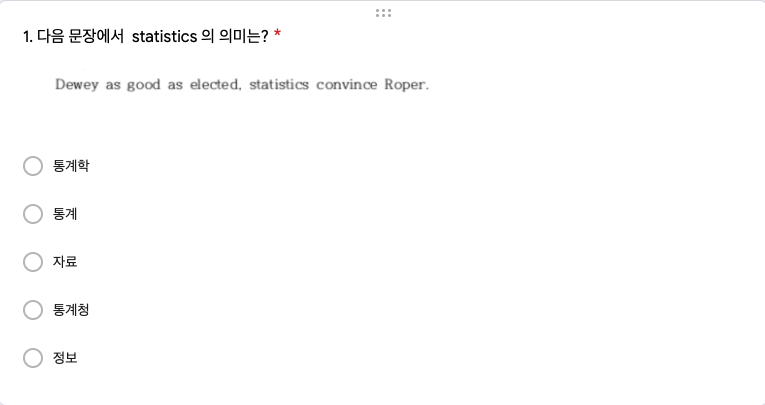
\includegraphics[width=1\linewidth]{./pics/Quiz210302_01} \end{flushleft}

\subsection{Roper(Counts)}\label{ropercounts}

\begin{longtable}[]{@{}
  >{\raggedright\arraybackslash}p{(\linewidth - 12\tabcolsep) * \real{0.1667}}
  >{\centering\arraybackslash}p{(\linewidth - 12\tabcolsep) * \real{0.1250}}
  >{\centering\arraybackslash}p{(\linewidth - 12\tabcolsep) * \real{0.0972}}
  >{\centering\arraybackslash}p{(\linewidth - 12\tabcolsep) * \real{0.0972}}
  >{\centering\arraybackslash}p{(\linewidth - 12\tabcolsep) * \real{0.1250}}
  >{\centering\arraybackslash}p{(\linewidth - 12\tabcolsep) * \real{0.0972}}
  >{\centering\arraybackslash}p{(\linewidth - 12\tabcolsep) * \real{0.0972}}@{}}
\toprule\noalign{}
\begin{minipage}[b]{\linewidth}\raggedright
~
\end{minipage} & \begin{minipage}[b]{\linewidth}\centering
통계학
\end{minipage} & \begin{minipage}[b]{\linewidth}\centering
통계
\end{minipage} & \begin{minipage}[b]{\linewidth}\centering
자료
\end{minipage} & \begin{minipage}[b]{\linewidth}\centering
통계청
\end{minipage} & \begin{minipage}[b]{\linewidth}\centering
정보
\end{minipage} & \begin{minipage}[b]{\linewidth}\centering
계
\end{minipage} \\
\midrule\noalign{}
\endhead
\bottomrule\noalign{}
\endlastfoot
\textbf{Red} & 26 & 230 & 25 & 6 & 5 & 292 \\
\textbf{Black} & 13 & 244 & 14 & 8 & 5 & 284 \\
\textbf{계} & 39 & 474 & 39 & 14 & 10 & 576 \\
\end{longtable}

\begin{longtable}[]{@{}
  >{\raggedleft\arraybackslash}p{(\linewidth - 4\tabcolsep) * \real{0.2361}}
  >{\raggedleft\arraybackslash}p{(\linewidth - 4\tabcolsep) * \real{0.0694}}
  >{\raggedleft\arraybackslash}p{(\linewidth - 4\tabcolsep) * \real{0.1389}}@{}}
\caption{Pearson's Chi-squared test: \texttt{.}}\tabularnewline
\toprule\noalign{}
\begin{minipage}[b]{\linewidth}\raggedleft
Test statistic
\end{minipage} & \begin{minipage}[b]{\linewidth}\raggedleft
df
\end{minipage} & \begin{minipage}[b]{\linewidth}\raggedleft
P value
\end{minipage} \\
\midrule\noalign{}
\endfirsthead
\toprule\noalign{}
\begin{minipage}[b]{\linewidth}\raggedleft
Test statistic
\end{minipage} & \begin{minipage}[b]{\linewidth}\raggedleft
df
\end{minipage} & \begin{minipage}[b]{\linewidth}\raggedleft
P value
\end{minipage} \\
\midrule\noalign{}
\endhead
\bottomrule\noalign{}
\endlastfoot
8.026 & 4 & 0.09065 \\
\end{longtable}

Q1의 집계 결과가 Red, Black 간에 통계적으로 유의한 차이가 있는지 알아보기 위하여 카이제곱 테스트를 수행하였습니다.

그 결과 카이제곱 통계량은 8.03, 자유도는 4, p-value 는 0.0906이므로 Red, Black 간에 통계적으로 유의한 차이를 보이지 않습니다.

실제로 닮은 게 느껴집니까?

\subsection{Roper(\%)}\label{roper}

\begin{longtable}[]{@{}
  >{\centering\arraybackslash}p{(\linewidth - 10\tabcolsep) * \real{0.1250}}
  >{\centering\arraybackslash}p{(\linewidth - 10\tabcolsep) * \real{0.0972}}
  >{\centering\arraybackslash}p{(\linewidth - 10\tabcolsep) * \real{0.0972}}
  >{\centering\arraybackslash}p{(\linewidth - 10\tabcolsep) * \real{0.1250}}
  >{\centering\arraybackslash}p{(\linewidth - 10\tabcolsep) * \real{0.0972}}
  >{\centering\arraybackslash}p{(\linewidth - 10\tabcolsep) * \real{0.1111}}@{}}
\toprule\noalign{}
\begin{minipage}[b]{\linewidth}\centering
통계학
\end{minipage} & \begin{minipage}[b]{\linewidth}\centering
통계
\end{minipage} & \begin{minipage}[b]{\linewidth}\centering
자료
\end{minipage} & \begin{minipage}[b]{\linewidth}\centering
통계청
\end{minipage} & \begin{minipage}[b]{\linewidth}\centering
정보
\end{minipage} & \begin{minipage}[b]{\linewidth}\centering
계
\end{minipage} \\
\midrule\noalign{}
\endhead
\bottomrule\noalign{}
\endlastfoot
6.8 & 82.3 & 6.8 & 2.4 & 1.7 & 100.0 \\
\end{longtable}

정답률은 Red, Black 을 합하여 계산하는데, 82.3(\%) 입니다.

\section{Q2. Statistics is the science of learning from data, \ldots{}}\label{q2.-statistics-is-the-science-of-learning-from-data}

이 문장의 출처는 미국통계협회 (ASA, American Statistical Association) 의 홈페이지 등입니다 (American Statistical Association n.d.) .

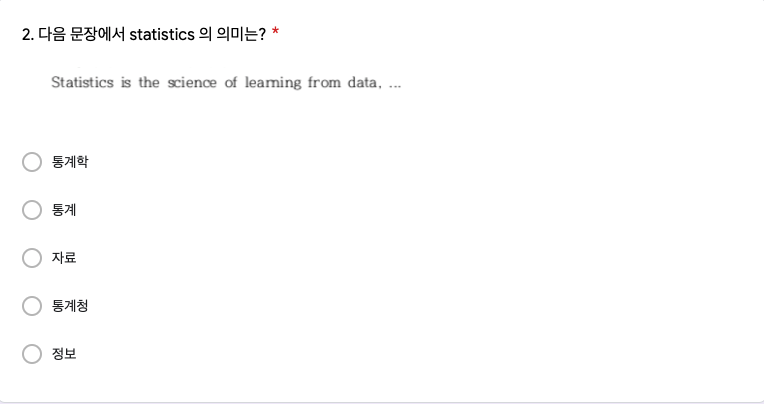
\includegraphics[width=1\linewidth]{./pics/Quiz210302_02}

\subsection{ASA(Counts)}\label{asacounts}

\begin{longtable}[]{@{}
  >{\raggedright\arraybackslash}p{(\linewidth - 12\tabcolsep) * \real{0.1667}}
  >{\centering\arraybackslash}p{(\linewidth - 12\tabcolsep) * \real{0.1250}}
  >{\centering\arraybackslash}p{(\linewidth - 12\tabcolsep) * \real{0.0972}}
  >{\centering\arraybackslash}p{(\linewidth - 12\tabcolsep) * \real{0.0972}}
  >{\centering\arraybackslash}p{(\linewidth - 12\tabcolsep) * \real{0.1250}}
  >{\centering\arraybackslash}p{(\linewidth - 12\tabcolsep) * \real{0.0972}}
  >{\centering\arraybackslash}p{(\linewidth - 12\tabcolsep) * \real{0.0972}}@{}}
\toprule\noalign{}
\begin{minipage}[b]{\linewidth}\raggedright
~
\end{minipage} & \begin{minipage}[b]{\linewidth}\centering
통계학
\end{minipage} & \begin{minipage}[b]{\linewidth}\centering
통계
\end{minipage} & \begin{minipage}[b]{\linewidth}\centering
자료
\end{minipage} & \begin{minipage}[b]{\linewidth}\centering
통계청
\end{minipage} & \begin{minipage}[b]{\linewidth}\centering
정보
\end{minipage} & \begin{minipage}[b]{\linewidth}\centering
계
\end{minipage} \\
\midrule\noalign{}
\endhead
\bottomrule\noalign{}
\endlastfoot
\textbf{Red} & 257 & 27 & 4 & 3 & 1 & 292 \\
\textbf{Black} & 262 & 14 & 3 & 2 & 3 & 284 \\
\textbf{계} & 519 & 41 & 7 & 5 & 4 & 576 \\
\end{longtable}

\begin{longtable}[]{@{}
  >{\raggedleft\arraybackslash}p{(\linewidth - 4\tabcolsep) * \real{0.2361}}
  >{\raggedleft\arraybackslash}p{(\linewidth - 4\tabcolsep) * \real{0.0694}}
  >{\raggedleft\arraybackslash}p{(\linewidth - 4\tabcolsep) * \real{0.1389}}@{}}
\caption{Pearson's Chi-squared test: \texttt{.}}\tabularnewline
\toprule\noalign{}
\begin{minipage}[b]{\linewidth}\raggedleft
Test statistic
\end{minipage} & \begin{minipage}[b]{\linewidth}\raggedleft
df
\end{minipage} & \begin{minipage}[b]{\linewidth}\raggedleft
P value
\end{minipage} \\
\midrule\noalign{}
\endfirsthead
\toprule\noalign{}
\begin{minipage}[b]{\linewidth}\raggedleft
Test statistic
\end{minipage} & \begin{minipage}[b]{\linewidth}\raggedleft
df
\end{minipage} & \begin{minipage}[b]{\linewidth}\raggedleft
P value
\end{minipage} \\
\midrule\noalign{}
\endhead
\bottomrule\noalign{}
\endlastfoot
5.403 & 4 & 0.2484 \\
\end{longtable}

Q2의 집계 결과가 Red, Black 간에 통계적으로 유의한 차이가 있는지 알아보기 위하여 카이제곱 테스트를 수행하였습니다.

그 결과 카이제곱 통계량은 5.403, 자유도는 4, p-value 는 0.2484이므로 Red, Black 간에 통계적으로 유의한 차이를 보이지 않습니다.

실제로 닮은 게 느껴집니까?

\subsection{ASA(\%)}\label{asa}

\begin{longtable}[]{@{}
  >{\centering\arraybackslash}p{(\linewidth - 10\tabcolsep) * \real{0.1250}}
  >{\centering\arraybackslash}p{(\linewidth - 10\tabcolsep) * \real{0.0972}}
  >{\centering\arraybackslash}p{(\linewidth - 10\tabcolsep) * \real{0.0972}}
  >{\centering\arraybackslash}p{(\linewidth - 10\tabcolsep) * \real{0.1250}}
  >{\centering\arraybackslash}p{(\linewidth - 10\tabcolsep) * \real{0.0972}}
  >{\centering\arraybackslash}p{(\linewidth - 10\tabcolsep) * \real{0.1250}}@{}}
\toprule\noalign{}
\begin{minipage}[b]{\linewidth}\centering
통계학
\end{minipage} & \begin{minipage}[b]{\linewidth}\centering
통계
\end{minipage} & \begin{minipage}[b]{\linewidth}\centering
자료
\end{minipage} & \begin{minipage}[b]{\linewidth}\centering
통계청
\end{minipage} & \begin{minipage}[b]{\linewidth}\centering
정보
\end{minipage} & \begin{minipage}[b]{\linewidth}\centering
계
\end{minipage} \\
\midrule\noalign{}
\endhead
\bottomrule\noalign{}
\endlastfoot
90.10 & 7.12 & 1.22 & 0.87 & 0.69 & 100.00 \\
\end{longtable}

정답률은 Red, Black 을 합하여 계산하는데, 90.1(\%) 입니다.

\section{Q3. How to lie with statistics}\label{q3.-how-to-lie-with-statistics}

이 문장은 Darrel Huff가 저술한 책 제목입니다 (Huff 1954) .

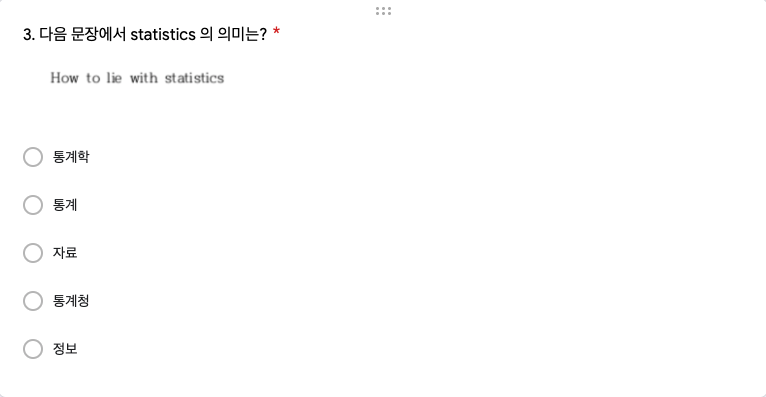
\includegraphics[width=1\linewidth]{./pics/Quiz210302_03}

\subsection{D.Huff(Counts)}\label{d.huffcounts}

\begin{longtable}[]{@{}
  >{\raggedright\arraybackslash}p{(\linewidth - 12\tabcolsep) * \real{0.1667}}
  >{\centering\arraybackslash}p{(\linewidth - 12\tabcolsep) * \real{0.1250}}
  >{\centering\arraybackslash}p{(\linewidth - 12\tabcolsep) * \real{0.0972}}
  >{\centering\arraybackslash}p{(\linewidth - 12\tabcolsep) * \real{0.0972}}
  >{\centering\arraybackslash}p{(\linewidth - 12\tabcolsep) * \real{0.1250}}
  >{\centering\arraybackslash}p{(\linewidth - 12\tabcolsep) * \real{0.0972}}
  >{\centering\arraybackslash}p{(\linewidth - 12\tabcolsep) * \real{0.0972}}@{}}
\toprule\noalign{}
\begin{minipage}[b]{\linewidth}\raggedright
~
\end{minipage} & \begin{minipage}[b]{\linewidth}\centering
통계학
\end{minipage} & \begin{minipage}[b]{\linewidth}\centering
통계
\end{minipage} & \begin{minipage}[b]{\linewidth}\centering
자료
\end{minipage} & \begin{minipage}[b]{\linewidth}\centering
통계청
\end{minipage} & \begin{minipage}[b]{\linewidth}\centering
정보
\end{minipage} & \begin{minipage}[b]{\linewidth}\centering
계
\end{minipage} \\
\midrule\noalign{}
\endhead
\bottomrule\noalign{}
\endlastfoot
\textbf{Red} & 14 & 204 & 41 & 14 & 19 & 292 \\
\textbf{Black} & 16 & 213 & 28 & 6 & 21 & 284 \\
\textbf{계} & 30 & 417 & 69 & 20 & 40 & 576 \\
\end{longtable}

\begin{longtable}[]{@{}
  >{\raggedleft\arraybackslash}p{(\linewidth - 4\tabcolsep) * \real{0.2361}}
  >{\raggedleft\arraybackslash}p{(\linewidth - 4\tabcolsep) * \real{0.0694}}
  >{\raggedleft\arraybackslash}p{(\linewidth - 4\tabcolsep) * \real{0.1389}}@{}}
\caption{Pearson's Chi-squared test: \texttt{.}}\tabularnewline
\toprule\noalign{}
\begin{minipage}[b]{\linewidth}\raggedleft
Test statistic
\end{minipage} & \begin{minipage}[b]{\linewidth}\raggedleft
df
\end{minipage} & \begin{minipage}[b]{\linewidth}\raggedleft
P value
\end{minipage} \\
\midrule\noalign{}
\endfirsthead
\toprule\noalign{}
\begin{minipage}[b]{\linewidth}\raggedleft
Test statistic
\end{minipage} & \begin{minipage}[b]{\linewidth}\raggedleft
df
\end{minipage} & \begin{minipage}[b]{\linewidth}\raggedleft
P value
\end{minipage} \\
\midrule\noalign{}
\endhead
\bottomrule\noalign{}
\endlastfoot
5.967 & 4 & 0.2016 \\
\end{longtable}

Q3의 집계 결과가 Red, Black 간에 통계적으로 유의한 차이가 있는지 알아보기 위하여 카이제곱 테스트를 수행하였습니다.

그 결과 카이제곱 통계량은 5.967, 자유도는 4, p-value 는 0.2016이므로 Red, Black 간에 통계적으로 유의한 차이를 보이지 않습니다.

실제로 닮은 게 느껴집니까?

\subsection{D.Huff(\%)}\label{d.huff}

\begin{longtable}[]{@{}
  >{\centering\arraybackslash}p{(\linewidth - 10\tabcolsep) * \real{0.1250}}
  >{\centering\arraybackslash}p{(\linewidth - 10\tabcolsep) * \real{0.0972}}
  >{\centering\arraybackslash}p{(\linewidth - 10\tabcolsep) * \real{0.0972}}
  >{\centering\arraybackslash}p{(\linewidth - 10\tabcolsep) * \real{0.1250}}
  >{\centering\arraybackslash}p{(\linewidth - 10\tabcolsep) * \real{0.0972}}
  >{\centering\arraybackslash}p{(\linewidth - 10\tabcolsep) * \real{0.1111}}@{}}
\toprule\noalign{}
\begin{minipage}[b]{\linewidth}\centering
통계학
\end{minipage} & \begin{minipage}[b]{\linewidth}\centering
통계
\end{minipage} & \begin{minipage}[b]{\linewidth}\centering
자료
\end{minipage} & \begin{minipage}[b]{\linewidth}\centering
통계청
\end{minipage} & \begin{minipage}[b]{\linewidth}\centering
정보
\end{minipage} & \begin{minipage}[b]{\linewidth}\centering
계
\end{minipage} \\
\midrule\noalign{}
\endhead
\bottomrule\noalign{}
\endlastfoot
5.2 & 72.4 & 12.0 & 3.5 & 6.9 & 100.0 \\
\end{longtable}

정답률은 Red, Black 을 합하여 계산하는데, 72.4(\%) 입니다.

\section{Q4. 종부세}\label{q4.-uxc885uxbd80uxc138}

질문지의 선택지에 부연 설명을 추가하여 응답을 왜곡할 수 있다는 우려는 설문조사 설계에서 잘 알려진 문제입니다. 이러한 현상은 `응답 편향(response bias)' 또는 '질문지 편향(questionnaire bias)'의 한 형태로 간주되며, 다양한 연구에서 이에 대한 사례와 분석이 이루어졌습니다.

``A Catalog of Biases in Questionnaires''
이 논문은 질문지에서 발생할 수 있는 48가지 편향 유형을 식별하고 분류하며, 각 유형에 대한 예시를 제공합니다. 특히, 질문의 형식과 응답 옵션의 설계가 응답자의 선택에 어떻게 영향을 미칠 수 있는지를 다루고 있습니다 (Boynton and Greenhalgh 2002).

``Response Biases in Standardised Surveys'' by Kathrin Bogner \& Uta Landrock
이 문서는 표준화된 설문조사에서 발생하는 응답 편향에 대해 설명하며, 질문의 형식과 응답 옵션이 응답자의 반응에 미치는 영향을 분석합니다 (Bogner and Landrock 2016).

``Biased Questions: How to Identify \& Fix Them in Surveys''
이 자료는 편향된 질문을 식별하고 수정하는 방법에 대해 설명하며, 부연 설명이 포함된 선택지가 응답자의 선택에 어떻게 영향을 줄 수 있는지를 다룹니다 (Genroe 2020).

NBS(전국지표조사)가 2024년 7월25일 발표한 종합부동산세 관련 여론조사 문항을 편집하여 선택지에 부연설명을 붙였을 때 응답에 어느 정도의 영향을 미치는 지 알아보고자 하였습니다 (중앙선거여론조사심의위원회 2024). 지난 학기에는 응답에 영향을 미친다는 것이 통계적으로 매우 유의한 수준으로 관찰되었습니다. 그러나, 이번 학기는 그렇지 않네요.

``바람직한 논의이다''라는 선택지에 부연설명을 붙이거나(Red), ``부적절한 논의이다''라는 선택지에 부연설명을 붙였을 때(Black), 부연설명의 여부에 따라 응답이 달라지는 지 살펴본 결과 기대와는 달리 통계적으로 유의한 수준의 차이를 관찰하지 못하였습니다.

앞에서 본 바와 같이 Red, Black 두 집단은 출석부의 다섯 변수에 대하여 랜덤화 과정을 거쳐서 가장 닮은 구성을 찾은 것이기에 Q1, Q2, Q3의 응답 결과도 매우 닮게 나오는데 만약 부연설명이 효과가 없다면 Q4에서의 응답도 닮게 나왔을 것입니다.

지난 학기들과 달리 통계적으로 유의한 차이를 관찰하지 못한 이유를 따져 볼 필요가 있겠습니다.

\subsection{질문지 선택지에 부연설명}\label{uxc9c8uxbb38uxc9c0-uxc120uxd0dduxc9c0uxc5d0-uxbd80uxc5f0uxc124uxba85}

\begin{flushleft}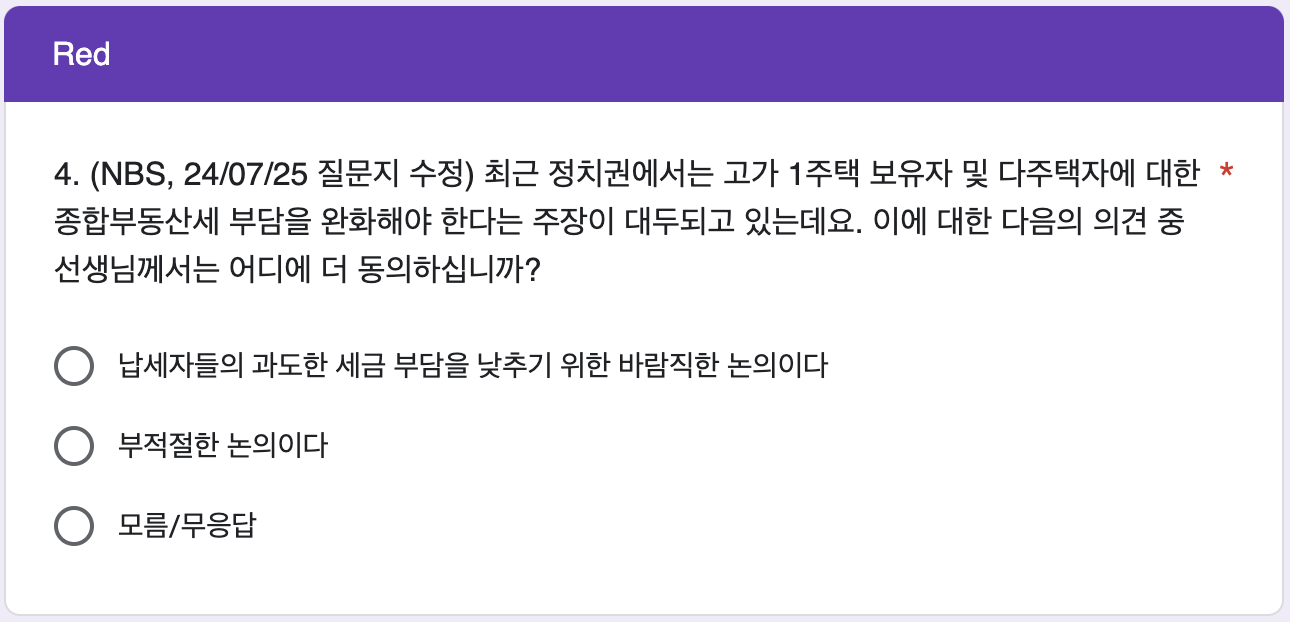
\includegraphics[width=0.67\linewidth]{./pics/Quiz240902_Q4_Red} \end{flushleft}

\begin{flushleft}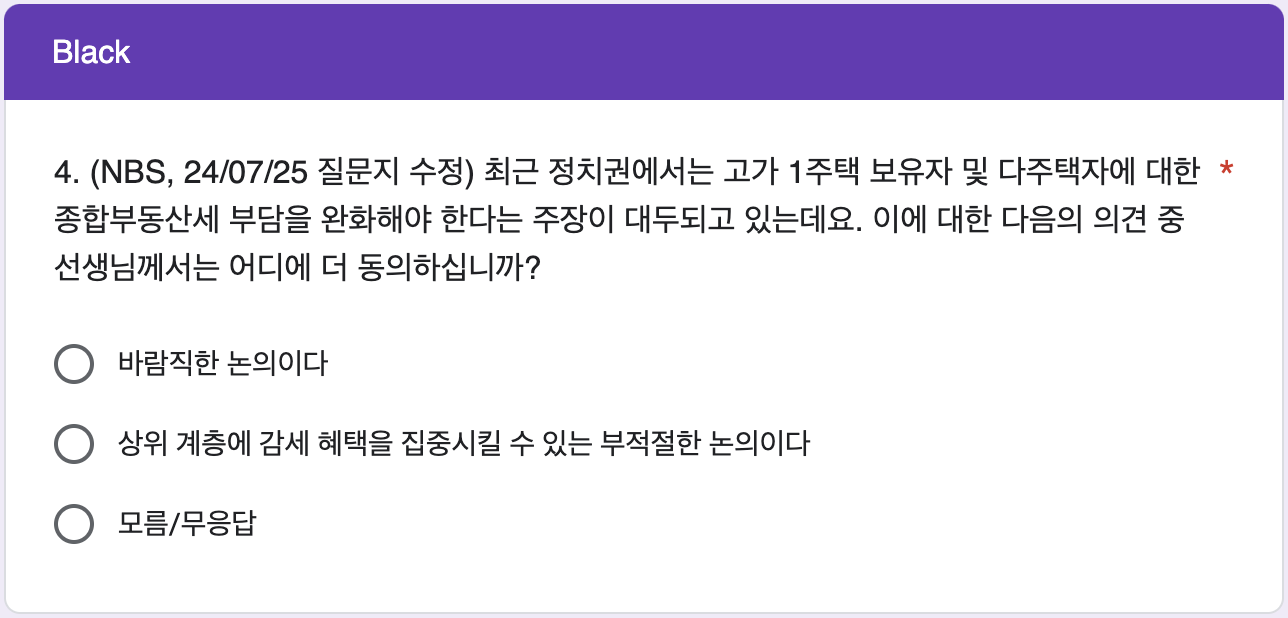
\includegraphics[width=0.67\linewidth]{./pics/Quiz240902_Q4_Black} \end{flushleft}

\subsection{집계}\label{uxc9d1uxacc4}

\begin{longtable}[]{@{}
  >{\raggedright\arraybackslash}p{(\linewidth - 8\tabcolsep) * \real{0.3023}}
  >{\centering\arraybackslash}p{(\linewidth - 8\tabcolsep) * \real{0.2326}}
  >{\centering\arraybackslash}p{(\linewidth - 8\tabcolsep) * \real{0.2326}}
  >{\centering\arraybackslash}p{(\linewidth - 8\tabcolsep) * \real{0.1628}}
  >{\centering\arraybackslash}p{(\linewidth - 8\tabcolsep) * \real{0.0698}}@{}}
\toprule\noalign{}
\begin{minipage}[b]{\linewidth}\raggedright
~
\end{minipage} & \begin{minipage}[b]{\linewidth}\centering
바람직한 논의이다
\end{minipage} & \begin{minipage}[b]{\linewidth}\centering
부적절한 논의이다
\end{minipage} & \begin{minipage}[b]{\linewidth}\centering
모름/무응답
\end{minipage} & \begin{minipage}[b]{\linewidth}\centering
계
\end{minipage} \\
\midrule\noalign{}
\endhead
\bottomrule\noalign{}
\endlastfoot
\textbf{Red(바람직한 논의에
부연설명)} & 95 & 113 & 84 & 292 \\
\textbf{Black(부적절한 논의에
부연설명)} & 72 & 130 & 82 & 284 \\
\textbf{계} & 167 & 243 & 166 & 576 \\
\end{longtable}

\begin{longtable}[]{@{}
  >{\raggedleft\arraybackslash}p{(\linewidth - 4\tabcolsep) * \real{0.2361}}
  >{\raggedleft\arraybackslash}p{(\linewidth - 4\tabcolsep) * \real{0.0694}}
  >{\raggedleft\arraybackslash}p{(\linewidth - 4\tabcolsep) * \real{0.1389}}@{}}
\caption{Pearson's Chi-squared test: \texttt{.}}\tabularnewline
\toprule\noalign{}
\begin{minipage}[b]{\linewidth}\raggedleft
Test statistic
\end{minipage} & \begin{minipage}[b]{\linewidth}\raggedleft
df
\end{minipage} & \begin{minipage}[b]{\linewidth}\raggedleft
P value
\end{minipage} \\
\midrule\noalign{}
\endfirsthead
\toprule\noalign{}
\begin{minipage}[b]{\linewidth}\raggedleft
Test statistic
\end{minipage} & \begin{minipage}[b]{\linewidth}\raggedleft
df
\end{minipage} & \begin{minipage}[b]{\linewidth}\raggedleft
P value
\end{minipage} \\
\midrule\noalign{}
\endhead
\bottomrule\noalign{}
\endlastfoot
4.271 & 2 & 0.1182 \\
\end{longtable}

Q4의 Red에는 종합부동산세 부담을 완화해야 한다는 주장에 대하여 바람직한 논의라는 쪽에 긍정적인 부연설명을 붙였는데, 292명이 응답한 가운데 95명이 ``바람직한 논의이다''라는 반응을 보이고, 113명이 ``부적절한 논의이다''라는 반응을 보입니다.

Black에는 같은 주장에 대하여 부적절한 논의라는 쪽에 부정적인 부연설명을 붙였는데, 284명이 응답한 가운데 72명이 ``바람직한 논의이다''라는 반응을 보이고, 130명이 ``부적절한 논의이다''라는 반응을 보입니다.

그리고 ``모름/무응답''에 답한 인원은 Red에 84명, Black 에 82명이 응답하였습니다.

지난 학기 자료들에서 볼 수 있다시피 카이제곱 테스트는 이와 같은 상황에서 부연설명의 유무가 응답에 미치는 영향이 대부분 통계적으로 유의하다는 것을 보여 줍니다.

그런데, 이번 학기는 매우 예외적으로 그렇지 않은 경우가 관찰되었습니다.

카이제곱 통계량은 4.271, 자유도는 2, p-value 는 0.1182으로 부연설명을 어떻게 붙이느냐에 따라 반응이 다르게 나온다는 것을 보여주고 싶었지만 실제로 관찰된 차이는 Q1 \textasciitilde{} Q3와 마찬가지로 통계적으로 유의한 수준은 아닙니다.

여기서 부연설명이 응답에 영향을 끼치지 않는다고 가정해 봅시다.

그렇다면 Red, Black 의 응답은 Q1\textasciitilde Q3 에서와 같이 랜덤화 효과에 의하여 통계적으로 유의한 차이를 보이지 않을 것입니다.

그런데 실제로 관찰된 카이제곱 통계값과 P-value 는 통계적으로 유의한 차이를 보여 주지 못하는 수준입니다.

따라서 부연설명이 영향을 끼치지 않는다는 가정을 받아들일 수밖에 없게 되었습니다.

지난 학기 자료들이 모두 통계적으로 유의한 차이를 보여 주었던 것과는 달리 이번 학기에 유독 통계적으로 유의한 차이를 보이지 않는 이유는 무엇일까요?

\subsection{\% 비교.}\label{uxbe44uxad50.}

\begin{longtable}[]{@{}
  >{\raggedright\arraybackslash}p{(\linewidth - 8\tabcolsep) * \real{0.2955}}
  >{\centering\arraybackslash}p{(\linewidth - 8\tabcolsep) * \real{0.2273}}
  >{\centering\arraybackslash}p{(\linewidth - 8\tabcolsep) * \real{0.2273}}
  >{\centering\arraybackslash}p{(\linewidth - 8\tabcolsep) * \real{0.1591}}
  >{\centering\arraybackslash}p{(\linewidth - 8\tabcolsep) * \real{0.0909}}@{}}
\toprule\noalign{}
\begin{minipage}[b]{\linewidth}\raggedright
~
\end{minipage} & \begin{minipage}[b]{\linewidth}\centering
바람직한 논의이다
\end{minipage} & \begin{minipage}[b]{\linewidth}\centering
부적절한 논의이다
\end{minipage} & \begin{minipage}[b]{\linewidth}\centering
모름/무응답
\end{minipage} & \begin{minipage}[b]{\linewidth}\centering
계
\end{minipage} \\
\midrule\noalign{}
\endhead
\bottomrule\noalign{}
\endlastfoot
\textbf{Red(바람직한 논의에
부연설명)} & 32.5 & 38.7 & 28.8 & 100.0 \\
\textbf{Black(부적절한 논의에
부연설명)} & 25.4 & 45.8 & 28.9 & 100.0 \\
\end{longtable}

``바람직한 논의이다''에 부연설명을 붙인 Red에서 ``바람직한 논의이다''라고 응답하는 사람들의 백분율, 32.5(\%)은 ``부적절한 논의이다''에 부연설명을 붙인 Black 에서 ``바람직한 논의이다''라고 응답하는 사람들의 백분율, 25.4(\%) 보다 높습니다.

반면 ``부적절한 논의이다''에 부연설명을 붙인 Black 에서 ``부적절한 논의이다''라고 응답하는 사람들의 백분율, 45.8(\%)은 Red 에서 ``부적절한 논의이다''라고 응답하는 사람들의 백분율, 38.7(\%) 보다 높습니다.

부연설명을 어디에 붙이느냐에 따라 반응이 치우치는 것을 알 수 있지만 p-value 가 보여주듯이 \textbf{그 차이가 통계적으로 유의한 수준은 아닌 것}입니다.

\subsection{Mosaic Plot}\label{mosaic-plot}

\begin{verbatim}
## Keep up to date with changes at https://tidyverse.org/blog/
\end{verbatim}

\pandocbounded{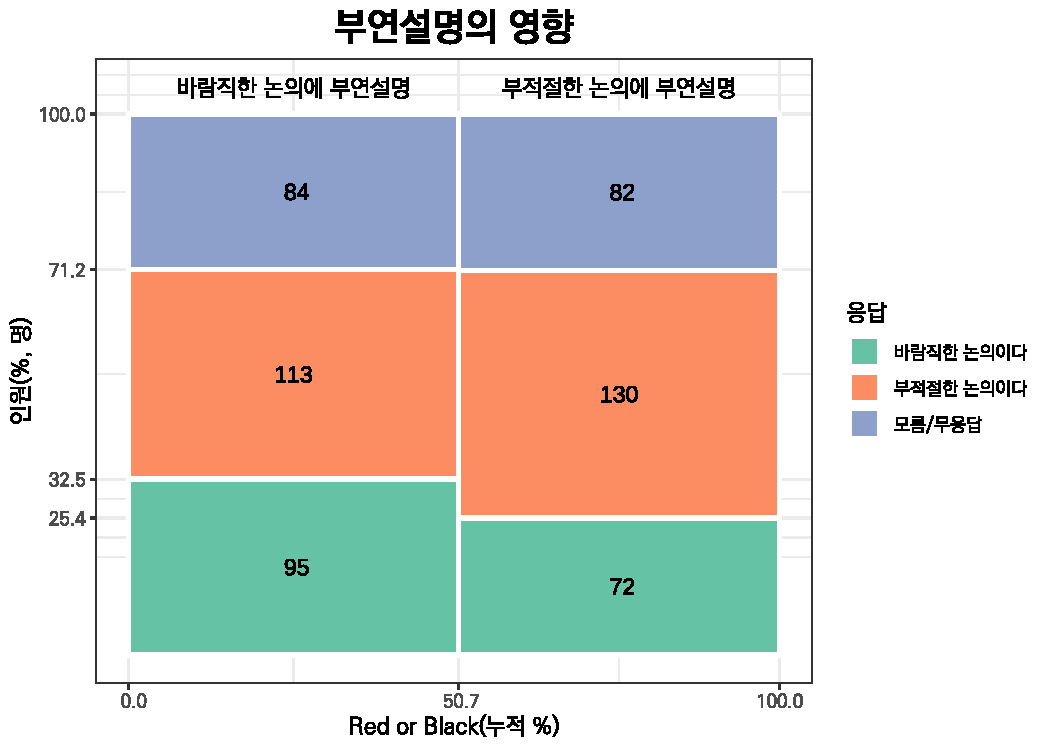
\includegraphics[keepaspectratio]{Quiz_report_2025_files/figure-latex/unnamed-chunk-14-1.pdf}}

Mosaic Plot 은 이 집계결과를 시각적으로 잘 보여줍니다.

``바람직한 논의이다''에 부연설명을 붙인 Red 에서 ``바람직힌 논의이다''라고 응답한 백분율이 ``부적절한 논의이다''에 부연설명을 붙인 Black 에서 ``바람직한 논의이다''라고 응답한 백분율보다 높고, Black 에서 ``부적절한 논의이다''라고 응답한 백분율은 Red 에서 ``부적절한 논의이다''라고 응답한 백분율보다 월등히 높습니다.

\section{마감 시간으로부터 제출 시간의 분포}\label{uxb9c8uxac10-uxc2dcuxac04uxc73cuxb85cuxbd80uxd130-uxc81cuxcd9c-uxc2dcuxac04uxc758-uxbd84uxd3ec}

\subsection{분포표}\label{uxbd84uxd3ecuxd45c}

\begin{longtable}[]{@{}
  >{\raggedright\arraybackslash}p{(\linewidth - 30\tabcolsep) * \real{0.1121}}
  >{\centering\arraybackslash}p{(\linewidth - 30\tabcolsep) * \real{0.0654}}
  >{\centering\arraybackslash}p{(\linewidth - 30\tabcolsep) * \real{0.0654}}
  >{\centering\arraybackslash}p{(\linewidth - 30\tabcolsep) * \real{0.0654}}
  >{\centering\arraybackslash}p{(\linewidth - 30\tabcolsep) * \real{0.0654}}
  >{\centering\arraybackslash}p{(\linewidth - 30\tabcolsep) * \real{0.0654}}
  >{\centering\arraybackslash}p{(\linewidth - 30\tabcolsep) * \real{0.0561}}
  >{\centering\arraybackslash}p{(\linewidth - 30\tabcolsep) * \real{0.0561}}
  >{\centering\arraybackslash}p{(\linewidth - 30\tabcolsep) * \real{0.0561}}
  >{\centering\arraybackslash}p{(\linewidth - 30\tabcolsep) * \real{0.0561}}
  >{\centering\arraybackslash}p{(\linewidth - 30\tabcolsep) * \real{0.0561}}
  >{\centering\arraybackslash}p{(\linewidth - 30\tabcolsep) * \real{0.0561}}
  >{\centering\arraybackslash}p{(\linewidth - 30\tabcolsep) * \real{0.0561}}
  >{\centering\arraybackslash}p{(\linewidth - 30\tabcolsep) * \real{0.0561}}
  >{\centering\arraybackslash}p{(\linewidth - 30\tabcolsep) * \real{0.0561}}
  >{\centering\arraybackslash}p{(\linewidth - 30\tabcolsep) * \real{0.0561}}@{}}
\caption{일 단위}\tabularnewline
\toprule\noalign{}
\begin{minipage}[b]{\linewidth}\raggedright
~
\end{minipage} & \begin{minipage}[b]{\linewidth}\centering
14일
\end{minipage} & \begin{minipage}[b]{\linewidth}\centering
13일
\end{minipage} & \begin{minipage}[b]{\linewidth}\centering
12일
\end{minipage} & \begin{minipage}[b]{\linewidth}\centering
11일
\end{minipage} & \begin{minipage}[b]{\linewidth}\centering
10일
\end{minipage} & \begin{minipage}[b]{\linewidth}\centering
9일
\end{minipage} & \begin{minipage}[b]{\linewidth}\centering
8일
\end{minipage} & \begin{minipage}[b]{\linewidth}\centering
7일
\end{minipage} & \begin{minipage}[b]{\linewidth}\centering
6일
\end{minipage} & \begin{minipage}[b]{\linewidth}\centering
5일
\end{minipage} & \begin{minipage}[b]{\linewidth}\centering
4일
\end{minipage} & \begin{minipage}[b]{\linewidth}\centering
3일
\end{minipage} & \begin{minipage}[b]{\linewidth}\centering
2일
\end{minipage} & \begin{minipage}[b]{\linewidth}\centering
1일
\end{minipage} & \begin{minipage}[b]{\linewidth}\centering
계
\end{minipage} \\
\midrule\noalign{}
\endfirsthead
\toprule\noalign{}
\begin{minipage}[b]{\linewidth}\raggedright
~
\end{minipage} & \begin{minipage}[b]{\linewidth}\centering
14일
\end{minipage} & \begin{minipage}[b]{\linewidth}\centering
13일
\end{minipage} & \begin{minipage}[b]{\linewidth}\centering
12일
\end{minipage} & \begin{minipage}[b]{\linewidth}\centering
11일
\end{minipage} & \begin{minipage}[b]{\linewidth}\centering
10일
\end{minipage} & \begin{minipage}[b]{\linewidth}\centering
9일
\end{minipage} & \begin{minipage}[b]{\linewidth}\centering
8일
\end{minipage} & \begin{minipage}[b]{\linewidth}\centering
7일
\end{minipage} & \begin{minipage}[b]{\linewidth}\centering
6일
\end{minipage} & \begin{minipage}[b]{\linewidth}\centering
5일
\end{minipage} & \begin{minipage}[b]{\linewidth}\centering
4일
\end{minipage} & \begin{minipage}[b]{\linewidth}\centering
3일
\end{minipage} & \begin{minipage}[b]{\linewidth}\centering
2일
\end{minipage} & \begin{minipage}[b]{\linewidth}\centering
1일
\end{minipage} & \begin{minipage}[b]{\linewidth}\centering
계
\end{minipage} \\
\midrule\noalign{}
\endhead
\bottomrule\noalign{}
\endlastfoot
\textbf{Red} & 46 & 11 & 6 & 11 & 6 & 14 & 10 & 42 & 21 & 19 & 15 & 30 & 35 & 26 & 292 \\
\textbf{Black} & 35 & 10 & 6 & 7 & 5 & 12 & 12 & 34 & 22 & 17 & 26 & 37 & 29 & 32 & 284 \\
\textbf{계} & 81 & 21 & 12 & 18 & 11 & 26 & 22 & 76 & 43 & 36 & 41 & 67 & 64 & 58 & 576 \\
\end{longtable}

분포표로부터 두 가지 문제를 살펴보겠습니다.

첫째, 날마다 고르게 제출하는가?

둘째, Red, Black 간에 통계적으로 유의한 차이가 있는가?

각 문제를 살펴보기 위해서는 분포표의 일부분을 대상으로 카이제곱 테스트를 수행합니다.

\subsection{날마다 고르게 제출하는가?}\label{uxb0a0uxb9c8uxb2e4-uxace0uxb974uxac8c-uxc81cuxcd9cuxd558uxb294uxac00}

\begin{longtable}[]{@{}
  >{\centering\arraybackslash}p{(\linewidth - 26\tabcolsep) * \real{0.0787}}
  >{\centering\arraybackslash}p{(\linewidth - 26\tabcolsep) * \real{0.0787}}
  >{\centering\arraybackslash}p{(\linewidth - 26\tabcolsep) * \real{0.0787}}
  >{\centering\arraybackslash}p{(\linewidth - 26\tabcolsep) * \real{0.0787}}
  >{\centering\arraybackslash}p{(\linewidth - 26\tabcolsep) * \real{0.0787}}
  >{\centering\arraybackslash}p{(\linewidth - 26\tabcolsep) * \real{0.0674}}
  >{\centering\arraybackslash}p{(\linewidth - 26\tabcolsep) * \real{0.0674}}
  >{\centering\arraybackslash}p{(\linewidth - 26\tabcolsep) * \real{0.0674}}
  >{\centering\arraybackslash}p{(\linewidth - 26\tabcolsep) * \real{0.0674}}
  >{\centering\arraybackslash}p{(\linewidth - 26\tabcolsep) * \real{0.0674}}
  >{\centering\arraybackslash}p{(\linewidth - 26\tabcolsep) * \real{0.0674}}
  >{\centering\arraybackslash}p{(\linewidth - 26\tabcolsep) * \real{0.0674}}
  >{\centering\arraybackslash}p{(\linewidth - 26\tabcolsep) * \real{0.0674}}
  >{\centering\arraybackslash}p{(\linewidth - 26\tabcolsep) * \real{0.0674}}@{}}
\toprule\noalign{}
\begin{minipage}[b]{\linewidth}\centering
14일
\end{minipage} & \begin{minipage}[b]{\linewidth}\centering
13일
\end{minipage} & \begin{minipage}[b]{\linewidth}\centering
12일
\end{minipage} & \begin{minipage}[b]{\linewidth}\centering
11일
\end{minipage} & \begin{minipage}[b]{\linewidth}\centering
10일
\end{minipage} & \begin{minipage}[b]{\linewidth}\centering
9일
\end{minipage} & \begin{minipage}[b]{\linewidth}\centering
8일
\end{minipage} & \begin{minipage}[b]{\linewidth}\centering
7일
\end{minipage} & \begin{minipage}[b]{\linewidth}\centering
6일
\end{minipage} & \begin{minipage}[b]{\linewidth}\centering
5일
\end{minipage} & \begin{minipage}[b]{\linewidth}\centering
4일
\end{minipage} & \begin{minipage}[b]{\linewidth}\centering
3일
\end{minipage} & \begin{minipage}[b]{\linewidth}\centering
2일
\end{minipage} & \begin{minipage}[b]{\linewidth}\centering
1일
\end{minipage} \\
\midrule\noalign{}
\endhead
\bottomrule\noalign{}
\endlastfoot
81 & 21 & 12 & 18 & 11 & 26 & 22 & 76 & 43 & 36 & 41 & 67 & 64 & 58 \\
\end{longtable}

\begin{longtable}[]{@{}
  >{\raggedleft\arraybackslash}p{(\linewidth - 4\tabcolsep) * \real{0.2361}}
  >{\raggedleft\arraybackslash}p{(\linewidth - 4\tabcolsep) * \real{0.0694}}
  >{\raggedleft\arraybackslash}p{(\linewidth - 4\tabcolsep) * \real{0.2500}}@{}}
\caption{Chi-squared test for given probabilities: \texttt{.}}\tabularnewline
\toprule\noalign{}
\begin{minipage}[b]{\linewidth}\raggedleft
Test statistic
\end{minipage} & \begin{minipage}[b]{\linewidth}\raggedleft
df
\end{minipage} & \begin{minipage}[b]{\linewidth}\raggedleft
P value
\end{minipage} \\
\midrule\noalign{}
\endfirsthead
\toprule\noalign{}
\begin{minipage}[b]{\linewidth}\raggedleft
Test statistic
\end{minipage} & \begin{minipage}[b]{\linewidth}\raggedleft
df
\end{minipage} & \begin{minipage}[b]{\linewidth}\raggedleft
P value
\end{minipage} \\
\midrule\noalign{}
\endhead
\bottomrule\noalign{}
\endlastfoot
184.8 & 13 & 1.766e-32 * * * \\
\end{longtable}

날마다 고르게 제출하는지 알아 보았습니다.

분포표의 ``계''행에서 '계'열을 제외하고 카이제곱테스트를 수행합니다.

분포표 만으로도 쉽게 파악할 수 있지만 카이제곱테스트가 명확히 해 줍니다.

카이제곱 통계량은 184.812, 자유도는 13, p-value 는 1.8e-32 이므로 결코 고르게 제출한다고 말할 수 없겠습니다.

막대그래프로 살펴 보겠습니다.

\subsection{막대그래프}\label{uxb9c9uxb300uxadf8uxb798uxd504}

\pandocbounded{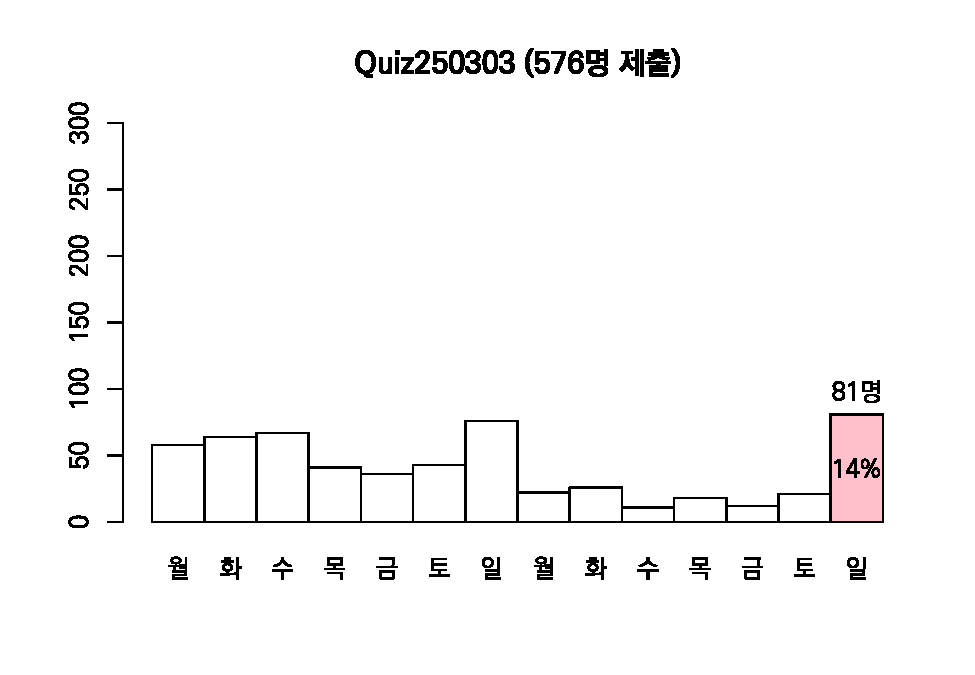
\includegraphics[keepaspectratio]{Quiz_report_2025_files/figure-latex/unnamed-chunk-18-1.pdf}}

막대그래프는 총 제출인원 576(명) 중에 81(명), 14(\%)가 마감일에 몰리는 것을 보여주고 있습니다.

\subsection{Red, Black 간에 닮았는가?}\label{red-black-uxac04uxc5d0-uxb2eeuxc558uxb294uxac00}

\begin{longtable}[]{@{}
  >{\raggedright\arraybackslash}p{(\linewidth - 28\tabcolsep) * \real{0.1188}}
  >{\centering\arraybackslash}p{(\linewidth - 28\tabcolsep) * \real{0.0693}}
  >{\centering\arraybackslash}p{(\linewidth - 28\tabcolsep) * \real{0.0693}}
  >{\centering\arraybackslash}p{(\linewidth - 28\tabcolsep) * \real{0.0693}}
  >{\centering\arraybackslash}p{(\linewidth - 28\tabcolsep) * \real{0.0693}}
  >{\centering\arraybackslash}p{(\linewidth - 28\tabcolsep) * \real{0.0693}}
  >{\centering\arraybackslash}p{(\linewidth - 28\tabcolsep) * \real{0.0594}}
  >{\centering\arraybackslash}p{(\linewidth - 28\tabcolsep) * \real{0.0594}}
  >{\centering\arraybackslash}p{(\linewidth - 28\tabcolsep) * \real{0.0594}}
  >{\centering\arraybackslash}p{(\linewidth - 28\tabcolsep) * \real{0.0594}}
  >{\centering\arraybackslash}p{(\linewidth - 28\tabcolsep) * \real{0.0594}}
  >{\centering\arraybackslash}p{(\linewidth - 28\tabcolsep) * \real{0.0594}}
  >{\centering\arraybackslash}p{(\linewidth - 28\tabcolsep) * \real{0.0594}}
  >{\centering\arraybackslash}p{(\linewidth - 28\tabcolsep) * \real{0.0594}}
  >{\centering\arraybackslash}p{(\linewidth - 28\tabcolsep) * \real{0.0594}}@{}}
\toprule\noalign{}
\begin{minipage}[b]{\linewidth}\raggedright
~
\end{minipage} & \begin{minipage}[b]{\linewidth}\centering
14일
\end{minipage} & \begin{minipage}[b]{\linewidth}\centering
13일
\end{minipage} & \begin{minipage}[b]{\linewidth}\centering
12일
\end{minipage} & \begin{minipage}[b]{\linewidth}\centering
11일
\end{minipage} & \begin{minipage}[b]{\linewidth}\centering
10일
\end{minipage} & \begin{minipage}[b]{\linewidth}\centering
9일
\end{minipage} & \begin{minipage}[b]{\linewidth}\centering
8일
\end{minipage} & \begin{minipage}[b]{\linewidth}\centering
7일
\end{minipage} & \begin{minipage}[b]{\linewidth}\centering
6일
\end{minipage} & \begin{minipage}[b]{\linewidth}\centering
5일
\end{minipage} & \begin{minipage}[b]{\linewidth}\centering
4일
\end{minipage} & \begin{minipage}[b]{\linewidth}\centering
3일
\end{minipage} & \begin{minipage}[b]{\linewidth}\centering
2일
\end{minipage} & \begin{minipage}[b]{\linewidth}\centering
1일
\end{minipage} \\
\midrule\noalign{}
\endhead
\bottomrule\noalign{}
\endlastfoot
\textbf{Red} & 46 & 11 & 6 & 11 & 6 & 14 & 10 & 42 & 21 & 19 & 15 & 30 & 35 & 26 \\
\textbf{Black} & 35 & 10 & 6 & 7 & 5 & 12 & 12 & 34 & 22 & 17 & 26 & 37 & 29 & 32 \\
\end{longtable}

\begin{longtable}[]{@{}
  >{\raggedleft\arraybackslash}p{(\linewidth - 4\tabcolsep) * \real{0.2361}}
  >{\raggedleft\arraybackslash}p{(\linewidth - 4\tabcolsep) * \real{0.0694}}
  >{\raggedleft\arraybackslash}p{(\linewidth - 4\tabcolsep) * \real{0.1389}}@{}}
\caption{Pearson's Chi-squared test: \texttt{.}}\tabularnewline
\toprule\noalign{}
\begin{minipage}[b]{\linewidth}\raggedleft
Test statistic
\end{minipage} & \begin{minipage}[b]{\linewidth}\raggedleft
df
\end{minipage} & \begin{minipage}[b]{\linewidth}\raggedleft
P value
\end{minipage} \\
\midrule\noalign{}
\endfirsthead
\toprule\noalign{}
\begin{minipage}[b]{\linewidth}\raggedleft
Test statistic
\end{minipage} & \begin{minipage}[b]{\linewidth}\raggedleft
df
\end{minipage} & \begin{minipage}[b]{\linewidth}\raggedleft
P value
\end{minipage} \\
\midrule\noalign{}
\endhead
\bottomrule\noalign{}
\endlastfoot
8.59 & 13 & 0.8032 \\
\end{longtable}

제출시간의 분포가 Red, Black 간에 닮았는지 알아 보았습니다.

이번에는 분포표의 첫번째와 두번째 행, '계'열을 제외한 나머지 열에 대해서 카이제곱테스트를 수행합니다.

카이제곱 통계량은 8.590, 자유도는 13, p-value 는 0.8032 이므로 제출 시간의 분포는 Red, Black 간에 통계적으로 유의한 차이가 관찰되지 않습니다.

이 사실을 Mosaic Plot 을 이용하여 시각적으로 살펴보겠습니다.

닮았다고 느껴지나요?

\subsection{Mosaic Plot}\label{mosaic-plot-1}

\pandocbounded{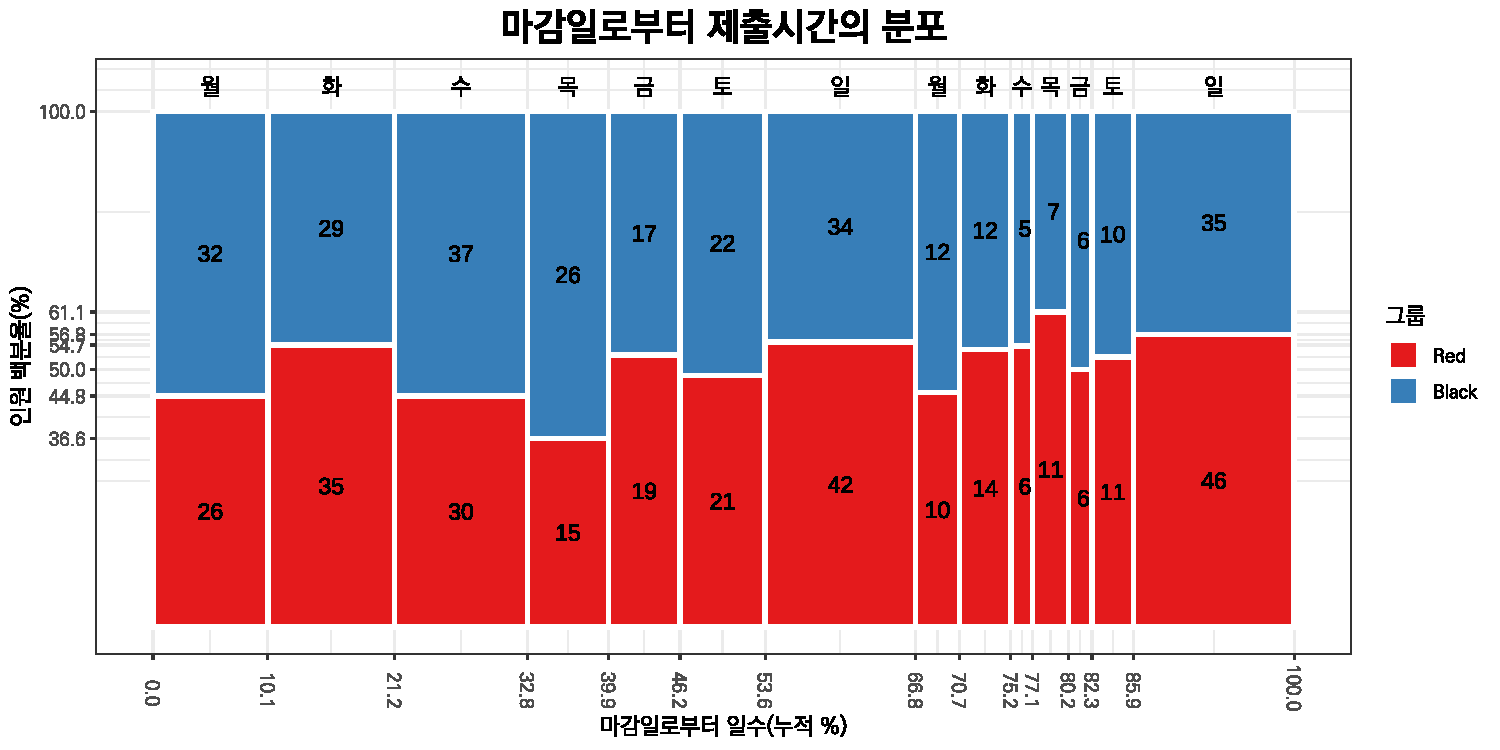
\includegraphics[keepaspectratio]{Quiz_report_2025_files/figure-latex/unnamed-chunk-20-1.pdf}}

\chapter{2주차 데이터 실험 집계}\label{uxc8fcuxcc28-uxb370uxc774uxd130-uxc2e4uxd5d8-uxc9d1uxacc4-1}

\section{실험의 목적}\label{uxc2e4uxd5d8uxc758-uxbaa9uxc801-1}

2주차 구글 예습 설문지 집계결과를 분석합니다.

Q1\textasciitilde Q6에서는 랜덤화의 효과로 Red, Black 이 얼마나 닮았는지 알아봅니다.

Q7에서는 같은 눈속임 그래프인데 원형그래프의 각도를 속일 떄(Red)와 막대그래프의 높이를 속일 때(Black) 오류를 지각하는 데 차이가 있는지 알아봅니다.

끝으로 제출시간의 분포가 날마다 고른지, Red, Black 간에는 닮았는지 알아봅니다.

\subsection{Red, Black을 잘못 표시한 사람들}\label{red-blackuxc744-uxc798uxbabb-uxd45cuxc2dcuxd55c-uxc0acuxb78cuxb4e4-1}

\begin{longtable}[]{@{}
  >{\centering\arraybackslash}p{(\linewidth - 6\tabcolsep) * \real{0.3056}}
  >{\centering\arraybackslash}p{(\linewidth - 6\tabcolsep) * \real{0.1528}}
  >{\centering\arraybackslash}p{(\linewidth - 6\tabcolsep) * \real{0.2083}}
  >{\centering\arraybackslash}p{(\linewidth - 6\tabcolsep) * \real{0.2083}}@{}}
\toprule\noalign{}
\begin{minipage}[b]{\linewidth}\centering
제출시간
\end{minipage} & \begin{minipage}[b]{\linewidth}\centering
학번
\end{minipage} & \begin{minipage}[b]{\linewidth}\centering
랜덤화출석부
\end{minipage} & \begin{minipage}[b]{\linewidth}\centering
구글예습퀴즈
\end{minipage} \\
\midrule\noalign{}
\endhead
\bottomrule\noalign{}
\endlastfoot
2025-03-11 21:44:18 & 20223501 & Red & Black \\
2025-03-12 01:12:52 & 20246792 & Black & Red \\
2025-03-12 02:27:14 & 20242601 & Red & Black \\
2025-03-13 02:06:41 & 20246737 & Red & Black \\
2025-03-13 19:03:57 & 20241216 & Red & Black \\
2025-03-14 09:32:05 & 20241022 & Black & Red \\
2025-03-14 10:22:29 & 20231725 & Red & Black \\
2025-03-14 15:07:21 & 20243233 & Black & Red \\
2025-03-15 15:21:53 & 20213033 & Red & Black \\
2025-03-15 22:20:27 & 20241201 & Red & Black \\
2025-03-15 22:46:42 & 20243720 & Red & Black \\
2025-03-16 15:31:37 & 20223329 & Black & Red \\
2025-03-16 17:32:57 & 20211021 & Black & Red \\
2025-03-16 19:50:32 & 20241011 & Red & Black \\
2025-03-16 20:56:30 & 20213040 & Red & Black \\
2025-03-16 23:10:55 & 20241028 & Black & Red \\
2025-03-17 21:59:54 & 20242960 & Black & Red \\
2025-03-20 11:14:21 & 20246272 & Black & Red \\
2025-03-20 14:54:36 & 20246923 & Black & Red \\
2025-03-20 20:52:14 & 20242949 & Black & Red \\
2025-03-22 00:55:57 & 20246606 & Black & Red \\
2025-03-23 11:51:35 & 20242585 & Red & Black \\
2025-03-23 14:27:48 & 20243513 & Black & Red \\
2025-03-23 19:53:42 & 20227107 & Red & Black \\
\end{longtable}

\begin{longtable}[]{@{}
  >{\raggedright\arraybackslash}p{(\linewidth - 4\tabcolsep) * \real{0.3611}}
  >{\centering\arraybackslash}p{(\linewidth - 4\tabcolsep) * \real{0.2778}}
  >{\centering\arraybackslash}p{(\linewidth - 4\tabcolsep) * \real{0.3056}}@{}}
\toprule\noalign{}
\begin{minipage}[b]{\linewidth}\raggedright
~
\end{minipage} & \begin{minipage}[b]{\linewidth}\centering
Red(구글예습퀴즈)
\end{minipage} & \begin{minipage}[b]{\linewidth}\centering
Black(구글예습퀴즈)
\end{minipage} \\
\midrule\noalign{}
\endhead
\bottomrule\noalign{}
\endlastfoot
\textbf{Red(랜덤화출석부)} & 268 & 12 \\
\textbf{Black(랜덤화출석부)} & 12 & 269 \\
\textbf{계} & 280 & 281 \\
\end{longtable}

랜덤화출석부에 있는 Red, Black 과 실제 구글설문에 올린 Red, Black 이 다른 사람들의 수효는 24명입니다.

Red를 Black 이라고 한 사람이 12명, Black 을 Red 라고 한 사람이 12명입니다.

두 가지 방법으로 분석합니다.

우선 Red, Black 을 잘못 선택한 24명을 랜덤하게 둘로 나누면 어느 한 쪽 집단에 들어갈 기대인원은 24명을 둘로 나눈 12(명)이고, 표준오차는 24의 제곱근에 1/2을 곱해 준 2.4명이 됩니다.

실제로 Red를 Black 이라고 한 사람수, 12명이나 Black 을 Red 라고 한 사람수, 12명은 기대인원으로부터 표준오차 범위 안에 아주 잘 들어갑니다.

두 번째 분석 방법은 확률을 계산해 보는 것입니다.

Red, Black 을 잘못 선택한 24명을 랜덤하게 둘로 나눌 때, 실제로 관찰된 12명 이상이나 12명이하로 잘못 선택한 사람수가 나올 가능성은 얼마나 되는가 입니다.

이 경우 공평한 동전던지기를 확률 법칙으로 표현한 이항분포로부터 계산할 수 있습니다.

시행횟수가 24이고 한 번 시행에서 성공확률이 1/2 인 이항분포에서 성공횟수가 12이하이거나 12이상을 관찰할 확률은 1.161입니다.

공평한 동전 던지기에서 앞면이 12개 이하 나오는 확률은 12개 이상 나오는 확률과 같기 때문에 사실상 한쪽만 계산해서 2배 해 주면 됩니다.

이 값을 p-value 라고 하는데, p-value가 0.05보다 작을 때 \textbf{통계적으로 유의한 차이를 관찰}하였다고 말합니다.

즉, 공평한 동전을 던지는 것과 같은 과정이라고 가정하였을 때 실제로 관찰된 값들이 가정으로부터 얼마나 떨어져 있는지를 표현한 것입니다.

0.05, 즉 1/20은 이런 실험을 스무 번 정도 반복하면 1번 나올 정도로 드문 사건을 의미합니다.

즉 가정이 타당하다면 나오기 힘든 결과라는 것입니다.

그런데 Red, Black 을 잘못 표시한 사람들의 분포에서 관찰된 p-value 는 0.05와는 비교도 안될 정도로 큰 값입니다.

따라서 두 집단이 랜덤화 효과가 작동하여 \textbf{통계적으로 유의한 차이를 보이지 않는다}고 할 수 있습니다.

\subsection{응답인원의 Red, Black}\label{uxc751uxb2f5uxc778uxc6d0uxc758-red-black-1}

Red 로 응답한 인원은 280명, Black 에 응답한 인원은 281명입니다.

전체 응답인원 561 명을 랜덤하게 둘로 나눌 때 어느 한 쪽의 기대인원은 전체 응답인원의 절반인 280.5명이고, 표준오차는 전체 응답인원의 제곱근에 1/2을 곱해 준 11.8 명입니다.

따라서 Red, Black 각 그룹에 관찰된 인원은 기대인원으로부터 표준오차 범위, 혹은 두배의 표준오차 범위 안에 들어갑니다.

\section{Q1. 춘추전국시대에 국가통계관리의 중요성 강조}\label{q1.-uxcd98uxcd94uxc804uxad6duxc2dcuxb300uxc5d0-uxad6duxac00uxd1b5uxacc4uxad00uxb9acuxc758-uxc911uxc694uxc131-uxac15uxc870}

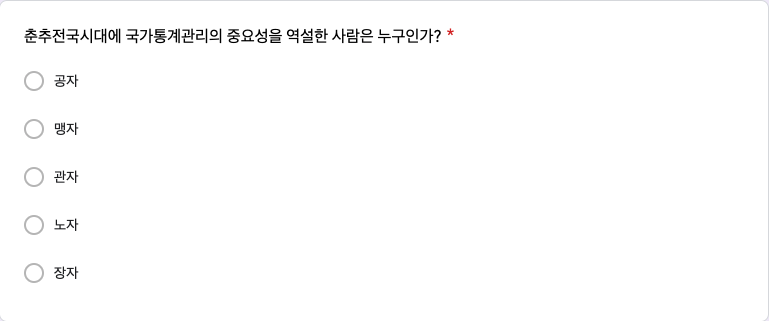
\includegraphics[width=0.75\linewidth]{./pics/Quiz210309_01}

\subsection{관자(집계표)}\label{uxad00uxc790uxc9d1uxacc4uxd45c}

\begin{longtable}[]{@{}
  >{\raggedright\arraybackslash}p{(\linewidth - 12\tabcolsep) * \real{0.1667}}
  >{\centering\arraybackslash}p{(\linewidth - 12\tabcolsep) * \real{0.0972}}
  >{\centering\arraybackslash}p{(\linewidth - 12\tabcolsep) * \real{0.0972}}
  >{\centering\arraybackslash}p{(\linewidth - 12\tabcolsep) * \real{0.0972}}
  >{\centering\arraybackslash}p{(\linewidth - 12\tabcolsep) * \real{0.0972}}
  >{\centering\arraybackslash}p{(\linewidth - 12\tabcolsep) * \real{0.0972}}
  >{\centering\arraybackslash}p{(\linewidth - 12\tabcolsep) * \real{0.0972}}@{}}
\toprule\noalign{}
\begin{minipage}[b]{\linewidth}\raggedright
~
\end{minipage} & \begin{minipage}[b]{\linewidth}\centering
공자
\end{minipage} & \begin{minipage}[b]{\linewidth}\centering
맹자
\end{minipage} & \begin{minipage}[b]{\linewidth}\centering
관자
\end{minipage} & \begin{minipage}[b]{\linewidth}\centering
노자
\end{minipage} & \begin{minipage}[b]{\linewidth}\centering
장자
\end{minipage} & \begin{minipage}[b]{\linewidth}\centering
계
\end{minipage} \\
\midrule\noalign{}
\endhead
\bottomrule\noalign{}
\endlastfoot
\textbf{Red} & 40 & 9 & 224 & 8 & 1 & 282 \\
\textbf{Black} & 25 & 17 & 223 & 11 & 5 & 281 \\
\textbf{계} & 65 & 26 & 447 & 19 & 6 & 563 \\
\end{longtable}

\begin{longtable}[]{@{}
  >{\raggedleft\arraybackslash}p{(\linewidth - 4\tabcolsep) * \real{0.2361}}
  >{\raggedleft\arraybackslash}p{(\linewidth - 4\tabcolsep) * \real{0.0694}}
  >{\raggedleft\arraybackslash}p{(\linewidth - 4\tabcolsep) * \real{0.1389}}@{}}
\caption{Pearson's Chi-squared test with simulated p-value
(based on 2000 replicates): \texttt{.}}\tabularnewline
\toprule\noalign{}
\begin{minipage}[b]{\linewidth}\raggedleft
Test statistic
\end{minipage} & \begin{minipage}[b]{\linewidth}\raggedleft
df
\end{minipage} & \begin{minipage}[b]{\linewidth}\raggedleft
P value
\end{minipage} \\
\midrule\noalign{}
\endfirsthead
\toprule\noalign{}
\begin{minipage}[b]{\linewidth}\raggedleft
Test statistic
\end{minipage} & \begin{minipage}[b]{\linewidth}\raggedleft
df
\end{minipage} & \begin{minipage}[b]{\linewidth}\raggedleft
P value
\end{minipage} \\
\midrule\noalign{}
\endhead
\bottomrule\noalign{}
\endlastfoot
9.064 & NA & 0.06247 \\
\end{longtable}

Q1의 집계 결과가 Red, Black 간에 통계적으로 유의한 차이가 있는지 알아보기 위하여 카이제곱 테스트를 수행하였습니다.

그 결과 카이제곱 통계량은 9.06, 자유도는 NA , p-value 는 0.0625이므로 Red, Black 간에 통계적으로 유의한 차이를 보이지 않습니다.

실제로 닮은 게 느껴집니까?

\subsection{관자(\%)}\label{uxad00uxc790}

\begin{longtable}[]{@{}
  >{\centering\arraybackslash}p{(\linewidth - 10\tabcolsep) * \real{0.0972}}
  >{\centering\arraybackslash}p{(\linewidth - 10\tabcolsep) * \real{0.0972}}
  >{\centering\arraybackslash}p{(\linewidth - 10\tabcolsep) * \real{0.0972}}
  >{\centering\arraybackslash}p{(\linewidth - 10\tabcolsep) * \real{0.0972}}
  >{\centering\arraybackslash}p{(\linewidth - 10\tabcolsep) * \real{0.0972}}
  >{\centering\arraybackslash}p{(\linewidth - 10\tabcolsep) * \real{0.1111}}@{}}
\toprule\noalign{}
\begin{minipage}[b]{\linewidth}\centering
공자
\end{minipage} & \begin{minipage}[b]{\linewidth}\centering
맹자
\end{minipage} & \begin{minipage}[b]{\linewidth}\centering
관자
\end{minipage} & \begin{minipage}[b]{\linewidth}\centering
노자
\end{minipage} & \begin{minipage}[b]{\linewidth}\centering
장자
\end{minipage} & \begin{minipage}[b]{\linewidth}\centering
계
\end{minipage} \\
\midrule\noalign{}
\endhead
\bottomrule\noalign{}
\endlastfoot
11.5 & 4.6 & 79.4 & 3.4 & 1.1 & 100.0 \\
\end{longtable}

정답률은 Red, Black 을 합하여 계산하는데, 79.4(\%) 입니다.

\section{Q2. 국가정책을 수립하는 데 통계의 역할}\label{q2.-uxad6duxac00uxc815uxcc45uxc744-uxc218uxb9bduxd558uxb294-uxb370-uxd1b5uxacc4uxc758-uxc5eduxd560}


\includegraphics[width=0.75\linewidth]{./pics/Quiz210309_02}

\subsection{통계의 중요성(집계표)}\label{uxd1b5uxacc4uxc758-uxc911uxc694uxc131uxc9d1uxacc4uxd45c}

\begin{longtable}[]{@{}
  >{\raggedright\arraybackslash}p{(\linewidth - 12\tabcolsep) * \real{0.1062}}
  >{\centering\arraybackslash}p{(\linewidth - 12\tabcolsep) * \real{0.2035}}
  >{\centering\arraybackslash}p{(\linewidth - 12\tabcolsep) * \real{0.1858}}
  >{\centering\arraybackslash}p{(\linewidth - 12\tabcolsep) * \real{0.0973}}
  >{\centering\arraybackslash}p{(\linewidth - 12\tabcolsep) * \real{0.1593}}
  >{\centering\arraybackslash}p{(\linewidth - 12\tabcolsep) * \real{0.1947}}
  >{\centering\arraybackslash}p{(\linewidth - 12\tabcolsep) * \real{0.0531}}@{}}
\toprule\noalign{}
\begin{minipage}[b]{\linewidth}\raggedright
~
\end{minipage} & \begin{minipage}[b]{\linewidth}\centering
절대로 중요하지 않다
\end{minipage} & \begin{minipage}[b]{\linewidth}\centering
거의 중요하지 않다
\end{minipage} & \begin{minipage}[b]{\linewidth}\centering
보통이다
\end{minipage} & \begin{minipage}[b]{\linewidth}\centering
상당히 중요하다
\end{minipage} & \begin{minipage}[b]{\linewidth}\centering
절대적으로 중요하다
\end{minipage} & \begin{minipage}[b]{\linewidth}\centering
계
\end{minipage} \\
\midrule\noalign{}
\endhead
\bottomrule\noalign{}
\endlastfoot
\textbf{Red} & 0 & 2 & 9 & 94 & 177 & 282 \\
\textbf{Black} & 2 & 4 & 9 & 94 & 172 & 281 \\
\textbf{계} & 2 & 6 & 18 & 188 & 349 & 563 \\
\end{longtable}

\begin{longtable}[]{@{}
  >{\raggedleft\arraybackslash}p{(\linewidth - 4\tabcolsep) * \real{0.2361}}
  >{\raggedleft\arraybackslash}p{(\linewidth - 4\tabcolsep) * \real{0.0694}}
  >{\raggedleft\arraybackslash}p{(\linewidth - 4\tabcolsep) * \real{0.1389}}@{}}
\caption{Pearson's Chi-squared test with simulated p-value
(based on 2000 replicates): \texttt{.}}\tabularnewline
\toprule\noalign{}
\begin{minipage}[b]{\linewidth}\raggedleft
Test statistic
\end{minipage} & \begin{minipage}[b]{\linewidth}\raggedleft
df
\end{minipage} & \begin{minipage}[b]{\linewidth}\raggedleft
P value
\end{minipage} \\
\midrule\noalign{}
\endfirsthead
\toprule\noalign{}
\begin{minipage}[b]{\linewidth}\raggedleft
Test statistic
\end{minipage} & \begin{minipage}[b]{\linewidth}\raggedleft
df
\end{minipage} & \begin{minipage}[b]{\linewidth}\raggedleft
P value
\end{minipage} \\
\midrule\noalign{}
\endhead
\bottomrule\noalign{}
\endlastfoot
2.056 & NA & 0.6617 \\
\end{longtable}

Q2의 집계 결과가 Red, Black 간에 통계적으로 유의한 차이가 있는지 알아보기 위하여 카이제곱 테스트를 수행하였습니다.

그 결과 카이제곱 통계량은 2.056, 자유도는 NA, p-value 는 0.6617이므로 Red, Black 간에 통계적으로 유의한 차이를 보이지 않습니다.

실제로 닮은 게 느껴집니까?

\subsection{통계의 중요성(\%)}\label{uxd1b5uxacc4uxc758-uxc911uxc694uxc131}

\begin{longtable}[]{@{}
  >{\centering\arraybackslash}p{(\linewidth - 10\tabcolsep) * \real{0.2212}}
  >{\centering\arraybackslash}p{(\linewidth - 10\tabcolsep) * \real{0.2019}}
  >{\centering\arraybackslash}p{(\linewidth - 10\tabcolsep) * \real{0.1058}}
  >{\centering\arraybackslash}p{(\linewidth - 10\tabcolsep) * \real{0.1731}}
  >{\centering\arraybackslash}p{(\linewidth - 10\tabcolsep) * \real{0.2115}}
  >{\centering\arraybackslash}p{(\linewidth - 10\tabcolsep) * \real{0.0865}}@{}}
\toprule\noalign{}
\begin{minipage}[b]{\linewidth}\centering
절대로 중요하지 않다
\end{minipage} & \begin{minipage}[b]{\linewidth}\centering
거의 중요하지 않다
\end{minipage} & \begin{minipage}[b]{\linewidth}\centering
보통이다
\end{minipage} & \begin{minipage}[b]{\linewidth}\centering
상당히 중요하다
\end{minipage} & \begin{minipage}[b]{\linewidth}\centering
절대적으로 중요하다
\end{minipage} & \begin{minipage}[b]{\linewidth}\centering
계
\end{minipage} \\
\midrule\noalign{}
\endhead
\bottomrule\noalign{}
\endlastfoot
0.36 & 1.07 & 3.20 & 33.39 & 61.99 & 100.00 \\
\end{longtable}

정답률은 Red, Black 을 합하여 계산하는데, 62.0(\%) 입니다.

\section{Q3. 우리나라 생산가능인구 감소 시기}\label{q3.-uxc6b0uxb9acuxb098uxb77c-uxc0dduxc0b0uxac00uxb2a5uxc778uxad6c-uxac10uxc18c-uxc2dcuxae30}


\includegraphics[width=0.75\linewidth]{./pics/Quiz210309_03}

\subsection{생산가능인구 감소 시기(집계표)}\label{uxc0dduxc0b0uxac00uxb2a5uxc778uxad6c-uxac10uxc18c-uxc2dcuxae30uxc9d1uxacc4uxd45c}

\begin{longtable}[]{@{}
  >{\raggedright\arraybackslash}p{(\linewidth - 10\tabcolsep) * \real{0.1667}}
  >{\raggedleft\arraybackslash}p{(\linewidth - 10\tabcolsep) * \real{0.0972}}
  >{\raggedleft\arraybackslash}p{(\linewidth - 10\tabcolsep) * \real{0.0972}}
  >{\raggedleft\arraybackslash}p{(\linewidth - 10\tabcolsep) * \real{0.0972}}
  >{\raggedleft\arraybackslash}p{(\linewidth - 10\tabcolsep) * \real{0.0972}}
  >{\centering\arraybackslash}p{(\linewidth - 10\tabcolsep) * \real{0.0972}}@{}}
\toprule\noalign{}
\begin{minipage}[b]{\linewidth}\raggedright
~
\end{minipage} & \begin{minipage}[b]{\linewidth}\raggedleft
2012
\end{minipage} & \begin{minipage}[b]{\linewidth}\raggedleft
2017
\end{minipage} & \begin{minipage}[b]{\linewidth}\raggedleft
2022
\end{minipage} & \begin{minipage}[b]{\linewidth}\raggedleft
2027
\end{minipage} & \begin{minipage}[b]{\linewidth}\centering
계
\end{minipage} \\
\midrule\noalign{}
\endhead
\bottomrule\noalign{}
\endlastfoot
\textbf{Red} & 31 & 224 & 23 & 4 & 282 \\
\textbf{Black} & 23 & 227 & 25 & 6 & 281 \\
\textbf{계} & 54 & 451 & 48 & 10 & 563 \\
\end{longtable}

\begin{longtable}[]{@{}
  >{\raggedleft\arraybackslash}p{(\linewidth - 4\tabcolsep) * \real{0.2361}}
  >{\raggedleft\arraybackslash}p{(\linewidth - 4\tabcolsep) * \real{0.0694}}
  >{\raggedleft\arraybackslash}p{(\linewidth - 4\tabcolsep) * \real{0.1389}}@{}}
\caption{Pearson's Chi-squared test: \texttt{.}}\tabularnewline
\toprule\noalign{}
\begin{minipage}[b]{\linewidth}\raggedleft
Test statistic
\end{minipage} & \begin{minipage}[b]{\linewidth}\raggedleft
df
\end{minipage} & \begin{minipage}[b]{\linewidth}\raggedleft
P value
\end{minipage} \\
\midrule\noalign{}
\endfirsthead
\toprule\noalign{}
\begin{minipage}[b]{\linewidth}\raggedleft
Test statistic
\end{minipage} & \begin{minipage}[b]{\linewidth}\raggedleft
df
\end{minipage} & \begin{minipage}[b]{\linewidth}\raggedleft
P value
\end{minipage} \\
\midrule\noalign{}
\endhead
\bottomrule\noalign{}
\endlastfoot
1.687 & 3 & 0.6399 \\
\end{longtable}

Q3의 집계 결과가 Red, Black 간에 통계적으로 유의한 차이가 있는지 알아보기 위하여 카이제곱 테스트를 수행하였습니다.

그 결과 카이제곱 통계량은 1.687, 자유도는 3, p-value 는 0.6399이므로 Red, Black 간에 통계적으로 유의한 차이를 보이지 않습니다.

실제로 닮은 게 느껴집니까?

\subsection{생산가능인구 감소 시기(\%)}\label{uxc0dduxc0b0uxac00uxb2a5uxc778uxad6c-uxac10uxc18c-uxc2dcuxae30}

\begin{longtable}[]{@{}
  >{\raggedleft\arraybackslash}p{(\linewidth - 8\tabcolsep) * \real{0.0972}}
  >{\raggedleft\arraybackslash}p{(\linewidth - 8\tabcolsep) * \real{0.0972}}
  >{\raggedleft\arraybackslash}p{(\linewidth - 8\tabcolsep) * \real{0.0972}}
  >{\raggedleft\arraybackslash}p{(\linewidth - 8\tabcolsep) * \real{0.0972}}
  >{\centering\arraybackslash}p{(\linewidth - 8\tabcolsep) * \real{0.1111}}@{}}
\toprule\noalign{}
\begin{minipage}[b]{\linewidth}\raggedleft
2012
\end{minipage} & \begin{minipage}[b]{\linewidth}\raggedleft
2017
\end{minipage} & \begin{minipage}[b]{\linewidth}\raggedleft
2022
\end{minipage} & \begin{minipage}[b]{\linewidth}\raggedleft
2027
\end{minipage} & \begin{minipage}[b]{\linewidth}\centering
계
\end{minipage} \\
\midrule\noalign{}
\endhead
\bottomrule\noalign{}
\endlastfoot
9.6 & 80.1 & 8.5 & 1.8 & 100.0 \\
\end{longtable}

정답률은 Red, Black 을 합하여 계산하는데, 80.1(\%) 입니다.

\section{Q4. 우리나라 총인구 최대 시기}\label{q4.-uxc6b0uxb9acuxb098uxb77c-uxcd1duxc778uxad6c-uxcd5cuxb300-uxc2dcuxae30}


\includegraphics[width=0.75\linewidth]{./pics/Quiz230308_Q4}

\subsection{총인구 최대 시기(집계표)}\label{uxcd1duxc778uxad6c-uxcd5cuxb300-uxc2dcuxae30uxc9d1uxacc4uxd45c}

\begin{longtable}[]{@{}
  >{\raggedright\arraybackslash}p{(\linewidth - 10\tabcolsep) * \real{0.1667}}
  >{\raggedleft\arraybackslash}p{(\linewidth - 10\tabcolsep) * \real{0.0972}}
  >{\raggedleft\arraybackslash}p{(\linewidth - 10\tabcolsep) * \real{0.0972}}
  >{\raggedleft\arraybackslash}p{(\linewidth - 10\tabcolsep) * \real{0.0972}}
  >{\raggedleft\arraybackslash}p{(\linewidth - 10\tabcolsep) * \real{0.0972}}
  >{\centering\arraybackslash}p{(\linewidth - 10\tabcolsep) * \real{0.0972}}@{}}
\toprule\noalign{}
\begin{minipage}[b]{\linewidth}\raggedright
~
\end{minipage} & \begin{minipage}[b]{\linewidth}\raggedleft
2018
\end{minipage} & \begin{minipage}[b]{\linewidth}\raggedleft
2019
\end{minipage} & \begin{minipage}[b]{\linewidth}\raggedleft
2020
\end{minipage} & \begin{minipage}[b]{\linewidth}\raggedleft
2021
\end{minipage} & \begin{minipage}[b]{\linewidth}\centering
계
\end{minipage} \\
\midrule\noalign{}
\endhead
\bottomrule\noalign{}
\endlastfoot
\textbf{Red} & 47 & 27 & 205 & 3 & 282 \\
\textbf{Black} & 29 & 27 & 215 & 10 & 281 \\
\textbf{계} & 76 & 54 & 420 & 13 & 563 \\
\end{longtable}

\begin{longtable}[]{@{}
  >{\raggedleft\arraybackslash}p{(\linewidth - 4\tabcolsep) * \real{0.2361}}
  >{\raggedleft\arraybackslash}p{(\linewidth - 4\tabcolsep) * \real{0.0694}}
  >{\raggedleft\arraybackslash}p{(\linewidth - 4\tabcolsep) * \real{0.1667}}@{}}
\caption{Pearson's Chi-squared test with simulated p-value
(based on 2000 replicates): \texttt{.}}\tabularnewline
\toprule\noalign{}
\begin{minipage}[b]{\linewidth}\raggedleft
Test statistic
\end{minipage} & \begin{minipage}[b]{\linewidth}\raggedleft
df
\end{minipage} & \begin{minipage}[b]{\linewidth}\raggedleft
P value
\end{minipage} \\
\midrule\noalign{}
\endfirsthead
\toprule\noalign{}
\begin{minipage}[b]{\linewidth}\raggedleft
Test statistic
\end{minipage} & \begin{minipage}[b]{\linewidth}\raggedleft
df
\end{minipage} & \begin{minipage}[b]{\linewidth}\raggedleft
P value
\end{minipage} \\
\midrule\noalign{}
\endhead
\bottomrule\noalign{}
\endlastfoot
8.269 & NA & 0.03648 * \\
\end{longtable}

Q4의 집계 결과가 Red, Black 간에 통계적으로 유의한 차이가 있는지 알아보기 위하여 카이제곱 테스트를 수행하였습니다.

그 결과 카이제곱 통계량은 8.269, 자유도는 NA, p-value 는 0.0365이므로 Red, Black 간에 통계적으로 유의한 차이를 보이고 있습니다.

\subsection{총인구 최대 시기(\%)}\label{uxcd1duxc778uxad6c-uxcd5cuxb300-uxc2dcuxae30}

\begin{longtable}[]{@{}
  >{\raggedleft\arraybackslash}p{(\linewidth - 8\tabcolsep) * \real{0.0972}}
  >{\raggedleft\arraybackslash}p{(\linewidth - 8\tabcolsep) * \real{0.0972}}
  >{\raggedleft\arraybackslash}p{(\linewidth - 8\tabcolsep) * \real{0.0972}}
  >{\raggedleft\arraybackslash}p{(\linewidth - 8\tabcolsep) * \real{0.0972}}
  >{\centering\arraybackslash}p{(\linewidth - 8\tabcolsep) * \real{0.1111}}@{}}
\toprule\noalign{}
\begin{minipage}[b]{\linewidth}\raggedleft
2018
\end{minipage} & \begin{minipage}[b]{\linewidth}\raggedleft
2019
\end{minipage} & \begin{minipage}[b]{\linewidth}\raggedleft
2020
\end{minipage} & \begin{minipage}[b]{\linewidth}\raggedleft
2021
\end{minipage} & \begin{minipage}[b]{\linewidth}\centering
계
\end{minipage} \\
\midrule\noalign{}
\endhead
\bottomrule\noalign{}
\endlastfoot
13.5 & 9.6 & 74.6 & 2.3 & 100.0 \\
\end{longtable}

정답률은 Red, Black 을 합하여 계산하는데, 74.6(\%) 입니다.

\section{Q5. 소멸위험 단계 개선 지역}\label{q5.-uxc18cuxba78uxc704uxd5d8-uxb2e8uxacc4-uxac1cuxc120-uxc9c0uxc5ed}


\includegraphics[width=0.75\linewidth]{./pics/Quiz230308_Q5}

\subsection{소멸위험 단계 개선 지역(집계표)}\label{uxc18cuxba78uxc704uxd5d8-uxb2e8uxacc4-uxac1cuxc120-uxc9c0uxc5eduxc9d1uxacc4uxd45c}

\begin{longtable}[]{@{}
  >{\raggedright\arraybackslash}p{(\linewidth - 10\tabcolsep) * \real{0.1667}}
  >{\centering\arraybackslash}p{(\linewidth - 10\tabcolsep) * \real{0.0972}}
  >{\centering\arraybackslash}p{(\linewidth - 10\tabcolsep) * \real{0.0972}}
  >{\centering\arraybackslash}p{(\linewidth - 10\tabcolsep) * \real{0.0972}}
  >{\centering\arraybackslash}p{(\linewidth - 10\tabcolsep) * \real{0.0972}}
  >{\centering\arraybackslash}p{(\linewidth - 10\tabcolsep) * \real{0.0972}}@{}}
\toprule\noalign{}
\begin{minipage}[b]{\linewidth}\raggedright
~
\end{minipage} & \begin{minipage}[b]{\linewidth}\centering
서울
\end{minipage} & \begin{minipage}[b]{\linewidth}\centering
경기
\end{minipage} & \begin{minipage}[b]{\linewidth}\centering
세종
\end{minipage} & \begin{minipage}[b]{\linewidth}\centering
제주
\end{minipage} & \begin{minipage}[b]{\linewidth}\centering
계
\end{minipage} \\
\midrule\noalign{}
\endhead
\bottomrule\noalign{}
\endlastfoot
\textbf{Red} & 13 & 14 & 241 & 14 & 282 \\
\textbf{Black} & 9 & 14 & 245 & 13 & 281 \\
\textbf{계} & 22 & 28 & 486 & 27 & 563 \\
\end{longtable}

\begin{longtable}[]{@{}
  >{\raggedleft\arraybackslash}p{(\linewidth - 4\tabcolsep) * \real{0.2361}}
  >{\raggedleft\arraybackslash}p{(\linewidth - 4\tabcolsep) * \real{0.0694}}
  >{\raggedleft\arraybackslash}p{(\linewidth - 4\tabcolsep) * \real{0.1389}}@{}}
\caption{Pearson's Chi-squared test with simulated p-value
(based on 2000 replicates): \texttt{.}}\tabularnewline
\toprule\noalign{}
\begin{minipage}[b]{\linewidth}\raggedleft
Test statistic
\end{minipage} & \begin{minipage}[b]{\linewidth}\raggedleft
df
\end{minipage} & \begin{minipage}[b]{\linewidth}\raggedleft
P value
\end{minipage} \\
\midrule\noalign{}
\endfirsthead
\toprule\noalign{}
\begin{minipage}[b]{\linewidth}\raggedleft
Test statistic
\end{minipage} & \begin{minipage}[b]{\linewidth}\raggedleft
df
\end{minipage} & \begin{minipage}[b]{\linewidth}\raggedleft
P value
\end{minipage} \\
\midrule\noalign{}
\endhead
\bottomrule\noalign{}
\endlastfoot
0.7955 & NA & 0.8506 \\
\end{longtable}

Q5의 집계 결과가 Red, Black 간에 통계적으로 유의한 차이가 있는지 알아보기 위하여 카이제곱 테스트를 수행하였습니다.

그 결과 카이제곱 통계량은 0.795, 자유도는 NA, p-value 는 0.8506이므로 Red, Black 간에 통계적으로 유의한 차이를 보이지 않습니다.

실제로 닮은 게 느껴집니까?

\subsection{소멸위험 단계 개선 지역(\%)}\label{uxc18cuxba78uxc704uxd5d8-uxb2e8uxacc4-uxac1cuxc120-uxc9c0uxc5ed}

\begin{longtable}[]{@{}
  >{\centering\arraybackslash}p{(\linewidth - 8\tabcolsep) * \real{0.0972}}
  >{\centering\arraybackslash}p{(\linewidth - 8\tabcolsep) * \real{0.0972}}
  >{\centering\arraybackslash}p{(\linewidth - 8\tabcolsep) * \real{0.0972}}
  >{\centering\arraybackslash}p{(\linewidth - 8\tabcolsep) * \real{0.0972}}
  >{\centering\arraybackslash}p{(\linewidth - 8\tabcolsep) * \real{0.1111}}@{}}
\toprule\noalign{}
\begin{minipage}[b]{\linewidth}\centering
서울
\end{minipage} & \begin{minipage}[b]{\linewidth}\centering
경기
\end{minipage} & \begin{minipage}[b]{\linewidth}\centering
세종
\end{minipage} & \begin{minipage}[b]{\linewidth}\centering
제주
\end{minipage} & \begin{minipage}[b]{\linewidth}\centering
계
\end{minipage} \\
\midrule\noalign{}
\endhead
\bottomrule\noalign{}
\endlastfoot
3.9 & 5.0 & 86.3 & 4.8 & 100.0 \\
\end{longtable}

정답률은 Red, Black 을 합하여 계산하는데, 86.3(\%) 입니다.

\section{Q6. 조출생률과 합계출산율}\label{q6.-uxc870uxcd9cuxc0dduxb960uxacfc-uxd569uxacc4uxcd9cuxc0b0uxc728}

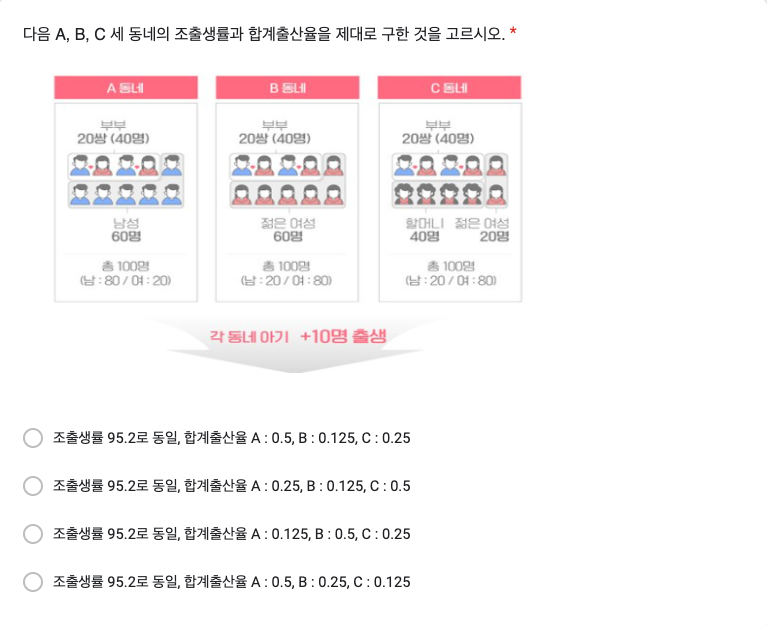
\includegraphics[width=0.75\linewidth]{./pics/Quiz230308_Q6}

\subsection{조출생률과 합계출산율(집계표)}\label{uxc870uxcd9cuxc0dduxb960uxacfc-uxd569uxacc4uxcd9cuxc0b0uxc728uxc9d1uxacc4uxd45c}

\begin{longtable}[]{@{}
  >{\raggedright\arraybackslash}p{(\linewidth - 10\tabcolsep) * \real{0.0839}}
  >{\centering\arraybackslash}p{(\linewidth - 10\tabcolsep) * \real{0.2308}}
  >{\centering\arraybackslash}p{(\linewidth - 10\tabcolsep) * \real{0.1888}}
  >{\centering\arraybackslash}p{(\linewidth - 10\tabcolsep) * \real{0.2308}}
  >{\centering\arraybackslash}p{(\linewidth - 10\tabcolsep) * \real{0.2238}}
  >{\centering\arraybackslash}p{(\linewidth - 10\tabcolsep) * \real{0.0420}}@{}}
\toprule\noalign{}
\begin{minipage}[b]{\linewidth}\raggedright
~
\end{minipage} & \begin{minipage}[b]{\linewidth}\centering
합계출산율 A : 0.5, B : 0.125,
C : 0.25
\end{minipage} & \begin{minipage}[b]{\linewidth}\centering
합계출산율 A : 0.25, B :
0.125, C : 0.5
\end{minipage} & \begin{minipage}[b]{\linewidth}\centering
합계출산율 A : 0.125, B : 0.5,
C : 0.25
\end{minipage} & \begin{minipage}[b]{\linewidth}\centering
합계출산율 A : 0.5, B : 0.25,
C : 0.125
\end{minipage} & \begin{minipage}[b]{\linewidth}\centering
계
\end{minipage} \\
\midrule\noalign{}
\endhead
\bottomrule\noalign{}
\endlastfoot
\textbf{Red} & 163 & 34 & 56 & 29 & 282 \\
\textbf{Black} & 140 & 56 & 48 & 37 & 281 \\
\textbf{계} & 303 & 90 & 104 & 66 & 563 \\
\end{longtable}

\begin{longtable}[]{@{}
  >{\raggedleft\arraybackslash}p{(\linewidth - 4\tabcolsep) * \real{0.2361}}
  >{\raggedleft\arraybackslash}p{(\linewidth - 4\tabcolsep) * \real{0.0694}}
  >{\raggedleft\arraybackslash}p{(\linewidth - 4\tabcolsep) * \real{0.1667}}@{}}
\caption{Pearson's Chi-squared test: \texttt{.}}\tabularnewline
\toprule\noalign{}
\begin{minipage}[b]{\linewidth}\raggedleft
Test statistic
\end{minipage} & \begin{minipage}[b]{\linewidth}\raggedleft
df
\end{minipage} & \begin{minipage}[b]{\linewidth}\raggedleft
P value
\end{minipage} \\
\midrule\noalign{}
\endfirsthead
\toprule\noalign{}
\begin{minipage}[b]{\linewidth}\raggedleft
Test statistic
\end{minipage} & \begin{minipage}[b]{\linewidth}\raggedleft
df
\end{minipage} & \begin{minipage}[b]{\linewidth}\raggedleft
P value
\end{minipage} \\
\midrule\noalign{}
\endhead
\bottomrule\noalign{}
\endlastfoot
8.707 & 3 & 0.03345 * \\
\end{longtable}

Q6의 집계 결과가 Red, Black 간에 통계적으로 유의한 차이가 있는지 알아보기 위하여 카이제곱 테스트를 수행하였습니다.

그 결과 카이제곱 통계량은 8.707, 자유도는 3, p-value 는 0.0335이므로 Red, Black 간에 통계적으로 유의한 차이를 보이고 있습니다.

\subsection{조출생률과 합계출산율(\%)}\label{uxc870uxcd9cuxc0dduxb960uxacfc-uxd569uxacc4uxcd9cuxc0b0uxc728}

\begin{longtable}[]{@{}
  >{\centering\arraybackslash}p{(\linewidth - 8\tabcolsep) * \real{0.2481}}
  >{\centering\arraybackslash}p{(\linewidth - 8\tabcolsep) * \real{0.2030}}
  >{\centering\arraybackslash}p{(\linewidth - 8\tabcolsep) * \real{0.2481}}
  >{\centering\arraybackslash}p{(\linewidth - 8\tabcolsep) * \real{0.2406}}
  >{\centering\arraybackslash}p{(\linewidth - 8\tabcolsep) * \real{0.0602}}@{}}
\toprule\noalign{}
\begin{minipage}[b]{\linewidth}\centering
합계출산율 A : 0.5, B : 0.125,
C : 0.25
\end{minipage} & \begin{minipage}[b]{\linewidth}\centering
합계출산율 A : 0.25, B :
0.125, C : 0.5
\end{minipage} & \begin{minipage}[b]{\linewidth}\centering
합계출산율 A : 0.125, B : 0.5,
C : 0.25
\end{minipage} & \begin{minipage}[b]{\linewidth}\centering
합계출산율 A : 0.5, B : 0.25,
C : 0.125
\end{minipage} & \begin{minipage}[b]{\linewidth}\centering
계
\end{minipage} \\
\midrule\noalign{}
\endhead
\bottomrule\noalign{}
\endlastfoot
53.8 & 16.0 & 18.5 & 11.7 & 100.0 \\
\end{longtable}

정답률은 Red, Black 을 합하여 계산하는데, 53.8(\%) 입니다.

\section{Q7. 눈속임 그래프(Cheating Charts)}\label{q7.-uxb208uxc18duxc784-uxadf8uxb798uxd504cheating-charts}

지난 학기까지 앞에 나오는 선지를 고르기 쉽다는 1번효과에 대한 질문을 만들어서 테스트해 왔지만 효과를 검증하기 어려워 문제를 바꿔 보았습니다.

언론방송에서 가끔 원형그래프나 막대그래프를 제시하면서 숫자와 그림이 맞지 않는 경우를 볼 수 있습니다.

여러분들은 그런 경우에 어떻게 인식하는 지 언론기관에서 발표한 눈속임 그래프를 보여줍니다.

Red에는 원형그래프의 각도를 속이고, Black 에는 막대그래프의 높이를 속여 어떤 응답이 나오는 지 살펴보았습니다.

여러분들은 대부분 눈속임 그래프에 속지 않고 있습니다.

언론기관들이 왜 이런 짓들을 하는지 궁금해집니다.

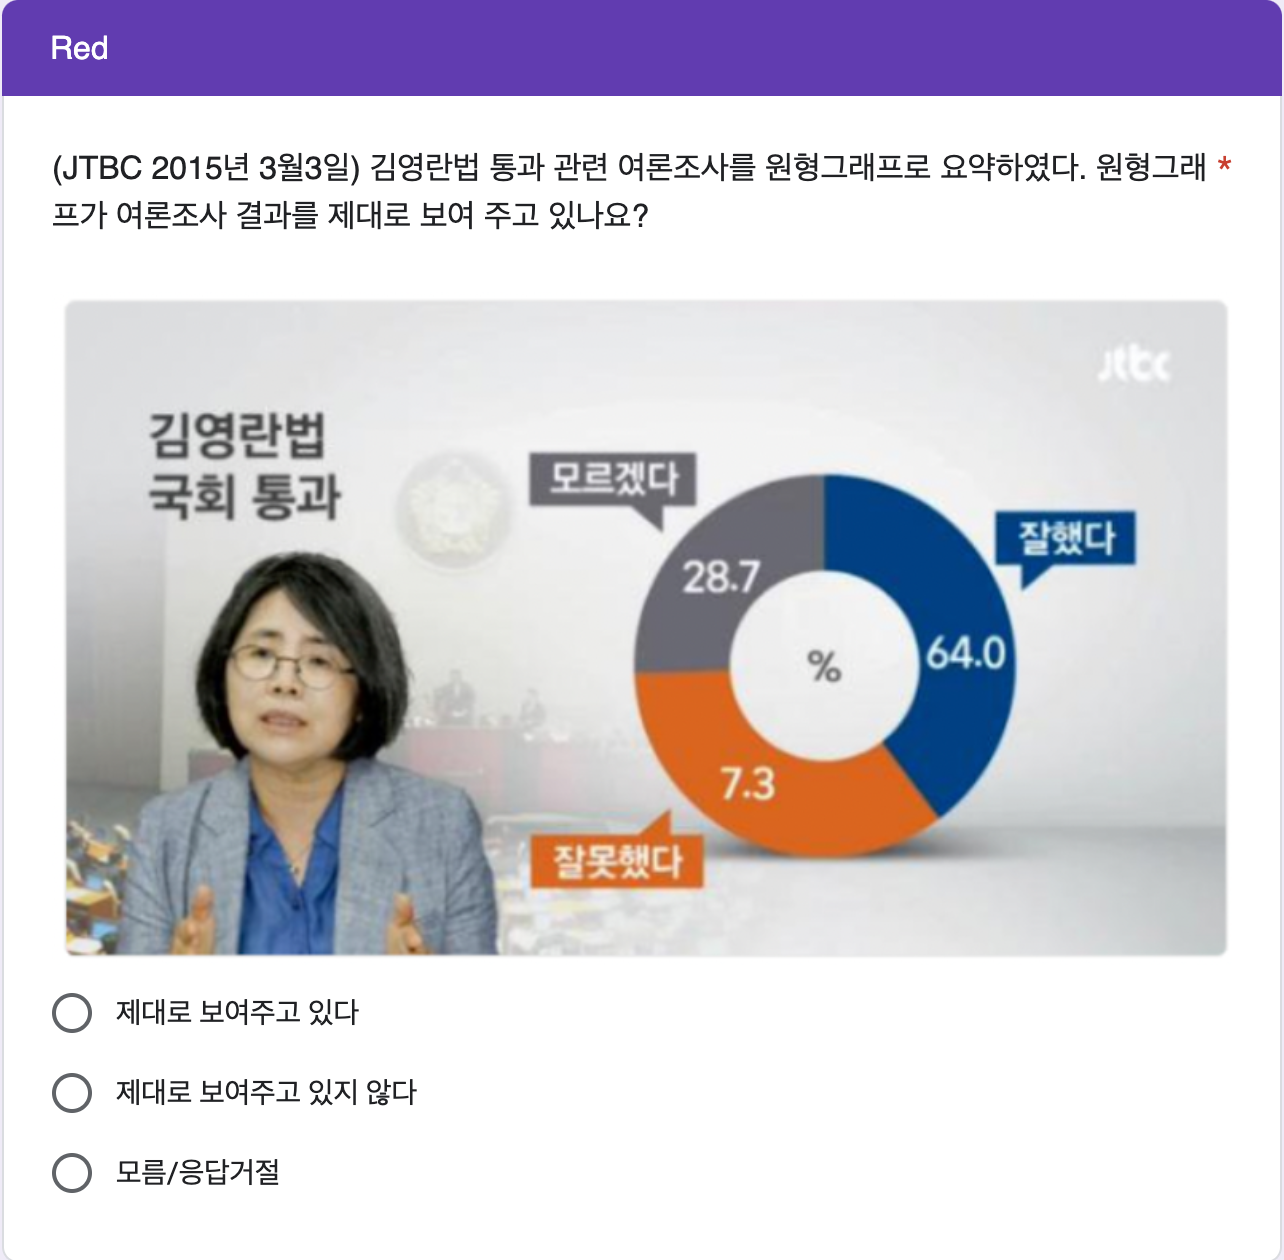
\includegraphics[width=0.67\linewidth]{./pics/Quiz240308_Q7_Red}

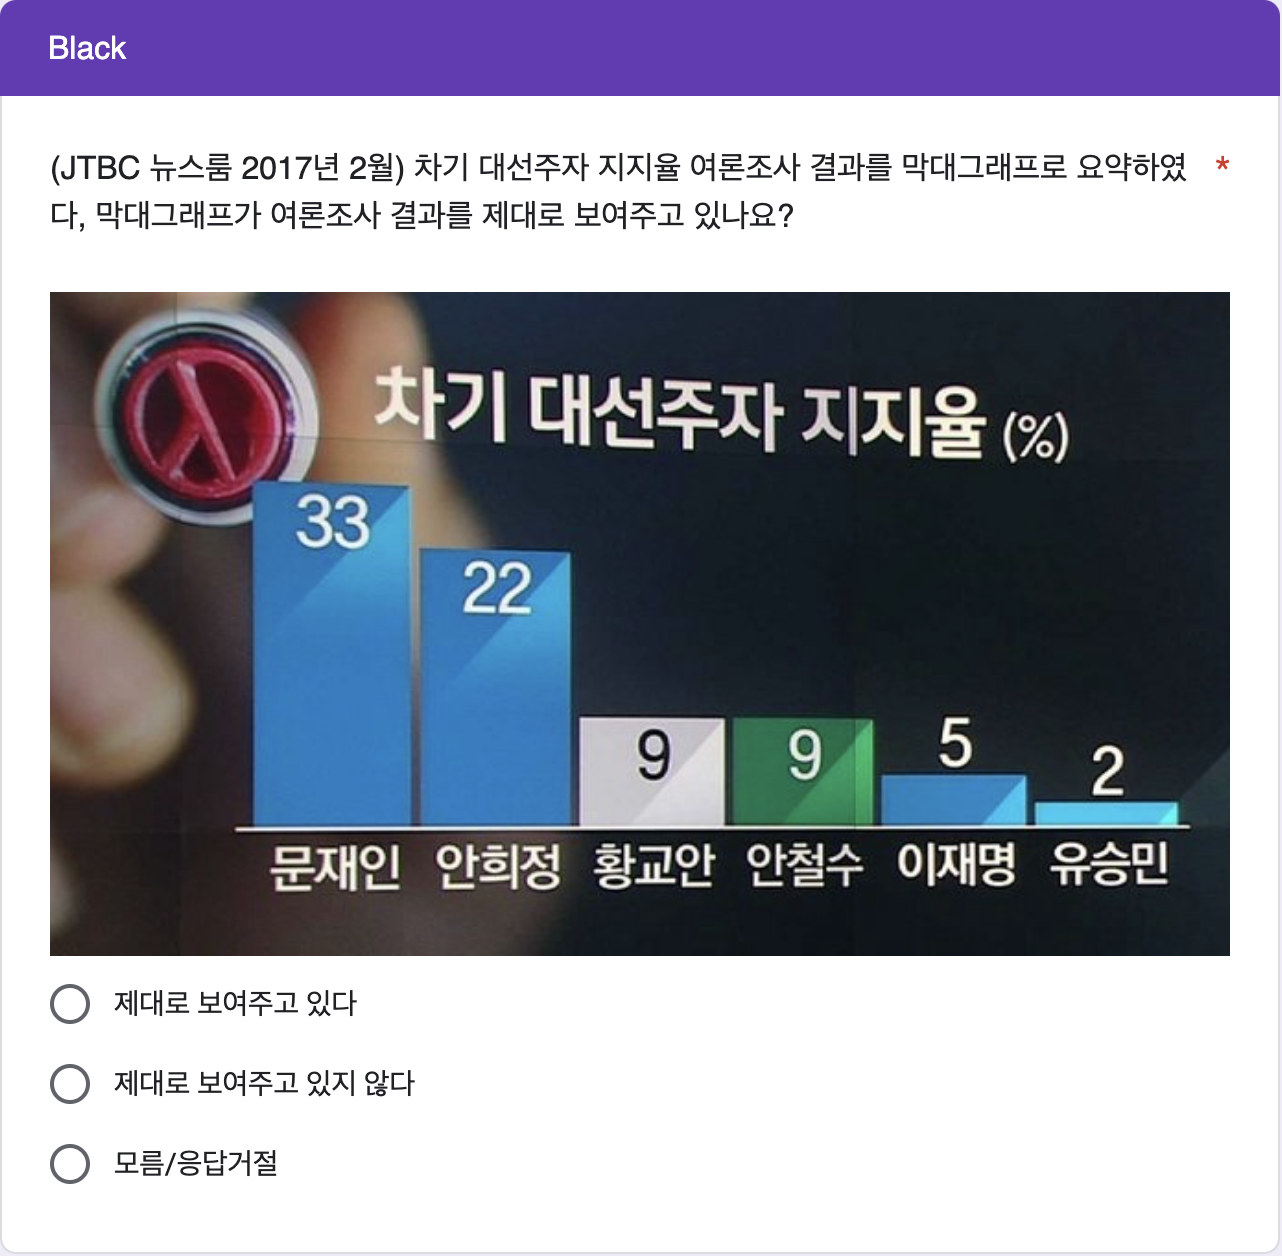
\includegraphics[width=0.67\linewidth]{./pics/Quiz240308_Q7_Black}

\subsection{집계표}\label{uxc9d1uxacc4uxd45c}

\begin{longtable}[]{@{}
  >{\raggedright\arraybackslash}p{(\linewidth - 8\tabcolsep) * \real{0.3048}}
  >{\centering\arraybackslash}p{(\linewidth - 8\tabcolsep) * \real{0.2190}}
  >{\centering\arraybackslash}p{(\linewidth - 8\tabcolsep) * \real{0.2667}}
  >{\centering\arraybackslash}p{(\linewidth - 8\tabcolsep) * \real{0.1524}}
  >{\centering\arraybackslash}p{(\linewidth - 8\tabcolsep) * \real{0.0571}}@{}}
\toprule\noalign{}
\begin{minipage}[b]{\linewidth}\raggedright
~
\end{minipage} & \begin{minipage}[b]{\linewidth}\centering
제대로 보여주고 있다
\end{minipage} & \begin{minipage}[b]{\linewidth}\centering
제대로 보여주고 있지 않다
\end{minipage} & \begin{minipage}[b]{\linewidth}\centering
모름/응답거절
\end{minipage} & \begin{minipage}[b]{\linewidth}\centering
계
\end{minipage} \\
\midrule\noalign{}
\endhead
\bottomrule\noalign{}
\endlastfoot
\textbf{Red(김영란법 국회통과)} & 65 & 180 & 37 & 282 \\
\textbf{Black(고위공직자 범죄수사처
설립)} & 100 & 119 & 62 & 281 \\
\textbf{계} & 165 & 299 & 99 & 563 \\
\end{longtable}

\begin{longtable}[]{@{}
  >{\raggedleft\arraybackslash}p{(\linewidth - 4\tabcolsep) * \real{0.2361}}
  >{\raggedleft\arraybackslash}p{(\linewidth - 4\tabcolsep) * \real{0.0694}}
  >{\raggedleft\arraybackslash}p{(\linewidth - 4\tabcolsep) * \real{0.2500}}@{}}
\caption{Pearson's Chi-squared test: \texttt{.}}\tabularnewline
\toprule\noalign{}
\begin{minipage}[b]{\linewidth}\raggedleft
Test statistic
\end{minipage} & \begin{minipage}[b]{\linewidth}\raggedleft
df
\end{minipage} & \begin{minipage}[b]{\linewidth}\raggedleft
P value
\end{minipage} \\
\midrule\noalign{}
\endfirsthead
\toprule\noalign{}
\begin{minipage}[b]{\linewidth}\raggedleft
Test statistic
\end{minipage} & \begin{minipage}[b]{\linewidth}\raggedleft
df
\end{minipage} & \begin{minipage}[b]{\linewidth}\raggedleft
P value
\end{minipage} \\
\midrule\noalign{}
\endhead
\bottomrule\noalign{}
\endlastfoot
26.18 & 2 & 2.065e-06 * * * \\
\end{longtable}

Q7의 Red에는 김영란법 국회통과에 대한 여론조사 결과를 원형그래프로 나타내었는데 잘했다(64\%), 잘못했다(7.3\%), 모르겠다(28.7\%)의 각도를 데이터와 전혀 맞지 않게 왜곡하여 마치 잘했다와 잘못했다의 비율이 거의 대등한 것처럼 각도를 조정하였습니다.

282명이 응답한 가운데 65명이 결과를 ``제대로 보여주고 있다''는 반응을 보이고, 180명이 결과를 ``제대로 보여주고 있지 않다''는 반응을 보입니다.

Black은 2017년 대선의 대선주자 여론조사에서 33\%의 지지율을 기록한 문재인 예비후보와 22\%의 지지율을 기록한 안희정 예비후보의 지지율 막대가 거의 비슷한 것처럼 왜곡하였습니다.

281명이 응답한 가운데 100명이 여론조사 결과를 ''
제대로 보여주고 있다''는 반응을 보이고, 119명이 여론조사 결과를 ``제대로 보여주고 있지 않다''는 반응을 보입니다.

그리고 ``모름/무응답''에 답한 인원은 Red에 37명, Black 에 62명이 었습니다.

카이제곱 테스트는 이와 같은 상황에서 원형그래프를 왜곡할 떄와 막대그래프를 왜곡할 때 인식의 차이가 통계적으로 유의하다는 것을 보여 줍니다.

카이제곱 통계량은 26.180, 자유도는 2, p-value 는 2.1e-06(으)로
그래프의 유형에 따라 눈속임의 인식에 통계적으로 유의한 차이가 관찰된다는 것을 보여줍니다.

여기서 그래프의 유형이 눈속임의 인식에 차이를 주지 않는다고 가정합니다.

랜덤화의 효과로 Red, Black 의 응답은 닮게 마련입니다.

즉, 통계적으로 유의한 차이를 보이지 않게 됩니다.

그러나 실제로 관찰된 카이제곱 통계값의 P-value 는 0.05보다 매우 작은 값입니다.

따라서, 그래프의 유형이 눈속임의 인식에 영향을 끼치지 않는다는 가정은 잘못된 것이죠.

이러한 논증 방식을 귀류법이라고 합니다.

\subsection{\% 비교}\label{uxbe44uxad50}

\begin{longtable}[]{@{}
  >{\raggedright\arraybackslash}p{(\linewidth - 8\tabcolsep) * \real{0.2991}}
  >{\centering\arraybackslash}p{(\linewidth - 8\tabcolsep) * \real{0.2150}}
  >{\centering\arraybackslash}p{(\linewidth - 8\tabcolsep) * \real{0.2617}}
  >{\centering\arraybackslash}p{(\linewidth - 8\tabcolsep) * \real{0.1495}}
  >{\centering\arraybackslash}p{(\linewidth - 8\tabcolsep) * \real{0.0748}}@{}}
\toprule\noalign{}
\begin{minipage}[b]{\linewidth}\raggedright
~
\end{minipage} & \begin{minipage}[b]{\linewidth}\centering
제대로 보여주고 있다
\end{minipage} & \begin{minipage}[b]{\linewidth}\centering
제대로 보여주고 있지 않다
\end{minipage} & \begin{minipage}[b]{\linewidth}\centering
모름/응답거절
\end{minipage} & \begin{minipage}[b]{\linewidth}\centering
계
\end{minipage} \\
\midrule\noalign{}
\endhead
\bottomrule\noalign{}
\endlastfoot
\textbf{Red(김영란법 국회통과)} & 23.0 & 63.8 & 13.1 & 100.0 \\
\textbf{Black(고위공직자 범죄수사처
설립)} & 35.6 & 42.3 & 22.1 & 100.0 \\
\end{longtable}

원형그래프의 각도를 왜곡한 Red에서 여론조사 결과를 ``제대로 보여주고 있다''고 응답하는 사람들의 백분율, 23.0(\%)은 ``제대로 보여주고 있지 않다''고 응답하는 사람들의 백분율, 63.8(\%) 보다 매우 낮습니다.

반면 막대그래프의 높이를 왜곡한 Black에서 여론조사 결과를 ``제대로 보여주고 있다''고 응답하는 사람들의 백분율, 35.6(\%)은 ``제대로 보여주고 있지 않다''고 응답하는 사람들의 백분율, 42.3(\%) 보다 적습니다.

원형그래프에서 눈속임을 지각하는 백분율이 막대그래프에서 눈속임을 지각하는 백분율보다 훨씬 높게 나타나고 있습니다.

원형그래프의 각도를 속이느냐, 막대그래프의 높이를 속이느냐에 따라 반응이 달라진다는 것을 잘 알 수 있습니다.

\subsection{Mosaic Plot}\label{mosaic-plot-2}

\pandocbounded{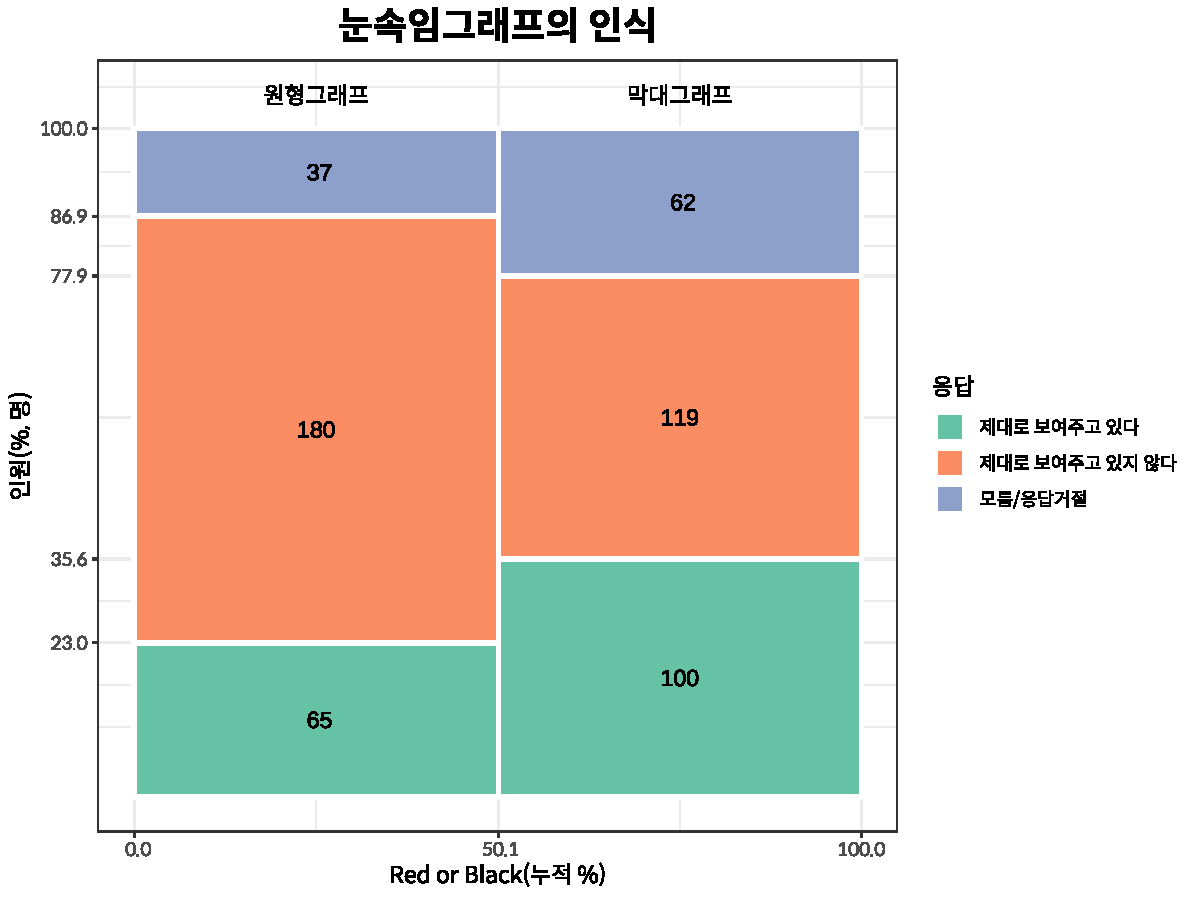
\includegraphics[keepaspectratio]{Quiz_report_2025_files/figure-latex/unnamed-chunk-37-1.pdf}}

Mosaic Plot 은 이 집계결과를 시각적으로 잘 보여줍니다.

원형그래프의 각도를 왜곡한 Red 에서 여론조사 결과를 ``제대로 보여주고 있다''고 응답한 백분율이 매우 낮고, 막대그래프의 높이를 왜곡한 Black 에서 여론조사 결과를 ``제대로 보여주고 있다''고 응답한 백분율은 상대적으로 덜 낮은 것을 시각적으로 알 수 있습니다.

\section{마감 시간으로부터 제출 시간의 분포}\label{uxb9c8uxac10-uxc2dcuxac04uxc73cuxb85cuxbd80uxd130-uxc81cuxcd9c-uxc2dcuxac04uxc758-uxbd84uxd3ec-1}

\subsection{분포표}\label{uxbd84uxd3ecuxd45c-1}

\begin{longtable}[]{@{}
  >{\raggedright\arraybackslash}p{(\linewidth - 30\tabcolsep) * \real{0.1121}}
  >{\centering\arraybackslash}p{(\linewidth - 30\tabcolsep) * \real{0.0654}}
  >{\centering\arraybackslash}p{(\linewidth - 30\tabcolsep) * \real{0.0654}}
  >{\centering\arraybackslash}p{(\linewidth - 30\tabcolsep) * \real{0.0654}}
  >{\centering\arraybackslash}p{(\linewidth - 30\tabcolsep) * \real{0.0654}}
  >{\centering\arraybackslash}p{(\linewidth - 30\tabcolsep) * \real{0.0654}}
  >{\centering\arraybackslash}p{(\linewidth - 30\tabcolsep) * \real{0.0561}}
  >{\centering\arraybackslash}p{(\linewidth - 30\tabcolsep) * \real{0.0561}}
  >{\centering\arraybackslash}p{(\linewidth - 30\tabcolsep) * \real{0.0561}}
  >{\centering\arraybackslash}p{(\linewidth - 30\tabcolsep) * \real{0.0561}}
  >{\centering\arraybackslash}p{(\linewidth - 30\tabcolsep) * \real{0.0561}}
  >{\centering\arraybackslash}p{(\linewidth - 30\tabcolsep) * \real{0.0561}}
  >{\centering\arraybackslash}p{(\linewidth - 30\tabcolsep) * \real{0.0561}}
  >{\centering\arraybackslash}p{(\linewidth - 30\tabcolsep) * \real{0.0561}}
  >{\centering\arraybackslash}p{(\linewidth - 30\tabcolsep) * \real{0.0561}}
  >{\centering\arraybackslash}p{(\linewidth - 30\tabcolsep) * \real{0.0561}}@{}}
\caption{일 단위}\tabularnewline
\toprule\noalign{}
\begin{minipage}[b]{\linewidth}\raggedright
~
\end{minipage} & \begin{minipage}[b]{\linewidth}\centering
14일
\end{minipage} & \begin{minipage}[b]{\linewidth}\centering
13일
\end{minipage} & \begin{minipage}[b]{\linewidth}\centering
12일
\end{minipage} & \begin{minipage}[b]{\linewidth}\centering
11일
\end{minipage} & \begin{minipage}[b]{\linewidth}\centering
10일
\end{minipage} & \begin{minipage}[b]{\linewidth}\centering
9일
\end{minipage} & \begin{minipage}[b]{\linewidth}\centering
8일
\end{minipage} & \begin{minipage}[b]{\linewidth}\centering
7일
\end{minipage} & \begin{minipage}[b]{\linewidth}\centering
6일
\end{minipage} & \begin{minipage}[b]{\linewidth}\centering
5일
\end{minipage} & \begin{minipage}[b]{\linewidth}\centering
4일
\end{minipage} & \begin{minipage}[b]{\linewidth}\centering
3일
\end{minipage} & \begin{minipage}[b]{\linewidth}\centering
2일
\end{minipage} & \begin{minipage}[b]{\linewidth}\centering
1일
\end{minipage} & \begin{minipage}[b]{\linewidth}\centering
계
\end{minipage} \\
\midrule\noalign{}
\endfirsthead
\toprule\noalign{}
\begin{minipage}[b]{\linewidth}\raggedright
~
\end{minipage} & \begin{minipage}[b]{\linewidth}\centering
14일
\end{minipage} & \begin{minipage}[b]{\linewidth}\centering
13일
\end{minipage} & \begin{minipage}[b]{\linewidth}\centering
12일
\end{minipage} & \begin{minipage}[b]{\linewidth}\centering
11일
\end{minipage} & \begin{minipage}[b]{\linewidth}\centering
10일
\end{minipage} & \begin{minipage}[b]{\linewidth}\centering
9일
\end{minipage} & \begin{minipage}[b]{\linewidth}\centering
8일
\end{minipage} & \begin{minipage}[b]{\linewidth}\centering
7일
\end{minipage} & \begin{minipage}[b]{\linewidth}\centering
6일
\end{minipage} & \begin{minipage}[b]{\linewidth}\centering
5일
\end{minipage} & \begin{minipage}[b]{\linewidth}\centering
4일
\end{minipage} & \begin{minipage}[b]{\linewidth}\centering
3일
\end{minipage} & \begin{minipage}[b]{\linewidth}\centering
2일
\end{minipage} & \begin{minipage}[b]{\linewidth}\centering
1일
\end{minipage} & \begin{minipage}[b]{\linewidth}\centering
계
\end{minipage} \\
\midrule\noalign{}
\endhead
\bottomrule\noalign{}
\endlastfoot
\textbf{Red} & 52 & 17 & 9 & 6 & 12 & 8 & 12 & 51 & 20 & 13 & 21 & 13 & 21 & 27 & 282 \\
\textbf{Black} & 59 & 11 & 11 & 3 & 6 & 7 & 9 & 43 & 19 & 18 & 20 & 21 & 26 & 28 & 281 \\
\textbf{계} & 111 & 28 & 20 & 9 & 18 & 15 & 21 & 94 & 39 & 31 & 41 & 34 & 47 & 55 & 563 \\
\end{longtable}

분포표로부터 두 가지 문제를 살펴보겠습니다.

첫째, 날마다 고르게 제출하는가?

둘째, Red, Black 간에 통계적으로 유의한 차이가 있는가?

각 문제를 살펴보기 위해서는 분포표의 일부분을 대상으로 카이제곱 테스트를 수행합니다.

\subsection{날마다 고르게 제출하는가?}\label{uxb0a0uxb9c8uxb2e4-uxace0uxb974uxac8c-uxc81cuxcd9cuxd558uxb294uxac00-1}

\begin{longtable}[]{@{}
  >{\centering\arraybackslash}p{(\linewidth - 26\tabcolsep) * \real{0.0787}}
  >{\centering\arraybackslash}p{(\linewidth - 26\tabcolsep) * \real{0.0787}}
  >{\centering\arraybackslash}p{(\linewidth - 26\tabcolsep) * \real{0.0787}}
  >{\centering\arraybackslash}p{(\linewidth - 26\tabcolsep) * \real{0.0787}}
  >{\centering\arraybackslash}p{(\linewidth - 26\tabcolsep) * \real{0.0787}}
  >{\centering\arraybackslash}p{(\linewidth - 26\tabcolsep) * \real{0.0674}}
  >{\centering\arraybackslash}p{(\linewidth - 26\tabcolsep) * \real{0.0674}}
  >{\centering\arraybackslash}p{(\linewidth - 26\tabcolsep) * \real{0.0674}}
  >{\centering\arraybackslash}p{(\linewidth - 26\tabcolsep) * \real{0.0674}}
  >{\centering\arraybackslash}p{(\linewidth - 26\tabcolsep) * \real{0.0674}}
  >{\centering\arraybackslash}p{(\linewidth - 26\tabcolsep) * \real{0.0674}}
  >{\centering\arraybackslash}p{(\linewidth - 26\tabcolsep) * \real{0.0674}}
  >{\centering\arraybackslash}p{(\linewidth - 26\tabcolsep) * \real{0.0674}}
  >{\centering\arraybackslash}p{(\linewidth - 26\tabcolsep) * \real{0.0674}}@{}}
\toprule\noalign{}
\begin{minipage}[b]{\linewidth}\centering
14일
\end{minipage} & \begin{minipage}[b]{\linewidth}\centering
13일
\end{minipage} & \begin{minipage}[b]{\linewidth}\centering
12일
\end{minipage} & \begin{minipage}[b]{\linewidth}\centering
11일
\end{minipage} & \begin{minipage}[b]{\linewidth}\centering
10일
\end{minipage} & \begin{minipage}[b]{\linewidth}\centering
9일
\end{minipage} & \begin{minipage}[b]{\linewidth}\centering
8일
\end{minipage} & \begin{minipage}[b]{\linewidth}\centering
7일
\end{minipage} & \begin{minipage}[b]{\linewidth}\centering
6일
\end{minipage} & \begin{minipage}[b]{\linewidth}\centering
5일
\end{minipage} & \begin{minipage}[b]{\linewidth}\centering
4일
\end{minipage} & \begin{minipage}[b]{\linewidth}\centering
3일
\end{minipage} & \begin{minipage}[b]{\linewidth}\centering
2일
\end{minipage} & \begin{minipage}[b]{\linewidth}\centering
1일
\end{minipage} \\
\midrule\noalign{}
\endhead
\bottomrule\noalign{}
\endlastfoot
111 & 28 & 20 & 9 & 18 & 15 & 21 & 94 & 39 & 31 & 41 & 34 & 47 & 55 \\
\end{longtable}

\begin{longtable}[]{@{}
  >{\raggedleft\arraybackslash}p{(\linewidth - 4\tabcolsep) * \real{0.2361}}
  >{\raggedleft\arraybackslash}p{(\linewidth - 4\tabcolsep) * \real{0.0694}}
  >{\raggedleft\arraybackslash}p{(\linewidth - 4\tabcolsep) * \real{0.2500}}@{}}
\caption{Chi-squared test for given probabilities: \texttt{.}}\tabularnewline
\toprule\noalign{}
\begin{minipage}[b]{\linewidth}\raggedleft
Test statistic
\end{minipage} & \begin{minipage}[b]{\linewidth}\raggedleft
df
\end{minipage} & \begin{minipage}[b]{\linewidth}\raggedleft
P value
\end{minipage} \\
\midrule\noalign{}
\endfirsthead
\toprule\noalign{}
\begin{minipage}[b]{\linewidth}\raggedleft
Test statistic
\end{minipage} & \begin{minipage}[b]{\linewidth}\raggedleft
df
\end{minipage} & \begin{minipage}[b]{\linewidth}\raggedleft
P value
\end{minipage} \\
\midrule\noalign{}
\endhead
\bottomrule\noalign{}
\endlastfoot
281.6 & 13 & 1.685e-52 * * * \\
\end{longtable}

날마다 고르게 제출하는지 알아 보았습니다.

분포표의 ``계''행에서 '계'열을 제외하고 카이제곱테스트를 수행합니다.

분포표 만으로도 쉽게 파악할 수 있지만 카이제곱테스트가 명확히 해 줍니다.

카이제곱 통계량은 281.60, 자유도는 13.00, p-value 는 1.7e-52 이므로 결코 고르게 제출한다고 말할 수 없겠습니다.

막대그래프로 살펴 보겠습니다.

\subsection{막대그래프}\label{uxb9c9uxb300uxadf8uxb798uxd504-1}

\pandocbounded{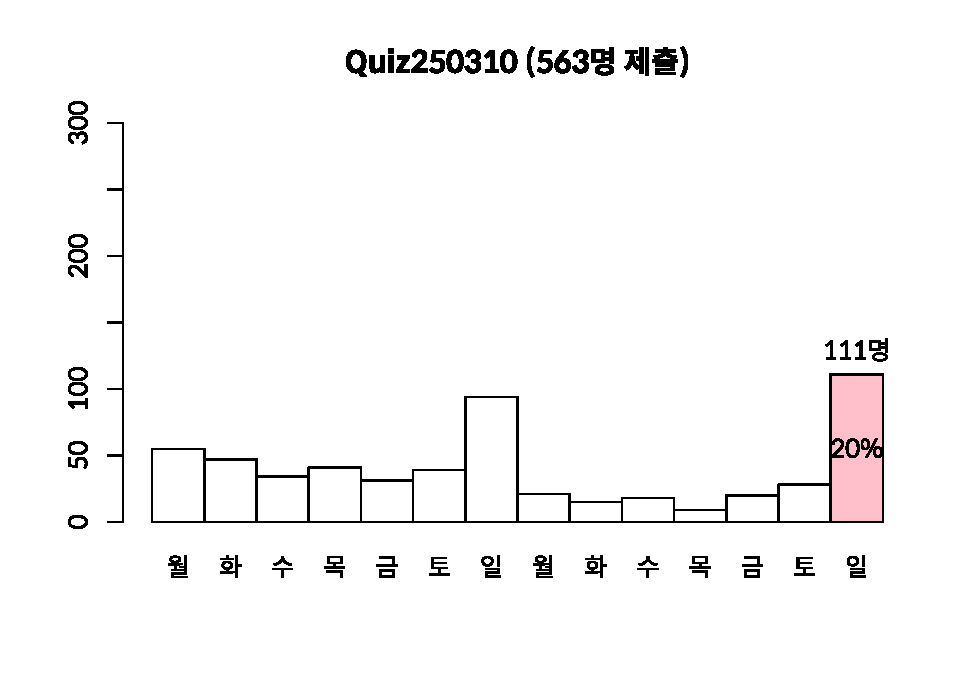
\includegraphics[keepaspectratio]{Quiz_report_2025_files/figure-latex/unnamed-chunk-40-1.pdf}}

막대그래프는 총 제출인원 563(명) 중에 111(명), 20(\%)가 마감일에 몰리는 것을 명확히 보여주고 있습니다.

\subsection{Red, Black 간에 닮았는가?}\label{red-black-uxac04uxc5d0-uxb2eeuxc558uxb294uxac00-1}

\begin{longtable}[]{@{}
  >{\raggedright\arraybackslash}p{(\linewidth - 28\tabcolsep) * \real{0.1188}}
  >{\centering\arraybackslash}p{(\linewidth - 28\tabcolsep) * \real{0.0693}}
  >{\centering\arraybackslash}p{(\linewidth - 28\tabcolsep) * \real{0.0693}}
  >{\centering\arraybackslash}p{(\linewidth - 28\tabcolsep) * \real{0.0693}}
  >{\centering\arraybackslash}p{(\linewidth - 28\tabcolsep) * \real{0.0693}}
  >{\centering\arraybackslash}p{(\linewidth - 28\tabcolsep) * \real{0.0693}}
  >{\centering\arraybackslash}p{(\linewidth - 28\tabcolsep) * \real{0.0594}}
  >{\centering\arraybackslash}p{(\linewidth - 28\tabcolsep) * \real{0.0594}}
  >{\centering\arraybackslash}p{(\linewidth - 28\tabcolsep) * \real{0.0594}}
  >{\centering\arraybackslash}p{(\linewidth - 28\tabcolsep) * \real{0.0594}}
  >{\centering\arraybackslash}p{(\linewidth - 28\tabcolsep) * \real{0.0594}}
  >{\centering\arraybackslash}p{(\linewidth - 28\tabcolsep) * \real{0.0594}}
  >{\centering\arraybackslash}p{(\linewidth - 28\tabcolsep) * \real{0.0594}}
  >{\centering\arraybackslash}p{(\linewidth - 28\tabcolsep) * \real{0.0594}}
  >{\centering\arraybackslash}p{(\linewidth - 28\tabcolsep) * \real{0.0594}}@{}}
\toprule\noalign{}
\begin{minipage}[b]{\linewidth}\raggedright
~
\end{minipage} & \begin{minipage}[b]{\linewidth}\centering
14일
\end{minipage} & \begin{minipage}[b]{\linewidth}\centering
13일
\end{minipage} & \begin{minipage}[b]{\linewidth}\centering
12일
\end{minipage} & \begin{minipage}[b]{\linewidth}\centering
11일
\end{minipage} & \begin{minipage}[b]{\linewidth}\centering
10일
\end{minipage} & \begin{minipage}[b]{\linewidth}\centering
9일
\end{minipage} & \begin{minipage}[b]{\linewidth}\centering
8일
\end{minipage} & \begin{minipage}[b]{\linewidth}\centering
7일
\end{minipage} & \begin{minipage}[b]{\linewidth}\centering
6일
\end{minipage} & \begin{minipage}[b]{\linewidth}\centering
5일
\end{minipage} & \begin{minipage}[b]{\linewidth}\centering
4일
\end{minipage} & \begin{minipage}[b]{\linewidth}\centering
3일
\end{minipage} & \begin{minipage}[b]{\linewidth}\centering
2일
\end{minipage} & \begin{minipage}[b]{\linewidth}\centering
1일
\end{minipage} \\
\midrule\noalign{}
\endhead
\bottomrule\noalign{}
\endlastfoot
\textbf{Red} & 52 & 17 & 9 & 6 & 12 & 8 & 12 & 51 & 20 & 13 & 21 & 13 & 21 & 27 \\
\textbf{Black} & 59 & 11 & 11 & 3 & 6 & 7 & 9 & 43 & 19 & 18 & 20 & 21 & 26 & 28 \\
\end{longtable}

\begin{longtable}[]{@{}
  >{\raggedleft\arraybackslash}p{(\linewidth - 4\tabcolsep) * \real{0.2361}}
  >{\raggedleft\arraybackslash}p{(\linewidth - 4\tabcolsep) * \real{0.0694}}
  >{\raggedleft\arraybackslash}p{(\linewidth - 4\tabcolsep) * \real{0.1389}}@{}}
\caption{Pearson's Chi-squared test: \texttt{.}}\tabularnewline
\toprule\noalign{}
\begin{minipage}[b]{\linewidth}\raggedleft
Test statistic
\end{minipage} & \begin{minipage}[b]{\linewidth}\raggedleft
df
\end{minipage} & \begin{minipage}[b]{\linewidth}\raggedleft
P value
\end{minipage} \\
\midrule\noalign{}
\endfirsthead
\toprule\noalign{}
\begin{minipage}[b]{\linewidth}\raggedleft
Test statistic
\end{minipage} & \begin{minipage}[b]{\linewidth}\raggedleft
df
\end{minipage} & \begin{minipage}[b]{\linewidth}\raggedleft
P value
\end{minipage} \\
\midrule\noalign{}
\endhead
\bottomrule\noalign{}
\endlastfoot
9.39 & 13 & 0.7429 \\
\end{longtable}

제출시간의 분포가 Red, Black 간에 닮았는지 알아 보았습니다.

이번에는 분포표의 첫번째와 두번째 행, '계'열을 제외한 나머지 열에 대해서 카이제곱테스트를 수행합니다.

카이제곱 통계량은 9.390, 자유도는 13, p-value 는 0.7429 이므로 제출 시간의 분포는 Red, Black 간에 통계적으로 유의한 차이가 관찰되지 않습니다.

이 사실을 Mosaic Plot 을 이용하여 시각적으로 살펴보겠습니다.

닮았다고 느껴지나요?

\subsection{Mosaic Plot}\label{mosaic-plot-3}

\pandocbounded{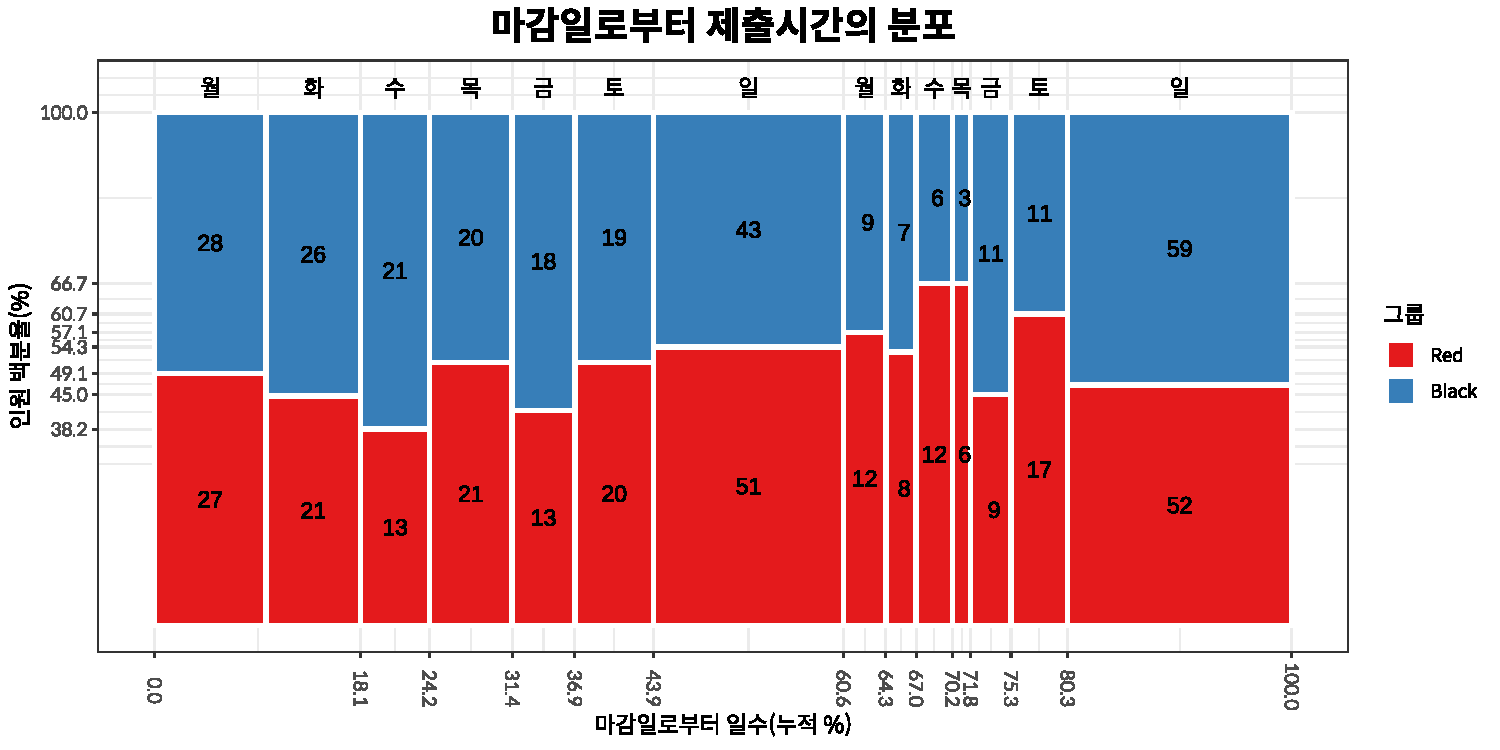
\includegraphics[keepaspectratio]{Quiz_report_2025_files/figure-latex/unnamed-chunk-42-1.pdf}}

\chapter{3주차 데이터 실험 집계}\label{uxc8fcuxcc28-uxb370uxc774uxd130-uxc2e4uxd5d8-uxc9d1uxacc4-2}

\section{실험의 목적}\label{uxc2e4uxd5d8uxc758-uxbaa9uxc801-2}

3주차 구글 예습 설문지 집계결과를 분석합니다.

Q1\textasciitilde Q6에서는 랜덤화의 효과로 Red, Black 이 얼마나 닮았는지 알아봅니다.

Q7에서는 같은 사안에 대해서 질문 안에 편향된 정보를 담아 넣었을 때 Red, Black 의 응답이 어떻게 달라지는 지 알아봅니다.

끝으로 제출시간의 분포가 날마다 고른지, Red, Black 간에는 닮았는지 알아봅니다.

\subsection{Red, Black을 잘못 표시한 사람들}\label{red-blackuxc744-uxc798uxbabb-uxd45cuxc2dcuxd55c-uxc0acuxb78cuxb4e4-2}

\begin{longtable}[]{@{}
  >{\raggedright\arraybackslash}p{(\linewidth - 4\tabcolsep) * \real{0.3611}}
  >{\centering\arraybackslash}p{(\linewidth - 4\tabcolsep) * \real{0.2778}}
  >{\centering\arraybackslash}p{(\linewidth - 4\tabcolsep) * \real{0.3056}}@{}}
\toprule\noalign{}
\begin{minipage}[b]{\linewidth}\raggedright
~
\end{minipage} & \begin{minipage}[b]{\linewidth}\centering
Red(구글예습퀴즈)
\end{minipage} & \begin{minipage}[b]{\linewidth}\centering
Black(구글예습퀴즈)
\end{minipage} \\
\midrule\noalign{}
\endhead
\bottomrule\noalign{}
\endlastfoot
\textbf{Red(랜덤화출석부)} & 273 & 5 \\
\textbf{Black(랜덤화출석부)} & 4 & 271 \\
\textbf{계} & 277 & 276 \\
\end{longtable}

랜덤화출석부에 있는 Red, Black 과 실제 구글설문에 올린 Red, Black 이 다른 사람들의 수효는 9명입니다.

Red를 Black 이라고 한 사람이 5명, Black 을 Red 라고 한 사람이 4명입니다.

두 가지 방법으로 분석합니다.

우선 Red, Black 을 잘못 선택한 9명을 랜덤하게 둘로 나누면 어느 한 쪽 집단에 들어갈 기대인원은 9명을 둘로 나눈 4.5(명)이고, 표준오차는 9의 제곱근에 1/2을 곱해 준 1.5명이 됩니다.

실제로 Red를 Black 이라고 한 사람수, 5명이나 Black 을 Red 라고 한 사람수, 4명은 기대인원으로부터 표준오차 범위 안에 아주 잘 들어갑니다.

두 번째 분석 방법은 확률을 계산해 보는 것입니다.

Red, Black 을 잘못 선택한 9명을 랜덤하게 둘로 나눌 때, 실제로 관찰된 5명 이상이나 4명이하로 잘못 선택한 사람수가 나올 가능성은 얼마나 되는가 입니다.

이 경우 공평한 동전던지기를 확률 법칙으로 표현한 이항분포로부터 계산할 수 있습니다.

시행횟수가 9이고 한 번 시행에서 성공확률이 1/2 인 이항분포에서 성공횟수가 4이하이거나 5이상을 관찰할 확률은 1입니다.

공평한 동전 던지기에서 앞면이 4개 이하 나오는 확률은 5개 이상 나오는 확률과 같기 때문에 사실상 한쪽만 계산해서 2배 해 주면 됩니다.

이 값을 p-value 라고 하는데, p-value가 0.05보다 작을 때 \textbf{통계적으로 유의한 차이를 관찰}하였다고 말합니다.

즉, 공평한 동전을 던지는 것과 같은 과정이라고 가정하였을 때 실제로 관찰된 값들이 가정으로부터 얼마나 떨어져 있는지를 표현한 것입니다.

0.05, 즉 1/20은 이런 실험을 스무 번 정도 반복하면 1번 나올 정도로 드문 사건을 의미합니다.

즉 가정이 타당하다면 나오기 힘든 결과라는 것입니다.

그런데 Red, Black 을 잘못 표시한 사람들의 분포에서 관찰된 p-value 는 0.05와는 비교도 안될 정도로 큰 값입니다.

따라서 두 집단이 랜덤화 효과가 작동하여 \textbf{통계적으로 유의한 차이를 보이지 않는다}고 할 수 있습니다.

\subsection{응답인원의 Red, Black}\label{uxc751uxb2f5uxc778uxc6d0uxc758-red-black-2}

Red 로 응답한 인원은 277명, Black 에 응답한 인원은 276명입니다.

전체 응답인원 553 명을 랜덤하게 둘로 나눌 때 어느 한 쪽의 기대인원은 전체 응답인원의 절반인 276.5명이고, 표준오차는 전체 응답인원의 제곱근에 1/2을 곱해 준 11.8 명입니다.

따라서 Red, Black 각 그룹에 관찰된 인원은 기대인원으로부터 표준오차 범위 안에 들어갑니다.

\section{Q1. 국세와 지방세 비중}\label{q1.-uxad6duxc138uxc640-uxc9c0uxbc29uxc138-uxbe44uxc911}


\includegraphics[width=0.75\linewidth]{./pics/Quiz230315_Q1}

\subsection{국세와 지방세 비중(집계표)}\label{uxad6duxc138uxc640-uxc9c0uxbc29uxc138-uxbe44uxc911uxc9d1uxacc4uxd45c}

\begin{longtable}[]{@{}
  >{\raggedright\arraybackslash}p{(\linewidth - 12\tabcolsep) * \real{0.1667}}
  >{\raggedleft\arraybackslash}p{(\linewidth - 12\tabcolsep) * \real{0.1111}}
  >{\raggedleft\arraybackslash}p{(\linewidth - 12\tabcolsep) * \real{0.1111}}
  >{\raggedleft\arraybackslash}p{(\linewidth - 12\tabcolsep) * \real{0.1111}}
  >{\raggedleft\arraybackslash}p{(\linewidth - 12\tabcolsep) * \real{0.1111}}
  >{\raggedleft\arraybackslash}p{(\linewidth - 12\tabcolsep) * \real{0.1111}}
  >{\centering\arraybackslash}p{(\linewidth - 12\tabcolsep) * \real{0.1111}}@{}}
\toprule\noalign{}
\begin{minipage}[b]{\linewidth}\raggedright
~
\end{minipage} & \begin{minipage}[b]{\linewidth}\raggedleft
78:22
\end{minipage} & \begin{minipage}[b]{\linewidth}\raggedleft
77:23
\end{minipage} & \begin{minipage}[b]{\linewidth}\raggedleft
76:24
\end{minipage} & \begin{minipage}[b]{\linewidth}\raggedleft
75:25
\end{minipage} & \begin{minipage}[b]{\linewidth}\raggedleft
74:26
\end{minipage} & \begin{minipage}[b]{\linewidth}\centering
계
\end{minipage} \\
\midrule\noalign{}
\endhead
\bottomrule\noalign{}
\endlastfoot
\textbf{Red} & 16 & 35 & 45 & 29 & 152 & 277 \\
\textbf{Black} & 16 & 33 & 55 & 23 & 149 & 276 \\
\textbf{계} & 32 & 68 & 100 & 52 & 301 & 553 \\
\end{longtable}

\begin{longtable}[]{@{}
  >{\raggedleft\arraybackslash}p{(\linewidth - 4\tabcolsep) * \real{0.2361}}
  >{\raggedleft\arraybackslash}p{(\linewidth - 4\tabcolsep) * \real{0.0694}}
  >{\raggedleft\arraybackslash}p{(\linewidth - 4\tabcolsep) * \real{0.1389}}@{}}
\caption{Pearson's Chi-squared test: \texttt{.}}\tabularnewline
\toprule\noalign{}
\begin{minipage}[b]{\linewidth}\raggedleft
Test statistic
\end{minipage} & \begin{minipage}[b]{\linewidth}\raggedleft
df
\end{minipage} & \begin{minipage}[b]{\linewidth}\raggedleft
P value
\end{minipage} \\
\midrule\noalign{}
\endfirsthead
\toprule\noalign{}
\begin{minipage}[b]{\linewidth}\raggedleft
Test statistic
\end{minipage} & \begin{minipage}[b]{\linewidth}\raggedleft
df
\end{minipage} & \begin{minipage}[b]{\linewidth}\raggedleft
P value
\end{minipage} \\
\midrule\noalign{}
\endhead
\bottomrule\noalign{}
\endlastfoot
1.779 & 4 & 0.7763 \\
\end{longtable}

Q1의 집계 결과가 Red, Black 간에 통계적으로 유의한 차이가 있는지 알아보기 위하여 카이제곱 테스트를 수행하였습니다.

그 결과 카이제곱 통계량은 1.78, 자유도는 4 , p-value 는 0.7763이므로 Red, Black 간에 통계적으로 유의한 차이를 보이지 않습니다.

실제로 닮은 게 느껴집니까?

\subsection{국세와 지방세 비중(\%)}\label{uxad6duxc138uxc640-uxc9c0uxbc29uxc138-uxbe44uxc911}

\begin{longtable}[]{@{}
  >{\raggedleft\arraybackslash}p{(\linewidth - 10\tabcolsep) * \real{0.1111}}
  >{\raggedleft\arraybackslash}p{(\linewidth - 10\tabcolsep) * \real{0.1111}}
  >{\raggedleft\arraybackslash}p{(\linewidth - 10\tabcolsep) * \real{0.1111}}
  >{\raggedleft\arraybackslash}p{(\linewidth - 10\tabcolsep) * \real{0.1111}}
  >{\raggedleft\arraybackslash}p{(\linewidth - 10\tabcolsep) * \real{0.1111}}
  >{\centering\arraybackslash}p{(\linewidth - 10\tabcolsep) * \real{0.1111}}@{}}
\toprule\noalign{}
\begin{minipage}[b]{\linewidth}\raggedleft
78:22
\end{minipage} & \begin{minipage}[b]{\linewidth}\raggedleft
77:23
\end{minipage} & \begin{minipage}[b]{\linewidth}\raggedleft
76:24
\end{minipage} & \begin{minipage}[b]{\linewidth}\raggedleft
75:25
\end{minipage} & \begin{minipage}[b]{\linewidth}\raggedleft
74:26
\end{minipage} & \begin{minipage}[b]{\linewidth}\centering
계
\end{minipage} \\
\midrule\noalign{}
\endhead
\bottomrule\noalign{}
\endlastfoot
5.8 & 12.3 & 18.1 & 9.4 & 54.4 & 100.0 \\
\end{longtable}

정답률은 Red, Black 을 합하여 계산하는데, 54.4(\%) 입니다.

\section{Q2. 조세부담률}\label{q2.-uxc870uxc138uxbd80uxb2f4uxb960}


\includegraphics[width=0.75\linewidth]{./pics/Quiz230315_Q2}

\subsection{조세부담률(집계표)}\label{uxc870uxc138uxbd80uxb2f4uxb960uxc9d1uxacc4uxd45c}

\begin{longtable}[]{@{}
  >{\raggedright\arraybackslash}p{(\linewidth - 12\tabcolsep) * \real{0.1667}}
  >{\raggedleft\arraybackslash}p{(\linewidth - 12\tabcolsep) * \real{0.0833}}
  >{\raggedleft\arraybackslash}p{(\linewidth - 12\tabcolsep) * \real{0.0833}}
  >{\raggedleft\arraybackslash}p{(\linewidth - 12\tabcolsep) * \real{0.0833}}
  >{\raggedleft\arraybackslash}p{(\linewidth - 12\tabcolsep) * \real{0.0833}}
  >{\raggedleft\arraybackslash}p{(\linewidth - 12\tabcolsep) * \real{0.0833}}
  >{\centering\arraybackslash}p{(\linewidth - 12\tabcolsep) * \real{0.0833}}@{}}
\toprule\noalign{}
\begin{minipage}[b]{\linewidth}\raggedright
~
\end{minipage} & \begin{minipage}[b]{\linewidth}\raggedleft
10\%
\end{minipage} & \begin{minipage}[b]{\linewidth}\raggedleft
15\%
\end{minipage} & \begin{minipage}[b]{\linewidth}\raggedleft
20\%
\end{minipage} & \begin{minipage}[b]{\linewidth}\raggedleft
25\%
\end{minipage} & \begin{minipage}[b]{\linewidth}\raggedleft
30\%
\end{minipage} & \begin{minipage}[b]{\linewidth}\centering
계
\end{minipage} \\
\midrule\noalign{}
\endhead
\bottomrule\noalign{}
\endlastfoot
\textbf{Red} & 6 & 28 & 223 & 17 & 3 & 277 \\
\textbf{Black} & 7 & 24 & 221 & 19 & 5 & 276 \\
\textbf{계} & 13 & 52 & 444 & 36 & 8 & 553 \\
\end{longtable}

\begin{longtable}[]{@{}
  >{\raggedleft\arraybackslash}p{(\linewidth - 4\tabcolsep) * \real{0.2361}}
  >{\raggedleft\arraybackslash}p{(\linewidth - 4\tabcolsep) * \real{0.0694}}
  >{\raggedleft\arraybackslash}p{(\linewidth - 4\tabcolsep) * \real{0.1389}}@{}}
\caption{Pearson's Chi-squared test: \texttt{.}}\tabularnewline
\toprule\noalign{}
\begin{minipage}[b]{\linewidth}\raggedleft
Test statistic
\end{minipage} & \begin{minipage}[b]{\linewidth}\raggedleft
df
\end{minipage} & \begin{minipage}[b]{\linewidth}\raggedleft
P value
\end{minipage} \\
\midrule\noalign{}
\endfirsthead
\toprule\noalign{}
\begin{minipage}[b]{\linewidth}\raggedleft
Test statistic
\end{minipage} & \begin{minipage}[b]{\linewidth}\raggedleft
df
\end{minipage} & \begin{minipage}[b]{\linewidth}\raggedleft
P value
\end{minipage} \\
\midrule\noalign{}
\endhead
\bottomrule\noalign{}
\endlastfoot
1.003 & 4 & 0.9094 \\
\end{longtable}

Q2의 집계 결과가 Red, Black 간에 통계적으로 유의한 차이가 있는지 알아보기 위하여 카이제곱 테스트를 수행하였습니다.

그 결과 카이제곱 통계량은 1.003, 자유도는 4, p-value 는 0.9094이므로 Red, Black 간에 통계적으로 유의한 차이를 보이지 않습니다.

실제로 닮은 게 느껴집니까?

\subsection{조세부담률(\%)}\label{uxc870uxc138uxbd80uxb2f4uxb960}

\begin{longtable}[]{@{}
  >{\raggedleft\arraybackslash}p{(\linewidth - 10\tabcolsep) * \real{0.0833}}
  >{\raggedleft\arraybackslash}p{(\linewidth - 10\tabcolsep) * \real{0.0833}}
  >{\raggedleft\arraybackslash}p{(\linewidth - 10\tabcolsep) * \real{0.0972}}
  >{\raggedleft\arraybackslash}p{(\linewidth - 10\tabcolsep) * \real{0.0833}}
  >{\raggedleft\arraybackslash}p{(\linewidth - 10\tabcolsep) * \real{0.0833}}
  >{\centering\arraybackslash}p{(\linewidth - 10\tabcolsep) * \real{0.1111}}@{}}
\toprule\noalign{}
\begin{minipage}[b]{\linewidth}\raggedleft
10\%
\end{minipage} & \begin{minipage}[b]{\linewidth}\raggedleft
15\%
\end{minipage} & \begin{minipage}[b]{\linewidth}\raggedleft
20\%
\end{minipage} & \begin{minipage}[b]{\linewidth}\raggedleft
25\%
\end{minipage} & \begin{minipage}[b]{\linewidth}\raggedleft
30\%
\end{minipage} & \begin{minipage}[b]{\linewidth}\centering
계
\end{minipage} \\
\midrule\noalign{}
\endhead
\bottomrule\noalign{}
\endlastfoot
2.4 & 9.4 & 80.3 & 6.5 & 1.4 & 100.0 \\
\end{longtable}

정답률은 Red, Black 을 합하여 계산하는데, 80.3(\%) 입니다.

\section{Q3. OECD 국민부담률}\label{q3.-oecd-uxad6duxbbfcuxbd80uxb2f4uxb960}

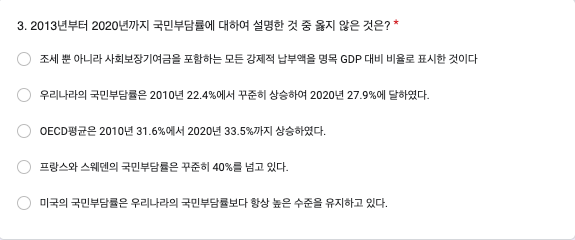
\includegraphics[width=0.75\linewidth]{./pics/Quiz230315_Q3}

\subsection{OECD 국민부담률(집계표)}\label{oecd-uxad6duxbbfcuxbd80uxb2f4uxb960uxc9d1uxacc4uxd45c}

\begin{longtable}[]{@{}
  >{\raggedright\arraybackslash}p{(\linewidth - 12\tabcolsep) * \real{0.0663}}
  >{\centering\arraybackslash}p{(\linewidth - 12\tabcolsep) * \real{0.1823}}
  >{\centering\arraybackslash}p{(\linewidth - 12\tabcolsep) * \real{0.1823}}
  >{\centering\arraybackslash}p{(\linewidth - 12\tabcolsep) * \real{0.1713}}
  >{\centering\arraybackslash}p{(\linewidth - 12\tabcolsep) * \real{0.1823}}
  >{\centering\arraybackslash}p{(\linewidth - 12\tabcolsep) * \real{0.1823}}
  >{\centering\arraybackslash}p{(\linewidth - 12\tabcolsep) * \real{0.0331}}@{}}
\toprule\noalign{}
\begin{minipage}[b]{\linewidth}\raggedright
~
\end{minipage} & \begin{minipage}[b]{\linewidth}\centering
조세 뿐 아니라
사회보장기여금을 포함하는 모든
강제적 납부액을 명목 GDP 대비
비율로 표시한 것이다
\end{minipage} & \begin{minipage}[b]{\linewidth}\centering
우리나라의 국민부담률은 2010년
22.4\%에서 꾸준히 상승하여
2020년 27.9\%에 달하였다.
\end{minipage} & \begin{minipage}[b]{\linewidth}\centering
OECD평균은 2010년 31.6\%에서
2020년 33.5\%까지 상승하였다.
\end{minipage} & \begin{minipage}[b]{\linewidth}\centering
프랑스와 스웨덴의 국민부담률은
꾸준히 40\%를 넘고 있다.
\end{minipage} & \begin{minipage}[b]{\linewidth}\centering
미국의 국민부담률은 우리나라의
국민부담률보다 항상 높은
수준을 유지하고 있다.
\end{minipage} & \begin{minipage}[b]{\linewidth}\centering
계
\end{minipage} \\
\midrule\noalign{}
\endhead
\bottomrule\noalign{}
\endlastfoot
\textbf{Red} & 11 & 40 & 16 & 12 & 198 & 277 \\
\textbf{Black} & 8 & 32 & 18 & 19 & 199 & 276 \\
\textbf{계} & 19 & 72 & 34 & 31 & 397 & 553 \\
\end{longtable}

\begin{longtable}[]{@{}
  >{\raggedleft\arraybackslash}p{(\linewidth - 4\tabcolsep) * \real{0.2361}}
  >{\raggedleft\arraybackslash}p{(\linewidth - 4\tabcolsep) * \real{0.0694}}
  >{\raggedleft\arraybackslash}p{(\linewidth - 4\tabcolsep) * \real{0.1389}}@{}}
\caption{Pearson's Chi-squared test: \texttt{.}}\tabularnewline
\toprule\noalign{}
\begin{minipage}[b]{\linewidth}\raggedleft
Test statistic
\end{minipage} & \begin{minipage}[b]{\linewidth}\raggedleft
df
\end{minipage} & \begin{minipage}[b]{\linewidth}\raggedleft
P value
\end{minipage} \\
\midrule\noalign{}
\endfirsthead
\toprule\noalign{}
\begin{minipage}[b]{\linewidth}\raggedleft
Test statistic
\end{minipage} & \begin{minipage}[b]{\linewidth}\raggedleft
df
\end{minipage} & \begin{minipage}[b]{\linewidth}\raggedleft
P value
\end{minipage} \\
\midrule\noalign{}
\endhead
\bottomrule\noalign{}
\endlastfoot
3.062 & 4 & 0.5476 \\
\end{longtable}

Q3의 집계 결과가 Red, Black 간에 통계적으로 유의한 차이가 있는지 알아보기 위하여 카이제곱 테스트를 수행하였습니다.

그 결과 카이제곱 통계량은 3.062, 자유도는 4, p-value 는 0.5476이므로 Red, Black 간에 통계적으로 유의한 차이를 보이지 않습니다.

실제로 닮은 게 느껴집니까?

\subsection{OECD 국민부담률(\%)}\label{oecd-uxad6duxbbfcuxbd80uxb2f4uxb960}

\begin{longtable}[]{@{}
  >{\centering\arraybackslash}p{(\linewidth - 10\tabcolsep) * \real{0.1930}}
  >{\centering\arraybackslash}p{(\linewidth - 10\tabcolsep) * \real{0.1930}}
  >{\centering\arraybackslash}p{(\linewidth - 10\tabcolsep) * \real{0.1813}}
  >{\centering\arraybackslash}p{(\linewidth - 10\tabcolsep) * \real{0.1930}}
  >{\centering\arraybackslash}p{(\linewidth - 10\tabcolsep) * \real{0.1930}}
  >{\centering\arraybackslash}p{(\linewidth - 10\tabcolsep) * \real{0.0468}}@{}}
\toprule\noalign{}
\begin{minipage}[b]{\linewidth}\centering
조세 뿐 아니라
사회보장기여금을 포함하는 모든
강제적 납부액을 명목 GDP 대비
비율로 표시한 것이다
\end{minipage} & \begin{minipage}[b]{\linewidth}\centering
우리나라의 국민부담률은 2010년
22.4\%에서 꾸준히 상승하여
2020년 27.9\%에 달하였다.
\end{minipage} & \begin{minipage}[b]{\linewidth}\centering
OECD평균은 2010년 31.6\%에서
2020년 33.5\%까지 상승하였다.
\end{minipage} & \begin{minipage}[b]{\linewidth}\centering
프랑스와 스웨덴의 국민부담률은
꾸준히 40\%를 넘고 있다.
\end{minipage} & \begin{minipage}[b]{\linewidth}\centering
미국의 국민부담률은 우리나라의
국민부담률보다 항상 높은
수준을 유지하고 있다.
\end{minipage} & \begin{minipage}[b]{\linewidth}\centering
계
\end{minipage} \\
\midrule\noalign{}
\endhead
\bottomrule\noalign{}
\endlastfoot
3.4 & 13.0 & 6.1 & 5.6 & 71.8 & 100.0 \\
\end{longtable}

정답률은 Red, Black 을 합하여 계산하는데, 71.8(\%) 입니다.

\section{Q4. 과세대상 근로소득 1,200만 원}\label{q4.-uxacfcuxc138uxb300uxc0c1-uxadfcuxb85cuxc18cuxb4dd-1200uxb9cc-uxc6d0}

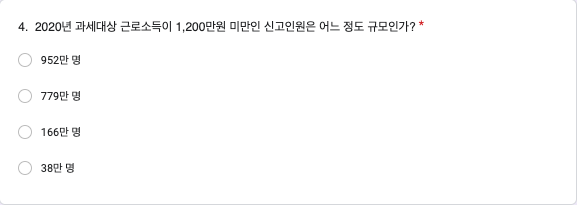
\includegraphics[width=0.75\linewidth]{./pics/Quiz230315_Q4}

\subsection{과세대상 근로소득 1,200만 원(집계표)}\label{uxacfcuxc138uxb300uxc0c1-uxadfcuxb85cuxc18cuxb4dd-1200uxb9cc-uxc6d0uxc9d1uxacc4uxd45c}

\begin{longtable}[]{@{}
  >{\raggedright\arraybackslash}p{(\linewidth - 10\tabcolsep) * \real{0.1667}}
  >{\centering\arraybackslash}p{(\linewidth - 10\tabcolsep) * \real{0.1528}}
  >{\centering\arraybackslash}p{(\linewidth - 10\tabcolsep) * \real{0.1528}}
  >{\centering\arraybackslash}p{(\linewidth - 10\tabcolsep) * \real{0.1528}}
  >{\centering\arraybackslash}p{(\linewidth - 10\tabcolsep) * \real{0.1389}}
  >{\centering\arraybackslash}p{(\linewidth - 10\tabcolsep) * \real{0.0833}}@{}}
\toprule\noalign{}
\begin{minipage}[b]{\linewidth}\raggedright
~
\end{minipage} & \begin{minipage}[b]{\linewidth}\centering
952만 명
\end{minipage} & \begin{minipage}[b]{\linewidth}\centering
779만 명
\end{minipage} & \begin{minipage}[b]{\linewidth}\centering
166만 명
\end{minipage} & \begin{minipage}[b]{\linewidth}\centering
38만 명
\end{minipage} & \begin{minipage}[b]{\linewidth}\centering
계
\end{minipage} \\
\midrule\noalign{}
\endhead
\bottomrule\noalign{}
\endlastfoot
\textbf{Red} & 158 & 71 & 39 & 9 & 277 \\
\textbf{Black} & 150 & 74 & 47 & 5 & 276 \\
\textbf{계} & 308 & 145 & 86 & 14 & 553 \\
\end{longtable}

\begin{longtable}[]{@{}
  >{\raggedleft\arraybackslash}p{(\linewidth - 4\tabcolsep) * \real{0.2361}}
  >{\raggedleft\arraybackslash}p{(\linewidth - 4\tabcolsep) * \real{0.0694}}
  >{\raggedleft\arraybackslash}p{(\linewidth - 4\tabcolsep) * \real{0.1389}}@{}}
\caption{Pearson's Chi-squared test: \texttt{.}}\tabularnewline
\toprule\noalign{}
\begin{minipage}[b]{\linewidth}\raggedleft
Test statistic
\end{minipage} & \begin{minipage}[b]{\linewidth}\raggedleft
df
\end{minipage} & \begin{minipage}[b]{\linewidth}\raggedleft
P value
\end{minipage} \\
\midrule\noalign{}
\endfirsthead
\toprule\noalign{}
\begin{minipage}[b]{\linewidth}\raggedleft
Test statistic
\end{minipage} & \begin{minipage}[b]{\linewidth}\raggedleft
df
\end{minipage} & \begin{minipage}[b]{\linewidth}\raggedleft
P value
\end{minipage} \\
\midrule\noalign{}
\endhead
\bottomrule\noalign{}
\endlastfoot
2.155 & 3 & 0.5408 \\
\end{longtable}

Q4의 집계 결과가 Red, Black 간에 통계적으로 유의한 차이가 있는지 알아보기 위하여 카이제곱 테스트를 수행하였습니다.

그 결과 카이제곱 통계량은 2.155, 자유도는 3, p-value 는 0.5408이므로 Red, Black 간에 통계적으로 유의한 차이를 보이지 않습니다.

실제로 닮은 게 느껴집니까?

\subsection{과세대상 근로소득 1,200만 원(\%)}\label{uxacfcuxc138uxb300uxc0c1-uxadfcuxb85cuxc18cuxb4dd-1200uxb9cc-uxc6d0}

\begin{longtable}[]{@{}
  >{\centering\arraybackslash}p{(\linewidth - 8\tabcolsep) * \real{0.1528}}
  >{\centering\arraybackslash}p{(\linewidth - 8\tabcolsep) * \real{0.1528}}
  >{\centering\arraybackslash}p{(\linewidth - 8\tabcolsep) * \real{0.1528}}
  >{\centering\arraybackslash}p{(\linewidth - 8\tabcolsep) * \real{0.1389}}
  >{\centering\arraybackslash}p{(\linewidth - 8\tabcolsep) * \real{0.1389}}@{}}
\toprule\noalign{}
\begin{minipage}[b]{\linewidth}\centering
952만 명
\end{minipage} & \begin{minipage}[b]{\linewidth}\centering
779만 명
\end{minipage} & \begin{minipage}[b]{\linewidth}\centering
166만 명
\end{minipage} & \begin{minipage}[b]{\linewidth}\centering
38만 명
\end{minipage} & \begin{minipage}[b]{\linewidth}\centering
계
\end{minipage} \\
\midrule\noalign{}
\endhead
\bottomrule\noalign{}
\endlastfoot
55.7 & 26.2 & 15.6 & 2.5 & 100.0 \\
\end{longtable}

정답률은 Red, Black 을 합하여 계산하는데, 55.7(\%) 입니다.

\section{Q5. 소득세 실효세율}\label{q5.-uxc18cuxb4dduxc138-uxc2e4uxd6a8uxc138uxc728}


\includegraphics[width=0.75\linewidth]{./pics/Quiz230315_Q5}

\subsection{소득세 실효세율(집계표)}\label{uxc18cuxb4dduxc138-uxc2e4uxd6a8uxc138uxc728uxc9d1uxacc4uxd45c}

\begin{longtable}[]{@{}
  >{\raggedright\arraybackslash}p{(\linewidth - 10\tabcolsep) * \real{0.1667}}
  >{\raggedleft\arraybackslash}p{(\linewidth - 10\tabcolsep) * \real{0.0972}}
  >{\raggedleft\arraybackslash}p{(\linewidth - 10\tabcolsep) * \real{0.1111}}
  >{\raggedleft\arraybackslash}p{(\linewidth - 10\tabcolsep) * \real{0.1111}}
  >{\raggedleft\arraybackslash}p{(\linewidth - 10\tabcolsep) * \real{0.0972}}
  >{\centering\arraybackslash}p{(\linewidth - 10\tabcolsep) * \real{0.0972}}@{}}
\toprule\noalign{}
\begin{minipage}[b]{\linewidth}\raggedright
~
\end{minipage} & \begin{minipage}[b]{\linewidth}\raggedleft
0.2\%
\end{minipage} & \begin{minipage}[b]{\linewidth}\raggedleft
15.1\%
\end{minipage} & \begin{minipage}[b]{\linewidth}\raggedleft
37.4\%
\end{minipage} & \begin{minipage}[b]{\linewidth}\raggedleft
5.9\%
\end{minipage} & \begin{minipage}[b]{\linewidth}\centering
계
\end{minipage} \\
\midrule\noalign{}
\endhead
\bottomrule\noalign{}
\endlastfoot
\textbf{Red} & 2 & 58 & 19 & 198 & 277 \\
\textbf{Black} & 8 & 48 & 16 & 204 & 276 \\
\textbf{계} & 10 & 106 & 35 & 402 & 553 \\
\end{longtable}

\begin{longtable}[]{@{}
  >{\raggedleft\arraybackslash}p{(\linewidth - 4\tabcolsep) * \real{0.2361}}
  >{\raggedleft\arraybackslash}p{(\linewidth - 4\tabcolsep) * \real{0.0694}}
  >{\raggedleft\arraybackslash}p{(\linewidth - 4\tabcolsep) * \real{0.1389}}@{}}
\caption{Pearson's Chi-squared test: \texttt{.}}\tabularnewline
\toprule\noalign{}
\begin{minipage}[b]{\linewidth}\raggedleft
Test statistic
\end{minipage} & \begin{minipage}[b]{\linewidth}\raggedleft
df
\end{minipage} & \begin{minipage}[b]{\linewidth}\raggedleft
P value
\end{minipage} \\
\midrule\noalign{}
\endfirsthead
\toprule\noalign{}
\begin{minipage}[b]{\linewidth}\raggedleft
Test statistic
\end{minipage} & \begin{minipage}[b]{\linewidth}\raggedleft
df
\end{minipage} & \begin{minipage}[b]{\linewidth}\raggedleft
P value
\end{minipage} \\
\midrule\noalign{}
\endhead
\bottomrule\noalign{}
\endlastfoot
4.888 & 3 & 0.1802 \\
\end{longtable}

Q5의 집계 결과가 Red, Black 간에 통계적으로 유의한 차이가 있는지 알아보기 위하여 카이제곱 테스트를 수행하였습니다.

그 결과 카이제곱 통계량은 4.888, 자유도는 3, p-value 는 0.1802이므로 Red, Black 간에 통계적으로 유의한 차이를 보이지 않습니다.

실제로 닮은 게 느껴집니까?

\subsection{소득세 실효세율(\%)}\label{uxc18cuxb4dduxc138-uxc2e4uxd6a8uxc138uxc728}

\begin{longtable}[]{@{}
  >{\raggedleft\arraybackslash}p{(\linewidth - 8\tabcolsep) * \real{0.0972}}
  >{\raggedleft\arraybackslash}p{(\linewidth - 8\tabcolsep) * \real{0.1111}}
  >{\raggedleft\arraybackslash}p{(\linewidth - 8\tabcolsep) * \real{0.1111}}
  >{\raggedleft\arraybackslash}p{(\linewidth - 8\tabcolsep) * \real{0.0972}}
  >{\centering\arraybackslash}p{(\linewidth - 8\tabcolsep) * \real{0.1111}}@{}}
\toprule\noalign{}
\begin{minipage}[b]{\linewidth}\raggedleft
0.2\%
\end{minipage} & \begin{minipage}[b]{\linewidth}\raggedleft
15.1\%
\end{minipage} & \begin{minipage}[b]{\linewidth}\raggedleft
37.4\%
\end{minipage} & \begin{minipage}[b]{\linewidth}\raggedleft
5.9\%
\end{minipage} & \begin{minipage}[b]{\linewidth}\centering
계
\end{minipage} \\
\midrule\noalign{}
\endhead
\bottomrule\noalign{}
\endlastfoot
1.8 & 19.2 & 6.3 & 72.7 & 100.0 \\
\end{longtable}

정답률은 Red, Black 을 합하여 계산하는데, 72.7(\%) 입니다.

\section{Q6. 기업규모별 과세 현황}\label{q6.-uxae30uxc5c5uxaddcuxbaa8uxbcc4-uxacfcuxc138-uxd604uxd669}

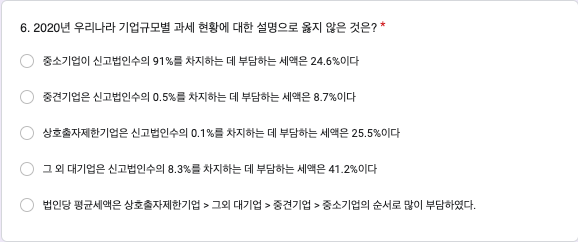
\includegraphics[width=0.75\linewidth]{./pics/Quiz230315_Q6}

\subsection{기업규모별 과세 현황(집계표)}\label{uxae30uxc5c5uxaddcuxbaa8uxbcc4-uxacfcuxc138-uxd604uxd669uxc9d1uxacc4uxd45c}

\begin{longtable}[]{@{}
  >{\raggedright\arraybackslash}p{(\linewidth - 12\tabcolsep) * \real{0.0678}}
  >{\centering\arraybackslash}p{(\linewidth - 12\tabcolsep) * \real{0.1808}}
  >{\centering\arraybackslash}p{(\linewidth - 12\tabcolsep) * \real{0.1864}}
  >{\centering\arraybackslash}p{(\linewidth - 12\tabcolsep) * \real{0.1751}}
  >{\centering\arraybackslash}p{(\linewidth - 12\tabcolsep) * \real{0.1695}}
  >{\centering\arraybackslash}p{(\linewidth - 12\tabcolsep) * \real{0.1864}}
  >{\centering\arraybackslash}p{(\linewidth - 12\tabcolsep) * \real{0.0339}}@{}}
\toprule\noalign{}
\begin{minipage}[b]{\linewidth}\raggedright
~
\end{minipage} & \begin{minipage}[b]{\linewidth}\centering
중소기업이 신고법인수의 91\%를
차지하는 데 부담하는 세액은
24.6\%이다
\end{minipage} & \begin{minipage}[b]{\linewidth}\centering
중견기업은 신고법인수의 0.5\%를
차지하는 데 부담하는 세액은
8.7\%이다
\end{minipage} & \begin{minipage}[b]{\linewidth}\centering
상호출자제한기업은
신고법인수의 0.1\%를 차지하는
데 부담하는 세액은 25.5\%이다
\end{minipage} & \begin{minipage}[b]{\linewidth}\centering
그 외 대기업은 신고법인수의
8.3\%를 차지하는 데 부담하는
세액은 41.2\%이다
\end{minipage} & \begin{minipage}[b]{\linewidth}\centering
법인당 평균세액은
상호출자제한기업 \textgreater{} 그외 대기업
\textgreater{} 중견기업 \textgreater{} 중소기업의 순서로
많이 부담하였다.
\end{minipage} & \begin{minipage}[b]{\linewidth}\centering
계
\end{minipage} \\
\midrule\noalign{}
\endhead
\bottomrule\noalign{}
\endlastfoot
\textbf{Red} & 14 & 37 & 38 & 50 & 138 & 277 \\
\textbf{Black} & 18 & 33 & 21 & 61 & 143 & 276 \\
\textbf{계} & 32 & 70 & 59 & 111 & 281 & 553 \\
\end{longtable}

\begin{longtable}[]{@{}
  >{\raggedleft\arraybackslash}p{(\linewidth - 4\tabcolsep) * \real{0.2361}}
  >{\raggedleft\arraybackslash}p{(\linewidth - 4\tabcolsep) * \real{0.0694}}
  >{\raggedleft\arraybackslash}p{(\linewidth - 4\tabcolsep) * \real{0.1389}}@{}}
\caption{Pearson's Chi-squared test: \texttt{.}}\tabularnewline
\toprule\noalign{}
\begin{minipage}[b]{\linewidth}\raggedleft
Test statistic
\end{minipage} & \begin{minipage}[b]{\linewidth}\raggedleft
df
\end{minipage} & \begin{minipage}[b]{\linewidth}\raggedleft
P value
\end{minipage} \\
\midrule\noalign{}
\endfirsthead
\toprule\noalign{}
\begin{minipage}[b]{\linewidth}\raggedleft
Test statistic
\end{minipage} & \begin{minipage}[b]{\linewidth}\raggedleft
df
\end{minipage} & \begin{minipage}[b]{\linewidth}\raggedleft
P value
\end{minipage} \\
\midrule\noalign{}
\endhead
\bottomrule\noalign{}
\endlastfoot
6.804 & 4 & 0.1466 \\
\end{longtable}

Q6의 집계 결과가 Red, Black 간에 통계적으로 유의한 차이가 있는지 알아보기 위하여 카이제곱 테스트를 수행하였습니다.

그 결과 카이제곱 통계량은 6.804, 자유도는 4, p-value 는 0.1466이므로 Red, Black 간에 통계적으로 유의한 차이를 보이지 않습니다.

실제로 닮은 게 느껴집니까?

\subsection{기업규모별 과세 현황(\%)}\label{uxae30uxc5c5uxaddcuxbaa8uxbcc4-uxacfcuxc138-uxd604uxd669}

\begin{longtable}[]{@{}
  >{\centering\arraybackslash}p{(\linewidth - 10\tabcolsep) * \real{0.1916}}
  >{\centering\arraybackslash}p{(\linewidth - 10\tabcolsep) * \real{0.1976}}
  >{\centering\arraybackslash}p{(\linewidth - 10\tabcolsep) * \real{0.1856}}
  >{\centering\arraybackslash}p{(\linewidth - 10\tabcolsep) * \real{0.1796}}
  >{\centering\arraybackslash}p{(\linewidth - 10\tabcolsep) * \real{0.1976}}
  >{\centering\arraybackslash}p{(\linewidth - 10\tabcolsep) * \real{0.0479}}@{}}
\toprule\noalign{}
\begin{minipage}[b]{\linewidth}\centering
중소기업이 신고법인수의 91\%를
차지하는 데 부담하는 세액은
24.6\%이다
\end{minipage} & \begin{minipage}[b]{\linewidth}\centering
중견기업은 신고법인수의 0.5\%를
차지하는 데 부담하는 세액은
8.7\%이다
\end{minipage} & \begin{minipage}[b]{\linewidth}\centering
상호출자제한기업은
신고법인수의 0.1\%를 차지하는
데 부담하는 세액은 25.5\%이다
\end{minipage} & \begin{minipage}[b]{\linewidth}\centering
그 외 대기업은 신고법인수의
8.3\%를 차지하는 데 부담하는
세액은 41.2\%이다
\end{minipage} & \begin{minipage}[b]{\linewidth}\centering
법인당 평균세액은
상호출자제한기업 \textgreater{} 그외 대기업
\textgreater{} 중견기업 \textgreater{} 중소기업의 순서로
많이 부담하였다.
\end{minipage} & \begin{minipage}[b]{\linewidth}\centering
계
\end{minipage} \\
\midrule\noalign{}
\endhead
\bottomrule\noalign{}
\endlastfoot
5.8 & 12.7 & 10.7 & 20.1 & 50.8 & 100.0 \\
\end{longtable}

정답률은 Red, Black 을 합하여 계산하는데, 50.8(\%) 입니다.

\section{Q7. 국민부담률 적정 수준 : 아일랜드와 OECD 평균}\label{q7.-uxad6duxbbfcuxbd80uxb2f4uxb960-uxc801uxc815-uxc218uxc900-uxc544uxc77cuxb79cuxb4dcuxc640-oecd-uxd3c9uxade0}

질문 내용에 의도하는 바를 담으면 어떨까요?

OECD 국가 중 국민부담률이 매우 낮은 편인 아일랜드의 사례를 들어서 감세정책이 가져온 긍정적인 효과에 대해서 설명하고 우리나라의 바람직한 조정 방향은 무엇이냐고 묻는 것을 Red, 감세 정책이 가져온 부정적인 효과에 대해서 설명하고 우리나라의 바람직한 조정 방향은 무엇이냐고 묻는 것을 Black 에 배치했을 때, 설명이 응답에 영향을 미치지 않으면 Red 와 Black에 차이가 없어야 할텐데 집계결과는 어떻게 나오고 있나요?

분명히 영향을 미치고 있는 것으로 보입니다.

통계적으로 매우 유의한 차이가 관찰되고 있습니다.

감세정책의 효과가 긍정적이라고 설명한 Red 에서는 낮춰야 한다는 응답이, 감세정책의 효과가 부정적이라고 설명한 Black 에서는 높여야 한다는 응답이 높게 나온 것을 볼 수 있고, 따라서 p-value 가 엄청나게 작은 값을 보여주고 있습니다.

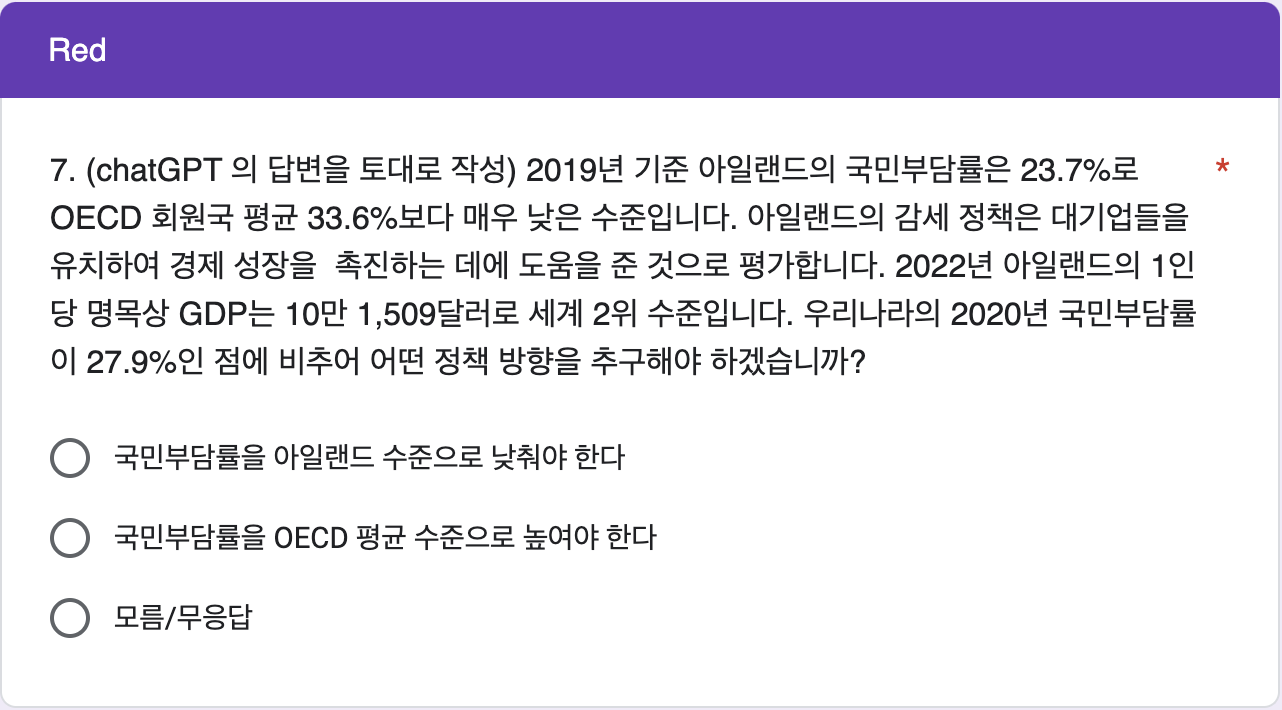
\includegraphics[width=0.67\linewidth]{./pics/Quiz240315_Q7_Red}

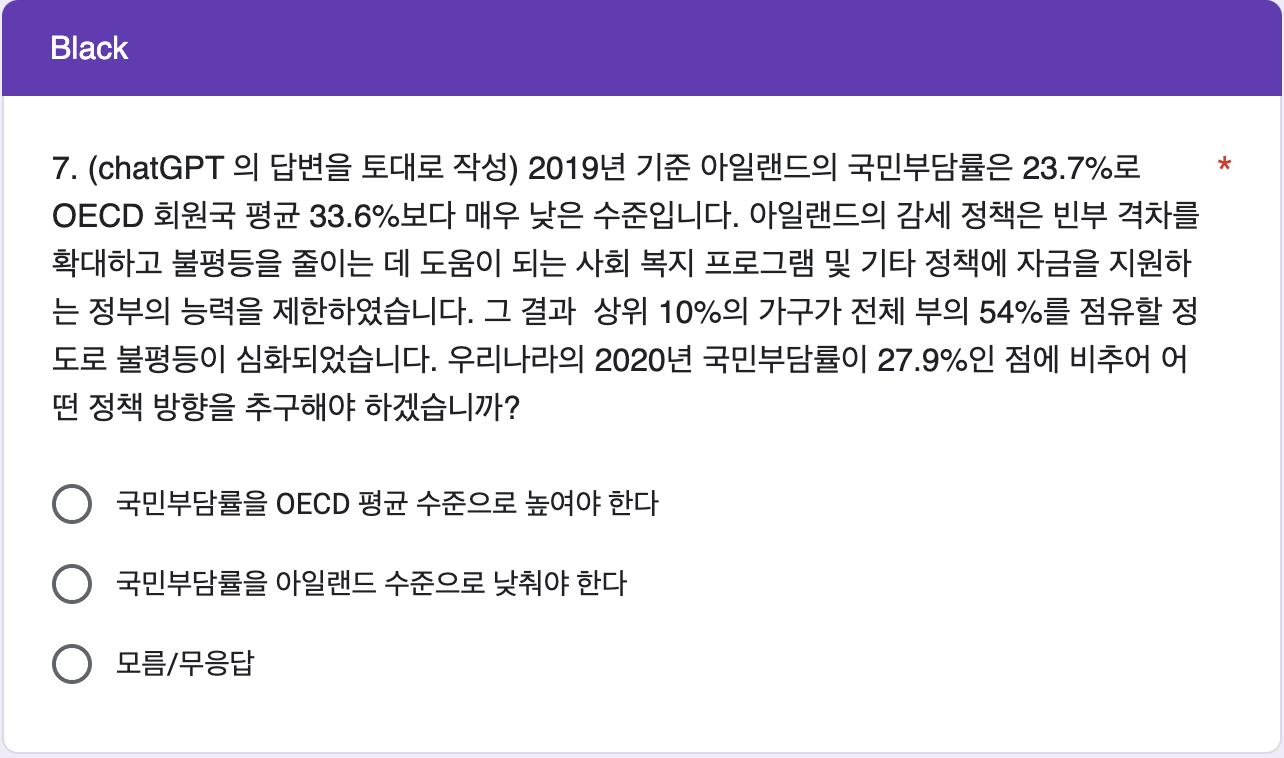
\includegraphics[width=0.67\linewidth]{./pics/Quiz240315_Q7_Black}

\subsection{집계표}\label{uxc9d1uxacc4uxd45c-1}

\begin{longtable}[]{@{}
  >{\raggedright\arraybackslash}p{(\linewidth - 8\tabcolsep) * \real{0.3766}}
  >{\centering\arraybackslash}p{(\linewidth - 8\tabcolsep) * \real{0.1818}}
  >{\centering\arraybackslash}p{(\linewidth - 8\tabcolsep) * \real{0.1818}}
  >{\centering\arraybackslash}p{(\linewidth - 8\tabcolsep) * \real{0.1818}}
  >{\centering\arraybackslash}p{(\linewidth - 8\tabcolsep) * \real{0.0779}}@{}}
\toprule\noalign{}
\begin{minipage}[b]{\linewidth}\raggedright
~
\end{minipage} & \begin{minipage}[b]{\linewidth}\centering
낮춰야 한다
\end{minipage} & \begin{minipage}[b]{\linewidth}\centering
높여야 한다
\end{minipage} & \begin{minipage}[b]{\linewidth}\centering
모름/무응답
\end{minipage} & \begin{minipage}[b]{\linewidth}\centering
계
\end{minipage} \\
\midrule\noalign{}
\endhead
\bottomrule\noalign{}
\endlastfoot
\textbf{Red(감세의 긍정적효과
설명)} & 90 & 120 & 67 & 277 \\
\textbf{Black(감세의 부정적 효과
설명)} & 46 & 168 & 62 & 276 \\
\textbf{계} & 136 & 288 & 129 & 553 \\
\end{longtable}

\begin{longtable}[]{@{}
  >{\raggedleft\arraybackslash}p{(\linewidth - 4\tabcolsep) * \real{0.2361}}
  >{\raggedleft\arraybackslash}p{(\linewidth - 4\tabcolsep) * \real{0.0694}}
  >{\raggedleft\arraybackslash}p{(\linewidth - 4\tabcolsep) * \real{0.2500}}@{}}
\caption{Pearson's Chi-squared test: \texttt{.}}\tabularnewline
\toprule\noalign{}
\begin{minipage}[b]{\linewidth}\raggedleft
Test statistic
\end{minipage} & \begin{minipage}[b]{\linewidth}\raggedleft
df
\end{minipage} & \begin{minipage}[b]{\linewidth}\raggedleft
P value
\end{minipage} \\
\midrule\noalign{}
\endfirsthead
\toprule\noalign{}
\begin{minipage}[b]{\linewidth}\raggedleft
Test statistic
\end{minipage} & \begin{minipage}[b]{\linewidth}\raggedleft
df
\end{minipage} & \begin{minipage}[b]{\linewidth}\raggedleft
P value
\end{minipage} \\
\midrule\noalign{}
\endhead
\bottomrule\noalign{}
\endlastfoot
22.43 & 2 & 1.349e-05 * * * \\
\end{longtable}

Q7의 Red에는 아일랜드의 사례에서 감세 정책의 긍정적 측면을 설명한 후 우리나라 조세 정책의 방향에 대하여 물었을 때, 277명이 응답한 가운데 90명이 우리나라의 국민부담률을 아일랜드 수준으로 ``낮춰야 한다''는 반응을 보이고, 120명이 OECD평균 수준으로 ``높여야 한다''는 반응을 보입니다.

Black은 같은 아일랜드의 사례에서 감세 정책의 부정적 측면을 설명한 후 우리나라 조세 정책의 방향에 대하여 물었을 떄, 276명이 응답한 가운데 46명이 우리나라의 국민부담률을 아일랜드 수준으로 ``낮춰야 한다''는 반응을 보이고, 168명이 OECD 평균 수준으로 ``높여야 한다''는 반응을 보입니다.

그리고 ``모름/무응답''에 답한 인원은 Red에 67명, Black 에 62명이 응답하였습니다.

우연일까요?

모름/무응답에 있어서는 Red, Black이 몹시 닮았습니다.

카이제곱 테스트는 이와 같은 상황에서 감세정책의 긍정적 측면을 부각시킨 경우와 부정적 측면을 부각시킨 경우에 그 차이가 통계적으로 매우, 매우, \ldots{} 유의하다는 것을 보여 줍니다.

카이제곱 통계량은 22.427, 자유도는 2, p-value 는 1.3e-05으로
감세정책의 어떤 측면을 설명하느냐에 따라 반응이 다르게 나온다는 것을 보여줍니다.

여기서 질문 내용에 의도하는 바를 담더라도 응답에 영향을 끼치지 않는다고 가정합니다.

랜덤화의 효과로 Red, Black 의 응답은 닮게 마련입니다.

즉, 통계적으로 유의한 차이를 보이지 않게 됩니다.

그러나 실제로 관찰된 카이제곱 통계값의 P-value 는 0.05보다 매우 작은 값입니다.

따라서, 질문 내용에 의도하는 바를 담더라도 영향을 끼치지 않는다는 가정은 잘못된 것이죠.

이러한 논증 방식을 귀류법이라고 합니다.

\subsection{\% 비교}\label{uxbe44uxad50-1}

\begin{longtable}[]{@{}
  >{\raggedright\arraybackslash}p{(\linewidth - 8\tabcolsep) * \real{0.3671}}
  >{\centering\arraybackslash}p{(\linewidth - 8\tabcolsep) * \real{0.1772}}
  >{\centering\arraybackslash}p{(\linewidth - 8\tabcolsep) * \real{0.1772}}
  >{\centering\arraybackslash}p{(\linewidth - 8\tabcolsep) * \real{0.1772}}
  >{\centering\arraybackslash}p{(\linewidth - 8\tabcolsep) * \real{0.1013}}@{}}
\toprule\noalign{}
\begin{minipage}[b]{\linewidth}\raggedright
~
\end{minipage} & \begin{minipage}[b]{\linewidth}\centering
낮춰야 한다
\end{minipage} & \begin{minipage}[b]{\linewidth}\centering
높여야 한다
\end{minipage} & \begin{minipage}[b]{\linewidth}\centering
모름/무응답
\end{minipage} & \begin{minipage}[b]{\linewidth}\centering
계
\end{minipage} \\
\midrule\noalign{}
\endhead
\bottomrule\noalign{}
\endlastfoot
\textbf{Red(감세의 긍정적효과
설명)} & 32.5 & 43.3 & 24.2 & 100.0 \\
\textbf{Black(감세의 부정적 효과
설명)} & 16.7 & 60.9 & 22.5 & 100.0 \\
\end{longtable}

감세정책의 긍정적 측면을 설명한 Red에서 우리나라의 국민부담률을 ``낮춰야 한다''고 응답하는사람들의 백분율, 32.5(\%)은 ``높여야 한다''고 응답하는 사람들의 백분율, 43.3(\%) 보다 높습니다.

반면 감세정책의 부정적 측면을 설명한 Black에서 우리나라의 국민 부담률을 ``낮춰야 한다''고 응답하는 사람들의 백분율, 16.7(\%)은 ``높여야 한다''고 응답하는 사람들의 백분율, 60.9(\%) 보다 훨씬 적습니다.

어느 정책의 긍정적 측면을 설명하느냐, 부정적 측면을 설명하느냐에 따라 반응이 달라진다는 것을 잘 알 수 있습니다.

Red 와 Black 이 워낙 차이가 나지만 전체적으로 어느 정도가 우리나라의 국민부담률을 ``낮춰야 한다''하고 어느 정도가 ``높여야 한다''고 응답하였는지 합쳐 보겠습니다.

\subsection{\% 합계}\label{uxd569uxacc4}

\begin{longtable}[]{@{}
  >{\centering\arraybackslash}p{(\linewidth - 6\tabcolsep) * \real{0.1944}}
  >{\centering\arraybackslash}p{(\linewidth - 6\tabcolsep) * \real{0.1944}}
  >{\centering\arraybackslash}p{(\linewidth - 6\tabcolsep) * \real{0.1944}}
  >{\centering\arraybackslash}p{(\linewidth - 6\tabcolsep) * \real{0.1111}}@{}}
\toprule\noalign{}
\begin{minipage}[b]{\linewidth}\centering
낮춰야 한다
\end{minipage} & \begin{minipage}[b]{\linewidth}\centering
높여야 한다
\end{minipage} & \begin{minipage}[b]{\linewidth}\centering
모름/무응답
\end{minipage} & \begin{minipage}[b]{\linewidth}\centering
계
\end{minipage} \\
\midrule\noalign{}
\endhead
\bottomrule\noalign{}
\endlastfoot
24.6 & 52.1 & 23.3 & 100.0 \\
\end{longtable}

우리나라의 국민부담률을 ``낮춰야 한다''고 응답한 백분율은 Red, Black 합쳐서 24.6(\%)(으)로 우리나라의 국민부담률을 '높여야한다''고 응답한 백분율, 52.1(\%) 보다 상당히 적습니다.

다만, 모름/무응답이 23.3(\%)로 적지 않습니다.

\subsection{Mosaic Plot}\label{mosaic-plot-4}

\pandocbounded{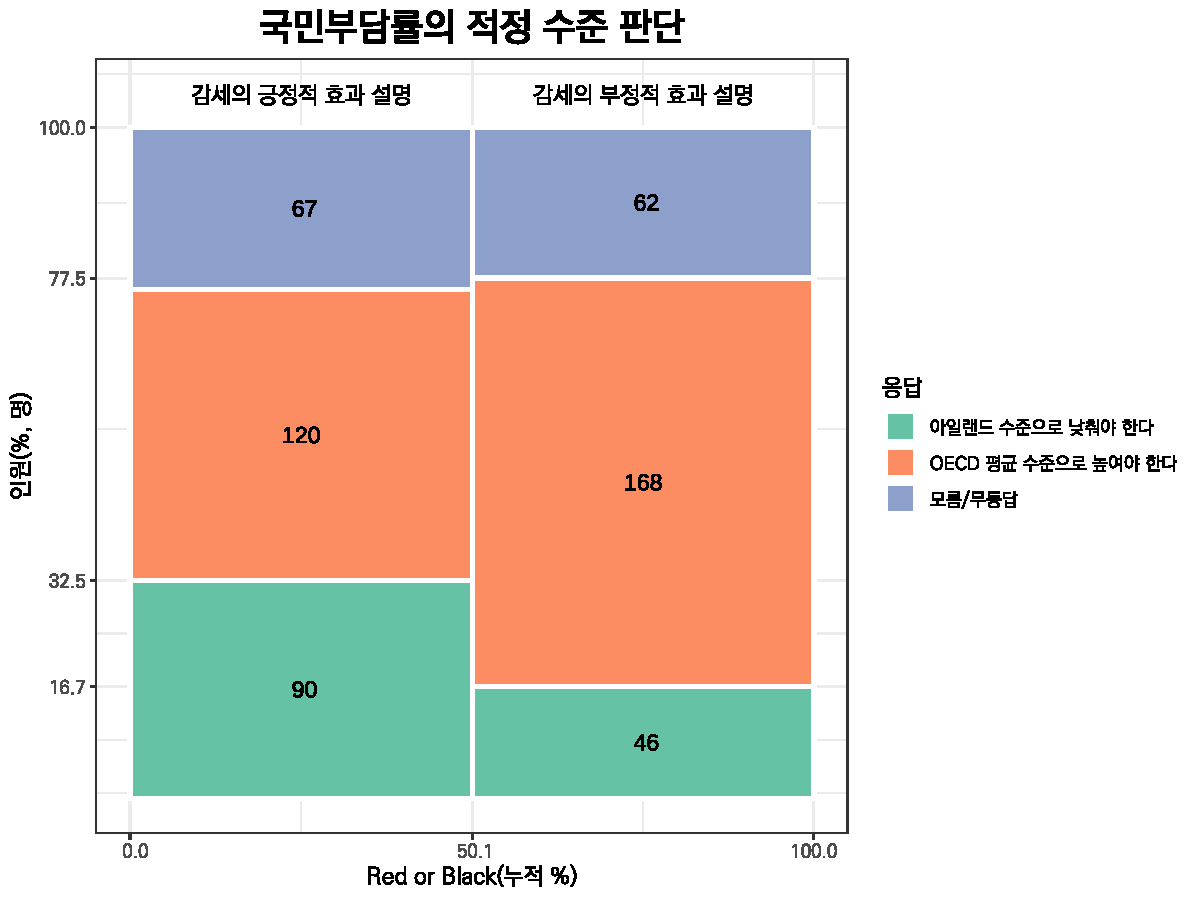
\includegraphics[keepaspectratio]{Quiz_report_2025_files/figure-latex/unnamed-chunk-60-1.pdf}}

Mosaic Plot 은 이 집계결과를 시각적으로 잘 보여줍니다.

감세정책의 긍정적 측면을 설명한 Red 에서 우리나라의 국민부담률을 ``낮춰야 한다''고 응답한 백분율이 높고, 감세정책의 부정적 측면을 설명한 Black 에서 우리나라의 국민부담률을 ``높여야 한다''고 응답한 백분율이 월등히 높은 것을 시각적으로 알 수 있습니다.

\section{마감 시간으로부터 제출 시간의 분포}\label{uxb9c8uxac10-uxc2dcuxac04uxc73cuxb85cuxbd80uxd130-uxc81cuxcd9c-uxc2dcuxac04uxc758-uxbd84uxd3ec-2}

\subsection{분포표}\label{uxbd84uxd3ecuxd45c-2}

\begin{longtable}[]{@{}
  >{\raggedright\arraybackslash}p{(\linewidth - 30\tabcolsep) * \real{0.1121}}
  >{\centering\arraybackslash}p{(\linewidth - 30\tabcolsep) * \real{0.0654}}
  >{\centering\arraybackslash}p{(\linewidth - 30\tabcolsep) * \real{0.0654}}
  >{\centering\arraybackslash}p{(\linewidth - 30\tabcolsep) * \real{0.0654}}
  >{\centering\arraybackslash}p{(\linewidth - 30\tabcolsep) * \real{0.0654}}
  >{\centering\arraybackslash}p{(\linewidth - 30\tabcolsep) * \real{0.0654}}
  >{\centering\arraybackslash}p{(\linewidth - 30\tabcolsep) * \real{0.0561}}
  >{\centering\arraybackslash}p{(\linewidth - 30\tabcolsep) * \real{0.0561}}
  >{\centering\arraybackslash}p{(\linewidth - 30\tabcolsep) * \real{0.0561}}
  >{\centering\arraybackslash}p{(\linewidth - 30\tabcolsep) * \real{0.0561}}
  >{\centering\arraybackslash}p{(\linewidth - 30\tabcolsep) * \real{0.0561}}
  >{\centering\arraybackslash}p{(\linewidth - 30\tabcolsep) * \real{0.0561}}
  >{\centering\arraybackslash}p{(\linewidth - 30\tabcolsep) * \real{0.0561}}
  >{\centering\arraybackslash}p{(\linewidth - 30\tabcolsep) * \real{0.0561}}
  >{\centering\arraybackslash}p{(\linewidth - 30\tabcolsep) * \real{0.0561}}
  >{\centering\arraybackslash}p{(\linewidth - 30\tabcolsep) * \real{0.0561}}@{}}
\caption{일 단위}\tabularnewline
\toprule\noalign{}
\begin{minipage}[b]{\linewidth}\raggedright
~
\end{minipage} & \begin{minipage}[b]{\linewidth}\centering
14일
\end{minipage} & \begin{minipage}[b]{\linewidth}\centering
13일
\end{minipage} & \begin{minipage}[b]{\linewidth}\centering
12일
\end{minipage} & \begin{minipage}[b]{\linewidth}\centering
11일
\end{minipage} & \begin{minipage}[b]{\linewidth}\centering
10일
\end{minipage} & \begin{minipage}[b]{\linewidth}\centering
9일
\end{minipage} & \begin{minipage}[b]{\linewidth}\centering
8일
\end{minipage} & \begin{minipage}[b]{\linewidth}\centering
7일
\end{minipage} & \begin{minipage}[b]{\linewidth}\centering
6일
\end{minipage} & \begin{minipage}[b]{\linewidth}\centering
5일
\end{minipage} & \begin{minipage}[b]{\linewidth}\centering
4일
\end{minipage} & \begin{minipage}[b]{\linewidth}\centering
3일
\end{minipage} & \begin{minipage}[b]{\linewidth}\centering
2일
\end{minipage} & \begin{minipage}[b]{\linewidth}\centering
1일
\end{minipage} & \begin{minipage}[b]{\linewidth}\centering
계
\end{minipage} \\
\midrule\noalign{}
\endfirsthead
\toprule\noalign{}
\begin{minipage}[b]{\linewidth}\raggedright
~
\end{minipage} & \begin{minipage}[b]{\linewidth}\centering
14일
\end{minipage} & \begin{minipage}[b]{\linewidth}\centering
13일
\end{minipage} & \begin{minipage}[b]{\linewidth}\centering
12일
\end{minipage} & \begin{minipage}[b]{\linewidth}\centering
11일
\end{minipage} & \begin{minipage}[b]{\linewidth}\centering
10일
\end{minipage} & \begin{minipage}[b]{\linewidth}\centering
9일
\end{minipage} & \begin{minipage}[b]{\linewidth}\centering
8일
\end{minipage} & \begin{minipage}[b]{\linewidth}\centering
7일
\end{minipage} & \begin{minipage}[b]{\linewidth}\centering
6일
\end{minipage} & \begin{minipage}[b]{\linewidth}\centering
5일
\end{minipage} & \begin{minipage}[b]{\linewidth}\centering
4일
\end{minipage} & \begin{minipage}[b]{\linewidth}\centering
3일
\end{minipage} & \begin{minipage}[b]{\linewidth}\centering
2일
\end{minipage} & \begin{minipage}[b]{\linewidth}\centering
1일
\end{minipage} & \begin{minipage}[b]{\linewidth}\centering
계
\end{minipage} \\
\midrule\noalign{}
\endhead
\bottomrule\noalign{}
\endlastfoot
\textbf{Red} & 71 & 12 & 6 & 8 & 4 & 6 & 16 & 48 & 20 & 14 & 18 & 17 & 16 & 21 & 277 \\
\textbf{Black} & 64 & 14 & 3 & 6 & 10 & 4 & 4 & 47 & 30 & 18 & 12 & 17 & 22 & 25 & 276 \\
\textbf{계} & 135 & 26 & 9 & 14 & 14 & 10 & 20 & 95 & 50 & 32 & 30 & 34 & 38 & 46 & 553 \\
\end{longtable}

분포표로부터 두 가지 문제를 살펴보겠습니다.

첫째, 날마다 고르게 제출하는가?

둘째, Red, Black 간에 통계적으로 유의한 차이가 있는가?

각 문제를 살펴보기 위해서는 분포표의 일부분을 대상으로 카이제곱 테스트를 수행합니다.

\subsection{날마다 고르게 제출하는가?}\label{uxb0a0uxb9c8uxb2e4-uxace0uxb974uxac8c-uxc81cuxcd9cuxd558uxb294uxac00-2}

\begin{longtable}[]{@{}
  >{\centering\arraybackslash}p{(\linewidth - 26\tabcolsep) * \real{0.0787}}
  >{\centering\arraybackslash}p{(\linewidth - 26\tabcolsep) * \real{0.0787}}
  >{\centering\arraybackslash}p{(\linewidth - 26\tabcolsep) * \real{0.0787}}
  >{\centering\arraybackslash}p{(\linewidth - 26\tabcolsep) * \real{0.0787}}
  >{\centering\arraybackslash}p{(\linewidth - 26\tabcolsep) * \real{0.0787}}
  >{\centering\arraybackslash}p{(\linewidth - 26\tabcolsep) * \real{0.0674}}
  >{\centering\arraybackslash}p{(\linewidth - 26\tabcolsep) * \real{0.0674}}
  >{\centering\arraybackslash}p{(\linewidth - 26\tabcolsep) * \real{0.0674}}
  >{\centering\arraybackslash}p{(\linewidth - 26\tabcolsep) * \real{0.0674}}
  >{\centering\arraybackslash}p{(\linewidth - 26\tabcolsep) * \real{0.0674}}
  >{\centering\arraybackslash}p{(\linewidth - 26\tabcolsep) * \real{0.0674}}
  >{\centering\arraybackslash}p{(\linewidth - 26\tabcolsep) * \real{0.0674}}
  >{\centering\arraybackslash}p{(\linewidth - 26\tabcolsep) * \real{0.0674}}
  >{\centering\arraybackslash}p{(\linewidth - 26\tabcolsep) * \real{0.0674}}@{}}
\toprule\noalign{}
\begin{minipage}[b]{\linewidth}\centering
14일
\end{minipage} & \begin{minipage}[b]{\linewidth}\centering
13일
\end{minipage} & \begin{minipage}[b]{\linewidth}\centering
12일
\end{minipage} & \begin{minipage}[b]{\linewidth}\centering
11일
\end{minipage} & \begin{minipage}[b]{\linewidth}\centering
10일
\end{minipage} & \begin{minipage}[b]{\linewidth}\centering
9일
\end{minipage} & \begin{minipage}[b]{\linewidth}\centering
8일
\end{minipage} & \begin{minipage}[b]{\linewidth}\centering
7일
\end{minipage} & \begin{minipage}[b]{\linewidth}\centering
6일
\end{minipage} & \begin{minipage}[b]{\linewidth}\centering
5일
\end{minipage} & \begin{minipage}[b]{\linewidth}\centering
4일
\end{minipage} & \begin{minipage}[b]{\linewidth}\centering
3일
\end{minipage} & \begin{minipage}[b]{\linewidth}\centering
2일
\end{minipage} & \begin{minipage}[b]{\linewidth}\centering
1일
\end{minipage} \\
\midrule\noalign{}
\endhead
\bottomrule\noalign{}
\endlastfoot
135 & 26 & 9 & 14 & 14 & 10 & 20 & 95 & 50 & 32 & 30 & 34 & 38 & 46 \\
\end{longtable}

\begin{longtable}[]{@{}
  >{\raggedleft\arraybackslash}p{(\linewidth - 4\tabcolsep) * \real{0.2361}}
  >{\raggedleft\arraybackslash}p{(\linewidth - 4\tabcolsep) * \real{0.0694}}
  >{\raggedleft\arraybackslash}p{(\linewidth - 4\tabcolsep) * \real{0.2500}}@{}}
\caption{Chi-squared test for given probabilities: \texttt{.}}\tabularnewline
\toprule\noalign{}
\begin{minipage}[b]{\linewidth}\raggedleft
Test statistic
\end{minipage} & \begin{minipage}[b]{\linewidth}\raggedleft
df
\end{minipage} & \begin{minipage}[b]{\linewidth}\raggedleft
P value
\end{minipage} \\
\midrule\noalign{}
\endfirsthead
\toprule\noalign{}
\begin{minipage}[b]{\linewidth}\raggedleft
Test statistic
\end{minipage} & \begin{minipage}[b]{\linewidth}\raggedleft
df
\end{minipage} & \begin{minipage}[b]{\linewidth}\raggedleft
P value
\end{minipage} \\
\midrule\noalign{}
\endhead
\bottomrule\noalign{}
\endlastfoot
410 & 13 & 1.714e-79 * * * \\
\end{longtable}

날마다 고르게 제출하는지 알아 보았습니다.

분포표의 ``계''행에서 '계'열을 제외하고 카이제곱테스트를 수행합니다.

분포표 만으로도 쉽게 파악할 수 있지만 카이제곱테스트가 명확히 해 줍니다.

카이제곱 통계량은 410.01, 자유도는 13.00, p-value 는 1.7e-79 이므로 결코 고르게 제출한다고 말할 수 없겠습니다.

막대그래프로 살펴 보겠습니다.

\subsection{막대그래프}\label{uxb9c9uxb300uxadf8uxb798uxd504-2}

\pandocbounded{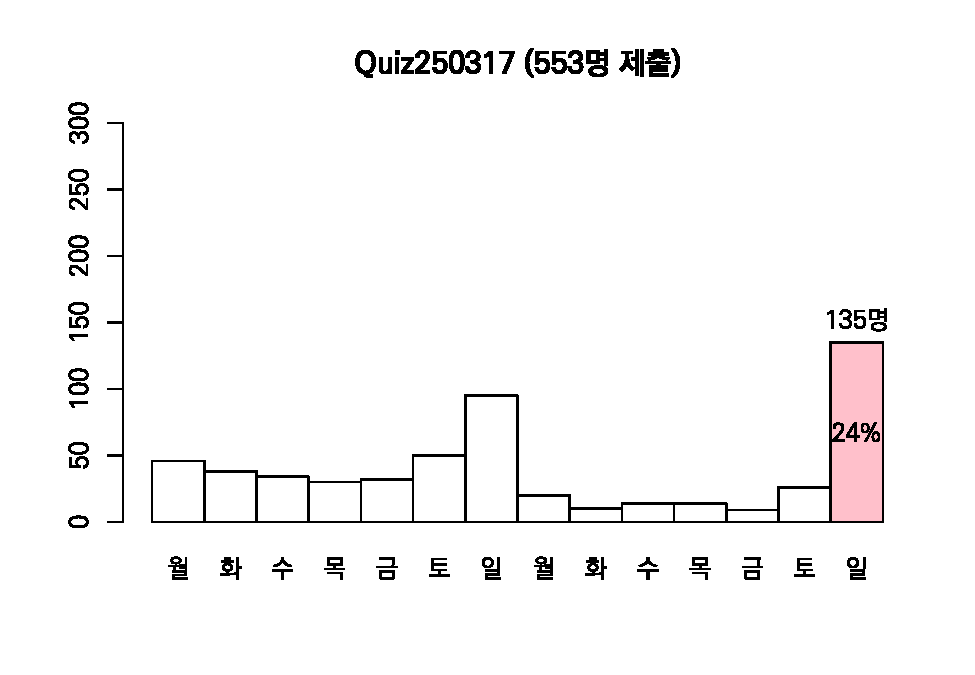
\includegraphics[keepaspectratio]{Quiz_report_2025_files/figure-latex/unnamed-chunk-63-1.pdf}}

막대그래프는 총 제출인원 553(명) 중에 135(명), 24(\%)가 마감일에 몰리는 것을 명확히 보여주고 있습니다.

\subsection{Red, Black 간에 닮았는가?}\label{red-black-uxac04uxc5d0-uxb2eeuxc558uxb294uxac00-2}

\begin{longtable}[]{@{}
  >{\raggedright\arraybackslash}p{(\linewidth - 28\tabcolsep) * \real{0.1188}}
  >{\centering\arraybackslash}p{(\linewidth - 28\tabcolsep) * \real{0.0693}}
  >{\centering\arraybackslash}p{(\linewidth - 28\tabcolsep) * \real{0.0693}}
  >{\centering\arraybackslash}p{(\linewidth - 28\tabcolsep) * \real{0.0693}}
  >{\centering\arraybackslash}p{(\linewidth - 28\tabcolsep) * \real{0.0693}}
  >{\centering\arraybackslash}p{(\linewidth - 28\tabcolsep) * \real{0.0693}}
  >{\centering\arraybackslash}p{(\linewidth - 28\tabcolsep) * \real{0.0594}}
  >{\centering\arraybackslash}p{(\linewidth - 28\tabcolsep) * \real{0.0594}}
  >{\centering\arraybackslash}p{(\linewidth - 28\tabcolsep) * \real{0.0594}}
  >{\centering\arraybackslash}p{(\linewidth - 28\tabcolsep) * \real{0.0594}}
  >{\centering\arraybackslash}p{(\linewidth - 28\tabcolsep) * \real{0.0594}}
  >{\centering\arraybackslash}p{(\linewidth - 28\tabcolsep) * \real{0.0594}}
  >{\centering\arraybackslash}p{(\linewidth - 28\tabcolsep) * \real{0.0594}}
  >{\centering\arraybackslash}p{(\linewidth - 28\tabcolsep) * \real{0.0594}}
  >{\centering\arraybackslash}p{(\linewidth - 28\tabcolsep) * \real{0.0594}}@{}}
\toprule\noalign{}
\begin{minipage}[b]{\linewidth}\raggedright
~
\end{minipage} & \begin{minipage}[b]{\linewidth}\centering
14일
\end{minipage} & \begin{minipage}[b]{\linewidth}\centering
13일
\end{minipage} & \begin{minipage}[b]{\linewidth}\centering
12일
\end{minipage} & \begin{minipage}[b]{\linewidth}\centering
11일
\end{minipage} & \begin{minipage}[b]{\linewidth}\centering
10일
\end{minipage} & \begin{minipage}[b]{\linewidth}\centering
9일
\end{minipage} & \begin{minipage}[b]{\linewidth}\centering
8일
\end{minipage} & \begin{minipage}[b]{\linewidth}\centering
7일
\end{minipage} & \begin{minipage}[b]{\linewidth}\centering
6일
\end{minipage} & \begin{minipage}[b]{\linewidth}\centering
5일
\end{minipage} & \begin{minipage}[b]{\linewidth}\centering
4일
\end{minipage} & \begin{minipage}[b]{\linewidth}\centering
3일
\end{minipage} & \begin{minipage}[b]{\linewidth}\centering
2일
\end{minipage} & \begin{minipage}[b]{\linewidth}\centering
1일
\end{minipage} \\
\midrule\noalign{}
\endhead
\bottomrule\noalign{}
\endlastfoot
\textbf{Red} & 71 & 12 & 6 & 8 & 4 & 6 & 16 & 48 & 20 & 14 & 18 & 17 & 16 & 21 \\
\textbf{Black} & 64 & 14 & 3 & 6 & 10 & 4 & 4 & 47 & 30 & 18 & 12 & 17 & 22 & 25 \\
\end{longtable}

\begin{longtable}[]{@{}
  >{\raggedleft\arraybackslash}p{(\linewidth - 4\tabcolsep) * \real{0.2361}}
  >{\raggedleft\arraybackslash}p{(\linewidth - 4\tabcolsep) * \real{0.0694}}
  >{\raggedleft\arraybackslash}p{(\linewidth - 4\tabcolsep) * \real{0.1389}}@{}}
\caption{Pearson's Chi-squared test: \texttt{.}}\tabularnewline
\toprule\noalign{}
\begin{minipage}[b]{\linewidth}\raggedleft
Test statistic
\end{minipage} & \begin{minipage}[b]{\linewidth}\raggedleft
df
\end{minipage} & \begin{minipage}[b]{\linewidth}\raggedleft
P value
\end{minipage} \\
\midrule\noalign{}
\endfirsthead
\toprule\noalign{}
\begin{minipage}[b]{\linewidth}\raggedleft
Test statistic
\end{minipage} & \begin{minipage}[b]{\linewidth}\raggedleft
df
\end{minipage} & \begin{minipage}[b]{\linewidth}\raggedleft
P value
\end{minipage} \\
\midrule\noalign{}
\endhead
\bottomrule\noalign{}
\endlastfoot
16.98 & 13 & 0.2003 \\
\end{longtable}

제출시간의 분포가 Red, Black 간에 닮았는지 알아 보았습니다.

이번에는 분포표의 첫번째와 두번째 행, '계'열을 제외한 나머지 열에 대해서 카이제곱테스트를 수행합니다.
카이제곱 통계량은 16.978, 자유도는 13, p-value 는 0.2003 이므로 제출 시간의 분포는 Red, Black 간에 통계적으로 유의한 차이가 관찰되지 않습니다.

이 사실을 Mosaic Plot을 이용하여 시각적으로 살펴보겠습니다.

닮았다고 느껴지나요?

\subsection{Mosaic Plot}\label{mosaic-plot-5}

\pandocbounded{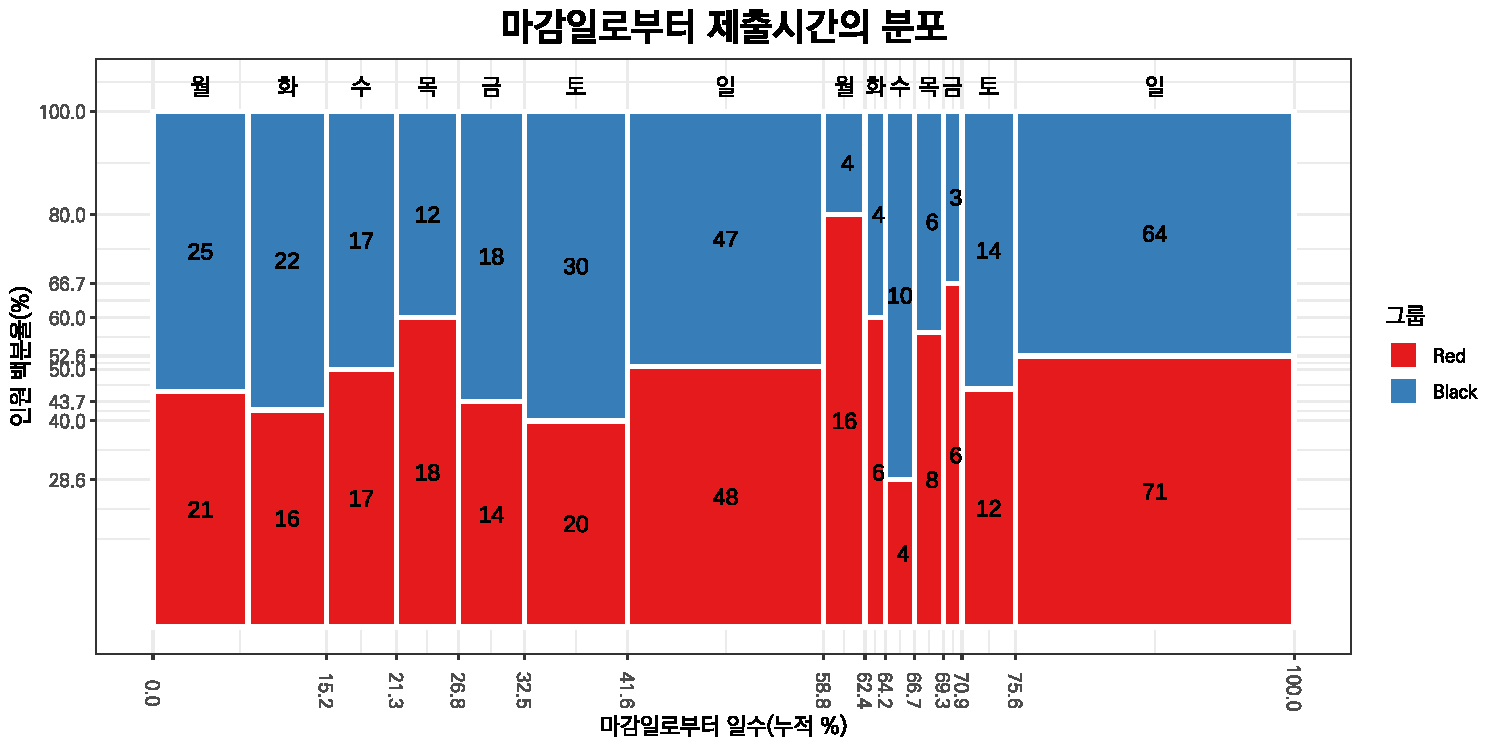
\includegraphics[keepaspectratio]{Quiz_report_2025_files/figure-latex/unnamed-chunk-65-1.pdf}}

\chapter{4주차 데이터 실험 집계}\label{uxc8fcuxcc28-uxb370uxc774uxd130-uxc2e4uxd5d8-uxc9d1uxacc4-3}

\section{실험의 목적}\label{uxc2e4uxd5d8uxc758-uxbaa9uxc801-3}

4주차 구글 예습 설문지 집계결과를 분석합니다.

Q1\textasciitilde Q6에서는 랜덤화의 효과로 Red, Black 이 얼마나 닮았는지 알아봅니다.

Q7에서는 부연설명을 어느 쪽에 붙이느냐에 따라서 Red 와 Black 의 응답이 달라지는 것을 알아봅니다.

끝으로 제출시간의 분포가 날마다 고른지, Red, Black 간에는 닮았는지 알아봅니다.

\subsection{Red, Black을 잘못 표시한 사람들}\label{red-blackuxc744-uxc798uxbabb-uxd45cuxc2dcuxd55c-uxc0acuxb78cuxb4e4-3}

\begin{longtable}[]{@{}
  >{\raggedright\arraybackslash}p{(\linewidth - 4\tabcolsep) * \real{0.3611}}
  >{\centering\arraybackslash}p{(\linewidth - 4\tabcolsep) * \real{0.2778}}
  >{\centering\arraybackslash}p{(\linewidth - 4\tabcolsep) * \real{0.3056}}@{}}
\toprule\noalign{}
\begin{minipage}[b]{\linewidth}\raggedright
~
\end{minipage} & \begin{minipage}[b]{\linewidth}\centering
Red(구글예습퀴즈)
\end{minipage} & \begin{minipage}[b]{\linewidth}\centering
Black(구글예습퀴즈)
\end{minipage} \\
\midrule\noalign{}
\endhead
\bottomrule\noalign{}
\endlastfoot
\textbf{Red(랜덤화출석부)} & 275 & 1 \\
\textbf{Black(랜덤화출석부)} & 3 & 285 \\
\textbf{계} & 278 & 286 \\
\end{longtable}

랜덤화출석부에 있는 Red, Black 과 실제 구글설문에 올린 Red, Black 이 다른 사람들의 수효는 4명입니다.

Red를 Black 이라고 한 사람이 1명, Black 을 Red 라고 한 사람이 3명입니다.

두 가지 방법으로 분석합니다.

우선 Red, Black 을 잘못 선택한 4명을 랜덤하게 둘로 나누면 어느 한 쪽 집단에 들어갈 기대인원은 4명을 둘로 나눈 2(명)이고, 표준오차는 4의 제곱근에 1/2을 곱해 준 1명이 됩니다.

실제로 Red를 Black 이라고 한 사람수, 1명이나 Black 을 Red 라고 한 사람수, 3명은 기대인원으로부터 표준오차 범위, 혹은 표준오차 두 배 범위에는 잘 들어갑니다.

두 번째 분석 방법은 확률을 계산해 보는 것입니다.

Red, Black 을 잘못 선택한 4명을 랜덤하게 둘로 나눌 때, 실제로 관찰된 3명 이상이나 1명이하로 잘못 선택한 사람수가 나올 가능성은 얼마나 되는가 입니다.

이 경우 공평한 동전던지기를 확률 법칙으로 표현한 이항분포로부터 계산할 수 있습니다.

시행횟수가 4이고 한 번 시행에서 성공확률이 1/2 인 이항분포에서 성공횟수가 1이하이거나 3이상을 관찰할 확률은 0.625입니다.

공평한 동전 던지기에서 앞면이 1개 이하 나오는 확률은 3개 이상 나오는 확률과 같기 때문에 사실상 한쪽만 계산해서 2배 해 주면 됩니다.

이 값을 p-value 라고 하는데, p-value가 0.05보다 작을 때 \textbf{통계적으로 유의한 차이를 관찰}하였다고 말합니다.

즉, 공평한 동전을 던지는 것과 같은 과정이라고 가정하였을 때 실제로 관찰된 값들이 가정으로부터 얼마나 떨어져 있는지를 표현한 것입니다.

0.05는 이런 실험을 스무 번 정도 반복하면 1번 나올 정도로 드문 사건을 의미합니다.

즉 가정이 잘못되었다는 것입니다.

그런데 Red, Black 을 잘못 표시한 사람들의 분포에서 관찰된 p-value 는 0.05와는 비교도 안될 정도로 큰 값입니다.

따라서 두 집단이 랜덤화 효과가 작동하여 \textbf{통계적으로 유의한 차이를 보이지 않는다}고 할 수 있습니다.

\subsection{응답인원의 Red, Black}\label{uxc751uxb2f5uxc778uxc6d0uxc758-red-black-3}

Red 로 응답한 인원은 278명, Black 에 응답한 인원은 286명입니다.

전체 응답인원 564 명을 랜덤하게 둘로 나눌 때 어느 한 쪽의 기대인원은 전체 응답인원의 절반인 282명이고, 표준오차는 전체 응답인원의 제곱근에 1/2을 곱해 준 11.9 명입니다.

따라서 Red, Black 각 그룹에 관찰된 인원은 기대인원으로부터 표준오차 범위, 혹은 2배의 표준오차 범위 안에 들어갑니다.

\section{Q1. 세종대왕 시대 조세제도}\label{q1.-uxc138uxc885uxb300uxc655-uxc2dcuxb300-uxc870uxc138uxc81cuxb3c4}

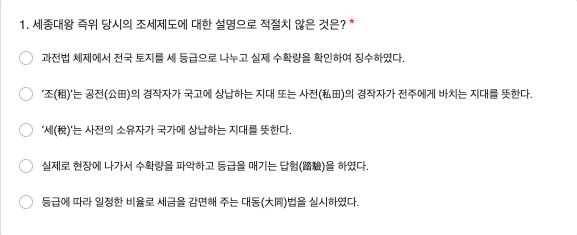
\includegraphics[width=0.75\linewidth]{./pics/Quiz230322_Q1}

\subsection{조선초기 조세제도}\label{uxc870uxc120uxcd08uxae30-uxc870uxc138uxc81cuxb3c4}

\begin{longtable}[]{@{}
  >{\raggedright\arraybackslash}p{(\linewidth - 12\tabcolsep) * \real{0.0674}}
  >{\centering\arraybackslash}p{(\linewidth - 12\tabcolsep) * \real{0.1854}}
  >{\centering\arraybackslash}p{(\linewidth - 12\tabcolsep) * \real{0.1854}}
  >{\centering\arraybackslash}p{(\linewidth - 12\tabcolsep) * \real{0.1854}}
  >{\centering\arraybackslash}p{(\linewidth - 12\tabcolsep) * \real{0.1798}}
  >{\centering\arraybackslash}p{(\linewidth - 12\tabcolsep) * \real{0.1629}}
  >{\centering\arraybackslash}p{(\linewidth - 12\tabcolsep) * \real{0.0337}}@{}}
\toprule\noalign{}
\begin{minipage}[b]{\linewidth}\raggedright
~
\end{minipage} & \begin{minipage}[b]{\linewidth}\centering
과전법 체제에서 전국 토지를 세
등급으로 나누고 실제 수확량을
확인하여 징수하였다.
\end{minipage} & \begin{minipage}[b]{\linewidth}\centering
'조(租)'는 공전(公田)의
경작자가 국고에 상납하는 지대
또는 사전(私田)의 경작자가
전주에게 바치는 지대를 뜻한다.
\end{minipage} & \begin{minipage}[b]{\linewidth}\centering
'세(稅)'는 사전의 소유자가
국가에 상납하는 지세를 뜻한다.
\end{minipage} & \begin{minipage}[b]{\linewidth}\centering
실제로 현장에 나가서 수확량을
파악하고 등급을 매기는
답험(踏驗)을 하였다.
\end{minipage} & \begin{minipage}[b]{\linewidth}\centering
등급에 따라 일정한 비율로
세금을 감면해 주는
대동(大同)법을 실시하였다.
\end{minipage} & \begin{minipage}[b]{\linewidth}\centering
계
\end{minipage} \\
\midrule\noalign{}
\endhead
\bottomrule\noalign{}
\endlastfoot
\textbf{Red} & 22 & 28 & 26 & 22 & 180 & 278 \\
\textbf{Black} & 17 & 30 & 17 & 19 & 203 & 286 \\
\textbf{계} & 39 & 58 & 43 & 41 & 383 & 564 \\
\end{longtable}

\begin{longtable}[]{@{}
  >{\raggedleft\arraybackslash}p{(\linewidth - 4\tabcolsep) * \real{0.2361}}
  >{\raggedleft\arraybackslash}p{(\linewidth - 4\tabcolsep) * \real{0.0694}}
  >{\raggedleft\arraybackslash}p{(\linewidth - 4\tabcolsep) * \real{0.1389}}@{}}
\caption{Pearson's Chi-squared test: \texttt{.}}\tabularnewline
\toprule\noalign{}
\begin{minipage}[b]{\linewidth}\raggedleft
Test statistic
\end{minipage} & \begin{minipage}[b]{\linewidth}\raggedleft
df
\end{minipage} & \begin{minipage}[b]{\linewidth}\raggedleft
P value
\end{minipage} \\
\midrule\noalign{}
\endfirsthead
\toprule\noalign{}
\begin{minipage}[b]{\linewidth}\raggedleft
Test statistic
\end{minipage} & \begin{minipage}[b]{\linewidth}\raggedleft
df
\end{minipage} & \begin{minipage}[b]{\linewidth}\raggedleft
P value
\end{minipage} \\
\midrule\noalign{}
\endhead
\bottomrule\noalign{}
\endlastfoot
4.082 & 4 & 0.3951 \\
\end{longtable}

Q1의 집계 결과가 Red, Black 간에 통계적으로 유의한 차이가 있는지 알아보기 위하여 카이제곱 테스트를 수행하였습니다.

그 결과 카이제곱 통계량은 4.08, 자유도는 4 , p-value 는 0.3951이므로 Red, Black 간에 통계적으로 유의한 차이를 보이지 않습니다.

실제로 닮은 게 느껴집니까?

\subsection{조선초기 조세제도(\%)}\label{uxc870uxc120uxcd08uxae30-uxc870uxc138uxc81cuxb3c4-1}

\begin{longtable}[]{@{}
  >{\centering\arraybackslash}p{(\linewidth - 10\tabcolsep) * \real{0.1964}}
  >{\centering\arraybackslash}p{(\linewidth - 10\tabcolsep) * \real{0.1964}}
  >{\centering\arraybackslash}p{(\linewidth - 10\tabcolsep) * \real{0.1964}}
  >{\centering\arraybackslash}p{(\linewidth - 10\tabcolsep) * \real{0.1905}}
  >{\centering\arraybackslash}p{(\linewidth - 10\tabcolsep) * \real{0.1726}}
  >{\centering\arraybackslash}p{(\linewidth - 10\tabcolsep) * \real{0.0476}}@{}}
\toprule\noalign{}
\begin{minipage}[b]{\linewidth}\centering
과전법 체제에서 전국 토지를 세
등급으로 나누고 실제 수확량을
확인하여 징수하였다.
\end{minipage} & \begin{minipage}[b]{\linewidth}\centering
'조(租)'는 공전(公田)의
경작자가 국고에 상납하는 지대
또는 사전(私田)의 경작자가
전주에게 바치는 지대를 뜻한다.
\end{minipage} & \begin{minipage}[b]{\linewidth}\centering
'세(稅)'는 사전의 소유자가
국가에 상납하는 지세를 뜻한다.
\end{minipage} & \begin{minipage}[b]{\linewidth}\centering
실제로 현장에 나가서 수확량을
파악하고 등급을 매기는
답험(踏驗)을 하였다.
\end{minipage} & \begin{minipage}[b]{\linewidth}\centering
등급에 따라 일정한 비율로
세금을 감면해 주는
대동(大同)법을 실시하였다.
\end{minipage} & \begin{minipage}[b]{\linewidth}\centering
계
\end{minipage} \\
\midrule\noalign{}
\endhead
\bottomrule\noalign{}
\endlastfoot
6.9 & 10.3 & 7.6 & 7.3 & 67.9 & 100.0 \\
\end{longtable}

정답률은 Red, Black 을 합하여 계산하는데, 67.9(\%) 입니다.

\section{Q2. 공법도입에 대한 대신들의 찬성율}\label{q2.-uxacf5uxbc95uxb3c4uxc785uxc5d0-uxb300uxd55c-uxb300uxc2e0uxb4e4uxc758-uxcc2cuxc131uxc728}

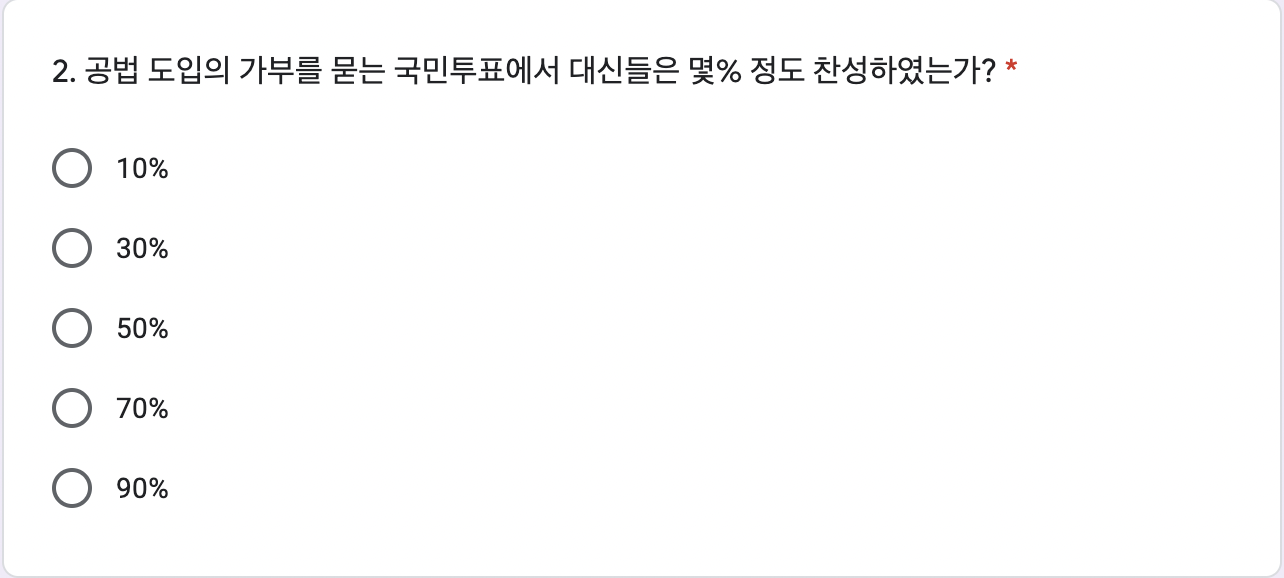
\includegraphics[width=0.75\linewidth]{./pics/Quiz210913_Q2}

\subsection{공법도입과 대신들(집계표)}\label{uxacf5uxbc95uxb3c4uxc785uxacfc-uxb300uxc2e0uxb4e4uxc9d1uxacc4uxd45c}

\begin{longtable}[]{@{}
  >{\raggedright\arraybackslash}p{(\linewidth - 12\tabcolsep) * \real{0.1667}}
  >{\raggedleft\arraybackslash}p{(\linewidth - 12\tabcolsep) * \real{0.0833}}
  >{\raggedleft\arraybackslash}p{(\linewidth - 12\tabcolsep) * \real{0.0833}}
  >{\raggedleft\arraybackslash}p{(\linewidth - 12\tabcolsep) * \real{0.0833}}
  >{\raggedleft\arraybackslash}p{(\linewidth - 12\tabcolsep) * \real{0.0833}}
  >{\raggedleft\arraybackslash}p{(\linewidth - 12\tabcolsep) * \real{0.0833}}
  >{\centering\arraybackslash}p{(\linewidth - 12\tabcolsep) * \real{0.0833}}@{}}
\toprule\noalign{}
\begin{minipage}[b]{\linewidth}\raggedright
~
\end{minipage} & \begin{minipage}[b]{\linewidth}\raggedleft
10\%
\end{minipage} & \begin{minipage}[b]{\linewidth}\raggedleft
30\%
\end{minipage} & \begin{minipage}[b]{\linewidth}\raggedleft
50\%
\end{minipage} & \begin{minipage}[b]{\linewidth}\raggedleft
70\%
\end{minipage} & \begin{minipage}[b]{\linewidth}\raggedleft
90\%
\end{minipage} & \begin{minipage}[b]{\linewidth}\centering
계
\end{minipage} \\
\midrule\noalign{}
\endhead
\bottomrule\noalign{}
\endlastfoot
\textbf{Red} & 153 & 54 & 28 & 27 & 16 & 278 \\
\textbf{Black} & 160 & 46 & 26 & 32 & 22 & 286 \\
\textbf{계} & 313 & 100 & 54 & 59 & 38 & 564 \\
\end{longtable}

\begin{longtable}[]{@{}
  >{\raggedleft\arraybackslash}p{(\linewidth - 4\tabcolsep) * \real{0.2361}}
  >{\raggedleft\arraybackslash}p{(\linewidth - 4\tabcolsep) * \real{0.0694}}
  >{\raggedleft\arraybackslash}p{(\linewidth - 4\tabcolsep) * \real{0.1389}}@{}}
\caption{Pearson's Chi-squared test: \texttt{.}}\tabularnewline
\toprule\noalign{}
\begin{minipage}[b]{\linewidth}\raggedleft
Test statistic
\end{minipage} & \begin{minipage}[b]{\linewidth}\raggedleft
df
\end{minipage} & \begin{minipage}[b]{\linewidth}\raggedleft
P value
\end{minipage} \\
\midrule\noalign{}
\endfirsthead
\toprule\noalign{}
\begin{minipage}[b]{\linewidth}\raggedleft
Test statistic
\end{minipage} & \begin{minipage}[b]{\linewidth}\raggedleft
df
\end{minipage} & \begin{minipage}[b]{\linewidth}\raggedleft
P value
\end{minipage} \\
\midrule\noalign{}
\endhead
\bottomrule\noalign{}
\endlastfoot
2.129 & 4 & 0.7121 \\
\end{longtable}

Q2의 집계 결과가 Red, Black 간에 통계적으로 유의한 차이가 있는지 알아보기 위하여 카이제곱 테스트를 수행하였습니다.

그 결과 카이제곱 통계량은 2.129, 자유도는 4, p-value 는 0.7121이므로 Red, Black 간에 통계적으로 유의한 차이를 보이지 않습니다.

실제로 닮은 게 느껴집니까?

\subsection{공법도입과 대신들(\%)}\label{uxacf5uxbc95uxb3c4uxc785uxacfc-uxb300uxc2e0uxb4e4}

\begin{longtable}[]{@{}
  >{\raggedleft\arraybackslash}p{(\linewidth - 10\tabcolsep) * \real{0.0972}}
  >{\raggedleft\arraybackslash}p{(\linewidth - 10\tabcolsep) * \real{0.0972}}
  >{\raggedleft\arraybackslash}p{(\linewidth - 10\tabcolsep) * \real{0.0833}}
  >{\raggedleft\arraybackslash}p{(\linewidth - 10\tabcolsep) * \real{0.0972}}
  >{\raggedleft\arraybackslash}p{(\linewidth - 10\tabcolsep) * \real{0.0833}}
  >{\centering\arraybackslash}p{(\linewidth - 10\tabcolsep) * \real{0.1111}}@{}}
\toprule\noalign{}
\begin{minipage}[b]{\linewidth}\raggedleft
10\%
\end{minipage} & \begin{minipage}[b]{\linewidth}\raggedleft
30\%
\end{minipage} & \begin{minipage}[b]{\linewidth}\raggedleft
50\%
\end{minipage} & \begin{minipage}[b]{\linewidth}\raggedleft
70\%
\end{minipage} & \begin{minipage}[b]{\linewidth}\raggedleft
90\%
\end{minipage} & \begin{minipage}[b]{\linewidth}\centering
계
\end{minipage} \\
\midrule\noalign{}
\endhead
\bottomrule\noalign{}
\endlastfoot
55.5 & 17.7 & 9.6 & 10.5 & 6.7 & 100.0 \\
\end{longtable}

정답률은 Red, Black 을 합하여 계산하는데, 55.5(\%) 입니다.

\section{Q3. 공법도입과 품관촌민들의 찬반}\label{q3.-uxacf5uxbc95uxb3c4uxc785uxacfc-uxd488uxad00uxcd0cuxbbfcuxb4e4uxc758-uxcc2cuxbc18}

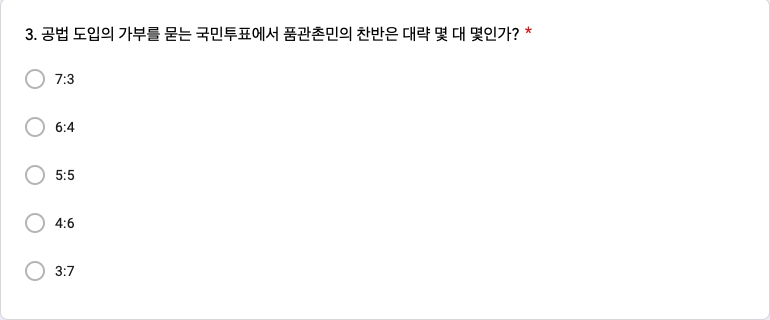
\includegraphics[width=0.75\linewidth]{./pics/Quiz210316_Q3}

\subsection{품관촌민들의 찬반(집계표)}\label{uxd488uxad00uxcd0cuxbbfcuxb4e4uxc758-uxcc2cuxbc18uxc9d1uxacc4uxd45c}

\begin{longtable}[]{@{}
  >{\raggedright\arraybackslash}p{(\linewidth - 12\tabcolsep) * \real{0.1667}}
  >{\raggedleft\arraybackslash}p{(\linewidth - 12\tabcolsep) * \real{0.0833}}
  >{\raggedleft\arraybackslash}p{(\linewidth - 12\tabcolsep) * \real{0.0833}}
  >{\raggedleft\arraybackslash}p{(\linewidth - 12\tabcolsep) * \real{0.0833}}
  >{\raggedleft\arraybackslash}p{(\linewidth - 12\tabcolsep) * \real{0.0833}}
  >{\raggedleft\arraybackslash}p{(\linewidth - 12\tabcolsep) * \real{0.0833}}
  >{\centering\arraybackslash}p{(\linewidth - 12\tabcolsep) * \real{0.0833}}@{}}
\toprule\noalign{}
\begin{minipage}[b]{\linewidth}\raggedright
~
\end{minipage} & \begin{minipage}[b]{\linewidth}\raggedleft
7:3
\end{minipage} & \begin{minipage}[b]{\linewidth}\raggedleft
6:4
\end{minipage} & \begin{minipage}[b]{\linewidth}\raggedleft
5:5
\end{minipage} & \begin{minipage}[b]{\linewidth}\raggedleft
4:6
\end{minipage} & \begin{minipage}[b]{\linewidth}\raggedleft
3:7
\end{minipage} & \begin{minipage}[b]{\linewidth}\centering
계
\end{minipage} \\
\midrule\noalign{}
\endhead
\bottomrule\noalign{}
\endlastfoot
\textbf{Red} & 48 & 159 & 25 & 22 & 24 & 278 \\
\textbf{Black} & 62 & 162 & 25 & 18 & 19 & 286 \\
\textbf{계} & 110 & 321 & 50 & 40 & 43 & 564 \\
\end{longtable}

\begin{longtable}[]{@{}
  >{\raggedleft\arraybackslash}p{(\linewidth - 4\tabcolsep) * \real{0.2361}}
  >{\raggedleft\arraybackslash}p{(\linewidth - 4\tabcolsep) * \real{0.0694}}
  >{\raggedleft\arraybackslash}p{(\linewidth - 4\tabcolsep) * \real{0.1389}}@{}}
\caption{Pearson's Chi-squared test: \texttt{.}}\tabularnewline
\toprule\noalign{}
\begin{minipage}[b]{\linewidth}\raggedleft
Test statistic
\end{minipage} & \begin{minipage}[b]{\linewidth}\raggedleft
df
\end{minipage} & \begin{minipage}[b]{\linewidth}\raggedleft
P value
\end{minipage} \\
\midrule\noalign{}
\endfirsthead
\toprule\noalign{}
\begin{minipage}[b]{\linewidth}\raggedleft
Test statistic
\end{minipage} & \begin{minipage}[b]{\linewidth}\raggedleft
df
\end{minipage} & \begin{minipage}[b]{\linewidth}\raggedleft
P value
\end{minipage} \\
\midrule\noalign{}
\endhead
\bottomrule\noalign{}
\endlastfoot
2.678 & 4 & 0.613 \\
\end{longtable}

Q3의 집계 결과가 Red, Black 간에 통계적으로 유의한 차이가 있는지 알아보기 위하여 카이제곱 테스트를 수행하였습니다.

그 결과 카이제곱 통계량은 2.678, 자유도는 4, p-value 는 0.6130이므로 Red, Black 간에 통계적으로 유의한 차이를 보이지 않습니다.

실제로 닮은 게 느껴집니까?

\subsection{품관촌민들의 찬반(\%)}\label{uxd488uxad00uxcd0cuxbbfcuxb4e4uxc758-uxcc2cuxbc18}

\begin{longtable}[]{@{}
  >{\raggedleft\arraybackslash}p{(\linewidth - 10\tabcolsep) * \real{0.0972}}
  >{\raggedleft\arraybackslash}p{(\linewidth - 10\tabcolsep) * \real{0.0972}}
  >{\raggedleft\arraybackslash}p{(\linewidth - 10\tabcolsep) * \real{0.0833}}
  >{\raggedleft\arraybackslash}p{(\linewidth - 10\tabcolsep) * \real{0.0833}}
  >{\raggedleft\arraybackslash}p{(\linewidth - 10\tabcolsep) * \real{0.0833}}
  >{\centering\arraybackslash}p{(\linewidth - 10\tabcolsep) * \real{0.1111}}@{}}
\toprule\noalign{}
\begin{minipage}[b]{\linewidth}\raggedleft
7:3
\end{minipage} & \begin{minipage}[b]{\linewidth}\raggedleft
6:4
\end{minipage} & \begin{minipage}[b]{\linewidth}\raggedleft
5:5
\end{minipage} & \begin{minipage}[b]{\linewidth}\raggedleft
4:6
\end{minipage} & \begin{minipage}[b]{\linewidth}\raggedleft
3:7
\end{minipage} & \begin{minipage}[b]{\linewidth}\centering
계
\end{minipage} \\
\midrule\noalign{}
\endhead
\bottomrule\noalign{}
\endlastfoot
19.5 & 56.9 & 8.9 & 7.1 & 7.6 & 100.0 \\
\end{longtable}

정답률은 Red, Black 을 합하여 계산하는데, 56.9(\%) 입니다.

\section{Q4. 공법}\label{q4.-uxacf5uxbc95}

\begin{flushleft}
\includegraphics[width=0.75\linewidth]{./pics/Quiz210316_Q4} \end{flushleft}

\subsection{기본세율}\label{uxae30uxbcf8uxc138uxc728}

\begin{longtable}[]{@{}
  >{\raggedright\arraybackslash}p{(\linewidth - 10\tabcolsep) * \real{0.1667}}
  >{\raggedleft\arraybackslash}p{(\linewidth - 10\tabcolsep) * \real{0.0972}}
  >{\raggedleft\arraybackslash}p{(\linewidth - 10\tabcolsep) * \real{0.0972}}
  >{\raggedleft\arraybackslash}p{(\linewidth - 10\tabcolsep) * \real{0.0972}}
  >{\raggedleft\arraybackslash}p{(\linewidth - 10\tabcolsep) * \real{0.0972}}
  >{\centering\arraybackslash}p{(\linewidth - 10\tabcolsep) * \real{0.0972}}@{}}
\toprule\noalign{}
\begin{minipage}[b]{\linewidth}\raggedright
~
\end{minipage} & \begin{minipage}[b]{\linewidth}\raggedleft
1/10
\end{minipage} & \begin{minipage}[b]{\linewidth}\raggedleft
1/15
\end{minipage} & \begin{minipage}[b]{\linewidth}\raggedleft
1/20
\end{minipage} & \begin{minipage}[b]{\linewidth}\raggedleft
1/30
\end{minipage} & \begin{minipage}[b]{\linewidth}\centering
계
\end{minipage} \\
\midrule\noalign{}
\endhead
\bottomrule\noalign{}
\endlastfoot
\textbf{Red} & 84 & 47 & 132 & 15 & 278 \\
\textbf{Black} & 88 & 29 & 154 & 15 & 286 \\
\textbf{계} & 172 & 76 & 286 & 30 & 564 \\
\end{longtable}

\begin{longtable}[]{@{}
  >{\raggedleft\arraybackslash}p{(\linewidth - 4\tabcolsep) * \real{0.2361}}
  >{\raggedleft\arraybackslash}p{(\linewidth - 4\tabcolsep) * \real{0.0694}}
  >{\raggedleft\arraybackslash}p{(\linewidth - 4\tabcolsep) * \real{0.1389}}@{}}
\caption{Pearson's Chi-squared test: \texttt{.}}\tabularnewline
\toprule\noalign{}
\begin{minipage}[b]{\linewidth}\raggedleft
Test statistic
\end{minipage} & \begin{minipage}[b]{\linewidth}\raggedleft
df
\end{minipage} & \begin{minipage}[b]{\linewidth}\raggedleft
P value
\end{minipage} \\
\midrule\noalign{}
\endfirsthead
\toprule\noalign{}
\begin{minipage}[b]{\linewidth}\raggedleft
Test statistic
\end{minipage} & \begin{minipage}[b]{\linewidth}\raggedleft
df
\end{minipage} & \begin{minipage}[b]{\linewidth}\raggedleft
P value
\end{minipage} \\
\midrule\noalign{}
\endhead
\bottomrule\noalign{}
\endlastfoot
5.936 & 3 & 0.1148 \\
\end{longtable}

Q4의 집계 결과가 Red, Black 간에 통계적으로 유의한 차이가 있는지 알아보기 위하여 카이제곱 테스트를 수행하였습니다.

그 결과 카이제곱 통계량은 5.936, 자유도는 3, p-value 는 0.1148이므로 Red, Black 간에 통계적으로 유의한 차이를 보이지 않습니다.

실제로 닮은 게 느껴집니까?

\subsection{기본세율(\%)}\label{uxae30uxbcf8uxc138uxc728-1}

\begin{longtable}[]{@{}
  >{\raggedleft\arraybackslash}p{(\linewidth - 8\tabcolsep) * \real{0.0972}}
  >{\raggedleft\arraybackslash}p{(\linewidth - 8\tabcolsep) * \real{0.0972}}
  >{\raggedleft\arraybackslash}p{(\linewidth - 8\tabcolsep) * \real{0.0972}}
  >{\raggedleft\arraybackslash}p{(\linewidth - 8\tabcolsep) * \real{0.0972}}
  >{\centering\arraybackslash}p{(\linewidth - 8\tabcolsep) * \real{0.1111}}@{}}
\toprule\noalign{}
\begin{minipage}[b]{\linewidth}\raggedleft
1/10
\end{minipage} & \begin{minipage}[b]{\linewidth}\raggedleft
1/15
\end{minipage} & \begin{minipage}[b]{\linewidth}\raggedleft
1/20
\end{minipage} & \begin{minipage}[b]{\linewidth}\raggedleft
1/30
\end{minipage} & \begin{minipage}[b]{\linewidth}\centering
계
\end{minipage} \\
\midrule\noalign{}
\endhead
\bottomrule\noalign{}
\endlastfoot
30.5 & 13.5 & 50.7 & 5.3 & 100.0 \\
\end{longtable}

정답률은 Red, Black 을 합하여 계산하는데, 30.5(\%) 입니다.

\section{Q5. 1423년 조선시대 호구와 인구}\label{q5.-1423uxb144-uxc870uxc120uxc2dcuxb300-uxd638uxad6cuxc640-uxc778uxad6c}

\begin{flushleft}
\includegraphics[width=0.75\linewidth]{./pics/Quiz210316_Q5} \end{flushleft}

\subsection{호구와 인구}\label{uxd638uxad6cuxc640-uxc778uxad6c}

\begin{longtable}[]{@{}
  >{\raggedright\arraybackslash}p{(\linewidth - 10\tabcolsep) * \real{0.1667}}
  >{\centering\arraybackslash}p{(\linewidth - 10\tabcolsep) * \real{0.1250}}
  >{\centering\arraybackslash}p{(\linewidth - 10\tabcolsep) * \real{0.1250}}
  >{\centering\arraybackslash}p{(\linewidth - 10\tabcolsep) * \real{0.1250}}
  >{\centering\arraybackslash}p{(\linewidth - 10\tabcolsep) * \real{0.1389}}
  >{\centering\arraybackslash}p{(\linewidth - 10\tabcolsep) * \real{0.0833}}@{}}
\toprule\noalign{}
\begin{minipage}[b]{\linewidth}\raggedright
~
\end{minipage} & \begin{minipage}[b]{\linewidth}\centering
15만호
\end{minipage} & \begin{minipage}[b]{\linewidth}\centering
20만호
\end{minipage} & \begin{minipage}[b]{\linewidth}\centering
44만호
\end{minipage} & \begin{minipage}[b]{\linewidth}\centering
130만호
\end{minipage} & \begin{minipage}[b]{\linewidth}\centering
계
\end{minipage} \\
\midrule\noalign{}
\endhead
\bottomrule\noalign{}
\endlastfoot
\textbf{Red} & 11 & 164 & 87 & 16 & 278 \\
\textbf{Black} & 22 & 151 & 105 & 8 & 286 \\
\textbf{계} & 33 & 315 & 192 & 24 & 564 \\
\end{longtable}

\begin{longtable}[]{@{}
  >{\raggedleft\arraybackslash}p{(\linewidth - 4\tabcolsep) * \real{0.2361}}
  >{\raggedleft\arraybackslash}p{(\linewidth - 4\tabcolsep) * \real{0.0694}}
  >{\raggedleft\arraybackslash}p{(\linewidth - 4\tabcolsep) * \real{0.1667}}@{}}
\caption{Pearson's Chi-squared test: \texttt{.}}\tabularnewline
\toprule\noalign{}
\begin{minipage}[b]{\linewidth}\raggedleft
Test statistic
\end{minipage} & \begin{minipage}[b]{\linewidth}\raggedleft
df
\end{minipage} & \begin{minipage}[b]{\linewidth}\raggedleft
P value
\end{minipage} \\
\midrule\noalign{}
\endfirsthead
\toprule\noalign{}
\begin{minipage}[b]{\linewidth}\raggedleft
Test statistic
\end{minipage} & \begin{minipage}[b]{\linewidth}\raggedleft
df
\end{minipage} & \begin{minipage}[b]{\linewidth}\raggedleft
P value
\end{minipage} \\
\midrule\noalign{}
\endhead
\bottomrule\noalign{}
\endlastfoot
8.446 & 3 & 0.03765 * \\
\end{longtable}

Q5의 집계 결과가 Red, Black 간에 통계적으로 유의한 차이가 있는지 알아보기 위하여 카이제곱 테스트를 수행하였습니다.

그 결과 카이제곱 통계량은 8.446, 자유도는 3, p-value 는 0.0376이므로 Red, Black 간에 통계적으로 유의한 차이를 보이고 있습니다.

\subsection{호구와 인구(\%)}\label{uxd638uxad6cuxc640-uxc778uxad6c-1}

\begin{longtable}[]{@{}
  >{\centering\arraybackslash}p{(\linewidth - 8\tabcolsep) * \real{0.1250}}
  >{\centering\arraybackslash}p{(\linewidth - 8\tabcolsep) * \real{0.1250}}
  >{\centering\arraybackslash}p{(\linewidth - 8\tabcolsep) * \real{0.1250}}
  >{\centering\arraybackslash}p{(\linewidth - 8\tabcolsep) * \real{0.1389}}
  >{\centering\arraybackslash}p{(\linewidth - 8\tabcolsep) * \real{0.1389}}@{}}
\toprule\noalign{}
\begin{minipage}[b]{\linewidth}\centering
15만호
\end{minipage} & \begin{minipage}[b]{\linewidth}\centering
20만호
\end{minipage} & \begin{minipage}[b]{\linewidth}\centering
44만호
\end{minipage} & \begin{minipage}[b]{\linewidth}\centering
130만호
\end{minipage} & \begin{minipage}[b]{\linewidth}\centering
계
\end{minipage} \\
\midrule\noalign{}
\endhead
\bottomrule\noalign{}
\endlastfoot
5.9 & 55.9 & 34.0 & 4.3 & 100.0 \\
\end{longtable}

정답률은 Red, Black 을 합하여 계산하는데, 55.9(\%) 입니다.

\section{Q6. 지방관료와 품관촌민}\label{q6.-uxc9c0uxbc29uxad00uxb8ccuxc640-uxd488uxad00uxcd0cuxbbfc}

\begin{flushleft}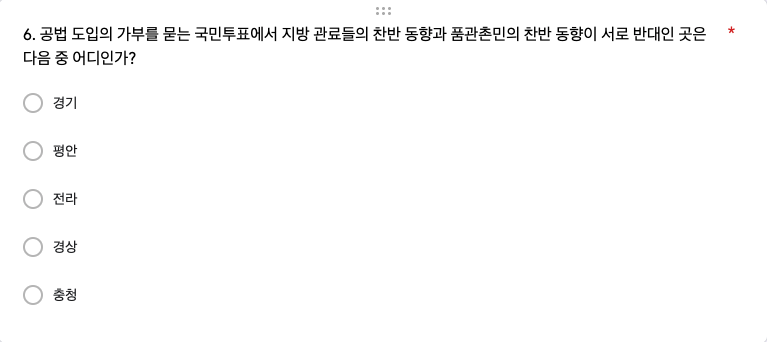
\includegraphics[width=0.75\linewidth]{./pics/Quiz210316_Q6} \end{flushleft}

\subsection{찬반이 반대인 곳(집계표)}\label{uxcc2cuxbc18uxc774-uxbc18uxb300uxc778-uxacf3uxc9d1uxacc4uxd45c}

\begin{longtable}[]{@{}
  >{\raggedright\arraybackslash}p{(\linewidth - 12\tabcolsep) * \real{0.1667}}
  >{\centering\arraybackslash}p{(\linewidth - 12\tabcolsep) * \real{0.0972}}
  >{\centering\arraybackslash}p{(\linewidth - 12\tabcolsep) * \real{0.0972}}
  >{\centering\arraybackslash}p{(\linewidth - 12\tabcolsep) * \real{0.0972}}
  >{\centering\arraybackslash}p{(\linewidth - 12\tabcolsep) * \real{0.0972}}
  >{\centering\arraybackslash}p{(\linewidth - 12\tabcolsep) * \real{0.0972}}
  >{\centering\arraybackslash}p{(\linewidth - 12\tabcolsep) * \real{0.0972}}@{}}
\toprule\noalign{}
\begin{minipage}[b]{\linewidth}\raggedright
~
\end{minipage} & \begin{minipage}[b]{\linewidth}\centering
경기
\end{minipage} & \begin{minipage}[b]{\linewidth}\centering
평안
\end{minipage} & \begin{minipage}[b]{\linewidth}\centering
전라
\end{minipage} & \begin{minipage}[b]{\linewidth}\centering
경상
\end{minipage} & \begin{minipage}[b]{\linewidth}\centering
충청
\end{minipage} & \begin{minipage}[b]{\linewidth}\centering
계
\end{minipage} \\
\midrule\noalign{}
\endhead
\bottomrule\noalign{}
\endlastfoot
\textbf{Red} & 25 & 39 & 44 & 40 & 130 & 278 \\
\textbf{Black} & 25 & 37 & 51 & 43 & 130 & 286 \\
\textbf{계} & 50 & 76 & 95 & 83 & 260 & 564 \\
\end{longtable}

\begin{longtable}[]{@{}
  >{\raggedleft\arraybackslash}p{(\linewidth - 4\tabcolsep) * \real{0.2361}}
  >{\raggedleft\arraybackslash}p{(\linewidth - 4\tabcolsep) * \real{0.0694}}
  >{\raggedleft\arraybackslash}p{(\linewidth - 4\tabcolsep) * \real{0.1389}}@{}}
\caption{Pearson's Chi-squared test: \texttt{.}}\tabularnewline
\toprule\noalign{}
\begin{minipage}[b]{\linewidth}\raggedleft
Test statistic
\end{minipage} & \begin{minipage}[b]{\linewidth}\raggedleft
df
\end{minipage} & \begin{minipage}[b]{\linewidth}\raggedleft
P value
\end{minipage} \\
\midrule\noalign{}
\endfirsthead
\toprule\noalign{}
\begin{minipage}[b]{\linewidth}\raggedleft
Test statistic
\end{minipage} & \begin{minipage}[b]{\linewidth}\raggedleft
df
\end{minipage} & \begin{minipage}[b]{\linewidth}\raggedleft
P value
\end{minipage} \\
\midrule\noalign{}
\endhead
\bottomrule\noalign{}
\endlastfoot
0.5635 & 4 & 0.967 \\
\end{longtable}

Q6의 집계 결과가 Red, Black 간에 통계적으로 유의한 차이가 있는지 알아보기 위하여 카이제곱 테스트를 수행하였습니다.

그 결과 카이제곱 통계량은 0.563, 자유도는 4, p-value 는 0.9670이므로 Red, Black 간에 통계적으로 유의한 차이를 보이지 않습니다.

실제로 닮은 게 느껴집니까?

\subsection{찬반이 반대인 곳(\%)}\label{uxcc2cuxbc18uxc774-uxbc18uxb300uxc778-uxacf3}

\begin{longtable}[]{@{}
  >{\centering\arraybackslash}p{(\linewidth - 10\tabcolsep) * \real{0.0972}}
  >{\centering\arraybackslash}p{(\linewidth - 10\tabcolsep) * \real{0.0972}}
  >{\centering\arraybackslash}p{(\linewidth - 10\tabcolsep) * \real{0.0972}}
  >{\centering\arraybackslash}p{(\linewidth - 10\tabcolsep) * \real{0.0972}}
  >{\centering\arraybackslash}p{(\linewidth - 10\tabcolsep) * \real{0.0972}}
  >{\centering\arraybackslash}p{(\linewidth - 10\tabcolsep) * \real{0.1111}}@{}}
\toprule\noalign{}
\begin{minipage}[b]{\linewidth}\centering
경기
\end{minipage} & \begin{minipage}[b]{\linewidth}\centering
평안
\end{minipage} & \begin{minipage}[b]{\linewidth}\centering
전라
\end{minipage} & \begin{minipage}[b]{\linewidth}\centering
경상
\end{minipage} & \begin{minipage}[b]{\linewidth}\centering
충청
\end{minipage} & \begin{minipage}[b]{\linewidth}\centering
계
\end{minipage} \\
\midrule\noalign{}
\endhead
\bottomrule\noalign{}
\endlastfoot
8.9 & 13.5 & 16.8 & 14.7 & 46.1 & 100.0 \\
\end{longtable}

정답률은 Red, Black 을 합하여 계산하는데, 46.1(\%) 입니다.

\section{Q7. 부연설명의 효과 : 주당 근로 69시간제 도입 찬반}\label{q7.-uxbd80uxc5f0uxc124uxba85uxc758-uxd6a8uxacfc-uxc8fcuxb2f9-uxadfcuxb85c-69uxc2dcuxac04uxc81c-uxb3c4uxc785-uxcc2cuxbc18}

부연설명을 찬성 쪽에 붙이는가(Red), 또는 반대 쪽에 붙이는가(Black)에 따라 응답이 영향을 받는 것으로 관찰됩니다.

찬반여부에 대한 카이제곱테스트의 p-value를 놓고 볼 때 그 차이가 통계적으로 매우 유의합니다.

\begin{flushleft}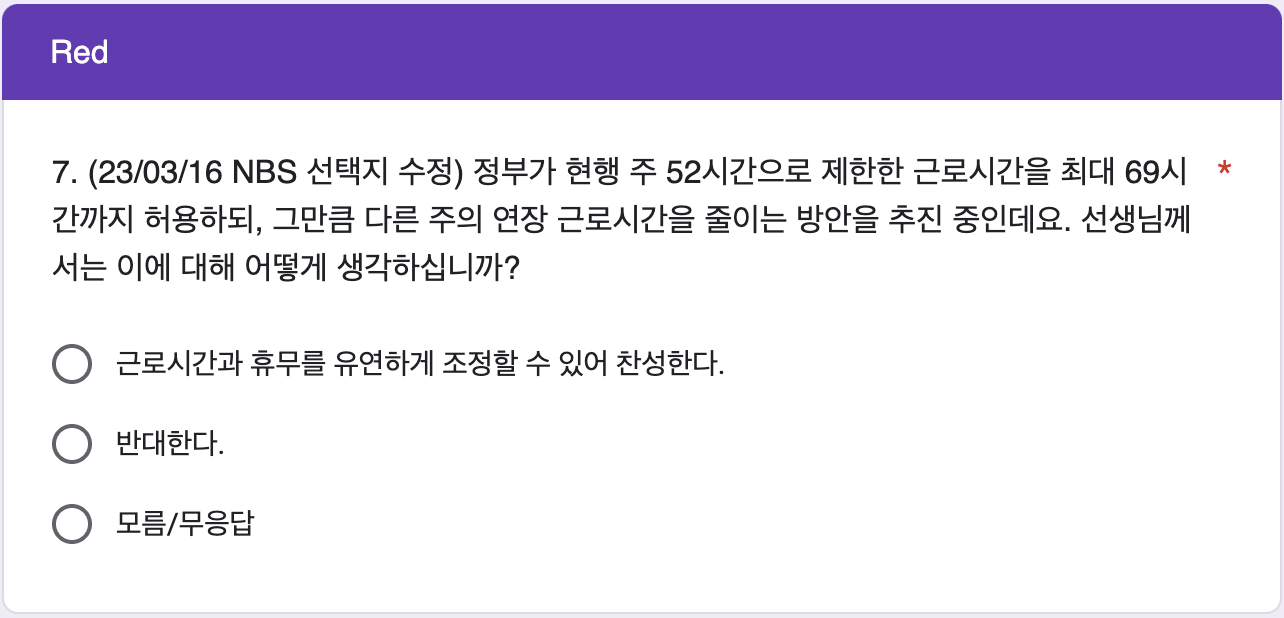
\includegraphics[width=0.67\linewidth]{./pics/Quiz240322_Q7_Red} \end{flushleft}

\begin{flushleft}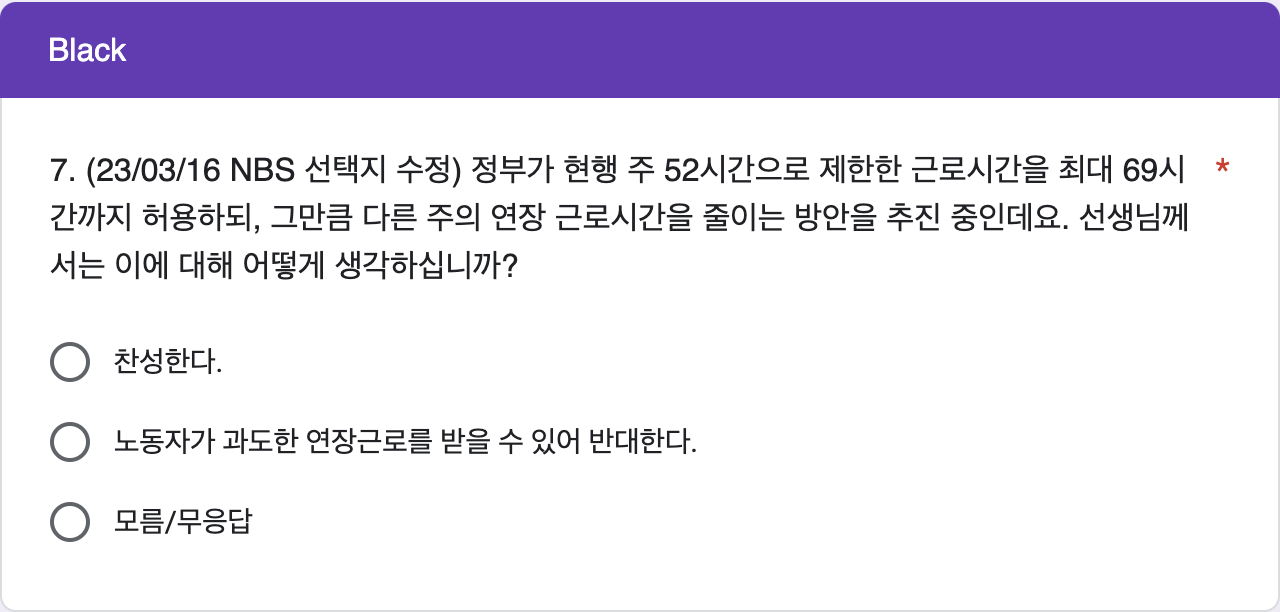
\includegraphics[width=0.67\linewidth]{./pics/Quiz240322_Q7_Black} \end{flushleft}

\subsection{집계}\label{uxc9d1uxacc4-1}

\begin{longtable}[]{@{}
  >{\raggedright\arraybackslash}p{(\linewidth - 8\tabcolsep) * \real{0.4286}}
  >{\centering\arraybackslash}p{(\linewidth - 8\tabcolsep) * \real{0.1558}}
  >{\centering\arraybackslash}p{(\linewidth - 8\tabcolsep) * \real{0.1558}}
  >{\centering\arraybackslash}p{(\linewidth - 8\tabcolsep) * \real{0.1818}}
  >{\centering\arraybackslash}p{(\linewidth - 8\tabcolsep) * \real{0.0779}}@{}}
\toprule\noalign{}
\begin{minipage}[b]{\linewidth}\raggedright
~
\end{minipage} & \begin{minipage}[b]{\linewidth}\centering
찬성한다.
\end{minipage} & \begin{minipage}[b]{\linewidth}\centering
반대한다.
\end{minipage} & \begin{minipage}[b]{\linewidth}\centering
모름/무응답
\end{minipage} & \begin{minipage}[b]{\linewidth}\centering
계
\end{minipage} \\
\midrule\noalign{}
\endhead
\bottomrule\noalign{}
\endlastfoot
\textbf{Red(찬성한다에 부연설명)} & 132 & 78 & 68 & 278 \\
\textbf{Black(반대한다에 부연설명)} & 85 & 146 & 55 & 286 \\
\textbf{계} & 217 & 224 & 123 & 564 \\
\end{longtable}

\begin{longtable}[]{@{}
  >{\raggedleft\arraybackslash}p{(\linewidth - 4\tabcolsep) * \real{0.2361}}
  >{\raggedleft\arraybackslash}p{(\linewidth - 4\tabcolsep) * \real{0.0694}}
  >{\raggedleft\arraybackslash}p{(\linewidth - 4\tabcolsep) * \real{0.2500}}@{}}
\caption{Pearson's Chi-squared test: \texttt{.}}\tabularnewline
\toprule\noalign{}
\begin{minipage}[b]{\linewidth}\raggedleft
Test statistic
\end{minipage} & \begin{minipage}[b]{\linewidth}\raggedleft
df
\end{minipage} & \begin{minipage}[b]{\linewidth}\raggedleft
P value
\end{minipage} \\
\midrule\noalign{}
\endfirsthead
\toprule\noalign{}
\begin{minipage}[b]{\linewidth}\raggedleft
Test statistic
\end{minipage} & \begin{minipage}[b]{\linewidth}\raggedleft
df
\end{minipage} & \begin{minipage}[b]{\linewidth}\raggedleft
P value
\end{minipage} \\
\midrule\noalign{}
\endhead
\bottomrule\noalign{}
\endlastfoot
32.09 & 2 & 1.076e-07 * * * \\
\end{longtable}

Q7의 Red는 주당 근로 69시간제의 도입에 찬반을 묻는 질문 중 찬성을 유도하는 부연설명을 붙였을 때 278명이 응답한 가운데 132명이 ``찬성한다''는 반응을 보이고, 78명이 ``반대한다''는 반응을 보입니다.

Black은 같은 상황에서 반대를 유도하는 부연설명을 붙였을 떄 286명이 응답한 가운데 85명이 ``찬성한다''는 반응을 보이고, 146명이 ``반대한다''는 반응을 보입니다.

그리고 ``모름/무응답''에 답한 인원은 Red에 68명, Black 에 55명이 응답하였습니다.

카이제곱 테스트는 이와 같은 상황에서
찬성을 유도하는 부연설명을 붙인 경우와 반대를 유도하는 부연설명을 붙인 경우에 그 응답의 차이가 통계적으로 유의하다는 것을 보여 줍니다.

카이제곱 통계량은 32.090, 자유도는 2, p-value 는 1.1e-07으로
부연설명을 어디에 붙이느냐에 따라 그 차이가 통계적으로 유의한 것으로 나왔습니다.

여기서 부연설명이 응답에 영향을 끼치지 않는다고 가정해 봅시다.

그렇다면 Red, Black 의 응답은 대부분의 Q1 \textasciitilde{} Q6 에서와 같이 랜덤화 효과에 의하여 통계적으로 유의한 차이를 보이지 않을 것입니다.

그런데 실제로 관찰된 카이제곱 통계값은 통계적으로 유의한 차이를 보여 주고 있습니다.

따라서 부연설명이 영향을 끼치지 않는다는 가정은 티당치 않은 것으로 볼 수밖에 없습니다.

이러한 논증 방식을 귀류법이라 합니다.

\subsection{\% 비교}\label{uxbe44uxad50-2}

\begin{longtable}[]{@{}
  >{\raggedright\arraybackslash}p{(\linewidth - 8\tabcolsep) * \real{0.4177}}
  >{\centering\arraybackslash}p{(\linewidth - 8\tabcolsep) * \real{0.1519}}
  >{\centering\arraybackslash}p{(\linewidth - 8\tabcolsep) * \real{0.1519}}
  >{\centering\arraybackslash}p{(\linewidth - 8\tabcolsep) * \real{0.1772}}
  >{\centering\arraybackslash}p{(\linewidth - 8\tabcolsep) * \real{0.1013}}@{}}
\toprule\noalign{}
\begin{minipage}[b]{\linewidth}\raggedright
~
\end{minipage} & \begin{minipage}[b]{\linewidth}\centering
찬성한다.
\end{minipage} & \begin{minipage}[b]{\linewidth}\centering
반대한다.
\end{minipage} & \begin{minipage}[b]{\linewidth}\centering
모름/무응답
\end{minipage} & \begin{minipage}[b]{\linewidth}\centering
계
\end{minipage} \\
\midrule\noalign{}
\endhead
\bottomrule\noalign{}
\endlastfoot
\textbf{Red(찬성한다에 부연설명)} & 47.5 & 28.1 & 24.5 & 100.0 \\
\textbf{Black(반대한다에 부연설명)} & 29.7 & 51.0 & 19.2 & 100.0 \\
\end{longtable}

찬성을 유도하는 부연설명을 붙인 Red에서 ``찬성한다''고 응답하는사람들의 백분율, 47.5(\%)은 ``반대한다''고 응답하는 사람들의 백분율, 28.1(\%) 보다 높습니다.

반면 반대를 유도하는 부연설명을 붙인 Black에서 ``찬성한다''고 응답하는 사람들의 백분율, 29.7(\%)은 ``반대한다''고 응답하는 사람들의 백분율, 51.0(\%) 보다 훨씬 적습니다.

찬성을 유도하는 부연설명을 붙이느냐, 반대를 유도하는 부연설명을 붙이느냐에 따라 반응이 달라진다는 것을 잘 알 수 있습니다.

Red 와 Black 이 워낙 차이가 나지만 전체적으로 어느 정도가 ``찬성한다''하고 어느 정도가 ``반대한다''고 응답하였는지 합쳐 보겠습니다.

\subsection{\% 합계}\label{uxd569uxacc4-1}

\begin{longtable}[]{@{}
  >{\centering\arraybackslash}p{(\linewidth - 6\tabcolsep) * \real{0.1667}}
  >{\centering\arraybackslash}p{(\linewidth - 6\tabcolsep) * \real{0.1667}}
  >{\centering\arraybackslash}p{(\linewidth - 6\tabcolsep) * \real{0.1944}}
  >{\centering\arraybackslash}p{(\linewidth - 6\tabcolsep) * \real{0.1111}}@{}}
\toprule\noalign{}
\begin{minipage}[b]{\linewidth}\centering
찬성한다.
\end{minipage} & \begin{minipage}[b]{\linewidth}\centering
반대한다.
\end{minipage} & \begin{minipage}[b]{\linewidth}\centering
모름/무응답
\end{minipage} & \begin{minipage}[b]{\linewidth}\centering
계
\end{minipage} \\
\midrule\noalign{}
\endhead
\bottomrule\noalign{}
\endlastfoot
38.5 & 39.7 & 21.8 & 100.0 \\
\end{longtable}

``찬성한다''고 응답한 백분율은 Red, Black 합쳐서 38.5(\%)(으)로 '반대한다''고 응답한 백분율, 39.7(\%) 과 약간 적습니다.

그리고, 모름/무응답이 21.8(\%)로 적지 않습니다.

\subsection{Mosaic Plot}\label{mosaic-plot-6}

\pandocbounded{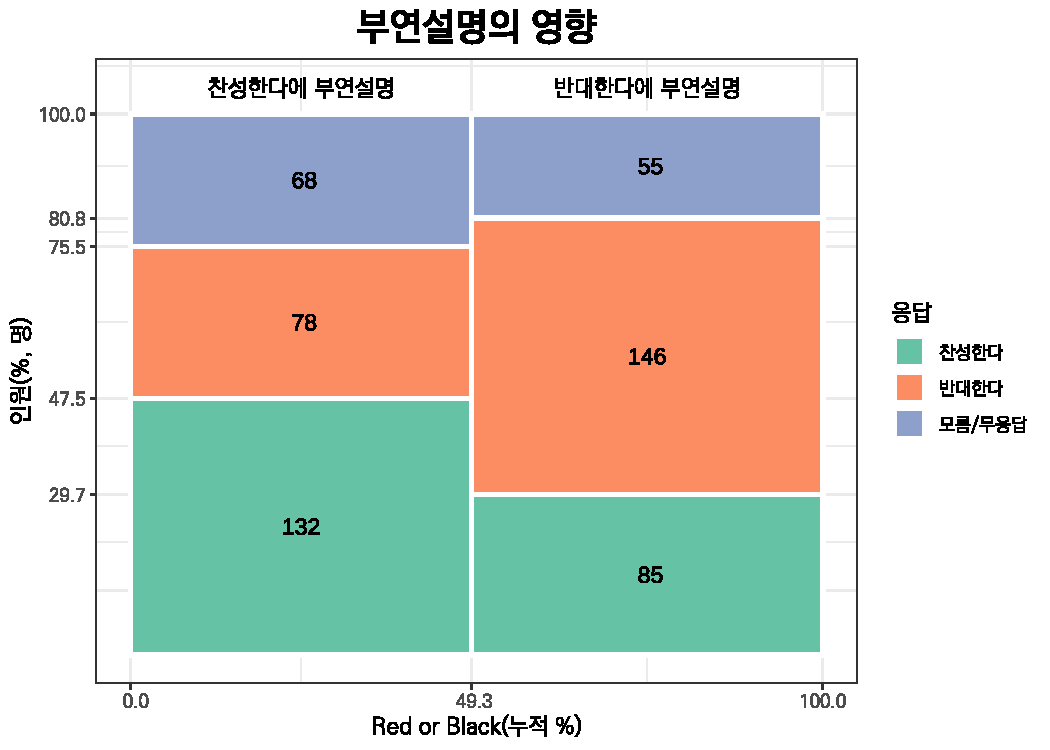
\includegraphics[keepaspectratio]{Quiz_report_2025_files/figure-latex/unnamed-chunk-83-1.pdf}}

Mosaic Plot 은 이 집계결과를 시각적으로 잘 보여줍니다.

찬성을 유도하는 부연설명을 붙인 Red 에서 ``찬성한다''고 응답한 백분율이 높고, 반대를 유도하는 부연설명을 붙인 Black 에서 ``반대한다''고 응답한 백분율이 월등히 높은 것을 시각적으로 알 수 있습니다.

\section{마감 시간으로부터 제출 시간의 분포}\label{uxb9c8uxac10-uxc2dcuxac04uxc73cuxb85cuxbd80uxd130-uxc81cuxcd9c-uxc2dcuxac04uxc758-uxbd84uxd3ec-3}

\subsection{분포표}\label{uxbd84uxd3ecuxd45c-3}

\begin{longtable}[]{@{}
  >{\raggedright\arraybackslash}p{(\linewidth - 30\tabcolsep) * \real{0.1121}}
  >{\centering\arraybackslash}p{(\linewidth - 30\tabcolsep) * \real{0.0654}}
  >{\centering\arraybackslash}p{(\linewidth - 30\tabcolsep) * \real{0.0654}}
  >{\centering\arraybackslash}p{(\linewidth - 30\tabcolsep) * \real{0.0654}}
  >{\centering\arraybackslash}p{(\linewidth - 30\tabcolsep) * \real{0.0654}}
  >{\centering\arraybackslash}p{(\linewidth - 30\tabcolsep) * \real{0.0654}}
  >{\centering\arraybackslash}p{(\linewidth - 30\tabcolsep) * \real{0.0561}}
  >{\centering\arraybackslash}p{(\linewidth - 30\tabcolsep) * \real{0.0561}}
  >{\centering\arraybackslash}p{(\linewidth - 30\tabcolsep) * \real{0.0561}}
  >{\centering\arraybackslash}p{(\linewidth - 30\tabcolsep) * \real{0.0561}}
  >{\centering\arraybackslash}p{(\linewidth - 30\tabcolsep) * \real{0.0561}}
  >{\centering\arraybackslash}p{(\linewidth - 30\tabcolsep) * \real{0.0561}}
  >{\centering\arraybackslash}p{(\linewidth - 30\tabcolsep) * \real{0.0561}}
  >{\centering\arraybackslash}p{(\linewidth - 30\tabcolsep) * \real{0.0561}}
  >{\centering\arraybackslash}p{(\linewidth - 30\tabcolsep) * \real{0.0561}}
  >{\centering\arraybackslash}p{(\linewidth - 30\tabcolsep) * \real{0.0561}}@{}}
\caption{일 단위}\tabularnewline
\toprule\noalign{}
\begin{minipage}[b]{\linewidth}\raggedright
~
\end{minipage} & \begin{minipage}[b]{\linewidth}\centering
14일
\end{minipage} & \begin{minipage}[b]{\linewidth}\centering
13일
\end{minipage} & \begin{minipage}[b]{\linewidth}\centering
12일
\end{minipage} & \begin{minipage}[b]{\linewidth}\centering
11일
\end{minipage} & \begin{minipage}[b]{\linewidth}\centering
10일
\end{minipage} & \begin{minipage}[b]{\linewidth}\centering
9일
\end{minipage} & \begin{minipage}[b]{\linewidth}\centering
8일
\end{minipage} & \begin{minipage}[b]{\linewidth}\centering
7일
\end{minipage} & \begin{minipage}[b]{\linewidth}\centering
6일
\end{minipage} & \begin{minipage}[b]{\linewidth}\centering
5일
\end{minipage} & \begin{minipage}[b]{\linewidth}\centering
4일
\end{minipage} & \begin{minipage}[b]{\linewidth}\centering
3일
\end{minipage} & \begin{minipage}[b]{\linewidth}\centering
2일
\end{minipage} & \begin{minipage}[b]{\linewidth}\centering
1일
\end{minipage} & \begin{minipage}[b]{\linewidth}\centering
계
\end{minipage} \\
\midrule\noalign{}
\endfirsthead
\toprule\noalign{}
\begin{minipage}[b]{\linewidth}\raggedright
~
\end{minipage} & \begin{minipage}[b]{\linewidth}\centering
14일
\end{minipage} & \begin{minipage}[b]{\linewidth}\centering
13일
\end{minipage} & \begin{minipage}[b]{\linewidth}\centering
12일
\end{minipage} & \begin{minipage}[b]{\linewidth}\centering
11일
\end{minipage} & \begin{minipage}[b]{\linewidth}\centering
10일
\end{minipage} & \begin{minipage}[b]{\linewidth}\centering
9일
\end{minipage} & \begin{minipage}[b]{\linewidth}\centering
8일
\end{minipage} & \begin{minipage}[b]{\linewidth}\centering
7일
\end{minipage} & \begin{minipage}[b]{\linewidth}\centering
6일
\end{minipage} & \begin{minipage}[b]{\linewidth}\centering
5일
\end{minipage} & \begin{minipage}[b]{\linewidth}\centering
4일
\end{minipage} & \begin{minipage}[b]{\linewidth}\centering
3일
\end{minipage} & \begin{minipage}[b]{\linewidth}\centering
2일
\end{minipage} & \begin{minipage}[b]{\linewidth}\centering
1일
\end{minipage} & \begin{minipage}[b]{\linewidth}\centering
계
\end{minipage} \\
\midrule\noalign{}
\endhead
\bottomrule\noalign{}
\endlastfoot
\textbf{Red} & 71 & 15 & 13 & 4 & 10 & 3 & 6 & 46 & 20 & 22 & 14 & 20 & 16 & 18 & 278 \\
\textbf{Black} & 71 & 14 & 7 & 7 & 11 & 4 & 6 & 50 & 20 & 14 & 12 & 24 & 17 & 29 & 286 \\
\textbf{계} & 142 & 29 & 20 & 11 & 21 & 7 & 12 & 96 & 40 & 36 & 26 & 44 & 33 & 47 & 564 \\
\end{longtable}

분포표로부터 두 가지 문제를 살펴보겠습니다.

첫째, 날마다 고르게 제출하는가?

둘째, Red, Black 간에 통게적으로 유의한 차이가 있는가?

각 문제를 살펴보기 위해서는 분포표의 일부분을 대상으로 카이제곱 테스트를 수행합니다.

\subsection{날마다 고르게 제출하는가?}\label{uxb0a0uxb9c8uxb2e4-uxace0uxb974uxac8c-uxc81cuxcd9cuxd558uxb294uxac00-3}

\begin{longtable}[]{@{}
  >{\centering\arraybackslash}p{(\linewidth - 26\tabcolsep) * \real{0.0787}}
  >{\centering\arraybackslash}p{(\linewidth - 26\tabcolsep) * \real{0.0787}}
  >{\centering\arraybackslash}p{(\linewidth - 26\tabcolsep) * \real{0.0787}}
  >{\centering\arraybackslash}p{(\linewidth - 26\tabcolsep) * \real{0.0787}}
  >{\centering\arraybackslash}p{(\linewidth - 26\tabcolsep) * \real{0.0787}}
  >{\centering\arraybackslash}p{(\linewidth - 26\tabcolsep) * \real{0.0674}}
  >{\centering\arraybackslash}p{(\linewidth - 26\tabcolsep) * \real{0.0674}}
  >{\centering\arraybackslash}p{(\linewidth - 26\tabcolsep) * \real{0.0674}}
  >{\centering\arraybackslash}p{(\linewidth - 26\tabcolsep) * \real{0.0674}}
  >{\centering\arraybackslash}p{(\linewidth - 26\tabcolsep) * \real{0.0674}}
  >{\centering\arraybackslash}p{(\linewidth - 26\tabcolsep) * \real{0.0674}}
  >{\centering\arraybackslash}p{(\linewidth - 26\tabcolsep) * \real{0.0674}}
  >{\centering\arraybackslash}p{(\linewidth - 26\tabcolsep) * \real{0.0674}}
  >{\centering\arraybackslash}p{(\linewidth - 26\tabcolsep) * \real{0.0674}}@{}}
\toprule\noalign{}
\begin{minipage}[b]{\linewidth}\centering
14일
\end{minipage} & \begin{minipage}[b]{\linewidth}\centering
13일
\end{minipage} & \begin{minipage}[b]{\linewidth}\centering
12일
\end{minipage} & \begin{minipage}[b]{\linewidth}\centering
11일
\end{minipage} & \begin{minipage}[b]{\linewidth}\centering
10일
\end{minipage} & \begin{minipage}[b]{\linewidth}\centering
9일
\end{minipage} & \begin{minipage}[b]{\linewidth}\centering
8일
\end{minipage} & \begin{minipage}[b]{\linewidth}\centering
7일
\end{minipage} & \begin{minipage}[b]{\linewidth}\centering
6일
\end{minipage} & \begin{minipage}[b]{\linewidth}\centering
5일
\end{minipage} & \begin{minipage}[b]{\linewidth}\centering
4일
\end{minipage} & \begin{minipage}[b]{\linewidth}\centering
3일
\end{minipage} & \begin{minipage}[b]{\linewidth}\centering
2일
\end{minipage} & \begin{minipage}[b]{\linewidth}\centering
1일
\end{minipage} \\
\midrule\noalign{}
\endhead
\bottomrule\noalign{}
\endlastfoot
142 & 29 & 20 & 11 & 21 & 7 & 12 & 96 & 40 & 36 & 26 & 44 & 33 & 47 \\
\end{longtable}

\begin{longtable}[]{@{}
  >{\raggedleft\arraybackslash}p{(\linewidth - 4\tabcolsep) * \real{0.2361}}
  >{\raggedleft\arraybackslash}p{(\linewidth - 4\tabcolsep) * \real{0.0694}}
  >{\raggedleft\arraybackslash}p{(\linewidth - 4\tabcolsep) * \real{0.2500}}@{}}
\caption{Chi-squared test for given probabilities: \texttt{.}}\tabularnewline
\toprule\noalign{}
\begin{minipage}[b]{\linewidth}\raggedleft
Test statistic
\end{minipage} & \begin{minipage}[b]{\linewidth}\raggedleft
df
\end{minipage} & \begin{minipage}[b]{\linewidth}\raggedleft
P value
\end{minipage} \\
\midrule\noalign{}
\endfirsthead
\toprule\noalign{}
\begin{minipage}[b]{\linewidth}\raggedleft
Test statistic
\end{minipage} & \begin{minipage}[b]{\linewidth}\raggedleft
df
\end{minipage} & \begin{minipage}[b]{\linewidth}\raggedleft
P value
\end{minipage} \\
\midrule\noalign{}
\endhead
\bottomrule\noalign{}
\endlastfoot
433.4 & 13 & 1.915e-84 * * * \\
\end{longtable}

날마다 고르게 제출하는지 알아 보았습니다.

분포표의 ``계''행에서 '계'열을 제외하고 카이제곱테스트를 수행합니다.

분포표 만으로도 쉽게 파악할 수 있지만 카이제곱테스트가 명확히 해 줍니다.

카이제곱 통계량은 433.43, 자유도는 13.00, p-value 는 1.9e-84 이므로 결코 고르게 제출한다고 말할 수 없습니다.

막대그래프로 살펴 보겠습니다.

\subsection{막대그래프}\label{uxb9c9uxb300uxadf8uxb798uxd504-3}

\pandocbounded{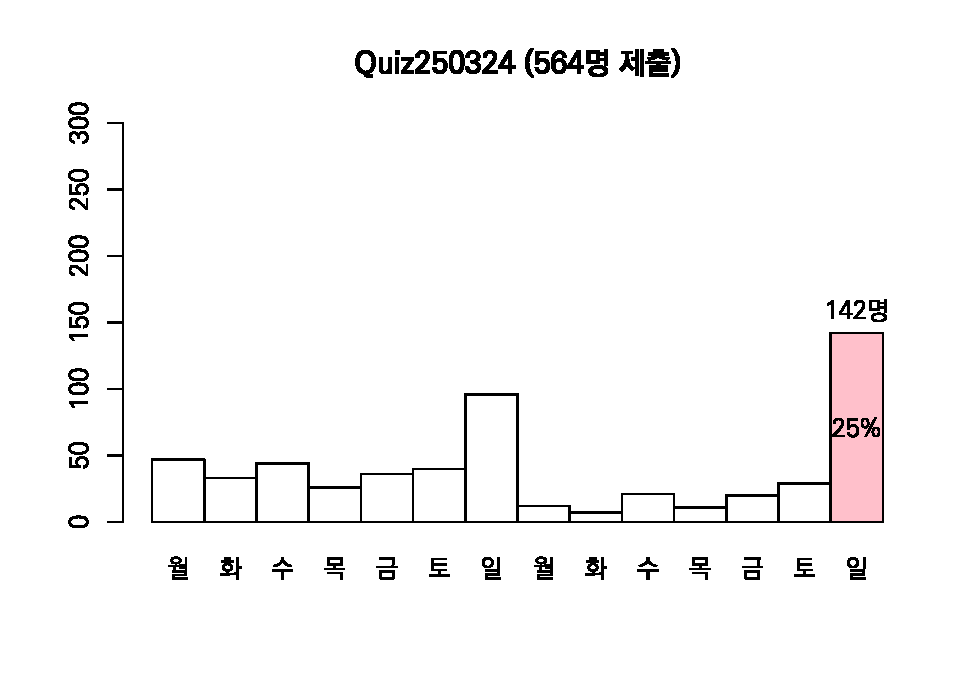
\includegraphics[keepaspectratio]{Quiz_report_2025_files/figure-latex/unnamed-chunk-86-1.pdf}}

막대그래프는 총 제출인원 564(명) 중에 142(명), 25(\%)가 마감일에 몰리는 것을 명확히 보여주고 있습니다.

\subsection{Red, Black 간에 닮았는가?}\label{red-black-uxac04uxc5d0-uxb2eeuxc558uxb294uxac00-3}

\begin{longtable}[]{@{}
  >{\raggedright\arraybackslash}p{(\linewidth - 28\tabcolsep) * \real{0.1188}}
  >{\centering\arraybackslash}p{(\linewidth - 28\tabcolsep) * \real{0.0693}}
  >{\centering\arraybackslash}p{(\linewidth - 28\tabcolsep) * \real{0.0693}}
  >{\centering\arraybackslash}p{(\linewidth - 28\tabcolsep) * \real{0.0693}}
  >{\centering\arraybackslash}p{(\linewidth - 28\tabcolsep) * \real{0.0693}}
  >{\centering\arraybackslash}p{(\linewidth - 28\tabcolsep) * \real{0.0693}}
  >{\centering\arraybackslash}p{(\linewidth - 28\tabcolsep) * \real{0.0594}}
  >{\centering\arraybackslash}p{(\linewidth - 28\tabcolsep) * \real{0.0594}}
  >{\centering\arraybackslash}p{(\linewidth - 28\tabcolsep) * \real{0.0594}}
  >{\centering\arraybackslash}p{(\linewidth - 28\tabcolsep) * \real{0.0594}}
  >{\centering\arraybackslash}p{(\linewidth - 28\tabcolsep) * \real{0.0594}}
  >{\centering\arraybackslash}p{(\linewidth - 28\tabcolsep) * \real{0.0594}}
  >{\centering\arraybackslash}p{(\linewidth - 28\tabcolsep) * \real{0.0594}}
  >{\centering\arraybackslash}p{(\linewidth - 28\tabcolsep) * \real{0.0594}}
  >{\centering\arraybackslash}p{(\linewidth - 28\tabcolsep) * \real{0.0594}}@{}}
\toprule\noalign{}
\begin{minipage}[b]{\linewidth}\raggedright
~
\end{minipage} & \begin{minipage}[b]{\linewidth}\centering
14일
\end{minipage} & \begin{minipage}[b]{\linewidth}\centering
13일
\end{minipage} & \begin{minipage}[b]{\linewidth}\centering
12일
\end{minipage} & \begin{minipage}[b]{\linewidth}\centering
11일
\end{minipage} & \begin{minipage}[b]{\linewidth}\centering
10일
\end{minipage} & \begin{minipage}[b]{\linewidth}\centering
9일
\end{minipage} & \begin{minipage}[b]{\linewidth}\centering
8일
\end{minipage} & \begin{minipage}[b]{\linewidth}\centering
7일
\end{minipage} & \begin{minipage}[b]{\linewidth}\centering
6일
\end{minipage} & \begin{minipage}[b]{\linewidth}\centering
5일
\end{minipage} & \begin{minipage}[b]{\linewidth}\centering
4일
\end{minipage} & \begin{minipage}[b]{\linewidth}\centering
3일
\end{minipage} & \begin{minipage}[b]{\linewidth}\centering
2일
\end{minipage} & \begin{minipage}[b]{\linewidth}\centering
1일
\end{minipage} \\
\midrule\noalign{}
\endhead
\bottomrule\noalign{}
\endlastfoot
\textbf{Red} & 71 & 15 & 13 & 4 & 10 & 3 & 6 & 46 & 20 & 22 & 14 & 20 & 16 & 18 \\
\textbf{Black} & 71 & 14 & 7 & 7 & 11 & 4 & 6 & 50 & 20 & 14 & 12 & 24 & 17 & 29 \\
\end{longtable}

\begin{longtable}[]{@{}
  >{\raggedleft\arraybackslash}p{(\linewidth - 4\tabcolsep) * \real{0.2361}}
  >{\raggedleft\arraybackslash}p{(\linewidth - 4\tabcolsep) * \real{0.0694}}
  >{\raggedleft\arraybackslash}p{(\linewidth - 4\tabcolsep) * \real{0.1389}}@{}}
\caption{Pearson's Chi-squared test: \texttt{.}}\tabularnewline
\toprule\noalign{}
\begin{minipage}[b]{\linewidth}\raggedleft
Test statistic
\end{minipage} & \begin{minipage}[b]{\linewidth}\raggedleft
df
\end{minipage} & \begin{minipage}[b]{\linewidth}\raggedleft
P value
\end{minipage} \\
\midrule\noalign{}
\endfirsthead
\toprule\noalign{}
\begin{minipage}[b]{\linewidth}\raggedleft
Test statistic
\end{minipage} & \begin{minipage}[b]{\linewidth}\raggedleft
df
\end{minipage} & \begin{minipage}[b]{\linewidth}\raggedleft
P value
\end{minipage} \\
\midrule\noalign{}
\endhead
\bottomrule\noalign{}
\endlastfoot
7.798 & 13 & 0.8565 \\
\end{longtable}

제출시간의 분포가 Red, Black 간에 닮았는지 알아 보았습니다.

이번에는 분포표의 첫번째와 두번째 행, '계'열을 제외한 나머지 열에 대해서 카이제곱테스트를 수행합니다.

카이제곱 통계량은 7.798, 자유도는 13, p-value 는 0.8565 이므로 제출 시간의 분포는 Red, Black 간에 통계적으로 유의한 차이가 관찰되지 않습니다.

이 사실을 Mosaic Plot 을 이용하여 시각적으로 살펴보겠습니다.

닮았다고 느껴지나요?

\subsection{Mosaic Plot}\label{mosaic-plot-7}

\pandocbounded{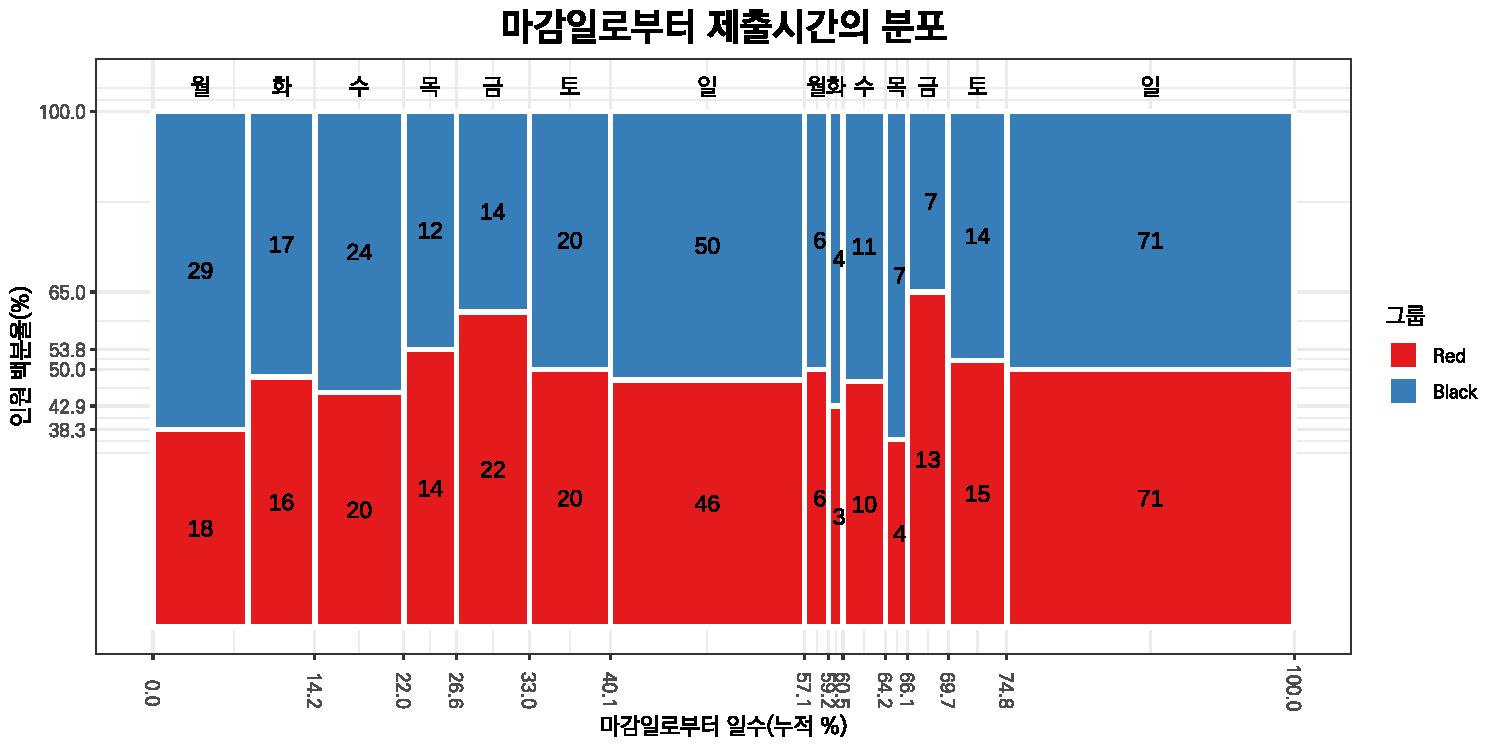
\includegraphics[keepaspectratio]{Quiz_report_2025_files/figure-latex/unnamed-chunk-88-1.pdf}}

\chapter{5주차 데이터 실험 집계}\label{uxc8fcuxcc28-uxb370uxc774uxd130-uxc2e4uxd5d8-uxc9d1uxacc4-4}

\section{실험의 목적}\label{uxc2e4uxd5d8uxc758-uxbaa9uxc801-4}

5주차 구글 예습 설문지 집계결과를 분석합니다.

Q1\textasciitilde Q6에서는 랜덤화의 효과로 Red, Black 이 얼마나 닮았는지 알아봅니다.

Q7에서는 컵에 우유를 반을 쏟은 상황에서 긍정적인 단어를 읽은 그룹하고 부정적인 단어를 읽은 그룹 사이에 어떠한 인식의 차이가 발생하는 지 살펴봅니다.

끝으로 제출시간의 분포가 날마다 고른지, Red, Black 간에는 닮았는지 알아봅니다.

\subsection{Red, Black을 잘못 표시한 사람들}\label{red-blackuxc744-uxc798uxbabb-uxd45cuxc2dcuxd55c-uxc0acuxb78cuxb4e4-4}

\begin{longtable}[]{@{}
  >{\raggedright\arraybackslash}p{(\linewidth - 4\tabcolsep) * \real{0.3611}}
  >{\centering\arraybackslash}p{(\linewidth - 4\tabcolsep) * \real{0.2778}}
  >{\centering\arraybackslash}p{(\linewidth - 4\tabcolsep) * \real{0.3056}}@{}}
\toprule\noalign{}
\begin{minipage}[b]{\linewidth}\raggedright
~
\end{minipage} & \begin{minipage}[b]{\linewidth}\centering
Red(구글예습퀴즈)
\end{minipage} & \begin{minipage}[b]{\linewidth}\centering
Black(구글예습퀴즈)
\end{minipage} \\
\midrule\noalign{}
\endhead
\bottomrule\noalign{}
\endlastfoot
\textbf{Red(랜덤화출석부)} & 274 & 1 \\
\textbf{Black(랜덤화출석부)} & 3 & 280 \\
\textbf{계} & 277 & 281 \\
\end{longtable}

랜덤화출석부에 있는 Red, Black 과 실제 구글설문에 올린 Red, Black 이 다른 사람들의 수효는 4명입니다.

Red를 Black 이라고 한 사람이 1명, Black 을 Red 라고 한 사람이 3명입니다.

두 가지 방법으로 분석합니다.

우선 Red, Black 을 잘못 선택한 4명을 랜덤하게 둘로 나누면 어느 한 쪽 집단에 들어갈 기대인원은 4명을 둘로 나눈 2(명)이고, 표준오차는 4의 제곱근에 1/2을 곱해 준 1명이 됩니다.

실제로 Red를 Black 이라고 한 사람수, 1명이나 Black 을 Red 라고 한 사람수, 3명은 기대인원으로부터 표준오차 범위는 벗어 나지만 표준오차 두 배 범위에는 잘 들어갑니다.

두 번째 분석 방법은 확률을 계산해 보는 것입니다.

Red, Black 을 잘못 선택한 4명을 랜덤하게 둘로 나눌 때, 실제로 관찰된 3명 이상이나 1명이하로 잘못 선택한 사람수가 나올 가능성은 얼마나 되는가 입니다.

이 경우 공평한 동전던지기를 확률 법칙으로 표현한 이항분포로부터 계산할 수 있습니다.

시행횟수가 4이고 한 번 시행에서 성공확률이 1/2 인 이항분포에서 성공횟수가 1이하이거나 3이상을 관찰할 확률은 0.625입니다.

공평한 동전 던지기에서 앞면이 1개 이하 나오는 확률은 3개 이상 나오는 확률과 같기 때문에 사실상 한쪽만 계산해서 2배 해 주면 됩니다.

이 값을 p-value 라고 하는데, p-value가 0.05보다 작을 때 \textbf{통계적으로 유의한 차이를 관찰}하였다고 말합니다.

즉, 공평한 동전을 던지는 것과 같은 과정이라고 가정하였을 때 실제로 관찰된 값들이 가정으로부터 얼마나 떨어져 있는지를 표현한 것입니다.

0.05는 이런 실험을 스무 번 정도 반복하면 1번 나올 정도로 드문 사건을 의미합니다.

즉 가정이 잘못되었다는 것입니다.

그런데 Red, Black 을 잘못 표시한 사람들의 분포에서 관찰된 p-value 는 0.05와는 비교도 안될 정도로 큰 값입니다.

따라서 두 집단이 랜덤화 효과가 작동하여 \textbf{통계적으로 유의한 차이를 보이지 않는다}고 할 수 있습니다.

\subsection{응답인원의 Red, Black}\label{uxc751uxb2f5uxc778uxc6d0uxc758-red-black-4}

Red 로 응답한 인원은 277명, Black 에 응답한 인원은 281명입니다.

전체 응답인원 558 명을 랜덤하게 둘로 나눌 때 어느 한 쪽의 기대인원은 전체 응답인원의 절반인 279명이고, 표준오차는 전체 응답인원의 제곱근에 1/2을 곱해 준 11.8 명입니다.

따라서 Red, Black 각 그룹에 관찰된 인원은 기대인원으로부터 표준오차 범위 안에 들어갑니다.

\section{Q1. 한글의 문자 유형}\label{q1.-uxd55cuxae00uxc758-uxbb38uxc790-uxc720uxd615}

\begin{flushleft}
\includegraphics[width=0.75\linewidth]{./pics/Quiz210323_Q1} \end{flushleft}

\subsection{한글은 민주 문자}\label{uxd55cuxae00uxc740-uxbbfcuxc8fc-uxbb38uxc790}

\begin{longtable}[]{@{}
  >{\raggedright\arraybackslash}p{(\linewidth - 6\tabcolsep) * \real{0.1667}}
  >{\centering\arraybackslash}p{(\linewidth - 6\tabcolsep) * \real{0.1667}}
  >{\centering\arraybackslash}p{(\linewidth - 6\tabcolsep) * \real{0.1944}}
  >{\centering\arraybackslash}p{(\linewidth - 6\tabcolsep) * \real{0.0833}}@{}}
\toprule\noalign{}
\begin{minipage}[b]{\linewidth}\raggedright
~
\end{minipage} & \begin{minipage}[b]{\linewidth}\centering
민주 문자
\end{minipage} & \begin{minipage}[b]{\linewidth}\centering
엘리트 문자
\end{minipage} & \begin{minipage}[b]{\linewidth}\centering
계
\end{minipage} \\
\midrule\noalign{}
\endhead
\bottomrule\noalign{}
\endlastfoot
\textbf{Red} & 261 & 16 & 277 \\
\textbf{Black} & 263 & 18 & 281 \\
\textbf{계} & 524 & 34 & 558 \\
\end{longtable}

\begin{longtable}[]{@{}
  >{\raggedleft\arraybackslash}p{(\linewidth - 4\tabcolsep) * \real{0.2361}}
  >{\raggedleft\arraybackslash}p{(\linewidth - 4\tabcolsep) * \real{0.0694}}
  >{\raggedleft\arraybackslash}p{(\linewidth - 4\tabcolsep) * \real{0.1389}}@{}}
\caption{Pearson's Chi-squared test with Yates' continuity correction: \texttt{.}}\tabularnewline
\toprule\noalign{}
\begin{minipage}[b]{\linewidth}\raggedleft
Test statistic
\end{minipage} & \begin{minipage}[b]{\linewidth}\raggedleft
df
\end{minipage} & \begin{minipage}[b]{\linewidth}\raggedleft
P value
\end{minipage} \\
\midrule\noalign{}
\endfirsthead
\toprule\noalign{}
\begin{minipage}[b]{\linewidth}\raggedleft
Test statistic
\end{minipage} & \begin{minipage}[b]{\linewidth}\raggedleft
df
\end{minipage} & \begin{minipage}[b]{\linewidth}\raggedleft
P value
\end{minipage} \\
\midrule\noalign{}
\endhead
\bottomrule\noalign{}
\endlastfoot
0.01791 & 1 & 0.8935 \\
\end{longtable}

Q1의 집계 결과가 Red, Black 간에 통계적으로 유의한 차이가 있는지 알아보기 위하여 카이제곱 테스트를 수행하였습니다.

그 결과 카이제곱 통계량은 0.018, 자유도는 1 , p-value 는 0.8935이므로 Red, Black 간에 통계적으로 유의한 차이를 보이지 않습니다.

실제로 닮은 게 느껴집니까?

\subsection{한글은 민주 문자(\%)}\label{uxd55cuxae00uxc740-uxbbfcuxc8fc-uxbb38uxc790-1}

\begin{longtable}[]{@{}
  >{\centering\arraybackslash}p{(\linewidth - 4\tabcolsep) * \real{0.1667}}
  >{\centering\arraybackslash}p{(\linewidth - 4\tabcolsep) * \real{0.1944}}
  >{\centering\arraybackslash}p{(\linewidth - 4\tabcolsep) * \real{0.1111}}@{}}
\toprule\noalign{}
\begin{minipage}[b]{\linewidth}\centering
민주 문자
\end{minipage} & \begin{minipage}[b]{\linewidth}\centering
엘리트 문자
\end{minipage} & \begin{minipage}[b]{\linewidth}\centering
계
\end{minipage} \\
\midrule\noalign{}
\endhead
\bottomrule\noalign{}
\endlastfoot
93.9 & 6.1 & 100.0 \\
\end{longtable}

정답률은 Red, Black 을 합하여 계산하는데, 93.9(\%) 입니다.

\section{Q2. 정보혁명과 문자 체계}\label{q2.-uxc815uxbcf4uxd601uxba85uxacfc-uxbb38uxc790-uxccb4uxacc4}

\begin{flushleft}
\includegraphics[width=0.75\linewidth]{./pics/Quiz210323_Q2} \end{flushleft}

\subsection{정보혁명을 이끄는 문자는 한글(집계표)}\label{uxc815uxbcf4uxd601uxba85uxc744-uxc774uxb044uxb294-uxbb38uxc790uxb294-uxd55cuxae00uxc9d1uxacc4uxd45c}

\begin{longtable}[]{@{}
  >{\raggedright\arraybackslash}p{(\linewidth - 6\tabcolsep) * \real{0.1667}}
  >{\centering\arraybackslash}p{(\linewidth - 6\tabcolsep) * \real{0.0972}}
  >{\centering\arraybackslash}p{(\linewidth - 6\tabcolsep) * \real{0.0972}}
  >{\centering\arraybackslash}p{(\linewidth - 6\tabcolsep) * \real{0.0972}}@{}}
\toprule\noalign{}
\begin{minipage}[b]{\linewidth}\raggedright
~
\end{minipage} & \begin{minipage}[b]{\linewidth}\centering
한자
\end{minipage} & \begin{minipage}[b]{\linewidth}\centering
한글
\end{minipage} & \begin{minipage}[b]{\linewidth}\centering
계
\end{minipage} \\
\midrule\noalign{}
\endhead
\bottomrule\noalign{}
\endlastfoot
\textbf{Red} & 23 & 254 & 277 \\
\textbf{Black} & 16 & 265 & 281 \\
\textbf{계} & 39 & 519 & 558 \\
\end{longtable}

\begin{longtable}[]{@{}
  >{\raggedleft\arraybackslash}p{(\linewidth - 4\tabcolsep) * \real{0.2361}}
  >{\raggedleft\arraybackslash}p{(\linewidth - 4\tabcolsep) * \real{0.0694}}
  >{\raggedleft\arraybackslash}p{(\linewidth - 4\tabcolsep) * \real{0.1389}}@{}}
\caption{Pearson's Chi-squared test with Yates' continuity correction: \texttt{.}}\tabularnewline
\toprule\noalign{}
\begin{minipage}[b]{\linewidth}\raggedleft
Test statistic
\end{minipage} & \begin{minipage}[b]{\linewidth}\raggedleft
df
\end{minipage} & \begin{minipage}[b]{\linewidth}\raggedleft
P value
\end{minipage} \\
\midrule\noalign{}
\endfirsthead
\toprule\noalign{}
\begin{minipage}[b]{\linewidth}\raggedleft
Test statistic
\end{minipage} & \begin{minipage}[b]{\linewidth}\raggedleft
df
\end{minipage} & \begin{minipage}[b]{\linewidth}\raggedleft
P value
\end{minipage} \\
\midrule\noalign{}
\endhead
\bottomrule\noalign{}
\endlastfoot
1.087 & 1 & 0.2971 \\
\end{longtable}

Q2의 집계 결과가 Red, Black 간에 통계적으로 유의한 차이가 있는지 알아보기 위하여 카이제곱 테스트를 수행하였습니다.

그 결과 카이제곱 통계량은 1.09, 자유도는 1, p-value 는 0.30이므로 Red, Black 간에 통계적으로 유의한 차이를 보이지 않습니다.

실제로 닮은 게 느껴집니까?

\subsection{정보혁명을 이끄는 문자는 한글(\%)}\label{uxc815uxbcf4uxd601uxba85uxc744-uxc774uxb044uxb294-uxbb38uxc790uxb294-uxd55cuxae00}

\begin{longtable}[]{@{}
  >{\centering\arraybackslash}p{(\linewidth - 4\tabcolsep) * \real{0.0972}}
  >{\centering\arraybackslash}p{(\linewidth - 4\tabcolsep) * \real{0.0972}}
  >{\centering\arraybackslash}p{(\linewidth - 4\tabcolsep) * \real{0.1111}}@{}}
\toprule\noalign{}
\begin{minipage}[b]{\linewidth}\centering
한자
\end{minipage} & \begin{minipage}[b]{\linewidth}\centering
한글
\end{minipage} & \begin{minipage}[b]{\linewidth}\centering
계
\end{minipage} \\
\midrule\noalign{}
\endhead
\bottomrule\noalign{}
\endlastfoot
7.0 & 93.0 & 100.0 \\
\end{longtable}

정답률은 Red, Black 을 합하여 계산하는데, 93.0(\%) 입니다.

\section{Q3. 알기 힘든 전문 용어}\label{q3.-uxc54cuxae30-uxd798uxb4e0-uxc804uxbb38-uxc6a9uxc5b4}

\begin{flushleft}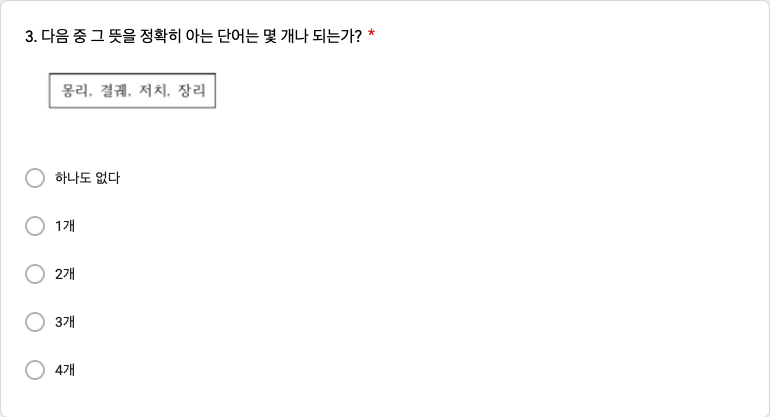
\includegraphics[width=0.75\linewidth]{./pics/Quiz210323_Q3} \end{flushleft}

\subsection{몇 개나 아나요?(집계표)}\label{uxba87-uxac1cuxb098-uxc544uxb098uxc694uxc9d1uxacc4uxd45c}

\begin{longtable}[]{@{}
  >{\raggedright\arraybackslash}p{(\linewidth - 12\tabcolsep) * \real{0.1667}}
  >{\centering\arraybackslash}p{(\linewidth - 12\tabcolsep) * \real{0.1944}}
  >{\centering\arraybackslash}p{(\linewidth - 12\tabcolsep) * \real{0.0833}}
  >{\centering\arraybackslash}p{(\linewidth - 12\tabcolsep) * \real{0.0833}}
  >{\centering\arraybackslash}p{(\linewidth - 12\tabcolsep) * \real{0.0833}}
  >{\centering\arraybackslash}p{(\linewidth - 12\tabcolsep) * \real{0.0833}}
  >{\centering\arraybackslash}p{(\linewidth - 12\tabcolsep) * \real{0.0833}}@{}}
\toprule\noalign{}
\begin{minipage}[b]{\linewidth}\raggedright
~
\end{minipage} & \begin{minipage}[b]{\linewidth}\centering
하나도 없다
\end{minipage} & \begin{minipage}[b]{\linewidth}\centering
1개
\end{minipage} & \begin{minipage}[b]{\linewidth}\centering
2개
\end{minipage} & \begin{minipage}[b]{\linewidth}\centering
3개
\end{minipage} & \begin{minipage}[b]{\linewidth}\centering
4개
\end{minipage} & \begin{minipage}[b]{\linewidth}\centering
계
\end{minipage} \\
\midrule\noalign{}
\endhead
\bottomrule\noalign{}
\endlastfoot
\textbf{Red} & 138 & 72 & 41 & 15 & 11 & 277 \\
\textbf{Black} & 150 & 70 & 40 & 11 & 10 & 281 \\
\textbf{계} & 288 & 142 & 81 & 26 & 21 & 558 \\
\end{longtable}

\begin{longtable}[]{@{}
  >{\raggedleft\arraybackslash}p{(\linewidth - 4\tabcolsep) * \real{0.2361}}
  >{\raggedleft\arraybackslash}p{(\linewidth - 4\tabcolsep) * \real{0.0694}}
  >{\raggedleft\arraybackslash}p{(\linewidth - 4\tabcolsep) * \real{0.1389}}@{}}
\caption{Pearson's Chi-squared test: \texttt{.}}\tabularnewline
\toprule\noalign{}
\begin{minipage}[b]{\linewidth}\raggedleft
Test statistic
\end{minipage} & \begin{minipage}[b]{\linewidth}\raggedleft
df
\end{minipage} & \begin{minipage}[b]{\linewidth}\raggedleft
P value
\end{minipage} \\
\midrule\noalign{}
\endfirsthead
\toprule\noalign{}
\begin{minipage}[b]{\linewidth}\raggedleft
Test statistic
\end{minipage} & \begin{minipage}[b]{\linewidth}\raggedleft
df
\end{minipage} & \begin{minipage}[b]{\linewidth}\raggedleft
P value
\end{minipage} \\
\midrule\noalign{}
\endhead
\bottomrule\noalign{}
\endlastfoot
1.175 & 4 & 0.8822 \\
\end{longtable}

Q3의 집계 결과가 Red, Black 간에 통계적으로 유의한 차이가 있는지 알아보기 위하여 카이제곱 테스트를 수행하였습니다.

그 결과 카이제곱 통계량은 1.175, 자유도는 4, p-value 는 0.8822이므로 Red, Black 간에 통계적으로 유의한 차이를 보이지 않습니다.

실제로 닮은 게 느껴집니까?

\subsection{몇 개나 아나요?(\%)}\label{uxba87-uxac1cuxb098-uxc544uxb098uxc694}

\begin{longtable}[]{@{}
  >{\centering\arraybackslash}p{(\linewidth - 10\tabcolsep) * \real{0.1944}}
  >{\centering\arraybackslash}p{(\linewidth - 10\tabcolsep) * \real{0.0972}}
  >{\centering\arraybackslash}p{(\linewidth - 10\tabcolsep) * \real{0.0972}}
  >{\centering\arraybackslash}p{(\linewidth - 10\tabcolsep) * \real{0.0833}}
  >{\centering\arraybackslash}p{(\linewidth - 10\tabcolsep) * \real{0.0833}}
  >{\centering\arraybackslash}p{(\linewidth - 10\tabcolsep) * \real{0.1111}}@{}}
\toprule\noalign{}
\begin{minipage}[b]{\linewidth}\centering
하나도 없다
\end{minipage} & \begin{minipage}[b]{\linewidth}\centering
1개
\end{minipage} & \begin{minipage}[b]{\linewidth}\centering
2개
\end{minipage} & \begin{minipage}[b]{\linewidth}\centering
3개
\end{minipage} & \begin{minipage}[b]{\linewidth}\centering
4개
\end{minipage} & \begin{minipage}[b]{\linewidth}\centering
계
\end{minipage} \\
\midrule\noalign{}
\endhead
\bottomrule\noalign{}
\endlastfoot
51.6 & 25.4 & 14.5 & 4.7 & 3.8 & 100.0 \\
\end{longtable}

물론, 이 문제에는 정답이 없으므로 정답률은 의미가 없습니다.

가장 많은 비율로 응답한 것이 ``하나도 없다''이고 51.6(\%) 입니다.

\section{Q4. 해방직후 비문해율}\label{q4.-uxd574uxbc29uxc9c1uxd6c4-uxbe44uxbb38uxd574uxc728}

\begin{flushleft}
\includegraphics[width=0.75\linewidth]{./pics/Quiz210323_Q4} \end{flushleft}

\subsection{집계}\label{uxc9d1uxacc4-2}

\begin{longtable}[]{@{}
  >{\raggedright\arraybackslash}p{(\linewidth - 12\tabcolsep) * \real{0.1667}}
  >{\raggedleft\arraybackslash}p{(\linewidth - 12\tabcolsep) * \real{0.0833}}
  >{\raggedleft\arraybackslash}p{(\linewidth - 12\tabcolsep) * \real{0.0833}}
  >{\raggedleft\arraybackslash}p{(\linewidth - 12\tabcolsep) * \real{0.0833}}
  >{\raggedleft\arraybackslash}p{(\linewidth - 12\tabcolsep) * \real{0.0833}}
  >{\raggedleft\arraybackslash}p{(\linewidth - 12\tabcolsep) * \real{0.0833}}
  >{\centering\arraybackslash}p{(\linewidth - 12\tabcolsep) * \real{0.0833}}@{}}
\toprule\noalign{}
\begin{minipage}[b]{\linewidth}\raggedright
~
\end{minipage} & \begin{minipage}[b]{\linewidth}\raggedleft
90\%
\end{minipage} & \begin{minipage}[b]{\linewidth}\raggedleft
80\%
\end{minipage} & \begin{minipage}[b]{\linewidth}\raggedleft
50\%
\end{minipage} & \begin{minipage}[b]{\linewidth}\raggedleft
20\%
\end{minipage} & \begin{minipage}[b]{\linewidth}\raggedleft
10\%
\end{minipage} & \begin{minipage}[b]{\linewidth}\centering
계
\end{minipage} \\
\midrule\noalign{}
\endhead
\bottomrule\noalign{}
\endlastfoot
\textbf{Red} & 13 & 198 & 27 & 28 & 11 & 277 \\
\textbf{Black} & 15 & 193 & 35 & 23 & 15 & 281 \\
\textbf{계} & 28 & 391 & 62 & 51 & 26 & 558 \\
\end{longtable}

\begin{longtable}[]{@{}
  >{\raggedleft\arraybackslash}p{(\linewidth - 4\tabcolsep) * \real{0.2361}}
  >{\raggedleft\arraybackslash}p{(\linewidth - 4\tabcolsep) * \real{0.0694}}
  >{\raggedleft\arraybackslash}p{(\linewidth - 4\tabcolsep) * \real{0.1389}}@{}}
\caption{Pearson's Chi-squared test: \texttt{.}}\tabularnewline
\toprule\noalign{}
\begin{minipage}[b]{\linewidth}\raggedleft
Test statistic
\end{minipage} & \begin{minipage}[b]{\linewidth}\raggedleft
df
\end{minipage} & \begin{minipage}[b]{\linewidth}\raggedleft
P value
\end{minipage} \\
\midrule\noalign{}
\endfirsthead
\toprule\noalign{}
\begin{minipage}[b]{\linewidth}\raggedleft
Test statistic
\end{minipage} & \begin{minipage}[b]{\linewidth}\raggedleft
df
\end{minipage} & \begin{minipage}[b]{\linewidth}\raggedleft
P value
\end{minipage} \\
\midrule\noalign{}
\endhead
\bottomrule\noalign{}
\endlastfoot
2.316 & 4 & 0.6778 \\
\end{longtable}

Q4의 집계 결과가 Red, Black 간에 통계적으로 유의한 차이가 있는지 알아보기 위하여 카이제곱 테스트를 수행하였습니다.

그 결과 카이제곱 통계량은 2.316, 자유도는 4, p-value 는 0.6778이므로 Red, Black 간에 통계적으로 유의한 차이를 보이지 않습니다.

실제로 닮은 게 느껴집니까?

\subsection{\%}\label{section}

\begin{longtable}[]{@{}
  >{\raggedleft\arraybackslash}p{(\linewidth - 10\tabcolsep) * \real{0.0833}}
  >{\raggedleft\arraybackslash}p{(\linewidth - 10\tabcolsep) * \real{0.0972}}
  >{\raggedleft\arraybackslash}p{(\linewidth - 10\tabcolsep) * \real{0.0972}}
  >{\raggedleft\arraybackslash}p{(\linewidth - 10\tabcolsep) * \real{0.0833}}
  >{\raggedleft\arraybackslash}p{(\linewidth - 10\tabcolsep) * \real{0.0833}}
  >{\centering\arraybackslash}p{(\linewidth - 10\tabcolsep) * \real{0.1111}}@{}}
\toprule\noalign{}
\begin{minipage}[b]{\linewidth}\raggedleft
90\%
\end{minipage} & \begin{minipage}[b]{\linewidth}\raggedleft
80\%
\end{minipage} & \begin{minipage}[b]{\linewidth}\raggedleft
50\%
\end{minipage} & \begin{minipage}[b]{\linewidth}\raggedleft
20\%
\end{minipage} & \begin{minipage}[b]{\linewidth}\raggedleft
10\%
\end{minipage} & \begin{minipage}[b]{\linewidth}\centering
계
\end{minipage} \\
\midrule\noalign{}
\endhead
\bottomrule\noalign{}
\endlastfoot
5.0 & 70.1 & 11.1 & 9.1 & 4.7 & 100.0 \\
\end{longtable}

정답률은 Red, Black 을 합하여 계산하는데, 70.1(\%) 입니다.

\section{Q5. 세대간 문해력 격차}\label{q5.-uxc138uxb300uxac04-uxbb38uxd574uxb825-uxaca9uxcc28}

\begin{flushleft}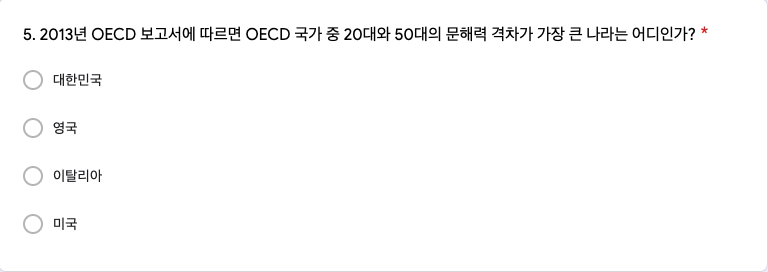
\includegraphics[width=0.75\linewidth]{./pics/Quiz210323_Q5} \end{flushleft}

\subsection{집계}\label{uxc9d1uxacc4-3}

\begin{longtable}[]{@{}
  >{\raggedright\arraybackslash}p{(\linewidth - 10\tabcolsep) * \real{0.1667}}
  >{\centering\arraybackslash}p{(\linewidth - 10\tabcolsep) * \real{0.1528}}
  >{\centering\arraybackslash}p{(\linewidth - 10\tabcolsep) * \real{0.0972}}
  >{\centering\arraybackslash}p{(\linewidth - 10\tabcolsep) * \real{0.1528}}
  >{\centering\arraybackslash}p{(\linewidth - 10\tabcolsep) * \real{0.0972}}
  >{\centering\arraybackslash}p{(\linewidth - 10\tabcolsep) * \real{0.0972}}@{}}
\toprule\noalign{}
\begin{minipage}[b]{\linewidth}\raggedright
~
\end{minipage} & \begin{minipage}[b]{\linewidth}\centering
대한민국
\end{minipage} & \begin{minipage}[b]{\linewidth}\centering
영국
\end{minipage} & \begin{minipage}[b]{\linewidth}\centering
이탈리아
\end{minipage} & \begin{minipage}[b]{\linewidth}\centering
미국
\end{minipage} & \begin{minipage}[b]{\linewidth}\centering
계
\end{minipage} \\
\midrule\noalign{}
\endhead
\bottomrule\noalign{}
\endlastfoot
\textbf{Red} & 212 & 18 & 18 & 29 & 277 \\
\textbf{Black} & 219 & 14 & 15 & 33 & 281 \\
\textbf{계} & 431 & 32 & 33 & 62 & 558 \\
\end{longtable}

\begin{longtable}[]{@{}
  >{\raggedleft\arraybackslash}p{(\linewidth - 4\tabcolsep) * \real{0.2361}}
  >{\raggedleft\arraybackslash}p{(\linewidth - 4\tabcolsep) * \real{0.0694}}
  >{\raggedleft\arraybackslash}p{(\linewidth - 4\tabcolsep) * \real{0.1389}}@{}}
\caption{Pearson's Chi-squared test: \texttt{.}}\tabularnewline
\toprule\noalign{}
\begin{minipage}[b]{\linewidth}\raggedleft
Test statistic
\end{minipage} & \begin{minipage}[b]{\linewidth}\raggedleft
df
\end{minipage} & \begin{minipage}[b]{\linewidth}\raggedleft
P value
\end{minipage} \\
\midrule\noalign{}
\endfirsthead
\toprule\noalign{}
\begin{minipage}[b]{\linewidth}\raggedleft
Test statistic
\end{minipage} & \begin{minipage}[b]{\linewidth}\raggedleft
df
\end{minipage} & \begin{minipage}[b]{\linewidth}\raggedleft
P value
\end{minipage} \\
\midrule\noalign{}
\endhead
\bottomrule\noalign{}
\endlastfoot
1.116 & 3 & 0.7732 \\
\end{longtable}

Q5의 집계 결과가 Red, Black 간에 통계적으로 유의한 차이가 있는지 알아보기 위하여 카이제곱 테스트를 수행하였습니다.

그 결과 카이제곱 통계량은 1.116, 자유도는 3, p-value 는 0.7732이므로 Red, Black 간에 통계적으로 유의한 차이를 보이지 않습니다.

실제로 닮은 게 느껴집니까?

\subsection{\%}\label{section-1}

\begin{longtable}[]{@{}
  >{\centering\arraybackslash}p{(\linewidth - 8\tabcolsep) * \real{0.1528}}
  >{\centering\arraybackslash}p{(\linewidth - 8\tabcolsep) * \real{0.0972}}
  >{\centering\arraybackslash}p{(\linewidth - 8\tabcolsep) * \real{0.1528}}
  >{\centering\arraybackslash}p{(\linewidth - 8\tabcolsep) * \real{0.0972}}
  >{\centering\arraybackslash}p{(\linewidth - 8\tabcolsep) * \real{0.1111}}@{}}
\toprule\noalign{}
\begin{minipage}[b]{\linewidth}\centering
대한민국
\end{minipage} & \begin{minipage}[b]{\linewidth}\centering
영국
\end{minipage} & \begin{minipage}[b]{\linewidth}\centering
이탈리아
\end{minipage} & \begin{minipage}[b]{\linewidth}\centering
미국
\end{minipage} & \begin{minipage}[b]{\linewidth}\centering
계
\end{minipage} \\
\midrule\noalign{}
\endhead
\bottomrule\noalign{}
\endlastfoot
77.2 & 5.7 & 5.9 & 11.1 & 100.0 \\
\end{longtable}

정답률은 Red, Black 을 합하여 계산하는데, 77.2(\%) 입니다.

\section{Q6. 문해력 격차의 파급효과}\label{q6.-uxbb38uxd574uxb825-uxaca9uxcc28uxc758-uxd30cuxae09uxd6a8uxacfc}

\begin{flushleft}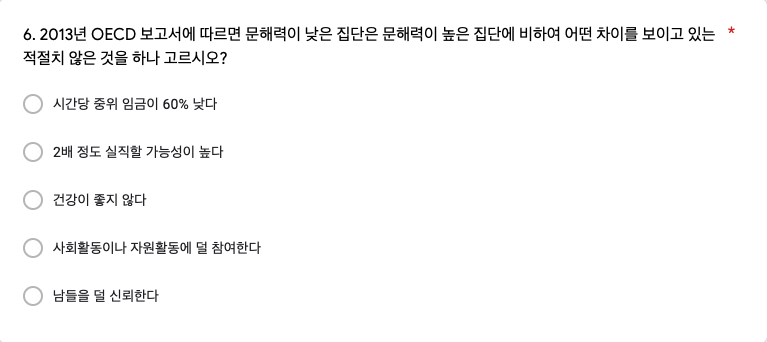
\includegraphics[width=0.75\linewidth]{./pics/Quiz210323_Q6} \end{flushleft}

\subsection{집계}\label{uxc9d1uxacc4-4}

\begin{longtable}[]{@{}
  >{\raggedright\arraybackslash}p{(\linewidth - 12\tabcolsep) * \real{0.1463}}
  >{\centering\arraybackslash}p{(\linewidth - 12\tabcolsep) * \real{0.1951}}
  >{\centering\arraybackslash}p{(\linewidth - 12\tabcolsep) * \real{0.1707}}
  >{\centering\arraybackslash}p{(\linewidth - 12\tabcolsep) * \real{0.1463}}
  >{\centering\arraybackslash}p{(\linewidth - 12\tabcolsep) * \real{0.1463}}
  >{\centering\arraybackslash}p{(\linewidth - 12\tabcolsep) * \real{0.1220}}
  >{\centering\arraybackslash}p{(\linewidth - 12\tabcolsep) * \real{0.0732}}@{}}
\toprule\noalign{}
\begin{minipage}[b]{\linewidth}\raggedright
~
\end{minipage} & \begin{minipage}[b]{\linewidth}\centering
60\% 낮은 임금
\end{minipage} & \begin{minipage}[b]{\linewidth}\centering
실직 가능성
\end{minipage} & \begin{minipage}[b]{\linewidth}\centering
나쁜 건강
\end{minipage} & \begin{minipage}[b]{\linewidth}\centering
활동 불참
\end{minipage} & \begin{minipage}[b]{\linewidth}\centering
덜 신뢰
\end{minipage} & \begin{minipage}[b]{\linewidth}\centering
계
\end{minipage} \\
\midrule\noalign{}
\endhead
\bottomrule\noalign{}
\endlastfoot
\textbf{Red} & 153 & 24 & 40 & 23 & 37 & 277 \\
\textbf{Black} & 152 & 20 & 39 & 20 & 50 & 281 \\
\textbf{계} & 305 & 44 & 79 & 43 & 87 & 558 \\
\end{longtable}

\begin{longtable}[]{@{}
  >{\raggedleft\arraybackslash}p{(\linewidth - 4\tabcolsep) * \real{0.2361}}
  >{\raggedleft\arraybackslash}p{(\linewidth - 4\tabcolsep) * \real{0.0694}}
  >{\raggedleft\arraybackslash}p{(\linewidth - 4\tabcolsep) * \real{0.1389}}@{}}
\caption{Pearson's Chi-squared test: \texttt{.}}\tabularnewline
\toprule\noalign{}
\begin{minipage}[b]{\linewidth}\raggedleft
Test statistic
\end{minipage} & \begin{minipage}[b]{\linewidth}\raggedleft
df
\end{minipage} & \begin{minipage}[b]{\linewidth}\raggedleft
P value
\end{minipage} \\
\midrule\noalign{}
\endfirsthead
\toprule\noalign{}
\begin{minipage}[b]{\linewidth}\raggedleft
Test statistic
\end{minipage} & \begin{minipage}[b]{\linewidth}\raggedleft
df
\end{minipage} & \begin{minipage}[b]{\linewidth}\raggedleft
P value
\end{minipage} \\
\midrule\noalign{}
\endhead
\bottomrule\noalign{}
\endlastfoot
2.503 & 4 & 0.6441 \\
\end{longtable}

Q6의 집계 결과가 Red, Black 간에 통계적으로 유의한 차이가 있는지 알아보기 위하여 카이제곱 테스트를 수행하였습니다.

그 결과 카이제곱 통계량은 2.503, 자유도는 4, p-value 는 0.6441이므로 Red, Black 간에 통계적으로 유의한 차이를 보이지 않습니다.

실제로 닮은 게 느껴집니까?

\subsection{\%}\label{section-2}

\begin{longtable}[]{@{}
  >{\centering\arraybackslash}p{(\linewidth - 10\tabcolsep) * \real{0.2162}}
  >{\centering\arraybackslash}p{(\linewidth - 10\tabcolsep) * \real{0.1892}}
  >{\centering\arraybackslash}p{(\linewidth - 10\tabcolsep) * \real{0.1622}}
  >{\centering\arraybackslash}p{(\linewidth - 10\tabcolsep) * \real{0.1622}}
  >{\centering\arraybackslash}p{(\linewidth - 10\tabcolsep) * \real{0.1351}}
  >{\centering\arraybackslash}p{(\linewidth - 10\tabcolsep) * \real{0.1351}}@{}}
\toprule\noalign{}
\begin{minipage}[b]{\linewidth}\centering
60\% 낮은 임금
\end{minipage} & \begin{minipage}[b]{\linewidth}\centering
실직 가능성
\end{minipage} & \begin{minipage}[b]{\linewidth}\centering
나쁜 건강
\end{minipage} & \begin{minipage}[b]{\linewidth}\centering
활동 불참
\end{minipage} & \begin{minipage}[b]{\linewidth}\centering
덜 신뢰
\end{minipage} & \begin{minipage}[b]{\linewidth}\centering
계
\end{minipage} \\
\midrule\noalign{}
\endhead
\bottomrule\noalign{}
\endlastfoot
54.7 & 7.9 & 14.2 & 7.7 & 15.6 & 100.0 \\
\end{longtable}

정답률은 Red, Black 을 합하여 계산하는데, 54.7(\%) 입니다.

\section{Q7. 프레임을 설정하는 단어의 힘}\label{q7.-uxd504uxb808uxc784uxc744-uxc124uxc815uxd558uxb294-uxb2e8uxc5b4uxc758-uxd798}

컵 가득 음료수를 채웠는데 미끄러지면서 반을 쏟았습니다.

이 상황에서 어떤 사람은 ``그래도 반이 남았네''라고 긍정적 반응을 하고 또 다른 사람은 ``어쩌나 반 밖에 안 남았네''라고 부정적 반응을 보일 수 있습니다.

만약, 반응을 보이기 전에 Red 에는 긍정적 단어들을 읽게 하고, Black 에는 부정적 단어들을 읽게 한 후 반응을 물어보면 어떻게 될까요?

Red, Black 의 성격상 단어를 보기 전에는 긍정적 반응의 비율과 부정적 반응의 비율이 닮을 것으로 기대됩니다.

그러나 단어를 보고 나서는 반응이 극명하게 나뉘는 것을 관찰하게 됩니다.

통계적으로 매우, 매우, \ldots{} 유의한 차이를 보여 줍니다.

이것도 일종의 프레이밍이 인식에 미치는 영향이라고 할 수 있겠습니다.

힘든 상황이라도 긍정적인 생각을 가져야겠죠?

\begin{flushleft}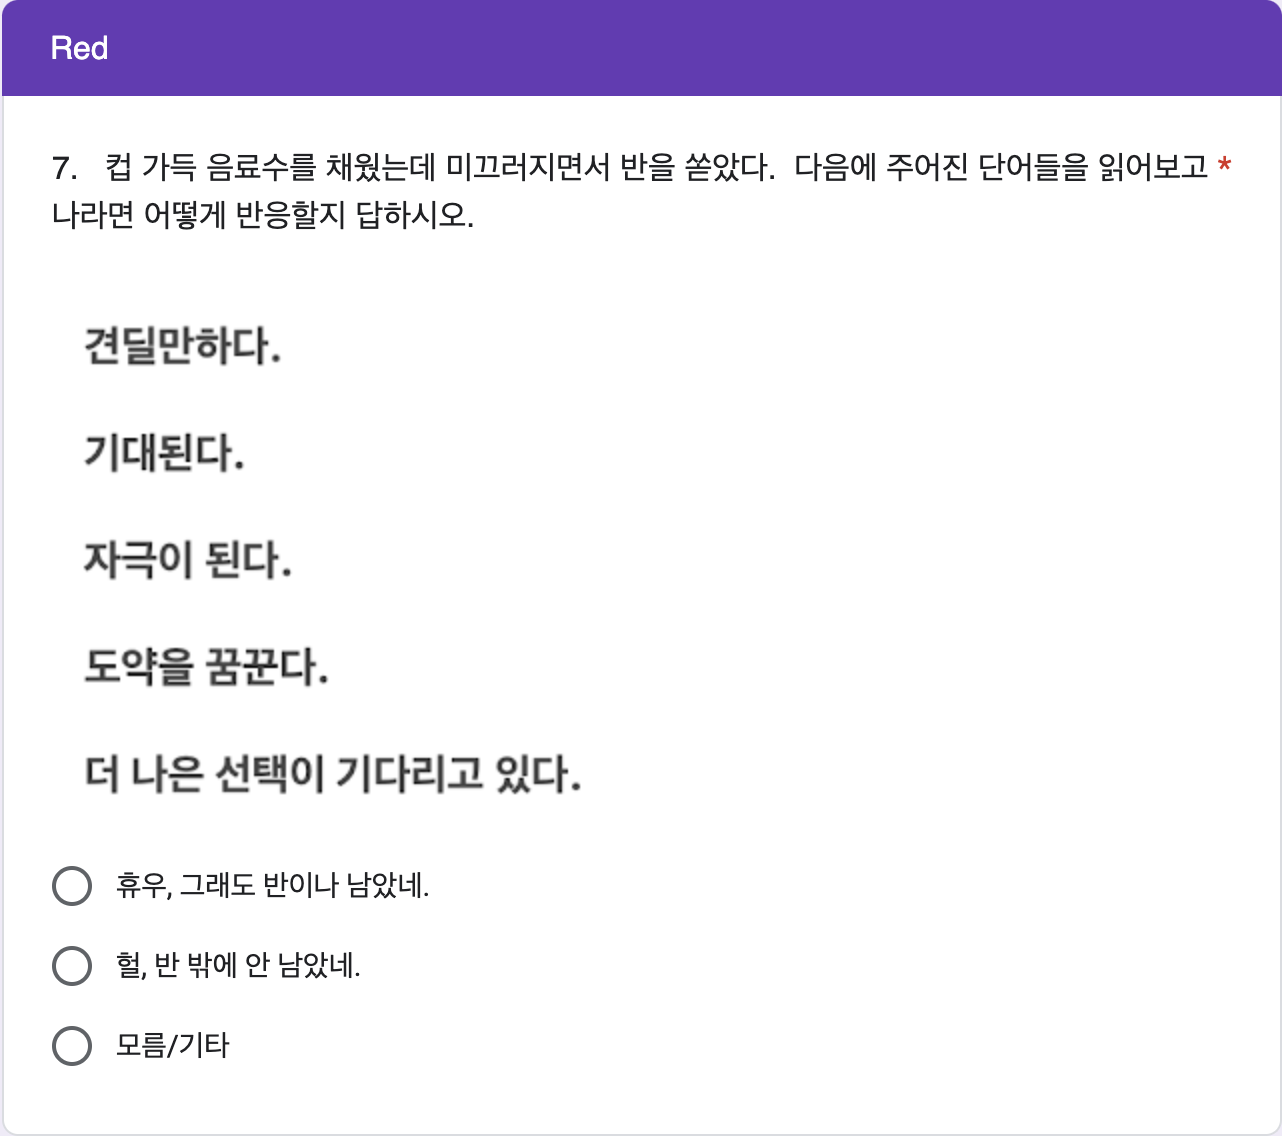
\includegraphics[width=0.67\linewidth]{./pics/Quiz240329_Q7_Red} \end{flushleft}

\begin{flushleft}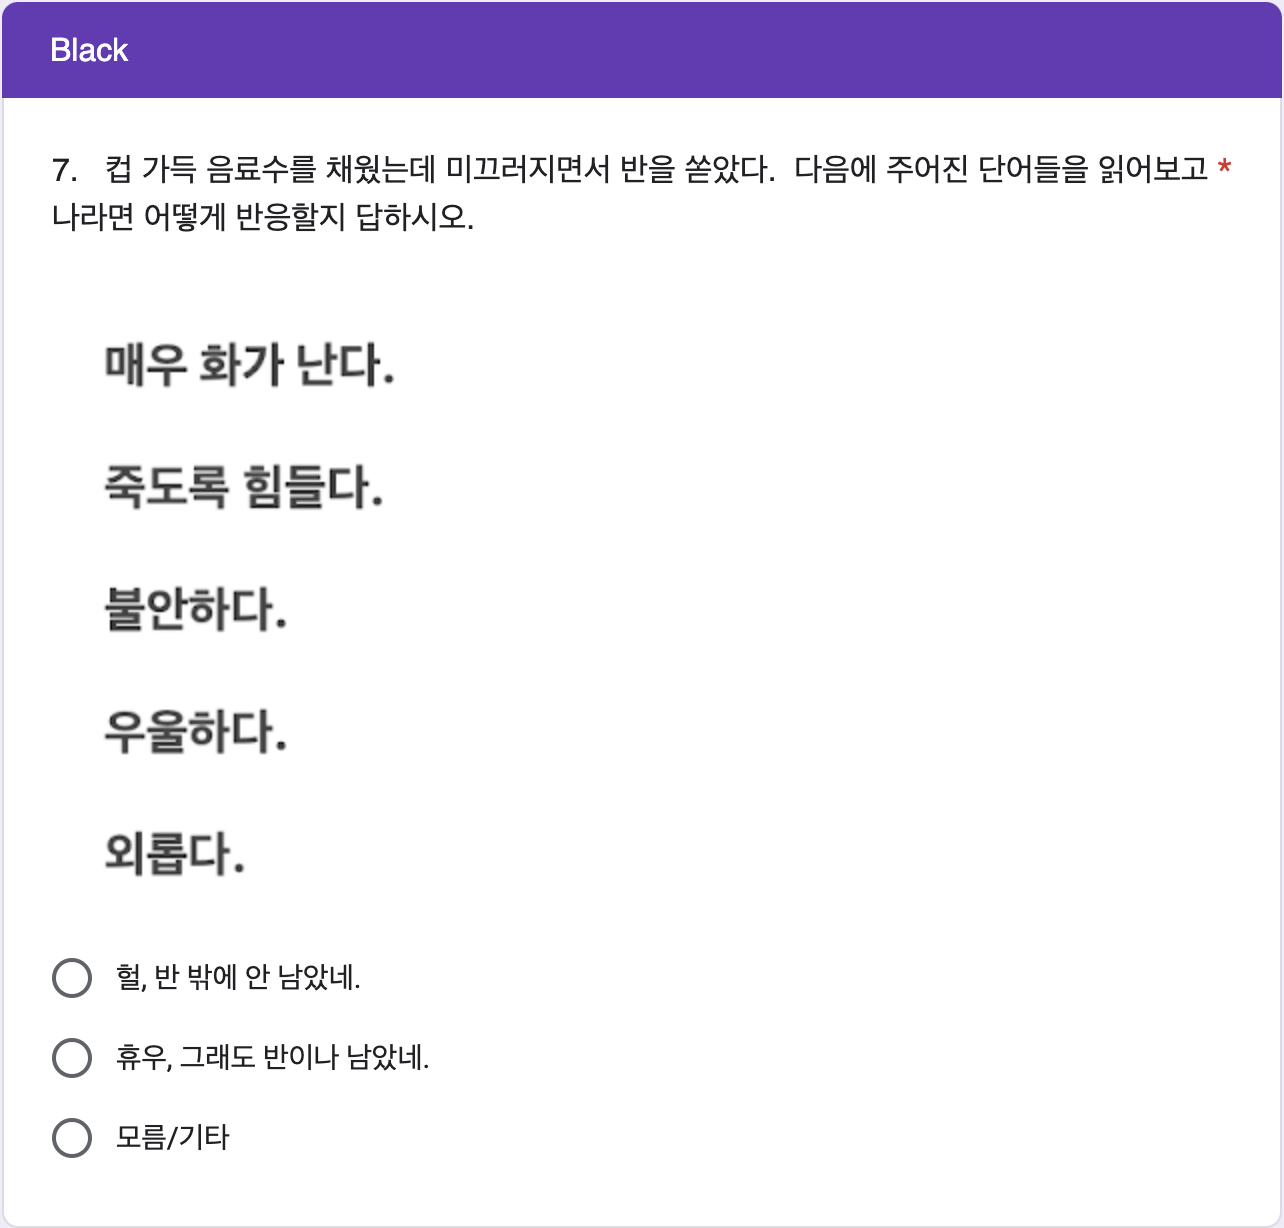
\includegraphics[width=0.67\linewidth]{./pics/Quiz240329_Q7_Black} \end{flushleft}

\subsection{집계}\label{uxc9d1uxacc4-5}

\begin{longtable}[]{@{}
  >{\raggedright\arraybackslash}p{(\linewidth - 8\tabcolsep) * \real{0.3472}}
  >{\centering\arraybackslash}p{(\linewidth - 8\tabcolsep) * \real{0.1250}}
  >{\centering\arraybackslash}p{(\linewidth - 8\tabcolsep) * \real{0.1250}}
  >{\centering\arraybackslash}p{(\linewidth - 8\tabcolsep) * \real{0.1667}}
  >{\centering\arraybackslash}p{(\linewidth - 8\tabcolsep) * \real{0.0833}}@{}}
\toprule\noalign{}
\begin{minipage}[b]{\linewidth}\raggedright
~
\end{minipage} & \begin{minipage}[b]{\linewidth}\centering
반이나
\end{minipage} & \begin{minipage}[b]{\linewidth}\centering
반밖에
\end{minipage} & \begin{minipage}[b]{\linewidth}\centering
모름/기타
\end{minipage} & \begin{minipage}[b]{\linewidth}\centering
계
\end{minipage} \\
\midrule\noalign{}
\endhead
\bottomrule\noalign{}
\endlastfoot
\textbf{Red(긍정적 단어)} & 213 & 49 & 15 & 277 \\
\textbf{Black(부정적 단어)} & 83 & 183 & 15 & 281 \\
\textbf{계} & 296 & 232 & 30 & 558 \\
\end{longtable}

\begin{longtable}[]{@{}
  >{\raggedleft\arraybackslash}p{(\linewidth - 4\tabcolsep) * \real{0.2361}}
  >{\raggedleft\arraybackslash}p{(\linewidth - 4\tabcolsep) * \real{0.0694}}
  >{\raggedleft\arraybackslash}p{(\linewidth - 4\tabcolsep) * \real{0.2500}}@{}}
\caption{Pearson's Chi-squared test: \texttt{.}}\tabularnewline
\toprule\noalign{}
\begin{minipage}[b]{\linewidth}\raggedleft
Test statistic
\end{minipage} & \begin{minipage}[b]{\linewidth}\raggedleft
df
\end{minipage} & \begin{minipage}[b]{\linewidth}\raggedleft
P value
\end{minipage} \\
\midrule\noalign{}
\endfirsthead
\toprule\noalign{}
\begin{minipage}[b]{\linewidth}\raggedleft
Test statistic
\end{minipage} & \begin{minipage}[b]{\linewidth}\raggedleft
df
\end{minipage} & \begin{minipage}[b]{\linewidth}\raggedleft
P value
\end{minipage} \\
\midrule\noalign{}
\endhead
\bottomrule\noalign{}
\endlastfoot
134.5 & 2 & 6.315e-30 * * * \\
\end{longtable}

Q7의 Red는 음료수를 쏟은 상황에서 ``견딜만 하다'' 등의 긍정적인 단어들을 본 사람들인 데 277명이 응답한 가운데 213명이 ``반이나'' 남아 있다는 반응을 보이고, 49명이 ``반 밖에'' 안 남았다는 반응을 보입니다.

Black은 같은 상황에서 ``매우 화가 난다'' 등의 부정적인 단어들을 본 사람들인 데 281명이 응답한 가운데 83명이 ``반이나'' 남아 있다는 반응을 보이고, 183명이 ``반 밖에'' 안 남았다는 반응을 보입니다.

그리고 ``모름/기타''에 답한 인원은 Red에 15명, Black 에 15명이었습니다.

랜덤화 효과일까요?

``모름/기타''의 응답이 유난히 닮은 게 이런 해석을 불러 일으킵니다.

카이제곱 테스트는 이와 같은 상황에서 단어들을 이용하여 긍정적인 프레임을 구성한 경우와 부정적인 프레임을 구성한 경우에 그 차이가 통계적으로 매우, 매우, \ldots{} 유의하다는 것을 보여 줍니다.

카이제곱 통계량은 134.469, 자유도는 2, p-value 는 6.3e-30
긍정적인 단어나 부정적인 단어를 단지 읽는 것만으로도 프레임이 설정되어 반응이 다르게 나온다는 것을 보여줍니다.

여기서 긍정이나 부정 프레이밍이 응답에 영향을 끼치지 않는다고 가정해 봅시다.

그렇다면 Red, Black 의 응답은 Q1 \textasciitilde{} Q6에서와 같이 랜덤화 효과에 의하여 통계적으로 유의한 차이를 보이지 않을 것입니다.

그런데 실제로 관찰된 카이제곱 통계값은 통계적으로 매우 유의한 차이를 보여 줍니다.

따라서 긍정이나 부정 프레이밍이 영향을 끼치지 않는다는 가정이 잘못되었다는 것을 논리적으로 입증할 수 있습니다.

이러한 논증 방식을 귀류법이라 합니다.

\subsection{\% 비교.}\label{uxbe44uxad50.-1}

\begin{longtable}[]{@{}
  >{\raggedright\arraybackslash}p{(\linewidth - 8\tabcolsep) * \real{0.3472}}
  >{\centering\arraybackslash}p{(\linewidth - 8\tabcolsep) * \real{0.1250}}
  >{\centering\arraybackslash}p{(\linewidth - 8\tabcolsep) * \real{0.1250}}
  >{\centering\arraybackslash}p{(\linewidth - 8\tabcolsep) * \real{0.1667}}
  >{\centering\arraybackslash}p{(\linewidth - 8\tabcolsep) * \real{0.1111}}@{}}
\toprule\noalign{}
\begin{minipage}[b]{\linewidth}\raggedright
~
\end{minipage} & \begin{minipage}[b]{\linewidth}\centering
반이나
\end{minipage} & \begin{minipage}[b]{\linewidth}\centering
반밖에
\end{minipage} & \begin{minipage}[b]{\linewidth}\centering
모름/기타
\end{minipage} & \begin{minipage}[b]{\linewidth}\centering
계
\end{minipage} \\
\midrule\noalign{}
\endhead
\bottomrule\noalign{}
\endlastfoot
\textbf{Red(긍정적 단어)} & 76.9 & 17.7 & 5.4 & 100.0 \\
\textbf{Black(부정적 단어)} & 29.5 & 65.1 & 5.3 & 100.0 \\
\end{longtable}

긍정적인 단어들을 읽어 본 Red에서 ``반이나'' 남았다고 응답하는사람들의 백분율, 76.9(\%)은 ``반 밖에'' 안 남았다고 응답하는 사람들의 백분율, 17.7(\%) 보다 월등히 높습니다.

반면 부정적인 단어들을 읽어 본 Black에서 ``반이나'' 남았다고 응답하는사람들의 백분율, 29.5(\%)은 ``반 밖에'' 안 남았다고 응답하는 사람들의 백분율, 65.1(\%) 보다 훨씬 적습니다.

긍정적인 단어를 읽느냐, 부정적인 단어를 읽느냐에 따라 형성된 프레임의 영향이 막대하다는 것을 잘 알 수 있습니다.

Red 와 Black 이 워낙 차이가 나지만 전체적으로 어느 정도가 ``반이나'' 남았다, 혹은 ``반 밖에'' 안 남았다고 응답하였는지 합쳐 보겠습니다.

\subsection{\% 합산}\label{uxd569uxc0b0}

\begin{longtable}[]{@{}
  >{\centering\arraybackslash}p{(\linewidth - 6\tabcolsep) * \real{0.1250}}
  >{\centering\arraybackslash}p{(\linewidth - 6\tabcolsep) * \real{0.1250}}
  >{\centering\arraybackslash}p{(\linewidth - 6\tabcolsep) * \real{0.1667}}
  >{\centering\arraybackslash}p{(\linewidth - 6\tabcolsep) * \real{0.1111}}@{}}
\toprule\noalign{}
\begin{minipage}[b]{\linewidth}\centering
반이나
\end{minipage} & \begin{minipage}[b]{\linewidth}\centering
반밖에
\end{minipage} & \begin{minipage}[b]{\linewidth}\centering
모름/기타
\end{minipage} & \begin{minipage}[b]{\linewidth}\centering
계
\end{minipage} \\
\midrule\noalign{}
\endhead
\bottomrule\noalign{}
\endlastfoot
53.0 & 41.6 & 5.4 & 100.0 \\
\end{longtable}

``반이나'' 남아 있다고 응답한 백분율은 Red, Black 합쳐서 53.0(\%)(으)로 '반 밖에 '' 안 남아 있다고 응답한 백분율, 41.6(\%) 보다 상당히 많습니다.

\subsection{Mosaic Plot}\label{mosaic-plot-8}

\pandocbounded{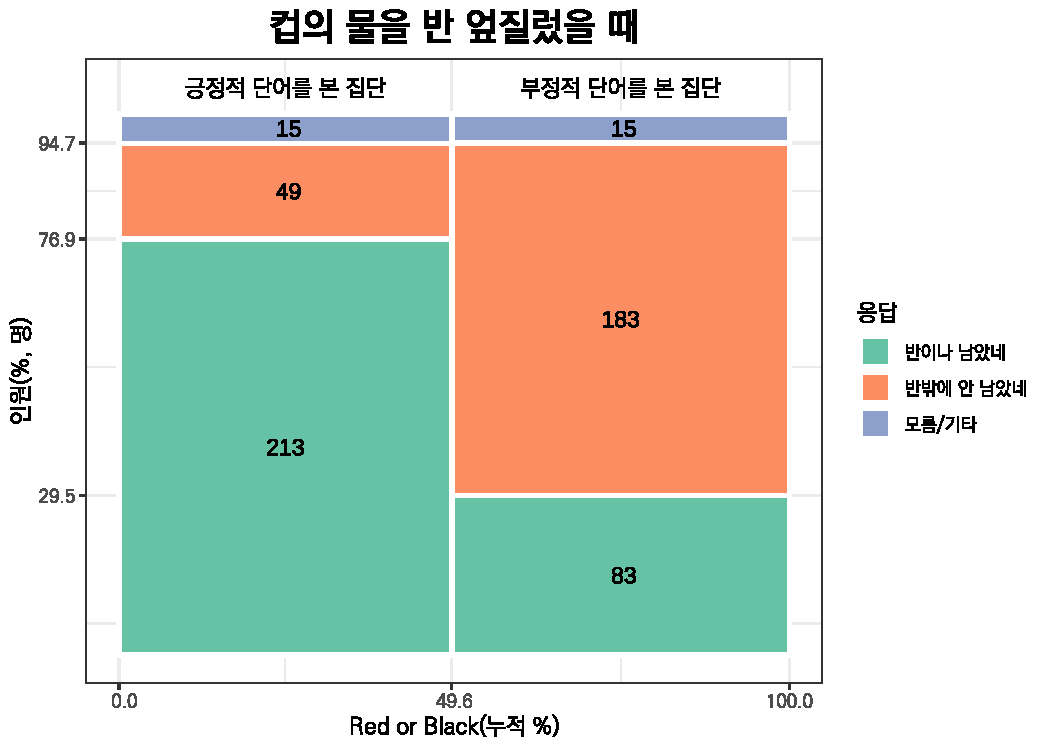
\includegraphics[keepaspectratio]{Quiz_report_2025_files/figure-latex/unnamed-chunk-116-1.pdf}}

Mosaic Plot 은 이 집계결과를 시각적으로 잘 보여줍니다. 긍정적 단어를 본 Red 에서 ``반이나'' 남아 있다고 응답한 백분율이 월등히 높고, 부정적 단어를 본 Black 에서 ``반 밖에'' 안 남았다고 응답한 백분율이 월등히 높은 것을 시각적으로 알 수 있습니다.

덤으로 ``모름/기타''의 백분율은 Red, Black 간에 매우 닮았다는 점도 시각적으로 쉽게 파악할 수 있습니다.

\section{마감 시간으로부터 제출 시간의 분포}\label{uxb9c8uxac10-uxc2dcuxac04uxc73cuxb85cuxbd80uxd130-uxc81cuxcd9c-uxc2dcuxac04uxc758-uxbd84uxd3ec-4}

\subsection{분포표}\label{uxbd84uxd3ecuxd45c-4}

\begin{longtable}[]{@{}
  >{\raggedright\arraybackslash}p{(\linewidth - 30\tabcolsep) * \real{0.1121}}
  >{\centering\arraybackslash}p{(\linewidth - 30\tabcolsep) * \real{0.0654}}
  >{\centering\arraybackslash}p{(\linewidth - 30\tabcolsep) * \real{0.0654}}
  >{\centering\arraybackslash}p{(\linewidth - 30\tabcolsep) * \real{0.0654}}
  >{\centering\arraybackslash}p{(\linewidth - 30\tabcolsep) * \real{0.0654}}
  >{\centering\arraybackslash}p{(\linewidth - 30\tabcolsep) * \real{0.0654}}
  >{\centering\arraybackslash}p{(\linewidth - 30\tabcolsep) * \real{0.0561}}
  >{\centering\arraybackslash}p{(\linewidth - 30\tabcolsep) * \real{0.0561}}
  >{\centering\arraybackslash}p{(\linewidth - 30\tabcolsep) * \real{0.0561}}
  >{\centering\arraybackslash}p{(\linewidth - 30\tabcolsep) * \real{0.0561}}
  >{\centering\arraybackslash}p{(\linewidth - 30\tabcolsep) * \real{0.0561}}
  >{\centering\arraybackslash}p{(\linewidth - 30\tabcolsep) * \real{0.0561}}
  >{\centering\arraybackslash}p{(\linewidth - 30\tabcolsep) * \real{0.0561}}
  >{\centering\arraybackslash}p{(\linewidth - 30\tabcolsep) * \real{0.0561}}
  >{\centering\arraybackslash}p{(\linewidth - 30\tabcolsep) * \real{0.0561}}
  >{\centering\arraybackslash}p{(\linewidth - 30\tabcolsep) * \real{0.0561}}@{}}
\caption{일 단위}\tabularnewline
\toprule\noalign{}
\begin{minipage}[b]{\linewidth}\raggedright
~
\end{minipage} & \begin{minipage}[b]{\linewidth}\centering
14일
\end{minipage} & \begin{minipage}[b]{\linewidth}\centering
13일
\end{minipage} & \begin{minipage}[b]{\linewidth}\centering
12일
\end{minipage} & \begin{minipage}[b]{\linewidth}\centering
11일
\end{minipage} & \begin{minipage}[b]{\linewidth}\centering
10일
\end{minipage} & \begin{minipage}[b]{\linewidth}\centering
9일
\end{minipage} & \begin{minipage}[b]{\linewidth}\centering
8일
\end{minipage} & \begin{minipage}[b]{\linewidth}\centering
7일
\end{minipage} & \begin{minipage}[b]{\linewidth}\centering
6일
\end{minipage} & \begin{minipage}[b]{\linewidth}\centering
5일
\end{minipage} & \begin{minipage}[b]{\linewidth}\centering
4일
\end{minipage} & \begin{minipage}[b]{\linewidth}\centering
3일
\end{minipage} & \begin{minipage}[b]{\linewidth}\centering
2일
\end{minipage} & \begin{minipage}[b]{\linewidth}\centering
1일
\end{minipage} & \begin{minipage}[b]{\linewidth}\centering
계
\end{minipage} \\
\midrule\noalign{}
\endfirsthead
\toprule\noalign{}
\begin{minipage}[b]{\linewidth}\raggedright
~
\end{minipage} & \begin{minipage}[b]{\linewidth}\centering
14일
\end{minipage} & \begin{minipage}[b]{\linewidth}\centering
13일
\end{minipage} & \begin{minipage}[b]{\linewidth}\centering
12일
\end{minipage} & \begin{minipage}[b]{\linewidth}\centering
11일
\end{minipage} & \begin{minipage}[b]{\linewidth}\centering
10일
\end{minipage} & \begin{minipage}[b]{\linewidth}\centering
9일
\end{minipage} & \begin{minipage}[b]{\linewidth}\centering
8일
\end{minipage} & \begin{minipage}[b]{\linewidth}\centering
7일
\end{minipage} & \begin{minipage}[b]{\linewidth}\centering
6일
\end{minipage} & \begin{minipage}[b]{\linewidth}\centering
5일
\end{minipage} & \begin{minipage}[b]{\linewidth}\centering
4일
\end{minipage} & \begin{minipage}[b]{\linewidth}\centering
3일
\end{minipage} & \begin{minipage}[b]{\linewidth}\centering
2일
\end{minipage} & \begin{minipage}[b]{\linewidth}\centering
1일
\end{minipage} & \begin{minipage}[b]{\linewidth}\centering
계
\end{minipage} \\
\midrule\noalign{}
\endhead
\bottomrule\noalign{}
\endlastfoot
\textbf{Red} & 81 & 14 & 8 & 13 & 11 & 5 & 4 & 38 & 22 & 13 & 14 & 19 & 12 & 23 & 277 \\
\textbf{Black} & 78 & 14 & 12 & 6 & 8 & 3 & 6 & 41 & 29 & 15 & 17 & 15 & 20 & 17 & 281 \\
\textbf{계} & 159 & 28 & 20 & 19 & 19 & 8 & 10 & 79 & 51 & 28 & 31 & 34 & 32 & 40 & 558 \\
\end{longtable}

분포표로부터 두 가지 문제를 살펴보겠습니다.

첫째, 날마다 고르게 제출하는가?

둘째, Red, Black 간에 통계적으로 유의한 차이가 있는가?

각 문제를 살펴보기 위해서는 분포표의 일부분을 대상으로 카이제곱 테스트를 수행합니다.

\subsection{날마다 고르게 제출하는가?}\label{uxb0a0uxb9c8uxb2e4-uxace0uxb974uxac8c-uxc81cuxcd9cuxd558uxb294uxac00-4}

\begin{longtable}[]{@{}
  >{\centering\arraybackslash}p{(\linewidth - 26\tabcolsep) * \real{0.0787}}
  >{\centering\arraybackslash}p{(\linewidth - 26\tabcolsep) * \real{0.0787}}
  >{\centering\arraybackslash}p{(\linewidth - 26\tabcolsep) * \real{0.0787}}
  >{\centering\arraybackslash}p{(\linewidth - 26\tabcolsep) * \real{0.0787}}
  >{\centering\arraybackslash}p{(\linewidth - 26\tabcolsep) * \real{0.0787}}
  >{\centering\arraybackslash}p{(\linewidth - 26\tabcolsep) * \real{0.0674}}
  >{\centering\arraybackslash}p{(\linewidth - 26\tabcolsep) * \real{0.0674}}
  >{\centering\arraybackslash}p{(\linewidth - 26\tabcolsep) * \real{0.0674}}
  >{\centering\arraybackslash}p{(\linewidth - 26\tabcolsep) * \real{0.0674}}
  >{\centering\arraybackslash}p{(\linewidth - 26\tabcolsep) * \real{0.0674}}
  >{\centering\arraybackslash}p{(\linewidth - 26\tabcolsep) * \real{0.0674}}
  >{\centering\arraybackslash}p{(\linewidth - 26\tabcolsep) * \real{0.0674}}
  >{\centering\arraybackslash}p{(\linewidth - 26\tabcolsep) * \real{0.0674}}
  >{\centering\arraybackslash}p{(\linewidth - 26\tabcolsep) * \real{0.0674}}@{}}
\toprule\noalign{}
\begin{minipage}[b]{\linewidth}\centering
14일
\end{minipage} & \begin{minipage}[b]{\linewidth}\centering
13일
\end{minipage} & \begin{minipage}[b]{\linewidth}\centering
12일
\end{minipage} & \begin{minipage}[b]{\linewidth}\centering
11일
\end{minipage} & \begin{minipage}[b]{\linewidth}\centering
10일
\end{minipage} & \begin{minipage}[b]{\linewidth}\centering
9일
\end{minipage} & \begin{minipage}[b]{\linewidth}\centering
8일
\end{minipage} & \begin{minipage}[b]{\linewidth}\centering
7일
\end{minipage} & \begin{minipage}[b]{\linewidth}\centering
6일
\end{minipage} & \begin{minipage}[b]{\linewidth}\centering
5일
\end{minipage} & \begin{minipage}[b]{\linewidth}\centering
4일
\end{minipage} & \begin{minipage}[b]{\linewidth}\centering
3일
\end{minipage} & \begin{minipage}[b]{\linewidth}\centering
2일
\end{minipage} & \begin{minipage}[b]{\linewidth}\centering
1일
\end{minipage} \\
\midrule\noalign{}
\endhead
\bottomrule\noalign{}
\endlastfoot
159 & 28 & 20 & 19 & 19 & 8 & 10 & 79 & 51 & 28 & 31 & 34 & 32 & 40 \\
\end{longtable}

\begin{longtable}[]{@{}
  >{\raggedleft\arraybackslash}p{(\linewidth - 4\tabcolsep) * \real{0.2361}}
  >{\raggedleft\arraybackslash}p{(\linewidth - 4\tabcolsep) * \real{0.0694}}
  >{\raggedleft\arraybackslash}p{(\linewidth - 4\tabcolsep) * \real{0.2500}}@{}}
\caption{Chi-squared test for given probabilities: \texttt{.}}\tabularnewline
\toprule\noalign{}
\begin{minipage}[b]{\linewidth}\raggedleft
Test statistic
\end{minipage} & \begin{minipage}[b]{\linewidth}\raggedleft
df
\end{minipage} & \begin{minipage}[b]{\linewidth}\raggedleft
P value
\end{minipage} \\
\midrule\noalign{}
\endfirsthead
\toprule\noalign{}
\begin{minipage}[b]{\linewidth}\raggedleft
Test statistic
\end{minipage} & \begin{minipage}[b]{\linewidth}\raggedleft
df
\end{minipage} & \begin{minipage}[b]{\linewidth}\raggedleft
P value
\end{minipage} \\
\midrule\noalign{}
\endhead
\bottomrule\noalign{}
\endlastfoot
488.7 & 13 & 3.693e-96 * * * \\
\end{longtable}

날마다 고르게 제출하는지 알아 보았습니다.

분포표의 ``계''행에서 '계'열을 제외하고 카이제곱테스트를 수행합니다. 분포표 만으로도 쉽게 파악할 수 있지만 카이제곱테스트가 명확히 해 줍니다.

카이제곱 통계량은 488.69, 자유도는 13.00, p-value 는 3.7e-96 이므로 결코 고르게 제출한다고 말할 수 없겠습니다.

막대그래프로 살펴 보겠습니다.

\subsection{막대그래프}\label{uxb9c9uxb300uxadf8uxb798uxd504-4}

\pandocbounded{\includegraphics[keepaspectratio]{Quiz_report_2025_files/figure-latex/unnamed-chunk-119-1.pdf}}

막대그래프는 총 제출인원 558(명) 중에 159(명), 28(\%)가 마감일에 몰리는 것을 명확히 보여주고 있습니다.

\subsection{Red, Black 간에 닮았는가?}\label{red-black-uxac04uxc5d0-uxb2eeuxc558uxb294uxac00-4}

\begin{longtable}[]{@{}
  >{\raggedright\arraybackslash}p{(\linewidth - 28\tabcolsep) * \real{0.1188}}
  >{\centering\arraybackslash}p{(\linewidth - 28\tabcolsep) * \real{0.0693}}
  >{\centering\arraybackslash}p{(\linewidth - 28\tabcolsep) * \real{0.0693}}
  >{\centering\arraybackslash}p{(\linewidth - 28\tabcolsep) * \real{0.0693}}
  >{\centering\arraybackslash}p{(\linewidth - 28\tabcolsep) * \real{0.0693}}
  >{\centering\arraybackslash}p{(\linewidth - 28\tabcolsep) * \real{0.0693}}
  >{\centering\arraybackslash}p{(\linewidth - 28\tabcolsep) * \real{0.0594}}
  >{\centering\arraybackslash}p{(\linewidth - 28\tabcolsep) * \real{0.0594}}
  >{\centering\arraybackslash}p{(\linewidth - 28\tabcolsep) * \real{0.0594}}
  >{\centering\arraybackslash}p{(\linewidth - 28\tabcolsep) * \real{0.0594}}
  >{\centering\arraybackslash}p{(\linewidth - 28\tabcolsep) * \real{0.0594}}
  >{\centering\arraybackslash}p{(\linewidth - 28\tabcolsep) * \real{0.0594}}
  >{\centering\arraybackslash}p{(\linewidth - 28\tabcolsep) * \real{0.0594}}
  >{\centering\arraybackslash}p{(\linewidth - 28\tabcolsep) * \real{0.0594}}
  >{\centering\arraybackslash}p{(\linewidth - 28\tabcolsep) * \real{0.0594}}@{}}
\toprule\noalign{}
\begin{minipage}[b]{\linewidth}\raggedright
~
\end{minipage} & \begin{minipage}[b]{\linewidth}\centering
14일
\end{minipage} & \begin{minipage}[b]{\linewidth}\centering
13일
\end{minipage} & \begin{minipage}[b]{\linewidth}\centering
12일
\end{minipage} & \begin{minipage}[b]{\linewidth}\centering
11일
\end{minipage} & \begin{minipage}[b]{\linewidth}\centering
10일
\end{minipage} & \begin{minipage}[b]{\linewidth}\centering
9일
\end{minipage} & \begin{minipage}[b]{\linewidth}\centering
8일
\end{minipage} & \begin{minipage}[b]{\linewidth}\centering
7일
\end{minipage} & \begin{minipage}[b]{\linewidth}\centering
6일
\end{minipage} & \begin{minipage}[b]{\linewidth}\centering
5일
\end{minipage} & \begin{minipage}[b]{\linewidth}\centering
4일
\end{minipage} & \begin{minipage}[b]{\linewidth}\centering
3일
\end{minipage} & \begin{minipage}[b]{\linewidth}\centering
2일
\end{minipage} & \begin{minipage}[b]{\linewidth}\centering
1일
\end{minipage} \\
\midrule\noalign{}
\endhead
\bottomrule\noalign{}
\endlastfoot
\textbf{Red} & 81 & 14 & 8 & 13 & 11 & 5 & 4 & 38 & 22 & 13 & 14 & 19 & 12 & 23 \\
\textbf{Black} & 78 & 14 & 12 & 6 & 8 & 3 & 6 & 41 & 29 & 15 & 17 & 15 & 20 & 17 \\
\end{longtable}

\begin{longtable}[]{@{}
  >{\raggedleft\arraybackslash}p{(\linewidth - 4\tabcolsep) * \real{0.2361}}
  >{\raggedleft\arraybackslash}p{(\linewidth - 4\tabcolsep) * \real{0.0694}}
  >{\raggedleft\arraybackslash}p{(\linewidth - 4\tabcolsep) * \real{0.1389}}@{}}
\caption{Pearson's Chi-squared test: \texttt{.}}\tabularnewline
\toprule\noalign{}
\begin{minipage}[b]{\linewidth}\raggedleft
Test statistic
\end{minipage} & \begin{minipage}[b]{\linewidth}\raggedleft
df
\end{minipage} & \begin{minipage}[b]{\linewidth}\raggedleft
P value
\end{minipage} \\
\midrule\noalign{}
\endfirsthead
\toprule\noalign{}
\begin{minipage}[b]{\linewidth}\raggedleft
Test statistic
\end{minipage} & \begin{minipage}[b]{\linewidth}\raggedleft
df
\end{minipage} & \begin{minipage}[b]{\linewidth}\raggedleft
P value
\end{minipage} \\
\midrule\noalign{}
\endhead
\bottomrule\noalign{}
\endlastfoot
9.66 & 13 & 0.7215 \\
\end{longtable}

제출시간의 분포가 Red, Black 간에 닮았는지 알아 보았습니다.

이번에는 분포표의 첫번째와 두번째 행, '계'열을 제외한 나머지 열에 대해서 카이제곱테스트를 수행합니다.

카이제곱 통계량은 9.660, 자유도는 13, p-value 는 0.7215 이므로 제출 시간의 분포는 Red, Black 간에 통계적으로 유의한 차이가 관찰되지 않습니다.

이 사실을 Mosaic Plot을 이용하여 시각적으로 살펴보겠습니다.

닮았다고 느껴지나요?

\subsection{Mosaic Plot}\label{mosaic-plot-9}

\pandocbounded{\includegraphics[keepaspectratio]{Quiz_report_2025_files/figure-latex/unnamed-chunk-121-1.pdf}}

\chapter{국민문해력조사 집계 결과}\label{uxad6duxbbfcuxbb38uxd574uxb825uxc870uxc0ac-uxc9d1uxacc4-uxacb0uxacfc}

\section{응답 집계}\label{uxc751uxb2f5-uxc9d1uxacc4}

\begin{longtable}[]{@{}
  >{\raggedright\arraybackslash}p{(\linewidth - 48\tabcolsep) * \real{0.0400}}
  >{\raggedright\arraybackslash}p{(\linewidth - 48\tabcolsep) * \real{0.0400}}
  >{\raggedright\arraybackslash}p{(\linewidth - 48\tabcolsep) * \real{0.0400}}
  >{\raggedright\arraybackslash}p{(\linewidth - 48\tabcolsep) * \real{0.0400}}
  >{\raggedright\arraybackslash}p{(\linewidth - 48\tabcolsep) * \real{0.0400}}
  >{\raggedright\arraybackslash}p{(\linewidth - 48\tabcolsep) * \real{0.0400}}
  >{\raggedright\arraybackslash}p{(\linewidth - 48\tabcolsep) * \real{0.0400}}
  >{\raggedright\arraybackslash}p{(\linewidth - 48\tabcolsep) * \real{0.0400}}
  >{\raggedright\arraybackslash}p{(\linewidth - 48\tabcolsep) * \real{0.0400}}
  >{\raggedright\arraybackslash}p{(\linewidth - 48\tabcolsep) * \real{0.0400}}
  >{\raggedright\arraybackslash}p{(\linewidth - 48\tabcolsep) * \real{0.0400}}
  >{\raggedright\arraybackslash}p{(\linewidth - 48\tabcolsep) * \real{0.0400}}
  >{\raggedright\arraybackslash}p{(\linewidth - 48\tabcolsep) * \real{0.0400}}
  >{\raggedright\arraybackslash}p{(\linewidth - 48\tabcolsep) * \real{0.0400}}
  >{\raggedright\arraybackslash}p{(\linewidth - 48\tabcolsep) * \real{0.0400}}
  >{\raggedright\arraybackslash}p{(\linewidth - 48\tabcolsep) * \real{0.0400}}
  >{\raggedright\arraybackslash}p{(\linewidth - 48\tabcolsep) * \real{0.0400}}
  >{\raggedright\arraybackslash}p{(\linewidth - 48\tabcolsep) * \real{0.0400}}
  >{\raggedright\arraybackslash}p{(\linewidth - 48\tabcolsep) * \real{0.0400}}
  >{\raggedright\arraybackslash}p{(\linewidth - 48\tabcolsep) * \real{0.0400}}
  >{\raggedright\arraybackslash}p{(\linewidth - 48\tabcolsep) * \real{0.0400}}
  >{\raggedright\arraybackslash}p{(\linewidth - 48\tabcolsep) * \real{0.0400}}
  >{\raggedright\arraybackslash}p{(\linewidth - 48\tabcolsep) * \real{0.0400}}
  >{\raggedright\arraybackslash}p{(\linewidth - 48\tabcolsep) * \real{0.0400}}
  >{\raggedright\arraybackslash}p{(\linewidth - 48\tabcolsep) * \real{0.0400}}@{}}
\caption{Counts}\tabularnewline
\toprule\noalign{}
\begin{minipage}[b]{\linewidth}\raggedright
Q1
\end{minipage} & \begin{minipage}[b]{\linewidth}\raggedright
Q2
\end{minipage} & \begin{minipage}[b]{\linewidth}\raggedright
Q3
\end{minipage} & \begin{minipage}[b]{\linewidth}\raggedright
Q4
\end{minipage} & \begin{minipage}[b]{\linewidth}\raggedright
Q5
\end{minipage} & \begin{minipage}[b]{\linewidth}\raggedright
Q6
\end{minipage} & \begin{minipage}[b]{\linewidth}\raggedright
Q7
\end{minipage} & \begin{minipage}[b]{\linewidth}\raggedright
Q8
\end{minipage} & \begin{minipage}[b]{\linewidth}\raggedright
Q9
\end{minipage} & \begin{minipage}[b]{\linewidth}\raggedright
Q10
\end{minipage} & \begin{minipage}[b]{\linewidth}\raggedright
Q11
\end{minipage} & \begin{minipage}[b]{\linewidth}\raggedright
Q12
\end{minipage} & \begin{minipage}[b]{\linewidth}\raggedright
Q13
\end{minipage} & \begin{minipage}[b]{\linewidth}\raggedright
Q14
\end{minipage} & \begin{minipage}[b]{\linewidth}\raggedright
Q15
\end{minipage} & \begin{minipage}[b]{\linewidth}\raggedright
Q16
\end{minipage} & \begin{minipage}[b]{\linewidth}\raggedright
Q17
\end{minipage} & \begin{minipage}[b]{\linewidth}\raggedright
Q18
\end{minipage} & \begin{minipage}[b]{\linewidth}\raggedright
Q19
\end{minipage} & \begin{minipage}[b]{\linewidth}\raggedright
Q20
\end{minipage} & \begin{minipage}[b]{\linewidth}\raggedright
Q21
\end{minipage} & \begin{minipage}[b]{\linewidth}\raggedright
Q22
\end{minipage} & \begin{minipage}[b]{\linewidth}\raggedright
Q23
\end{minipage} & \begin{minipage}[b]{\linewidth}\raggedright
Q24
\end{minipage} & \begin{minipage}[b]{\linewidth}\raggedright
Q25
\end{minipage} \\
\midrule\noalign{}
\endfirsthead
\toprule\noalign{}
\begin{minipage}[b]{\linewidth}\raggedright
Q1
\end{minipage} & \begin{minipage}[b]{\linewidth}\raggedright
Q2
\end{minipage} & \begin{minipage}[b]{\linewidth}\raggedright
Q3
\end{minipage} & \begin{minipage}[b]{\linewidth}\raggedright
Q4
\end{minipage} & \begin{minipage}[b]{\linewidth}\raggedright
Q5
\end{minipage} & \begin{minipage}[b]{\linewidth}\raggedright
Q6
\end{minipage} & \begin{minipage}[b]{\linewidth}\raggedright
Q7
\end{minipage} & \begin{minipage}[b]{\linewidth}\raggedright
Q8
\end{minipage} & \begin{minipage}[b]{\linewidth}\raggedright
Q9
\end{minipage} & \begin{minipage}[b]{\linewidth}\raggedright
Q10
\end{minipage} & \begin{minipage}[b]{\linewidth}\raggedright
Q11
\end{minipage} & \begin{minipage}[b]{\linewidth}\raggedright
Q12
\end{minipage} & \begin{minipage}[b]{\linewidth}\raggedright
Q13
\end{minipage} & \begin{minipage}[b]{\linewidth}\raggedright
Q14
\end{minipage} & \begin{minipage}[b]{\linewidth}\raggedright
Q15
\end{minipage} & \begin{minipage}[b]{\linewidth}\raggedright
Q16
\end{minipage} & \begin{minipage}[b]{\linewidth}\raggedright
Q17
\end{minipage} & \begin{minipage}[b]{\linewidth}\raggedright
Q18
\end{minipage} & \begin{minipage}[b]{\linewidth}\raggedright
Q19
\end{minipage} & \begin{minipage}[b]{\linewidth}\raggedright
Q20
\end{minipage} & \begin{minipage}[b]{\linewidth}\raggedright
Q21
\end{minipage} & \begin{minipage}[b]{\linewidth}\raggedright
Q22
\end{minipage} & \begin{minipage}[b]{\linewidth}\raggedright
Q23
\end{minipage} & \begin{minipage}[b]{\linewidth}\raggedright
Q24
\end{minipage} & \begin{minipage}[b]{\linewidth}\raggedright
Q25
\end{minipage} \\
\midrule\noalign{}
\endhead
\bottomrule\noalign{}
\endlastfoot
0 & 5 & 420 & 7 & 6 & 43 & 502 & 37 & 47 & 8 & 480 & 17 & 10 & 18 & 22 & 443 & 137 & 11 & 495 & 34 & 25 & 33 & 487 & 56 & 15 \\
8 & 3 & 31 & 8 & 482 & 38 & 17 & 35 & 297 & 483 & 24 & 153 & 474 & 30 & 59 & 44 & 33 & 492 & 16 & 52 & 440 & 68 & 26 & 28 & 441 \\
537 & 27 & 19 & 521 & 44 & 90 & 17 & 39 & 186 & 31 & 27 & 362 & 30 & 21 & 395 & 37 & 21 & 37 & 20 & 441 & 31 & 45 & 17 & 435 & 69 \\
1 & 511 & 76 & 10 & 14 & 375 & 10 & 435 & 16 & 24 & 15 & 14 & 32 & 477 & 70 & 22 & 355 & 6 & 15 & 19 & 50 & 400 & 16 & 27 & 21 \\
\end{longtable}

\begin{longtable}[]{@{}
  >{\raggedright\arraybackslash}p{(\linewidth - 48\tabcolsep) * \real{0.0355}}
  >{\raggedright\arraybackslash}p{(\linewidth - 48\tabcolsep) * \real{0.0355}}
  >{\raggedright\arraybackslash}p{(\linewidth - 48\tabcolsep) * \real{0.0355}}
  >{\raggedright\arraybackslash}p{(\linewidth - 48\tabcolsep) * \real{0.0355}}
  >{\raggedright\arraybackslash}p{(\linewidth - 48\tabcolsep) * \real{0.0355}}
  >{\raggedright\arraybackslash}p{(\linewidth - 48\tabcolsep) * \real{0.0355}}
  >{\raggedright\arraybackslash}p{(\linewidth - 48\tabcolsep) * \real{0.0355}}
  >{\raggedright\arraybackslash}p{(\linewidth - 48\tabcolsep) * \real{0.0355}}
  >{\raggedright\arraybackslash}p{(\linewidth - 48\tabcolsep) * \real{0.0355}}
  >{\raggedright\arraybackslash}p{(\linewidth - 48\tabcolsep) * \real{0.0426}}
  >{\raggedright\arraybackslash}p{(\linewidth - 48\tabcolsep) * \real{0.0426}}
  >{\raggedright\arraybackslash}p{(\linewidth - 48\tabcolsep) * \real{0.0426}}
  >{\raggedright\arraybackslash}p{(\linewidth - 48\tabcolsep) * \real{0.0426}}
  >{\raggedright\arraybackslash}p{(\linewidth - 48\tabcolsep) * \real{0.0426}}
  >{\raggedright\arraybackslash}p{(\linewidth - 48\tabcolsep) * \real{0.0426}}
  >{\raggedright\arraybackslash}p{(\linewidth - 48\tabcolsep) * \real{0.0426}}
  >{\raggedright\arraybackslash}p{(\linewidth - 48\tabcolsep) * \real{0.0426}}
  >{\raggedright\arraybackslash}p{(\linewidth - 48\tabcolsep) * \real{0.0426}}
  >{\raggedright\arraybackslash}p{(\linewidth - 48\tabcolsep) * \real{0.0426}}
  >{\raggedright\arraybackslash}p{(\linewidth - 48\tabcolsep) * \real{0.0426}}
  >{\raggedright\arraybackslash}p{(\linewidth - 48\tabcolsep) * \real{0.0426}}
  >{\raggedright\arraybackslash}p{(\linewidth - 48\tabcolsep) * \real{0.0426}}
  >{\raggedright\arraybackslash}p{(\linewidth - 48\tabcolsep) * \real{0.0426}}
  >{\raggedright\arraybackslash}p{(\linewidth - 48\tabcolsep) * \real{0.0426}}
  >{\raggedright\arraybackslash}p{(\linewidth - 48\tabcolsep) * \real{0.0426}}@{}}
\caption{\%}\tabularnewline
\toprule\noalign{}
\begin{minipage}[b]{\linewidth}\raggedright
Q1
\end{minipage} & \begin{minipage}[b]{\linewidth}\raggedright
Q2
\end{minipage} & \begin{minipage}[b]{\linewidth}\raggedright
Q3
\end{minipage} & \begin{minipage}[b]{\linewidth}\raggedright
Q4
\end{minipage} & \begin{minipage}[b]{\linewidth}\raggedright
Q5
\end{minipage} & \begin{minipage}[b]{\linewidth}\raggedright
Q6
\end{minipage} & \begin{minipage}[b]{\linewidth}\raggedright
Q7
\end{minipage} & \begin{minipage}[b]{\linewidth}\raggedright
Q8
\end{minipage} & \begin{minipage}[b]{\linewidth}\raggedright
Q9
\end{minipage} & \begin{minipage}[b]{\linewidth}\raggedright
Q10
\end{minipage} & \begin{minipage}[b]{\linewidth}\raggedright
Q11
\end{minipage} & \begin{minipage}[b]{\linewidth}\raggedright
Q12
\end{minipage} & \begin{minipage}[b]{\linewidth}\raggedright
Q13
\end{minipage} & \begin{minipage}[b]{\linewidth}\raggedright
Q14
\end{minipage} & \begin{minipage}[b]{\linewidth}\raggedright
Q15
\end{minipage} & \begin{minipage}[b]{\linewidth}\raggedright
Q16
\end{minipage} & \begin{minipage}[b]{\linewidth}\raggedright
Q17
\end{minipage} & \begin{minipage}[b]{\linewidth}\raggedright
Q18
\end{minipage} & \begin{minipage}[b]{\linewidth}\raggedright
Q19
\end{minipage} & \begin{minipage}[b]{\linewidth}\raggedright
Q20
\end{minipage} & \begin{minipage}[b]{\linewidth}\raggedright
Q21
\end{minipage} & \begin{minipage}[b]{\linewidth}\raggedright
Q22
\end{minipage} & \begin{minipage}[b]{\linewidth}\raggedright
Q23
\end{minipage} & \begin{minipage}[b]{\linewidth}\raggedright
Q24
\end{minipage} & \begin{minipage}[b]{\linewidth}\raggedright
Q25
\end{minipage} \\
\midrule\noalign{}
\endfirsthead
\toprule\noalign{}
\begin{minipage}[b]{\linewidth}\raggedright
Q1
\end{minipage} & \begin{minipage}[b]{\linewidth}\raggedright
Q2
\end{minipage} & \begin{minipage}[b]{\linewidth}\raggedright
Q3
\end{minipage} & \begin{minipage}[b]{\linewidth}\raggedright
Q4
\end{minipage} & \begin{minipage}[b]{\linewidth}\raggedright
Q5
\end{minipage} & \begin{minipage}[b]{\linewidth}\raggedright
Q6
\end{minipage} & \begin{minipage}[b]{\linewidth}\raggedright
Q7
\end{minipage} & \begin{minipage}[b]{\linewidth}\raggedright
Q8
\end{minipage} & \begin{minipage}[b]{\linewidth}\raggedright
Q9
\end{minipage} & \begin{minipage}[b]{\linewidth}\raggedright
Q10
\end{minipage} & \begin{minipage}[b]{\linewidth}\raggedright
Q11
\end{minipage} & \begin{minipage}[b]{\linewidth}\raggedright
Q12
\end{minipage} & \begin{minipage}[b]{\linewidth}\raggedright
Q13
\end{minipage} & \begin{minipage}[b]{\linewidth}\raggedright
Q14
\end{minipage} & \begin{minipage}[b]{\linewidth}\raggedright
Q15
\end{minipage} & \begin{minipage}[b]{\linewidth}\raggedright
Q16
\end{minipage} & \begin{minipage}[b]{\linewidth}\raggedright
Q17
\end{minipage} & \begin{minipage}[b]{\linewidth}\raggedright
Q18
\end{minipage} & \begin{minipage}[b]{\linewidth}\raggedright
Q19
\end{minipage} & \begin{minipage}[b]{\linewidth}\raggedright
Q20
\end{minipage} & \begin{minipage}[b]{\linewidth}\raggedright
Q21
\end{minipage} & \begin{minipage}[b]{\linewidth}\raggedright
Q22
\end{minipage} & \begin{minipage}[b]{\linewidth}\raggedright
Q23
\end{minipage} & \begin{minipage}[b]{\linewidth}\raggedright
Q24
\end{minipage} & \begin{minipage}[b]{\linewidth}\raggedright
Q25
\end{minipage} \\
\midrule\noalign{}
\endhead
\bottomrule\noalign{}
\endlastfoot
0 & 1 & 77 & 1 & 1 & 8 & 92 & 7 & 9 & 1 & 88 & 3 & 2 & 3 & 4 & 81 & 25 & 2 & 91 & 6 & 5 & 6 & 89 & 10 & 3 \\
1 & 1 & 6 & 1 & 88 & 7 & 3 & 6 & 54 & 88 & 4 & 28 & 87 & 5 & 11 & 8 & 6 & 90 & 3 & 10 & 81 & 12 & 5 & 5 & 81 \\
98 & 5 & 3 & 95 & 8 & 16 & 3 & 7 & 34 & 6 & 5 & 66 & 5 & 4 & 72 & 7 & 4 & 7 & 4 & 81 & 6 & 8 & 3 & 80 & 13 \\
0 & 94 & 14 & 2 & 3 & 69 & 2 & 80 & 3 & 4 & 3 & 3 & 6 & 87 & 13 & 4 & 65 & 1 & 3 & 3 & 9 & 73 & 3 & 5 & 4 \\
\end{longtable}

\section{막대그래프}\label{uxb9c9uxb300uxadf8uxb798uxd504-5}

막대그래프로 답안 분포를 시각적으로 살핀다. 차후 나오는 정답률과 함께 어느 문항에서 어느 답안을 많이 고르는지 파악하는 데 활용한다.

\pandocbounded{\includegraphics[keepaspectratio]{Quiz_report_2025_files/figure-latex/unnamed-chunk-127-1.pdf}}

\section{문해력 점수 계산}\label{uxbb38uxd574uxb825-uxc810uxc218-uxacc4uxc0b0}

\subsection{정답과 대조하여 R(Right)/W(Wrong) 표시}\label{uxc815uxb2f5uxacfc-uxb300uxc870uxd558uxc5ec-rrightwwrong-uxd45cuxc2dc}

\begin{longtable}[]{@{}
  >{\raggedright\arraybackslash}p{(\linewidth - 48\tabcolsep) * \real{0.0355}}
  >{\raggedright\arraybackslash}p{(\linewidth - 48\tabcolsep) * \real{0.0355}}
  >{\raggedright\arraybackslash}p{(\linewidth - 48\tabcolsep) * \real{0.0355}}
  >{\raggedright\arraybackslash}p{(\linewidth - 48\tabcolsep) * \real{0.0355}}
  >{\raggedright\arraybackslash}p{(\linewidth - 48\tabcolsep) * \real{0.0355}}
  >{\raggedright\arraybackslash}p{(\linewidth - 48\tabcolsep) * \real{0.0355}}
  >{\raggedright\arraybackslash}p{(\linewidth - 48\tabcolsep) * \real{0.0355}}
  >{\raggedright\arraybackslash}p{(\linewidth - 48\tabcolsep) * \real{0.0355}}
  >{\raggedright\arraybackslash}p{(\linewidth - 48\tabcolsep) * \real{0.0355}}
  >{\raggedright\arraybackslash}p{(\linewidth - 48\tabcolsep) * \real{0.0426}}
  >{\raggedright\arraybackslash}p{(\linewidth - 48\tabcolsep) * \real{0.0426}}
  >{\raggedright\arraybackslash}p{(\linewidth - 48\tabcolsep) * \real{0.0426}}
  >{\raggedright\arraybackslash}p{(\linewidth - 48\tabcolsep) * \real{0.0426}}
  >{\raggedright\arraybackslash}p{(\linewidth - 48\tabcolsep) * \real{0.0426}}
  >{\raggedright\arraybackslash}p{(\linewidth - 48\tabcolsep) * \real{0.0426}}
  >{\raggedright\arraybackslash}p{(\linewidth - 48\tabcolsep) * \real{0.0426}}
  >{\raggedright\arraybackslash}p{(\linewidth - 48\tabcolsep) * \real{0.0426}}
  >{\raggedright\arraybackslash}p{(\linewidth - 48\tabcolsep) * \real{0.0426}}
  >{\raggedright\arraybackslash}p{(\linewidth - 48\tabcolsep) * \real{0.0426}}
  >{\raggedright\arraybackslash}p{(\linewidth - 48\tabcolsep) * \real{0.0426}}
  >{\raggedright\arraybackslash}p{(\linewidth - 48\tabcolsep) * \real{0.0426}}
  >{\raggedright\arraybackslash}p{(\linewidth - 48\tabcolsep) * \real{0.0426}}
  >{\raggedright\arraybackslash}p{(\linewidth - 48\tabcolsep) * \real{0.0426}}
  >{\raggedright\arraybackslash}p{(\linewidth - 48\tabcolsep) * \real{0.0426}}
  >{\raggedright\arraybackslash}p{(\linewidth - 48\tabcolsep) * \real{0.0426}}@{}}
\toprule\noalign{}
\begin{minipage}[b]{\linewidth}\raggedright
Q1
\end{minipage} & \begin{minipage}[b]{\linewidth}\raggedright
Q2
\end{minipage} & \begin{minipage}[b]{\linewidth}\raggedright
Q3
\end{minipage} & \begin{minipage}[b]{\linewidth}\raggedright
Q4
\end{minipage} & \begin{minipage}[b]{\linewidth}\raggedright
Q5
\end{minipage} & \begin{minipage}[b]{\linewidth}\raggedright
Q6
\end{minipage} & \begin{minipage}[b]{\linewidth}\raggedright
Q7
\end{minipage} & \begin{minipage}[b]{\linewidth}\raggedright
Q8
\end{minipage} & \begin{minipage}[b]{\linewidth}\raggedright
Q9
\end{minipage} & \begin{minipage}[b]{\linewidth}\raggedright
Q10
\end{minipage} & \begin{minipage}[b]{\linewidth}\raggedright
Q11
\end{minipage} & \begin{minipage}[b]{\linewidth}\raggedright
Q12
\end{minipage} & \begin{minipage}[b]{\linewidth}\raggedright
Q13
\end{minipage} & \begin{minipage}[b]{\linewidth}\raggedright
Q14
\end{minipage} & \begin{minipage}[b]{\linewidth}\raggedright
Q15
\end{minipage} & \begin{minipage}[b]{\linewidth}\raggedright
Q16
\end{minipage} & \begin{minipage}[b]{\linewidth}\raggedright
Q17
\end{minipage} & \begin{minipage}[b]{\linewidth}\raggedright
Q18
\end{minipage} & \begin{minipage}[b]{\linewidth}\raggedright
Q19
\end{minipage} & \begin{minipage}[b]{\linewidth}\raggedright
Q20
\end{minipage} & \begin{minipage}[b]{\linewidth}\raggedright
Q21
\end{minipage} & \begin{minipage}[b]{\linewidth}\raggedright
Q22
\end{minipage} & \begin{minipage}[b]{\linewidth}\raggedright
Q23
\end{minipage} & \begin{minipage}[b]{\linewidth}\raggedright
Q24
\end{minipage} & \begin{minipage}[b]{\linewidth}\raggedright
Q25
\end{minipage} \\
\midrule\noalign{}
\endhead
\bottomrule\noalign{}
\endlastfoot
R & R & R & R & R & W & W & W & W & W & R & R & R & R & R & R & R & R & R & R & R & R & R & R & R \\
R & R & R & R & R & R & R & R & R & R & R & R & R & R & R & R & W & R & R & R & R & R & R & R & R \\
R & R & R & R & R & R & R & R & R & R & R & R & R & R & R & R & W & R & R & R & R & R & R & R & R \\
R & R & R & R & R & R & R & R & R & R & R & R & R & R & R & R & R & R & R & R & R & R & R & R & R \\
R & R & R & R & R & R & R & W & W & R & R & W & R & R & W & R & W & R & R & W & R & R & R & R & R \\
R & R & R & R & R & R & R & R & R & R & R & R & R & R & R & R & R & R & R & R & R & R & R & R & R \\
\end{longtable}

\subsection{학생별 점수 산출}\label{uxd559uxc0dduxbcc4-uxc810uxc218-uxc0b0uxcd9c}

\emph{80}, \emph{96}, \emph{96}, \emph{100}, \emph{76}, \emph{100}, \emph{88}, \emph{20}, \emph{92}, \emph{92}, \emph{88}, \emph{80}, \emph{100}, \emph{100}, \emph{80}, \emph{100}, \emph{92}, \emph{84}, \emph{100}, \emph{92}, \emph{84}, \emph{100}, \emph{92}, \emph{100}, \emph{96}, \emph{92}, \emph{84}, \emph{88}, \emph{48}, \emph{92}, \emph{96}, \emph{100}, \emph{80}, \emph{96}, \emph{92}, \emph{84}, \emph{92}, \emph{72}, \emph{96}, \emph{96}, \emph{96}, \emph{60}, \emph{100}, \emph{76}, \emph{76}, \emph{72}, \emph{80}, \emph{32}, \emph{64}, \emph{88}, \emph{92}, \emph{92}, \emph{92}, \emph{88}, \emph{96}, \emph{96}, \emph{48}, \emph{84}, \emph{72}, \emph{100}, \emph{88}, \emph{88}, \emph{88}, \emph{92}, \emph{76}, \emph{96}, \emph{96}, \emph{84}, \emph{92}, \emph{88}, \emph{96}, \emph{88}, \emph{100}, \emph{68}, \emph{80}, \emph{76}, \emph{84}, \emph{92}, \emph{92}, \emph{92}, \emph{80}, \emph{88}, \emph{84}, \emph{56}, \emph{72}, \emph{80}, \emph{84}, \emph{28}, \emph{100}, \emph{96}, \emph{92}, \emph{92}, \emph{88}, \emph{84}, \emph{88}, \emph{96}, \emph{84}, \emph{84}, \emph{88}, \emph{88}, \emph{92}, \emph{88}, \emph{88}, \emph{84}, \emph{76}, \emph{88}, \emph{88}, \emph{92}, \emph{44}, \emph{80}, \emph{84}, \emph{20}, \emph{80}, \emph{72}, \emph{92}, \emph{100}, \emph{96}, \emph{92}, \emph{88}, \emph{72}, \emph{88}, \emph{64}, \emph{56}, \emph{96}, \emph{80}, \emph{92}, \emph{84}, \emph{88}, \emph{76}, \emph{80}, \emph{84}, \emph{76}, \emph{88}, \emph{36}, \emph{80}, \emph{92}, \emph{84}, \emph{68}, \emph{80}, \emph{76}, \emph{80}, \emph{96}, \emph{96}, \emph{84}, \emph{96}, \emph{88}, \emph{68}, \emph{92}, \emph{92}, \emph{88}, \emph{92}, \emph{28}, \emph{80}, \emph{44}, \emph{100}, \emph{84}, \emph{84}, \emph{96}, \emph{68}, \emph{100}, \emph{88}, \emph{84}, \emph{92}, \emph{92}, \emph{100}, \emph{96}, \emph{92}, \emph{96}, \emph{12}, \emph{92}, \emph{72}, \emph{92}, \emph{88}, \emph{100}, \emph{20}, \emph{80}, \emph{92}, \emph{100}, \emph{100}, \emph{100}, \emph{92}, \emph{100}, \emph{92}, \emph{92}, \emph{80}, \emph{84}, \emph{92}, \emph{88}, \emph{88}, \emph{100}, \emph{88}, \emph{88}, \emph{96}, \emph{92}, \emph{80}, \emph{100}, \emph{92}, \emph{88}, \emph{96}, \emph{84}, \emph{96}, \emph{96}, \emph{96}, \emph{80}, \emph{96}, \emph{96}, \emph{52}, \emph{80}, \emph{84}, \emph{68}, \emph{92}, \emph{84}, \emph{80}, \emph{48}, \emph{84}, \emph{80}, \emph{88}, \emph{84}, \emph{96}, \emph{36}, \emph{88}, \emph{92}, \emph{88}, \emph{88}, \emph{60}, \emph{80}, \emph{84}, \emph{88}, \emph{92}, \emph{84}, \emph{64}, \emph{92}, \emph{92}, \emph{96}, \emph{88}, \emph{88}, \emph{88}, \emph{88}, \emph{88}, \emph{36}, \emph{64}, \emph{84}, \emph{76}, \emph{80}, \emph{80}, \emph{24}, \emph{100}, \emph{88}, \emph{80}, \emph{88}, \emph{92}, \emph{64}, \emph{76}, \emph{80}, \emph{24}, \emph{80}, \emph{96}, \emph{56}, \emph{64}, \emph{84}, \emph{88}, \emph{64}, \emph{84}, \emph{84}, \emph{96}, \emph{84}, \emph{92}, \emph{88}, \emph{80}, \emph{84}, \emph{24}, \emph{76}, \emph{48}, \emph{96}, \emph{88}, \emph{40}, \emph{80}, \emph{84}, \emph{80}, \emph{88}, \emph{92}, \emph{92}, \emph{80}, \emph{96}, \emph{64}, \emph{96}, \emph{40}, \emph{92}, \emph{92}, \emph{88}, \emph{84}, \emph{100}, \emph{36}, \emph{80}, \emph{92}, \emph{84}, \emph{84}, \emph{32}, \emph{96}, \emph{96}, \emph{96}, \emph{96}, \emph{96}, \emph{92}, \emph{92}, \emph{96}, \emph{84}, \emph{88}, \emph{92}, \emph{92}, \emph{88}, \emph{84}, \emph{80}, \emph{100}, \emph{80}, \emph{64}, \emph{28}, \emph{92}, \emph{88}, \emph{80}, \emph{92}, \emph{100}, \emph{92}, \emph{88}, \emph{100}, \emph{84}, \emph{80}, \emph{56}, \emph{84}, \emph{16}, \emph{76}, \emph{96}, \emph{80}, \emph{84}, \emph{68}, \emph{92}, \emph{88}, \emph{84}, \emph{88}, \emph{96}, \emph{88}, \emph{56}, \emph{36}, \emph{88}, \emph{88}, \emph{72}, \emph{76}, \emph{92}, \emph{96}, \emph{80}, \emph{92}, \emph{100}, \emph{80}, \emph{48}, \emph{28}, \emph{36}, \emph{92}, \emph{88}, \emph{84}, \emph{68}, \emph{88}, \emph{36}, \emph{92}, \emph{88}, \emph{92}, \emph{72}, \emph{84}, \emph{96}, \emph{60}, \emph{88}, \emph{96}, \emph{84}, \emph{92}, \emph{72}, \emph{100}, \emph{84}, \emph{88}, \emph{96}, \emph{80}, \emph{96}, \emph{72}, \emph{96}, \emph{80}, \emph{24}, \emph{88}, \emph{96}, \emph{36}, \emph{64}, \emph{80}, \emph{88}, \emph{92}, \emph{92}, \emph{80}, \emph{96}, \emph{92}, \emph{88}, \emph{80}, \emph{96}, \emph{88}, \emph{80}, \emph{52}, \emph{92}, \emph{92}, \emph{44}, \emph{96}, \emph{44}, \emph{88}, \emph{100}, \emph{88}, \emph{92}, \emph{96}, \emph{100}, \emph{92}, \emph{96}, \emph{88}, \emph{92}, \emph{96}, \emph{36}, \emph{92}, \emph{84}, \emph{88}, \emph{92}, \emph{56}, \emph{84}, \emph{72}, \emph{84}, \emph{88}, \emph{96}, \emph{100}, \emph{96}, \emph{76}, \emph{76}, \emph{88}, \emph{88}, \emph{88}, \emph{96}, \emph{92}, \emph{28}, \emph{96}, \emph{92}, \emph{88}, \emph{84}, \emph{76}, \emph{100}, \emph{92}, \emph{92}, \emph{88}, \emph{100}, \emph{84}, \emph{60}, \emph{84}, \emph{84}, \emph{84}, \emph{76}, \emph{100}, \emph{100}, \emph{92}, \emph{16}, \emph{84}, \emph{52}, \emph{84}, \emph{88}, \emph{88}, \emph{96}, \emph{96}, \emph{88}, \emph{88}, \emph{80}, \emph{56}, \emph{92}, \emph{28}, \emph{76}, \emph{72}, \emph{96}, \emph{80}, \emph{84}, \emph{40}, \emph{88}, \emph{88}, \emph{80}, \emph{96}, \emph{76}, \emph{96}, \emph{100}, \emph{32}, \emph{76}, \emph{88}, \emph{100}, \emph{100}, \emph{36}, \emph{92}, \emph{16}, \emph{84}, \emph{96}, \emph{92}, \emph{88}, \emph{52}, \emph{80}, \emph{84}, \emph{92}, \emph{40}, \emph{96}, \emph{96}, \emph{32}, \emph{48}, \emph{60}, \emph{92}, \emph{96}, \emph{68}, \emph{48}, \emph{48}, \emph{88}, \emph{52}, \emph{92}, \emph{52}, \emph{88}, \emph{80}, \emph{24}, \emph{76}, \emph{100}, \emph{88}, \emph{92}, \emph{80}, \emph{92}, \emph{88}, \emph{20}, \emph{92}, \emph{84}, \emph{52}, \emph{96}, \emph{96}, \emph{88}, \emph{52}, \emph{84}, \emph{40}, \emph{88}, \emph{48}, \emph{60}, \emph{72}, \emph{48}, \emph{64}, \emph{60}, \emph{40}, \emph{92}, \emph{76} and \emph{28}

\section{Red and Black 비교}\label{red-and-black-uxbe44uxad50}

\subsection{Summary}\label{summary}

\begin{itemize}
\item
  \textbf{Red}:

  \begin{longtable}[]{@{}
    >{\raggedright\arraybackslash}p{(\linewidth - 10\tabcolsep) * \real{0.0972}}
    >{\raggedright\arraybackslash}p{(\linewidth - 10\tabcolsep) * \real{0.1389}}
    >{\raggedright\arraybackslash}p{(\linewidth - 10\tabcolsep) * \real{0.1250}}
    >{\raggedright\arraybackslash}p{(\linewidth - 10\tabcolsep) * \real{0.0972}}
    >{\raggedright\arraybackslash}p{(\linewidth - 10\tabcolsep) * \real{0.1389}}
    >{\raggedright\arraybackslash}p{(\linewidth - 10\tabcolsep) * \real{0.0972}}@{}}
  \toprule\noalign{}
  \begin{minipage}[b]{\linewidth}\raggedright
  Min.
  \end{minipage} & \begin{minipage}[b]{\linewidth}\raggedright
  1st Qu.
  \end{minipage} & \begin{minipage}[b]{\linewidth}\raggedright
  Median
  \end{minipage} & \begin{minipage}[b]{\linewidth}\raggedright
  Mean
  \end{minipage} & \begin{minipage}[b]{\linewidth}\raggedright
  3rd Qu.
  \end{minipage} & \begin{minipage}[b]{\linewidth}\raggedright
  Max.
  \end{minipage} \\
  \midrule\noalign{}
  \endhead
  \bottomrule\noalign{}
  \endlastfoot
  16 & 77 & 88 & 79.9 & 92 & 100 \\
  \end{longtable}
\item
  \textbf{Black}:

  \begin{longtable}[]{@{}
    >{\raggedright\arraybackslash}p{(\linewidth - 10\tabcolsep) * \real{0.0972}}
    >{\raggedright\arraybackslash}p{(\linewidth - 10\tabcolsep) * \real{0.1389}}
    >{\raggedright\arraybackslash}p{(\linewidth - 10\tabcolsep) * \real{0.1250}}
    >{\raggedright\arraybackslash}p{(\linewidth - 10\tabcolsep) * \real{0.0972}}
    >{\raggedright\arraybackslash}p{(\linewidth - 10\tabcolsep) * \real{0.1389}}
    >{\raggedright\arraybackslash}p{(\linewidth - 10\tabcolsep) * \real{0.0972}}@{}}
  \toprule\noalign{}
  \begin{minipage}[b]{\linewidth}\raggedright
  Min.
  \end{minipage} & \begin{minipage}[b]{\linewidth}\raggedright
  1st Qu.
  \end{minipage} & \begin{minipage}[b]{\linewidth}\raggedright
  Median
  \end{minipage} & \begin{minipage}[b]{\linewidth}\raggedright
  Mean
  \end{minipage} & \begin{minipage}[b]{\linewidth}\raggedright
  3rd Qu.
  \end{minipage} & \begin{minipage}[b]{\linewidth}\raggedright
  Max.
  \end{minipage} \\
  \midrule\noalign{}
  \endhead
  \bottomrule\noalign{}
  \endlastfoot
  12 & 80 & 88 & 82.2 & 92 & 100 \\
  \end{longtable}
\end{itemize}

\subsection{줄기-잎 그림}\label{uxc904uxae30-uxc78e-uxadf8uxb9bc}

\begin{itemize}
\tightlist
\item
  Red
\end{itemize}

\begin{verbatim}
## 
##   The decimal point is 1 digit(s) to the right of the |
## 
##    1 | 6
##    2 | 000048888
##    3 | 222666666
##    4 | 00004488888888
##    5 | 2226666
##    6 | 0000444448888
##    7 | 222266666666666
##    8 | 00000000000000000000000000000000000044444444444444444444444448888888+28
##    9 | 22222222222222222222222222222222222222666666666666666666666666666666
##   10 | 00000000000000000000
\end{verbatim}

\begin{itemize}
\tightlist
\item
  Black
\end{itemize}

\begin{verbatim}
## 
##   The decimal point is 1 digit(s) to the right of the |
## 
##    1 | 266
##    2 | 4444888
##    3 | 26666
##    4 | 004488
##    5 | 22222666
##    6 | 0004444448888
##    7 | 2222222222666666666666
##    8 | 00000000000000000444444444444444444444444444444444444444888888888888+20
##    9 | 22222222222222222222222222222222222222222222222222222666666666666666+10
##   10 | 0000000000000000000000
\end{verbatim}

\subsection{Box Plots}\label{box-plots}

\pandocbounded{\includegraphics[keepaspectratio]{Quiz_report_2025_files/figure-latex/boxplots-1.pdf}}

\subsection{QQ plot}\label{qq-plot}

\pandocbounded{\includegraphics[keepaspectratio]{Quiz_report_2025_files/figure-latex/qqplots-1.pdf}}

\subsection{ECDF plot}\label{ecdf-plot}

\pandocbounded{\includegraphics[keepaspectratio]{Quiz_report_2025_files/figure-latex/ECDF-1.pdf}}

\subsection{t-test}\label{t-test}

Red 와 Black으로부터 관찰된 점수들의 평균에 대하여 t test를 적용하였더니 기초통계량에서 살핀 것을 뒷받침해 주듯이 p-value 가 0.05보다 큰 값이 나왔습니다. 평균은 닮았다는 뜻입니다.

\begin{longtable}[]{@{}
  >{\raggedright\arraybackslash}p{(\linewidth - 10\tabcolsep) * \real{0.1667}}
  >{\raggedright\arraybackslash}p{(\linewidth - 10\tabcolsep) * \real{0.0784}}
  >{\raggedright\arraybackslash}p{(\linewidth - 10\tabcolsep) * \real{0.0980}}
  >{\raggedright\arraybackslash}p{(\linewidth - 10\tabcolsep) * \real{0.2451}}
  >{\raggedright\arraybackslash}p{(\linewidth - 10\tabcolsep) * \real{0.1961}}
  >{\raggedright\arraybackslash}p{(\linewidth - 10\tabcolsep) * \real{0.2157}}@{}}
\caption{Welch Two Sample t-test: \texttt{score} by \texttt{.\$group}}\tabularnewline
\toprule\noalign{}
\begin{minipage}[b]{\linewidth}\raggedright
Test statistic
\end{minipage} & \begin{minipage}[b]{\linewidth}\raggedright
df
\end{minipage} & \begin{minipage}[b]{\linewidth}\raggedright
P value
\end{minipage} & \begin{minipage}[b]{\linewidth}\raggedright
Alternative hypothesis
\end{minipage} & \begin{minipage}[b]{\linewidth}\raggedright
mean in group Red
\end{minipage} & \begin{minipage}[b]{\linewidth}\raggedright
mean in group Black
\end{minipage} \\
\midrule\noalign{}
\endfirsthead
\toprule\noalign{}
\begin{minipage}[b]{\linewidth}\raggedright
Test statistic
\end{minipage} & \begin{minipage}[b]{\linewidth}\raggedright
df
\end{minipage} & \begin{minipage}[b]{\linewidth}\raggedright
P value
\end{minipage} & \begin{minipage}[b]{\linewidth}\raggedright
Alternative hypothesis
\end{minipage} & \begin{minipage}[b]{\linewidth}\raggedright
mean in group Red
\end{minipage} & \begin{minipage}[b]{\linewidth}\raggedright
mean in group Black
\end{minipage} \\
\midrule\noalign{}
\endhead
\bottomrule\noalign{}
\endlastfoot
-1.433 & 538.2 & 0.1524 & two.sided & 79.93 & 82.23 \\
\end{longtable}

\section{문해력 등급 판정}\label{uxbb38uxd574uxb825-uxb4f1uxae09-uxd310uxc815}

\subsection{분포표}\label{uxbd84uxd3ecuxd45c-5}

\begin{itemize}
\tightlist
\item
  I수준(24점 이하), II수준(28 \textasciitilde{} 48점), III수준(52 \textasciitilde{} 72점), IV수준(76점 이상)
\end{itemize}

\begin{longtable}[]{@{}
  >{\raggedright\arraybackslash}p{(\linewidth - 8\tabcolsep) * \real{0.0694}}
  >{\raggedright\arraybackslash}p{(\linewidth - 8\tabcolsep) * \real{0.0694}}
  >{\raggedright\arraybackslash}p{(\linewidth - 8\tabcolsep) * \real{0.0833}}
  >{\raggedright\arraybackslash}p{(\linewidth - 8\tabcolsep) * \real{0.0833}}
  >{\raggedright\arraybackslash}p{(\linewidth - 8\tabcolsep) * \real{0.0833}}@{}}
\caption{문해력 등급 분포}\tabularnewline
\toprule\noalign{}
\begin{minipage}[b]{\linewidth}\raggedright
I
\end{minipage} & \begin{minipage}[b]{\linewidth}\raggedright
II
\end{minipage} & \begin{minipage}[b]{\linewidth}\raggedright
III
\end{minipage} & \begin{minipage}[b]{\linewidth}\raggedright
IV
\end{minipage} & \begin{minipage}[b]{\linewidth}\raggedright
계
\end{minipage} \\
\midrule\noalign{}
\endfirsthead
\toprule\noalign{}
\begin{minipage}[b]{\linewidth}\raggedright
I
\end{minipage} & \begin{minipage}[b]{\linewidth}\raggedright
II
\end{minipage} & \begin{minipage}[b]{\linewidth}\raggedright
III
\end{minipage} & \begin{minipage}[b]{\linewidth}\raggedright
IV
\end{minipage} & \begin{minipage}[b]{\linewidth}\raggedright
계
\end{minipage} \\
\midrule\noalign{}
\endhead
\bottomrule\noalign{}
\endlastfoot
13 & 41 & 55 & 437 & 546 \\
\end{longtable}

\begin{longtable}[]{@{}
  >{\raggedright\arraybackslash}p{(\linewidth - 8\tabcolsep) * \real{0.0972}}
  >{\raggedright\arraybackslash}p{(\linewidth - 8\tabcolsep) * \real{0.0972}}
  >{\raggedright\arraybackslash}p{(\linewidth - 8\tabcolsep) * \real{0.1111}}
  >{\raggedright\arraybackslash}p{(\linewidth - 8\tabcolsep) * \real{0.1111}}
  >{\raggedright\arraybackslash}p{(\linewidth - 8\tabcolsep) * \real{0.1111}}@{}}
\caption{문해력 등급 분포(\%)}\tabularnewline
\toprule\noalign{}
\begin{minipage}[b]{\linewidth}\raggedright
I
\end{minipage} & \begin{minipage}[b]{\linewidth}\raggedright
II
\end{minipage} & \begin{minipage}[b]{\linewidth}\raggedright
III
\end{minipage} & \begin{minipage}[b]{\linewidth}\raggedright
IV
\end{minipage} & \begin{minipage}[b]{\linewidth}\raggedright
계
\end{minipage} \\
\midrule\noalign{}
\endfirsthead
\toprule\noalign{}
\begin{minipage}[b]{\linewidth}\raggedright
I
\end{minipage} & \begin{minipage}[b]{\linewidth}\raggedright
II
\end{minipage} & \begin{minipage}[b]{\linewidth}\raggedright
III
\end{minipage} & \begin{minipage}[b]{\linewidth}\raggedright
IV
\end{minipage} & \begin{minipage}[b]{\linewidth}\raggedright
계
\end{minipage} \\
\midrule\noalign{}
\endhead
\bottomrule\noalign{}
\endlastfoot
2.38 & 7.51 & 10.07 & 80.04 & 100 \\
\end{longtable}

\subsection{Red and Black}\label{red-and-black}

\textbf{카이제곱 테스트}로 Red와 Black에 들어간 등급별 인원수가 얼마나 닮았는지를 살펴보았지만 t-test와 마찬가지로 통계적으로 유의한 차이가 관찰되지 않았습니다.

\begin{longtable}[]{@{}
  >{\raggedright\arraybackslash}p{(\linewidth - 10\tabcolsep) * \real{0.1667}}
  >{\raggedright\arraybackslash}p{(\linewidth - 10\tabcolsep) * \real{0.0694}}
  >{\raggedright\arraybackslash}p{(\linewidth - 10\tabcolsep) * \real{0.0694}}
  >{\raggedright\arraybackslash}p{(\linewidth - 10\tabcolsep) * \real{0.0833}}
  >{\raggedright\arraybackslash}p{(\linewidth - 10\tabcolsep) * \real{0.0833}}
  >{\raggedright\arraybackslash}p{(\linewidth - 10\tabcolsep) * \real{0.0833}}@{}}
\caption{그룹별 문해력 등급 분포}\tabularnewline
\toprule\noalign{}
\begin{minipage}[b]{\linewidth}\raggedright
~
\end{minipage} & \begin{minipage}[b]{\linewidth}\raggedright
I
\end{minipage} & \begin{minipage}[b]{\linewidth}\raggedright
II
\end{minipage} & \begin{minipage}[b]{\linewidth}\raggedright
III
\end{minipage} & \begin{minipage}[b]{\linewidth}\raggedright
IV
\end{minipage} & \begin{minipage}[b]{\linewidth}\raggedright
계
\end{minipage} \\
\midrule\noalign{}
\endfirsthead
\toprule\noalign{}
\begin{minipage}[b]{\linewidth}\raggedright
~
\end{minipage} & \begin{minipage}[b]{\linewidth}\raggedright
I
\end{minipage} & \begin{minipage}[b]{\linewidth}\raggedright
II
\end{minipage} & \begin{minipage}[b]{\linewidth}\raggedright
III
\end{minipage} & \begin{minipage}[b]{\linewidth}\raggedright
IV
\end{minipage} & \begin{minipage}[b]{\linewidth}\raggedright
계
\end{minipage} \\
\midrule\noalign{}
\endhead
\bottomrule\noalign{}
\endlastfoot
\textbf{Red} & 6 & 27 & 24 & 213 & 270 \\
\textbf{Black} & 7 & 14 & 31 & 224 & 276 \\
\textbf{계} & 13 & 41 & 55 & 437 & 546 \\
\end{longtable}

\begin{longtable}[]{@{}
  >{\raggedright\arraybackslash}p{(\linewidth - 4\tabcolsep) * \real{0.2361}}
  >{\raggedright\arraybackslash}p{(\linewidth - 4\tabcolsep) * \real{0.0694}}
  >{\raggedright\arraybackslash}p{(\linewidth - 4\tabcolsep) * \real{0.1389}}@{}}
\caption{Pearson's Chi-squared test: \texttt{.}}\tabularnewline
\toprule\noalign{}
\begin{minipage}[b]{\linewidth}\raggedright
Test statistic
\end{minipage} & \begin{minipage}[b]{\linewidth}\raggedright
df
\end{minipage} & \begin{minipage}[b]{\linewidth}\raggedright
P value
\end{minipage} \\
\midrule\noalign{}
\endfirsthead
\toprule\noalign{}
\begin{minipage}[b]{\linewidth}\raggedright
Test statistic
\end{minipage} & \begin{minipage}[b]{\linewidth}\raggedright
df
\end{minipage} & \begin{minipage}[b]{\linewidth}\raggedright
P value
\end{minipage} \\
\midrule\noalign{}
\endhead
\bottomrule\noalign{}
\endlastfoot
5.301 & 3 & 0.151 \\
\end{longtable}

\section{유형별 정답률}\label{uxc720uxd615uxbcc4-uxc815uxb2f5uxb960}

\begin{longtable}[]{@{}
  >{\raggedright\arraybackslash}p{(\linewidth - 4\tabcolsep) * \real{0.1528}}
  >{\raggedright\arraybackslash}p{(\linewidth - 4\tabcolsep) * \real{0.1250}}
  >{\raggedright\arraybackslash}p{(\linewidth - 4\tabcolsep) * \real{0.1667}}@{}}
\toprule\noalign{}
\begin{minipage}[b]{\linewidth}\raggedright
~
\end{minipage} & \begin{minipage}[b]{\linewidth}\raggedright
유형
\end{minipage} & \begin{minipage}[b]{\linewidth}\raggedright
정답률(\%)
\end{minipage} \\
\midrule\noalign{}
\endhead
\bottomrule\noalign{}
\endlastfoot
\textbf{문1} & 사실적 & 98.4 \\
\textbf{문2} & 사실적 & 93.6 \\
\textbf{문3} & 비판적 & 76.9 \\
\textbf{문4} & 사실적 & 95.4 \\
\textbf{문5} & 추론적 & 88.3 \\
\textbf{문6} & 추론적 & 68.7 \\
\textbf{문7} & 추론적 & 91.9 \\
\textbf{문8} & 사실적 & 79.7 \\
\textbf{문9} & 추론적 & 34.1 \\
\textbf{문10} & 추론적 & 88.5 \\
\textbf{문11} & 사실적 & 87.9 \\
\textbf{문12} & 사실적 & 66.3 \\
\textbf{문13} & 사실적 & 86.8 \\
\textbf{문14} & 추론적 & 87.4 \\
\textbf{문15} & 사실적 & 72.3 \\
\textbf{문16} & 사실적 & 81.1 \\
\textbf{문17} & 추론적 & 65.0 \\
\textbf{문18} & 비판적 & 90.1 \\
\textbf{문19} & 사실적 & 90.7 \\
\textbf{문20} & 사실적 & 80.8 \\
\textbf{문21} & 사실적 & 80.6 \\
\textbf{문22} & 비판적 & 73.3 \\
\textbf{문23} & 추론적 & 89.2 \\
\textbf{문24} & 사실적 & 79.7 \\
\textbf{문25} & 추론적 & 80.8 \\
\end{longtable}

\section{어려운 문제?}\label{uxc5b4uxb824uxc6b4-uxbb38uxc81c}

\subsection{정답률 80\% 이하}\label{uxc815uxb2f5uxb960-80-uxc774uxd558}

\begin{tabular}{l|r|r|r|r|r|r|r|r|r}
\hline
  & 문3 & 문6 & 문8 & 문9 & 문12 & 문15 & 문17 & 문22 & 문24\\
\hline
정답률 & 76.9 & 68.7 & 79.7 & 34.1 & 66.3 & 72.3 & 65 & 73.3 & 79.7\\
\hline
\end{tabular}

\subsection{정답률 70\% 이하}\label{uxc815uxb2f5uxb960-70-uxc774uxd558}

\begin{tabular}{l|r|r|r|r}
\hline
  & 문6 & 문9 & 문12 & 문17\\
\hline
정답률 & 68.7 & 34.1 & 66.3 & 65\\
\hline
\end{tabular}

\subsection{정답률 60\% 이하}\label{uxc815uxb2f5uxb960-60-uxc774uxd558}

\begin{tabular}{l|r}
\hline
  & 문9\\
\hline
정답률 & 34.1\\
\hline
\end{tabular}

\subsection{정답률 50\% 이하}\label{uxc815uxb2f5uxb960-50-uxc774uxd558}

\begin{tabular}{l|r}
\hline
  & 문9\\
\hline
정답률 & 34.1\\
\hline
\end{tabular}

\section{정답률이 낮은 문제들}\label{uxc815uxb2f5uxb960uxc774-uxb0aeuxc740-uxbb38uxc81cuxb4e4}

\subsection{문6.}\label{uxbb386.}

\begin{flushleft}\includegraphics[width=0.75\linewidth]{./pics/Q06} \end{flushleft}

\subsection{문9.}\label{uxbb389.}

\begin{flushleft}\includegraphics[width=0.75\linewidth]{./pics/Q09} \end{flushleft}

\subsection{문12.}\label{uxbb3812.}

\begin{flushleft}\includegraphics[width=0.75\linewidth]{./pics/Q12} \end{flushleft}

\subsection{문15.}\label{uxbb3815.}

\begin{flushleft}\includegraphics[width=0.75\linewidth]{./pics/Q15} \end{flushleft}

\subsection{문17.}\label{uxbb3817.}

\begin{flushleft}\includegraphics[width=0.75\linewidth]{./pics/Q17} \end{flushleft}

\subsection{문22.}\label{uxbb3822.}

\begin{flushleft}\includegraphics[width=0.75\linewidth]{./pics/Q22} \end{flushleft}

\chapter{6주차 데이터 실험 집계}\label{uxc8fcuxcc28-uxb370uxc774uxd130-uxc2e4uxd5d8-uxc9d1uxacc4-5}

\section{실험의 목적}\label{uxc2e4uxd5d8uxc758-uxbaa9uxc801-5}

6주차 구글 예습 설문지 집계결과를 분석합니다.

Q1\textasciitilde Q6에서는 랜덤화의 효과로 Red, Black 이 얼마나 닮았는지 알아봅니다.

Q7에서는 소득의 절대값보다 상대적 비교가 중시된다는 실험 결과를 분석합니다.

제출시간의 분포가 날마다 고른지, Red, Black 간에는 닮았는지 알아봅니다.

\subsection{Red, Black을 잘못 표시한 사람들}\label{red-blackuxc744-uxc798uxbabb-uxd45cuxc2dcuxd55c-uxc0acuxb78cuxb4e4-5}

\begin{longtable}[]{@{}
  >{\centering\arraybackslash}p{(\linewidth - 6\tabcolsep) * \real{0.3056}}
  >{\centering\arraybackslash}p{(\linewidth - 6\tabcolsep) * \real{0.1528}}
  >{\centering\arraybackslash}p{(\linewidth - 6\tabcolsep) * \real{0.2083}}
  >{\centering\arraybackslash}p{(\linewidth - 6\tabcolsep) * \real{0.2083}}@{}}
\toprule\noalign{}
\begin{minipage}[b]{\linewidth}\centering
제출시간
\end{minipage} & \begin{minipage}[b]{\linewidth}\centering
학번
\end{minipage} & \begin{minipage}[b]{\linewidth}\centering
랜덤화출석부
\end{minipage} & \begin{minipage}[b]{\linewidth}\centering
구글예습퀴즈
\end{minipage} \\
\midrule\noalign{}
\endhead
\bottomrule\noalign{}
\endlastfoot
2025-04-13 21:41:05 & 20202133 & Red & Black \\
2025-04-13 21:50:35 & 20241011 & Red & Black \\
2025-04-20 15:18:14 & 20246211 & Red & Black \\
2025-04-20 20:50:23 & 20246250 & Red & Black \\
\end{longtable}

\begin{longtable}[]{@{}
  >{\raggedright\arraybackslash}p{(\linewidth - 4\tabcolsep) * \real{0.3611}}
  >{\centering\arraybackslash}p{(\linewidth - 4\tabcolsep) * \real{0.2778}}
  >{\centering\arraybackslash}p{(\linewidth - 4\tabcolsep) * \real{0.3056}}@{}}
\toprule\noalign{}
\begin{minipage}[b]{\linewidth}\raggedright
~
\end{minipage} & \begin{minipage}[b]{\linewidth}\centering
Red(구글예습퀴즈)
\end{minipage} & \begin{minipage}[b]{\linewidth}\centering
Black(구글예습퀴즈)
\end{minipage} \\
\midrule\noalign{}
\endhead
\bottomrule\noalign{}
\endlastfoot
\textbf{Red(랜덤화출석부)} & 273 & 4 \\
\textbf{Black(랜덤화출석부)} & 0 & 281 \\
\textbf{계} & 273 & 285 \\
\end{longtable}

랜덤화출석부에 있는 Red, Black 과 실제 구글설문에 올린 Red, Black 이 다른 사람들의 수효는 4명입니다.

Red를 Black 이라고 한 사람이 4명, Black 을 Red 라고 한 사람이 0명입니다.

두 가지 방법으로 분석합니다.

우선 Red, Black 을 잘못 선택한 4명을 랜덤하게 둘로 나누면 어느 한 쪽 집단에 들어갈 기대인원은 4명을 둘로 나눈 2(명)이고, 표준오차는 4의 제곱근에 1/2을 곱해 준 1명이 됩니다.

실제로 Red를 Black 이라고 한 사람수, 4명이나 Black 을 Red 라고 한 사람수, 0명은 기대인원으로부터 표준오차 범위는 벗어 나지만 표준오차 두 배 범위에는 잘 들어갑니다.

두 번째 분석 방법은 확률을 계산해 보는 것입니다.

Red, Black 을 잘못 선택한 4명을 랜덤하게 둘로 나눌 때, 실제로 관찰된 4명 이상이나 0명이하로 잘못 선택한 사람수가 나올 가능성은 얼마나 되는가 입니다.

이 경우 공평한 동전던지기를 확률 법칙으로 표현한 이항분포로부터 계산할 수 있습니다.

시행횟수가 4이고 한 번 시행에서 성공확률이 1/2 인 이항분포에서 성공횟수가 0이하이거나 4이상을 관찰할 확률은 0.125입니다.

공평한 동전 던지기에서 앞면이 0개 이하 나오는 확률은 4개 이상 나오는 확률과 같기 때문에 사실상 한쪽만 계산해서 2배 해 주면 됩니다.

이 값을 p-value 라고 하는데, p-value가 0.05보다 작을 때 \textbf{통계적으로 유의한 차이를 관찰}하였다고 말합니다.

즉, 공평한 동전을 던지는 것과 같은 과정이라고 가정하였을 때 실제로 관찰된 값들이 가정으로부터 얼마나 떨어져 있는지를 표현한 것입니다.

0.05는 이런 실험을 스무 번 정도 반복하면 1번 나올 정도로 드문 사건을 의미합니다.

즉 가정이 잘못되었다는 것입니다.

그런데 Red, Black 을 잘못 표시한 사람들의 분포에서 관찰된 p-value 는 0.05와는 비교도 안될 정도로 큰 값입니다.

따라서 두 집단이 랜덤화 효과가 작동하여 \textbf{통계적으로 유의한 차이를 보이지 않는다}고 할 수 있습니다.

\subsection{응답인원의 Red, Black}\label{uxc751uxb2f5uxc778uxc6d0uxc758-red-black-5}

Red 로 응답한 인원은 273명, Black 에 응답한 인원은 285명입니다.

전체 응답인원 558 명을 랜덤하게 둘로 나눌 때 어느 한 쪽의 기대인원은 전체 응답인원의 절반인 279명이고, 표준오차는 전체 응답인원의 제곱근에 1/2을 곱해 준 11.8 명입니다.

따라서 Red, Black 각 그룹에 관찰된 인원은 기대인원으로부터 표준오차 범위 안에 들어갑니다.

\section{Q1. 월간 독서율}\label{q1.-uxc6d4uxac04-uxb3c5uxc11cuxc728}

\begin{flushleft}\includegraphics[width=0.75\linewidth]{./pics/Quiz210330_Q4} \end{flushleft}

\subsection{집계}\label{uxc9d1uxacc4-6}

\begin{longtable}[]{@{}
  >{\raggedright\arraybackslash}p{(\linewidth - 10\tabcolsep) * \real{0.1519}}
  >{\centering\arraybackslash}p{(\linewidth - 10\tabcolsep) * \real{0.1646}}
  >{\centering\arraybackslash}p{(\linewidth - 10\tabcolsep) * \real{0.1646}}
  >{\centering\arraybackslash}p{(\linewidth - 10\tabcolsep) * \real{0.2152}}
  >{\centering\arraybackslash}p{(\linewidth - 10\tabcolsep) * \real{0.2278}}
  >{\centering\arraybackslash}p{(\linewidth - 10\tabcolsep) * \real{0.0759}}@{}}
\toprule\noalign{}
\begin{minipage}[b]{\linewidth}\raggedright
~
\end{minipage} & \begin{minipage}[b]{\linewidth}\centering
월간독서율
\end{minipage} & \begin{minipage}[b]{\linewidth}\centering
월간독서량
\end{minipage} & \begin{minipage}[b]{\linewidth}\centering
월간도서구입율
\end{minipage} & \begin{minipage}[b]{\linewidth}\centering
월간 도서구입량
\end{minipage} & \begin{minipage}[b]{\linewidth}\centering
계
\end{minipage} \\
\midrule\noalign{}
\endhead
\bottomrule\noalign{}
\endlastfoot
\textbf{Red} & 238 & 25 & 9 & 1 & 273 \\
\textbf{Black} & 242 & 38 & 6 & 0 & 286 \\
\textbf{계} & 480 & 63 & 15 & 1 & 559 \\
\end{longtable}

\begin{longtable}[]{@{}
  >{\raggedleft\arraybackslash}p{(\linewidth - 4\tabcolsep) * \real{0.2361}}
  >{\raggedleft\arraybackslash}p{(\linewidth - 4\tabcolsep) * \real{0.0694}}
  >{\raggedleft\arraybackslash}p{(\linewidth - 4\tabcolsep) * \real{0.1389}}@{}}
\caption{Pearson's Chi-squared test: \texttt{.}}\tabularnewline
\toprule\noalign{}
\begin{minipage}[b]{\linewidth}\raggedleft
Test statistic
\end{minipage} & \begin{minipage}[b]{\linewidth}\raggedleft
df
\end{minipage} & \begin{minipage}[b]{\linewidth}\raggedleft
P value
\end{minipage} \\
\midrule\noalign{}
\endfirsthead
\toprule\noalign{}
\begin{minipage}[b]{\linewidth}\raggedleft
Test statistic
\end{minipage} & \begin{minipage}[b]{\linewidth}\raggedleft
df
\end{minipage} & \begin{minipage}[b]{\linewidth}\raggedleft
P value
\end{minipage} \\
\midrule\noalign{}
\endhead
\bottomrule\noalign{}
\endlastfoot
4.016 & 3 & 0.2598 \\
\end{longtable}

Q1의 집계 결과가 Red, Black 간에 통계적으로 유의한 차이가 있는지 알아보기 위하여 카이제곱 테스트를 수행하였습니다.

그 결과 카이제곱 통계량은 4.02, 자유도는 3 , p-value 는 0.2598이므로 Red, Black 간에 통계적으로 유의한 차이를 보이고 있습니다.

어디가 문제인가요?

\subsection{\%}\label{section-3}

\begin{longtable}[]{@{}
  >{\centering\arraybackslash}p{(\linewidth - 8\tabcolsep) * \real{0.1806}}
  >{\centering\arraybackslash}p{(\linewidth - 8\tabcolsep) * \real{0.1806}}
  >{\centering\arraybackslash}p{(\linewidth - 8\tabcolsep) * \real{0.2361}}
  >{\centering\arraybackslash}p{(\linewidth - 8\tabcolsep) * \real{0.2500}}
  >{\centering\arraybackslash}p{(\linewidth - 8\tabcolsep) * \real{0.1250}}@{}}
\toprule\noalign{}
\begin{minipage}[b]{\linewidth}\centering
월간독서율
\end{minipage} & \begin{minipage}[b]{\linewidth}\centering
월간독서량
\end{minipage} & \begin{minipage}[b]{\linewidth}\centering
월간도서구입율
\end{minipage} & \begin{minipage}[b]{\linewidth}\centering
월간 도서구입량
\end{minipage} & \begin{minipage}[b]{\linewidth}\centering
계
\end{minipage} \\
\midrule\noalign{}
\endhead
\bottomrule\noalign{}
\endlastfoot
85.87 & 11.27 & 2.68 & 0.18 & 100.00 \\
\end{longtable}

정답률은 Red, Black 을 합하여 계산하는데, 85.9(\%) 입니다.

\section{Q2. 지역 및 지역크기별 가구수 비례 무작위추출법}\label{q2.-uxc9c0uxc5ed-uxbc0f-uxc9c0uxc5eduxd06cuxae30uxbcc4-uxac00uxad6cuxc218-uxbe44uxb840-uxbb34uxc791uxc704uxcd94uxcd9cuxbc95}

\begin{flushleft}\includegraphics[width=0.75\linewidth]{./pics/Quiz210330_Q1} \end{flushleft}

\subsection{집계}\label{uxc9d1uxacc4-7}

\begin{longtable}[]{@{}
  >{\raggedright\arraybackslash}p{(\linewidth - 10\tabcolsep) * \real{0.1667}}
  >{\centering\arraybackslash}p{(\linewidth - 10\tabcolsep) * \real{0.1528}}
  >{\centering\arraybackslash}p{(\linewidth - 10\tabcolsep) * \real{0.1944}}
  >{\centering\arraybackslash}p{(\linewidth - 10\tabcolsep) * \real{0.1944}}
  >{\centering\arraybackslash}p{(\linewidth - 10\tabcolsep) * \real{0.1944}}
  >{\centering\arraybackslash}p{(\linewidth - 10\tabcolsep) * \real{0.0833}}@{}}
\toprule\noalign{}
\begin{minipage}[b]{\linewidth}\raggedright
~
\end{minipage} & \begin{minipage}[b]{\linewidth}\centering
공평하게
\end{minipage} & \begin{minipage}[b]{\linewidth}\centering
소득 순으로
\end{minipage} & \begin{minipage}[b]{\linewidth}\centering
학력 순으로
\end{minipage} & \begin{minipage}[b]{\linewidth}\centering
연령 순으로
\end{minipage} & \begin{minipage}[b]{\linewidth}\centering
계
\end{minipage} \\
\midrule\noalign{}
\endhead
\bottomrule\noalign{}
\endlastfoot
\textbf{Red} & 237 & 19 & 10 & 7 & 273 \\
\textbf{Black} & 259 & 12 & 6 & 9 & 286 \\
\textbf{계} & 496 & 31 & 16 & 16 & 559 \\
\end{longtable}

\begin{longtable}[]{@{}
  >{\raggedleft\arraybackslash}p{(\linewidth - 4\tabcolsep) * \real{0.2361}}
  >{\raggedleft\arraybackslash}p{(\linewidth - 4\tabcolsep) * \real{0.0694}}
  >{\raggedleft\arraybackslash}p{(\linewidth - 4\tabcolsep) * \real{0.1389}}@{}}
\caption{Pearson's Chi-squared test: \texttt{.}}\tabularnewline
\toprule\noalign{}
\begin{minipage}[b]{\linewidth}\raggedleft
Test statistic
\end{minipage} & \begin{minipage}[b]{\linewidth}\raggedleft
df
\end{minipage} & \begin{minipage}[b]{\linewidth}\raggedleft
P value
\end{minipage} \\
\midrule\noalign{}
\endfirsthead
\toprule\noalign{}
\begin{minipage}[b]{\linewidth}\raggedleft
Test statistic
\end{minipage} & \begin{minipage}[b]{\linewidth}\raggedleft
df
\end{minipage} & \begin{minipage}[b]{\linewidth}\raggedleft
P value
\end{minipage} \\
\midrule\noalign{}
\endhead
\bottomrule\noalign{}
\endlastfoot
3.506 & 3 & 0.32 \\
\end{longtable}

Q2의 집계 결과가 Red, Black 간에 통계적으로 유의한 차이가 있는지 알아보기 위하여 카이제곱 테스트를 수행하였습니다.

그 결과 카이제곱 통계량은 3.51, 자유도는 3, p-value 는 0.3200이므로 Red, Black 간에 통계적으로 유의한 차이를 보이지 않습니다.

실제로 닮은 게 느껴집니까?

\subsection{\%}\label{section-4}

\begin{longtable}[]{@{}
  >{\centering\arraybackslash}p{(\linewidth - 8\tabcolsep) * \real{0.1528}}
  >{\centering\arraybackslash}p{(\linewidth - 8\tabcolsep) * \real{0.1944}}
  >{\centering\arraybackslash}p{(\linewidth - 8\tabcolsep) * \real{0.1944}}
  >{\centering\arraybackslash}p{(\linewidth - 8\tabcolsep) * \real{0.1944}}
  >{\centering\arraybackslash}p{(\linewidth - 8\tabcolsep) * \real{0.1111}}@{}}
\toprule\noalign{}
\begin{minipage}[b]{\linewidth}\centering
공평하게
\end{minipage} & \begin{minipage}[b]{\linewidth}\centering
소득 순으로
\end{minipage} & \begin{minipage}[b]{\linewidth}\centering
학력 순으로
\end{minipage} & \begin{minipage}[b]{\linewidth}\centering
연령 순으로
\end{minipage} & \begin{minipage}[b]{\linewidth}\centering
계
\end{minipage} \\
\midrule\noalign{}
\endhead
\bottomrule\noalign{}
\endlastfoot
88.7 & 5.5 & 2.9 & 2.9 & 100.0 \\
\end{longtable}

정답률은 Red, Black 을 합하여 계산하는데, 88.7(\%) 입니다.

\section{Q3. 한달 독서량의 분포}\label{q3.-uxd55cuxb2ec-uxb3c5uxc11cuxb7c9uxc758-uxbd84uxd3ec}

\begin{flushleft}\includegraphics[width=0.75\linewidth]{./pics/Quiz210330_Q2} \end{flushleft}

\subsection{집계}\label{uxc9d1uxacc4-8}

\begin{longtable}[]{@{}
  >{\raggedright\arraybackslash}p{(\linewidth - 12\tabcolsep) * \real{0.1667}}
  >{\centering\arraybackslash}p{(\linewidth - 12\tabcolsep) * \real{0.0972}}
  >{\centering\arraybackslash}p{(\linewidth - 12\tabcolsep) * \real{0.0972}}
  >{\centering\arraybackslash}p{(\linewidth - 12\tabcolsep) * \real{0.0972}}
  >{\centering\arraybackslash}p{(\linewidth - 12\tabcolsep) * \real{0.1250}}
  >{\centering\arraybackslash}p{(\linewidth - 12\tabcolsep) * \real{0.1250}}
  >{\centering\arraybackslash}p{(\linewidth - 12\tabcolsep) * \real{0.0833}}@{}}
\toprule\noalign{}
\begin{minipage}[b]{\linewidth}\raggedright
~
\end{minipage} & \begin{minipage}[b]{\linewidth}\centering
책을
\end{minipage} & \begin{minipage}[b]{\linewidth}\centering
한달
\end{minipage} & \begin{minipage}[b]{\linewidth}\centering
평균
\end{minipage} & \begin{minipage}[b]{\linewidth}\centering
독서량
\end{minipage} & \begin{minipage}[b]{\linewidth}\centering
분포를
\end{minipage} & \begin{minipage}[b]{\linewidth}\centering
계
\end{minipage} \\
\midrule\noalign{}
\endhead
\bottomrule\noalign{}
\endlastfoot
\textbf{Red} & 19 & 11 & 183 & 28 & 32 & 273 \\
\textbf{Black} & 13 & 13 & 171 & 37 & 52 & 286 \\
\textbf{계} & 32 & 24 & 354 & 65 & 84 & 559 \\
\end{longtable}

\begin{longtable}[]{@{}
  >{\raggedleft\arraybackslash}p{(\linewidth - 4\tabcolsep) * \real{0.2361}}
  >{\raggedleft\arraybackslash}p{(\linewidth - 4\tabcolsep) * \real{0.0694}}
  >{\raggedleft\arraybackslash}p{(\linewidth - 4\tabcolsep) * \real{0.1389}}@{}}
\caption{Pearson's Chi-squared test: \texttt{.}}\tabularnewline
\toprule\noalign{}
\begin{minipage}[b]{\linewidth}\raggedleft
Test statistic
\end{minipage} & \begin{minipage}[b]{\linewidth}\raggedleft
df
\end{minipage} & \begin{minipage}[b]{\linewidth}\raggedleft
P value
\end{minipage} \\
\midrule\noalign{}
\endfirsthead
\toprule\noalign{}
\begin{minipage}[b]{\linewidth}\raggedleft
Test statistic
\end{minipage} & \begin{minipage}[b]{\linewidth}\raggedleft
df
\end{minipage} & \begin{minipage}[b]{\linewidth}\raggedleft
P value
\end{minipage} \\
\midrule\noalign{}
\endhead
\bottomrule\noalign{}
\endlastfoot
7.408 & 4 & 0.1158 \\
\end{longtable}

Q3의 집계 결과가 Red, Black 간에 통계적으로 유의한 차이가 있는지 알아보기 위하여 카이제곱 테스트를 수행하였습니다.

그 결과 카이제곱 통계량은 7.41, 자유도는 4, p-value 는 0.1158이므로 Red, Black 간에 통계적으로 유의한 차이를 보이고(지) 있(않)습니다.

실제로 닮은 게 느껴집니까?

\subsection{\%}\label{section-5}

\begin{longtable}[]{@{}
  >{\centering\arraybackslash}p{(\linewidth - 10\tabcolsep) * \real{0.0972}}
  >{\centering\arraybackslash}p{(\linewidth - 10\tabcolsep) * \real{0.0972}}
  >{\centering\arraybackslash}p{(\linewidth - 10\tabcolsep) * \real{0.0972}}
  >{\centering\arraybackslash}p{(\linewidth - 10\tabcolsep) * \real{0.1250}}
  >{\centering\arraybackslash}p{(\linewidth - 10\tabcolsep) * \real{0.1250}}
  >{\centering\arraybackslash}p{(\linewidth - 10\tabcolsep) * \real{0.1250}}@{}}
\toprule\noalign{}
\begin{minipage}[b]{\linewidth}\centering
책을
\end{minipage} & \begin{minipage}[b]{\linewidth}\centering
한달
\end{minipage} & \begin{minipage}[b]{\linewidth}\centering
평균
\end{minipage} & \begin{minipage}[b]{\linewidth}\centering
독서량
\end{minipage} & \begin{minipage}[b]{\linewidth}\centering
분포를
\end{minipage} & \begin{minipage}[b]{\linewidth}\centering
계
\end{minipage} \\
\midrule\noalign{}
\endhead
\bottomrule\noalign{}
\endlastfoot
5.7 & 4.3 & 63.3 & 11.6 & 15.0 & 100.0 \\
\end{longtable}

정답률은 Red, Black 을 합하여 계산하는데, 63.3(\%) 입니다.

\section{Q4. 최근 1개월간 독서량}\label{q4.-uxcd5cuxadfc-1uxac1cuxc6d4uxac04-uxb3c5uxc11cuxb7c9}

\begin{flushleft}\includegraphics[width=0.75\linewidth]{./pics/Quiz210330_Q3} \end{flushleft}

\subsection{집계}\label{uxc9d1uxacc4-9}

\begin{longtable}[]{@{}
  >{\raggedright\arraybackslash}p{(\linewidth - 12\tabcolsep) * \real{0.1667}}
  >{\centering\arraybackslash}p{(\linewidth - 12\tabcolsep) * \real{0.0972}}
  >{\centering\arraybackslash}p{(\linewidth - 12\tabcolsep) * \real{0.1389}}
  >{\centering\arraybackslash}p{(\linewidth - 12\tabcolsep) * \real{0.1250}}
  >{\centering\arraybackslash}p{(\linewidth - 12\tabcolsep) * \real{0.1944}}
  >{\raggedleft\arraybackslash}p{(\linewidth - 12\tabcolsep) * \real{0.1111}}
  >{\centering\arraybackslash}p{(\linewidth - 12\tabcolsep) * \real{0.1111}}@{}}
\toprule\noalign{}
\begin{minipage}[b]{\linewidth}\raggedright
~
\end{minipage} & \begin{minipage}[b]{\linewidth}\centering
최근
\end{minipage} & \begin{minipage}[b]{\linewidth}\centering
1개월간
\end{minipage} & \begin{minipage}[b]{\linewidth}\centering
독서율
\end{minipage} & \begin{minipage}[b]{\linewidth}\centering
읽지 않았다
\end{minipage} & \begin{minipage}[b]{\linewidth}\raggedleft
56.2\%
\end{minipage} & \begin{minipage}[b]{\linewidth}\centering
계
\end{minipage} \\
\midrule\noalign{}
\endhead
\bottomrule\noalign{}
\endlastfoot
\textbf{Red} & 24 & 15 & 199 & 20 & 15 & 273 \\
\textbf{Black} & 39 & 7 & 203 & 16 & 21 & 286 \\
\textbf{계} & 63 & 22 & 402 & 36 & 36 & 559 \\
\end{longtable}

\begin{longtable}[]{@{}
  >{\raggedleft\arraybackslash}p{(\linewidth - 4\tabcolsep) * \real{0.2361}}
  >{\raggedleft\arraybackslash}p{(\linewidth - 4\tabcolsep) * \real{0.0694}}
  >{\raggedleft\arraybackslash}p{(\linewidth - 4\tabcolsep) * \real{0.1389}}@{}}
\caption{Pearson's Chi-squared test: \texttt{.}}\tabularnewline
\toprule\noalign{}
\begin{minipage}[b]{\linewidth}\raggedleft
Test statistic
\end{minipage} & \begin{minipage}[b]{\linewidth}\raggedleft
df
\end{minipage} & \begin{minipage}[b]{\linewidth}\raggedleft
P value
\end{minipage} \\
\midrule\noalign{}
\endfirsthead
\toprule\noalign{}
\begin{minipage}[b]{\linewidth}\raggedleft
Test statistic
\end{minipage} & \begin{minipage}[b]{\linewidth}\raggedleft
df
\end{minipage} & \begin{minipage}[b]{\linewidth}\raggedleft
P value
\end{minipage} \\
\midrule\noalign{}
\endhead
\bottomrule\noalign{}
\endlastfoot
7.667 & 4 & 0.1046 \\
\end{longtable}

Q4의 집계 결과가 Red, Black 간에 통계적으로 유의한 차이가 있는지 알아보기 위하여 카이제곱 테스트를 수행하였습니다.

그 결과 카이제곱 통계량은 7.67, 자유도는 4, p-value 는 0.1046이므로 Red, Black 간에 통계적으로 유의한 차이를 보이지 않습니다.

실제로 닮은 게 느껴집니까?

\subsection{\%}\label{section-6}

\begin{longtable}[]{@{}
  >{\centering\arraybackslash}p{(\linewidth - 10\tabcolsep) * \real{0.0972}}
  >{\centering\arraybackslash}p{(\linewidth - 10\tabcolsep) * \real{0.1389}}
  >{\centering\arraybackslash}p{(\linewidth - 10\tabcolsep) * \real{0.1250}}
  >{\centering\arraybackslash}p{(\linewidth - 10\tabcolsep) * \real{0.1944}}
  >{\raggedleft\arraybackslash}p{(\linewidth - 10\tabcolsep) * \real{0.1111}}
  >{\centering\arraybackslash}p{(\linewidth - 10\tabcolsep) * \real{0.1111}}@{}}
\toprule\noalign{}
\begin{minipage}[b]{\linewidth}\centering
최근
\end{minipage} & \begin{minipage}[b]{\linewidth}\centering
1개월간
\end{minipage} & \begin{minipage}[b]{\linewidth}\centering
독서율
\end{minipage} & \begin{minipage}[b]{\linewidth}\centering
읽지 않았다
\end{minipage} & \begin{minipage}[b]{\linewidth}\raggedleft
56.2\%
\end{minipage} & \begin{minipage}[b]{\linewidth}\centering
계
\end{minipage} \\
\midrule\noalign{}
\endhead
\bottomrule\noalign{}
\endlastfoot
11.3 & 3.9 & 71.9 & 6.4 & 6.4 & 100.0 \\
\end{longtable}

정답률은 Red, Black 을 합하여 계산하는데, 71.9(\%) 입니다.

\section{Q5. 20대의 연간독서율}\label{q5.-20uxb300uxc758-uxc5f0uxac04uxb3c5uxc11cuxc728}

\begin{flushleft}\includegraphics[width=0.75\linewidth]{./pics/Quiz230405_Q5} \end{flushleft}

\subsection{집계}\label{uxc9d1uxacc4-10}

\begin{longtable}[]{@{}
  >{\raggedright\arraybackslash}p{(\linewidth - 12\tabcolsep) * \real{0.1667}}
  >{\raggedleft\arraybackslash}p{(\linewidth - 12\tabcolsep) * \real{0.1111}}
  >{\raggedleft\arraybackslash}p{(\linewidth - 12\tabcolsep) * \real{0.1111}}
  >{\raggedleft\arraybackslash}p{(\linewidth - 12\tabcolsep) * \real{0.1111}}
  >{\raggedleft\arraybackslash}p{(\linewidth - 12\tabcolsep) * \real{0.1111}}
  >{\raggedleft\arraybackslash}p{(\linewidth - 12\tabcolsep) * \real{0.1111}}
  >{\centering\arraybackslash}p{(\linewidth - 12\tabcolsep) * \real{0.1111}}@{}}
\toprule\noalign{}
\begin{minipage}[b]{\linewidth}\raggedright
~
\end{minipage} & \begin{minipage}[b]{\linewidth}\raggedleft
72.0\%
\end{minipage} & \begin{minipage}[b]{\linewidth}\raggedleft
76.7\%
\end{minipage} & \begin{minipage}[b]{\linewidth}\raggedleft
65.4\%
\end{minipage} & \begin{minipage}[b]{\linewidth}\raggedleft
52.1\%
\end{minipage} & \begin{minipage}[b]{\linewidth}\raggedleft
40.7\%
\end{minipage} & \begin{minipage}[b]{\linewidth}\centering
계
\end{minipage} \\
\midrule\noalign{}
\endhead
\bottomrule\noalign{}
\endlastfoot
\textbf{Red} & 5 & 11 & 27 & 39 & 191 & 273 \\
\textbf{Black} & 7 & 17 & 24 & 45 & 193 & 286 \\
\textbf{계} & 12 & 28 & 51 & 84 & 384 & 559 \\
\end{longtable}

\begin{longtable}[]{@{}
  >{\raggedleft\arraybackslash}p{(\linewidth - 4\tabcolsep) * \real{0.2361}}
  >{\raggedleft\arraybackslash}p{(\linewidth - 4\tabcolsep) * \real{0.0694}}
  >{\raggedleft\arraybackslash}p{(\linewidth - 4\tabcolsep) * \real{0.1389}}@{}}
\caption{Pearson's Chi-squared test: \texttt{.}}\tabularnewline
\toprule\noalign{}
\begin{minipage}[b]{\linewidth}\raggedleft
Test statistic
\end{minipage} & \begin{minipage}[b]{\linewidth}\raggedleft
df
\end{minipage} & \begin{minipage}[b]{\linewidth}\raggedleft
P value
\end{minipage} \\
\midrule\noalign{}
\endfirsthead
\toprule\noalign{}
\begin{minipage}[b]{\linewidth}\raggedleft
Test statistic
\end{minipage} & \begin{minipage}[b]{\linewidth}\raggedleft
df
\end{minipage} & \begin{minipage}[b]{\linewidth}\raggedleft
P value
\end{minipage} \\
\midrule\noalign{}
\endhead
\bottomrule\noalign{}
\endlastfoot
1.933 & 4 & 0.748 \\
\end{longtable}

Q5의 집계 결과가 Red, Black 간에 통계적으로 유의한 차이가 있는지 알아보기 위하여 카이제곱 테스트를 수행하였습니다.

그 결과 카이제곱 통계량은 1.93, 자유도는 4, p-value 는 0.7480이므로 Red, Black 간에 통계적으로 유의한 차이를 보이지 않습니다.

실제로 닮은 게 느껴집니까?

\subsection{\%}\label{section-7}

\begin{longtable}[]{@{}
  >{\raggedleft\arraybackslash}p{(\linewidth - 10\tabcolsep) * \real{0.1111}}
  >{\raggedleft\arraybackslash}p{(\linewidth - 10\tabcolsep) * \real{0.1111}}
  >{\raggedleft\arraybackslash}p{(\linewidth - 10\tabcolsep) * \real{0.1111}}
  >{\raggedleft\arraybackslash}p{(\linewidth - 10\tabcolsep) * \real{0.1111}}
  >{\raggedleft\arraybackslash}p{(\linewidth - 10\tabcolsep) * \real{0.1111}}
  >{\centering\arraybackslash}p{(\linewidth - 10\tabcolsep) * \real{0.1111}}@{}}
\toprule\noalign{}
\begin{minipage}[b]{\linewidth}\raggedleft
72.0\%
\end{minipage} & \begin{minipage}[b]{\linewidth}\raggedleft
76.7\%
\end{minipage} & \begin{minipage}[b]{\linewidth}\raggedleft
65.4\%
\end{minipage} & \begin{minipage}[b]{\linewidth}\raggedleft
52.1\%
\end{minipage} & \begin{minipage}[b]{\linewidth}\raggedleft
40.7\%
\end{minipage} & \begin{minipage}[b]{\linewidth}\centering
계
\end{minipage} \\
\midrule\noalign{}
\endhead
\bottomrule\noalign{}
\endlastfoot
2.1 & 5.0 & 9.1 & 15.0 & 68.7 & 100.0 \\
\end{longtable}

정답률은 Red, Black 을 합하여 계산하는데, 68.7(\%) 입니다.

\section{Q6. 50대의 연간독서율}\label{q6.-50uxb300uxc758-uxc5f0uxac04uxb3c5uxc11cuxc728}

\begin{flushleft}\includegraphics[width=0.75\linewidth]{./pics/Quiz230405_Q6} \end{flushleft}

\subsection{집계}\label{uxc9d1uxacc4-11}

\begin{longtable}[]{@{}
  >{\raggedright\arraybackslash}p{(\linewidth - 12\tabcolsep) * \real{0.0764}}
  >{\centering\arraybackslash}p{(\linewidth - 12\tabcolsep) * \real{0.1783}}
  >{\centering\arraybackslash}p{(\linewidth - 12\tabcolsep) * \real{0.1783}}
  >{\centering\arraybackslash}p{(\linewidth - 12\tabcolsep) * \real{0.1783}}
  >{\centering\arraybackslash}p{(\linewidth - 12\tabcolsep) * \real{0.1720}}
  >{\centering\arraybackslash}p{(\linewidth - 12\tabcolsep) * \real{0.1783}}
  >{\centering\arraybackslash}p{(\linewidth - 12\tabcolsep) * \real{0.0382}}@{}}
\toprule\noalign{}
\begin{minipage}[b]{\linewidth}\raggedright
~
\end{minipage} & \begin{minipage}[b]{\linewidth}\centering
20-29세 31.3\%, 60세 이상
2.5\%
\end{minipage} & \begin{minipage}[b]{\linewidth}\centering
20-29세 27.8\%, 60세 이상
1\%
\end{minipage} & \begin{minipage}[b]{\linewidth}\centering
20-29세 34.7\%, 60세 이상
1.3\%
\end{minipage} & \begin{minipage}[b]{\linewidth}\centering
20-29세 39\%, 60세 이상
2\%
\end{minipage} & \begin{minipage}[b]{\linewidth}\centering
20-29세 50.5\%, 60세 이상
2.3\%
\end{minipage} & \begin{minipage}[b]{\linewidth}\centering
계
\end{minipage} \\
\midrule\noalign{}
\endhead
\bottomrule\noalign{}
\endlastfoot
\textbf{Red} & 28 & 33 & 44 & 21 & 147 & 273 \\
\textbf{Black} & 31 & 36 & 54 & 16 & 149 & 286 \\
\textbf{계} & 59 & 69 & 98 & 37 & 296 & 559 \\
\end{longtable}

\begin{longtable}[]{@{}
  >{\raggedleft\arraybackslash}p{(\linewidth - 4\tabcolsep) * \real{0.2361}}
  >{\raggedleft\arraybackslash}p{(\linewidth - 4\tabcolsep) * \real{0.0694}}
  >{\raggedleft\arraybackslash}p{(\linewidth - 4\tabcolsep) * \real{0.1389}}@{}}
\caption{Pearson's Chi-squared test: \texttt{.}}\tabularnewline
\toprule\noalign{}
\begin{minipage}[b]{\linewidth}\raggedleft
Test statistic
\end{minipage} & \begin{minipage}[b]{\linewidth}\raggedleft
df
\end{minipage} & \begin{minipage}[b]{\linewidth}\raggedleft
P value
\end{minipage} \\
\midrule\noalign{}
\endfirsthead
\toprule\noalign{}
\begin{minipage}[b]{\linewidth}\raggedleft
Test statistic
\end{minipage} & \begin{minipage}[b]{\linewidth}\raggedleft
df
\end{minipage} & \begin{minipage}[b]{\linewidth}\raggedleft
P value
\end{minipage} \\
\midrule\noalign{}
\endhead
\bottomrule\noalign{}
\endlastfoot
1.691 & 4 & 0.7923 \\
\end{longtable}

Q6의 집계 결과가 Red, Black 간에 통계적으로 유의한 차이가 있는지 알아보기 위하여 카이제곱 테스트를 수행하였습니다.

그 결과 카이제곱 통계량은 1.69, 자유도는 4, p-value 는 0.7923이므로 Red, Black 간에 통계적으로 유의한 차이를 보이지 않습니다.

실제로 닮은 게 느껴집니까?

\subsection{\%}\label{section-8}

\begin{longtable}[]{@{}
  >{\centering\arraybackslash}p{(\linewidth - 10\tabcolsep) * \real{0.1905}}
  >{\centering\arraybackslash}p{(\linewidth - 10\tabcolsep) * \real{0.1905}}
  >{\centering\arraybackslash}p{(\linewidth - 10\tabcolsep) * \real{0.1905}}
  >{\centering\arraybackslash}p{(\linewidth - 10\tabcolsep) * \real{0.1837}}
  >{\centering\arraybackslash}p{(\linewidth - 10\tabcolsep) * \real{0.1905}}
  >{\centering\arraybackslash}p{(\linewidth - 10\tabcolsep) * \real{0.0544}}@{}}
\toprule\noalign{}
\begin{minipage}[b]{\linewidth}\centering
20-29세 31.3\%, 60세 이상
2.5\%
\end{minipage} & \begin{minipage}[b]{\linewidth}\centering
20-29세 27.8\%, 60세 이상
1\%
\end{minipage} & \begin{minipage}[b]{\linewidth}\centering
20-29세 34.7\%, 60세 이상
1.3\%
\end{minipage} & \begin{minipage}[b]{\linewidth}\centering
20-29세 39\%, 60세 이상
2\%
\end{minipage} & \begin{minipage}[b]{\linewidth}\centering
20-29세 50.5\%, 60세 이상
2.3\%
\end{minipage} & \begin{minipage}[b]{\linewidth}\centering
계
\end{minipage} \\
\midrule\noalign{}
\endhead
\bottomrule\noalign{}
\endlastfoot
10.6 & 12.3 & 17.5 & 6.6 & 53.0 & 100.0 \\
\end{longtable}

정답률은 Red, Black 을 합하여 계산하는데, 53.0(\%) 입니다.

\section{Q7. The more, the better? : 내가 남보다, 혹은 남이 나보다}\label{q7.-the-more-the-better-uxb0b4uxac00-uxb0a8uxbcf4uxb2e4-uxd639uxc740-uxb0a8uxc774-uxb098uxbcf4uxb2e4}

Q7의 응답결과는 매우 중요한 시사점을 보여줍니다.

다다익선, 많으면 많을수록 좋다, 영어로는 The more, the better 가 아니라 절대 금액은 적더라도 상대적 비교에서 많은 것을 더 선호한다는 것입니다.

Red 와 Black 의 차이는 순서를 바꿔서 소위 1번효과가 나타나는지를 살펴보고자 하였으나 P-value 가 시사하듯이 그러한 차이는 관찰되지 않습니다.

소득의 절대값이 아니라 상대 비교가 중요하다는 Solnick and Hemenway(1998)의 연구결과와 일치합니다.

랜덤화하였지만 응답에는 차이가 없음을 보여주고 있습니다.

\begin{flushleft}\includegraphics[width=0.67\linewidth]{./pics/Quiz240405_Q7_Red} \end{flushleft}

\begin{flushleft}\includegraphics[width=0.67\linewidth]{./pics/Quiz240405_Q7_Black} \end{flushleft}

\subsection{집계}\label{uxc9d1uxacc4-12}

\begin{longtable}[]{@{}
  >{\raggedright\arraybackslash}p{(\linewidth - 6\tabcolsep) * \real{0.4444}}
  >{\centering\arraybackslash}p{(\linewidth - 6\tabcolsep) * \real{0.1944}}
  >{\centering\arraybackslash}p{(\linewidth - 6\tabcolsep) * \real{0.1944}}
  >{\centering\arraybackslash}p{(\linewidth - 6\tabcolsep) * \real{0.0833}}@{}}
\toprule\noalign{}
\begin{minipage}[b]{\linewidth}\raggedright
~
\end{minipage} & \begin{minipage}[b]{\linewidth}\centering
내가 남보다
\end{minipage} & \begin{minipage}[b]{\linewidth}\centering
남이 나보다
\end{minipage} & \begin{minipage}[b]{\linewidth}\centering
계
\end{minipage} \\
\midrule\noalign{}
\endhead
\bottomrule\noalign{}
\endlastfoot
\textbf{Red(`내가 남보다' 먼저)} & 208 & 65 & 273 \\
\textbf{Black(`남이 나보다' 먼저)} & 209 & 77 & 286 \\
\textbf{계} & 417 & 142 & 559 \\
\end{longtable}

\begin{longtable}[]{@{}
  >{\raggedleft\arraybackslash}p{(\linewidth - 4\tabcolsep) * \real{0.2361}}
  >{\raggedleft\arraybackslash}p{(\linewidth - 4\tabcolsep) * \real{0.0694}}
  >{\raggedleft\arraybackslash}p{(\linewidth - 4\tabcolsep) * \real{0.1389}}@{}}
\caption{Pearson's Chi-squared test with Yates' continuity correction: \texttt{.}}\tabularnewline
\toprule\noalign{}
\begin{minipage}[b]{\linewidth}\raggedleft
Test statistic
\end{minipage} & \begin{minipage}[b]{\linewidth}\raggedleft
df
\end{minipage} & \begin{minipage}[b]{\linewidth}\raggedleft
P value
\end{minipage} \\
\midrule\noalign{}
\endfirsthead
\toprule\noalign{}
\begin{minipage}[b]{\linewidth}\raggedleft
Test statistic
\end{minipage} & \begin{minipage}[b]{\linewidth}\raggedleft
df
\end{minipage} & \begin{minipage}[b]{\linewidth}\raggedleft
P value
\end{minipage} \\
\midrule\noalign{}
\endhead
\bottomrule\noalign{}
\endlastfoot
0.5597 & 1 & 0.4544 \\
\end{longtable}

Q7의 Red 는 앞 선택지에 내 연봉은 5천만원, 남들은 2천5백만원을 받는 세상을 제시하고 뒷 선택지에 내 연봉은 1억원, 남들은 2억원을 받는 세상을 제시하였습니다.

Black 은 각 선택지의 순서만 바꿔서 소위 1번효과를 측정하려 하였습니다.

집계결과는 절대금액에서 많이 받는 세상보다 상대적으로 더 많이 받는 세상을 원한다는 점을 명확히 보여 줍니다.

여기서 수행하고 있는 카이제곱 테스트는 선택지의 순서만 바꿨을 때 통계적으로 유의한 차이를 보여주는지 파악하는 것으로서 카이제곱 통계량은 0.56, 자유도는 1, p-value 는 0.4544로 깜짝 놀랄만큼 선택지의 순서는 관계 없다는 것을 보여 줍니다.

여러분이 보기에도 그렇게 닮았다고 느껴집니까?

이번에도 귀류법의 논리를 적용해 봅니다.

여기서 선택지의 순서를 바꾸는 것이 응답에 영향을 끼치지 않는다고 가정해 봅시다.

그렇다면 Red, Black 의 응답은 Q1\textasciitilde Q4 에서와 같이 랜덤화 효과에 의하여 통계적으로 유의한 차이를 보이지 않을 것입니다.

그리고 실제로 관찰된 카이제곱 통계값의 p-value 도 0.05와는 비교도 안 되는 수준으로 크기 때문에 통계적으로 유의한 차이를 보여주지 못합니다.

따라서 선지의 순서를 바꾸는 것은 응답에 영향을 끼치지 못한다는 가설을 받아들이게 됩니다.

\subsection{\% 비교.}\label{uxbe44uxad50.-2}

\begin{longtable}[]{@{}
  >{\raggedright\arraybackslash}p{(\linewidth - 6\tabcolsep) * \real{0.4444}}
  >{\centering\arraybackslash}p{(\linewidth - 6\tabcolsep) * \real{0.1944}}
  >{\centering\arraybackslash}p{(\linewidth - 6\tabcolsep) * \real{0.1944}}
  >{\centering\arraybackslash}p{(\linewidth - 6\tabcolsep) * \real{0.1111}}@{}}
\toprule\noalign{}
\begin{minipage}[b]{\linewidth}\raggedright
~
\end{minipage} & \begin{minipage}[b]{\linewidth}\centering
내가 남보다
\end{minipage} & \begin{minipage}[b]{\linewidth}\centering
남이 나보다
\end{minipage} & \begin{minipage}[b]{\linewidth}\centering
계
\end{minipage} \\
\midrule\noalign{}
\endhead
\bottomrule\noalign{}
\endlastfoot
\textbf{Red(`내가 남보다' 먼저)} & 76.2 & 23.8 & 100.0 \\
\textbf{Black(`남이 나보다' 먼저)} & 73.1 & 26.9 & 100.0 \\
\end{longtable}

이를 백분율로 살펴보면 ``내가 남보다''를 앞 선택지로 한 Red 에서 ``내가 남보다''를 선택한 백분율, 76.2(\%)(이)나 ``남이 나보다''를 앞에 앞 선택지로 한 Black 에서 ``내가 남보다''를 선택한 백분율, 73.1(\%)(이)나 거의 차이가 없어서 선택지의 순서를 바꿔 봐야 응답에 통계적으로 유의한 영향을 주지 못한다는 것을 명확히 알 수 있습니다.

따라서 통계적으로 유의한 차이를 관찰하지 못했으므로 Red, Black 은 합쳐서 분석하는 것이 타당합니다.

그 결과는 다음과 같습니다.

\subsection{합산(\%)}\label{uxd569uxc0b0-1}

\begin{longtable}[]{@{}
  >{\centering\arraybackslash}p{(\linewidth - 4\tabcolsep) * \real{0.1944}}
  >{\centering\arraybackslash}p{(\linewidth - 4\tabcolsep) * \real{0.1944}}
  >{\centering\arraybackslash}p{(\linewidth - 4\tabcolsep) * \real{0.1111}}@{}}
\toprule\noalign{}
\begin{minipage}[b]{\linewidth}\centering
내가 남보다
\end{minipage} & \begin{minipage}[b]{\linewidth}\centering
남이 나보다
\end{minipage} & \begin{minipage}[b]{\linewidth}\centering
계
\end{minipage} \\
\midrule\noalign{}
\endhead
\bottomrule\noalign{}
\endlastfoot
74.6 & 25.4 & 100.0 \\
\end{longtable}

``내가 남보다'' 많이 받는 세상을 원한다고 응답한 백분률은 선택지의 순서와는 무관하게 74.6(\%)(으)로 매우 높습니다.

\subsection{Mosaic Plot}\label{mosaic-plot-10}

\pandocbounded{\includegraphics[keepaspectratio]{Quiz_report_2025_files/figure-latex/unnamed-chunk-162-1.pdf}}

Mosaic Plot 은 이 집계결과를 시각적으로 잘 보여줍니다.

선택지의 순서에 거의 무관할 정도로 응답이 비슷하기 때문에 Red, Black 이 닮았고, ``내가 남보다'' 많이 받아야 한다고 응답한 백분율도 닮은 것을 잘 알 수 있습니다.

\section{마감 시간으로부터 제출 시간의 분포}\label{uxb9c8uxac10-uxc2dcuxac04uxc73cuxb85cuxbd80uxd130-uxc81cuxcd9c-uxc2dcuxac04uxc758-uxbd84uxd3ec-5}

\subsection{분포표}\label{uxbd84uxd3ecuxd45c-6}

\begin{longtable}[]{@{}
  >{\raggedright\arraybackslash}p{(\linewidth - 30\tabcolsep) * \real{0.1121}}
  >{\centering\arraybackslash}p{(\linewidth - 30\tabcolsep) * \real{0.0654}}
  >{\centering\arraybackslash}p{(\linewidth - 30\tabcolsep) * \real{0.0654}}
  >{\centering\arraybackslash}p{(\linewidth - 30\tabcolsep) * \real{0.0654}}
  >{\centering\arraybackslash}p{(\linewidth - 30\tabcolsep) * \real{0.0654}}
  >{\centering\arraybackslash}p{(\linewidth - 30\tabcolsep) * \real{0.0654}}
  >{\centering\arraybackslash}p{(\linewidth - 30\tabcolsep) * \real{0.0561}}
  >{\centering\arraybackslash}p{(\linewidth - 30\tabcolsep) * \real{0.0561}}
  >{\centering\arraybackslash}p{(\linewidth - 30\tabcolsep) * \real{0.0561}}
  >{\centering\arraybackslash}p{(\linewidth - 30\tabcolsep) * \real{0.0561}}
  >{\centering\arraybackslash}p{(\linewidth - 30\tabcolsep) * \real{0.0561}}
  >{\centering\arraybackslash}p{(\linewidth - 30\tabcolsep) * \real{0.0561}}
  >{\centering\arraybackslash}p{(\linewidth - 30\tabcolsep) * \real{0.0561}}
  >{\centering\arraybackslash}p{(\linewidth - 30\tabcolsep) * \real{0.0561}}
  >{\centering\arraybackslash}p{(\linewidth - 30\tabcolsep) * \real{0.0561}}
  >{\centering\arraybackslash}p{(\linewidth - 30\tabcolsep) * \real{0.0561}}@{}}
\caption{일 단위}\tabularnewline
\toprule\noalign{}
\begin{minipage}[b]{\linewidth}\raggedright
~
\end{minipage} & \begin{minipage}[b]{\linewidth}\centering
14일
\end{minipage} & \begin{minipage}[b]{\linewidth}\centering
13일
\end{minipage} & \begin{minipage}[b]{\linewidth}\centering
12일
\end{minipage} & \begin{minipage}[b]{\linewidth}\centering
11일
\end{minipage} & \begin{minipage}[b]{\linewidth}\centering
10일
\end{minipage} & \begin{minipage}[b]{\linewidth}\centering
9일
\end{minipage} & \begin{minipage}[b]{\linewidth}\centering
8일
\end{minipage} & \begin{minipage}[b]{\linewidth}\centering
7일
\end{minipage} & \begin{minipage}[b]{\linewidth}\centering
6일
\end{minipage} & \begin{minipage}[b]{\linewidth}\centering
5일
\end{minipage} & \begin{minipage}[b]{\linewidth}\centering
4일
\end{minipage} & \begin{minipage}[b]{\linewidth}\centering
3일
\end{minipage} & \begin{minipage}[b]{\linewidth}\centering
2일
\end{minipage} & \begin{minipage}[b]{\linewidth}\centering
1일
\end{minipage} & \begin{minipage}[b]{\linewidth}\centering
계
\end{minipage} \\
\midrule\noalign{}
\endfirsthead
\toprule\noalign{}
\begin{minipage}[b]{\linewidth}\raggedright
~
\end{minipage} & \begin{minipage}[b]{\linewidth}\centering
14일
\end{minipage} & \begin{minipage}[b]{\linewidth}\centering
13일
\end{minipage} & \begin{minipage}[b]{\linewidth}\centering
12일
\end{minipage} & \begin{minipage}[b]{\linewidth}\centering
11일
\end{minipage} & \begin{minipage}[b]{\linewidth}\centering
10일
\end{minipage} & \begin{minipage}[b]{\linewidth}\centering
9일
\end{minipage} & \begin{minipage}[b]{\linewidth}\centering
8일
\end{minipage} & \begin{minipage}[b]{\linewidth}\centering
7일
\end{minipage} & \begin{minipage}[b]{\linewidth}\centering
6일
\end{minipage} & \begin{minipage}[b]{\linewidth}\centering
5일
\end{minipage} & \begin{minipage}[b]{\linewidth}\centering
4일
\end{minipage} & \begin{minipage}[b]{\linewidth}\centering
3일
\end{minipage} & \begin{minipage}[b]{\linewidth}\centering
2일
\end{minipage} & \begin{minipage}[b]{\linewidth}\centering
1일
\end{minipage} & \begin{minipage}[b]{\linewidth}\centering
계
\end{minipage} \\
\midrule\noalign{}
\endhead
\bottomrule\noalign{}
\endlastfoot
\textbf{Red} & 77 & 11 & 10 & 6 & 4 & 6 & 9 & 34 & 20 & 16 & 10 & 26 & 18 & 26 & 273 \\
\textbf{Black} & 88 & 14 & 8 & 3 & 3 & 7 & 11 & 47 & 16 & 14 & 15 & 14 & 21 & 25 & 286 \\
\textbf{계} & 165 & 25 & 18 & 9 & 7 & 13 & 20 & 81 & 36 & 30 & 25 & 40 & 39 & 51 & 559 \\
\end{longtable}

분포표로부터 두 가지 문제를 살펴보겠습니다.

첫째, 날마다 고르게 제출하는가?

둘째, Red, Black 간에 통계적으로 유의한 차이가 있는가?

각 문제를 살펴보기 위해서는 분포표의 일부분을 대상으로 카이제곱 테스트를 수행합니다.

\subsection{날마다 고르게 제출하는가?}\label{uxb0a0uxb9c8uxb2e4-uxace0uxb974uxac8c-uxc81cuxcd9cuxd558uxb294uxac00-5}

\begin{longtable}[]{@{}
  >{\centering\arraybackslash}p{(\linewidth - 26\tabcolsep) * \real{0.0787}}
  >{\centering\arraybackslash}p{(\linewidth - 26\tabcolsep) * \real{0.0787}}
  >{\centering\arraybackslash}p{(\linewidth - 26\tabcolsep) * \real{0.0787}}
  >{\centering\arraybackslash}p{(\linewidth - 26\tabcolsep) * \real{0.0787}}
  >{\centering\arraybackslash}p{(\linewidth - 26\tabcolsep) * \real{0.0787}}
  >{\centering\arraybackslash}p{(\linewidth - 26\tabcolsep) * \real{0.0674}}
  >{\centering\arraybackslash}p{(\linewidth - 26\tabcolsep) * \real{0.0674}}
  >{\centering\arraybackslash}p{(\linewidth - 26\tabcolsep) * \real{0.0674}}
  >{\centering\arraybackslash}p{(\linewidth - 26\tabcolsep) * \real{0.0674}}
  >{\centering\arraybackslash}p{(\linewidth - 26\tabcolsep) * \real{0.0674}}
  >{\centering\arraybackslash}p{(\linewidth - 26\tabcolsep) * \real{0.0674}}
  >{\centering\arraybackslash}p{(\linewidth - 26\tabcolsep) * \real{0.0674}}
  >{\centering\arraybackslash}p{(\linewidth - 26\tabcolsep) * \real{0.0674}}
  >{\centering\arraybackslash}p{(\linewidth - 26\tabcolsep) * \real{0.0674}}@{}}
\toprule\noalign{}
\begin{minipage}[b]{\linewidth}\centering
14일
\end{minipage} & \begin{minipage}[b]{\linewidth}\centering
13일
\end{minipage} & \begin{minipage}[b]{\linewidth}\centering
12일
\end{minipage} & \begin{minipage}[b]{\linewidth}\centering
11일
\end{minipage} & \begin{minipage}[b]{\linewidth}\centering
10일
\end{minipage} & \begin{minipage}[b]{\linewidth}\centering
9일
\end{minipage} & \begin{minipage}[b]{\linewidth}\centering
8일
\end{minipage} & \begin{minipage}[b]{\linewidth}\centering
7일
\end{minipage} & \begin{minipage}[b]{\linewidth}\centering
6일
\end{minipage} & \begin{minipage}[b]{\linewidth}\centering
5일
\end{minipage} & \begin{minipage}[b]{\linewidth}\centering
4일
\end{minipage} & \begin{minipage}[b]{\linewidth}\centering
3일
\end{minipage} & \begin{minipage}[b]{\linewidth}\centering
2일
\end{minipage} & \begin{minipage}[b]{\linewidth}\centering
1일
\end{minipage} \\
\midrule\noalign{}
\endhead
\bottomrule\noalign{}
\endlastfoot
165 & 25 & 18 & 9 & 7 & 13 & 20 & 81 & 36 & 30 & 25 & 40 & 39 & 51 \\
\end{longtable}

\begin{longtable}[]{@{}
  >{\raggedleft\arraybackslash}p{(\linewidth - 4\tabcolsep) * \real{0.2361}}
  >{\raggedleft\arraybackslash}p{(\linewidth - 4\tabcolsep) * \real{0.0694}}
  >{\raggedleft\arraybackslash}p{(\linewidth - 4\tabcolsep) * \real{0.2639}}@{}}
\caption{Chi-squared test for given probabilities: \texttt{.}}\tabularnewline
\toprule\noalign{}
\begin{minipage}[b]{\linewidth}\raggedleft
Test statistic
\end{minipage} & \begin{minipage}[b]{\linewidth}\raggedleft
df
\end{minipage} & \begin{minipage}[b]{\linewidth}\raggedleft
P value
\end{minipage} \\
\midrule\noalign{}
\endfirsthead
\toprule\noalign{}
\begin{minipage}[b]{\linewidth}\raggedleft
Test statistic
\end{minipage} & \begin{minipage}[b]{\linewidth}\raggedleft
df
\end{minipage} & \begin{minipage}[b]{\linewidth}\raggedleft
P value
\end{minipage} \\
\midrule\noalign{}
\endhead
\bottomrule\noalign{}
\endlastfoot
542.4 & 13 & 1.425e-107 * * * \\
\end{longtable}

날마다 고르게 제출하는지 알아 보았습니다.

분포표의 ``계''행에서 '계'열을 제외하고 카이제곱테스트를 수행합니다.

분포표 만으로도 쉽게 파악할 수 있지만 카이제곱테스트가 명확히 해 줍니다.

카이제곱 통계량은 542.39, 자유도는 13.00, p-value 는 1.4e-107 이므로 날짜별로 고르게 제출하고 있는지 살펴보기에는 천문학적으로 낮은 P-value 가 관찰되었습니다.

막대그래프로 살펴 보겠습니다.

\subsection{막대그래프}\label{uxb9c9uxb300uxadf8uxb798uxd504-6}

\pandocbounded{\includegraphics[keepaspectratio]{Quiz_report_2025_files/figure-latex/unnamed-chunk-165-1.pdf}}

\subsection{Red, Black 간에 닮았는가?}\label{red-black-uxac04uxc5d0-uxb2eeuxc558uxb294uxac00-5}

\begin{longtable}[]{@{}
  >{\raggedright\arraybackslash}p{(\linewidth - 28\tabcolsep) * \real{0.1188}}
  >{\centering\arraybackslash}p{(\linewidth - 28\tabcolsep) * \real{0.0693}}
  >{\centering\arraybackslash}p{(\linewidth - 28\tabcolsep) * \real{0.0693}}
  >{\centering\arraybackslash}p{(\linewidth - 28\tabcolsep) * \real{0.0693}}
  >{\centering\arraybackslash}p{(\linewidth - 28\tabcolsep) * \real{0.0693}}
  >{\centering\arraybackslash}p{(\linewidth - 28\tabcolsep) * \real{0.0693}}
  >{\centering\arraybackslash}p{(\linewidth - 28\tabcolsep) * \real{0.0594}}
  >{\centering\arraybackslash}p{(\linewidth - 28\tabcolsep) * \real{0.0594}}
  >{\centering\arraybackslash}p{(\linewidth - 28\tabcolsep) * \real{0.0594}}
  >{\centering\arraybackslash}p{(\linewidth - 28\tabcolsep) * \real{0.0594}}
  >{\centering\arraybackslash}p{(\linewidth - 28\tabcolsep) * \real{0.0594}}
  >{\centering\arraybackslash}p{(\linewidth - 28\tabcolsep) * \real{0.0594}}
  >{\centering\arraybackslash}p{(\linewidth - 28\tabcolsep) * \real{0.0594}}
  >{\centering\arraybackslash}p{(\linewidth - 28\tabcolsep) * \real{0.0594}}
  >{\centering\arraybackslash}p{(\linewidth - 28\tabcolsep) * \real{0.0594}}@{}}
\toprule\noalign{}
\begin{minipage}[b]{\linewidth}\raggedright
~
\end{minipage} & \begin{minipage}[b]{\linewidth}\centering
14일
\end{minipage} & \begin{minipage}[b]{\linewidth}\centering
13일
\end{minipage} & \begin{minipage}[b]{\linewidth}\centering
12일
\end{minipage} & \begin{minipage}[b]{\linewidth}\centering
11일
\end{minipage} & \begin{minipage}[b]{\linewidth}\centering
10일
\end{minipage} & \begin{minipage}[b]{\linewidth}\centering
9일
\end{minipage} & \begin{minipage}[b]{\linewidth}\centering
8일
\end{minipage} & \begin{minipage}[b]{\linewidth}\centering
7일
\end{minipage} & \begin{minipage}[b]{\linewidth}\centering
6일
\end{minipage} & \begin{minipage}[b]{\linewidth}\centering
5일
\end{minipage} & \begin{minipage}[b]{\linewidth}\centering
4일
\end{minipage} & \begin{minipage}[b]{\linewidth}\centering
3일
\end{minipage} & \begin{minipage}[b]{\linewidth}\centering
2일
\end{minipage} & \begin{minipage}[b]{\linewidth}\centering
1일
\end{minipage} \\
\midrule\noalign{}
\endhead
\bottomrule\noalign{}
\endlastfoot
\textbf{Red} & 77 & 11 & 10 & 6 & 4 & 6 & 9 & 34 & 20 & 16 & 10 & 26 & 18 & 26 \\
\textbf{Black} & 88 & 14 & 8 & 3 & 3 & 7 & 11 & 47 & 16 & 14 & 15 & 14 & 21 & 25 \\
\end{longtable}

\begin{longtable}[]{@{}
  >{\raggedleft\arraybackslash}p{(\linewidth - 4\tabcolsep) * \real{0.2361}}
  >{\raggedleft\arraybackslash}p{(\linewidth - 4\tabcolsep) * \real{0.0694}}
  >{\raggedleft\arraybackslash}p{(\linewidth - 4\tabcolsep) * \real{0.1389}}@{}}
\caption{Pearson's Chi-squared test: \texttt{.}}\tabularnewline
\toprule\noalign{}
\begin{minipage}[b]{\linewidth}\raggedleft
Test statistic
\end{minipage} & \begin{minipage}[b]{\linewidth}\raggedleft
df
\end{minipage} & \begin{minipage}[b]{\linewidth}\raggedleft
P value
\end{minipage} \\
\midrule\noalign{}
\endfirsthead
\toprule\noalign{}
\begin{minipage}[b]{\linewidth}\raggedleft
Test statistic
\end{minipage} & \begin{minipage}[b]{\linewidth}\raggedleft
df
\end{minipage} & \begin{minipage}[b]{\linewidth}\raggedleft
P value
\end{minipage} \\
\midrule\noalign{}
\endhead
\bottomrule\noalign{}
\endlastfoot
9.953 & 13 & 0.6978 \\
\end{longtable}

제출시간의 분포가 Red, Black 간에 닮았는지 알아 보았습니다.

이번에는 분포표의 첫번째와 두번째 행, '계'열을 제외한 나머지 열에 대해서 카이제곱테스트를 수행합니다.

카이제곱 통계량은 9.95, 자유도는 13, p-value 는 0.70 이므로 제출 시간의 분포는 Red, Black 간에 통계적으로 유의한 차이가 관찰되고 있습니다.

이 사실을 Mosaic Plot 을 이용하여 시각적으로 살펴보겠습니다.

어디서 차이가 나고 있나요?

\subsection{Mosaic Plot}\label{mosaic-plot-11}

\pandocbounded{\includegraphics[keepaspectratio]{Quiz_report_2025_files/figure-latex/unnamed-chunk-167-1.pdf}}

\chapter{7주차 데이터 실험 집계}\label{uxc8fcuxcc28-uxb370uxc774uxd130-uxc2e4uxd5d8-uxc9d1uxacc4-6}

\section{실험의 목적}\label{uxc2e4uxd5d8uxc758-uxbaa9uxc801-6}

7주차 구글 예습 설문지 집계결과를 분석합니다.

Q1 \textasciitilde{} Q6에서는 랜덤화의 효과로 Red, Black 이 얼마나 닮았는지 알아봅니다.

Q7에서는 Wason Selection Task에서 추상적 문제에 취약하고 인지적 편향에 쏠리는 우리의 모습을 파악합니다. 같은 구조의 문제를 추상적으로 표현할 때와 구체적인 사례를 들어 표현할 때 정답률이 매우 차이나는 것을 살펴보고 인지적 편향을 어떻게 확인하는지 그리고 학습 방법에 대한 추론까지 진행해 봅니다.

제출시간의 분포가 날마다 고른지, Red, Black 간에는 닮았는지 알아봅니다.

\subsection{Red, Black을 잘못 표시한 사람들}\label{red-blackuxc744-uxc798uxbabb-uxd45cuxc2dcuxd55c-uxc0acuxb78cuxb4e4-6}

\begin{longtable}[]{@{}
  >{\raggedright\arraybackslash}p{(\linewidth - 4\tabcolsep) * \real{0.3611}}
  >{\raggedright\arraybackslash}p{(\linewidth - 4\tabcolsep) * \real{0.2778}}
  >{\raggedright\arraybackslash}p{(\linewidth - 4\tabcolsep) * \real{0.3056}}@{}}
\toprule\noalign{}
\begin{minipage}[b]{\linewidth}\raggedright
~
\end{minipage} & \begin{minipage}[b]{\linewidth}\raggedright
Red(구글예습퀴즈)
\end{minipage} & \begin{minipage}[b]{\linewidth}\raggedright
Black(구글예습퀴즈)
\end{minipage} \\
\midrule\noalign{}
\endhead
\bottomrule\noalign{}
\endlastfoot
\textbf{Red(랜덤화출석부)} & 265 & 2 \\
\textbf{Black(랜덤화출석부)} & 0 & 264 \\
\textbf{계} & 265 & 266 \\
\end{longtable}

랜덤화출석부에 있는 Red, Black 과 실제 구글설문에 올린 Red, Black 이 다른 사람들의 수효는 2명입니다.

Red를 Black 이라고 한 사람이 2명, Black 을 Red 라고 한 사람이 0명입니다.

두 가지 방법으로 분석합니다.

우선 Red, Black 을 잘못 선택한 2명을 랜덤하게 둘로 나누면 어느 한 쪽 집단에 들어갈 기대인원은 2명을 둘로 나눈 1(명)이고, 표준오차는 2의 제곱근에 1/2을 곱해 준 0.7명이 됩니다.

실제로 Red를 Black 이라고 한 사람수, 2명이나 Black 을 Red 라고 한 사람수, 0명은 기대인원으로부터 표준오차 범위는 벗어 나지만 표준오차 두 배 범위에는 잘 들어갑니다.

두 번째 분석 방법은 확률을 계산해 보는 것입니다.

Red, Black 을 잘못 선택한 2명을 랜덤하게 둘로 나눌 때, 실제로 관찰된 2명 이상이나 0명이하로 잘못 선택한 사람수가 나올 가능성은 얼마나 되는가 입니다.

이 경우 공평한 동전던지기를 확률 법칙으로 표현한 이항분포로부터 계산할 수 있습니다.

시행횟수가 2이고 한 번 시행에서 성공확률이 1/2 인 이항분포에서 성공횟수가 0이하이거나 2이상을 관찰할 확률은 0.5입니다.

공평한 동전 던지기에서 앞면이 0개 이하 나오는 확률은 2개 이상 나오는 확률과 같기 때문에 사실상 한쪽만 계산해서 2배 해 주면 됩니다.

이 값을 p-value 라고 하는데, p-value가 0.05보다 작을 때 \textbf{통계적으로 유의한 차이를 관찰}하였다고 말합니다.

즉, 공평한 동전을 던지는 것과 같은 과정이라고 가정하였을 때 실제로 관찰된 값들이 가정으로부터 얼마나 떨어져 있는지를 표현한 것입니다.

0.05는 이런 실험을 스무 번 정도 반복하면 1번 나올 정도로 드문 사건을 의미합니다.

즉 가정이 잘못되었다는 것입니다.

그런데 Red, Black 을 잘못 표시한 사람들의 분포에서 관찰된 p-value 는 0.05와는 비교도 안될 정도로 큰 값입니다.

따라서 두 집단이 랜덤화 효과가 작동하여 \textbf{통계적으로 유의한 차이를 보이지 않는다}고 할 수 있습니다.

\subsection{응답인원의 Red, Black}\label{uxc751uxb2f5uxc778uxc6d0uxc758-red-black-6}

Red 로 응답한 인원은 265명, Black 에 응답한 인원은 266명입니다.

전체 응답인원 531 명을 랜덤하게 둘로 나눌 때 어느 한 쪽의 기대인원은 전체 응답인원의 절반인 265.5명이고, 표준오차는 전체 응답인원의 제곱근에 1/2을 곱해 준 11.5 명입니다.

따라서 Red, Black 각 그룹에 관찰된 인원은 기대인원으로부터 표준오차 범위 안에 들어갑니다.

\section{Q1. 통계학의 기본원리}\label{q1.-uxd1b5uxacc4uxd559uxc758-uxae30uxbcf8uxc6d0uxb9ac}

\begin{flushleft}\includegraphics[width=0.75\linewidth]{./pics/Quiz210406_Q1} \end{flushleft}

\subsection{공평하게 추출하면 \ldots{}}\label{uxacf5uxd3c9uxd558uxac8c-uxcd94uxcd9cuxd558uxba74}

\begin{longtable}[]{@{}
  >{\raggedright\arraybackslash}p{(\linewidth - 10\tabcolsep) * \real{0.1667}}
  >{\raggedright\arraybackslash}p{(\linewidth - 10\tabcolsep) * \real{0.0972}}
  >{\raggedright\arraybackslash}p{(\linewidth - 10\tabcolsep) * \real{0.0972}}
  >{\raggedright\arraybackslash}p{(\linewidth - 10\tabcolsep) * \real{0.0972}}
  >{\raggedright\arraybackslash}p{(\linewidth - 10\tabcolsep) * \real{0.0972}}
  >{\raggedright\arraybackslash}p{(\linewidth - 10\tabcolsep) * \real{0.0972}}@{}}
\toprule\noalign{}
\begin{minipage}[b]{\linewidth}\raggedright
~
\end{minipage} & \begin{minipage}[b]{\linewidth}\raggedright
공평
\end{minipage} & \begin{minipage}[b]{\linewidth}\raggedright
무난
\end{minipage} & \begin{minipage}[b]{\linewidth}\raggedright
철저
\end{minipage} & \begin{minipage}[b]{\linewidth}\raggedright
균일
\end{minipage} & \begin{minipage}[b]{\linewidth}\raggedright
계
\end{minipage} \\
\midrule\noalign{}
\endhead
\bottomrule\noalign{}
\endlastfoot
\textbf{Red} & 203 & 8 & 5 & 50 & 266 \\
\textbf{Black} & 211 & 9 & 6 & 40 & 266 \\
\textbf{계} & 414 & 17 & 11 & 90 & 532 \\
\end{longtable}

\begin{longtable}[]{@{}
  >{\raggedright\arraybackslash}p{(\linewidth - 4\tabcolsep) * \real{0.2361}}
  >{\raggedright\arraybackslash}p{(\linewidth - 4\tabcolsep) * \real{0.0694}}
  >{\raggedright\arraybackslash}p{(\linewidth - 4\tabcolsep) * \real{0.1389}}@{}}
\caption{Pearson's Chi-squared test: \texttt{.}}\tabularnewline
\toprule\noalign{}
\begin{minipage}[b]{\linewidth}\raggedright
Test statistic
\end{minipage} & \begin{minipage}[b]{\linewidth}\raggedright
df
\end{minipage} & \begin{minipage}[b]{\linewidth}\raggedright
P value
\end{minipage} \\
\midrule\noalign{}
\endfirsthead
\toprule\noalign{}
\begin{minipage}[b]{\linewidth}\raggedright
Test statistic
\end{minipage} & \begin{minipage}[b]{\linewidth}\raggedright
df
\end{minipage} & \begin{minipage}[b]{\linewidth}\raggedright
P value
\end{minipage} \\
\midrule\noalign{}
\endhead
\bottomrule\noalign{}
\endlastfoot
1.415 & 3 & 0.7019 \\
\end{longtable}

Q1의 집계 결과가 Red, Black 간에 통계적으로 유의한 차이가 있는지 알아보기 위하여 카이제곱 테스트를 수행하였습니다.

그 결과 카이제곱 통계량은 1.42, 자유도는 3 , p-value 는 0.70이므로 Red, Black 간에 통계적으로 유의한 차이를 보이지 않습니다.

실제로 닮은 게 느껴집니까?

\subsection{공평하게 추출하면 \ldots{} (\%)}\label{uxacf5uxd3c9uxd558uxac8c-uxcd94uxcd9cuxd558uxba74-1}

\begin{longtable}[]{@{}
  >{\raggedright\arraybackslash}p{(\linewidth - 8\tabcolsep) * \real{0.0972}}
  >{\raggedright\arraybackslash}p{(\linewidth - 8\tabcolsep) * \real{0.0972}}
  >{\raggedright\arraybackslash}p{(\linewidth - 8\tabcolsep) * \real{0.0972}}
  >{\raggedright\arraybackslash}p{(\linewidth - 8\tabcolsep) * \real{0.0972}}
  >{\raggedright\arraybackslash}p{(\linewidth - 8\tabcolsep) * \real{0.1111}}@{}}
\toprule\noalign{}
\begin{minipage}[b]{\linewidth}\raggedright
공평
\end{minipage} & \begin{minipage}[b]{\linewidth}\raggedright
무난
\end{minipage} & \begin{minipage}[b]{\linewidth}\raggedright
철저
\end{minipage} & \begin{minipage}[b]{\linewidth}\raggedright
균일
\end{minipage} & \begin{minipage}[b]{\linewidth}\raggedright
계
\end{minipage} \\
\midrule\noalign{}
\endhead
\bottomrule\noalign{}
\endlastfoot
77.8 & 3.2 & 2.1 & 16.9 & 100.0 \\
\end{longtable}

정답률은 Red, Black 을 합하여 계산하는데, 77.8(\%) 입니다.

\section{Q2. 리터러리 다이제스트의 실패}\label{q2.-uxb9acuxd130uxb7ecuxb9ac-uxb2e4uxc774uxc81cuxc2a4uxd2b8uxc758-uxc2e4uxd328}

\begin{flushleft}\includegraphics[width=0.75\linewidth]{./pics/Quiz210406_Q2} \end{flushleft}

\subsection{Selection Bias}\label{selection-bias}

\begin{longtable}[]{@{}
  >{\raggedright\arraybackslash}p{(\linewidth - 10\tabcolsep) * \real{0.1429}}
  >{\raggedright\arraybackslash}p{(\linewidth - 10\tabcolsep) * \real{0.2024}}
  >{\raggedright\arraybackslash}p{(\linewidth - 10\tabcolsep) * \real{0.1905}}
  >{\raggedright\arraybackslash}p{(\linewidth - 10\tabcolsep) * \real{0.2381}}
  >{\raggedright\arraybackslash}p{(\linewidth - 10\tabcolsep) * \real{0.1548}}
  >{\raggedright\arraybackslash}p{(\linewidth - 10\tabcolsep) * \real{0.0714}}@{}}
\toprule\noalign{}
\begin{minipage}[b]{\linewidth}\raggedright
~
\end{minipage} & \begin{minipage}[b]{\linewidth}\raggedright
Selection Bias
\end{minipage} & \begin{minipage}[b]{\linewidth}\raggedright
Response Bias
\end{minipage} & \begin{minipage}[b]{\linewidth}\raggedright
Non-response Bias
\end{minipage} & \begin{minipage}[b]{\linewidth}\raggedright
Panel Bias
\end{minipage} & \begin{minipage}[b]{\linewidth}\raggedright
계
\end{minipage} \\
\midrule\noalign{}
\endhead
\bottomrule\noalign{}
\endlastfoot
\textbf{Red} & 191 & 33 & 38 & 4 & 266 \\
\textbf{Black} & 189 & 23 & 40 & 14 & 266 \\
\textbf{계} & 380 & 56 & 78 & 18 & 532 \\
\end{longtable}

\begin{longtable}[]{@{}
  >{\raggedright\arraybackslash}p{(\linewidth - 4\tabcolsep) * \real{0.2361}}
  >{\raggedright\arraybackslash}p{(\linewidth - 4\tabcolsep) * \real{0.0694}}
  >{\raggedright\arraybackslash}p{(\linewidth - 4\tabcolsep) * \real{0.1389}}@{}}
\caption{Pearson's Chi-squared test: \texttt{.}}\tabularnewline
\toprule\noalign{}
\begin{minipage}[b]{\linewidth}\raggedright
Test statistic
\end{minipage} & \begin{minipage}[b]{\linewidth}\raggedright
df
\end{minipage} & \begin{minipage}[b]{\linewidth}\raggedright
P value
\end{minipage} \\
\midrule\noalign{}
\endfirsthead
\toprule\noalign{}
\begin{minipage}[b]{\linewidth}\raggedright
Test statistic
\end{minipage} & \begin{minipage}[b]{\linewidth}\raggedright
df
\end{minipage} & \begin{minipage}[b]{\linewidth}\raggedright
P value
\end{minipage} \\
\midrule\noalign{}
\endhead
\bottomrule\noalign{}
\endlastfoot
7.403 & 3 & 0.0601 \\
\end{longtable}

Q2의 집계 결과가 Red, Black 간에 통계적으로 유의한 차이가 있는지 알아보기 위하여 카이제곱 테스트를 수행하였습니다.

그 결과 카이제곱 통계량은 7.40, 자유도는 3, p-value 는 0.06이므로 Red, Black 간에 통계적으로 유의한 차이를 보이지 않습니다.

실제로 닮은 게 느껴집니까?

\subsection{Selection Bias (\%)}\label{selection-bias-1}

\begin{longtable}[]{@{}
  >{\raggedright\arraybackslash}p{(\linewidth - 8\tabcolsep) * \real{0.2297}}
  >{\raggedright\arraybackslash}p{(\linewidth - 8\tabcolsep) * \real{0.2162}}
  >{\raggedright\arraybackslash}p{(\linewidth - 8\tabcolsep) * \real{0.2703}}
  >{\raggedright\arraybackslash}p{(\linewidth - 8\tabcolsep) * \real{0.1757}}
  >{\raggedright\arraybackslash}p{(\linewidth - 8\tabcolsep) * \real{0.1081}}@{}}
\toprule\noalign{}
\begin{minipage}[b]{\linewidth}\raggedright
Selection Bias
\end{minipage} & \begin{minipage}[b]{\linewidth}\raggedright
Response Bias
\end{minipage} & \begin{minipage}[b]{\linewidth}\raggedright
Non-response Bias
\end{minipage} & \begin{minipage}[b]{\linewidth}\raggedright
Panel Bias
\end{minipage} & \begin{minipage}[b]{\linewidth}\raggedright
계
\end{minipage} \\
\midrule\noalign{}
\endhead
\bottomrule\noalign{}
\endlastfoot
71.4 & 10.5 & 14.7 & 3.4 & 100.0 \\
\end{longtable}

정답률은 Red, Black 을 합하여 계산하는데, 71.4(\%) 입니다.

\section{Q3. 1948년, 여론조사가 듀이를 당선시킨 해}\label{q3.-1948uxb144-uxc5ecuxb860uxc870uxc0acuxac00-uxb4c0uxc774uxb97c-uxb2f9uxc120uxc2dcuxd0a8-uxd574}

\begin{flushleft}\includegraphics[width=0.75\linewidth]{./pics/Quiz210406_Q3} \end{flushleft}

\subsection{할당법의 문제점}\label{uxd560uxb2f9uxbc95uxc758-uxbb38uxc81cuxc810}

\begin{longtable}[]{@{}
  >{\raggedright\arraybackslash}p{(\linewidth - 10\tabcolsep) * \real{0.1579}}
  >{\raggedright\arraybackslash}p{(\linewidth - 10\tabcolsep) * \real{0.3026}}
  >{\raggedright\arraybackslash}p{(\linewidth - 10\tabcolsep) * \real{0.1184}}
  >{\raggedright\arraybackslash}p{(\linewidth - 10\tabcolsep) * \real{0.2632}}
  >{\raggedright\arraybackslash}p{(\linewidth - 10\tabcolsep) * \real{0.0789}}
  >{\raggedright\arraybackslash}p{(\linewidth - 10\tabcolsep) * \real{0.0789}}@{}}
\toprule\noalign{}
\begin{minipage}[b]{\linewidth}\raggedright
~
\end{minipage} & \begin{minipage}[b]{\linewidth}\raggedright
다단계 집락 추출방법
\end{minipage} & \begin{minipage}[b]{\linewidth}\raggedright
할당법
\end{minipage} & \begin{minipage}[b]{\linewidth}\raggedright
단순 랜덤추출방법
\end{minipage} & \begin{minipage}[b]{\linewidth}\raggedright
RDD
\end{minipage} & \begin{minipage}[b]{\linewidth}\raggedright
계
\end{minipage} \\
\midrule\noalign{}
\endhead
\bottomrule\noalign{}
\endlastfoot
\textbf{Red} & 20 & 197 & 39 & 10 & 266 \\
\textbf{Black} & 29 & 184 & 45 & 8 & 266 \\
\textbf{계} & 49 & 381 & 84 & 18 & 532 \\
\end{longtable}

\begin{longtable}[]{@{}
  >{\raggedright\arraybackslash}p{(\linewidth - 4\tabcolsep) * \real{0.2361}}
  >{\raggedright\arraybackslash}p{(\linewidth - 4\tabcolsep) * \real{0.0694}}
  >{\raggedright\arraybackslash}p{(\linewidth - 4\tabcolsep) * \real{0.1389}}@{}}
\caption{Pearson's Chi-squared test: \texttt{.}}\tabularnewline
\toprule\noalign{}
\begin{minipage}[b]{\linewidth}\raggedright
Test statistic
\end{minipage} & \begin{minipage}[b]{\linewidth}\raggedright
df
\end{minipage} & \begin{minipage}[b]{\linewidth}\raggedright
P value
\end{minipage} \\
\midrule\noalign{}
\endfirsthead
\toprule\noalign{}
\begin{minipage}[b]{\linewidth}\raggedright
Test statistic
\end{minipage} & \begin{minipage}[b]{\linewidth}\raggedright
df
\end{minipage} & \begin{minipage}[b]{\linewidth}\raggedright
P value
\end{minipage} \\
\midrule\noalign{}
\endhead
\bottomrule\noalign{}
\endlastfoot
2.747 & 3 & 0.4322 \\
\end{longtable}

Q3의 집계 결과가 Red, Black 간에 통계적으로 유의한 차이가 있는지 알아보기 위하여 카이제곱 테스트를 수행하였습니다.

그 결과 카이제곱 통계량은 2.75, 자유도는 3, p-value 는 0.43이므로 Red, Black 간에 통계적으로 유의한 차이를 보이지 않습니다.

실제로 닮은 게 느껴집니까?

\subsection{할당법의 문제점(\%)}\label{uxd560uxb2f9uxbc95uxc758-uxbb38uxc81cuxc810-1}

\begin{longtable}[]{@{}
  >{\raggedright\arraybackslash}p{(\linewidth - 8\tabcolsep) * \real{0.3194}}
  >{\raggedright\arraybackslash}p{(\linewidth - 8\tabcolsep) * \real{0.1250}}
  >{\raggedright\arraybackslash}p{(\linewidth - 8\tabcolsep) * \real{0.2778}}
  >{\raggedright\arraybackslash}p{(\linewidth - 8\tabcolsep) * \real{0.0833}}
  >{\raggedright\arraybackslash}p{(\linewidth - 8\tabcolsep) * \real{0.1111}}@{}}
\toprule\noalign{}
\begin{minipage}[b]{\linewidth}\raggedright
다단계 집락 추출방법
\end{minipage} & \begin{minipage}[b]{\linewidth}\raggedright
할당법
\end{minipage} & \begin{minipage}[b]{\linewidth}\raggedright
단순 랜덤추출방법
\end{minipage} & \begin{minipage}[b]{\linewidth}\raggedright
RDD
\end{minipage} & \begin{minipage}[b]{\linewidth}\raggedright
계
\end{minipage} \\
\midrule\noalign{}
\endhead
\bottomrule\noalign{}
\endlastfoot
9.2 & 71.6 & 15.8 & 3.4 & 100.0 \\
\end{longtable}

정답률은 Red, Black 을 합하여 계산하는데, 71.6(\%) 입니다.

\section{Q4. 1948 미 대선 이후}\label{q4.-1948-uxbbf8-uxb300uxc120-uxc774uxd6c4}

\begin{flushleft}\includegraphics[width=0.75\linewidth]{./pics/Quiz210406_Q4} \end{flushleft}

\subsection{확률적 표본추출방법 도입}\label{uxd655uxb960uxc801-uxd45cuxbcf8uxcd94uxcd9cuxbc29uxbc95-uxb3c4uxc785}

\begin{longtable}[]{@{}
  >{\raggedright\arraybackslash}p{(\linewidth - 10\tabcolsep) * \real{0.1667}}
  >{\raggedright\arraybackslash}p{(\linewidth - 10\tabcolsep) * \real{0.2500}}
  >{\raggedright\arraybackslash}p{(\linewidth - 10\tabcolsep) * \real{0.1250}}
  >{\raggedright\arraybackslash}p{(\linewidth - 10\tabcolsep) * \real{0.2361}}
  >{\raggedright\arraybackslash}p{(\linewidth - 10\tabcolsep) * \real{0.1389}}
  >{\raggedright\arraybackslash}p{(\linewidth - 10\tabcolsep) * \real{0.0833}}@{}}
\toprule\noalign{}
\begin{minipage}[b]{\linewidth}\raggedright
~
\end{minipage} & \begin{minipage}[b]{\linewidth}\raggedright
확률적 표본추출
\end{minipage} & \begin{minipage}[b]{\linewidth}\raggedright
할당법
\end{minipage} & \begin{minipage}[b]{\linewidth}\raggedright
유선전화번호부
\end{minipage} & \begin{minipage}[b]{\linewidth}\raggedright
RDD도입
\end{minipage} & \begin{minipage}[b]{\linewidth}\raggedright
계
\end{minipage} \\
\midrule\noalign{}
\endhead
\bottomrule\noalign{}
\endlastfoot
\textbf{Red} & 196 & 30 & 22 & 18 & 266 \\
\textbf{Black} & 206 & 20 & 16 & 24 & 266 \\
\textbf{계} & 402 & 50 & 38 & 42 & 532 \\
\end{longtable}

\begin{longtable}[]{@{}
  >{\raggedright\arraybackslash}p{(\linewidth - 4\tabcolsep) * \real{0.2361}}
  >{\raggedright\arraybackslash}p{(\linewidth - 4\tabcolsep) * \real{0.0694}}
  >{\raggedright\arraybackslash}p{(\linewidth - 4\tabcolsep) * \real{0.1389}}@{}}
\caption{Pearson's Chi-squared test: \texttt{.}}\tabularnewline
\toprule\noalign{}
\begin{minipage}[b]{\linewidth}\raggedright
Test statistic
\end{minipage} & \begin{minipage}[b]{\linewidth}\raggedright
df
\end{minipage} & \begin{minipage}[b]{\linewidth}\raggedright
P value
\end{minipage} \\
\midrule\noalign{}
\endfirsthead
\toprule\noalign{}
\begin{minipage}[b]{\linewidth}\raggedright
Test statistic
\end{minipage} & \begin{minipage}[b]{\linewidth}\raggedright
df
\end{minipage} & \begin{minipage}[b]{\linewidth}\raggedright
P value
\end{minipage} \\
\midrule\noalign{}
\endhead
\bottomrule\noalign{}
\endlastfoot
4.053 & 3 & 0.2558 \\
\end{longtable}

Q4의 집계 결과가 Red, Black 간에 통계적으로 유의한 차이가 있는지 알아보기 위하여 카이제곱 테스트를 수행하였습니다.

그 결과 카이제곱 통계량은 4.05, 자유도는 3, p-value 는 0.26이므로 Red, Black 간에 통계적으로 유의한 차이를 보이지 않습니다.

실제로 닮은 게 느껴집니까?

\subsection{확률적 표본추출방법 도입 \ldots{} (\%)}\label{uxd655uxb960uxc801-uxd45cuxbcf8uxcd94uxcd9cuxbc29uxbc95-uxb3c4uxc785-1}

\begin{longtable}[]{@{}
  >{\raggedright\arraybackslash}p{(\linewidth - 8\tabcolsep) * \real{0.2500}}
  >{\raggedright\arraybackslash}p{(\linewidth - 8\tabcolsep) * \real{0.1250}}
  >{\raggedright\arraybackslash}p{(\linewidth - 8\tabcolsep) * \real{0.2361}}
  >{\raggedright\arraybackslash}p{(\linewidth - 8\tabcolsep) * \real{0.1389}}
  >{\raggedright\arraybackslash}p{(\linewidth - 8\tabcolsep) * \real{0.1389}}@{}}
\toprule\noalign{}
\begin{minipage}[b]{\linewidth}\raggedright
확률적 표본추출
\end{minipage} & \begin{minipage}[b]{\linewidth}\raggedright
할당법
\end{minipage} & \begin{minipage}[b]{\linewidth}\raggedright
유선전화번호부
\end{minipage} & \begin{minipage}[b]{\linewidth}\raggedright
RDD도입
\end{minipage} & \begin{minipage}[b]{\linewidth}\raggedright
계
\end{minipage} \\
\midrule\noalign{}
\endhead
\bottomrule\noalign{}
\endlastfoot
75.6 & 9.4 & 7.1 & 7.9 & 100.0 \\
\end{longtable}

정답률은 Red, Black 을 합하여 계산하는데, 75.6(\%) 입니다.

\section{Q5. 표본오차를 반으로 줄이려면?}\label{q5.-uxd45cuxbcf8uxc624uxcc28uxb97c-uxbc18uxc73cuxb85c-uxc904uxc774uxb824uxba74}

\begin{flushleft}\includegraphics[width=0.75\linewidth]{./pics/Quiz210406_Q5} \end{flushleft}

\subsection{4배로 늘려야}\label{uxbc30uxb85c-uxb298uxb824uxc57c}

\begin{longtable}[]{@{}
  >{\raggedright\arraybackslash}p{(\linewidth - 10\tabcolsep) * \real{0.1667}}
  >{\raggedright\arraybackslash}p{(\linewidth - 10\tabcolsep) * \real{0.1111}}
  >{\raggedright\arraybackslash}p{(\linewidth - 10\tabcolsep) * \real{0.1111}}
  >{\raggedright\arraybackslash}p{(\linewidth - 10\tabcolsep) * \real{0.1111}}
  >{\raggedright\arraybackslash}p{(\linewidth - 10\tabcolsep) * \real{0.1111}}
  >{\raggedright\arraybackslash}p{(\linewidth - 10\tabcolsep) * \real{0.1111}}@{}}
\toprule\noalign{}
\begin{minipage}[b]{\linewidth}\raggedright
~
\end{minipage} & \begin{minipage}[b]{\linewidth}\raggedright
2배로
\end{minipage} & \begin{minipage}[b]{\linewidth}\raggedright
4배로
\end{minipage} & \begin{minipage}[b]{\linewidth}\raggedright
1/2로
\end{minipage} & \begin{minipage}[b]{\linewidth}\raggedright
1/4로
\end{minipage} & \begin{minipage}[b]{\linewidth}\raggedright
계
\end{minipage} \\
\midrule\noalign{}
\endhead
\bottomrule\noalign{}
\endlastfoot
\textbf{Red} & 46 & 188 & 20 & 12 & 266 \\
\textbf{Black} & 57 & 182 & 21 & 6 & 266 \\
\textbf{계} & 103 & 370 & 41 & 18 & 532 \\
\end{longtable}

\begin{longtable}[]{@{}
  >{\raggedright\arraybackslash}p{(\linewidth - 4\tabcolsep) * \real{0.2361}}
  >{\raggedright\arraybackslash}p{(\linewidth - 4\tabcolsep) * \real{0.0694}}
  >{\raggedright\arraybackslash}p{(\linewidth - 4\tabcolsep) * \real{0.1389}}@{}}
\caption{Pearson's Chi-squared test: \texttt{.}}\tabularnewline
\toprule\noalign{}
\begin{minipage}[b]{\linewidth}\raggedright
Test statistic
\end{minipage} & \begin{minipage}[b]{\linewidth}\raggedright
df
\end{minipage} & \begin{minipage}[b]{\linewidth}\raggedright
P value
\end{minipage} \\
\midrule\noalign{}
\endfirsthead
\toprule\noalign{}
\begin{minipage}[b]{\linewidth}\raggedright
Test statistic
\end{minipage} & \begin{minipage}[b]{\linewidth}\raggedright
df
\end{minipage} & \begin{minipage}[b]{\linewidth}\raggedright
P value
\end{minipage} \\
\midrule\noalign{}
\endhead
\bottomrule\noalign{}
\endlastfoot
3.296 & 3 & 0.3481 \\
\end{longtable}

Q5의 집계 결과가 Red, Black 간에 통계적으로 유의한 차이가 있는지 알아보기 위하여 카이제곱 테스트를 수행하였습니다.

그 결과 카이제곱 통계량은 3.30, 자유도는 3, p-value 는 0.35이므로 Red, Black 간에 통계적으로 유의한 차이를 보이지 않습니다.

실제로 닮은 게 느껴집니까?

\subsection{4배로 눌려야 (\%)}\label{uxbc30uxb85c-uxb20cuxb824uxc57c}

\begin{longtable}[]{@{}
  >{\raggedright\arraybackslash}p{(\linewidth - 8\tabcolsep) * \real{0.1111}}
  >{\raggedright\arraybackslash}p{(\linewidth - 8\tabcolsep) * \real{0.1111}}
  >{\raggedright\arraybackslash}p{(\linewidth - 8\tabcolsep) * \real{0.1111}}
  >{\raggedright\arraybackslash}p{(\linewidth - 8\tabcolsep) * \real{0.1111}}
  >{\raggedright\arraybackslash}p{(\linewidth - 8\tabcolsep) * \real{0.1111}}@{}}
\toprule\noalign{}
\begin{minipage}[b]{\linewidth}\raggedright
2배로
\end{minipage} & \begin{minipage}[b]{\linewidth}\raggedright
4배로
\end{minipage} & \begin{minipage}[b]{\linewidth}\raggedright
1/2로
\end{minipage} & \begin{minipage}[b]{\linewidth}\raggedright
1/4로
\end{minipage} & \begin{minipage}[b]{\linewidth}\raggedright
계
\end{minipage} \\
\midrule\noalign{}
\endhead
\bottomrule\noalign{}
\endlastfoot
19.4 & 69.5 & 7.7 & 3.4 & 100.0 \\
\end{longtable}

정답률은 Red, Black 을 합하여 계산하는데, 69.5(\%) 입니다.

\section{Q6. 대선 여론조사의 목표모집단?}\label{q6.-uxb300uxc120-uxc5ecuxb860uxc870uxc0acuxc758-uxbaa9uxd45cuxbaa8uxc9d1uxb2e8}

\begin{flushleft}\includegraphics[width=0.75\linewidth]{./pics/Quiz210406_Q6} \end{flushleft}

\subsection{선거당일 투표하는 유권자 전체}\label{uxc120uxac70uxb2f9uxc77c-uxd22cuxd45cuxd558uxb294-uxc720uxad8cuxc790-uxc804uxccb4}

\begin{longtable}[]{@{}
  >{\raggedright\arraybackslash}p{(\linewidth - 10\tabcolsep) * \real{0.1132}}
  >{\raggedright\arraybackslash}p{(\linewidth - 10\tabcolsep) * \real{0.1132}}
  >{\raggedright\arraybackslash}p{(\linewidth - 10\tabcolsep) * \real{0.2075}}
  >{\raggedright\arraybackslash}p{(\linewidth - 10\tabcolsep) * \real{0.1981}}
  >{\raggedright\arraybackslash}p{(\linewidth - 10\tabcolsep) * \real{0.3113}}
  >{\raggedright\arraybackslash}p{(\linewidth - 10\tabcolsep) * \real{0.0566}}@{}}
\toprule\noalign{}
\begin{minipage}[b]{\linewidth}\raggedright
~
\end{minipage} & \begin{minipage}[b]{\linewidth}\raggedright
국민 전체
\end{minipage} & \begin{minipage}[b]{\linewidth}\raggedright
18세 이상 국민 전체
\end{minipage} & \begin{minipage}[b]{\linewidth}\raggedright
등록된 유권자 전체
\end{minipage} & \begin{minipage}[b]{\linewidth}\raggedright
선거 당일 투표하는 유권자 전체
\end{minipage} & \begin{minipage}[b]{\linewidth}\raggedright
계
\end{minipage} \\
\midrule\noalign{}
\endhead
\bottomrule\noalign{}
\endlastfoot
\textbf{Red} & 14 & 59 & 35 & 158 & 266 \\
\textbf{Black} & 15 & 62 & 37 & 152 & 266 \\
\textbf{계} & 29 & 121 & 72 & 310 & 532 \\
\end{longtable}

\begin{longtable}[]{@{}
  >{\raggedright\arraybackslash}p{(\linewidth - 4\tabcolsep) * \real{0.2361}}
  >{\raggedright\arraybackslash}p{(\linewidth - 4\tabcolsep) * \real{0.0694}}
  >{\raggedright\arraybackslash}p{(\linewidth - 4\tabcolsep) * \real{0.1389}}@{}}
\caption{Pearson's Chi-squared test: \texttt{.}}\tabularnewline
\toprule\noalign{}
\begin{minipage}[b]{\linewidth}\raggedright
Test statistic
\end{minipage} & \begin{minipage}[b]{\linewidth}\raggedright
df
\end{minipage} & \begin{minipage}[b]{\linewidth}\raggedright
P value
\end{minipage} \\
\midrule\noalign{}
\endfirsthead
\toprule\noalign{}
\begin{minipage}[b]{\linewidth}\raggedright
Test statistic
\end{minipage} & \begin{minipage}[b]{\linewidth}\raggedright
df
\end{minipage} & \begin{minipage}[b]{\linewidth}\raggedright
P value
\end{minipage} \\
\midrule\noalign{}
\endhead
\bottomrule\noalign{}
\endlastfoot
0.2805 & 3 & 0.9636 \\
\end{longtable}

Q6의 집계 결과가 Red, Black 간에 통계적으로 유의한 차이가 있는지 알아보기 위하여 카이제곱 테스트를 수행하였습니다.

그 결과 카이제곱 통계량은 0.28, 자유도는 3, p-value 는 0.96이므로 Red, Black 간에 통계적으로 유의한 차이를 보이지 않습니다.

실제로 닮은 게 느껴집니까?

\subsection{선거당일 투표하는 유권자 전체(\%)}\label{uxc120uxac70uxb2f9uxc77c-uxd22cuxd45cuxd558uxb294-uxc720uxad8cuxc790-uxc804uxccb4-1}

\begin{longtable}[]{@{}
  >{\raggedright\arraybackslash}p{(\linewidth - 8\tabcolsep) * \real{0.1250}}
  >{\raggedright\arraybackslash}p{(\linewidth - 8\tabcolsep) * \real{0.2292}}
  >{\raggedright\arraybackslash}p{(\linewidth - 8\tabcolsep) * \real{0.2188}}
  >{\raggedright\arraybackslash}p{(\linewidth - 8\tabcolsep) * \real{0.3438}}
  >{\raggedright\arraybackslash}p{(\linewidth - 8\tabcolsep) * \real{0.0833}}@{}}
\toprule\noalign{}
\begin{minipage}[b]{\linewidth}\raggedright
국민 전체
\end{minipage} & \begin{minipage}[b]{\linewidth}\raggedright
18세 이상 국민 전체
\end{minipage} & \begin{minipage}[b]{\linewidth}\raggedright
등록된 유권자 전체
\end{minipage} & \begin{minipage}[b]{\linewidth}\raggedright
선거 당일 투표하는 유권자 전체
\end{minipage} & \begin{minipage}[b]{\linewidth}\raggedright
계
\end{minipage} \\
\midrule\noalign{}
\endhead
\bottomrule\noalign{}
\endlastfoot
5.5 & 22.7 & 13.5 & 58.3 & 100.0 \\
\end{longtable}

정답률은 Red, Black 을 합하여 계산하는데, 58.3(\%) 입니다.

\section{Wason Selection Task}\label{wason-selection-task}

같은 구조의 문제를 추상적으로 물어볼 때와 구체적으로 사례를 들어서 물어볼 때의 정답률에 큰 차이가 있음에 유의하세요.

Red 집단에게는 추상적 질문을 먼저 던지고, 구체적 사례를 든 질문을 나중에 던졌으며 Black 집단에게는 구체적 사례를 든 질문을 먼저 던지고, 추상적 질문을 나중에 던졌습니다.

추상적인 질문에 대해서는 매우 낮은 정답률을 보이지만 구체적인 질문에 대해서는 정답률이 훨씬 올라가는 것을 관찰할 수 있습니다.

추상적인 질문에 쩔쩔매는 것이 정상입니다.

Wason Selection Task 는 인지 편향, 그 중에서도 확증 편향이 많은 사람들에게 공통적으로 나타난다는 것을 보여줍니다.

반증의 근거가 되는 자료는 잘 들여다 보려 하지 않습니다.

이 실험 결과의 어느 부분이 이를 입증하는 지 살펴 봅니다.

\subsection{Red. Q7에 추상적 문제, Q8에 구체적 문제}\label{red.-q7uxc5d0-uxcd94uxc0c1uxc801-uxbb38uxc81c-q8uxc5d0-uxad6cuxccb4uxc801-uxbb38uxc81c}

\begin{flushleft}\includegraphics[width=0.75\linewidth]{./pics/Quiz240412_Q7_Red} \end{flushleft}

\subsection{Black. Q7에 구체적 문제, Q8에 추상적 문제}\label{black.-q7uxc5d0-uxad6cuxccb4uxc801-uxbb38uxc81c-q8uxc5d0-uxcd94uxc0c1uxc801-uxbb38uxc81c}

\begin{flushleft}\includegraphics[width=0.75\linewidth]{./pics/Quiz240412_Q7_Black} \end{flushleft}

\section{Q7. Red에 추상적 질문, Black에 구체적 질문}\label{q7.-reduxc5d0-uxcd94uxc0c1uxc801-uxc9c8uxbb38-blackuxc5d0-uxad6cuxccb4uxc801-uxc9c8uxbb38}

``한쪽 면이 모음이면 다른 쪽은 짝수가 있다.''

이 규칙은 ``X이면 Y이다''의 형식으로 되어 있습니다.

이 논리식과 동등한 것은 \textbf{대우}인 ``Y가 아니면 X가 아니다''입니다.

매우 불편한 구조이죠.

그렇다 보니까 이게 잘 떠오를 리가 없습니다.

'선거여론조사의 발달'에서 학습한 바 있는 ``표본을 공평하게 뽑으면 모집단의 특성을 잘 닮는다''의 대우가 바로 ``모집단을 닮지 않으면 표본을 공평하게 뽑지 않은 것이다''입니다.

즉, 표본을 공평하게 뽑지 않아서 모집단을 제대로 닮지 않은 표본을 뽑았다는 것이죠.

주어진 네 장의 카드 중에서 한쪽 면이 모음인 것은 A입니다.

따라서 A는 우선 들쳐봐야 하는 카드이고, ``한쪽 면이 모음이면 다른 쪽은 짝수가 있다''의 대우는 ``한쪽 면이 짝수가 아니면 다른 쪽 면이 모음이 아니다'', 즉 ``한쪽 면이 홀수이면 다른 쪽 면은 자음이다''가 됩니다.

짝수가 아니면 홀수이고, 모음이 아니면 자음이니까요.

따라서 홀수 카드를 들쳐봐야 합니다.

그래서 A,3 두 장을 들쳐보면 됩니다.

맥주와 연령 문제는 실생활과 밀접한 구체적인 사안이어서 ``어, 맥주 마시는 사람 신분증 좀 보여주세요, 17살 미성년자는 지금 마시는 것이 맥주인가요?''하고 묻는 데 익숙하지만 직관적으로 Beer와 17을 검문해야 한다고 추론하였는지 논증하는 연습이 필요합니다.

``맥주를 마시려면, 21세 이상이어야 한다''라는 규칙으로부터 ``맥주''를 검문해야 하고, 검문으로부터 나이를 확인합니다.

그리고 이 규칙과 동등한 대우인 ``21세 이상이 아니면, 맥주를 마실 수 없다'', 즉, ``21세 미만이면 맥주를 마실 수 없다''로부터 ``21세 미만''인 ``17세''를 검문해야 하는 것입니다.

물론 실생활에서 접할 수 있는 문제이기 때문에 미성년자가 맥주를 마시고 있는 것은 아닌지 Beer와 17을 골라야 한다고 쉽게 답할 수 있지만 그 배경에는 이러한 논리가 숨어 있습니다.

\subsection{집계}\label{uxc9d1uxacc4-13}

\begin{longtable}[]{@{}
  >{\raggedright\arraybackslash}p{(\linewidth - 6\tabcolsep) * \real{0.3472}}
  >{\raggedright\arraybackslash}p{(\linewidth - 6\tabcolsep) * \real{0.0972}}
  >{\raggedright\arraybackslash}p{(\linewidth - 6\tabcolsep) * \real{0.0972}}
  >{\raggedright\arraybackslash}p{(\linewidth - 6\tabcolsep) * \real{0.0972}}@{}}
\caption{Red에 추상적 질문, Black에 구체적 질문}\tabularnewline
\toprule\noalign{}
\begin{minipage}[b]{\linewidth}\raggedright
~
\end{minipage} & \begin{minipage}[b]{\linewidth}\raggedright
정답
\end{minipage} & \begin{minipage}[b]{\linewidth}\raggedright
오답
\end{minipage} & \begin{minipage}[b]{\linewidth}\raggedright
계
\end{minipage} \\
\midrule\noalign{}
\endfirsthead
\toprule\noalign{}
\begin{minipage}[b]{\linewidth}\raggedright
~
\end{minipage} & \begin{minipage}[b]{\linewidth}\raggedright
정답
\end{minipage} & \begin{minipage}[b]{\linewidth}\raggedright
오답
\end{minipage} & \begin{minipage}[b]{\linewidth}\raggedright
계
\end{minipage} \\
\midrule\noalign{}
\endhead
\bottomrule\noalign{}
\endlastfoot
\textbf{Red(추상적 질문)} & 100 & 166 & 266 \\
\textbf{Black(구체적 질문)} & 168 & 98 & 266 \\
\textbf{계} & 268 & 264 & 532 \\
\end{longtable}

\{A, 2, B, 3\}에서 어느 카드를(들을) 골라야 ``한쪽 면이 모음이면, 다른 쪽 면은 짝수이다''라는 규칙을 지키고 있는 지 확인할 수 있는가? 라는 질문을 Red에 배치하고, \{Beer, 31, Coke, 17\}에서 누구를(들을) 검문해야 하는가라는 질문을 Black에 배치했습니다.

Red의 경우 총 266(명)이 응답하였고 100(명)이 정답인 \{A, 3\}를 올렸습니다.

구체적인 상황에 놓인 Black의 경우 총 266(명)이 응답하였고 168(명)이 정답인 \{Beer,17\}을 올려서 구체적인 질문에 압도적으로 많은 정답이 나온 것을 알 수 있습니다.

이를 백분율로 비교해 보면

\subsection{\% 비교}\label{uxbe44uxad50-3}

\begin{longtable}[]{@{}
  >{\raggedright\arraybackslash}p{(\linewidth - 6\tabcolsep) * \real{0.3472}}
  >{\raggedright\arraybackslash}p{(\linewidth - 6\tabcolsep) * \real{0.0972}}
  >{\raggedright\arraybackslash}p{(\linewidth - 6\tabcolsep) * \real{0.0972}}
  >{\raggedright\arraybackslash}p{(\linewidth - 6\tabcolsep) * \real{0.1111}}@{}}
\toprule\noalign{}
\begin{minipage}[b]{\linewidth}\raggedright
~
\end{minipage} & \begin{minipage}[b]{\linewidth}\raggedright
정답
\end{minipage} & \begin{minipage}[b]{\linewidth}\raggedright
오답
\end{minipage} & \begin{minipage}[b]{\linewidth}\raggedright
계
\end{minipage} \\
\midrule\noalign{}
\endhead
\bottomrule\noalign{}
\endlastfoot
\textbf{Red(추상적 질문)} & 37.6 & 62.4 & 100.0 \\
\textbf{Black(구체적 질문)} & 63.2 & 36.8 & 100.0 \\
\end{longtable}

추상적인 질문으로 이루어진 Red에서는 37.6(\%)가 정답을 올렸고, 구체적인 질문으로 이루어진 Black에서는 63.2(\%)가 정답을 올려서 구체적인 질문에 압도적으로 많은 정답이 올라왔다는 것을 알 수 있습니다.

이 상황을 Mosiac Plot으로 살펴보겠습니다.

\subsection{Mosaic Plot}\label{mosaic-plot-12}

\pandocbounded{\includegraphics[keepaspectratio]{Quiz_report_2025_files/figure-latex/unnamed-chunk-194-1.pdf}}

Mosaic Plot으로부터 추상적 질문이 주어진 Red 에서 정답 비율이 구체적 질문이 주어진 Black 에서 정답 비율에 비해서 매우 적다는 것을 시각적으로 파악할 수 있습니다.

\section{Q8. Red에 구체적 질문, Black에 추상적 질문}\label{q8.-reduxc5d0-uxad6cuxccb4uxc801-uxc9c8uxbb38-blackuxc5d0-uxcd94uxc0c1uxc801-uxc9c8uxbb38}

Q8에서는 Q7과 반대로 Red에 구체적 질문, Black에 추상적 질문을 배치하였습니다.

이렇게 하므로써 질문지에 응답한 모든 사람은 한 번씩 구체적 질문과 추상적 질문에 답할 수 있게 되었습니다.

집계 결과는 비슷합니다.

다만, 이렇게 추상적 질문을 먼저 배치하고 구체적 질문을 나중에 배치하느냐, 혹은 그 반대로 구체적 질문을 먼저 배치하고 추상적 질문을 나중에 배치한 것의 영향이 있는지를 파악한다면 학습 순서가 정답률과 어떤 관계가 있는지 파악할 수 있지 않을까 합니다.

\subsection{집계}\label{uxc9d1uxacc4-14}

\begin{longtable}[]{@{}
  >{\raggedright\arraybackslash}p{(\linewidth - 6\tabcolsep) * \real{0.3472}}
  >{\raggedright\arraybackslash}p{(\linewidth - 6\tabcolsep) * \real{0.0972}}
  >{\raggedright\arraybackslash}p{(\linewidth - 6\tabcolsep) * \real{0.0972}}
  >{\raggedright\arraybackslash}p{(\linewidth - 6\tabcolsep) * \real{0.0972}}@{}}
\caption{Red에 구체적 질문, Black에 추상적 질문}\tabularnewline
\toprule\noalign{}
\begin{minipage}[b]{\linewidth}\raggedright
~
\end{minipage} & \begin{minipage}[b]{\linewidth}\raggedright
정답
\end{minipage} & \begin{minipage}[b]{\linewidth}\raggedright
오답
\end{minipage} & \begin{minipage}[b]{\linewidth}\raggedright
계
\end{minipage} \\
\midrule\noalign{}
\endfirsthead
\toprule\noalign{}
\begin{minipage}[b]{\linewidth}\raggedright
~
\end{minipage} & \begin{minipage}[b]{\linewidth}\raggedright
정답
\end{minipage} & \begin{minipage}[b]{\linewidth}\raggedright
오답
\end{minipage} & \begin{minipage}[b]{\linewidth}\raggedright
계
\end{minipage} \\
\midrule\noalign{}
\endhead
\bottomrule\noalign{}
\endlastfoot
\textbf{Red(구체적 질문)} & 151 & 115 & 266 \\
\textbf{Black(추상적 질문)} & 72 & 194 & 266 \\
\textbf{계} & 223 & 309 & 532 \\
\end{longtable}

구체적인 질문을 배치한 Red의 경우 총 266(명)이 응답하였고 151(명)이 정답인 \{Beer, 17\}(을)를 올렸습니다.

추상적인 질문을 배치한 Black의 경우 총 266(명)이 응답하였고 72(명)이 정답인 \{A,3\}(을)를 올려서 구체적인 질문에 압도적으로 많은 정답이 나온 것을 알 수 있습니다.

이를 백분율로 비교해 보면

\subsection{\% 비교.}\label{uxbe44uxad50.-3}

\begin{longtable}[]{@{}
  >{\raggedright\arraybackslash}p{(\linewidth - 6\tabcolsep) * \real{0.3472}}
  >{\raggedright\arraybackslash}p{(\linewidth - 6\tabcolsep) * \real{0.0972}}
  >{\raggedright\arraybackslash}p{(\linewidth - 6\tabcolsep) * \real{0.0972}}
  >{\raggedright\arraybackslash}p{(\linewidth - 6\tabcolsep) * \real{0.1111}}@{}}
\toprule\noalign{}
\begin{minipage}[b]{\linewidth}\raggedright
~
\end{minipage} & \begin{minipage}[b]{\linewidth}\raggedright
정답
\end{minipage} & \begin{minipage}[b]{\linewidth}\raggedright
오답
\end{minipage} & \begin{minipage}[b]{\linewidth}\raggedright
계
\end{minipage} \\
\midrule\noalign{}
\endhead
\bottomrule\noalign{}
\endlastfoot
\textbf{Red(구체적 질문)} & 56.8 & 43.2 & 100.0 \\
\textbf{Black(추상적 질문)} & 27.1 & 72.9 & 100.0 \\
\end{longtable}

구체적인 질문을 배치한 Red에서는 56.8(\%)가 정답을 올렸고, 추상적인 질문을 배치한 Black에서는 27.1(\%)가 정답을 올려서 구체적인 질문에 압도적으로 많은 정답이 올라왔다는 것을 알 수 있습니다.

이 상황을 Mosaic Plot으로 살펴보겠습니다.

\subsection{Mosaic Plot}\label{mosaic-plot-13}

\pandocbounded{\includegraphics[keepaspectratio]{Quiz_report_2025_files/figure-latex/unnamed-chunk-197-1.pdf}}

Mosaic Plot으로부터 구체적 질문이 주어진 Red 의 정답 비율이 추상적 질문이 주어진 Black의 정답 비율에 비해서 매우 높다는 것을 시각적으로 파악할 수 있습니다.

\section{Q9. 인지적 편향과 오류}\label{q9.-uxc778uxc9c0uxc801-uxd3b8uxd5a5uxacfc-uxc624uxb958}

Wason Selection Task 에서 많은 사람들이 겪는 흔한 오류(예 : 확증편향)을 설명합니다.

사람들은 보통 자신의 가설을 확인하기 위한 정보만 찾고, 반례가 될 수 있는 카드는 무시하려는 경향이 있습니다.

Peter C. Wason (1924-2003)의 연구에 의하면 정답을 찾아내는 백분율은 10\%에 불과합니다.

여러분의 응답과 비교해 보세요.

\subsection{집계}\label{uxc9d1uxacc4-15}

\begin{longtable}[]{@{}
  >{\raggedright\arraybackslash}p{(\linewidth - 8\tabcolsep) * \real{0.4167}}
  >{\raggedright\arraybackslash}p{(\linewidth - 8\tabcolsep) * \real{0.0833}}
  >{\raggedright\arraybackslash}p{(\linewidth - 8\tabcolsep) * \real{0.0833}}
  >{\raggedright\arraybackslash}p{(\linewidth - 8\tabcolsep) * \real{0.1111}}
  >{\raggedright\arraybackslash}p{(\linewidth - 8\tabcolsep) * \real{0.1111}}@{}}
\caption{Wason Selection Task 인지편향 분석}\tabularnewline
\toprule\noalign{}
\begin{minipage}[b]{\linewidth}\raggedright
~
\end{minipage} & \begin{minipage}[b]{\linewidth}\raggedright
A,2
\end{minipage} & \begin{minipage}[b]{\linewidth}\raggedright
A,3
\end{minipage} & \begin{minipage}[b]{\linewidth}\raggedright
Other
\end{minipage} & \begin{minipage}[b]{\linewidth}\raggedright
계
\end{minipage} \\
\midrule\noalign{}
\endfirsthead
\toprule\noalign{}
\begin{minipage}[b]{\linewidth}\raggedright
~
\end{minipage} & \begin{minipage}[b]{\linewidth}\raggedright
A,2
\end{minipage} & \begin{minipage}[b]{\linewidth}\raggedright
A,3
\end{minipage} & \begin{minipage}[b]{\linewidth}\raggedright
Other
\end{minipage} & \begin{minipage}[b]{\linewidth}\raggedright
계
\end{minipage} \\
\midrule\noalign{}
\endhead
\bottomrule\noalign{}
\endlastfoot
\textbf{Red(추상적 질문 먼저)} & 96 & 95 & 75 & 266 \\
\textbf{Black(구체적 질문 먼저)} & 119 & 61 & 86 & 266 \\
\textbf{계} & 215 & 156 & 161 & 532 \\
\end{longtable}

\{A, 2, B, 3\}에서 어느 카드를(들을) 골라야 ``한쪽 면이 모음이면, 다른 쪽 면은 짝수이다''라는 규칙을 지키고 있는 지 확인할 수 있는가? 라는 질문이 Q7에 먼저 나오는 것을 Red에 배치하고, Black 에서는 \{A, 2, B, 3\}에 대한 질문이 Q8에 나오도록 배치했습니다.

많은 사람들은 이 질문에 대해서 A와 2를 뒤집으려 합니다.

A는 모음이니까 확인해야 할 것 같고, 2는 짝수이니까 확인하려고 듭니다.

여기서 확증 편향이 나타납니다.

사람들은 주어진 규칙을 확인하기 위해 당장 눈에 들어오는 모음과 짝수, 즉 A와 2를 확인하려는 경향이 강합니다.

그러나 논리적으로 규칙을 검증하려면 짝수가 아닌 홀수 카드를 뒤집어야 합니다.

``한쪽 면이 모음이면, 다른 쪽 면은 짝수이다''와 동등한 규칙은 ``한쪽 면이 짝수가 아니면, 다른 쪽 면은 모응이 아니다''이기 때문입니다.

짝수가 아니면 홀수이니까 3을 뒤집어야 하는 것이죠.

추상적 질문이 먼저 Q7에 나온 Red의 경우 총 266(명)이 응답하였고 96(명)이 확증편향에서 비롯된 \{A,2\}를 올렸습니다.

정답인 \{A,3\}를 올린 95(명)보다 훨씬 많습니다.

추상적 질문이 Q8에 나온 Black 의 경우 총 266(명)이 응답하였고 119(명)이 확증편향에서 비롯된 \{A,2\}를 올렸습니다.

정답인 \{A,3\}를 올린 61(명)보다 훨씬 많습니다.

합해서 215(명)이 확증편향에서 비롯된 \{A,2\}를 올렸고, 156(명)이 정답인 \{A,3\}를 올렸습니다.

이는 확증편향에서 비롯된 응답이 정답의 2배를 넘을 정도로 많다는 것을 보여줍니다.

백분율로 살펴 보겠습니다.

\subsection{\% 비교.}\label{uxbe44uxad50.-4}

\begin{longtable}[]{@{}
  >{\raggedright\arraybackslash}p{(\linewidth - 8\tabcolsep) * \real{0.4167}}
  >{\raggedright\arraybackslash}p{(\linewidth - 8\tabcolsep) * \real{0.0972}}
  >{\raggedright\arraybackslash}p{(\linewidth - 8\tabcolsep) * \real{0.0972}}
  >{\raggedright\arraybackslash}p{(\linewidth - 8\tabcolsep) * \real{0.1111}}
  >{\raggedright\arraybackslash}p{(\linewidth - 8\tabcolsep) * \real{0.1111}}@{}}
\toprule\noalign{}
\begin{minipage}[b]{\linewidth}\raggedright
~
\end{minipage} & \begin{minipage}[b]{\linewidth}\raggedright
A,2
\end{minipage} & \begin{minipage}[b]{\linewidth}\raggedright
A,3
\end{minipage} & \begin{minipage}[b]{\linewidth}\raggedright
Other
\end{minipage} & \begin{minipage}[b]{\linewidth}\raggedright
계
\end{minipage} \\
\midrule\noalign{}
\endhead
\bottomrule\noalign{}
\endlastfoot
\textbf{Red(추상적 질문 먼저)} & 36.1 & 35.7 & 28.2 & 100.0 \\
\textbf{Black(구체적 질문 먼저)} & 44.7 & 22.9 & 32.3 & 100.0 \\
\textbf{계} & 40.4 & 29.3 & 30.3 & 100.0 \\
\end{longtable}

추상적인 질문이 먼저 Q7에 나온 Red에서는 36.1(\%)가 확증편향에서 비롯된 응답 \{A,2\}를 올렸고, 35.7(\%)가 정답인 \{A,3\}을 올렸는데, 추상적인 질문이 나중에 Q8에 나온 Black 에서는 44.7(\%)가 확증편향에서 비롯된 응답 \{A,2\}를 올렸고, 22.9(\%)가 정답인 \{A,3\}을 올렸습니다.

합해서 보면 40.4(\%)가 확증편향에서 비롯된 응답 \{A,2\}를 올렸고, 29.3(\%)가 정답인 \{A,3\}을 올렸습니다.

확증편향으로 인한 응답이 정답보다 2배를 넘어가는 것을 다시 확인할 수 있습니다.

이 상황을 Mosiac Plot으로 살펴보겠습니다.

\subsection{Mosaic Plot}\label{mosaic-plot-14}

\pandocbounded{\includegraphics[keepaspectratio]{Quiz_report_2025_files/figure-latex/unnamed-chunk-201-1.pdf}}

Mosaic Plot으로부터 확증편향에서 비롯된 응답의 비율이 정답의 비율이나 기타 응답의 비율보다 월등히 높다는 것을 시각적으로 파악할 수 있습니다.

\section{학습 순서의 영향}\label{uxd559uxc2b5-uxc21cuxc11cuxc758-uxc601uxd5a5}

구체적 질문을 먼저 학습하고 추상적 질문을 학습하는 것과 추상적 질문을 먼저 학습하고 구체적 질문을 학습하는 방식 중에 어느 것이 더 나은지 비교한 결과 정답 인원은 매우 닮았는데, 순서에 따라 정답인원의 차이에는 통계적으로 유의한 차이가 관찰되지 않았습니다.

어떻게 해석할 수 있을까요?

\subsection{집계표}\label{uxc9d1uxacc4uxd45c-2}

\begin{longtable}[]{@{}
  >{\raggedright\arraybackslash}p{(\linewidth - 6\tabcolsep) * \real{0.4054}}
  >{\raggedright\arraybackslash}p{(\linewidth - 6\tabcolsep) * \real{0.2568}}
  >{\raggedright\arraybackslash}p{(\linewidth - 6\tabcolsep) * \real{0.2568}}
  >{\raggedright\arraybackslash}p{(\linewidth - 6\tabcolsep) * \real{0.0811}}@{}}
\caption{Wason Selection}\tabularnewline
\toprule\noalign{}
\begin{minipage}[b]{\linewidth}\raggedright
~
\end{minipage} & \begin{minipage}[b]{\linewidth}\raggedright
추상적 질문 정답
\end{minipage} & \begin{minipage}[b]{\linewidth}\raggedright
구체적 질문 정답
\end{minipage} & \begin{minipage}[b]{\linewidth}\raggedright
계
\end{minipage} \\
\midrule\noalign{}
\endfirsthead
\toprule\noalign{}
\begin{minipage}[b]{\linewidth}\raggedright
~
\end{minipage} & \begin{minipage}[b]{\linewidth}\raggedright
추상적 질문 정답
\end{minipage} & \begin{minipage}[b]{\linewidth}\raggedright
구체적 질문 정답
\end{minipage} & \begin{minipage}[b]{\linewidth}\raggedright
계
\end{minipage} \\
\midrule\noalign{}
\endhead
\bottomrule\noalign{}
\endlastfoot
\textbf{Red(추상적 질문 먼저)} & 100 & 151 & 251 \\
\textbf{Black(구체적 질문 먼저)} & 72 & 168 & 240 \\
\end{longtable}

\begin{longtable}[]{@{}
  >{\raggedright\arraybackslash}p{(\linewidth - 4\tabcolsep) * \real{0.2361}}
  >{\raggedright\arraybackslash}p{(\linewidth - 4\tabcolsep) * \real{0.0694}}
  >{\raggedright\arraybackslash}p{(\linewidth - 4\tabcolsep) * \real{0.1667}}@{}}
\caption{Pearson's Chi-squared test with Yates' continuity correction: \texttt{.}}\tabularnewline
\toprule\noalign{}
\begin{minipage}[b]{\linewidth}\raggedright
Test statistic
\end{minipage} & \begin{minipage}[b]{\linewidth}\raggedright
df
\end{minipage} & \begin{minipage}[b]{\linewidth}\raggedright
P value
\end{minipage} \\
\midrule\noalign{}
\endfirsthead
\toprule\noalign{}
\begin{minipage}[b]{\linewidth}\raggedright
Test statistic
\end{minipage} & \begin{minipage}[b]{\linewidth}\raggedright
df
\end{minipage} & \begin{minipage}[b]{\linewidth}\raggedright
P value
\end{minipage} \\
\midrule\noalign{}
\endhead
\bottomrule\noalign{}
\endlastfoot
4.797 & 1 & 0.02851 * \\
\end{longtable}

추상적 질문을 Q7에 배치하고 구체적 질문을 Q8에 배치한 Red의 경우 추상적 질문과 구체적 질문에 정답을 올린 사람은 총 251(명)이고 구체적 질문을 Q7에 배치하고 추상적 질문을 Q8에 배치한 Black의 경우 추상적 질문과 구체적 질문에 정답을 올린 사람은 총 240(명)으로 별로 차이가 나지 않습니다.

추상적 질문을 Q8에 배치한 Black 의 경우 72(명) 이 정답을 올려서 추상적 질문을 먼저 학습한 경우 정답을 더 많이 내었지만 통계적으로 유의한 차이는 아닌 것으로 나타나고 있습니다.

카이제곱 통계량은 4.80, p-value 는 0.029으로 통계적으로 유의한 차이를 관찰하지 못하였습니다.

따라서 학습 순서는 추상적 질문의 정답율에 영향을 미치지 못하고 있습니다.

백분율을 살펴 보겠습니다.

\subsection{\% 비교}\label{uxbe44uxad50-4}

\begin{longtable}[]{@{}
  >{\raggedright\arraybackslash}p{(\linewidth - 4\tabcolsep) * \real{0.4167}}
  >{\raggedright\arraybackslash}p{(\linewidth - 4\tabcolsep) * \real{0.2639}}
  >{\raggedright\arraybackslash}p{(\linewidth - 4\tabcolsep) * \real{0.2639}}@{}}
\caption{Wason Selection}\tabularnewline
\toprule\noalign{}
\begin{minipage}[b]{\linewidth}\raggedright
~
\end{minipage} & \begin{minipage}[b]{\linewidth}\raggedright
추상적 질문 정답
\end{minipage} & \begin{minipage}[b]{\linewidth}\raggedright
구체적 질문 정답
\end{minipage} \\
\midrule\noalign{}
\endfirsthead
\toprule\noalign{}
\begin{minipage}[b]{\linewidth}\raggedright
~
\end{minipage} & \begin{minipage}[b]{\linewidth}\raggedright
추상적 질문 정답
\end{minipage} & \begin{minipage}[b]{\linewidth}\raggedright
구체적 질문 정답
\end{minipage} \\
\midrule\noalign{}
\endhead
\bottomrule\noalign{}
\endlastfoot
\textbf{Red(추상적 질문 먼저)} & 58.1 & 47.3 \\
\textbf{Black(구체적 질문 먼저)} & 41.9 & 52.7 \\
\textbf{계} & 100.0 & 100.0 \\
\end{longtable}

추상적 질문에 대한 Red, Black 간 정답률 차이와 구체적 질문에 대한 Red, Black 간 정답률 차이를 비교하였습니다.

추상적 질문에 대한 전체 정답 중에서 추상적 질문을 먼저 제시한 Red 가 58.1(\%)를 차지하여 추상적 질문을 나중에 제시한 Black 보다 높습니다만 그 차이는 앞에서 살펴 본 것처럼 통계적으로 유의하지는 않습니다.

\pandocbounded{\includegraphics[keepaspectratio]{Quiz_report_2025_files/figure-latex/unnamed-chunk-204-1.pdf}}

Mosaic Plot으로부터 구체적 질문이 먼저 주어진 Red나 구체적 질문이 나중에 주어진 Black이나정답을 올린 인원이나 백분율이 비슷한다는 것을 시각적으로 파악할 수 있습니다.

\subsection{합산}\label{uxd569uxc0b0-2}

실험에 참여한 어느 누구나 추상적 문제와 구체적 문제를 한 번씩 풀게 됩니다.

학습 순서의 영향은 없는 것으로 파악되었으니까 추상적 문제의 정답률과 구체적 문제의 정답률을 합쳐서 비교하는 것이 합리적입니다.

\subsection{집계표}\label{uxc9d1uxacc4uxd45c-3}

\begin{longtable}[]{@{}
  >{\raggedright\arraybackslash}p{(\linewidth - 6\tabcolsep) * \real{0.2500}}
  >{\raggedright\arraybackslash}p{(\linewidth - 6\tabcolsep) * \real{0.0972}}
  >{\raggedright\arraybackslash}p{(\linewidth - 6\tabcolsep) * \real{0.0972}}
  >{\raggedright\arraybackslash}p{(\linewidth - 6\tabcolsep) * \real{0.0972}}@{}}
\toprule\noalign{}
\begin{minipage}[b]{\linewidth}\raggedright
~
\end{minipage} & \begin{minipage}[b]{\linewidth}\raggedright
정답
\end{minipage} & \begin{minipage}[b]{\linewidth}\raggedright
오답
\end{minipage} & \begin{minipage}[b]{\linewidth}\raggedright
계
\end{minipage} \\
\midrule\noalign{}
\endhead
\bottomrule\noalign{}
\endlastfoot
\textbf{추상적 문제} & 172 & 360 & 532 \\
\textbf{구체적 문제} & 319 & 213 & 532 \\
\end{longtable}

추상적 질문에 답한 사람 총 532(명) 중에 정답을 올린 사람은 모두 172(명)이고 구체적 질문에 답한 사람 총 532(명) 중에 정답을 올린 사람은 모두 319(명)입니다. 백분율로 비교해 보면

\subsection{\% 비교}\label{uxbe44uxad50-5}

\begin{longtable}[]{@{}
  >{\raggedright\arraybackslash}p{(\linewidth - 6\tabcolsep) * \real{0.2500}}
  >{\raggedright\arraybackslash}p{(\linewidth - 6\tabcolsep) * \real{0.0972}}
  >{\raggedright\arraybackslash}p{(\linewidth - 6\tabcolsep) * \real{0.0972}}
  >{\raggedright\arraybackslash}p{(\linewidth - 6\tabcolsep) * \real{0.1111}}@{}}
\toprule\noalign{}
\begin{minipage}[b]{\linewidth}\raggedright
~
\end{minipage} & \begin{minipage}[b]{\linewidth}\raggedright
정답
\end{minipage} & \begin{minipage}[b]{\linewidth}\raggedright
오답
\end{minipage} & \begin{minipage}[b]{\linewidth}\raggedright
계
\end{minipage} \\
\midrule\noalign{}
\endhead
\bottomrule\noalign{}
\endlastfoot
\textbf{추상적 문제} & 32.3 & 67.7 & 100.0 \\
\textbf{구체적 문제} & 60.0 & 40.0 & 100.0 \\
\end{longtable}

추상적 질문에 정답을 올린 사람의 백분율은 32.3(\%)이고 구체적 질문에 정답을 올린 사람의 백분율은 32.3(\%)입니다.

추상적 질문의 정답율이 구체적 질문의 정답율에 비하여 월등히 낮다는 것을 알 수 있습니다. 이를 시각적으로 비교해 보겠습니다.

\subsection{Barplot}\label{barplot}

\pandocbounded{\includegraphics[keepaspectratio]{Quiz_report_2025_files/figure-latex/unnamed-chunk-207-1.pdf}}

이 경우에는 막대그래프로 표현하는 것이 보다 시각적으로 두 상황을 비교하기에 더 효과적입니다.

추상적 질문의 응답 중에서 정답의 비율이 구체적 질문의 응답 중 정답의 비율보다 월등히 적다는 것이 시각적으로 잘 드러나고 있습니다.

\section{마감 시간으로부터 제출 시간의 분포}\label{uxb9c8uxac10-uxc2dcuxac04uxc73cuxb85cuxbd80uxd130-uxc81cuxcd9c-uxc2dcuxac04uxc758-uxbd84uxd3ec-6}

\subsection{분포표}\label{uxbd84uxd3ecuxd45c-7}

\begin{longtable}[]{@{}
  >{\raggedright\arraybackslash}p{(\linewidth - 30\tabcolsep) * \real{0.1121}}
  >{\raggedright\arraybackslash}p{(\linewidth - 30\tabcolsep) * \real{0.0654}}
  >{\raggedright\arraybackslash}p{(\linewidth - 30\tabcolsep) * \real{0.0654}}
  >{\raggedright\arraybackslash}p{(\linewidth - 30\tabcolsep) * \real{0.0654}}
  >{\raggedright\arraybackslash}p{(\linewidth - 30\tabcolsep) * \real{0.0654}}
  >{\raggedright\arraybackslash}p{(\linewidth - 30\tabcolsep) * \real{0.0654}}
  >{\raggedright\arraybackslash}p{(\linewidth - 30\tabcolsep) * \real{0.0561}}
  >{\raggedright\arraybackslash}p{(\linewidth - 30\tabcolsep) * \real{0.0561}}
  >{\raggedright\arraybackslash}p{(\linewidth - 30\tabcolsep) * \real{0.0561}}
  >{\raggedright\arraybackslash}p{(\linewidth - 30\tabcolsep) * \real{0.0561}}
  >{\raggedright\arraybackslash}p{(\linewidth - 30\tabcolsep) * \real{0.0561}}
  >{\raggedright\arraybackslash}p{(\linewidth - 30\tabcolsep) * \real{0.0561}}
  >{\raggedright\arraybackslash}p{(\linewidth - 30\tabcolsep) * \real{0.0561}}
  >{\raggedright\arraybackslash}p{(\linewidth - 30\tabcolsep) * \real{0.0561}}
  >{\raggedright\arraybackslash}p{(\linewidth - 30\tabcolsep) * \real{0.0561}}
  >{\raggedright\arraybackslash}p{(\linewidth - 30\tabcolsep) * \real{0.0561}}@{}}
\caption{일 단위}\tabularnewline
\toprule\noalign{}
\begin{minipage}[b]{\linewidth}\raggedright
~
\end{minipage} & \begin{minipage}[b]{\linewidth}\raggedright
14일
\end{minipage} & \begin{minipage}[b]{\linewidth}\raggedright
13일
\end{minipage} & \begin{minipage}[b]{\linewidth}\raggedright
12일
\end{minipage} & \begin{minipage}[b]{\linewidth}\raggedright
11일
\end{minipage} & \begin{minipage}[b]{\linewidth}\raggedright
10일
\end{minipage} & \begin{minipage}[b]{\linewidth}\raggedright
9일
\end{minipage} & \begin{minipage}[b]{\linewidth}\raggedright
8일
\end{minipage} & \begin{minipage}[b]{\linewidth}\raggedright
7일
\end{minipage} & \begin{minipage}[b]{\linewidth}\raggedright
6일
\end{minipage} & \begin{minipage}[b]{\linewidth}\raggedright
5일
\end{minipage} & \begin{minipage}[b]{\linewidth}\raggedright
4일
\end{minipage} & \begin{minipage}[b]{\linewidth}\raggedright
3일
\end{minipage} & \begin{minipage}[b]{\linewidth}\raggedright
2일
\end{minipage} & \begin{minipage}[b]{\linewidth}\raggedright
1일
\end{minipage} & \begin{minipage}[b]{\linewidth}\raggedright
계
\end{minipage} \\
\midrule\noalign{}
\endfirsthead
\toprule\noalign{}
\begin{minipage}[b]{\linewidth}\raggedright
~
\end{minipage} & \begin{minipage}[b]{\linewidth}\raggedright
14일
\end{minipage} & \begin{minipage}[b]{\linewidth}\raggedright
13일
\end{minipage} & \begin{minipage}[b]{\linewidth}\raggedright
12일
\end{minipage} & \begin{minipage}[b]{\linewidth}\raggedright
11일
\end{minipage} & \begin{minipage}[b]{\linewidth}\raggedright
10일
\end{minipage} & \begin{minipage}[b]{\linewidth}\raggedright
9일
\end{minipage} & \begin{minipage}[b]{\linewidth}\raggedright
8일
\end{minipage} & \begin{minipage}[b]{\linewidth}\raggedright
7일
\end{minipage} & \begin{minipage}[b]{\linewidth}\raggedright
6일
\end{minipage} & \begin{minipage}[b]{\linewidth}\raggedright
5일
\end{minipage} & \begin{minipage}[b]{\linewidth}\raggedright
4일
\end{minipage} & \begin{minipage}[b]{\linewidth}\raggedright
3일
\end{minipage} & \begin{minipage}[b]{\linewidth}\raggedright
2일
\end{minipage} & \begin{minipage}[b]{\linewidth}\raggedright
1일
\end{minipage} & \begin{minipage}[b]{\linewidth}\raggedright
계
\end{minipage} \\
\midrule\noalign{}
\endhead
\bottomrule\noalign{}
\endlastfoot
\textbf{Red} & 104 & 21 & 5 & 9 & 1 & 0 & 1 & 25 & 14 & 16 & 12 & 16 & 18 & 24 & 266 \\
\textbf{Black} & 98 & 12 & 7 & 1 & 3 & 3 & 7 & 35 & 13 & 14 & 11 & 14 & 16 & 32 & 266 \\
\textbf{계} & 202 & 33 & 12 & 10 & 4 & 3 & 8 & 60 & 27 & 30 & 23 & 30 & 34 & 56 & 532 \\
\end{longtable}

분포표로부터 두 가지 문제를 살펴보겠습니다.

첫째, 날마다 고르게 제출하는가?

둘째, Red, Black 간에 통계적으로 유의한 차이가 있는가?

각 문제를 살펴보기 위해서는 분포표의 일부분을 대상으로 카이제곱 테스트를 수행합니다.

\subsection{날마다 고르게 제출하는가?}\label{uxb0a0uxb9c8uxb2e4-uxace0uxb974uxac8c-uxc81cuxcd9cuxd558uxb294uxac00-6}

\begin{longtable}[]{@{}
  >{\raggedright\arraybackslash}p{(\linewidth - 26\tabcolsep) * \real{0.0787}}
  >{\raggedright\arraybackslash}p{(\linewidth - 26\tabcolsep) * \real{0.0787}}
  >{\raggedright\arraybackslash}p{(\linewidth - 26\tabcolsep) * \real{0.0787}}
  >{\raggedright\arraybackslash}p{(\linewidth - 26\tabcolsep) * \real{0.0787}}
  >{\raggedright\arraybackslash}p{(\linewidth - 26\tabcolsep) * \real{0.0787}}
  >{\raggedright\arraybackslash}p{(\linewidth - 26\tabcolsep) * \real{0.0674}}
  >{\raggedright\arraybackslash}p{(\linewidth - 26\tabcolsep) * \real{0.0674}}
  >{\raggedright\arraybackslash}p{(\linewidth - 26\tabcolsep) * \real{0.0674}}
  >{\raggedright\arraybackslash}p{(\linewidth - 26\tabcolsep) * \real{0.0674}}
  >{\raggedright\arraybackslash}p{(\linewidth - 26\tabcolsep) * \real{0.0674}}
  >{\raggedright\arraybackslash}p{(\linewidth - 26\tabcolsep) * \real{0.0674}}
  >{\raggedright\arraybackslash}p{(\linewidth - 26\tabcolsep) * \real{0.0674}}
  >{\raggedright\arraybackslash}p{(\linewidth - 26\tabcolsep) * \real{0.0674}}
  >{\raggedright\arraybackslash}p{(\linewidth - 26\tabcolsep) * \real{0.0674}}@{}}
\toprule\noalign{}
\begin{minipage}[b]{\linewidth}\raggedright
14일
\end{minipage} & \begin{minipage}[b]{\linewidth}\raggedright
13일
\end{minipage} & \begin{minipage}[b]{\linewidth}\raggedright
12일
\end{minipage} & \begin{minipage}[b]{\linewidth}\raggedright
11일
\end{minipage} & \begin{minipage}[b]{\linewidth}\raggedright
10일
\end{minipage} & \begin{minipage}[b]{\linewidth}\raggedright
9일
\end{minipage} & \begin{minipage}[b]{\linewidth}\raggedright
8일
\end{minipage} & \begin{minipage}[b]{\linewidth}\raggedright
7일
\end{minipage} & \begin{minipage}[b]{\linewidth}\raggedright
6일
\end{minipage} & \begin{minipage}[b]{\linewidth}\raggedright
5일
\end{minipage} & \begin{minipage}[b]{\linewidth}\raggedright
4일
\end{minipage} & \begin{minipage}[b]{\linewidth}\raggedright
3일
\end{minipage} & \begin{minipage}[b]{\linewidth}\raggedright
2일
\end{minipage} & \begin{minipage}[b]{\linewidth}\raggedright
1일
\end{minipage} \\
\midrule\noalign{}
\endhead
\bottomrule\noalign{}
\endlastfoot
202 & 33 & 12 & 10 & 4 & 3 & 8 & 60 & 27 & 30 & 23 & 30 & 34 & 56 \\
\end{longtable}

\begin{longtable}[]{@{}
  >{\raggedright\arraybackslash}p{(\linewidth - 4\tabcolsep) * \real{0.2361}}
  >{\raggedright\arraybackslash}p{(\linewidth - 4\tabcolsep) * \real{0.0694}}
  >{\raggedright\arraybackslash}p{(\linewidth - 4\tabcolsep) * \real{0.2639}}@{}}
\caption{Chi-squared test for given probabilities: \texttt{.}}\tabularnewline
\toprule\noalign{}
\begin{minipage}[b]{\linewidth}\raggedright
Test statistic
\end{minipage} & \begin{minipage}[b]{\linewidth}\raggedright
df
\end{minipage} & \begin{minipage}[b]{\linewidth}\raggedright
P value
\end{minipage} \\
\midrule\noalign{}
\endfirsthead
\toprule\noalign{}
\begin{minipage}[b]{\linewidth}\raggedright
Test statistic
\end{minipage} & \begin{minipage}[b]{\linewidth}\raggedright
df
\end{minipage} & \begin{minipage}[b]{\linewidth}\raggedright
P value
\end{minipage} \\
\midrule\noalign{}
\endhead
\bottomrule\noalign{}
\endlastfoot
867.4 & 13 & 5.059e-177 * * * \\
\end{longtable}

날마다 고르게 제출하는지 알아 보았습니다.

분포표의 ``계''행에서 '계'열을 제외하고 카이제곱테스트를 수행합니다.

분포표 만으로도 쉽게 파악할 수 있지만 카이제곱테스트가 명확히 해 줍니다.

카이제곱 통계량은 867.37, 자유도는 13.00, p-value 는 5.1e-177 이므로 아직까지는 날짜별로 고르게 제출하고 있습니다.

막대그래프로 살펴 보겠습니다.

\subsection{막대그래프}\label{uxb9c9uxb300uxadf8uxb798uxd504-7}

\pandocbounded{\includegraphics[keepaspectratio]{Quiz_report_2025_files/figure-latex/unnamed-chunk-210-1.pdf}}

\subsection{Red, Black 간에 닮았는가?}\label{red-black-uxac04uxc5d0-uxb2eeuxc558uxb294uxac00-6}

\begin{longtable}[]{@{}
  >{\raggedright\arraybackslash}p{(\linewidth - 28\tabcolsep) * \real{0.1188}}
  >{\raggedright\arraybackslash}p{(\linewidth - 28\tabcolsep) * \real{0.0693}}
  >{\raggedright\arraybackslash}p{(\linewidth - 28\tabcolsep) * \real{0.0693}}
  >{\raggedright\arraybackslash}p{(\linewidth - 28\tabcolsep) * \real{0.0693}}
  >{\raggedright\arraybackslash}p{(\linewidth - 28\tabcolsep) * \real{0.0693}}
  >{\raggedright\arraybackslash}p{(\linewidth - 28\tabcolsep) * \real{0.0693}}
  >{\raggedright\arraybackslash}p{(\linewidth - 28\tabcolsep) * \real{0.0594}}
  >{\raggedright\arraybackslash}p{(\linewidth - 28\tabcolsep) * \real{0.0594}}
  >{\raggedright\arraybackslash}p{(\linewidth - 28\tabcolsep) * \real{0.0594}}
  >{\raggedright\arraybackslash}p{(\linewidth - 28\tabcolsep) * \real{0.0594}}
  >{\raggedright\arraybackslash}p{(\linewidth - 28\tabcolsep) * \real{0.0594}}
  >{\raggedright\arraybackslash}p{(\linewidth - 28\tabcolsep) * \real{0.0594}}
  >{\raggedright\arraybackslash}p{(\linewidth - 28\tabcolsep) * \real{0.0594}}
  >{\raggedright\arraybackslash}p{(\linewidth - 28\tabcolsep) * \real{0.0594}}
  >{\raggedright\arraybackslash}p{(\linewidth - 28\tabcolsep) * \real{0.0594}}@{}}
\toprule\noalign{}
\begin{minipage}[b]{\linewidth}\raggedright
~
\end{minipage} & \begin{minipage}[b]{\linewidth}\raggedright
14일
\end{minipage} & \begin{minipage}[b]{\linewidth}\raggedright
13일
\end{minipage} & \begin{minipage}[b]{\linewidth}\raggedright
12일
\end{minipage} & \begin{minipage}[b]{\linewidth}\raggedright
11일
\end{minipage} & \begin{minipage}[b]{\linewidth}\raggedright
10일
\end{minipage} & \begin{minipage}[b]{\linewidth}\raggedright
9일
\end{minipage} & \begin{minipage}[b]{\linewidth}\raggedright
8일
\end{minipage} & \begin{minipage}[b]{\linewidth}\raggedright
7일
\end{minipage} & \begin{minipage}[b]{\linewidth}\raggedright
6일
\end{minipage} & \begin{minipage}[b]{\linewidth}\raggedright
5일
\end{minipage} & \begin{minipage}[b]{\linewidth}\raggedright
4일
\end{minipage} & \begin{minipage}[b]{\linewidth}\raggedright
3일
\end{minipage} & \begin{minipage}[b]{\linewidth}\raggedright
2일
\end{minipage} & \begin{minipage}[b]{\linewidth}\raggedright
1일
\end{minipage} \\
\midrule\noalign{}
\endhead
\bottomrule\noalign{}
\endlastfoot
\textbf{Red} & 104 & 21 & 5 & 9 & 1 & 0 & 1 & 25 & 14 & 16 & 12 & 16 & 18 & 24 \\
\textbf{Black} & 98 & 12 & 7 & 1 & 3 & 3 & 7 & 35 & 13 & 14 & 11 & 14 & 16 & 32 \\
\end{longtable}

\begin{longtable}[]{@{}
  >{\raggedright\arraybackslash}p{(\linewidth - 4\tabcolsep) * \real{0.2361}}
  >{\raggedright\arraybackslash}p{(\linewidth - 4\tabcolsep) * \real{0.0694}}
  >{\raggedright\arraybackslash}p{(\linewidth - 4\tabcolsep) * \real{0.1389}}@{}}
\caption{Pearson's Chi-squared test: \texttt{.}}\tabularnewline
\toprule\noalign{}
\begin{minipage}[b]{\linewidth}\raggedright
Test statistic
\end{minipage} & \begin{minipage}[b]{\linewidth}\raggedright
df
\end{minipage} & \begin{minipage}[b]{\linewidth}\raggedright
P value
\end{minipage} \\
\midrule\noalign{}
\endfirsthead
\toprule\noalign{}
\begin{minipage}[b]{\linewidth}\raggedright
Test statistic
\end{minipage} & \begin{minipage}[b]{\linewidth}\raggedright
df
\end{minipage} & \begin{minipage}[b]{\linewidth}\raggedright
P value
\end{minipage} \\
\midrule\noalign{}
\endhead
\bottomrule\noalign{}
\endlastfoot
21.14 & 13 & 0.0702 \\
\end{longtable}

제출시간의 분포가 Red, Black 간에 닮았는지 알아 보았습니다.

이번에는 분포표의 첫번째와 두번째 행, '계'열을 제외한 나머지 열에 대해서 카이제곱테스트를 수행합니다.

카이제곱 통계량은 21.14, 자유도는 13, p-value 는 0.0702 이므로 제출 시간의 분포는 Red, Black 간에 통계적으로 유의한 차이가 관찰되지 않습니다.

이 사실을 Mosaic Plot 을 이용하여 시각적으로 살펴보겠습니다.

닮았다고 느껴지나요?

\subsection{Mosaic Plot}\label{mosaic-plot-15}

\pandocbounded{\includegraphics[keepaspectratio]{Quiz_report_2025_files/figure-latex/unnamed-chunk-212-1.pdf}}

\chapter{8주차 데이터 실험 집계}\label{uxc8fcuxcc28-uxb370uxc774uxd130-uxc2e4uxd5d8-uxc9d1uxacc4-7}

\section{실험의 목적}\label{uxc2e4uxd5d8uxc758-uxbaa9uxc801-7}

8주차 구글 예습 설문지 집계결과를 분석합니다.

Q1\textasciitilde Q3에서는 랜덤화의 효과로 Red, Black 이 얼마나 닮았는지 알아봅니다.

Q4\textasciitilde Q6에서는 인지반응테스트를 수행하면서 1번효과에 대해서 알아봅니다.

제출시간의 분포가 날마다 고른지, Red, Black 간에는 닮았는지 알아봅니다.

\subsection{Red, Black을 잘못 표시한 사람들}\label{red-blackuxc744-uxc798uxbabb-uxd45cuxc2dcuxd55c-uxc0acuxb78cuxb4e4-7}

\begin{longtable}[]{@{}
  >{\raggedright\arraybackslash}p{(\linewidth - 4\tabcolsep) * \real{0.3611}}
  >{\centering\arraybackslash}p{(\linewidth - 4\tabcolsep) * \real{0.2778}}
  >{\centering\arraybackslash}p{(\linewidth - 4\tabcolsep) * \real{0.3056}}@{}}
\toprule\noalign{}
\begin{minipage}[b]{\linewidth}\raggedright
~
\end{minipage} & \begin{minipage}[b]{\linewidth}\centering
Red(구글예습퀴즈)
\end{minipage} & \begin{minipage}[b]{\linewidth}\centering
Black(구글예습퀴즈)
\end{minipage} \\
\midrule\noalign{}
\endhead
\bottomrule\noalign{}
\endlastfoot
\textbf{Red(랜덤화출석부)} & 363 & 3 \\
\textbf{Black(랜덤화출석부)} & 3 & 370 \\
\textbf{계} & 366 & 373 \\
\end{longtable}

랜덤화출석부에 있는 Red, Black 과 실제 구글설문에 올린 Red, Black 이 다른 사람들의 수효는 6명입니다.

Red를 Black 이라고 한 사람이 3명, Black 을 Red 라고 한 사람이 3명입니다.

두 가지 방법으로 분석합니다.

우선 Red, Black 을 잘못 선택한 6명을 랜덤하게 둘로 나누면 어느 한 쪽 집단에 들어갈 기대인원은 6명을 둘로 나눈 3(명)이고, 표준오차는 6의 제곱근에 1/2을 곱해 준 1.2명이 됩니다.

실제로 Red를 Black 이라고 한 사람수, 3명이나 Black 을 Red 라고 한 사람수, 3명은 기대인원으로부터 표준오차 범위에 아주 잘 들어갑니다.

두 번째 분석 방법은 확률을 계산해 보는 것입니다.

Red, Black 을 잘못 선택한 6명을 랜덤하게 둘로 나눌 때, 실제로 관찰된 3명 이상이나 3명이하로 잘못 선택한 사람수가 나올 가능성은 얼마나 되는가 입니다.

이 경우 공평한 동전던지기를 확률 법칙으로 표현한 이항분포로부터 계산할 수 있습니다.

시행횟수가 6이고 한 번 시행에서 성공확률이 1/2 인 이항분포에서 성공횟수가 3이하이거나 3이상을 관찰할 확률은 1입니다.

공평한 동전 던지기에서 앞면이 3개 이하 나오는 확률은 3개 이상 나오는 확률과 같기 때문에 사실상 한쪽만 계산해서 2배 해 주면 됩니다.

다만, 이번 실험과 같이 3명씩 동일한 결과가 나온 경우에는 중복되는 확률을 빼 주어야 합니다.

이 값을 p-value 라고 하는데, p-value가 0.05보다 작을 때 \textbf{통계적으로 유의한 차이를 관찰}하였다고 말합니다.

즉, 공평한 동전을 던지는 것과 같은 과정이라고 가정하였을 때 실제로 관찰된 값들이 가정으로부터 얼마나 떨어져 있는지를 표현한 것입니다.

0.05는 이런 실험을 스무 번 정도 반복하면 1번 나올 정도로 드문 사건을 의미합니다.

즉 가정이 잘못되었다는 것입니다.

그런데 Red, Black 을 잘못 표시한 사람들의 분포에서 관찰된 p-value 는 0.05와는 비교도 안될 정도로 큰 값입니다.

따라서 두 집단이 랜덤화 효과가 작동하여 \textbf{통계적으로 유의한 차이를 보이지 않는다}고 할 수 있습니다.

\subsection{응답인원의 Red, Black}\label{uxc751uxb2f5uxc778uxc6d0uxc758-red-black-7}

Red 로 응답한 인원은 366명, Black 에 응답한 인원은 373명입니다.

전체 응답인원 739 명을 랜덤하게 둘로 나눌 때 어느 한 쪽의 기대인원은 전체 응답인원의 절반인 369.5명이고, 표준오차는 전체 응답인원의 제곱근에 1/2을 곱해 준 13.6 명입니다.

따라서 Red, Black 각 그룹에 관찰된 인원은 기대인원으로부터 표준오차 범위 안에 들어갑니다.
랜덤화출석부에 있는 Red, Black 과 실제 구글설문에 올린 Red, Black 이 다른 사람들의 수효는 6명입니다. Red를 Black 이라고 한 사람이 3명, Black 을 Red 라고 한 사람이 3명입니다.

\section{Q1. 랜덤화 플라시보 대조군 설계의 특징}\label{q1.-uxb79cuxb364uxd654-uxd50cuxb77cuxc2dcuxbcf4-uxb300uxc870uxad70-uxc124uxacc4uxc758-uxd2b9uxc9d5}

\begin{flushleft}\includegraphics[width=0.75\linewidth]{./pics/Quiz180409_01} \end{flushleft}

\subsection{집계}\label{uxc9d1uxacc4-16}

\begin{longtable}[]{@{}
  >{\raggedright\arraybackslash}p{(\linewidth - 10\tabcolsep) * \real{0.1667}}
  >{\centering\arraybackslash}p{(\linewidth - 10\tabcolsep) * \real{0.1250}}
  >{\centering\arraybackslash}p{(\linewidth - 10\tabcolsep) * \real{0.2222}}
  >{\centering\arraybackslash}p{(\linewidth - 10\tabcolsep) * \real{0.1806}}
  >{\centering\arraybackslash}p{(\linewidth - 10\tabcolsep) * \real{0.0972}}
  >{\centering\arraybackslash}p{(\linewidth - 10\tabcolsep) * \real{0.0972}}@{}}
\toprule\noalign{}
\begin{minipage}[b]{\linewidth}\raggedright
~
\end{minipage} & \begin{minipage}[b]{\linewidth}\centering
랜덤화
\end{minipage} & \begin{minipage}[b]{\linewidth}\centering
가짜약 대조군
\end{minipage} & \begin{minipage}[b]{\linewidth}\centering
이중눈가림
\end{minipage} & \begin{minipage}[b]{\linewidth}\centering
층화
\end{minipage} & \begin{minipage}[b]{\linewidth}\centering
계
\end{minipage} \\
\midrule\noalign{}
\endhead
\bottomrule\noalign{}
\endlastfoot
\textbf{Red} & 227 & 90 & 42 & 7 & 366 \\
\textbf{Black} & 224 & 98 & 46 & 5 & 373 \\
\textbf{계} & 451 & 188 & 88 & 12 & 739 \\
\end{longtable}

\begin{longtable}[]{@{}
  >{\raggedleft\arraybackslash}p{(\linewidth - 4\tabcolsep) * \real{0.2361}}
  >{\raggedleft\arraybackslash}p{(\linewidth - 4\tabcolsep) * \real{0.0694}}
  >{\raggedleft\arraybackslash}p{(\linewidth - 4\tabcolsep) * \real{0.1389}}@{}}
\caption{Pearson's Chi-squared test: \texttt{.}}\tabularnewline
\toprule\noalign{}
\begin{minipage}[b]{\linewidth}\raggedleft
Test statistic
\end{minipage} & \begin{minipage}[b]{\linewidth}\raggedleft
df
\end{minipage} & \begin{minipage}[b]{\linewidth}\raggedleft
P value
\end{minipage} \\
\midrule\noalign{}
\endfirsthead
\toprule\noalign{}
\begin{minipage}[b]{\linewidth}\raggedleft
Test statistic
\end{minipage} & \begin{minipage}[b]{\linewidth}\raggedleft
df
\end{minipage} & \begin{minipage}[b]{\linewidth}\raggedleft
P value
\end{minipage} \\
\midrule\noalign{}
\endhead
\bottomrule\noalign{}
\endlastfoot
0.8093 & 3 & 0.8472 \\
\end{longtable}

Q1의 집계 결과가 Red, Black 간에 통계적으로 유의한 차이가 있는지 알아보기 위하여 카이제곱 테스트를 수행하였습니다.

그 결과 카이제곱 통계량은 0.81, 자유도는 3 , p-value 는 0.85이므로 Red, Black 간에 통계적으로 유의한 차이를 보이지 않습니다.

실제로 닮은 게 느껴집니까?

\subsection{집계 (\%)}\label{uxc9d1uxacc4-17}

\begin{longtable}[]{@{}
  >{\centering\arraybackslash}p{(\linewidth - 8\tabcolsep) * \real{0.1250}}
  >{\centering\arraybackslash}p{(\linewidth - 8\tabcolsep) * \real{0.2222}}
  >{\centering\arraybackslash}p{(\linewidth - 8\tabcolsep) * \real{0.1806}}
  >{\centering\arraybackslash}p{(\linewidth - 8\tabcolsep) * \real{0.0972}}
  >{\centering\arraybackslash}p{(\linewidth - 8\tabcolsep) * \real{0.1111}}@{}}
\toprule\noalign{}
\begin{minipage}[b]{\linewidth}\centering
랜덤화
\end{minipage} & \begin{minipage}[b]{\linewidth}\centering
가짜약 대조군
\end{minipage} & \begin{minipage}[b]{\linewidth}\centering
이중눈가림
\end{minipage} & \begin{minipage}[b]{\linewidth}\centering
층화
\end{minipage} & \begin{minipage}[b]{\linewidth}\centering
계
\end{minipage} \\
\midrule\noalign{}
\endhead
\bottomrule\noalign{}
\endlastfoot
61.0 & 25.4 & 11.9 & 1.6 & 100.0 \\
\end{longtable}

정답률은 Red, Black 을 합하여 계산하는데, 61.0(\%) 입니다.

\section{Q2. 백신의 효과 확인}\label{q2.-uxbc31uxc2e0uxc758-uxd6a8uxacfc-uxd655uxc778}

\begin{flushleft}\includegraphics[width=0.75\linewidth]{./pics/Quiz180409_02} \end{flushleft}

\subsection{집계}\label{uxc9d1uxacc4-18}

\begin{longtable}[]{@{}
  >{\raggedright\arraybackslash}p{(\linewidth - 10\tabcolsep) * \real{0.1667}}
  >{\raggedleft\arraybackslash}p{(\linewidth - 10\tabcolsep) * \real{0.1528}}
  >{\raggedleft\arraybackslash}p{(\linewidth - 10\tabcolsep) * \real{0.1528}}
  >{\raggedleft\arraybackslash}p{(\linewidth - 10\tabcolsep) * \real{0.1528}}
  >{\raggedleft\arraybackslash}p{(\linewidth - 10\tabcolsep) * \real{0.1528}}
  >{\centering\arraybackslash}p{(\linewidth - 10\tabcolsep) * \real{0.0833}}@{}}
\toprule\noalign{}
\begin{minipage}[b]{\linewidth}\raggedright
~
\end{minipage} & \begin{minipage}[b]{\linewidth}\raggedleft
28 vs 46
\end{minipage} & \begin{minipage}[b]{\linewidth}\raggedleft
28 vs 71
\end{minipage} & \begin{minipage}[b]{\linewidth}\raggedleft
28 vs 25
\end{minipage} & \begin{minipage}[b]{\linewidth}\raggedleft
25 vs 54
\end{minipage} & \begin{minipage}[b]{\linewidth}\centering
계
\end{minipage} \\
\midrule\noalign{}
\endhead
\bottomrule\noalign{}
\endlastfoot
\textbf{Red} & 41 & 240 & 62 & 23 & 366 \\
\textbf{Black} & 26 & 266 & 64 & 17 & 373 \\
\textbf{계} & 67 & 506 & 126 & 40 & 739 \\
\end{longtable}

\begin{longtable}[]{@{}
  >{\raggedleft\arraybackslash}p{(\linewidth - 4\tabcolsep) * \real{0.2361}}
  >{\raggedleft\arraybackslash}p{(\linewidth - 4\tabcolsep) * \real{0.0694}}
  >{\raggedleft\arraybackslash}p{(\linewidth - 4\tabcolsep) * \real{0.1389}}@{}}
\caption{Pearson's Chi-squared test: \texttt{.}}\tabularnewline
\toprule\noalign{}
\begin{minipage}[b]{\linewidth}\raggedleft
Test statistic
\end{minipage} & \begin{minipage}[b]{\linewidth}\raggedleft
df
\end{minipage} & \begin{minipage}[b]{\linewidth}\raggedleft
P value
\end{minipage} \\
\midrule\noalign{}
\endfirsthead
\toprule\noalign{}
\begin{minipage}[b]{\linewidth}\raggedleft
Test statistic
\end{minipage} & \begin{minipage}[b]{\linewidth}\raggedleft
df
\end{minipage} & \begin{minipage}[b]{\linewidth}\raggedleft
P value
\end{minipage} \\
\midrule\noalign{}
\endhead
\bottomrule\noalign{}
\endlastfoot
5.56 & 3 & 0.1351 \\
\end{longtable}

Q2의 집계 결과가 Red, Black 간에 통계적으로 유의한 차이가 있는지 알아보기 위하여 카이제곱 테스트를 수행하였습니다.

그 결과 카이제곱 통계량은 5.56, 자유도는 3, p-value 는 0.14이므로 Red, Black 간에 통계적으로 유의한 차이를 보이지 않습니다.

실제로 닮은 게 느껴집니까?

\subsection{집계 (\%)}\label{uxc9d1uxacc4-19}

\begin{longtable}[]{@{}
  >{\raggedleft\arraybackslash}p{(\linewidth - 8\tabcolsep) * \real{0.1528}}
  >{\raggedleft\arraybackslash}p{(\linewidth - 8\tabcolsep) * \real{0.1528}}
  >{\raggedleft\arraybackslash}p{(\linewidth - 8\tabcolsep) * \real{0.1528}}
  >{\raggedleft\arraybackslash}p{(\linewidth - 8\tabcolsep) * \real{0.1528}}
  >{\centering\arraybackslash}p{(\linewidth - 8\tabcolsep) * \real{0.1111}}@{}}
\toprule\noalign{}
\begin{minipage}[b]{\linewidth}\raggedleft
28 vs 46
\end{minipage} & \begin{minipage}[b]{\linewidth}\raggedleft
28 vs 71
\end{minipage} & \begin{minipage}[b]{\linewidth}\raggedleft
28 vs 25
\end{minipage} & \begin{minipage}[b]{\linewidth}\raggedleft
25 vs 54
\end{minipage} & \begin{minipage}[b]{\linewidth}\centering
계
\end{minipage} \\
\midrule\noalign{}
\endhead
\bottomrule\noalign{}
\endlastfoot
9.1 & 68.5 & 17.1 & 5.4 & 100.0 \\
\end{longtable}

정답률은 Red, Black 을 합하여 계산하는데, 68.5(\%) 입니다.

\section{Q3. 3학년의 발병율}\label{q3.-3uxd559uxb144uxc758-uxbc1cuxbcd1uxc728}

\begin{flushleft}\includegraphics[width=0.75\linewidth]{./pics/polio_03} \end{flushleft}

\subsection{집계}\label{uxc9d1uxacc4-20}

\begin{longtable}[]{@{}
  >{\raggedright\arraybackslash}p{(\linewidth - 10\tabcolsep) * \real{0.0938}}
  >{\centering\arraybackslash}p{(\linewidth - 10\tabcolsep) * \real{0.2266}}
  >{\centering\arraybackslash}p{(\linewidth - 10\tabcolsep) * \real{0.2344}}
  >{\centering\arraybackslash}p{(\linewidth - 10\tabcolsep) * \real{0.1953}}
  >{\centering\arraybackslash}p{(\linewidth - 10\tabcolsep) * \real{0.2031}}
  >{\centering\arraybackslash}p{(\linewidth - 10\tabcolsep) * \real{0.0469}}@{}}
\toprule\noalign{}
\begin{minipage}[b]{\linewidth}\raggedright
~
\end{minipage} & \begin{minipage}[b]{\linewidth}\centering
NFIP 설계의 백신 접종 집단
\end{minipage} & \begin{minipage}[b]{\linewidth}\centering
플라시보 컨트롤 설계의 백신
접종 집단
\end{minipage} & \begin{minipage}[b]{\linewidth}\centering
플라시보 컨트롤 설계의
생리식염수 접종 집단
\end{minipage} & \begin{minipage}[b]{\linewidth}\centering
NFIP 설계의 대조군 집단
\end{minipage} & \begin{minipage}[b]{\linewidth}\centering
계
\end{minipage} \\
\midrule\noalign{}
\endhead
\bottomrule\noalign{}
\endlastfoot
\textbf{Red} & 43 & 55 & 63 & 205 & 366 \\
\textbf{Black} & 59 & 60 & 62 & 192 & 373 \\
\textbf{계} & 102 & 115 & 125 & 397 & 739 \\
\end{longtable}

\begin{longtable}[]{@{}
  >{\raggedleft\arraybackslash}p{(\linewidth - 4\tabcolsep) * \real{0.2361}}
  >{\raggedleft\arraybackslash}p{(\linewidth - 4\tabcolsep) * \real{0.0694}}
  >{\raggedleft\arraybackslash}p{(\linewidth - 4\tabcolsep) * \real{0.1389}}@{}}
\caption{Pearson's Chi-squared test: \texttt{.}}\tabularnewline
\toprule\noalign{}
\begin{minipage}[b]{\linewidth}\raggedleft
Test statistic
\end{minipage} & \begin{minipage}[b]{\linewidth}\raggedleft
df
\end{minipage} & \begin{minipage}[b]{\linewidth}\raggedleft
P value
\end{minipage} \\
\midrule\noalign{}
\endfirsthead
\toprule\noalign{}
\begin{minipage}[b]{\linewidth}\raggedleft
Test statistic
\end{minipage} & \begin{minipage}[b]{\linewidth}\raggedleft
df
\end{minipage} & \begin{minipage}[b]{\linewidth}\raggedleft
P value
\end{minipage} \\
\midrule\noalign{}
\endhead
\bottomrule\noalign{}
\endlastfoot
3.095 & 3 & 0.3772 \\
\end{longtable}

Q3의 집계 결과가 Red, Black 간에 통계적으로 유의한 차이가 있는지 알아보기 위하여 카이제곱 테스트를 수행하였습니다.

그 결과 카이제곱 통계량은 3.09, 자유도는 3, p-value 는 0.38이므로 Red, Black 간에 통계적으로 유의한 차이를 보이지 않습니다.

실제로 닮은 게 느껴집니까?

\subsection{집계 (\%)}\label{uxc9d1uxacc4-21}

\begin{longtable}[]{@{}
  >{\centering\arraybackslash}p{(\linewidth - 8\tabcolsep) * \real{0.2458}}
  >{\centering\arraybackslash}p{(\linewidth - 8\tabcolsep) * \real{0.2542}}
  >{\centering\arraybackslash}p{(\linewidth - 8\tabcolsep) * \real{0.2119}}
  >{\centering\arraybackslash}p{(\linewidth - 8\tabcolsep) * \real{0.2203}}
  >{\centering\arraybackslash}p{(\linewidth - 8\tabcolsep) * \real{0.0678}}@{}}
\toprule\noalign{}
\begin{minipage}[b]{\linewidth}\centering
NFIP 설계의 백신 접종 집단
\end{minipage} & \begin{minipage}[b]{\linewidth}\centering
플라시보 컨트롤 설계의 백신
접종 집단
\end{minipage} & \begin{minipage}[b]{\linewidth}\centering
플라시보 컨트롤 설계의
생리식염수 접종 집단
\end{minipage} & \begin{minipage}[b]{\linewidth}\centering
NFIP 설계의 대조군 집단
\end{minipage} & \begin{minipage}[b]{\linewidth}\centering
계
\end{minipage} \\
\midrule\noalign{}
\endhead
\bottomrule\noalign{}
\endlastfoot
13.8 & 15.6 & 16.9 & 53.7 & 100.0 \\
\end{longtable}

정답률은 Red, Black 을 합하여 계산하는데, 53.7(\%) 입니다.

\section{Cognitive Response Test}\label{cognitive-response-test}

3초 안에 답하려면 틀리기 쉬운 문제들로 구성한 인지반응 테스트인데 정답률이 상당히 높습니다.

Red 는 가)에 끌리는 답, 나)에 생각이 필요한 답을 배치하고 Black 은 가)에 생각이 필요한 답, 나)에 끌리는 답을 배치하였습니다만 이로 인한 차이는 통계적으로 유의하지 않습니다.

Kahneman 의 Thinking, Fast and Slow 에 의하면 하버드, MIT, 프린스턴 대학 학생의 50\%가 직관적인 오답을 말했고, 그 외 대학생들의 오답률은 80퍼센트가 넘었답니다.

스스로 자랑스러워 해도 됩니다.

3초 제한을 둔 이유는 깊이 생각하지 말고 직관적으로 풀어보라는 것이었는데 앞에 나온 댓글들을 보니까 시간을 들여 가면서 정답을 구하려 한 것 같습니다.

해외 명문대 학생들은 가벼운 마음으로 생각나는 대로 답하는 데 우리 수강생들은 3초 제한을 넘겨가면서 정답을 구하려 하는 걸까요?

\begin{flushleft}\includegraphics[width=0.67\linewidth]{./pics/Quiz240419_Q4-6_Red} \end{flushleft}

\begin{flushleft}\includegraphics[width=0.67\linewidth]{./pics/Quiz240419_Q4-6_Black} \end{flushleft}

\section{Q4. 야구 방망이와 공}\label{q4.-uxc57cuxad6c-uxbc29uxb9dduxc774uxc640-uxacf5}

\subsection{집계}\label{uxc9d1uxacc4-22}

\begin{longtable}[]{@{}
  >{\raggedright\arraybackslash}p{(\linewidth - 6\tabcolsep) * \real{0.3333}}
  >{\centering\arraybackslash}p{(\linewidth - 6\tabcolsep) * \real{0.1250}}
  >{\centering\arraybackslash}p{(\linewidth - 6\tabcolsep) * \real{0.1111}}
  >{\centering\arraybackslash}p{(\linewidth - 6\tabcolsep) * \real{0.1111}}@{}}
\toprule\noalign{}
\begin{minipage}[b]{\linewidth}\raggedright
~
\end{minipage} & \begin{minipage}[b]{\linewidth}\centering
10센트
\end{minipage} & \begin{minipage}[b]{\linewidth}\centering
5센트
\end{minipage} & \begin{minipage}[b]{\linewidth}\centering
계
\end{minipage} \\
\midrule\noalign{}
\endhead
\bottomrule\noalign{}
\endlastfoot
\textbf{Red(10센트 먼저)} & 182 & 184 & 366 \\
\textbf{Black(5센트 먼저)} & 196 & 177 & 373 \\
\textbf{계} & 378 & 361 & 739 \\
\end{longtable}

\begin{longtable}[]{@{}
  >{\raggedleft\arraybackslash}p{(\linewidth - 4\tabcolsep) * \real{0.2361}}
  >{\raggedleft\arraybackslash}p{(\linewidth - 4\tabcolsep) * \real{0.0694}}
  >{\raggedleft\arraybackslash}p{(\linewidth - 4\tabcolsep) * \real{0.1389}}@{}}
\caption{Pearson's Chi-squared test with Yates' continuity correction: \texttt{.}}\tabularnewline
\toprule\noalign{}
\begin{minipage}[b]{\linewidth}\raggedleft
Test statistic
\end{minipage} & \begin{minipage}[b]{\linewidth}\raggedleft
df
\end{minipage} & \begin{minipage}[b]{\linewidth}\raggedleft
P value
\end{minipage} \\
\midrule\noalign{}
\endfirsthead
\toprule\noalign{}
\begin{minipage}[b]{\linewidth}\raggedleft
Test statistic
\end{minipage} & \begin{minipage}[b]{\linewidth}\raggedleft
df
\end{minipage} & \begin{minipage}[b]{\linewidth}\raggedleft
P value
\end{minipage} \\
\midrule\noalign{}
\endhead
\bottomrule\noalign{}
\endlastfoot
0.4806 & 1 & 0.4882 \\
\end{longtable}

Q4는 야구 방망이와 공 세트가 1달러10센트이고 방망이는 공보다 1달러가 비싸다는 설명으로부터 얼핏 그 차이인 10센트가 바로 공의 가격이라고 착각하기 쉽습니다.

3초 안에 답을 해야 하기 때문에 방망이 + 공 = 1달러10센트, 방망이 - 공 = 1달러 를 계산할 시간이 없습니다.
Red 와 Black 은 선택지의 순서만 바꾼 것인데 아무런 영향을 주지 않고 있습니다.

여기서 수행하고 있는 카이제곱 테스트는 이 순서를 바꾼 것의 효과가 통계적으로 유의한지 알아보기 위한 것입니다.

그 결과 카이제곱 통계량은 0.48, 자유도는 1, p-value 는 0.49이므로 선택지의 순서를 바꾼 것은 통계적으로 유의한 차이를 보이지 않습니다.

\subsection{\% 비교.}\label{uxbe44uxad50.-5}

\begin{longtable}[]{@{}
  >{\raggedright\arraybackslash}p{(\linewidth - 6\tabcolsep) * \real{0.3333}}
  >{\centering\arraybackslash}p{(\linewidth - 6\tabcolsep) * \real{0.1250}}
  >{\centering\arraybackslash}p{(\linewidth - 6\tabcolsep) * \real{0.1111}}
  >{\centering\arraybackslash}p{(\linewidth - 6\tabcolsep) * \real{0.1111}}@{}}
\toprule\noalign{}
\begin{minipage}[b]{\linewidth}\raggedright
~
\end{minipage} & \begin{minipage}[b]{\linewidth}\centering
10센트
\end{minipage} & \begin{minipage}[b]{\linewidth}\centering
5센트
\end{minipage} & \begin{minipage}[b]{\linewidth}\centering
계
\end{minipage} \\
\midrule\noalign{}
\endhead
\bottomrule\noalign{}
\endlastfoot
\textbf{Red(10센트 먼저)} & 49.7 & 50.3 & 100.0 \\
\textbf{Black(5센트 먼저)} & 52.5 & 47.5 & 100.0 \\
\end{longtable}

이를 백분률로 살펴보면 10센트를 먼저 선택지에 올린 Red 에서 정답 5센트를 고른 백분율, 50.3(\%)(이)나 5센트를 먼저 선택지에 올린 Black 에서 정답 5센트를 고른 백분율, 47.5(\%)(이)나 큰 차이가 없어서 선택지를 바꾸어도 응답에는 아무런 영향을 주지 못한다는 것을 명확히 알 수 있습니다.

따라서 Red, Black 은 합쳐서 분석하는 것이 타당합니다. 그 결과는 다음과 같습니다.

\subsection{합산(\%)}\label{uxd569uxc0b0-3}

\begin{longtable}[]{@{}
  >{\centering\arraybackslash}p{(\linewidth - 4\tabcolsep) * \real{0.1250}}
  >{\centering\arraybackslash}p{(\linewidth - 4\tabcolsep) * \real{0.1111}}
  >{\centering\arraybackslash}p{(\linewidth - 4\tabcolsep) * \real{0.1111}}@{}}
\toprule\noalign{}
\begin{minipage}[b]{\linewidth}\centering
10센트
\end{minipage} & \begin{minipage}[b]{\linewidth}\centering
5센트
\end{minipage} & \begin{minipage}[b]{\linewidth}\centering
계
\end{minipage} \\
\midrule\noalign{}
\endhead
\bottomrule\noalign{}
\endlastfoot
51.2 & 48.8 & 100.0 \\
\end{longtable}

정답 5센트를 고른 백분률은 선택지의 순서 바꿈과는 무관하게 48.8(\%)(으)로 상당히 높은 편이라고 할 수 있습니다.

\subsection{Mosaic Plot}\label{mosaic-plot-16}

\pandocbounded{\includegraphics[keepaspectratio]{Quiz_report_2025_files/figure-latex/mosaic plot4-1.pdf}}

Mosaic Plot 은 이 집계결과를 시각적으로 잘 보여줍니다.

선택지의 순서 바꿈에 거의 무관할 정도로 응답이 같았기 때문에 Red, Black 이 닮았고, 정답인 5센트를 고른 비율도 닮은 것을 잘 알 수 있습니다.

\section{Q5. 가발 만드는 기계}\label{q5.-uxac00uxbc1c-uxb9ccuxb4dcuxb294-uxae30uxacc4}

\subsection{집계}\label{uxc9d1uxacc4-23}

\begin{longtable}[]{@{}
  >{\raggedright\arraybackslash}p{(\linewidth - 6\tabcolsep) * \real{0.3056}}
  >{\centering\arraybackslash}p{(\linewidth - 6\tabcolsep) * \real{0.1111}}
  >{\centering\arraybackslash}p{(\linewidth - 6\tabcolsep) * \real{0.0833}}
  >{\centering\arraybackslash}p{(\linewidth - 6\tabcolsep) * \real{0.0833}}@{}}
\toprule\noalign{}
\begin{minipage}[b]{\linewidth}\raggedright
~
\end{minipage} & \begin{minipage}[b]{\linewidth}\centering
100분
\end{minipage} & \begin{minipage}[b]{\linewidth}\centering
5분
\end{minipage} & \begin{minipage}[b]{\linewidth}\centering
계
\end{minipage} \\
\midrule\noalign{}
\endhead
\bottomrule\noalign{}
\endlastfoot
\textbf{Red(100분 먼저)} & 117 & 249 & 366 \\
\textbf{Black(5분 먼저)} & 121 & 252 & 373 \\
\textbf{계} & 238 & 501 & 739 \\
\end{longtable}

\begin{longtable}[]{@{}
  >{\raggedleft\arraybackslash}p{(\linewidth - 4\tabcolsep) * \real{0.2361}}
  >{\raggedleft\arraybackslash}p{(\linewidth - 4\tabcolsep) * \real{0.0694}}
  >{\raggedleft\arraybackslash}p{(\linewidth - 4\tabcolsep) * \real{0.1389}}@{}}
\caption{Pearson's Chi-squared test with Yates' continuity correction: \texttt{.}}\tabularnewline
\toprule\noalign{}
\begin{minipage}[b]{\linewidth}\raggedleft
Test statistic
\end{minipage} & \begin{minipage}[b]{\linewidth}\raggedleft
df
\end{minipage} & \begin{minipage}[b]{\linewidth}\raggedleft
P value
\end{minipage} \\
\midrule\noalign{}
\endfirsthead
\toprule\noalign{}
\begin{minipage}[b]{\linewidth}\raggedleft
Test statistic
\end{minipage} & \begin{minipage}[b]{\linewidth}\raggedleft
df
\end{minipage} & \begin{minipage}[b]{\linewidth}\raggedleft
P value
\end{minipage} \\
\midrule\noalign{}
\endhead
\bottomrule\noalign{}
\endlastfoot
0.003446 & 1 & 0.9532 \\
\end{longtable}

기계 다섯 대가 5분 동안 가발 다섯 개를 만들면 기계 한 대가 5분 동안 가발 한 개를 만드는 셈이므로 기계 100대를 동원하더라도 5분이면 가발 100 개를 만들 수 있습니다.

다만, 다섯 대, 5분, 다섯 개가 함께 나오니까 저도 모르게 즉각적으로 100대, 100분, 100개로 반응하게 됩니다.

Red 와 Black 은 선택지의 순서만 바꾼 것인데 아무런 영향을 주지 않고 있습니다.

여기서 수행하고 있는 카이제곱 테스트는 이 순서를 바꾼 것의 효과가 통계적으로 유의한지 알아보기 위한 것입니다.

그 결과 카이제곱 통계량은 0.0034, 자유도는 1, p-value 는 0.95이므로 선택지의 순서를 바꾼 것은 통계적으로 유의한 차이를 보이지 않습니다.

적어도 지금 자료로는 닮아도 이렇게 닮기가 힘들 정도입니다.

\subsection{\% 비교.}\label{uxbe44uxad50.-6}

\begin{longtable}[]{@{}
  >{\raggedright\arraybackslash}p{(\linewidth - 6\tabcolsep) * \real{0.3056}}
  >{\centering\arraybackslash}p{(\linewidth - 6\tabcolsep) * \real{0.1111}}
  >{\centering\arraybackslash}p{(\linewidth - 6\tabcolsep) * \real{0.0972}}
  >{\centering\arraybackslash}p{(\linewidth - 6\tabcolsep) * \real{0.1111}}@{}}
\toprule\noalign{}
\begin{minipage}[b]{\linewidth}\raggedright
~
\end{minipage} & \begin{minipage}[b]{\linewidth}\centering
100분
\end{minipage} & \begin{minipage}[b]{\linewidth}\centering
5분
\end{minipage} & \begin{minipage}[b]{\linewidth}\centering
계
\end{minipage} \\
\midrule\noalign{}
\endhead
\bottomrule\noalign{}
\endlastfoot
\textbf{Red(100분 먼저)} & 32.0 & 68.0 & 100.0 \\
\textbf{Black(5분 먼저)} & 32.4 & 67.6 & 100.0 \\
\end{longtable}

이를 백분률로 살펴보면 100분을 먼저 선택지에 올린 Red에서 정답 5분을 고른 백분율, 68.0(\%)(이)나 5분을 먼저 선택지에 올린 Black 에서 정답 5분을 고른 백분율, 67.6(\%)(이)나 큰 차이가 없어서 선택지를 바꾸어도 응답에는 아무런 영향을 주지 못한다는 것을 명확히 알 수 있습니다.

따라서 Red, Black 은 합쳐서 분석하는 것이 타당합니다.

그 결과는 다음과 같습니다.

\subsection{합산(\%)}\label{uxd569uxc0b0-4}

\begin{longtable}[]{@{}
  >{\centering\arraybackslash}p{(\linewidth - 4\tabcolsep) * \real{0.1111}}
  >{\centering\arraybackslash}p{(\linewidth - 4\tabcolsep) * \real{0.0972}}
  >{\centering\arraybackslash}p{(\linewidth - 4\tabcolsep) * \real{0.1111}}@{}}
\toprule\noalign{}
\begin{minipage}[b]{\linewidth}\centering
100분
\end{minipage} & \begin{minipage}[b]{\linewidth}\centering
5분
\end{minipage} & \begin{minipage}[b]{\linewidth}\centering
계
\end{minipage} \\
\midrule\noalign{}
\endhead
\bottomrule\noalign{}
\endlastfoot
32.2 & 67.8 & 100.0 \\
\end{longtable}

정답 5분을 고른 백분률은 선택지의 순서 바꿈과는 무관하게 67.8(\%)(으)로 상당히 높은 편이라고 할 수 있습니다.

\subsection{Mosaic Plot}\label{mosaic-plot-17}

\pandocbounded{\includegraphics[keepaspectratio]{Quiz_report_2025_files/figure-latex/mosaic plot5-1.pdf}}

Mosaic Plot 은 이 집계결과를 시각적으로 잘 보여줍니다.

선택지의 순서 바꿈에 거의 무관할 정도로 응답이 같았기 때문에 Red, Black 이 닮았고, 정답인 5분을 고른 비율도 닮은 것을 잘 알 수 있습니다.

\section{Q6. 호수에 수련}\label{q6.-uxd638uxc218uxc5d0-uxc218uxb828}

\subsection{집계}\label{uxc9d1uxacc4-24}

\begin{longtable}[]{@{}
  >{\raggedright\arraybackslash}p{(\linewidth - 6\tabcolsep) * \real{0.3194}}
  >{\centering\arraybackslash}p{(\linewidth - 6\tabcolsep) * \real{0.0972}}
  >{\centering\arraybackslash}p{(\linewidth - 6\tabcolsep) * \real{0.0972}}
  >{\centering\arraybackslash}p{(\linewidth - 6\tabcolsep) * \real{0.0972}}@{}}
\toprule\noalign{}
\begin{minipage}[b]{\linewidth}\raggedright
~
\end{minipage} & \begin{minipage}[b]{\linewidth}\centering
24일
\end{minipage} & \begin{minipage}[b]{\linewidth}\centering
47일
\end{minipage} & \begin{minipage}[b]{\linewidth}\centering
계
\end{minipage} \\
\midrule\noalign{}
\endhead
\bottomrule\noalign{}
\endlastfoot
\textbf{Red(24일 먼저)} & 183 & 183 & 366 \\
\textbf{Black(47일 먼저)} & 168 & 205 & 373 \\
\textbf{계} & 351 & 388 & 739 \\
\end{longtable}

\begin{longtable}[]{@{}
  >{\raggedleft\arraybackslash}p{(\linewidth - 4\tabcolsep) * \real{0.2361}}
  >{\raggedleft\arraybackslash}p{(\linewidth - 4\tabcolsep) * \real{0.0694}}
  >{\raggedleft\arraybackslash}p{(\linewidth - 4\tabcolsep) * \real{0.1389}}@{}}
\caption{Pearson's Chi-squared test with Yates' continuity correction: \texttt{.}}\tabularnewline
\toprule\noalign{}
\begin{minipage}[b]{\linewidth}\raggedleft
Test statistic
\end{minipage} & \begin{minipage}[b]{\linewidth}\raggedleft
df
\end{minipage} & \begin{minipage}[b]{\linewidth}\raggedleft
P value
\end{minipage} \\
\midrule\noalign{}
\endfirsthead
\toprule\noalign{}
\begin{minipage}[b]{\linewidth}\raggedleft
Test statistic
\end{minipage} & \begin{minipage}[b]{\linewidth}\raggedleft
df
\end{minipage} & \begin{minipage}[b]{\linewidth}\raggedleft
P value
\end{minipage} \\
\midrule\noalign{}
\endhead
\bottomrule\noalign{}
\endlastfoot
1.629 & 1 & 0.2019 \\
\end{longtable}

수련 잎이 차지하는 면적이 날마다 두 배로 늘어나기 때문에 호수 전체를 뒤덮는데 48일이 걸린다면, 호수 절반을 뒤덮는 데는 그 절반인 24일로 답하기 쉽습니다.

그러나 절반이 뒤덮인 상태에서 하루면 전체를 뒤덮게 되므로 정답은 47일입니다.

Red 와 Black 은 선택지의 순서만 바꾼 것인데 아무런 영향을 주지 않고 있습니다.

여기서 수행하고 있는 카이제곱 테스트는 이 순서를 바꾼 것의 효과가 통계적으로 유의한지 알아보기 위한 것입니다.

그 결과 카이제곱 통계량은 1.63, 자유도는 1, p-value 는 0.20이므로 선택지의 순서를 바꾼 것은 통계적으로 유의한 차이를 보이지 않습니다.

\subsection{\% 비교.}\label{uxbe44uxad50.-7}

\begin{longtable}[]{@{}
  >{\raggedright\arraybackslash}p{(\linewidth - 6\tabcolsep) * \real{0.3194}}
  >{\centering\arraybackslash}p{(\linewidth - 6\tabcolsep) * \real{0.0972}}
  >{\centering\arraybackslash}p{(\linewidth - 6\tabcolsep) * \real{0.0972}}
  >{\centering\arraybackslash}p{(\linewidth - 6\tabcolsep) * \real{0.1111}}@{}}
\toprule\noalign{}
\begin{minipage}[b]{\linewidth}\raggedright
~
\end{minipage} & \begin{minipage}[b]{\linewidth}\centering
24일
\end{minipage} & \begin{minipage}[b]{\linewidth}\centering
47일
\end{minipage} & \begin{minipage}[b]{\linewidth}\centering
계
\end{minipage} \\
\midrule\noalign{}
\endhead
\bottomrule\noalign{}
\endlastfoot
\textbf{Red(24일 먼저)} & 50.0 & 50.0 & 100.0 \\
\textbf{Black(47일 먼저)} & 45.0 & 55.0 & 100.0 \\
\end{longtable}

이를 백분률로 살펴보면 24일을 먼저 선택지에 올린 Red에서 정답 47일을 고른 백분율, 50.0(\%)(이)나 47일을 먼저 선택지에 올린 Black 에서 정답 47일을 고른 백분율, 55.0(\%)(이)나 큰 차이가 없어서 선택지를 바꾸어도 응답에는 아무런 영향을 주지 못한다는 것을 명확히 알 수 있습니다.

따라서 Red, Black 은 합쳐서 분석하는 것이 타당합니다.

그 결과는 다음과 같습니다.

\subsection{합산(\%)}\label{uxd569uxc0b0-5}

\begin{longtable}[]{@{}
  >{\centering\arraybackslash}p{(\linewidth - 4\tabcolsep) * \real{0.0972}}
  >{\centering\arraybackslash}p{(\linewidth - 4\tabcolsep) * \real{0.0972}}
  >{\centering\arraybackslash}p{(\linewidth - 4\tabcolsep) * \real{0.1111}}@{}}
\toprule\noalign{}
\begin{minipage}[b]{\linewidth}\centering
24일
\end{minipage} & \begin{minipage}[b]{\linewidth}\centering
47일
\end{minipage} & \begin{minipage}[b]{\linewidth}\centering
계
\end{minipage} \\
\midrule\noalign{}
\endhead
\bottomrule\noalign{}
\endlastfoot
47.5 & 52.5 & 100.0 \\
\end{longtable}

정답 47일을 고른 백분율은 선택지의 순서 바꿈과는 무관하게 52.5(\%)(으)로 상당히 높은 편이라고 할 수 있습니다.

\subsection{Mosaic Plot}\label{mosaic-plot-18}

\pandocbounded{\includegraphics[keepaspectratio]{Quiz_report_2025_files/figure-latex/mosaic plot6-1.pdf}}

Mosaic Plot 은 이 집계결과를 시각적으로 잘 보여줍니다.

선택지의 순서 바꿈에 거의 무관할 정도로 응답이 같았기 때문에 Red, Black 이 닮았고, 정답인 47일을 고른 비율도 닮은 것을 잘 알 수 있습니다.

\section{마감 시간으로부터 제출 시간의 분포}\label{uxb9c8uxac10-uxc2dcuxac04uxc73cuxb85cuxbd80uxd130-uxc81cuxcd9c-uxc2dcuxac04uxc758-uxbd84uxd3ec-7}

\subsection{분포표}\label{uxbd84uxd3ecuxd45c-8}

\begin{longtable}[]{@{}
  >{\raggedright\arraybackslash}p{(\linewidth - 30\tabcolsep) * \real{0.1121}}
  >{\centering\arraybackslash}p{(\linewidth - 30\tabcolsep) * \real{0.0654}}
  >{\centering\arraybackslash}p{(\linewidth - 30\tabcolsep) * \real{0.0654}}
  >{\centering\arraybackslash}p{(\linewidth - 30\tabcolsep) * \real{0.0654}}
  >{\centering\arraybackslash}p{(\linewidth - 30\tabcolsep) * \real{0.0654}}
  >{\centering\arraybackslash}p{(\linewidth - 30\tabcolsep) * \real{0.0654}}
  >{\centering\arraybackslash}p{(\linewidth - 30\tabcolsep) * \real{0.0561}}
  >{\centering\arraybackslash}p{(\linewidth - 30\tabcolsep) * \real{0.0561}}
  >{\centering\arraybackslash}p{(\linewidth - 30\tabcolsep) * \real{0.0561}}
  >{\centering\arraybackslash}p{(\linewidth - 30\tabcolsep) * \real{0.0561}}
  >{\centering\arraybackslash}p{(\linewidth - 30\tabcolsep) * \real{0.0561}}
  >{\centering\arraybackslash}p{(\linewidth - 30\tabcolsep) * \real{0.0561}}
  >{\centering\arraybackslash}p{(\linewidth - 30\tabcolsep) * \real{0.0561}}
  >{\centering\arraybackslash}p{(\linewidth - 30\tabcolsep) * \real{0.0561}}
  >{\centering\arraybackslash}p{(\linewidth - 30\tabcolsep) * \real{0.0561}}
  >{\centering\arraybackslash}p{(\linewidth - 30\tabcolsep) * \real{0.0561}}@{}}
\caption{일 단위}\tabularnewline
\toprule\noalign{}
\begin{minipage}[b]{\linewidth}\raggedright
~
\end{minipage} & \begin{minipage}[b]{\linewidth}\centering
14일
\end{minipage} & \begin{minipage}[b]{\linewidth}\centering
13일
\end{minipage} & \begin{minipage}[b]{\linewidth}\centering
12일
\end{minipage} & \begin{minipage}[b]{\linewidth}\centering
11일
\end{minipage} & \begin{minipage}[b]{\linewidth}\centering
10일
\end{minipage} & \begin{minipage}[b]{\linewidth}\centering
9일
\end{minipage} & \begin{minipage}[b]{\linewidth}\centering
8일
\end{minipage} & \begin{minipage}[b]{\linewidth}\centering
7일
\end{minipage} & \begin{minipage}[b]{\linewidth}\centering
6일
\end{minipage} & \begin{minipage}[b]{\linewidth}\centering
5일
\end{minipage} & \begin{minipage}[b]{\linewidth}\centering
4일
\end{minipage} & \begin{minipage}[b]{\linewidth}\centering
3일
\end{minipage} & \begin{minipage}[b]{\linewidth}\centering
2일
\end{minipage} & \begin{minipage}[b]{\linewidth}\centering
1일
\end{minipage} & \begin{minipage}[b]{\linewidth}\centering
계
\end{minipage} \\
\midrule\noalign{}
\endfirsthead
\toprule\noalign{}
\begin{minipage}[b]{\linewidth}\raggedright
~
\end{minipage} & \begin{minipage}[b]{\linewidth}\centering
14일
\end{minipage} & \begin{minipage}[b]{\linewidth}\centering
13일
\end{minipage} & \begin{minipage}[b]{\linewidth}\centering
12일
\end{minipage} & \begin{minipage}[b]{\linewidth}\centering
11일
\end{minipage} & \begin{minipage}[b]{\linewidth}\centering
10일
\end{minipage} & \begin{minipage}[b]{\linewidth}\centering
9일
\end{minipage} & \begin{minipage}[b]{\linewidth}\centering
8일
\end{minipage} & \begin{minipage}[b]{\linewidth}\centering
7일
\end{minipage} & \begin{minipage}[b]{\linewidth}\centering
6일
\end{minipage} & \begin{minipage}[b]{\linewidth}\centering
5일
\end{minipage} & \begin{minipage}[b]{\linewidth}\centering
4일
\end{minipage} & \begin{minipage}[b]{\linewidth}\centering
3일
\end{minipage} & \begin{minipage}[b]{\linewidth}\centering
2일
\end{minipage} & \begin{minipage}[b]{\linewidth}\centering
1일
\end{minipage} & \begin{minipage}[b]{\linewidth}\centering
계
\end{minipage} \\
\midrule\noalign{}
\endhead
\bottomrule\noalign{}
\endlastfoot
\textbf{Red} & 119 & 23 & 8 & 13 & 12 & 15 & 18 & 44 & 28 & 17 & 25 & 11 & 14 & 19 & 366 \\
\textbf{Black} & 121 & 23 & 18 & 8 & 8 & 6 & 13 & 52 & 37 & 18 & 18 & 14 & 14 & 22 & 372 \\
\textbf{계} & 240 & 46 & 26 & 21 & 20 & 21 & 31 & 96 & 65 & 35 & 43 & 25 & 28 & 41 & 738 \\
\end{longtable}

분포표로부터 두 가지 문제를 살펴보겠습니다.

첫째, 날마다 고르게 제출하는가?

둘째, Red, Black 간에 통계적으로 유의한 차이가 있는가?

각 문제를 살펴보기 위해서는 분포표의 일부분을 대상으로 카이제곱 테스트를 수행합니다.

\subsection{날마다 고르게 제출하는가?}\label{uxb0a0uxb9c8uxb2e4-uxace0uxb974uxac8c-uxc81cuxcd9cuxd558uxb294uxac00-7}

\begin{longtable}[]{@{}
  >{\centering\arraybackslash}p{(\linewidth - 26\tabcolsep) * \real{0.0787}}
  >{\centering\arraybackslash}p{(\linewidth - 26\tabcolsep) * \real{0.0787}}
  >{\centering\arraybackslash}p{(\linewidth - 26\tabcolsep) * \real{0.0787}}
  >{\centering\arraybackslash}p{(\linewidth - 26\tabcolsep) * \real{0.0787}}
  >{\centering\arraybackslash}p{(\linewidth - 26\tabcolsep) * \real{0.0787}}
  >{\centering\arraybackslash}p{(\linewidth - 26\tabcolsep) * \real{0.0674}}
  >{\centering\arraybackslash}p{(\linewidth - 26\tabcolsep) * \real{0.0674}}
  >{\centering\arraybackslash}p{(\linewidth - 26\tabcolsep) * \real{0.0674}}
  >{\centering\arraybackslash}p{(\linewidth - 26\tabcolsep) * \real{0.0674}}
  >{\centering\arraybackslash}p{(\linewidth - 26\tabcolsep) * \real{0.0674}}
  >{\centering\arraybackslash}p{(\linewidth - 26\tabcolsep) * \real{0.0674}}
  >{\centering\arraybackslash}p{(\linewidth - 26\tabcolsep) * \real{0.0674}}
  >{\centering\arraybackslash}p{(\linewidth - 26\tabcolsep) * \real{0.0674}}
  >{\centering\arraybackslash}p{(\linewidth - 26\tabcolsep) * \real{0.0674}}@{}}
\toprule\noalign{}
\begin{minipage}[b]{\linewidth}\centering
14일
\end{minipage} & \begin{minipage}[b]{\linewidth}\centering
13일
\end{minipage} & \begin{minipage}[b]{\linewidth}\centering
12일
\end{minipage} & \begin{minipage}[b]{\linewidth}\centering
11일
\end{minipage} & \begin{minipage}[b]{\linewidth}\centering
10일
\end{minipage} & \begin{minipage}[b]{\linewidth}\centering
9일
\end{minipage} & \begin{minipage}[b]{\linewidth}\centering
8일
\end{minipage} & \begin{minipage}[b]{\linewidth}\centering
7일
\end{minipage} & \begin{minipage}[b]{\linewidth}\centering
6일
\end{minipage} & \begin{minipage}[b]{\linewidth}\centering
5일
\end{minipage} & \begin{minipage}[b]{\linewidth}\centering
4일
\end{minipage} & \begin{minipage}[b]{\linewidth}\centering
3일
\end{minipage} & \begin{minipage}[b]{\linewidth}\centering
2일
\end{minipage} & \begin{minipage}[b]{\linewidth}\centering
1일
\end{minipage} \\
\midrule\noalign{}
\endhead
\bottomrule\noalign{}
\endlastfoot
240 & 46 & 26 & 21 & 20 & 21 & 31 & 96 & 65 & 35 & 43 & 25 & 28 & 41 \\
\end{longtable}

\begin{longtable}[]{@{}
  >{\raggedleft\arraybackslash}p{(\linewidth - 4\tabcolsep) * \real{0.2361}}
  >{\raggedleft\arraybackslash}p{(\linewidth - 4\tabcolsep) * \real{0.0694}}
  >{\raggedleft\arraybackslash}p{(\linewidth - 4\tabcolsep) * \real{0.2639}}@{}}
\caption{Chi-squared test for given probabilities: \texttt{.}}\tabularnewline
\toprule\noalign{}
\begin{minipage}[b]{\linewidth}\raggedleft
Test statistic
\end{minipage} & \begin{minipage}[b]{\linewidth}\raggedleft
df
\end{minipage} & \begin{minipage}[b]{\linewidth}\raggedleft
P value
\end{minipage} \\
\midrule\noalign{}
\endfirsthead
\toprule\noalign{}
\begin{minipage}[b]{\linewidth}\raggedleft
Test statistic
\end{minipage} & \begin{minipage}[b]{\linewidth}\raggedleft
df
\end{minipage} & \begin{minipage}[b]{\linewidth}\raggedleft
P value
\end{minipage} \\
\midrule\noalign{}
\endhead
\bottomrule\noalign{}
\endlastfoot
822.1 & 13 & 2.538e-167 * * * \\
\end{longtable}

날마다 고르게 제출하는지 알아 보았습니다.

분포표의 ``계''행에서 '계'열을 제외하고 카이제곱테스트를 수행합니다.

분포표 만으로도 쉽게 파악할 수 있지만 카이제곱테스트가 명확히 해 줍니다.

카이제곱 통계량은 822.11, 자유도는 13.00, p-value 는 2.5e-167 이므로 제출은 고르지 않고 특정 날짜에 치우쳐 있습니다.

막대그래프로 살펴 보겠습니다.

\subsection{막대그래프}\label{uxb9c9uxb300uxadf8uxb798uxd504-8}

\pandocbounded{\includegraphics[keepaspectratio]{Quiz_report_2025_files/figure-latex/unnamed-chunk-235-1.pdf}}

\subsection{Red, Black 간에 닮았는가?}\label{red-black-uxac04uxc5d0-uxb2eeuxc558uxb294uxac00-7}

\begin{longtable}[]{@{}
  >{\raggedright\arraybackslash}p{(\linewidth - 28\tabcolsep) * \real{0.1188}}
  >{\centering\arraybackslash}p{(\linewidth - 28\tabcolsep) * \real{0.0693}}
  >{\centering\arraybackslash}p{(\linewidth - 28\tabcolsep) * \real{0.0693}}
  >{\centering\arraybackslash}p{(\linewidth - 28\tabcolsep) * \real{0.0693}}
  >{\centering\arraybackslash}p{(\linewidth - 28\tabcolsep) * \real{0.0693}}
  >{\centering\arraybackslash}p{(\linewidth - 28\tabcolsep) * \real{0.0693}}
  >{\centering\arraybackslash}p{(\linewidth - 28\tabcolsep) * \real{0.0594}}
  >{\centering\arraybackslash}p{(\linewidth - 28\tabcolsep) * \real{0.0594}}
  >{\centering\arraybackslash}p{(\linewidth - 28\tabcolsep) * \real{0.0594}}
  >{\centering\arraybackslash}p{(\linewidth - 28\tabcolsep) * \real{0.0594}}
  >{\centering\arraybackslash}p{(\linewidth - 28\tabcolsep) * \real{0.0594}}
  >{\centering\arraybackslash}p{(\linewidth - 28\tabcolsep) * \real{0.0594}}
  >{\centering\arraybackslash}p{(\linewidth - 28\tabcolsep) * \real{0.0594}}
  >{\centering\arraybackslash}p{(\linewidth - 28\tabcolsep) * \real{0.0594}}
  >{\centering\arraybackslash}p{(\linewidth - 28\tabcolsep) * \real{0.0594}}@{}}
\toprule\noalign{}
\begin{minipage}[b]{\linewidth}\raggedright
~
\end{minipage} & \begin{minipage}[b]{\linewidth}\centering
14일
\end{minipage} & \begin{minipage}[b]{\linewidth}\centering
13일
\end{minipage} & \begin{minipage}[b]{\linewidth}\centering
12일
\end{minipage} & \begin{minipage}[b]{\linewidth}\centering
11일
\end{minipage} & \begin{minipage}[b]{\linewidth}\centering
10일
\end{minipage} & \begin{minipage}[b]{\linewidth}\centering
9일
\end{minipage} & \begin{minipage}[b]{\linewidth}\centering
8일
\end{minipage} & \begin{minipage}[b]{\linewidth}\centering
7일
\end{minipage} & \begin{minipage}[b]{\linewidth}\centering
6일
\end{minipage} & \begin{minipage}[b]{\linewidth}\centering
5일
\end{minipage} & \begin{minipage}[b]{\linewidth}\centering
4일
\end{minipage} & \begin{minipage}[b]{\linewidth}\centering
3일
\end{minipage} & \begin{minipage}[b]{\linewidth}\centering
2일
\end{minipage} & \begin{minipage}[b]{\linewidth}\centering
1일
\end{minipage} \\
\midrule\noalign{}
\endhead
\bottomrule\noalign{}
\endlastfoot
\textbf{Red} & 119 & 23 & 8 & 13 & 12 & 15 & 18 & 44 & 28 & 17 & 25 & 11 & 14 & 19 \\
\textbf{Black} & 121 & 23 & 18 & 8 & 8 & 6 & 13 & 52 & 37 & 18 & 18 & 14 & 14 & 22 \\
\end{longtable}

\begin{longtable}[]{@{}
  >{\raggedleft\arraybackslash}p{(\linewidth - 4\tabcolsep) * \real{0.2361}}
  >{\raggedleft\arraybackslash}p{(\linewidth - 4\tabcolsep) * \real{0.0694}}
  >{\raggedleft\arraybackslash}p{(\linewidth - 4\tabcolsep) * \real{0.1389}}@{}}
\caption{Pearson's Chi-squared test: \texttt{.}}\tabularnewline
\toprule\noalign{}
\begin{minipage}[b]{\linewidth}\raggedleft
Test statistic
\end{minipage} & \begin{minipage}[b]{\linewidth}\raggedleft
df
\end{minipage} & \begin{minipage}[b]{\linewidth}\raggedleft
P value
\end{minipage} \\
\midrule\noalign{}
\endfirsthead
\toprule\noalign{}
\begin{minipage}[b]{\linewidth}\raggedleft
Test statistic
\end{minipage} & \begin{minipage}[b]{\linewidth}\raggedleft
df
\end{minipage} & \begin{minipage}[b]{\linewidth}\raggedleft
P value
\end{minipage} \\
\midrule\noalign{}
\endhead
\bottomrule\noalign{}
\endlastfoot
14.13 & 13 & 0.3648 \\
\end{longtable}

제출시간의 분포가 Red, Black 간에 닮았는지 알아 보았습니다.

이번에는 분포표의 첫번째와 두번째 행, '계'열을 제외한 나머지 열에 대해서 카이제곱테스트를 수행합니다.

카이제곱 통계량은 14.13, 자유도는 13, p-value 는 0.36 이므로 제출 시간의 분포는 Red, Black 간에 통계적으로 유의한 차이가 관찰되지 않습니다.

이 사실을 Mosaic Plot 을 이용하여 시각적으로 살펴보겠습니다.

닮았다고 느껴지나요?

\subsection{Mosaic Plot}\label{mosaic-plot-19}

\pandocbounded{\includegraphics[keepaspectratio]{Quiz_report_2025_files/figure-latex/unnamed-chunk-237-1.pdf}}

\chapter{8주차 데이터 실험 집계}\label{uxc8fcuxcc28-uxb370uxc774uxd130-uxc2e4uxd5d8-uxc9d1uxacc4-8}

\section{실험의 목적}\label{uxc2e4uxd5d8uxc758-uxbaa9uxc801-8}

8주차 구글 예습 설문지 집계결과를 분석합니다.

Q1 \textasciitilde{} Q3에서는 랜덤화의 효과로 Red, Black 이 얼마나 닮았는지 알아봅니다.

Q4 \textasciitilde{} Q6에서는 인지반응테스트를 수행하면서 1번효과에 대해서 알아봅니다.

제출시간의 분포가 날마다 고른지, Red, Black 간에는 닮았는지 알아봅니다.

\subsection{Red, Black을 잘못 표시한 사람들}\label{red-blackuxc744-uxc798uxbabb-uxd45cuxc2dcuxd55c-uxc0acuxb78cuxb4e4-8}

\begin{longtable}[]{@{}
  >{\raggedright\arraybackslash}p{(\linewidth - 4\tabcolsep) * \real{0.3611}}
  >{\centering\arraybackslash}p{(\linewidth - 4\tabcolsep) * \real{0.2778}}
  >{\centering\arraybackslash}p{(\linewidth - 4\tabcolsep) * \real{0.3056}}@{}}
\toprule\noalign{}
\begin{minipage}[b]{\linewidth}\raggedright
~
\end{minipage} & \begin{minipage}[b]{\linewidth}\centering
Red(구글예습퀴즈)
\end{minipage} & \begin{minipage}[b]{\linewidth}\centering
Black(구글예습퀴즈)
\end{minipage} \\
\midrule\noalign{}
\endhead
\bottomrule\noalign{}
\endlastfoot
\textbf{Red(랜덤화출석부)} & 288 & 1 \\
\textbf{Black(랜덤화출석부)} & 2 & 287 \\
\textbf{계} & 290 & 288 \\
\end{longtable}

랜덤화출석부에 있는 Red, Black 과 실제 구글설문에 올린 Red, Black 이 다른 사람들의 수효는 3명입니다.

Red를 Black 이라고 한 사람이 1명, Black 을 Red 라고 한 사람이 2명입니다.

두 가지 방법으로 분석합니다.

우선 Red, Black 을 잘못 선택한 3명을 랜덤하게 둘로 나누면 어느 한 쪽 집단에 들어갈 기대인원은 3명을 둘로 나눈 1.5(명)이고, 표준오차는 3의 제곱근에 1/2을 곱해 준 0.9명이 됩니다.

실제로 Red를 Black 이라고 한 사람수, 1명이나 Black 을 Red 라고 한 사람수, 2명은 기대인원으로부터 표준오차 범위에 아주 잘 들어갑니다.

두 번째 분석 방법은 확률을 계산해 보는 것입니다.

Red, Black 을 잘못 선택한 3명을 랜덤하게 둘로 나눌 때, 실제로 관찰된 2명 이상이나 1명이하로 잘못 선택한 사람수가 나올 가능성은 얼마나 되는가 입니다.

이 경우 공평한 동전던지기를 확률 법칙으로 표현한 이항분포로부터 계산할 수 있습니다.

시행횟수가 3이고 한 번 시행에서 성공확률이 1/2 인 이항분포에서 성공횟수가 1이하이거나 2이상을 관찰할 확률은 1입니다.

공평한 동전 던지기에서 앞면이 1개 이하 나오는 확률은 2개 이상 나오는 확률과 같기 때문에 사실상 한쪽만 계산해서 2배 해 주면 됩니다.

다만, 이번 실험과 같이 3명씩 동일한 결과가 나온 경우에는 중복되는 확률을 빼 주어야 합니다.

이 값을 p-value 라고 하는데, p-value가 0.05보다 작을 때 \textbf{통계적으로 유의한 차이를 관찰}하였다고 말합니다.

즉, 공평한 동전을 던지는 것과 같은 과정이라고 가정하였을 때 실제로 관찰된 값들이 가정으로부터 얼마나 떨어져 있는지를 표현한 것입니다.

0.05는 이런 실험을 스무 번 정도 반복하면 1번 나올 정도로 드문 사건을 의미합니다.

즉 가정이 잘못되었다는 것입니다.

그런데 Red, Black 을 잘못 표시한 사람들의 분포에서 관찰된 p-value 는 0.05와는 비교도 안될 정도로 큰 값입니다.

따라서 두 집단이 랜덤화 효과가 작동하여 \textbf{통계적으로 유의한 차이를 보이지 않는다}고 할 수 있습니다.

\subsection{응답인원의 Red, Black}\label{uxc751uxb2f5uxc778uxc6d0uxc758-red-black-8}

Red 로 응답한 인원은 290명, Black 에 응답한 인원은 288명입니다.

전체 응답인원 578 명을 랜덤하게 둘로 나눌 때 어느 한 쪽의 기대인원은 전체 응답인원의 절반인 289명이고, 표준오차는 전체 응답인원의 제곱근에 1/2을 곱해 준 12 명입니다.

따라서 Red, Black 각 그룹에 관찰된 인원은 기대인원으로부터 표준오차 범위 안에 들어갑니다. 랜덤화출석부에 있는 Red, Black 과 실제 구글설문에 올린 Red, Black 이 다른 사람들의 수효는 3명입니다. Red를 Black 이라고 한 사람이 1명, Black 을 Red 라고 한 사람이 2명입니다.

\section{Q1. 랜덤화 플라시보 대조군 설계의 특징}\label{q1.-uxb79cuxb364uxd654-uxd50cuxb77cuxc2dcuxbcf4-uxb300uxc870uxad70-uxc124uxacc4uxc758-uxd2b9uxc9d5-1}

\begin{flushleft}\includegraphics[width=0.75\linewidth]{./pics/Quiz180409_01} \end{flushleft}

\subsection{집계}\label{uxc9d1uxacc4-25}

\begin{longtable}[]{@{}
  >{\raggedright\arraybackslash}p{(\linewidth - 10\tabcolsep) * \real{0.1667}}
  >{\centering\arraybackslash}p{(\linewidth - 10\tabcolsep) * \real{0.1250}}
  >{\centering\arraybackslash}p{(\linewidth - 10\tabcolsep) * \real{0.2222}}
  >{\centering\arraybackslash}p{(\linewidth - 10\tabcolsep) * \real{0.1806}}
  >{\centering\arraybackslash}p{(\linewidth - 10\tabcolsep) * \real{0.0972}}
  >{\centering\arraybackslash}p{(\linewidth - 10\tabcolsep) * \real{0.0972}}@{}}
\toprule\noalign{}
\begin{minipage}[b]{\linewidth}\raggedright
~
\end{minipage} & \begin{minipage}[b]{\linewidth}\centering
랜덤화
\end{minipage} & \begin{minipage}[b]{\linewidth}\centering
가짜약 대조군
\end{minipage} & \begin{minipage}[b]{\linewidth}\centering
이중눈가림
\end{minipage} & \begin{minipage}[b]{\linewidth}\centering
층화
\end{minipage} & \begin{minipage}[b]{\linewidth}\centering
계
\end{minipage} \\
\midrule\noalign{}
\endhead
\bottomrule\noalign{}
\endlastfoot
\textbf{Red} & 191 & 66 & 23 & 10 & 290 \\
\textbf{Black} & 191 & 69 & 26 & 2 & 288 \\
\textbf{계} & 382 & 135 & 49 & 12 & 578 \\
\end{longtable}

\begin{longtable}[]{@{}
  >{\raggedleft\arraybackslash}p{(\linewidth - 4\tabcolsep) * \real{0.2361}}
  >{\raggedleft\arraybackslash}p{(\linewidth - 4\tabcolsep) * \real{0.0694}}
  >{\raggedleft\arraybackslash}p{(\linewidth - 4\tabcolsep) * \real{0.1389}}@{}}
\caption{Pearson's Chi-squared test: \texttt{.}}\tabularnewline
\toprule\noalign{}
\begin{minipage}[b]{\linewidth}\raggedleft
Test statistic
\end{minipage} & \begin{minipage}[b]{\linewidth}\raggedleft
df
\end{minipage} & \begin{minipage}[b]{\linewidth}\raggedleft
P value
\end{minipage} \\
\midrule\noalign{}
\endfirsthead
\toprule\noalign{}
\begin{minipage}[b]{\linewidth}\raggedleft
Test statistic
\end{minipage} & \begin{minipage}[b]{\linewidth}\raggedleft
df
\end{minipage} & \begin{minipage}[b]{\linewidth}\raggedleft
P value
\end{minipage} \\
\midrule\noalign{}
\endhead
\bottomrule\noalign{}
\endlastfoot
5.577 & 3 & 0.1341 \\
\end{longtable}

Q1의 집계 결과가 Red, Black 간에 통계적으로 유의한 차이가 있는지 알아보기 위하여 카이제곱 테스트를 수행하였습니다.

그 결과 카이제곱 통계량은 5.58, 자유도는 3 , p-value 는 0.13이므로 Red, Black 간에 통계적으로 유의한 차이를 보이지 않습니다.

실제로 닮은 게 느껴집니까?

\subsection{집계 (\%)}\label{uxc9d1uxacc4-26}

\begin{longtable}[]{@{}
  >{\centering\arraybackslash}p{(\linewidth - 8\tabcolsep) * \real{0.1250}}
  >{\centering\arraybackslash}p{(\linewidth - 8\tabcolsep) * \real{0.2222}}
  >{\centering\arraybackslash}p{(\linewidth - 8\tabcolsep) * \real{0.1806}}
  >{\centering\arraybackslash}p{(\linewidth - 8\tabcolsep) * \real{0.0972}}
  >{\centering\arraybackslash}p{(\linewidth - 8\tabcolsep) * \real{0.1111}}@{}}
\toprule\noalign{}
\begin{minipage}[b]{\linewidth}\centering
랜덤화
\end{minipage} & \begin{minipage}[b]{\linewidth}\centering
가짜약 대조군
\end{minipage} & \begin{minipage}[b]{\linewidth}\centering
이중눈가림
\end{minipage} & \begin{minipage}[b]{\linewidth}\centering
층화
\end{minipage} & \begin{minipage}[b]{\linewidth}\centering
계
\end{minipage} \\
\midrule\noalign{}
\endhead
\bottomrule\noalign{}
\endlastfoot
66.1 & 23.4 & 8.5 & 2.1 & 100.0 \\
\end{longtable}

정답률은 Red, Black 을 합하여 계산하는데, 66.1(\%) 입니다.

\section{Q2. 백신의 효과 확인}\label{q2.-uxbc31uxc2e0uxc758-uxd6a8uxacfc-uxd655uxc778-1}

\begin{flushleft}\includegraphics[width=0.75\linewidth]{./pics/Quiz180409_02} \end{flushleft}

\subsection{집계}\label{uxc9d1uxacc4-27}

\begin{longtable}[]{@{}
  >{\raggedright\arraybackslash}p{(\linewidth - 10\tabcolsep) * \real{0.1667}}
  >{\raggedleft\arraybackslash}p{(\linewidth - 10\tabcolsep) * \real{0.1528}}
  >{\raggedleft\arraybackslash}p{(\linewidth - 10\tabcolsep) * \real{0.1528}}
  >{\raggedleft\arraybackslash}p{(\linewidth - 10\tabcolsep) * \real{0.1528}}
  >{\raggedleft\arraybackslash}p{(\linewidth - 10\tabcolsep) * \real{0.1528}}
  >{\centering\arraybackslash}p{(\linewidth - 10\tabcolsep) * \real{0.0833}}@{}}
\toprule\noalign{}
\begin{minipage}[b]{\linewidth}\raggedright
~
\end{minipage} & \begin{minipage}[b]{\linewidth}\raggedleft
28 vs 46
\end{minipage} & \begin{minipage}[b]{\linewidth}\raggedleft
28 vs 71
\end{minipage} & \begin{minipage}[b]{\linewidth}\raggedleft
28 vs 25
\end{minipage} & \begin{minipage}[b]{\linewidth}\raggedleft
25 vs 54
\end{minipage} & \begin{minipage}[b]{\linewidth}\centering
계
\end{minipage} \\
\midrule\noalign{}
\endhead
\bottomrule\noalign{}
\endlastfoot
\textbf{Red} & 19 & 204 & 49 & 18 & 290 \\
\textbf{Black} & 19 & 214 & 35 & 20 & 288 \\
\textbf{계} & 38 & 418 & 84 & 38 & 578 \\
\end{longtable}

\begin{longtable}[]{@{}
  >{\raggedleft\arraybackslash}p{(\linewidth - 4\tabcolsep) * \real{0.2361}}
  >{\raggedleft\arraybackslash}p{(\linewidth - 4\tabcolsep) * \real{0.0694}}
  >{\raggedleft\arraybackslash}p{(\linewidth - 4\tabcolsep) * \real{0.1389}}@{}}
\caption{Pearson's Chi-squared test: \texttt{.}}\tabularnewline
\toprule\noalign{}
\begin{minipage}[b]{\linewidth}\raggedleft
Test statistic
\end{minipage} & \begin{minipage}[b]{\linewidth}\raggedleft
df
\end{minipage} & \begin{minipage}[b]{\linewidth}\raggedleft
P value
\end{minipage} \\
\midrule\noalign{}
\endfirsthead
\toprule\noalign{}
\begin{minipage}[b]{\linewidth}\raggedleft
Test statistic
\end{minipage} & \begin{minipage}[b]{\linewidth}\raggedleft
df
\end{minipage} & \begin{minipage}[b]{\linewidth}\raggedleft
P value
\end{minipage} \\
\midrule\noalign{}
\endhead
\bottomrule\noalign{}
\endlastfoot
2.671 & 3 & 0.4452 \\
\end{longtable}

Q2의 집계 결과가 Red, Black 간에 통계적으로 유의한 차이가 있는지 알아보기 위하여 카이제곱 테스트를 수행하였습니다.

그 결과 카이제곱 통계량은 2.67, 자유도는 3, p-value 는 0.45이므로 Red, Black 간에 통계적으로 유의한 차이를 보이지 않습니다.

실제로 닮은 게 느껴집니까?

\subsection{집계 (\%)}\label{uxc9d1uxacc4-28}

\begin{longtable}[]{@{}
  >{\raggedleft\arraybackslash}p{(\linewidth - 8\tabcolsep) * \real{0.1528}}
  >{\raggedleft\arraybackslash}p{(\linewidth - 8\tabcolsep) * \real{0.1528}}
  >{\raggedleft\arraybackslash}p{(\linewidth - 8\tabcolsep) * \real{0.1528}}
  >{\raggedleft\arraybackslash}p{(\linewidth - 8\tabcolsep) * \real{0.1528}}
  >{\centering\arraybackslash}p{(\linewidth - 8\tabcolsep) * \real{0.1111}}@{}}
\toprule\noalign{}
\begin{minipage}[b]{\linewidth}\raggedleft
28 vs 46
\end{minipage} & \begin{minipage}[b]{\linewidth}\raggedleft
28 vs 71
\end{minipage} & \begin{minipage}[b]{\linewidth}\raggedleft
28 vs 25
\end{minipage} & \begin{minipage}[b]{\linewidth}\raggedleft
25 vs 54
\end{minipage} & \begin{minipage}[b]{\linewidth}\centering
계
\end{minipage} \\
\midrule\noalign{}
\endhead
\bottomrule\noalign{}
\endlastfoot
6.6 & 72.3 & 14.5 & 6.6 & 100.0 \\
\end{longtable}

정답률은 Red, Black 을 합하여 계산하는데, 72.3(\%) 입니다.

\section{Q3. 3학년의 발병율}\label{q3.-3uxd559uxb144uxc758-uxbc1cuxbcd1uxc728-1}

\begin{flushleft}\includegraphics[width=0.75\linewidth]{./pics/polio_03} \end{flushleft}

\subsection{집계}\label{uxc9d1uxacc4-29}

\begin{longtable}[]{@{}
  >{\raggedright\arraybackslash}p{(\linewidth - 10\tabcolsep) * \real{0.0938}}
  >{\centering\arraybackslash}p{(\linewidth - 10\tabcolsep) * \real{0.2266}}
  >{\centering\arraybackslash}p{(\linewidth - 10\tabcolsep) * \real{0.2344}}
  >{\centering\arraybackslash}p{(\linewidth - 10\tabcolsep) * \real{0.1953}}
  >{\centering\arraybackslash}p{(\linewidth - 10\tabcolsep) * \real{0.2031}}
  >{\centering\arraybackslash}p{(\linewidth - 10\tabcolsep) * \real{0.0469}}@{}}
\toprule\noalign{}
\begin{minipage}[b]{\linewidth}\raggedright
~
\end{minipage} & \begin{minipage}[b]{\linewidth}\centering
NFIP 설계의 백신 접종 집단
\end{minipage} & \begin{minipage}[b]{\linewidth}\centering
플라시보 컨트롤 설계의 백신
접종 집단
\end{minipage} & \begin{minipage}[b]{\linewidth}\centering
플라시보 컨트롤 설계의
생리식염수 접종 집단
\end{minipage} & \begin{minipage}[b]{\linewidth}\centering
NFIP 설계의 대조군 집단
\end{minipage} & \begin{minipage}[b]{\linewidth}\centering
계
\end{minipage} \\
\midrule\noalign{}
\endhead
\bottomrule\noalign{}
\endlastfoot
\textbf{Red} & 25 & 43 & 47 & 175 & 290 \\
\textbf{Black} & 29 & 47 & 43 & 169 & 288 \\
\textbf{계} & 54 & 90 & 90 & 344 & 578 \\
\end{longtable}

\begin{longtable}[]{@{}
  >{\raggedleft\arraybackslash}p{(\linewidth - 4\tabcolsep) * \real{0.2361}}
  >{\raggedleft\arraybackslash}p{(\linewidth - 4\tabcolsep) * \real{0.0694}}
  >{\raggedleft\arraybackslash}p{(\linewidth - 4\tabcolsep) * \real{0.1389}}@{}}
\caption{Pearson's Chi-squared test: \texttt{.}}\tabularnewline
\toprule\noalign{}
\begin{minipage}[b]{\linewidth}\raggedleft
Test statistic
\end{minipage} & \begin{minipage}[b]{\linewidth}\raggedleft
df
\end{minipage} & \begin{minipage}[b]{\linewidth}\raggedleft
P value
\end{minipage} \\
\midrule\noalign{}
\endfirsthead
\toprule\noalign{}
\begin{minipage}[b]{\linewidth}\raggedleft
Test statistic
\end{minipage} & \begin{minipage}[b]{\linewidth}\raggedleft
df
\end{minipage} & \begin{minipage}[b]{\linewidth}\raggedleft
P value
\end{minipage} \\
\midrule\noalign{}
\endhead
\bottomrule\noalign{}
\endlastfoot
0.7496 & 3 & 0.8615 \\
\end{longtable}

Q3의 집계 결과가 Red, Black 간에 통계적으로 유의한 차이가 있는지 알아보기 위하여 카이제곱 테스트를 수행하였습니다.

그 결과 카이제곱 통계량은 0.75, 자유도는 3, p-value 는 0.86이므로 Red, Black 간에 통계적으로 유의한 차이를 보이지 않습니다.

실제로 닮은 게 느껴집니까?

\subsection{집계 (\%)}\label{uxc9d1uxacc4-30}

\begin{longtable}[]{@{}
  >{\centering\arraybackslash}p{(\linewidth - 8\tabcolsep) * \real{0.2458}}
  >{\centering\arraybackslash}p{(\linewidth - 8\tabcolsep) * \real{0.2542}}
  >{\centering\arraybackslash}p{(\linewidth - 8\tabcolsep) * \real{0.2119}}
  >{\centering\arraybackslash}p{(\linewidth - 8\tabcolsep) * \real{0.2203}}
  >{\centering\arraybackslash}p{(\linewidth - 8\tabcolsep) * \real{0.0678}}@{}}
\toprule\noalign{}
\begin{minipage}[b]{\linewidth}\centering
NFIP 설계의 백신 접종 집단
\end{minipage} & \begin{minipage}[b]{\linewidth}\centering
플라시보 컨트롤 설계의 백신
접종 집단
\end{minipage} & \begin{minipage}[b]{\linewidth}\centering
플라시보 컨트롤 설계의
생리식염수 접종 집단
\end{minipage} & \begin{minipage}[b]{\linewidth}\centering
NFIP 설계의 대조군 집단
\end{minipage} & \begin{minipage}[b]{\linewidth}\centering
계
\end{minipage} \\
\midrule\noalign{}
\endhead
\bottomrule\noalign{}
\endlastfoot
9.3 & 15.6 & 15.6 & 59.5 & 100.0 \\
\end{longtable}

정답률은 Red, Black 을 합하여 계산하는데, 59.5(\%) 입니다.

\section{Cognitive Response Test}\label{cognitive-response-test-1}

3초 안에 답하려면 틀리기 쉬운 문제들로 구성한 인지반응 테스트인데 정답률이 상당히 높습니다.

Red 는 가)에 끌리는 답, 나)에 생각이 필요한 답을 배치하고 Black 은 가)에 생각이 필요한 답, 나)에 끌리는 답을 배치하였습니다만 이로 인한 차이는 통계적으로 유의하지 않습니다.

Kahneman 의 Thinking, Fast and Slow 에 의하면 하버드, MIT, 프린스턴 대학 학생의 50\%가 직관적인 오답을 말했고, 그 외 대학생들의 오답률은 80퍼센트가 넘었답니다.

스스로 자랑스러워 해도 됩니다.

3초 제한을 둔 이유는 깊이 생각하지 말고 직관적으로 풀어보라는 것이었는데 앞에 나온 댓글들을 보니까 시간을 들여 가면서 정답을 구하려 한 것 같습니다.

해외 명문대 학생들은 가벼운 마음으로 생각나는 대로 답하는 데 우리 수강생들은 3초 제한을 넘겨가면서 정답을 구하려 하는 걸까요?

\begin{flushleft}\includegraphics[width=0.67\linewidth]{./pics/Quiz240419_Q4-6_Red} \end{flushleft}

\begin{flushleft}\includegraphics[width=0.67\linewidth]{./pics/Quiz240419_Q4-6_Black} \end{flushleft}

\section{Q4. 야구 방망이와 공}\label{q4.-uxc57cuxad6c-uxbc29uxb9dduxc774uxc640-uxacf5-1}

\subsection{집계}\label{uxc9d1uxacc4-31}

\begin{longtable}[]{@{}
  >{\raggedright\arraybackslash}p{(\linewidth - 6\tabcolsep) * \real{0.3333}}
  >{\centering\arraybackslash}p{(\linewidth - 6\tabcolsep) * \real{0.1250}}
  >{\centering\arraybackslash}p{(\linewidth - 6\tabcolsep) * \real{0.1111}}
  >{\centering\arraybackslash}p{(\linewidth - 6\tabcolsep) * \real{0.1111}}@{}}
\toprule\noalign{}
\begin{minipage}[b]{\linewidth}\raggedright
~
\end{minipage} & \begin{minipage}[b]{\linewidth}\centering
10센트
\end{minipage} & \begin{minipage}[b]{\linewidth}\centering
5센트
\end{minipage} & \begin{minipage}[b]{\linewidth}\centering
계
\end{minipage} \\
\midrule\noalign{}
\endhead
\bottomrule\noalign{}
\endlastfoot
\textbf{Red(10센트 먼저)} & 147 & 143 & 290 \\
\textbf{Black(5센트 먼저)} & 124 & 164 & 288 \\
\textbf{계} & 271 & 307 & 578 \\
\end{longtable}

\begin{longtable}[]{@{}
  >{\raggedleft\arraybackslash}p{(\linewidth - 4\tabcolsep) * \real{0.2361}}
  >{\raggedleft\arraybackslash}p{(\linewidth - 4\tabcolsep) * \real{0.0694}}
  >{\raggedleft\arraybackslash}p{(\linewidth - 4\tabcolsep) * \real{0.1389}}@{}}
\caption{Pearson's Chi-squared test with Yates' continuity correction: \texttt{.}}\tabularnewline
\toprule\noalign{}
\begin{minipage}[b]{\linewidth}\raggedleft
Test statistic
\end{minipage} & \begin{minipage}[b]{\linewidth}\raggedleft
df
\end{minipage} & \begin{minipage}[b]{\linewidth}\raggedleft
P value
\end{minipage} \\
\midrule\noalign{}
\endfirsthead
\toprule\noalign{}
\begin{minipage}[b]{\linewidth}\raggedleft
Test statistic
\end{minipage} & \begin{minipage}[b]{\linewidth}\raggedleft
df
\end{minipage} & \begin{minipage}[b]{\linewidth}\raggedleft
P value
\end{minipage} \\
\midrule\noalign{}
\endhead
\bottomrule\noalign{}
\endlastfoot
3.082 & 1 & 0.07916 \\
\end{longtable}

Q4는 야구 방망이와 공 세트가 1달러10센트이고 방망이는 공보다 1달러가 비싸다는 설명으로부터 얼핏 그 차이인 10센트가 바로 공의 가격이라고 착각하기 쉽습니다.

3초 안에 답을 해야 하기 때문에 방망이 + 공 = 1달러10센트, 방망이 - 공 = 1달러 를 계산할 시간이 없습니다.

Red 와 Black 은 선택지의 순서만 바꾸었는데 앞에 놓은 선택지를 고르는 1번효과가 나타나(지 않고) 통계적으로 유의한 차이를 보이지(고) 않(있)습니다.

여기서 수행하고 있는 카이제곱 테스트는 이 순서를 바꾼 것의 효과가 통계적으로 유의한지 알아보기 위한 것입니다.

그 결과 카이제곱 통계량은 3.08, 자유도는 1, p-value 는 0.0792이므로 선택지의 순서를 바꾼 것이 앞에 배치한 선택지를 고르는 데 있어서 통계적으로 유의한 차이를 보이지 않습니다.

\subsection{\% 비교.}\label{uxbe44uxad50.-8}

\begin{longtable}[]{@{}
  >{\raggedright\arraybackslash}p{(\linewidth - 6\tabcolsep) * \real{0.3333}}
  >{\centering\arraybackslash}p{(\linewidth - 6\tabcolsep) * \real{0.1250}}
  >{\centering\arraybackslash}p{(\linewidth - 6\tabcolsep) * \real{0.1111}}
  >{\centering\arraybackslash}p{(\linewidth - 6\tabcolsep) * \real{0.1111}}@{}}
\toprule\noalign{}
\begin{minipage}[b]{\linewidth}\raggedright
~
\end{minipage} & \begin{minipage}[b]{\linewidth}\centering
10센트
\end{minipage} & \begin{minipage}[b]{\linewidth}\centering
5센트
\end{minipage} & \begin{minipage}[b]{\linewidth}\centering
계
\end{minipage} \\
\midrule\noalign{}
\endhead
\bottomrule\noalign{}
\endlastfoot
\textbf{Red(10센트 먼저)} & 50.7 & 49.3 & 100.0 \\
\textbf{Black(5센트 먼저)} & 43.1 & 56.9 & 100.0 \\
\end{longtable}

이를 백분률로 살펴보면 10센트를 먼저 선택지에 올린 Red 에서 정답 5센트를 고른 백분율, 49.3(\%)(이)나 5센트를 먼저 선택지에 올린 Black 에서 정답 5센트를 고른 백분율, 56.9(\%) 간에 차이가 관찰되었지만 선택지를 바꾸는 것이 응답에 큰 영향을 주지 않고 있다는 것을 알 수 있습니다.

Red, Black 간에 통계적으로 유의한 차이가 관찰되지 않았기에 합쳐서 분석한 결과는 다음과 같습니다.

\subsection{합산(\%)}\label{uxd569uxc0b0-6}

\begin{longtable}[]{@{}
  >{\centering\arraybackslash}p{(\linewidth - 4\tabcolsep) * \real{0.1250}}
  >{\centering\arraybackslash}p{(\linewidth - 4\tabcolsep) * \real{0.1111}}
  >{\centering\arraybackslash}p{(\linewidth - 4\tabcolsep) * \real{0.1111}}@{}}
\toprule\noalign{}
\begin{minipage}[b]{\linewidth}\centering
10센트
\end{minipage} & \begin{minipage}[b]{\linewidth}\centering
5센트
\end{minipage} & \begin{minipage}[b]{\linewidth}\centering
계
\end{minipage} \\
\midrule\noalign{}
\endhead
\bottomrule\noalign{}
\endlastfoot
46.9 & 53.1 & 100.0 \\
\end{longtable}

정답 5센트를 고른 백분률은 Red, Black 을 합쳤을 때 53.1(\%)(으)로 제법 높은 편이라고 할 수 있습니다.

\subsection{Mosaic Plot}\label{mosaic-plot-20}

\pandocbounded{\includegraphics[keepaspectratio]{Quiz_report_2025_files/figure-latex/unnamed-chunk-256-1.pdf}}

Mosaic Plot 은 이 집계결과를 시각적으로 잘 보여줍니다.

선택지의 순서 바꿈에 거의 무관할 정도로 응답이 같았기 때문에 Red, Black 이 닮았고, 정답인 5센트를 고른 비율도 닮은 것을 잘 알 수 있습니다.

\section{Q5. 가발 만드는 기계}\label{q5.-uxac00uxbc1c-uxb9ccuxb4dcuxb294-uxae30uxacc4-1}

\subsection{집계}\label{uxc9d1uxacc4-32}

\begin{longtable}[]{@{}
  >{\raggedright\arraybackslash}p{(\linewidth - 6\tabcolsep) * \real{0.3056}}
  >{\centering\arraybackslash}p{(\linewidth - 6\tabcolsep) * \real{0.1111}}
  >{\centering\arraybackslash}p{(\linewidth - 6\tabcolsep) * \real{0.0833}}
  >{\centering\arraybackslash}p{(\linewidth - 6\tabcolsep) * \real{0.0833}}@{}}
\toprule\noalign{}
\begin{minipage}[b]{\linewidth}\raggedright
~
\end{minipage} & \begin{minipage}[b]{\linewidth}\centering
100분
\end{minipage} & \begin{minipage}[b]{\linewidth}\centering
5분
\end{minipage} & \begin{minipage}[b]{\linewidth}\centering
계
\end{minipage} \\
\midrule\noalign{}
\endhead
\bottomrule\noalign{}
\endlastfoot
\textbf{Red(100분 먼저)} & 89 & 201 & 290 \\
\textbf{Black(5분 먼저)} & 72 & 216 & 288 \\
\textbf{계} & 161 & 417 & 578 \\
\end{longtable}

\begin{longtable}[]{@{}
  >{\raggedleft\arraybackslash}p{(\linewidth - 4\tabcolsep) * \real{0.2361}}
  >{\raggedleft\arraybackslash}p{(\linewidth - 4\tabcolsep) * \real{0.0694}}
  >{\raggedleft\arraybackslash}p{(\linewidth - 4\tabcolsep) * \real{0.1389}}@{}}
\caption{Pearson's Chi-squared test with Yates' continuity correction: \texttt{.}}\tabularnewline
\toprule\noalign{}
\begin{minipage}[b]{\linewidth}\raggedleft
Test statistic
\end{minipage} & \begin{minipage}[b]{\linewidth}\raggedleft
df
\end{minipage} & \begin{minipage}[b]{\linewidth}\raggedleft
P value
\end{minipage} \\
\midrule\noalign{}
\endfirsthead
\toprule\noalign{}
\begin{minipage}[b]{\linewidth}\raggedleft
Test statistic
\end{minipage} & \begin{minipage}[b]{\linewidth}\raggedleft
df
\end{minipage} & \begin{minipage}[b]{\linewidth}\raggedleft
P value
\end{minipage} \\
\midrule\noalign{}
\endhead
\bottomrule\noalign{}
\endlastfoot
2.053 & 1 & 0.1519 \\
\end{longtable}

기계 다섯 대가 5분 동안 가발 다섯 개를 만들면 기계 한 대가 5분 동안 가발 한 개를 만드는 셈이므로 기계 100대를 동원하더라도 5분이면 가발 100 개를 만들 수 있습니다.

다만, 다섯 대, 5분, 다섯 개가 함께 나오니까 저도 모르게 즉각적으로 100대, 100분, 100개로 반응하게 됩니다.

Red 와 Black 은 선택지의 순서만 바꾼 것인데 응답에 영향을 미치는지 알아 봅니다.

여기서 수행하고 있는 카이제곱 테스트는 이 순서를 바꾼 것의 효과가 통계적으로 유의한지 알아보기 위한 것입니다.

그 결과 카이제곱 통계량은 2.05, 자유도는 1, p-value 는 0.15이므로 선택지의 순서를 바꾼 것은 통계적으로 유의한 차이를 보이지 않습니다.

\subsection{\% 비교.}\label{uxbe44uxad50.-9}

\begin{longtable}[]{@{}
  >{\raggedright\arraybackslash}p{(\linewidth - 6\tabcolsep) * \real{0.3056}}
  >{\centering\arraybackslash}p{(\linewidth - 6\tabcolsep) * \real{0.1111}}
  >{\centering\arraybackslash}p{(\linewidth - 6\tabcolsep) * \real{0.0972}}
  >{\centering\arraybackslash}p{(\linewidth - 6\tabcolsep) * \real{0.1111}}@{}}
\toprule\noalign{}
\begin{minipage}[b]{\linewidth}\raggedright
~
\end{minipage} & \begin{minipage}[b]{\linewidth}\centering
100분
\end{minipage} & \begin{minipage}[b]{\linewidth}\centering
5분
\end{minipage} & \begin{minipage}[b]{\linewidth}\centering
계
\end{minipage} \\
\midrule\noalign{}
\endhead
\bottomrule\noalign{}
\endlastfoot
\textbf{Red(100분 먼저)} & 30.7 & 69.3 & 100.0 \\
\textbf{Black(5분 먼저)} & 25.0 & 75.0 & 100.0 \\
\end{longtable}

이를 백분률로 살펴보면 100분을 먼저 선택지에 올린 Red에서 정답 5분을 고른 백분율, 69.3(\%)(이)나 5분을 먼저 선택지에 올린 Black 에서 정답 5분을 고른 백분율, 75.0(\%)(이)나 큰 차이가 없어서 선택지를 바꾸는 것이 응답에 영향을 준다는 것을 명확히 알 수 있습니다.

Red, Black 을 합쳐서 분석합니다.

그 결과는 다음과 같습니다.

\subsection{합산(\%)}\label{uxd569uxc0b0-7}

\begin{longtable}[]{@{}
  >{\centering\arraybackslash}p{(\linewidth - 4\tabcolsep) * \real{0.1111}}
  >{\centering\arraybackslash}p{(\linewidth - 4\tabcolsep) * \real{0.0972}}
  >{\centering\arraybackslash}p{(\linewidth - 4\tabcolsep) * \real{0.1111}}@{}}
\toprule\noalign{}
\begin{minipage}[b]{\linewidth}\centering
100분
\end{minipage} & \begin{minipage}[b]{\linewidth}\centering
5분
\end{minipage} & \begin{minipage}[b]{\linewidth}\centering
계
\end{minipage} \\
\midrule\noalign{}
\endhead
\bottomrule\noalign{}
\endlastfoot
27.9 & 72.1 & 100.0 \\
\end{longtable}

정답 5분을 고른 백분률은 선택지의 순서 바꿈과는 무관하게 72.1(\%)(으)로 상당히 높은 편이라고 할 수 있습니다.

\subsection{Mosaic Plot}\label{mosaic-plot-21}

\pandocbounded{\includegraphics[keepaspectratio]{Quiz_report_2025_files/figure-latex/unnamed-chunk-260-1.pdf}}

Mosaic Plot 은 이 집계결과를 시각적으로 잘 보여줍니다.

선택지의 순서 바꿈에 거의 무관할 정도로 응답이 같았기 때문에 Red, Black 이 닮았고, 정답인 5분을 고른 비율도 닮은 것을 잘 알 수 있습니다.

\section{Q6. 호수에 수련}\label{q6.-uxd638uxc218uxc5d0-uxc218uxb828-1}

\subsection{집계}\label{uxc9d1uxacc4-33}

\begin{longtable}[]{@{}
  >{\raggedright\arraybackslash}p{(\linewidth - 6\tabcolsep) * \real{0.3194}}
  >{\centering\arraybackslash}p{(\linewidth - 6\tabcolsep) * \real{0.0972}}
  >{\centering\arraybackslash}p{(\linewidth - 6\tabcolsep) * \real{0.0972}}
  >{\centering\arraybackslash}p{(\linewidth - 6\tabcolsep) * \real{0.0972}}@{}}
\toprule\noalign{}
\begin{minipage}[b]{\linewidth}\raggedright
~
\end{minipage} & \begin{minipage}[b]{\linewidth}\centering
24일
\end{minipage} & \begin{minipage}[b]{\linewidth}\centering
47일
\end{minipage} & \begin{minipage}[b]{\linewidth}\centering
계
\end{minipage} \\
\midrule\noalign{}
\endhead
\bottomrule\noalign{}
\endlastfoot
\textbf{Red(24일 먼저)} & 133 & 157 & 290 \\
\textbf{Black(47일 먼저)} & 108 & 180 & 288 \\
\textbf{계} & 241 & 337 & 578 \\
\end{longtable}

\begin{longtable}[]{@{}
  >{\raggedleft\arraybackslash}p{(\linewidth - 4\tabcolsep) * \real{0.2361}}
  >{\raggedleft\arraybackslash}p{(\linewidth - 4\tabcolsep) * \real{0.0694}}
  >{\raggedleft\arraybackslash}p{(\linewidth - 4\tabcolsep) * \real{0.1389}}@{}}
\caption{Pearson's Chi-squared test with Yates' continuity correction: \texttt{.}}\tabularnewline
\toprule\noalign{}
\begin{minipage}[b]{\linewidth}\raggedleft
Test statistic
\end{minipage} & \begin{minipage}[b]{\linewidth}\raggedleft
df
\end{minipage} & \begin{minipage}[b]{\linewidth}\raggedleft
P value
\end{minipage} \\
\midrule\noalign{}
\endfirsthead
\toprule\noalign{}
\begin{minipage}[b]{\linewidth}\raggedleft
Test statistic
\end{minipage} & \begin{minipage}[b]{\linewidth}\raggedleft
df
\end{minipage} & \begin{minipage}[b]{\linewidth}\raggedleft
P value
\end{minipage} \\
\midrule\noalign{}
\endhead
\bottomrule\noalign{}
\endlastfoot
3.819 & 1 & 0.05066 \\
\end{longtable}

수련 잎이 차지하는 면적이 날마다 두 배로 늘어나기 때문에 호수 전체를 뒤덮는데 48일이 걸린다면, 호수 절반을 뒤덮는 데는 그 절반인 24일로 답하기 쉽습니다.

그러나 절반이 뒤덮인 상태에서 하루면 전체를 뒤덮게 되므로 정답은 47일입니다.

Red 와 Black 은 선택지의 순서만 바꾼 것인데 아무런 영향을 주지 않고 있습니다.

여기서 수행하고 있는 카이제곱 테스트는 이 순서를 바꾼 것의 효과가 통계적으로 유의한지 알아보기 위한 것입니다.

그 결과 카이제곱 통계량은 3.82, 자유도는 1, p-value 는 0.051이므로 선택지의 순서를 바꾼 것은 통계적으로 유의한 차이를 보이지 않습니다.

\subsection{\% 비교.}\label{uxbe44uxad50.-10}

\begin{longtable}[]{@{}
  >{\raggedright\arraybackslash}p{(\linewidth - 6\tabcolsep) * \real{0.3194}}
  >{\centering\arraybackslash}p{(\linewidth - 6\tabcolsep) * \real{0.0972}}
  >{\centering\arraybackslash}p{(\linewidth - 6\tabcolsep) * \real{0.0972}}
  >{\centering\arraybackslash}p{(\linewidth - 6\tabcolsep) * \real{0.1111}}@{}}
\toprule\noalign{}
\begin{minipage}[b]{\linewidth}\raggedright
~
\end{minipage} & \begin{minipage}[b]{\linewidth}\centering
24일
\end{minipage} & \begin{minipage}[b]{\linewidth}\centering
47일
\end{minipage} & \begin{minipage}[b]{\linewidth}\centering
계
\end{minipage} \\
\midrule\noalign{}
\endhead
\bottomrule\noalign{}
\endlastfoot
\textbf{Red(24일 먼저)} & 45.9 & 54.1 & 100.0 \\
\textbf{Black(47일 먼저)} & 37.5 & 62.5 & 100.0 \\
\end{longtable}

이를 백분률로 살펴보면 24일을 먼저 선택지에 올린 Red에서 정답 47일을 고른 백분율, 54.1(\%)(이)나 47일을 먼저 선택지에 올린 Black 에서 정답 47일을 고른 백분율, 62.5(\%)(이)나 큰 차이가 없어서 선택지를 바꾸어도 응답에는 아무런 영향을 주지 못한다는 것을 명확히 알 수 있습니다.

따라서 Red, Black 은 합쳐서 분석하는 것이 타당합니다.

그 결과는 다음과 같습니다.

\subsection{합산(\%)}\label{uxd569uxc0b0-8}

\begin{longtable}[]{@{}
  >{\centering\arraybackslash}p{(\linewidth - 4\tabcolsep) * \real{0.0972}}
  >{\centering\arraybackslash}p{(\linewidth - 4\tabcolsep) * \real{0.0972}}
  >{\centering\arraybackslash}p{(\linewidth - 4\tabcolsep) * \real{0.1111}}@{}}
\toprule\noalign{}
\begin{minipage}[b]{\linewidth}\centering
24일
\end{minipage} & \begin{minipage}[b]{\linewidth}\centering
47일
\end{minipage} & \begin{minipage}[b]{\linewidth}\centering
계
\end{minipage} \\
\midrule\noalign{}
\endhead
\bottomrule\noalign{}
\endlastfoot
41.7 & 58.3 & 100.0 \\
\end{longtable}

정답 47일을 고른 백분율은 선택지의 순서 바꿈과는 무관하게 58.3(\%)(으)로 상당히 높은 편이라고 할 수 있습니다.

\subsection{Mosaic Plot}\label{mosaic-plot-22}

\pandocbounded{\includegraphics[keepaspectratio]{Quiz_report_2025_files/figure-latex/unnamed-chunk-264-1.pdf}}

Mosaic Plot 은 이 집계결과를 시각적으로 잘 보여줍니다.

선택지의 순서 바꿈에 거의 무관할 정도로 응답이 같았기 때문에 Red, Black 이 닮았고, 정답인 47일을 고른 비율도 닮은 것을 잘 알 수 있습니다.

\section{마감 시간으로부터 제출 시간의 분포}\label{uxb9c8uxac10-uxc2dcuxac04uxc73cuxb85cuxbd80uxd130-uxc81cuxcd9c-uxc2dcuxac04uxc758-uxbd84uxd3ec-8}

\subsection{분포표}\label{uxbd84uxd3ecuxd45c-9}

\begin{longtable}[]{@{}
  >{\raggedright\arraybackslash}p{(\linewidth - 30\tabcolsep) * \real{0.1121}}
  >{\centering\arraybackslash}p{(\linewidth - 30\tabcolsep) * \real{0.0654}}
  >{\centering\arraybackslash}p{(\linewidth - 30\tabcolsep) * \real{0.0654}}
  >{\centering\arraybackslash}p{(\linewidth - 30\tabcolsep) * \real{0.0654}}
  >{\centering\arraybackslash}p{(\linewidth - 30\tabcolsep) * \real{0.0654}}
  >{\centering\arraybackslash}p{(\linewidth - 30\tabcolsep) * \real{0.0654}}
  >{\centering\arraybackslash}p{(\linewidth - 30\tabcolsep) * \real{0.0561}}
  >{\centering\arraybackslash}p{(\linewidth - 30\tabcolsep) * \real{0.0561}}
  >{\centering\arraybackslash}p{(\linewidth - 30\tabcolsep) * \real{0.0561}}
  >{\centering\arraybackslash}p{(\linewidth - 30\tabcolsep) * \real{0.0561}}
  >{\centering\arraybackslash}p{(\linewidth - 30\tabcolsep) * \real{0.0561}}
  >{\centering\arraybackslash}p{(\linewidth - 30\tabcolsep) * \real{0.0561}}
  >{\centering\arraybackslash}p{(\linewidth - 30\tabcolsep) * \real{0.0561}}
  >{\centering\arraybackslash}p{(\linewidth - 30\tabcolsep) * \real{0.0561}}
  >{\centering\arraybackslash}p{(\linewidth - 30\tabcolsep) * \real{0.0561}}
  >{\centering\arraybackslash}p{(\linewidth - 30\tabcolsep) * \real{0.0561}}@{}}
\caption{일 단위}\tabularnewline
\toprule\noalign{}
\begin{minipage}[b]{\linewidth}\raggedright
~
\end{minipage} & \begin{minipage}[b]{\linewidth}\centering
14일
\end{minipage} & \begin{minipage}[b]{\linewidth}\centering
13일
\end{minipage} & \begin{minipage}[b]{\linewidth}\centering
12일
\end{minipage} & \begin{minipage}[b]{\linewidth}\centering
11일
\end{minipage} & \begin{minipage}[b]{\linewidth}\centering
10일
\end{minipage} & \begin{minipage}[b]{\linewidth}\centering
9일
\end{minipage} & \begin{minipage}[b]{\linewidth}\centering
8일
\end{minipage} & \begin{minipage}[b]{\linewidth}\centering
7일
\end{minipage} & \begin{minipage}[b]{\linewidth}\centering
6일
\end{minipage} & \begin{minipage}[b]{\linewidth}\centering
5일
\end{minipage} & \begin{minipage}[b]{\linewidth}\centering
4일
\end{minipage} & \begin{minipage}[b]{\linewidth}\centering
3일
\end{minipage} & \begin{minipage}[b]{\linewidth}\centering
2일
\end{minipage} & \begin{minipage}[b]{\linewidth}\centering
1일
\end{minipage} & \begin{minipage}[b]{\linewidth}\centering
계
\end{minipage} \\
\midrule\noalign{}
\endfirsthead
\toprule\noalign{}
\begin{minipage}[b]{\linewidth}\raggedright
~
\end{minipage} & \begin{minipage}[b]{\linewidth}\centering
14일
\end{minipage} & \begin{minipage}[b]{\linewidth}\centering
13일
\end{minipage} & \begin{minipage}[b]{\linewidth}\centering
12일
\end{minipage} & \begin{minipage}[b]{\linewidth}\centering
11일
\end{minipage} & \begin{minipage}[b]{\linewidth}\centering
10일
\end{minipage} & \begin{minipage}[b]{\linewidth}\centering
9일
\end{minipage} & \begin{minipage}[b]{\linewidth}\centering
8일
\end{minipage} & \begin{minipage}[b]{\linewidth}\centering
7일
\end{minipage} & \begin{minipage}[b]{\linewidth}\centering
6일
\end{minipage} & \begin{minipage}[b]{\linewidth}\centering
5일
\end{minipage} & \begin{minipage}[b]{\linewidth}\centering
4일
\end{minipage} & \begin{minipage}[b]{\linewidth}\centering
3일
\end{minipage} & \begin{minipage}[b]{\linewidth}\centering
2일
\end{minipage} & \begin{minipage}[b]{\linewidth}\centering
1일
\end{minipage} & \begin{minipage}[b]{\linewidth}\centering
계
\end{minipage} \\
\midrule\noalign{}
\endhead
\bottomrule\noalign{}
\endlastfoot
\textbf{Red} & 123 & 16 & 14 & 8 & 4 & 5 & 8 & 37 & 18 & 12 & 12 & 14 & 4 & 15 & 290 \\
\textbf{Black} & 127 & 18 & 11 & 5 & 3 & 5 & 7 & 40 & 18 & 7 & 7 & 12 & 8 & 20 & 288 \\
\textbf{계} & 250 & 34 & 25 & 13 & 7 & 10 & 15 & 77 & 36 & 19 & 19 & 26 & 12 & 35 & 578 \\
\end{longtable}

분포표로부터 두 가지 문제를 살펴보겠습니다.

첫째, 날마다 고르게 제출하는가?

둘째, Red, Black 간에 통계적으로 유의한 차이가 있는가?

각 문제를 살펴보기 위해서는 분포표의 일부분을 대상으로 카이제곱 테스트를 수행합니다.

\subsection{날마다 고르게 제출하는가?}\label{uxb0a0uxb9c8uxb2e4-uxace0uxb974uxac8c-uxc81cuxcd9cuxd558uxb294uxac00-8}

\begin{longtable}[]{@{}
  >{\centering\arraybackslash}p{(\linewidth - 26\tabcolsep) * \real{0.0787}}
  >{\centering\arraybackslash}p{(\linewidth - 26\tabcolsep) * \real{0.0787}}
  >{\centering\arraybackslash}p{(\linewidth - 26\tabcolsep) * \real{0.0787}}
  >{\centering\arraybackslash}p{(\linewidth - 26\tabcolsep) * \real{0.0787}}
  >{\centering\arraybackslash}p{(\linewidth - 26\tabcolsep) * \real{0.0787}}
  >{\centering\arraybackslash}p{(\linewidth - 26\tabcolsep) * \real{0.0674}}
  >{\centering\arraybackslash}p{(\linewidth - 26\tabcolsep) * \real{0.0674}}
  >{\centering\arraybackslash}p{(\linewidth - 26\tabcolsep) * \real{0.0674}}
  >{\centering\arraybackslash}p{(\linewidth - 26\tabcolsep) * \real{0.0674}}
  >{\centering\arraybackslash}p{(\linewidth - 26\tabcolsep) * \real{0.0674}}
  >{\centering\arraybackslash}p{(\linewidth - 26\tabcolsep) * \real{0.0674}}
  >{\centering\arraybackslash}p{(\linewidth - 26\tabcolsep) * \real{0.0674}}
  >{\centering\arraybackslash}p{(\linewidth - 26\tabcolsep) * \real{0.0674}}
  >{\centering\arraybackslash}p{(\linewidth - 26\tabcolsep) * \real{0.0674}}@{}}
\toprule\noalign{}
\begin{minipage}[b]{\linewidth}\centering
14일
\end{minipage} & \begin{minipage}[b]{\linewidth}\centering
13일
\end{minipage} & \begin{minipage}[b]{\linewidth}\centering
12일
\end{minipage} & \begin{minipage}[b]{\linewidth}\centering
11일
\end{minipage} & \begin{minipage}[b]{\linewidth}\centering
10일
\end{minipage} & \begin{minipage}[b]{\linewidth}\centering
9일
\end{minipage} & \begin{minipage}[b]{\linewidth}\centering
8일
\end{minipage} & \begin{minipage}[b]{\linewidth}\centering
7일
\end{minipage} & \begin{minipage}[b]{\linewidth}\centering
6일
\end{minipage} & \begin{minipage}[b]{\linewidth}\centering
5일
\end{minipage} & \begin{minipage}[b]{\linewidth}\centering
4일
\end{minipage} & \begin{minipage}[b]{\linewidth}\centering
3일
\end{minipage} & \begin{minipage}[b]{\linewidth}\centering
2일
\end{minipage} & \begin{minipage}[b]{\linewidth}\centering
1일
\end{minipage} \\
\midrule\noalign{}
\endhead
\bottomrule\noalign{}
\endlastfoot
250 & 34 & 25 & 13 & 7 & 10 & 15 & 77 & 36 & 19 & 19 & 26 & 12 & 35 \\
\end{longtable}

\begin{longtable}[]{@{}
  >{\raggedleft\arraybackslash}p{(\linewidth - 4\tabcolsep) * \real{0.2361}}
  >{\raggedleft\arraybackslash}p{(\linewidth - 4\tabcolsep) * \real{0.0694}}
  >{\raggedleft\arraybackslash}p{(\linewidth - 4\tabcolsep) * \real{0.2639}}@{}}
\caption{Chi-squared test for given probabilities: \texttt{.}}\tabularnewline
\toprule\noalign{}
\begin{minipage}[b]{\linewidth}\raggedleft
Test statistic
\end{minipage} & \begin{minipage}[b]{\linewidth}\raggedleft
df
\end{minipage} & \begin{minipage}[b]{\linewidth}\raggedleft
P value
\end{minipage} \\
\midrule\noalign{}
\endfirsthead
\toprule\noalign{}
\begin{minipage}[b]{\linewidth}\raggedleft
Test statistic
\end{minipage} & \begin{minipage}[b]{\linewidth}\raggedleft
df
\end{minipage} & \begin{minipage}[b]{\linewidth}\raggedleft
P value
\end{minipage} \\
\midrule\noalign{}
\endhead
\bottomrule\noalign{}
\endlastfoot
1234 & 13 & 7.921e-256 * * * \\
\end{longtable}

날마다 고르게 제출하는지 알아 보았습니다.

분포표의 ``계''행에서 '계'열을 제외하고 카이제곱테스트를 수행합니다.

분포표 만으로도 쉽게 파악할 수 있지만 카이제곱테스트가 명확히 해 줍니다.

카이제곱 통계량은 1234.15, 자유도는 13.00, p-value 는 7.9e-256 이므로 제출은 고르지 않고 특정 날짜에 치우쳐 있습니다.

막대그래프로 살펴 보겠습니다.

\subsection{막대그래프}\label{uxb9c9uxb300uxadf8uxb798uxd504-9}

\pandocbounded{\includegraphics[keepaspectratio]{Quiz_report_2025_files/figure-latex/unnamed-chunk-267-1.pdf}}

\subsection{Red, Black 간에 닮았는가?}\label{red-black-uxac04uxc5d0-uxb2eeuxc558uxb294uxac00-8}

\begin{longtable}[]{@{}
  >{\raggedright\arraybackslash}p{(\linewidth - 28\tabcolsep) * \real{0.1188}}
  >{\centering\arraybackslash}p{(\linewidth - 28\tabcolsep) * \real{0.0693}}
  >{\centering\arraybackslash}p{(\linewidth - 28\tabcolsep) * \real{0.0693}}
  >{\centering\arraybackslash}p{(\linewidth - 28\tabcolsep) * \real{0.0693}}
  >{\centering\arraybackslash}p{(\linewidth - 28\tabcolsep) * \real{0.0693}}
  >{\centering\arraybackslash}p{(\linewidth - 28\tabcolsep) * \real{0.0693}}
  >{\centering\arraybackslash}p{(\linewidth - 28\tabcolsep) * \real{0.0594}}
  >{\centering\arraybackslash}p{(\linewidth - 28\tabcolsep) * \real{0.0594}}
  >{\centering\arraybackslash}p{(\linewidth - 28\tabcolsep) * \real{0.0594}}
  >{\centering\arraybackslash}p{(\linewidth - 28\tabcolsep) * \real{0.0594}}
  >{\centering\arraybackslash}p{(\linewidth - 28\tabcolsep) * \real{0.0594}}
  >{\centering\arraybackslash}p{(\linewidth - 28\tabcolsep) * \real{0.0594}}
  >{\centering\arraybackslash}p{(\linewidth - 28\tabcolsep) * \real{0.0594}}
  >{\centering\arraybackslash}p{(\linewidth - 28\tabcolsep) * \real{0.0594}}
  >{\centering\arraybackslash}p{(\linewidth - 28\tabcolsep) * \real{0.0594}}@{}}
\toprule\noalign{}
\begin{minipage}[b]{\linewidth}\raggedright
~
\end{minipage} & \begin{minipage}[b]{\linewidth}\centering
14일
\end{minipage} & \begin{minipage}[b]{\linewidth}\centering
13일
\end{minipage} & \begin{minipage}[b]{\linewidth}\centering
12일
\end{minipage} & \begin{minipage}[b]{\linewidth}\centering
11일
\end{minipage} & \begin{minipage}[b]{\linewidth}\centering
10일
\end{minipage} & \begin{minipage}[b]{\linewidth}\centering
9일
\end{minipage} & \begin{minipage}[b]{\linewidth}\centering
8일
\end{minipage} & \begin{minipage}[b]{\linewidth}\centering
7일
\end{minipage} & \begin{minipage}[b]{\linewidth}\centering
6일
\end{minipage} & \begin{minipage}[b]{\linewidth}\centering
5일
\end{minipage} & \begin{minipage}[b]{\linewidth}\centering
4일
\end{minipage} & \begin{minipage}[b]{\linewidth}\centering
3일
\end{minipage} & \begin{minipage}[b]{\linewidth}\centering
2일
\end{minipage} & \begin{minipage}[b]{\linewidth}\centering
1일
\end{minipage} \\
\midrule\noalign{}
\endhead
\bottomrule\noalign{}
\endlastfoot
\textbf{Red} & 123 & 16 & 14 & 8 & 4 & 5 & 8 & 37 & 18 & 12 & 12 & 14 & 4 & 15 \\
\textbf{Black} & 127 & 18 & 11 & 5 & 3 & 5 & 7 & 40 & 18 & 7 & 7 & 12 & 8 & 20 \\
\end{longtable}

\begin{longtable}[]{@{}
  >{\raggedleft\arraybackslash}p{(\linewidth - 4\tabcolsep) * \real{0.2361}}
  >{\raggedleft\arraybackslash}p{(\linewidth - 4\tabcolsep) * \real{0.0694}}
  >{\raggedleft\arraybackslash}p{(\linewidth - 4\tabcolsep) * \real{0.1389}}@{}}
\caption{Pearson's Chi-squared test: \texttt{.}}\tabularnewline
\toprule\noalign{}
\begin{minipage}[b]{\linewidth}\raggedleft
Test statistic
\end{minipage} & \begin{minipage}[b]{\linewidth}\raggedleft
df
\end{minipage} & \begin{minipage}[b]{\linewidth}\raggedleft
P value
\end{minipage} \\
\midrule\noalign{}
\endfirsthead
\toprule\noalign{}
\begin{minipage}[b]{\linewidth}\raggedleft
Test statistic
\end{minipage} & \begin{minipage}[b]{\linewidth}\raggedleft
df
\end{minipage} & \begin{minipage}[b]{\linewidth}\raggedleft
P value
\end{minipage} \\
\midrule\noalign{}
\endhead
\bottomrule\noalign{}
\endlastfoot
6.387 & 13 & 0.9309 \\
\end{longtable}

제출시간의 분포가 Red, Black 간에 닮았는지 알아 보았습니다.

이번에는 분포표의 첫번째와 두번째 행, '계'열을 제외한 나머지 열에 대해서 카이제곱테스트를 수행합니다.

카이제곱 통계량은 6.39, 자유도는 13, p-value 는 0.93 이므로 제출 시간의 분포는 Red, Black 간에 통계적으로 유의한 차이가 관찰되지 않습니다.

이 사실을 Mosaic Plot 을 이용하여 시각적으로 살펴보겠습니다.

닮았다고 느껴지나요?

\subsection{Mosaic Plot}\label{mosaic-plot-23}

\pandocbounded{\includegraphics[keepaspectratio]{Quiz_report_2025_files/figure-latex/unnamed-chunk-269-1.pdf}}

\chapter{옥스포드 행복도 조사 집계}\label{uxc625uxc2a4uxd3ecuxb4dc-uxd589uxbcf5uxb3c4-uxc870uxc0ac-uxc9d1uxacc4}

\section{실험의 목적}\label{uxc2e4uxd5d8uxc758-uxbaa9uxc801-9}

옥스포드 행복 설문지 실험결과를 분석합니다.

옥스포드 행복 설문지(Oxford Happiness Questionnaire)는 긍정심리학(Psychology of Happiness) 분야에서 널리쓰이는 자기보고식 설문도구로 ``행복감(subjective well-being) 을 정량적으로 측정하기 위한 목적으로 1989년 Michael Argyle 과 Peter Hill 이 개발하였습니다 (Hills and Argyle 2002) .

총 29개 문항으로 구성되어 있으며 각 문항은 Likert 척도 (1\textasciitilde6점)로 응답하게 되어 있고, 일부는 역문항이 포함되어 있어서 점수를 환산할 때 주의가 필요합니다.

채점 방식은 문항당 1\textasciitilde6점으로 주어지고 전체 평균 점수를 계산하여 점수가 높을 수록 행복감이 높은 것으로 해석합니다.

평균 점수 4.0이하이면 상대적으로 낮은 행복감, 4.0\textasciitilde4.9이면 보통 수준, 5.0 이상이면 높은 행복감이라고 평가합니다.

이 실험에는 두 가지 목적이 있습니다.

첫째는 있는 그대로 옥스포드 행복 설문지로 측정하는 여러분의 행복 수준은 어느 정도인지,

둘째는 영문판으로 응답할 때와 국문판으로 응답할 때 어떤 차이가 있는지, 특히 응답에 소요되는 시간을 측정해서 비교해 보았습니다.

\subsection{Red, Black을 잘못 표시한 사람들}\label{red-blackuxc744-uxc798uxbabb-uxd45cuxc2dcuxd55c-uxc0acuxb78cuxb4e4-9}

\begin{longtable}[]{@{}
  >{\raggedright\arraybackslash}p{(\linewidth - 4\tabcolsep) * \real{0.3250}}
  >{\centering\arraybackslash}p{(\linewidth - 4\tabcolsep) * \real{0.3250}}
  >{\centering\arraybackslash}p{(\linewidth - 4\tabcolsep) * \real{0.3500}}@{}}
\toprule\noalign{}
\begin{minipage}[b]{\linewidth}\raggedright
~
\end{minipage} & \begin{minipage}[b]{\linewidth}\centering
Red(옥스포드행복설문지)
\end{minipage} & \begin{minipage}[b]{\linewidth}\centering
Black(옥스포드행복설문지)
\end{minipage} \\
\midrule\noalign{}
\endhead
\bottomrule\noalign{}
\endlastfoot
\textbf{Red(랜덤화출석부)} & 361 & 2 \\
\textbf{Black(랜덤화출석부)} & 4 & 370 \\
\textbf{계} & 365 & 372 \\
\end{longtable}

랜덤화출석부에 있는 Red, Black 과 실제 구글설문에 올린 Red, Black 이 다른 사람들의 수효는 6명입니다.

Red를 Black 이라고 한 사람이 2명, Black 을 Red 라고 한 사람이 4명입니다.

\subsection{응답인원의 Red, Black}\label{uxc751uxb2f5uxc778uxc6d0uxc758-red-black-9}

Red(국문) 로 응답한 인원은 365명, Black(영문) 에 응답한 인원은 372명입니다.

전체 응답인원 737 명을 랜덤하게 둘로 나눌 때 어느 한 쪽의 기대인원은 이를 반으로 나눠 준 368.5명이고, 표준오차는 이의 제곱근에 1/2을 곱해 준 13.6 명입니다.

따라서 Red, Black 각 그룹에 관찰된 인원은 기대인원으로부터 표준오차 범위 안에 들어갑니다.

\section{행복 점수 비교}\label{uxd589uxbcf5-uxc810uxc218-uxbe44uxad50}

국문 설문지와 영문 설문지의 행복점수를 비교합니다.

먼저 기초통계입니다.

행복점수 단계별로 비교했을 때나 기초통계로 비교했을 때나 국문 설문지로 작성한 그룹 (Red)의 행복점수가 높게 나옵니다.

그 차이는 통계적으로 유의한 수준입니다.

\subsection{\texorpdfstring{\texttt{summary()}}{summary()}}\label{summary-1}

\begin{itemize}
\item
  \textbf{국문}:

  \begin{longtable}[]{@{}
    >{\raggedleft\arraybackslash}p{(\linewidth - 10\tabcolsep) * \real{0.1111}}
    >{\raggedleft\arraybackslash}p{(\linewidth - 10\tabcolsep) * \real{0.1389}}
    >{\raggedleft\arraybackslash}p{(\linewidth - 10\tabcolsep) * \real{0.1250}}
    >{\raggedleft\arraybackslash}p{(\linewidth - 10\tabcolsep) * \real{0.1111}}
    >{\raggedleft\arraybackslash}p{(\linewidth - 10\tabcolsep) * \real{0.1389}}
    >{\raggedleft\arraybackslash}p{(\linewidth - 10\tabcolsep) * \real{0.1389}}@{}}
  \toprule\noalign{}
  \begin{minipage}[b]{\linewidth}\raggedleft
  Min.
  \end{minipage} & \begin{minipage}[b]{\linewidth}\raggedleft
  1st Qu.
  \end{minipage} & \begin{minipage}[b]{\linewidth}\raggedleft
  Median
  \end{minipage} & \begin{minipage}[b]{\linewidth}\raggedleft
  Mean
  \end{minipage} & \begin{minipage}[b]{\linewidth}\raggedleft
  3rd Qu.
  \end{minipage} & \begin{minipage}[b]{\linewidth}\raggedleft
  Max.
  \end{minipage} \\
  \midrule\noalign{}
  \endhead
  \bottomrule\noalign{}
  \endlastfoot
  1.345 & 3.483 & 4 & 4.035 & 4.552 & 5.655 \\
  \end{longtable}
\item
  \textbf{영문}:

  \begin{longtable}[]{@{}
    >{\raggedleft\arraybackslash}p{(\linewidth - 10\tabcolsep) * \real{0.1111}}
    >{\raggedleft\arraybackslash}p{(\linewidth - 10\tabcolsep) * \real{0.1389}}
    >{\raggedleft\arraybackslash}p{(\linewidth - 10\tabcolsep) * \real{0.1250}}
    >{\raggedleft\arraybackslash}p{(\linewidth - 10\tabcolsep) * \real{0.1111}}
    >{\raggedleft\arraybackslash}p{(\linewidth - 10\tabcolsep) * \real{0.1389}}
    >{\raggedleft\arraybackslash}p{(\linewidth - 10\tabcolsep) * \real{0.1389}}@{}}
  \toprule\noalign{}
  \begin{minipage}[b]{\linewidth}\raggedleft
  Min.
  \end{minipage} & \begin{minipage}[b]{\linewidth}\raggedleft
  1st Qu.
  \end{minipage} & \begin{minipage}[b]{\linewidth}\raggedleft
  Median
  \end{minipage} & \begin{minipage}[b]{\linewidth}\raggedleft
  Mean
  \end{minipage} & \begin{minipage}[b]{\linewidth}\raggedleft
  3rd Qu.
  \end{minipage} & \begin{minipage}[b]{\linewidth}\raggedleft
  Max.
  \end{minipage} \\
  \midrule\noalign{}
  \endhead
  \bottomrule\noalign{}
  \endlastfoot
  1.793 & 3.448 & 3.707 & 3.855 & 4.207 & 5.655 \\
  \end{longtable}
\end{itemize}

Red(국문) 집단의 평균 행복점수는 4.04, Black(영문) 집단의 평균 행복점수는 3.86 으로 국문 설문지에 응답한 행복점수의 평균이 0.18점 더 높게 나옵니다.

중위수를 비교하더라도 Red(국문) 집단의 행복점수 중위수는 4.00, Black(영문) 집단의 행복점수 중위수는 3.71 으로 국문 설문지에 응답한 행복점수의 중위수가 0.29 점 더 높게 나옵니다.

\subsection{\texorpdfstring{\texttt{t.test()} on means}{t.test() on means}}\label{t.test-on-means}

\begin{longtable}[]{@{}
  >{\raggedleft\arraybackslash}p{(\linewidth - 10\tabcolsep) * \real{0.1560}}
  >{\raggedleft\arraybackslash}p{(\linewidth - 10\tabcolsep) * \real{0.0734}}
  >{\raggedleft\arraybackslash}p{(\linewidth - 10\tabcolsep) * \real{0.1560}}
  >{\raggedleft\arraybackslash}p{(\linewidth - 10\tabcolsep) * \real{0.2294}}
  >{\centering\arraybackslash}p{(\linewidth - 10\tabcolsep) * \real{0.1927}}
  >{\centering\arraybackslash}p{(\linewidth - 10\tabcolsep) * \real{0.1927}}@{}}
\caption{Welch Two Sample t-test: \texttt{Scores} by \texttt{group}}\tabularnewline
\toprule\noalign{}
\begin{minipage}[b]{\linewidth}\raggedleft
Test statistic
\end{minipage} & \begin{minipage}[b]{\linewidth}\raggedleft
df
\end{minipage} & \begin{minipage}[b]{\linewidth}\raggedleft
P value
\end{minipage} & \begin{minipage}[b]{\linewidth}\raggedleft
Alternative hypothesis
\end{minipage} & \begin{minipage}[b]{\linewidth}\centering
mean in group 국문
\end{minipage} & \begin{minipage}[b]{\linewidth}\centering
mean in group 영문
\end{minipage} \\
\midrule\noalign{}
\endfirsthead
\toprule\noalign{}
\begin{minipage}[b]{\linewidth}\raggedleft
Test statistic
\end{minipage} & \begin{minipage}[b]{\linewidth}\raggedleft
df
\end{minipage} & \begin{minipage}[b]{\linewidth}\raggedleft
P value
\end{minipage} & \begin{minipage}[b]{\linewidth}\raggedleft
Alternative hypothesis
\end{minipage} & \begin{minipage}[b]{\linewidth}\centering
mean in group 국문
\end{minipage} & \begin{minipage}[b]{\linewidth}\centering
mean in group 영문
\end{minipage} \\
\midrule\noalign{}
\endhead
\bottomrule\noalign{}
\endlastfoot
3.695 & 693.6 & 0.000237 * * * & two.sided & 4.035 & 3.855 \\
\end{longtable}

국문 설문지에 대한 행복점수의 평균과 영문 설문지에 대한 행복점수의 평균에서 관찰된 차이가 통계적으로 유의한지 t-test 로 알아 봅니다.

양 집단의 표준편차를 알 수 없기 때문에 Welch 의 근사식을 활용합니다.

이 때 t-통계량은 3.70, 자유도는 693.62, p-value 는 0.00024라고 나옵니다.

즉, 통계적으로 유의한 차이를 관찰하였습니다.

국문 행복도 조사지와 영문 행복도 조사지의 행복점수에는 차이가 있고, 국문 행복도의 평균점수가 더 높은 것으로 나왔습니다.

결과 요약표에는 각 집단의 평균 행복점수도 나와 있습니다.

국문으로 물어 봤을 때하고 영문으로 물어 봤을 때는 명확히 차이가 있다는 것을 알 수 있습니다.

왜 그런 차이가 관찰되는 걸까요?

\subsection{\texorpdfstring{\texttt{table()}}{table()}}\label{table}

\begin{longtable}[]{@{}
  >{\raggedright\arraybackslash}p{(\linewidth - 12\tabcolsep) * \real{0.1122}}
  >{\centering\arraybackslash}p{(\linewidth - 12\tabcolsep) * \real{0.1633}}
  >{\centering\arraybackslash}p{(\linewidth - 12\tabcolsep) * \real{0.2143}}
  >{\centering\arraybackslash}p{(\linewidth - 12\tabcolsep) * \real{0.1429}}
  >{\centering\arraybackslash}p{(\linewidth - 12\tabcolsep) * \real{0.1429}}
  >{\centering\arraybackslash}p{(\linewidth - 12\tabcolsep) * \real{0.1633}}
  >{\centering\arraybackslash}p{(\linewidth - 12\tabcolsep) * \real{0.0612}}@{}}
\toprule\noalign{}
\begin{minipage}[b]{\linewidth}\raggedright
~
\end{minipage} & \begin{minipage}[b]{\linewidth}\centering
행복하지 않다
\end{minipage} & \begin{minipage}[b]{\linewidth}\centering
다소 행복하지 않다
\end{minipage} & \begin{minipage}[b]{\linewidth}\centering
그저 그렇다
\end{minipage} & \begin{minipage}[b]{\linewidth}\centering
꽤 행복하다
\end{minipage} & \begin{minipage}[b]{\linewidth}\centering
매우 행복하다
\end{minipage} & \begin{minipage}[b]{\linewidth}\centering
계
\end{minipage} \\
\midrule\noalign{}
\endhead
\bottomrule\noalign{}
\endlastfoot
\textbf{국문} & 2 & 15 & 165 & 142 & 41 & 365 \\
\textbf{영문} & 1 & 12 & 228 & 113 & 18 & 372 \\
\textbf{계} & 3 & 27 & 393 & 255 & 59 & 737 \\
\end{longtable}

이번에는 국문 행복도 조사 결과와 영문 행복도 조사 결과를 등급별로 나누어 교차표를 계산해 보았습니다.

총 737 명 응답한 가운데 796명이 그저 그렇다 이상으로 행복하다고 응답하였고 그저 그렇다고 응답 한 사람들이 393 명이었습니다.

국문, 영문의 차이는 어떤가요?

\subsection{\texorpdfstring{\texttt{chisq.test()}}{chisq.test()}}\label{chisq.test}

\begin{longtable}[]{@{}
  >{\raggedleft\arraybackslash}p{(\linewidth - 4\tabcolsep) * \real{0.2361}}
  >{\raggedleft\arraybackslash}p{(\linewidth - 4\tabcolsep) * \real{0.0694}}
  >{\raggedleft\arraybackslash}p{(\linewidth - 4\tabcolsep) * \real{0.2500}}@{}}
\caption{Pearson's Chi-squared test with simulated p-value
(based on 2000 replicates): \texttt{.}}\tabularnewline
\toprule\noalign{}
\begin{minipage}[b]{\linewidth}\raggedleft
Test statistic
\end{minipage} & \begin{minipage}[b]{\linewidth}\raggedleft
df
\end{minipage} & \begin{minipage}[b]{\linewidth}\raggedleft
P value
\end{minipage} \\
\midrule\noalign{}
\endfirsthead
\toprule\noalign{}
\begin{minipage}[b]{\linewidth}\raggedleft
Test statistic
\end{minipage} & \begin{minipage}[b]{\linewidth}\raggedleft
df
\end{minipage} & \begin{minipage}[b]{\linewidth}\raggedleft
P value
\end{minipage} \\
\midrule\noalign{}
\endhead
\bottomrule\noalign{}
\endlastfoot
22.61 & NA & 0.0009995 * * * \\
\end{longtable}

국문, 영문 행복도 조사 결과의 등급별 차이를 파악하기 위하여 카이제곱 테스트를 수행하였습니다.

그 결과 카이제곱 통계량은 22.61, 반복수 2,0000의 붓스트랩 근사를 사용하였기 때문에 자유도는 알 수 없고, p-value 는 0.001이므로 통계적으로 유의한 차이를 보입니다.

\subsection{백분율(\%)}\label{uxbc31uxbd84uxc728}

\begin{longtable}[]{@{}
  >{\centering\arraybackslash}p{(\linewidth - 10\tabcolsep) * \real{0.1798}}
  >{\centering\arraybackslash}p{(\linewidth - 10\tabcolsep) * \real{0.2360}}
  >{\centering\arraybackslash}p{(\linewidth - 10\tabcolsep) * \real{0.1573}}
  >{\centering\arraybackslash}p{(\linewidth - 10\tabcolsep) * \real{0.1573}}
  >{\centering\arraybackslash}p{(\linewidth - 10\tabcolsep) * \real{0.1798}}
  >{\centering\arraybackslash}p{(\linewidth - 10\tabcolsep) * \real{0.0899}}@{}}
\toprule\noalign{}
\begin{minipage}[b]{\linewidth}\centering
행복하지 않다
\end{minipage} & \begin{minipage}[b]{\linewidth}\centering
다소 행복하지 않다
\end{minipage} & \begin{minipage}[b]{\linewidth}\centering
그저 그렇다
\end{minipage} & \begin{minipage}[b]{\linewidth}\centering
꽤 행복하다
\end{minipage} & \begin{minipage}[b]{\linewidth}\centering
매우 행복하다
\end{minipage} & \begin{minipage}[b]{\linewidth}\centering
계
\end{minipage} \\
\midrule\noalign{}
\endhead
\bottomrule\noalign{}
\endlastfoot
0.4 & 3.7 & 53.3 & 34.6 & 8.0 & 100.0 \\
\end{longtable}

행복점수의 등급별 백분율을 파악해 보면 꽤 행복하다 이상이 42.61\%이고, 그저 그렇다가 53.32\%, 다소 행복하지 않다 이하가 4.07 입니다.

다행히도 대부분 행복합니다.

\subsection{\texorpdfstring{\texttt{geom\_boxplot()}}{geom\_boxplot()}}\label{geom_boxplot}

\pandocbounded{\includegraphics[keepaspectratio]{Quiz_report_2025_files/figure-latex/unnamed-chunk-282-1.pdf}}

국문, 영문 행복도 조사 결과를 시각적으로 비교하기 위하여 Boxplot 을 그려 보았습니다.

국문 행복도 조사의 중위수가 영문 행복도 조사의 중위수보다 높다는 게 눈에 띕니다.

그 밖에 기초 통계에 나오는 통계값들을 시각적으로 비교할 수 있습니다.

\section{소요시간 비교}\label{uxc18cuxc694uxc2dcuxac04-uxbe44uxad50}

초 단위로 측정한 소요시간에서는 오전, 오후를 잘못 쓴다거나 시작 시간을 제출 시간보다 늦게 입력한 사람들도 있고, 과도하게 (한 시간 이상) 소요된 것으로 나오는 사람들이 있어서 일일이 찾아서 수정하였고, 한 시간 이상은 사실상 설문지를 작성하다가 다른 일을 하고 다시 돌아와 마치는 것으로 판단하여 NA 로 처리하였습니다.

기초 통계부터 살펴보겠습니다.

\subsection{\texorpdfstring{\texttt{summary()}}{summary()}}\label{summary-2}

\begin{itemize}
\item
  \textbf{국문}:

  \begin{longtable}[]{@{}
    >{\raggedleft\arraybackslash}p{(\linewidth - 12\tabcolsep) * \real{0.0972}}
    >{\raggedleft\arraybackslash}p{(\linewidth - 12\tabcolsep) * \real{0.1389}}
    >{\raggedleft\arraybackslash}p{(\linewidth - 12\tabcolsep) * \real{0.1250}}
    >{\raggedleft\arraybackslash}p{(\linewidth - 12\tabcolsep) * \real{0.1111}}
    >{\raggedleft\arraybackslash}p{(\linewidth - 12\tabcolsep) * \real{0.1389}}
    >{\raggedleft\arraybackslash}p{(\linewidth - 12\tabcolsep) * \real{0.0972}}
    >{\raggedleft\arraybackslash}p{(\linewidth - 12\tabcolsep) * \real{0.0972}}@{}}
  \toprule\noalign{}
  \begin{minipage}[b]{\linewidth}\raggedleft
  Min.
  \end{minipage} & \begin{minipage}[b]{\linewidth}\raggedleft
  1st Qu.
  \end{minipage} & \begin{minipage}[b]{\linewidth}\raggedleft
  Median
  \end{minipage} & \begin{minipage}[b]{\linewidth}\raggedleft
  Mean
  \end{minipage} & \begin{minipage}[b]{\linewidth}\raggedleft
  3rd Qu.
  \end{minipage} & \begin{minipage}[b]{\linewidth}\raggedleft
  Max.
  \end{minipage} & \begin{minipage}[b]{\linewidth}\raggedleft
  NA's
  \end{minipage} \\
  \midrule\noalign{}
  \endhead
  \bottomrule\noalign{}
  \endlastfoot
  1 & 141 & 184 & 286.7 & 280 & 2907 & 32 \\
  \end{longtable}
\item
  \textbf{영문}:

  \begin{longtable}[]{@{}
    >{\raggedleft\arraybackslash}p{(\linewidth - 12\tabcolsep) * \real{0.0972}}
    >{\raggedleft\arraybackslash}p{(\linewidth - 12\tabcolsep) * \real{0.1389}}
    >{\raggedleft\arraybackslash}p{(\linewidth - 12\tabcolsep) * \real{0.1250}}
    >{\raggedleft\arraybackslash}p{(\linewidth - 12\tabcolsep) * \real{0.1111}}
    >{\raggedleft\arraybackslash}p{(\linewidth - 12\tabcolsep) * \real{0.1389}}
    >{\raggedleft\arraybackslash}p{(\linewidth - 12\tabcolsep) * \real{0.0972}}
    >{\raggedleft\arraybackslash}p{(\linewidth - 12\tabcolsep) * \real{0.0972}}@{}}
  \toprule\noalign{}
  \begin{minipage}[b]{\linewidth}\raggedleft
  Min.
  \end{minipage} & \begin{minipage}[b]{\linewidth}\raggedleft
  1st Qu.
  \end{minipage} & \begin{minipage}[b]{\linewidth}\raggedleft
  Median
  \end{minipage} & \begin{minipage}[b]{\linewidth}\raggedleft
  Mean
  \end{minipage} & \begin{minipage}[b]{\linewidth}\raggedleft
  3rd Qu.
  \end{minipage} & \begin{minipage}[b]{\linewidth}\raggedleft
  Max.
  \end{minipage} & \begin{minipage}[b]{\linewidth}\raggedleft
  NA's
  \end{minipage} \\
  \midrule\noalign{}
  \endhead
  \bottomrule\noalign{}
  \endlastfoot
  18 & 111.5 & 218 & 353.1 & 394.2 & 3564 & 32 \\
  \end{longtable}
\end{itemize}

국문 행복도 조사의 평균 소요시간은 286.71초, 영문 행복도 조사의 평균 소요시간은 353.08초이므로 평균적으로 66.4초, 즉 1분 6초 정도 국문 행복도 조사 시간이 덜 걸립니다.

소요시간의 중위수를 비교해 보아도 국문 행복도 조사 소요시간의 중위수는 184.00초, 영문 행복도 조사 소요시간의 중위수는 218.00초이므로 34 초, 약 0분 34초 만큼 국문 행복도 조사의 소요시간이 덜 걸립니다.

\subsection{\texorpdfstring{\texttt{geom\_boxplot()}}{geom\_boxplot()}}\label{geom_boxplot-1}

\pandocbounded{\includegraphics[keepaspectratio]{Quiz_report_2025_files/figure-latex/unnamed-chunk-284-1.pdf}}

국문, 영문 행복도 조사 소요시간의 Boxplot 을 그려 보았습니다.

워낙 큰 값들이 많이 나오기 때문에 중위수 비교 등이 좀 어려운 측면이 있습니다.

\subsection{\texorpdfstring{\texttt{t.test()} on means}{t.test() on means}}\label{t.test-on-means-1}

\begin{longtable}[]{@{}
  >{\raggedleft\arraybackslash}p{(\linewidth - 10\tabcolsep) * \real{0.1667}}
  >{\raggedleft\arraybackslash}p{(\linewidth - 10\tabcolsep) * \real{0.0588}}
  >{\raggedleft\arraybackslash}p{(\linewidth - 10\tabcolsep) * \real{0.1176}}
  >{\raggedleft\arraybackslash}p{(\linewidth - 10\tabcolsep) * \real{0.2451}}
  >{\centering\arraybackslash}p{(\linewidth - 10\tabcolsep) * \real{0.2059}}
  >{\centering\arraybackslash}p{(\linewidth - 10\tabcolsep) * \real{0.2059}}@{}}
\caption{Welch Two Sample t-test: \texttt{as.numeric(Duration)} by \texttt{group}}\tabularnewline
\toprule\noalign{}
\begin{minipage}[b]{\linewidth}\raggedleft
Test statistic
\end{minipage} & \begin{minipage}[b]{\linewidth}\raggedleft
df
\end{minipage} & \begin{minipage}[b]{\linewidth}\raggedleft
P value
\end{minipage} & \begin{minipage}[b]{\linewidth}\raggedleft
Alternative hypothesis
\end{minipage} & \begin{minipage}[b]{\linewidth}\centering
mean in group 국문
\end{minipage} & \begin{minipage}[b]{\linewidth}\centering
mean in group 영문
\end{minipage} \\
\midrule\noalign{}
\endfirsthead
\toprule\noalign{}
\begin{minipage}[b]{\linewidth}\raggedleft
Test statistic
\end{minipage} & \begin{minipage}[b]{\linewidth}\raggedleft
df
\end{minipage} & \begin{minipage}[b]{\linewidth}\raggedleft
P value
\end{minipage} & \begin{minipage}[b]{\linewidth}\raggedleft
Alternative hypothesis
\end{minipage} & \begin{minipage}[b]{\linewidth}\centering
mean in group 국문
\end{minipage} & \begin{minipage}[b]{\linewidth}\centering
mean in group 영문
\end{minipage} \\
\midrule\noalign{}
\endhead
\bottomrule\noalign{}
\endlastfoot
-1.996 & 641 & 0.04632 * & two.sided & 286.7 & 353.1 \\
\end{longtable}

국문, 영문 행복도 조사의 소요 시간에 대해서도 t-test 를 수행하였는데 t-통계량은 -2.00, 자유도는 640.95, p-value 는 0.046이어서 통계적으로 유의한 차이가 관찰되고 있습니다.

\section{마감 시간으로부터 제출 시간의 분포}\label{uxb9c8uxac10-uxc2dcuxac04uxc73cuxb85cuxbd80uxd130-uxc81cuxcd9c-uxc2dcuxac04uxc758-uxbd84uxd3ec-9}

\subsection{분포표}\label{uxbd84uxd3ecuxd45c-10}

\begin{longtable}[]{@{}
  >{\raggedright\arraybackslash}p{(\linewidth - 30\tabcolsep) * \real{0.1038}}
  >{\centering\arraybackslash}p{(\linewidth - 30\tabcolsep) * \real{0.0660}}
  >{\centering\arraybackslash}p{(\linewidth - 30\tabcolsep) * \real{0.0660}}
  >{\centering\arraybackslash}p{(\linewidth - 30\tabcolsep) * \real{0.0660}}
  >{\centering\arraybackslash}p{(\linewidth - 30\tabcolsep) * \real{0.0660}}
  >{\centering\arraybackslash}p{(\linewidth - 30\tabcolsep) * \real{0.0660}}
  >{\centering\arraybackslash}p{(\linewidth - 30\tabcolsep) * \real{0.0566}}
  >{\centering\arraybackslash}p{(\linewidth - 30\tabcolsep) * \real{0.0566}}
  >{\centering\arraybackslash}p{(\linewidth - 30\tabcolsep) * \real{0.0566}}
  >{\centering\arraybackslash}p{(\linewidth - 30\tabcolsep) * \real{0.0566}}
  >{\centering\arraybackslash}p{(\linewidth - 30\tabcolsep) * \real{0.0566}}
  >{\centering\arraybackslash}p{(\linewidth - 30\tabcolsep) * \real{0.0566}}
  >{\centering\arraybackslash}p{(\linewidth - 30\tabcolsep) * \real{0.0566}}
  >{\centering\arraybackslash}p{(\linewidth - 30\tabcolsep) * \real{0.0566}}
  >{\centering\arraybackslash}p{(\linewidth - 30\tabcolsep) * \real{0.0566}}
  >{\centering\arraybackslash}p{(\linewidth - 30\tabcolsep) * \real{0.0566}}@{}}
\caption{일 단위}\tabularnewline
\toprule\noalign{}
\begin{minipage}[b]{\linewidth}\raggedright
~
\end{minipage} & \begin{minipage}[b]{\linewidth}\centering
14일
\end{minipage} & \begin{minipage}[b]{\linewidth}\centering
13일
\end{minipage} & \begin{minipage}[b]{\linewidth}\centering
12일
\end{minipage} & \begin{minipage}[b]{\linewidth}\centering
11일
\end{minipage} & \begin{minipage}[b]{\linewidth}\centering
10일
\end{minipage} & \begin{minipage}[b]{\linewidth}\centering
9일
\end{minipage} & \begin{minipage}[b]{\linewidth}\centering
8일
\end{minipage} & \begin{minipage}[b]{\linewidth}\centering
7일
\end{minipage} & \begin{minipage}[b]{\linewidth}\centering
6일
\end{minipage} & \begin{minipage}[b]{\linewidth}\centering
5일
\end{minipage} & \begin{minipage}[b]{\linewidth}\centering
4일
\end{minipage} & \begin{minipage}[b]{\linewidth}\centering
3일
\end{minipage} & \begin{minipage}[b]{\linewidth}\centering
2일
\end{minipage} & \begin{minipage}[b]{\linewidth}\centering
1일
\end{minipage} & \begin{minipage}[b]{\linewidth}\centering
계
\end{minipage} \\
\midrule\noalign{}
\endfirsthead
\toprule\noalign{}
\begin{minipage}[b]{\linewidth}\raggedright
~
\end{minipage} & \begin{minipage}[b]{\linewidth}\centering
14일
\end{minipage} & \begin{minipage}[b]{\linewidth}\centering
13일
\end{minipage} & \begin{minipage}[b]{\linewidth}\centering
12일
\end{minipage} & \begin{minipage}[b]{\linewidth}\centering
11일
\end{minipage} & \begin{minipage}[b]{\linewidth}\centering
10일
\end{minipage} & \begin{minipage}[b]{\linewidth}\centering
9일
\end{minipage} & \begin{minipage}[b]{\linewidth}\centering
8일
\end{minipage} & \begin{minipage}[b]{\linewidth}\centering
7일
\end{minipage} & \begin{minipage}[b]{\linewidth}\centering
6일
\end{minipage} & \begin{minipage}[b]{\linewidth}\centering
5일
\end{minipage} & \begin{minipage}[b]{\linewidth}\centering
4일
\end{minipage} & \begin{minipage}[b]{\linewidth}\centering
3일
\end{minipage} & \begin{minipage}[b]{\linewidth}\centering
2일
\end{minipage} & \begin{minipage}[b]{\linewidth}\centering
1일
\end{minipage} & \begin{minipage}[b]{\linewidth}\centering
계
\end{minipage} \\
\midrule\noalign{}
\endhead
\bottomrule\noalign{}
\endlastfoot
\textbf{국문} & 116 & 27 & 8 & 13 & 12 & 13 & 15 & 46 & 29 & 16 & 21 & 13 & 15 & 21 & 365 \\
\textbf{영문} & 116 & 21 & 18 & 10 & 7 & 7 & 13 & 56 & 37 & 19 & 19 & 13 & 14 & 22 & 372 \\
\textbf{계} & 232 & 48 & 26 & 23 & 19 & 20 & 28 & 102 & 66 & 35 & 40 & 26 & 29 & 43 & 737 \\
\end{longtable}

분포표로부터 두 가지 문제를 살펴보겠습니다.

첫째, 날마다 고르게 제출하는가?

둘째, Red(국문), Black(영문) 간에 통계적으로 유의한 차이가 있는가?

각 문제를 살펴보기 위해서는 분포표의 일부분을 대상으로 카이제곱 테스트를 수행합니다.

\subsection{날마다 고르게 제출하는가?}\label{uxb0a0uxb9c8uxb2e4-uxace0uxb974uxac8c-uxc81cuxcd9cuxd558uxb294uxac00-9}

\begin{longtable}[]{@{}
  >{\centering\arraybackslash}p{(\linewidth - 26\tabcolsep) * \real{0.0787}}
  >{\centering\arraybackslash}p{(\linewidth - 26\tabcolsep) * \real{0.0787}}
  >{\centering\arraybackslash}p{(\linewidth - 26\tabcolsep) * \real{0.0787}}
  >{\centering\arraybackslash}p{(\linewidth - 26\tabcolsep) * \real{0.0787}}
  >{\centering\arraybackslash}p{(\linewidth - 26\tabcolsep) * \real{0.0787}}
  >{\centering\arraybackslash}p{(\linewidth - 26\tabcolsep) * \real{0.0674}}
  >{\centering\arraybackslash}p{(\linewidth - 26\tabcolsep) * \real{0.0674}}
  >{\centering\arraybackslash}p{(\linewidth - 26\tabcolsep) * \real{0.0674}}
  >{\centering\arraybackslash}p{(\linewidth - 26\tabcolsep) * \real{0.0674}}
  >{\centering\arraybackslash}p{(\linewidth - 26\tabcolsep) * \real{0.0674}}
  >{\centering\arraybackslash}p{(\linewidth - 26\tabcolsep) * \real{0.0674}}
  >{\centering\arraybackslash}p{(\linewidth - 26\tabcolsep) * \real{0.0674}}
  >{\centering\arraybackslash}p{(\linewidth - 26\tabcolsep) * \real{0.0674}}
  >{\centering\arraybackslash}p{(\linewidth - 26\tabcolsep) * \real{0.0674}}@{}}
\toprule\noalign{}
\begin{minipage}[b]{\linewidth}\centering
14일
\end{minipage} & \begin{minipage}[b]{\linewidth}\centering
13일
\end{minipage} & \begin{minipage}[b]{\linewidth}\centering
12일
\end{minipage} & \begin{minipage}[b]{\linewidth}\centering
11일
\end{minipage} & \begin{minipage}[b]{\linewidth}\centering
10일
\end{minipage} & \begin{minipage}[b]{\linewidth}\centering
9일
\end{minipage} & \begin{minipage}[b]{\linewidth}\centering
8일
\end{minipage} & \begin{minipage}[b]{\linewidth}\centering
7일
\end{minipage} & \begin{minipage}[b]{\linewidth}\centering
6일
\end{minipage} & \begin{minipage}[b]{\linewidth}\centering
5일
\end{minipage} & \begin{minipage}[b]{\linewidth}\centering
4일
\end{minipage} & \begin{minipage}[b]{\linewidth}\centering
3일
\end{minipage} & \begin{minipage}[b]{\linewidth}\centering
2일
\end{minipage} & \begin{minipage}[b]{\linewidth}\centering
1일
\end{minipage} \\
\midrule\noalign{}
\endhead
\bottomrule\noalign{}
\endlastfoot
232 & 48 & 26 & 23 & 19 & 20 & 28 & 102 & 66 & 35 & 40 & 26 & 29 & 43 \\
\end{longtable}

\begin{longtable}[]{@{}
  >{\raggedleft\arraybackslash}p{(\linewidth - 4\tabcolsep) * \real{0.2361}}
  >{\raggedleft\arraybackslash}p{(\linewidth - 4\tabcolsep) * \real{0.0694}}
  >{\raggedleft\arraybackslash}p{(\linewidth - 4\tabcolsep) * \real{0.2639}}@{}}
\caption{Chi-squared test for given probabilities: \texttt{.}}\tabularnewline
\toprule\noalign{}
\begin{minipage}[b]{\linewidth}\raggedleft
Test statistic
\end{minipage} & \begin{minipage}[b]{\linewidth}\raggedleft
df
\end{minipage} & \begin{minipage}[b]{\linewidth}\raggedleft
P value
\end{minipage} \\
\midrule\noalign{}
\endfirsthead
\toprule\noalign{}
\begin{minipage}[b]{\linewidth}\raggedleft
Test statistic
\end{minipage} & \begin{minipage}[b]{\linewidth}\raggedleft
df
\end{minipage} & \begin{minipage}[b]{\linewidth}\raggedleft
P value
\end{minipage} \\
\midrule\noalign{}
\endhead
\bottomrule\noalign{}
\endlastfoot
779.4 & 13 & 3.514e-158 * * * \\
\end{longtable}

날마다 고르게 제출하는지 알아 보았습니다.

분포표의 ``계''행에서 '계'열을 제외하고 카이제곱테스트를 수행합니다.

분포표 만으로도 쉽게 파악할 수 있지만 카이제곱테스트가 명확히 해 줍니다.

카이제곱 통계량은 779.43, 자유도는 13.00, p-value 는 3.5e-158 이므로 제출은 고르지 않고 특정 날짜에 치우쳐 있습니다.

막대그래프로 살펴 보겠습니다.

\subsection{막대그래프}\label{uxb9c9uxb300uxadf8uxb798uxd504-10}

\pandocbounded{\includegraphics[keepaspectratio]{Quiz_report_2025_files/figure-latex/unnamed-chunk-288-1.pdf}}

\subsection{Red(국문), Black(영문) 간에 닮았는가?}\label{reduxad6duxbb38-blackuxc601uxbb38-uxac04uxc5d0-uxb2eeuxc558uxb294uxac00}

\begin{longtable}[]{@{}
  >{\raggedright\arraybackslash}p{(\linewidth - 28\tabcolsep) * \real{0.1100}}
  >{\centering\arraybackslash}p{(\linewidth - 28\tabcolsep) * \real{0.0700}}
  >{\centering\arraybackslash}p{(\linewidth - 28\tabcolsep) * \real{0.0700}}
  >{\centering\arraybackslash}p{(\linewidth - 28\tabcolsep) * \real{0.0700}}
  >{\centering\arraybackslash}p{(\linewidth - 28\tabcolsep) * \real{0.0700}}
  >{\centering\arraybackslash}p{(\linewidth - 28\tabcolsep) * \real{0.0700}}
  >{\centering\arraybackslash}p{(\linewidth - 28\tabcolsep) * \real{0.0600}}
  >{\centering\arraybackslash}p{(\linewidth - 28\tabcolsep) * \real{0.0600}}
  >{\centering\arraybackslash}p{(\linewidth - 28\tabcolsep) * \real{0.0600}}
  >{\centering\arraybackslash}p{(\linewidth - 28\tabcolsep) * \real{0.0600}}
  >{\centering\arraybackslash}p{(\linewidth - 28\tabcolsep) * \real{0.0600}}
  >{\centering\arraybackslash}p{(\linewidth - 28\tabcolsep) * \real{0.0600}}
  >{\centering\arraybackslash}p{(\linewidth - 28\tabcolsep) * \real{0.0600}}
  >{\centering\arraybackslash}p{(\linewidth - 28\tabcolsep) * \real{0.0600}}
  >{\centering\arraybackslash}p{(\linewidth - 28\tabcolsep) * \real{0.0600}}@{}}
\toprule\noalign{}
\begin{minipage}[b]{\linewidth}\raggedright
~
\end{minipage} & \begin{minipage}[b]{\linewidth}\centering
14일
\end{minipage} & \begin{minipage}[b]{\linewidth}\centering
13일
\end{minipage} & \begin{minipage}[b]{\linewidth}\centering
12일
\end{minipage} & \begin{minipage}[b]{\linewidth}\centering
11일
\end{minipage} & \begin{minipage}[b]{\linewidth}\centering
10일
\end{minipage} & \begin{minipage}[b]{\linewidth}\centering
9일
\end{minipage} & \begin{minipage}[b]{\linewidth}\centering
8일
\end{minipage} & \begin{minipage}[b]{\linewidth}\centering
7일
\end{minipage} & \begin{minipage}[b]{\linewidth}\centering
6일
\end{minipage} & \begin{minipage}[b]{\linewidth}\centering
5일
\end{minipage} & \begin{minipage}[b]{\linewidth}\centering
4일
\end{minipage} & \begin{minipage}[b]{\linewidth}\centering
3일
\end{minipage} & \begin{minipage}[b]{\linewidth}\centering
2일
\end{minipage} & \begin{minipage}[b]{\linewidth}\centering
1일
\end{minipage} \\
\midrule\noalign{}
\endhead
\bottomrule\noalign{}
\endlastfoot
\textbf{국문} & 116 & 27 & 8 & 13 & 12 & 13 & 15 & 46 & 29 & 16 & 21 & 13 & 15 & 21 \\
\textbf{영문} & 116 & 21 & 18 & 10 & 7 & 7 & 13 & 56 & 37 & 19 & 19 & 13 & 14 & 22 \\
\end{longtable}

\begin{longtable}[]{@{}
  >{\raggedleft\arraybackslash}p{(\linewidth - 4\tabcolsep) * \real{0.2361}}
  >{\raggedleft\arraybackslash}p{(\linewidth - 4\tabcolsep) * \real{0.0694}}
  >{\raggedleft\arraybackslash}p{(\linewidth - 4\tabcolsep) * \real{0.1389}}@{}}
\caption{Pearson's Chi-squared test: \texttt{.}}\tabularnewline
\toprule\noalign{}
\begin{minipage}[b]{\linewidth}\raggedleft
Test statistic
\end{minipage} & \begin{minipage}[b]{\linewidth}\raggedleft
df
\end{minipage} & \begin{minipage}[b]{\linewidth}\raggedleft
P value
\end{minipage} \\
\midrule\noalign{}
\endfirsthead
\toprule\noalign{}
\begin{minipage}[b]{\linewidth}\raggedleft
Test statistic
\end{minipage} & \begin{minipage}[b]{\linewidth}\raggedleft
df
\end{minipage} & \begin{minipage}[b]{\linewidth}\raggedleft
P value
\end{minipage} \\
\midrule\noalign{}
\endhead
\bottomrule\noalign{}
\endlastfoot
10.55 & 13 & 0.6488 \\
\end{longtable}

제출시간의 분포가 Red(국문), Black(영문) 간에 닮았는지 알아 보았습니다.

이번에는 분포표의 첫번쨰와 두번쨰 행, '계'열을 제외한 나머지 열에 대해서 카이제곱테스트를 수행합니다.

카이제곱 통계량은 10.55, 자유도는 13, p-value 는 0.65 이므로 제출 시간의 분포는 Red(국문), Black(영문) 간에 통계적으로 유의한 차이가 관찰되지 않습니다.

이 사실을 Mosaic Plot 을 이용하여 시각적으로 살펴보겠습니다. 닮았다고 느껴지나요?

\subsection{Mosaic Plot}\label{mosaic-plot-24}

\pandocbounded{\includegraphics[keepaspectratio]{Quiz_report_2025_files/figure-latex/unnamed-chunk-290-1.pdf}}

\chapter{옥스포드 행복도 조사 집계}\label{uxc625uxc2a4uxd3ecuxb4dc-uxd589uxbcf5uxb3c4-uxc870uxc0ac-uxc9d1uxacc4-1}

\section{실험의 목적}\label{uxc2e4uxd5d8uxc758-uxbaa9uxc801-10}

옥스포드 행복 설문지 실험결과를 분석합니다.

옥스포드 행복 설문지(Oxford Happiness Questionnaire)는 긍정심리학(Psychology of Happiness) 분야에서 널리쓰이는 자기보고식 설문도구로 ``행복감(subjective well-being) 을 정량적으로 측정하기 위한 목적으로 1989년 Michael Argyle 과 Peter Hill 이 개발하였습니다.

총 29개 문항으로 구성되어 있으며 각 문항은 Likert 척도 (1\textasciitilde6점)로 응답하게 되어 있고, 일부는 역문항이 포함되어 있어서 점수를 환산할 때 주의가 필요합니다.

채점 방식은 문항당 1 \textasciitilde{} 6점으로 주어지고 전체 평균 점수를 계산하여 점수가 높을 수록 행복감이 높은 것으로 해석합니다.

평균 점수 1점 이상 2점 미만이면 ``행복하지 않다'', 2점 이상 3점 미만이면 ``다소 행복하지 않다'', 3점 이상 4점 미만이면 ``그저 그렇다'', 4점 이상 5점 미만이면 ``꽤 행복하다'', 5점 이상이면 ``매우 행복하다''로 분류합니다.

이 실험에는 두 가지 목적이 있습니다.

첫째는 있는 그대로 옥스포드 행복 설문지로 측정하는 여러분의 행복 수준은 어느 정도인지,

둘째는 영문판으로 응답할 때와 국문판으로 응답할 때 어떤 차이가 있는지, 특히 응답에 소요되는 시간을 측정해서 비교해 보았습니다.

\subsection{Red, Black을 잘못 표시한 사람들}\label{red-blackuxc744-uxc798uxbabb-uxd45cuxc2dcuxd55c-uxc0acuxb78cuxb4e4-10}

\begin{longtable}[]{@{}
  >{\raggedright\arraybackslash}p{(\linewidth - 4\tabcolsep) * \real{0.3250}}
  >{\centering\arraybackslash}p{(\linewidth - 4\tabcolsep) * \real{0.3250}}
  >{\centering\arraybackslash}p{(\linewidth - 4\tabcolsep) * \real{0.3500}}@{}}
\toprule\noalign{}
\begin{minipage}[b]{\linewidth}\raggedright
~
\end{minipage} & \begin{minipage}[b]{\linewidth}\centering
Red(옥스포드행복설문지)
\end{minipage} & \begin{minipage}[b]{\linewidth}\centering
Black(옥스포드행복설문지)
\end{minipage} \\
\midrule\noalign{}
\endhead
\bottomrule\noalign{}
\endlastfoot
\textbf{Red(랜덤화출석부)} & 287 & 0 \\
\textbf{Black(랜덤화출석부)} & 1 & 284 \\
\textbf{계} & 288 & 284 \\
\end{longtable}

랜덤화출석부에 있는 Red, Black 과 실제 구글설문에 올린 Red, Black 이 다른 사람들의 수효는 1명입니다.

Red를 Black 이라고 한 사람이 0명, Black 을 Red 라고 한 사람이 1명입니다.

\subsection{응답인원의 Red, Black}\label{uxc751uxb2f5uxc778uxc6d0uxc758-red-black-10}

Red(국문) 로 응답한 인원은 288명, Black(영문) 에 응답한 인원은 284명입니다.

전체 응답인원 572 명을 랜덤하게 둘로 나눌 때 어느 한 쪽의 기대인원은 이를 반으로 나눠 준 286명이고, 표준오차는 이의 제곱근에 1/2을 곱해 준 12 명입니다.

따라서 Red, Black 각 그룹에 관찰된 인원은 기대인원으로부터 표준오차 범위 안에 들어갑니다.

\section{행복 점수 비교}\label{uxd589uxbcf5-uxc810uxc218-uxbe44uxad50-1}

국문 설문지와 영문 설문지의 행복점수를 비교합니다.

먼저 기초통계입니다.

행복점수 단계별로 비교했을 때나 기초통계로 비교했을 때 국문 설문지로 작성한 그룹 (Red)의 행복점수가 다소 높게 나오지만, 그 차이가 통계적으로 유의한 수준은 아닙니다.

\subsection{\texorpdfstring{\texttt{summary()}}{summary()}}\label{summary-3}

\begin{itemize}
\item
  \textbf{국문}:

  \begin{longtable}[]{@{}
    >{\raggedleft\arraybackslash}p{(\linewidth - 10\tabcolsep) * \real{0.0972}}
    >{\raggedleft\arraybackslash}p{(\linewidth - 10\tabcolsep) * \real{0.1389}}
    >{\raggedleft\arraybackslash}p{(\linewidth - 10\tabcolsep) * \real{0.1250}}
    >{\raggedleft\arraybackslash}p{(\linewidth - 10\tabcolsep) * \real{0.1111}}
    >{\raggedleft\arraybackslash}p{(\linewidth - 10\tabcolsep) * \real{0.1389}}
    >{\raggedleft\arraybackslash}p{(\linewidth - 10\tabcolsep) * \real{0.1389}}@{}}
  \toprule\noalign{}
  \begin{minipage}[b]{\linewidth}\raggedleft
  Min.
  \end{minipage} & \begin{minipage}[b]{\linewidth}\raggedleft
  1st Qu.
  \end{minipage} & \begin{minipage}[b]{\linewidth}\raggedleft
  Median
  \end{minipage} & \begin{minipage}[b]{\linewidth}\raggedleft
  Mean
  \end{minipage} & \begin{minipage}[b]{\linewidth}\raggedleft
  3rd Qu.
  \end{minipage} & \begin{minipage}[b]{\linewidth}\raggedleft
  Max.
  \end{minipage} \\
  \midrule\noalign{}
  \endhead
  \bottomrule\noalign{}
  \endlastfoot
  2 & 3.474 & 3.897 & 3.987 & 4.457 & 5.655 \\
  \end{longtable}
\item
  \textbf{영문}:

  \begin{longtable}[]{@{}
    >{\raggedleft\arraybackslash}p{(\linewidth - 10\tabcolsep) * \real{0.1111}}
    >{\raggedleft\arraybackslash}p{(\linewidth - 10\tabcolsep) * \real{0.1389}}
    >{\raggedleft\arraybackslash}p{(\linewidth - 10\tabcolsep) * \real{0.1250}}
    >{\raggedleft\arraybackslash}p{(\linewidth - 10\tabcolsep) * \real{0.1111}}
    >{\raggedleft\arraybackslash}p{(\linewidth - 10\tabcolsep) * \real{0.1389}}
    >{\raggedleft\arraybackslash}p{(\linewidth - 10\tabcolsep) * \real{0.1389}}@{}}
  \toprule\noalign{}
  \begin{minipage}[b]{\linewidth}\raggedleft
  Min.
  \end{minipage} & \begin{minipage}[b]{\linewidth}\raggedleft
  1st Qu.
  \end{minipage} & \begin{minipage}[b]{\linewidth}\raggedleft
  Median
  \end{minipage} & \begin{minipage}[b]{\linewidth}\raggedleft
  Mean
  \end{minipage} & \begin{minipage}[b]{\linewidth}\raggedleft
  3rd Qu.
  \end{minipage} & \begin{minipage}[b]{\linewidth}\raggedleft
  Max.
  \end{minipage} \\
  \midrule\noalign{}
  \endhead
  \bottomrule\noalign{}
  \endlastfoot
  1.483 & 3.483 & 3.862 & 3.915 & 4.319 & 5.724 \\
  \end{longtable}
\end{itemize}

Red(국문) 집단의 평균 행복점수는 3.99, Black(영문) 집단의 평균 행복점수는 3.92 으로 국문 설문지에 응답한 행복점수의 평균이 0.072점 더 높게 나옵니다.

중위수를 비교하더라도 Red(국문) 집단의 행복점수 중위수는 3.90, Black(영문) 집단의 행복점수 중위수는 3.86 으로 국문 설문지에 응답한 행복점수의 중위수가 0.034 점 더 높게 나옵니다.

\subsection{\texorpdfstring{\texttt{t.test()} on means}{t.test() on means}}\label{t.test-on-means-2}

\begin{longtable}[]{@{}
  >{\raggedleft\arraybackslash}p{(\linewidth - 10\tabcolsep) * \real{0.1667}}
  >{\raggedleft\arraybackslash}p{(\linewidth - 10\tabcolsep) * \real{0.0784}}
  >{\raggedleft\arraybackslash}p{(\linewidth - 10\tabcolsep) * \real{0.0980}}
  >{\raggedleft\arraybackslash}p{(\linewidth - 10\tabcolsep) * \real{0.2451}}
  >{\centering\arraybackslash}p{(\linewidth - 10\tabcolsep) * \real{0.2059}}
  >{\centering\arraybackslash}p{(\linewidth - 10\tabcolsep) * \real{0.2059}}@{}}
\caption{Welch Two Sample t-test: \texttt{Scores} by \texttt{group}}\tabularnewline
\toprule\noalign{}
\begin{minipage}[b]{\linewidth}\raggedleft
Test statistic
\end{minipage} & \begin{minipage}[b]{\linewidth}\raggedleft
df
\end{minipage} & \begin{minipage}[b]{\linewidth}\raggedleft
P value
\end{minipage} & \begin{minipage}[b]{\linewidth}\raggedleft
Alternative hypothesis
\end{minipage} & \begin{minipage}[b]{\linewidth}\centering
mean in group 국문
\end{minipage} & \begin{minipage}[b]{\linewidth}\centering
mean in group 영문
\end{minipage} \\
\midrule\noalign{}
\endfirsthead
\toprule\noalign{}
\begin{minipage}[b]{\linewidth}\raggedleft
Test statistic
\end{minipage} & \begin{minipage}[b]{\linewidth}\raggedleft
df
\end{minipage} & \begin{minipage}[b]{\linewidth}\raggedleft
P value
\end{minipage} & \begin{minipage}[b]{\linewidth}\raggedleft
Alternative hypothesis
\end{minipage} & \begin{minipage}[b]{\linewidth}\centering
mean in group 국문
\end{minipage} & \begin{minipage}[b]{\linewidth}\centering
mean in group 영문
\end{minipage} \\
\midrule\noalign{}
\endhead
\bottomrule\noalign{}
\endlastfoot
1.343 & 563.6 & 0.1797 & two.sided & 3.987 & 3.915 \\
\end{longtable}

국문 설문지에 대한 행복점수의 평균과 영문 설문지에 대한 행복점수의 평균에서 관찰된 차이가 통계적으로 유의한지 t-test 로 알아 봅니다.

양 집단의 표준편차를 알 수 없기 때문에 Welch 의 근사식을 활용합니다.

이 때 t-통계량은 1.34, 자유도는 563.63, p-value 는 0.1797라고 나옵니다.

즉, 통계적으로 유의한 차이를 관찰하지 못하였습니다.

국문 행복도 조사와 영문 행복도 조사의 평균 행복점수 차이는 랜덤화의 효과로 충분히 나올 수 있는 수준이라는 것입니다.

결과 요약표에는 각 집단의 평균 행복점수도 나와 있습니다.

지난 학기의 자료들을 살펴보면 국문으로 물어 봤을 때하고 영문으로 물어 봤을 때의 행복 점수에서 통계적으로 유의한 차이가 있었다는 것을 알 수 있습니다.

지난 자료와 금번 자료에서는 왜 이러한 차이가 관찰되는 걸까요?

\subsection{\texorpdfstring{\texttt{table()}}{table()}}\label{table-1}

\begin{longtable}[]{@{}
  >{\raggedright\arraybackslash}p{(\linewidth - 12\tabcolsep) * \real{0.1122}}
  >{\centering\arraybackslash}p{(\linewidth - 12\tabcolsep) * \real{0.1633}}
  >{\centering\arraybackslash}p{(\linewidth - 12\tabcolsep) * \real{0.2143}}
  >{\centering\arraybackslash}p{(\linewidth - 12\tabcolsep) * \real{0.1429}}
  >{\centering\arraybackslash}p{(\linewidth - 12\tabcolsep) * \real{0.1429}}
  >{\centering\arraybackslash}p{(\linewidth - 12\tabcolsep) * \real{0.1633}}
  >{\centering\arraybackslash}p{(\linewidth - 12\tabcolsep) * \real{0.0612}}@{}}
\toprule\noalign{}
\begin{minipage}[b]{\linewidth}\raggedright
~
\end{minipage} & \begin{minipage}[b]{\linewidth}\centering
행복하지 않다
\end{minipage} & \begin{minipage}[b]{\linewidth}\centering
다소 행복하지 않다
\end{minipage} & \begin{minipage}[b]{\linewidth}\centering
그저 그렇다
\end{minipage} & \begin{minipage}[b]{\linewidth}\centering
꽤 행복하다
\end{minipage} & \begin{minipage}[b]{\linewidth}\centering
매우 행복하다
\end{minipage} & \begin{minipage}[b]{\linewidth}\centering
계
\end{minipage} \\
\midrule\noalign{}
\endhead
\bottomrule\noalign{}
\endlastfoot
\textbf{국문} & 0 & 11 & 148 & 100 & 29 & 288 \\
\textbf{영문} & 2 & 6 & 155 & 108 & 13 & 284 \\
\textbf{계} & 2 & 17 & 303 & 208 & 42 & 572 \\
\end{longtable}

이번에는 국문 행복도 조사 결과와 영문 행복도 조사 결과를 등급별로 나누어 교차표를 계산해 보았습니다.

총 572 명 응답한 가운데 250명이 꽤 행복하다 이상으로 행복하다고 응답하였고 그저 그렇다고 응답 한 사람들이 303 명이었습니다.

국문, 영문의 차이는 어떤가요?

\subsection{\texorpdfstring{\texttt{Cochran-ArmitageTest()}}{Cochran-ArmitageTest()}}\label{cochran-armitagetest}

\begin{longtable}[]{@{}
  >{\raggedleft\arraybackslash}p{(\linewidth - 6\tabcolsep) * \real{0.2361}}
  >{\raggedleft\arraybackslash}p{(\linewidth - 6\tabcolsep) * \real{0.0833}}
  >{\raggedleft\arraybackslash}p{(\linewidth - 6\tabcolsep) * \real{0.1389}}
  >{\raggedleft\arraybackslash}p{(\linewidth - 6\tabcolsep) * \real{0.3472}}@{}}
\caption{Cochran-Armitage test for trend: \texttt{.}}\tabularnewline
\toprule\noalign{}
\begin{minipage}[b]{\linewidth}\raggedleft
Test statistic
\end{minipage} & \begin{minipage}[b]{\linewidth}\raggedleft
dim
\end{minipage} & \begin{minipage}[b]{\linewidth}\raggedleft
P value
\end{minipage} & \begin{minipage}[b]{\linewidth}\raggedleft
Alternative hypothesis
\end{minipage} \\
\midrule\noalign{}
\endfirsthead
\toprule\noalign{}
\begin{minipage}[b]{\linewidth}\raggedleft
Test statistic
\end{minipage} & \begin{minipage}[b]{\linewidth}\raggedleft
dim
\end{minipage} & \begin{minipage}[b]{\linewidth}\raggedleft
P value
\end{minipage} & \begin{minipage}[b]{\linewidth}\raggedleft
Alternative hypothesis
\end{minipage} \\
\midrule\noalign{}
\endhead
\bottomrule\noalign{}
\endlastfoot
1.278 & 5 & 0.2012 & two.sided \\
\end{longtable}

국문, 영문 행복도 조사 결과의 등급별 차이가 통계적으로 유의한지 파악하기 위하여 순서형 변수 분석에 적합한 코크란-아미티지 테스트를 수행하였습니다.

그 결과 코크란-아미키지 통계량은 1.28, \texttt{dim}은 5, p-value 는 0.2012이므로 통계적으로 유의한 차이를 보이고 있지 않습니다.

\subsection{백분율(\%)}\label{uxbc31uxbd84uxc728-1}

\begin{longtable}[]{@{}
  >{\centering\arraybackslash}p{(\linewidth - 10\tabcolsep) * \real{0.1798}}
  >{\centering\arraybackslash}p{(\linewidth - 10\tabcolsep) * \real{0.2360}}
  >{\centering\arraybackslash}p{(\linewidth - 10\tabcolsep) * \real{0.1573}}
  >{\centering\arraybackslash}p{(\linewidth - 10\tabcolsep) * \real{0.1573}}
  >{\centering\arraybackslash}p{(\linewidth - 10\tabcolsep) * \real{0.1798}}
  >{\centering\arraybackslash}p{(\linewidth - 10\tabcolsep) * \real{0.0899}}@{}}
\toprule\noalign{}
\begin{minipage}[b]{\linewidth}\centering
행복하지 않다
\end{minipage} & \begin{minipage}[b]{\linewidth}\centering
다소 행복하지 않다
\end{minipage} & \begin{minipage}[b]{\linewidth}\centering
그저 그렇다
\end{minipage} & \begin{minipage}[b]{\linewidth}\centering
꽤 행복하다
\end{minipage} & \begin{minipage}[b]{\linewidth}\centering
매우 행복하다
\end{minipage} & \begin{minipage}[b]{\linewidth}\centering
계
\end{minipage} \\
\midrule\noalign{}
\endhead
\bottomrule\noalign{}
\endlastfoot
0.3 & 3.0 & 53.0 & 36.4 & 7.3 & 100.0 \\
\end{longtable}

행복점수의 등급별 백분율을 파악해 보면 꽤 행복하다 이상이 43.71\%이고, 그저 그렇다가 52.97\%, 다소 행복하지 않다 이하가 3.32\% 입니다.

다행히도 대부분 행복합니다.

\subsection{\texorpdfstring{\texttt{geom\_boxplot()}}{geom\_boxplot()}}\label{geom_boxplot-2}

\pandocbounded{\includegraphics[keepaspectratio]{Quiz_report_2025_files/figure-latex/unnamed-chunk-303-1.pdf}}

국문, 영문 행복도 조사 결과를 시각적으로 비교하기 위하여 Boxplot 을 그려 보았습니다.

국문 행복도 조사의 중위수가 영문 행복도 조사의 중위수보다 높다는 게 눈에 들어 옵니다.

그 밖에 기초 통계에 나오는 통계값들을 시각적으로 비교할 수 있습니다.

\section{소요시간 비교}\label{uxc18cuxc694uxc2dcuxac04-uxbe44uxad50-1}

초 단위로 측정한 소요시간에서는 오전, 오후를 잘못 쓴다거나 시작 시간을 제출 시간보다 늦게 입력한 사람들도 있고, 과도하게 (한 시간 이상) 소요된 것으로 나오는 사람들이 있어서 일일이 찾아서 수정하였고, 한 시간 이상은 사실상 설문지를 작성하다가 다른 일을 하고 다시 돌아와 마치는 것으로 판단하여 NA 로 처리하였습니다.

기초 통계부터 살펴보겠습니다.

\subsection{\texorpdfstring{\texttt{summary()}}{summary()}}\label{summary-4}

\begin{itemize}
\item
  \textbf{국문}:

  \begin{longtable}[]{@{}
    >{\raggedleft\arraybackslash}p{(\linewidth - 10\tabcolsep) * \real{0.0972}}
    >{\raggedleft\arraybackslash}p{(\linewidth - 10\tabcolsep) * \real{0.1389}}
    >{\raggedleft\arraybackslash}p{(\linewidth - 10\tabcolsep) * \real{0.1250}}
    >{\raggedleft\arraybackslash}p{(\linewidth - 10\tabcolsep) * \real{0.1111}}
    >{\raggedleft\arraybackslash}p{(\linewidth - 10\tabcolsep) * \real{0.1389}}
    >{\raggedleft\arraybackslash}p{(\linewidth - 10\tabcolsep) * \real{0.0972}}@{}}
  \toprule\noalign{}
  \begin{minipage}[b]{\linewidth}\raggedleft
  Min.
  \end{minipage} & \begin{minipage}[b]{\linewidth}\raggedleft
  1st Qu.
  \end{minipage} & \begin{minipage}[b]{\linewidth}\raggedleft
  Median
  \end{minipage} & \begin{minipage}[b]{\linewidth}\raggedleft
  Mean
  \end{minipage} & \begin{minipage}[b]{\linewidth}\raggedleft
  3rd Qu.
  \end{minipage} & \begin{minipage}[b]{\linewidth}\raggedleft
  Max.
  \end{minipage} \\
  \midrule\noalign{}
  \endhead
  \bottomrule\noalign{}
  \endlastfoot
  17 & 130 & 190.5 & 292.6 & 296 & 3268 \\
  \end{longtable}
\item
  \textbf{영문}:

  \begin{longtable}[]{@{}
    >{\raggedleft\arraybackslash}p{(\linewidth - 10\tabcolsep) * \real{0.0972}}
    >{\raggedleft\arraybackslash}p{(\linewidth - 10\tabcolsep) * \real{0.1389}}
    >{\raggedleft\arraybackslash}p{(\linewidth - 10\tabcolsep) * \real{0.1250}}
    >{\raggedleft\arraybackslash}p{(\linewidth - 10\tabcolsep) * \real{0.1111}}
    >{\raggedleft\arraybackslash}p{(\linewidth - 10\tabcolsep) * \real{0.1389}}
    >{\raggedleft\arraybackslash}p{(\linewidth - 10\tabcolsep) * \real{0.0972}}@{}}
  \toprule\noalign{}
  \begin{minipage}[b]{\linewidth}\raggedleft
  Min.
  \end{minipage} & \begin{minipage}[b]{\linewidth}\raggedleft
  1st Qu.
  \end{minipage} & \begin{minipage}[b]{\linewidth}\raggedleft
  Median
  \end{minipage} & \begin{minipage}[b]{\linewidth}\raggedleft
  Mean
  \end{minipage} & \begin{minipage}[b]{\linewidth}\raggedleft
  3rd Qu.
  \end{minipage} & \begin{minipage}[b]{\linewidth}\raggedleft
  Max.
  \end{minipage} \\
  \midrule\noalign{}
  \endhead
  \bottomrule\noalign{}
  \endlastfoot
  17 & 129.8 & 258 & 362.5 & 410.8 & 2981 \\
  \end{longtable}
\end{itemize}

국문 행복도 조사의 평균 소요시간은 292.58초, 영문 행복도 조사의 평균 소요시간은 362.47초이므로 평균적으로 69.9초, 즉 1분 10초 정도 국문 행복도 조사 시간이 덜 걸립니다.

소요시간의 중위수를 비교해 보아도 국문 행복도 조사 소요시간의 중위수는 190.50초, 영문 행복도 조사 소요시간의 중위수는 258.00초이므로 67.5 초, 약 1분 8초 만큼 국문 행복도 조사의 소요시간이 덜 걸립니다.

\subsection{\texorpdfstring{\texttt{geom\_boxplot()}}{geom\_boxplot()}}\label{geom_boxplot-3}

\pandocbounded{\includegraphics[keepaspectratio]{Quiz_report_2025_files/figure-latex/unnamed-chunk-305-1.pdf}}

국문, 영문 행복도 조사 소요시간의 Boxplot 을 그려 보았습니다.

워낙 큰 값들이 많이 나오기 때문에 중위수 비교 등이 좀 어려운 측면이 있습니다.

\subsection{\texorpdfstring{\texttt{t.test()} on means}{t.test() on means}}\label{t.test-on-means-3}

\begin{longtable}[]{@{}
  >{\raggedleft\arraybackslash}p{(\linewidth - 10\tabcolsep) * \real{0.1635}}
  >{\raggedleft\arraybackslash}p{(\linewidth - 10\tabcolsep) * \real{0.0769}}
  >{\raggedleft\arraybackslash}p{(\linewidth - 10\tabcolsep) * \real{0.1154}}
  >{\raggedleft\arraybackslash}p{(\linewidth - 10\tabcolsep) * \real{0.2404}}
  >{\centering\arraybackslash}p{(\linewidth - 10\tabcolsep) * \real{0.2019}}
  >{\centering\arraybackslash}p{(\linewidth - 10\tabcolsep) * \real{0.2019}}@{}}
\caption{Welch Two Sample t-test: \texttt{as.numeric(Duration)} by \texttt{group}}\tabularnewline
\toprule\noalign{}
\begin{minipage}[b]{\linewidth}\raggedleft
Test statistic
\end{minipage} & \begin{minipage}[b]{\linewidth}\raggedleft
df
\end{minipage} & \begin{minipage}[b]{\linewidth}\raggedleft
P value
\end{minipage} & \begin{minipage}[b]{\linewidth}\raggedleft
Alternative hypothesis
\end{minipage} & \begin{minipage}[b]{\linewidth}\centering
mean in group 국문
\end{minipage} & \begin{minipage}[b]{\linewidth}\centering
mean in group 영문
\end{minipage} \\
\midrule\noalign{}
\endfirsthead
\toprule\noalign{}
\begin{minipage}[b]{\linewidth}\raggedleft
Test statistic
\end{minipage} & \begin{minipage}[b]{\linewidth}\raggedleft
df
\end{minipage} & \begin{minipage}[b]{\linewidth}\raggedleft
P value
\end{minipage} & \begin{minipage}[b]{\linewidth}\raggedleft
Alternative hypothesis
\end{minipage} & \begin{minipage}[b]{\linewidth}\centering
mean in group 국문
\end{minipage} & \begin{minipage}[b]{\linewidth}\centering
mean in group 영문
\end{minipage} \\
\midrule\noalign{}
\endhead
\bottomrule\noalign{}
\endlastfoot
-2.12 & 560.4 & 0.03447 * & two.sided & 292.6 & 362.5 \\
\end{longtable}

국문, 영문 행복도 조사의 소요 시간에 대해서도 t-test 를 수행하였는데
t-통계량은 -2.12,
자유도는 560.42,
p-value 는 0.034이어서
통계적으로 유의한 차이가 관찰되고 있습니다.

\section{마감 시간으로부터 제출 시간의 분포}\label{uxb9c8uxac10-uxc2dcuxac04uxc73cuxb85cuxbd80uxd130-uxc81cuxcd9c-uxc2dcuxac04uxc758-uxbd84uxd3ec-10}

\subsection{분포표}\label{uxbd84uxd3ecuxd45c-11}

\begin{longtable}[]{@{}
  >{\raggedright\arraybackslash}p{(\linewidth - 30\tabcolsep) * \real{0.0797}}
  >{\raggedleft\arraybackslash}p{(\linewidth - 30\tabcolsep) * \real{0.0580}}
  >{\raggedleft\arraybackslash}p{(\linewidth - 30\tabcolsep) * \real{0.0580}}
  >{\raggedleft\arraybackslash}p{(\linewidth - 30\tabcolsep) * \real{0.0580}}
  >{\raggedleft\arraybackslash}p{(\linewidth - 30\tabcolsep) * \real{0.0580}}
  >{\raggedleft\arraybackslash}p{(\linewidth - 30\tabcolsep) * \real{0.0580}}
  >{\raggedleft\arraybackslash}p{(\linewidth - 30\tabcolsep) * \real{0.0580}}
  >{\raggedleft\arraybackslash}p{(\linewidth - 30\tabcolsep) * \real{0.0580}}
  >{\raggedleft\arraybackslash}p{(\linewidth - 30\tabcolsep) * \real{0.0580}}
  >{\raggedleft\arraybackslash}p{(\linewidth - 30\tabcolsep) * \real{0.0580}}
  >{\raggedleft\arraybackslash}p{(\linewidth - 30\tabcolsep) * \real{0.0652}}
  >{\raggedleft\arraybackslash}p{(\linewidth - 30\tabcolsep) * \real{0.0725}}
  >{\raggedleft\arraybackslash}p{(\linewidth - 30\tabcolsep) * \real{0.0725}}
  >{\raggedleft\arraybackslash}p{(\linewidth - 30\tabcolsep) * \real{0.0725}}
  >{\raggedleft\arraybackslash}p{(\linewidth - 30\tabcolsep) * \real{0.0725}}
  >{\centering\arraybackslash}p{(\linewidth - 30\tabcolsep) * \real{0.0435}}@{}}
\caption{일 단위}\tabularnewline
\toprule\noalign{}
\begin{minipage}[b]{\linewidth}\raggedright
~
\end{minipage} & \begin{minipage}[b]{\linewidth}\raggedleft
{[}0,1{]}
\end{minipage} & \begin{minipage}[b]{\linewidth}\raggedleft
(1,2{]}
\end{minipage} & \begin{minipage}[b]{\linewidth}\raggedleft
(2,3{]}
\end{minipage} & \begin{minipage}[b]{\linewidth}\raggedleft
(3,4{]}
\end{minipage} & \begin{minipage}[b]{\linewidth}\raggedleft
(4,5{]}
\end{minipage} & \begin{minipage}[b]{\linewidth}\raggedleft
(5,6{]}
\end{minipage} & \begin{minipage}[b]{\linewidth}\raggedleft
(6,7{]}
\end{minipage} & \begin{minipage}[b]{\linewidth}\raggedleft
(7,8{]}
\end{minipage} & \begin{minipage}[b]{\linewidth}\raggedleft
(8,9{]}
\end{minipage} & \begin{minipage}[b]{\linewidth}\raggedleft
(9,10{]}
\end{minipage} & \begin{minipage}[b]{\linewidth}\raggedleft
(10,11{]}
\end{minipage} & \begin{minipage}[b]{\linewidth}\raggedleft
(11,12{]}
\end{minipage} & \begin{minipage}[b]{\linewidth}\raggedleft
(12,13{]}
\end{minipage} & \begin{minipage}[b]{\linewidth}\raggedleft
(13,14{]}
\end{minipage} & \begin{minipage}[b]{\linewidth}\centering
계
\end{minipage} \\
\midrule\noalign{}
\endfirsthead
\toprule\noalign{}
\begin{minipage}[b]{\linewidth}\raggedright
~
\end{minipage} & \begin{minipage}[b]{\linewidth}\raggedleft
{[}0,1{]}
\end{minipage} & \begin{minipage}[b]{\linewidth}\raggedleft
(1,2{]}
\end{minipage} & \begin{minipage}[b]{\linewidth}\raggedleft
(2,3{]}
\end{minipage} & \begin{minipage}[b]{\linewidth}\raggedleft
(3,4{]}
\end{minipage} & \begin{minipage}[b]{\linewidth}\raggedleft
(4,5{]}
\end{minipage} & \begin{minipage}[b]{\linewidth}\raggedleft
(5,6{]}
\end{minipage} & \begin{minipage}[b]{\linewidth}\raggedleft
(6,7{]}
\end{minipage} & \begin{minipage}[b]{\linewidth}\raggedleft
(7,8{]}
\end{minipage} & \begin{minipage}[b]{\linewidth}\raggedleft
(8,9{]}
\end{minipage} & \begin{minipage}[b]{\linewidth}\raggedleft
(9,10{]}
\end{minipage} & \begin{minipage}[b]{\linewidth}\raggedleft
(10,11{]}
\end{minipage} & \begin{minipage}[b]{\linewidth}\raggedleft
(11,12{]}
\end{minipage} & \begin{minipage}[b]{\linewidth}\raggedleft
(12,13{]}
\end{minipage} & \begin{minipage}[b]{\linewidth}\raggedleft
(13,14{]}
\end{minipage} & \begin{minipage}[b]{\linewidth}\centering
계
\end{minipage} \\
\midrule\noalign{}
\endhead
\bottomrule\noalign{}
\endlastfoot
\textbf{국문} & 120 & 16 & 12 & 8 & 4 & 5 & 6 & 39 & 19 & 9 & 14 & 15 & 7 & 14 & 288 \\
\textbf{영문} & 117 & 20 & 15 & 6 & 2 & 6 & 7 & 36 & 20 & 8 & 7 & 12 & 8 & 20 & 284 \\
\textbf{계} & 237 & 36 & 27 & 14 & 6 & 11 & 13 & 75 & 39 & 17 & 21 & 27 & 15 & 34 & 572 \\
\end{longtable}

분포표로부터 두 가지 문제를 살펴보겠습니다.

첫째, 날마다 고르게 제출하는가?

둘째, Red(국문), Black(영문) 간에 통계적으로 유의한 차이가 있는가?

각 문제를 살펴보기 위해서는 분포표의 일부분을 대상으로 카이제곱 테스트를 수행합니다.

\subsection{날마다 고르게 제출하는가?}\label{uxb0a0uxb9c8uxb2e4-uxace0uxb974uxac8c-uxc81cuxcd9cuxd558uxb294uxac00-10}

\begin{longtable}[]{@{}
  >{\raggedleft\arraybackslash}p{(\linewidth - 26\tabcolsep) * \real{0.0661}}
  >{\raggedleft\arraybackslash}p{(\linewidth - 26\tabcolsep) * \real{0.0661}}
  >{\raggedleft\arraybackslash}p{(\linewidth - 26\tabcolsep) * \real{0.0661}}
  >{\raggedleft\arraybackslash}p{(\linewidth - 26\tabcolsep) * \real{0.0661}}
  >{\raggedleft\arraybackslash}p{(\linewidth - 26\tabcolsep) * \real{0.0661}}
  >{\raggedleft\arraybackslash}p{(\linewidth - 26\tabcolsep) * \real{0.0661}}
  >{\raggedleft\arraybackslash}p{(\linewidth - 26\tabcolsep) * \real{0.0661}}
  >{\raggedleft\arraybackslash}p{(\linewidth - 26\tabcolsep) * \real{0.0661}}
  >{\raggedleft\arraybackslash}p{(\linewidth - 26\tabcolsep) * \real{0.0661}}
  >{\raggedleft\arraybackslash}p{(\linewidth - 26\tabcolsep) * \real{0.0744}}
  >{\raggedleft\arraybackslash}p{(\linewidth - 26\tabcolsep) * \real{0.0826}}
  >{\raggedleft\arraybackslash}p{(\linewidth - 26\tabcolsep) * \real{0.0826}}
  >{\raggedleft\arraybackslash}p{(\linewidth - 26\tabcolsep) * \real{0.0826}}
  >{\raggedleft\arraybackslash}p{(\linewidth - 26\tabcolsep) * \real{0.0826}}@{}}
\toprule\noalign{}
\begin{minipage}[b]{\linewidth}\raggedleft
{[}0,1{]}
\end{minipage} & \begin{minipage}[b]{\linewidth}\raggedleft
(1,2{]}
\end{minipage} & \begin{minipage}[b]{\linewidth}\raggedleft
(2,3{]}
\end{minipage} & \begin{minipage}[b]{\linewidth}\raggedleft
(3,4{]}
\end{minipage} & \begin{minipage}[b]{\linewidth}\raggedleft
(4,5{]}
\end{minipage} & \begin{minipage}[b]{\linewidth}\raggedleft
(5,6{]}
\end{minipage} & \begin{minipage}[b]{\linewidth}\raggedleft
(6,7{]}
\end{minipage} & \begin{minipage}[b]{\linewidth}\raggedleft
(7,8{]}
\end{minipage} & \begin{minipage}[b]{\linewidth}\raggedleft
(8,9{]}
\end{minipage} & \begin{minipage}[b]{\linewidth}\raggedleft
(9,10{]}
\end{minipage} & \begin{minipage}[b]{\linewidth}\raggedleft
(10,11{]}
\end{minipage} & \begin{minipage}[b]{\linewidth}\raggedleft
(11,12{]}
\end{minipage} & \begin{minipage}[b]{\linewidth}\raggedleft
(12,13{]}
\end{minipage} & \begin{minipage}[b]{\linewidth}\raggedleft
(13,14{]}
\end{minipage} \\
\midrule\noalign{}
\endhead
\bottomrule\noalign{}
\endlastfoot
237 & 36 & 27 & 14 & 6 & 11 & 13 & 75 & 39 & 17 & 21 & 27 & 15 & 34 \\
\end{longtable}

\begin{longtable}[]{@{}
  >{\raggedleft\arraybackslash}p{(\linewidth - 4\tabcolsep) * \real{0.2361}}
  >{\raggedleft\arraybackslash}p{(\linewidth - 4\tabcolsep) * \real{0.0694}}
  >{\raggedleft\arraybackslash}p{(\linewidth - 4\tabcolsep) * \real{0.2639}}@{}}
\caption{Chi-squared test for given probabilities: \texttt{.}}\tabularnewline
\toprule\noalign{}
\begin{minipage}[b]{\linewidth}\raggedleft
Test statistic
\end{minipage} & \begin{minipage}[b]{\linewidth}\raggedleft
df
\end{minipage} & \begin{minipage}[b]{\linewidth}\raggedleft
P value
\end{minipage} \\
\midrule\noalign{}
\endfirsthead
\toprule\noalign{}
\begin{minipage}[b]{\linewidth}\raggedleft
Test statistic
\end{minipage} & \begin{minipage}[b]{\linewidth}\raggedleft
df
\end{minipage} & \begin{minipage}[b]{\linewidth}\raggedleft
P value
\end{minipage} \\
\midrule\noalign{}
\endhead
\bottomrule\noalign{}
\endlastfoot
1110 & 13 & 5.117e-229 * * * \\
\end{longtable}

날마다 고르게 제출하는지 알아 보았습니다.

분포표의 ``계''행에서 '계'열을 제외하고 카이제곱테스트를 수행합니다.

분포표 만으로도 쉽게 파악할 수 있지만 카이제곱테스트가 명확히 해 줍니다.

카이제곱 통계량은 1109.52, 자유도는 13.00, p-value 는 5.1e-229 이므로 제출은 고르지 않고 특정 날짜에 치우쳐 있습니다.

막대그래프로 살펴 보겠습니다.

\subsection{막대그래프}\label{uxb9c9uxb300uxadf8uxb798uxd504-11}

\pandocbounded{\includegraphics[keepaspectratio]{Quiz_report_2025_files/figure-latex/unnamed-chunk-309-1.pdf}}

\subsection{Red(국문), Black(영문) 간에 닮았는가?}\label{reduxad6duxbb38-blackuxc601uxbb38-uxac04uxc5d0-uxb2eeuxc558uxb294uxac00-1}

\begin{longtable}[]{@{}
  >{\raggedright\arraybackslash}p{(\linewidth - 28\tabcolsep) * \real{0.0833}}
  >{\raggedleft\arraybackslash}p{(\linewidth - 28\tabcolsep) * \real{0.0606}}
  >{\raggedleft\arraybackslash}p{(\linewidth - 28\tabcolsep) * \real{0.0606}}
  >{\raggedleft\arraybackslash}p{(\linewidth - 28\tabcolsep) * \real{0.0606}}
  >{\raggedleft\arraybackslash}p{(\linewidth - 28\tabcolsep) * \real{0.0606}}
  >{\raggedleft\arraybackslash}p{(\linewidth - 28\tabcolsep) * \real{0.0606}}
  >{\raggedleft\arraybackslash}p{(\linewidth - 28\tabcolsep) * \real{0.0606}}
  >{\raggedleft\arraybackslash}p{(\linewidth - 28\tabcolsep) * \real{0.0606}}
  >{\raggedleft\arraybackslash}p{(\linewidth - 28\tabcolsep) * \real{0.0606}}
  >{\raggedleft\arraybackslash}p{(\linewidth - 28\tabcolsep) * \real{0.0606}}
  >{\raggedleft\arraybackslash}p{(\linewidth - 28\tabcolsep) * \real{0.0682}}
  >{\raggedleft\arraybackslash}p{(\linewidth - 28\tabcolsep) * \real{0.0758}}
  >{\raggedleft\arraybackslash}p{(\linewidth - 28\tabcolsep) * \real{0.0758}}
  >{\raggedleft\arraybackslash}p{(\linewidth - 28\tabcolsep) * \real{0.0758}}
  >{\raggedleft\arraybackslash}p{(\linewidth - 28\tabcolsep) * \real{0.0758}}@{}}
\toprule\noalign{}
\begin{minipage}[b]{\linewidth}\raggedright
~
\end{minipage} & \begin{minipage}[b]{\linewidth}\raggedleft
{[}0,1{]}
\end{minipage} & \begin{minipage}[b]{\linewidth}\raggedleft
(1,2{]}
\end{minipage} & \begin{minipage}[b]{\linewidth}\raggedleft
(2,3{]}
\end{minipage} & \begin{minipage}[b]{\linewidth}\raggedleft
(3,4{]}
\end{minipage} & \begin{minipage}[b]{\linewidth}\raggedleft
(4,5{]}
\end{minipage} & \begin{minipage}[b]{\linewidth}\raggedleft
(5,6{]}
\end{minipage} & \begin{minipage}[b]{\linewidth}\raggedleft
(6,7{]}
\end{minipage} & \begin{minipage}[b]{\linewidth}\raggedleft
(7,8{]}
\end{minipage} & \begin{minipage}[b]{\linewidth}\raggedleft
(8,9{]}
\end{minipage} & \begin{minipage}[b]{\linewidth}\raggedleft
(9,10{]}
\end{minipage} & \begin{minipage}[b]{\linewidth}\raggedleft
(10,11{]}
\end{minipage} & \begin{minipage}[b]{\linewidth}\raggedleft
(11,12{]}
\end{minipage} & \begin{minipage}[b]{\linewidth}\raggedleft
(12,13{]}
\end{minipage} & \begin{minipage}[b]{\linewidth}\raggedleft
(13,14{]}
\end{minipage} \\
\midrule\noalign{}
\endhead
\bottomrule\noalign{}
\endlastfoot
\textbf{국문} & 120 & 16 & 12 & 8 & 4 & 5 & 6 & 39 & 19 & 9 & 14 & 15 & 7 & 14 \\
\textbf{영문} & 117 & 20 & 15 & 6 & 2 & 6 & 7 & 36 & 20 & 8 & 7 & 12 & 8 & 20 \\
\end{longtable}

\begin{longtable}[]{@{}
  >{\raggedleft\arraybackslash}p{(\linewidth - 4\tabcolsep) * \real{0.2361}}
  >{\raggedleft\arraybackslash}p{(\linewidth - 4\tabcolsep) * \real{0.0694}}
  >{\raggedleft\arraybackslash}p{(\linewidth - 4\tabcolsep) * \real{0.1389}}@{}}
\caption{Pearson's Chi-squared test: \texttt{.}}\tabularnewline
\toprule\noalign{}
\begin{minipage}[b]{\linewidth}\raggedleft
Test statistic
\end{minipage} & \begin{minipage}[b]{\linewidth}\raggedleft
df
\end{minipage} & \begin{minipage}[b]{\linewidth}\raggedleft
P value
\end{minipage} \\
\midrule\noalign{}
\endfirsthead
\toprule\noalign{}
\begin{minipage}[b]{\linewidth}\raggedleft
Test statistic
\end{minipage} & \begin{minipage}[b]{\linewidth}\raggedleft
df
\end{minipage} & \begin{minipage}[b]{\linewidth}\raggedleft
P value
\end{minipage} \\
\midrule\noalign{}
\endhead
\bottomrule\noalign{}
\endlastfoot
5.905 & 13 & 0.9495 \\
\end{longtable}

제출시간의 분포가 Red(국문), Black(영문) 간에 닮았는지 알아 보았습니다.

이번에는 분포표의 첫번쨰와 두번쨰 행, '계'열을 제외한 나머지 열에 대해서 카이제곱테스트를 수행합니다.

카이제곱 통계량은 5.90, 자유도는 13, p-value 는 0.95 이므로 제출 시간의 분포는 Red(국문), Black(영문) 간에 통계적으로 유의한 차이가 관찰되지 않습니다.

이 사실을 Mosaic Plot 을 이용하여 시각적으로 살펴보겠습니다. 닮았다고 느껴지나요?

\subsection{Mosaic Plot}\label{mosaic-plot-25}

\pandocbounded{\includegraphics[keepaspectratio]{Quiz_report_2025_files/figure-latex/unnamed-chunk-311-1.pdf}}

\chapter{9주차 데이터 실험 집계}\label{uxc8fcuxcc28-uxb370uxc774uxd130-uxc2e4uxd5d8-uxc9d1uxacc4-9}

\section{실험의 목적}\label{uxc2e4uxd5d8uxc758-uxbaa9uxc801-11}

9주차 구글 예습 설문지 집계결과를 분석합니다.

Q1\textasciitilde Q6에서는 랜덤화의 효과로 Red, Black이 얼마나 닮았는지 알아봅니다.

Q7에서는 Default Effects 에 대한 데이터실험 결과에 대하여 분석합니다.

제출시간의 분포가 날마다 고른지, Red, Black 간에는 닮았는지 알아봅니다.

\subsection{Red, Black을 잘못 표시한 사람들}\label{red-blackuxc744-uxc798uxbabb-uxd45cuxc2dcuxd55c-uxc0acuxb78cuxb4e4-11}

\begin{longtable}[]{@{}
  >{\raggedright\arraybackslash}p{(\linewidth - 4\tabcolsep) * \real{0.3611}}
  >{\raggedright\arraybackslash}p{(\linewidth - 4\tabcolsep) * \real{0.2778}}
  >{\raggedright\arraybackslash}p{(\linewidth - 4\tabcolsep) * \real{0.3056}}@{}}
\toprule\noalign{}
\begin{minipage}[b]{\linewidth}\raggedright
~
\end{minipage} & \begin{minipage}[b]{\linewidth}\raggedright
Red(구글예습퀴즈)
\end{minipage} & \begin{minipage}[b]{\linewidth}\raggedright
Black(구글예습퀴즈)
\end{minipage} \\
\midrule\noalign{}
\endhead
\bottomrule\noalign{}
\endlastfoot
\textbf{Red(랜덤화출석부)} & 355 & 0 \\
\textbf{Black(랜덤화출석부)} & 1 & 363 \\
\textbf{계} & 356 & 363 \\
\end{longtable}

\subsection{응답인원의 Red, Black}\label{uxc751uxb2f5uxc778uxc6d0uxc758-red-black-11}

Red 로 응답한 인원은 356명, Black 에 응답한 인원은 363명입니다.

전체 응답인원 719 명을 랜덤하게 둘로 나눌 때 어느 한 쪽의 기대인원은 전체 응답인원의 절반인 359.5명이고, 표준오차는 전체 응답인원의 제곱근에 1/2을 곱해 준 13.4 명입니다.

따라서 Red, Black 각 그룹에 관찰된 인원은 기대인원으로부터 표준오차 범위 안에 들어갑니다.
랜덤화출석부에 있는 Red, Black 과 실제 구글설문에 올린 Red, Black 이 다른 사람들의 수효는 1명입니다. Red를 Black 이라고 한 사람이 0명, Black 을 Red 라고 한 사람이 1명입니다.

\section{Q1. OECD 2022년 9월 실업률 비교}\label{q1.-oecd-2022uxb144-9uxc6d4-uxc2e4uxc5c5uxb960-uxbe44uxad50}

\begin{flushleft}\includegraphics[width=0.75\linewidth]{./pics/Quiz230426_Q1} \end{flushleft}

\subsection{실업률 가장 낮은 나라 (집계))}\label{uxc2e4uxc5c5uxb960-uxac00uxc7a5-uxb0aeuxc740-uxb098uxb77c-uxc9d1uxacc4}

\begin{longtable}[]{@{}
  >{\raggedright\arraybackslash}p{(\linewidth - 10\tabcolsep) * \real{0.1667}}
  >{\raggedright\arraybackslash}p{(\linewidth - 10\tabcolsep) * \real{0.1250}}
  >{\raggedright\arraybackslash}p{(\linewidth - 10\tabcolsep) * \real{0.0972}}
  >{\raggedright\arraybackslash}p{(\linewidth - 10\tabcolsep) * \real{0.1667}}
  >{\raggedright\arraybackslash}p{(\linewidth - 10\tabcolsep) * \real{0.1528}}
  >{\raggedright\arraybackslash}p{(\linewidth - 10\tabcolsep) * \real{0.0833}}@{}}
\toprule\noalign{}
\begin{minipage}[b]{\linewidth}\raggedright
~
\end{minipage} & \begin{minipage}[b]{\linewidth}\raggedright
스페인
\end{minipage} & \begin{minipage}[b]{\linewidth}\raggedright
미국
\end{minipage} & \begin{minipage}[b]{\linewidth}\raggedright
OECD 전체
\end{minipage} & \begin{minipage}[b]{\linewidth}\raggedright
대한민국
\end{minipage} & \begin{minipage}[b]{\linewidth}\raggedright
계
\end{minipage} \\
\midrule\noalign{}
\endhead
\bottomrule\noalign{}
\endlastfoot
\textbf{Red} & 17 & 26 & 10 & 303 & 356 \\
\textbf{Black} & 23 & 29 & 14 & 297 & 363 \\
\textbf{계} & 40 & 55 & 24 & 600 & 719 \\
\end{longtable}

\begin{longtable}[]{@{}
  >{\raggedright\arraybackslash}p{(\linewidth - 4\tabcolsep) * \real{0.2361}}
  >{\raggedright\arraybackslash}p{(\linewidth - 4\tabcolsep) * \real{0.0694}}
  >{\raggedright\arraybackslash}p{(\linewidth - 4\tabcolsep) * \real{0.1389}}@{}}
\caption{Pearson's Chi-squared test: \texttt{.}}\tabularnewline
\toprule\noalign{}
\begin{minipage}[b]{\linewidth}\raggedright
Test statistic
\end{minipage} & \begin{minipage}[b]{\linewidth}\raggedright
df
\end{minipage} & \begin{minipage}[b]{\linewidth}\raggedright
P value
\end{minipage} \\
\midrule\noalign{}
\endfirsthead
\toprule\noalign{}
\begin{minipage}[b]{\linewidth}\raggedright
Test statistic
\end{minipage} & \begin{minipage}[b]{\linewidth}\raggedright
df
\end{minipage} & \begin{minipage}[b]{\linewidth}\raggedright
P value
\end{minipage} \\
\midrule\noalign{}
\endhead
\bottomrule\noalign{}
\endlastfoot
1.722 & 3 & 0.632 \\
\end{longtable}

Q1의 집계 결과가 Red, Black 간에 통계적으로 유의한 차이가 있는지 알아보기 위하여 카이제곱 테스트를 수행하였습니다.

그 결과 카이제곱 통계량은 1.722, 자유도는 3 , p-value 는 0.6320이므로 Red, Black 간에 통계적으로 유의한 차이를 보이지 않습니다.

실제로 닮은 게 느껴집니까?

\subsection{실업률 가장 낮은 나라 (\%)}\label{uxc2e4uxc5c5uxb960-uxac00uxc7a5-uxb0aeuxc740-uxb098uxb77c}

\begin{longtable}[]{@{}
  >{\raggedright\arraybackslash}p{(\linewidth - 8\tabcolsep) * \real{0.1250}}
  >{\raggedright\arraybackslash}p{(\linewidth - 8\tabcolsep) * \real{0.0972}}
  >{\raggedright\arraybackslash}p{(\linewidth - 8\tabcolsep) * \real{0.1667}}
  >{\raggedright\arraybackslash}p{(\linewidth - 8\tabcolsep) * \real{0.1528}}
  >{\raggedright\arraybackslash}p{(\linewidth - 8\tabcolsep) * \real{0.1111}}@{}}
\toprule\noalign{}
\begin{minipage}[b]{\linewidth}\raggedright
스페인
\end{minipage} & \begin{minipage}[b]{\linewidth}\raggedright
미국
\end{minipage} & \begin{minipage}[b]{\linewidth}\raggedright
OECD 전체
\end{minipage} & \begin{minipage}[b]{\linewidth}\raggedright
대한민국
\end{minipage} & \begin{minipage}[b]{\linewidth}\raggedright
계
\end{minipage} \\
\midrule\noalign{}
\endhead
\bottomrule\noalign{}
\endlastfoot
5.6 & 7.6 & 3.3 & 83.4 & 100.0 \\
\end{longtable}

정답률은 Red, Black 을 합하여 계산하는데, 83.4(\%) 입니다.

\section{Q2. 고용률의 산식}\label{q2.-uxace0uxc6a9uxb960uxc758-uxc0b0uxc2dd}

\begin{flushleft}\includegraphics[width=0.75\linewidth]{./pics/Quiz230426_Q2} \end{flushleft}

\subsection{고용률?}\label{uxace0uxc6a9uxb960}

\begin{longtable}[]{@{}
  >{\raggedright\arraybackslash}p{(\linewidth - 10\tabcolsep) * \real{0.0976}}
  >{\raggedright\arraybackslash}p{(\linewidth - 10\tabcolsep) * \real{0.2520}}
  >{\raggedright\arraybackslash}p{(\linewidth - 10\tabcolsep) * \real{0.1951}}
  >{\raggedright\arraybackslash}p{(\linewidth - 10\tabcolsep) * \real{0.2114}}
  >{\raggedright\arraybackslash}p{(\linewidth - 10\tabcolsep) * \real{0.1951}}
  >{\raggedright\arraybackslash}p{(\linewidth - 10\tabcolsep) * \real{0.0488}}@{}}
\toprule\noalign{}
\begin{minipage}[b]{\linewidth}\raggedright
~
\end{minipage} & \begin{minipage}[b]{\linewidth}\raggedright
경제활동인구 / 15세이상 인구
\end{minipage} & \begin{minipage}[b]{\linewidth}\raggedright
취업자 / 경제활동인구
\end{minipage} & \begin{minipage}[b]{\linewidth}\raggedright
취업자 / 15세 이상 인구
\end{minipage} & \begin{minipage}[b]{\linewidth}\raggedright
실업자 / 경제활동인구
\end{minipage} & \begin{minipage}[b]{\linewidth}\raggedright
계
\end{minipage} \\
\midrule\noalign{}
\endhead
\bottomrule\noalign{}
\endlastfoot
\textbf{Red} & 48 & 62 & 231 & 15 & 356 \\
\textbf{Black} & 57 & 70 & 218 & 18 & 363 \\
\textbf{계} & 105 & 132 & 449 & 33 & 719 \\
\end{longtable}

\begin{longtable}[]{@{}
  >{\raggedright\arraybackslash}p{(\linewidth - 4\tabcolsep) * \real{0.2361}}
  >{\raggedright\arraybackslash}p{(\linewidth - 4\tabcolsep) * \real{0.0694}}
  >{\raggedright\arraybackslash}p{(\linewidth - 4\tabcolsep) * \real{0.1389}}@{}}
\caption{Pearson's Chi-squared test: \texttt{.}}\tabularnewline
\toprule\noalign{}
\begin{minipage}[b]{\linewidth}\raggedright
Test statistic
\end{minipage} & \begin{minipage}[b]{\linewidth}\raggedright
df
\end{minipage} & \begin{minipage}[b]{\linewidth}\raggedright
P value
\end{minipage} \\
\midrule\noalign{}
\endfirsthead
\toprule\noalign{}
\begin{minipage}[b]{\linewidth}\raggedright
Test statistic
\end{minipage} & \begin{minipage}[b]{\linewidth}\raggedright
df
\end{minipage} & \begin{minipage}[b]{\linewidth}\raggedright
P value
\end{minipage} \\
\midrule\noalign{}
\endhead
\bottomrule\noalign{}
\endlastfoot
1.837 & 3 & 0.6068 \\
\end{longtable}

Q2의 집계 결과가 Red, Black 간에 통계적으로 유의한 차이가 있는지 알아보기 위하여 카이제곱 테스트를 수행하였습니다.

그 결과 카이제곱 통계량은 1.837, 자유도는 3, p-value 는 0.6068이므로 Red, Black 간에 통계적으로 유의한 차이를 보이지 않습니다.

실제로 닮은 게 느껴집니까?

\subsection{고용률? (\%)}\label{uxace0uxc6a9uxb960-1}

\begin{longtable}[]{@{}
  >{\raggedright\arraybackslash}p{(\linewidth - 8\tabcolsep) * \real{0.2743}}
  >{\raggedright\arraybackslash}p{(\linewidth - 8\tabcolsep) * \real{0.2124}}
  >{\raggedright\arraybackslash}p{(\linewidth - 8\tabcolsep) * \real{0.2301}}
  >{\raggedright\arraybackslash}p{(\linewidth - 8\tabcolsep) * \real{0.2124}}
  >{\raggedright\arraybackslash}p{(\linewidth - 8\tabcolsep) * \real{0.0708}}@{}}
\toprule\noalign{}
\begin{minipage}[b]{\linewidth}\raggedright
경제활동인구 / 15세이상 인구
\end{minipage} & \begin{minipage}[b]{\linewidth}\raggedright
취업자 / 경제활동인구
\end{minipage} & \begin{minipage}[b]{\linewidth}\raggedright
취업자 / 15세 이상 인구
\end{minipage} & \begin{minipage}[b]{\linewidth}\raggedright
실업자 / 경제활동인구
\end{minipage} & \begin{minipage}[b]{\linewidth}\raggedright
계
\end{minipage} \\
\midrule\noalign{}
\endhead
\bottomrule\noalign{}
\endlastfoot
14.6 & 18.4 & 62.4 & 4.6 & 100.0 \\
\end{longtable}

정답률은 Red, Black 을 합하여 계산하는데, 62.4(\%) 입니다.

\section{Q3. 취업자의 조건}\label{q3.-uxcde8uxc5c5uxc790uxc758-uxc870uxac74}

\begin{flushleft}\includegraphics[width=0.75\linewidth]{./pics/Quiz230426_Q3} \end{flushleft}

\subsection{취업자란?}\label{uxcde8uxc5c5uxc790uxb780}

\begin{longtable}[]{@{}
  >{\raggedright\arraybackslash}p{(\linewidth - 10\tabcolsep) * \real{0.0822}}
  >{\raggedright\arraybackslash}p{(\linewidth - 10\tabcolsep) * \real{0.2055}}
  >{\raggedright\arraybackslash}p{(\linewidth - 10\tabcolsep) * \real{0.2192}}
  >{\raggedright\arraybackslash}p{(\linewidth - 10\tabcolsep) * \real{0.2260}}
  >{\raggedright\arraybackslash}p{(\linewidth - 10\tabcolsep) * \real{0.2260}}
  >{\raggedright\arraybackslash}p{(\linewidth - 10\tabcolsep) * \real{0.0411}}@{}}
\toprule\noalign{}
\begin{minipage}[b]{\linewidth}\raggedright
~
\end{minipage} & \begin{minipage}[b]{\linewidth}\raggedright
조사 대상 주간 중 수입을
목적으로 1시간 이상 일한 자
\end{minipage} & \begin{minipage}[b]{\linewidth}\raggedright
자기 가구에서 경영하는
농장이나 사업체의 수입을
높이는 데 도운 가족종사자로서
주당 18시간 이상 일한 자
\end{minipage} & \begin{minipage}[b]{\linewidth}\raggedright
조사대상 주간에 일시적으로
병이 나거나, 날씨가 안 좋거나,
휴가 또는 연가, 노동쟁의 등의
이유로 일을 못한 일시 휴직자
\end{minipage} & \begin{minipage}[b]{\linewidth}\raggedright
조사대상 주간에 수입 있는 일을
하지 않았으나, 지난 4주간
구직활동하였으며 즉시 취업
가능한자
\end{minipage} & \begin{minipage}[b]{\linewidth}\raggedright
계
\end{minipage} \\
\midrule\noalign{}
\endhead
\bottomrule\noalign{}
\endlastfoot
\textbf{Red} & 31 & 28 & 52 & 245 & 356 \\
\textbf{Black} & 29 & 41 & 51 & 242 & 363 \\
\textbf{계} & 60 & 69 & 103 & 487 & 719 \\
\end{longtable}

\begin{longtable}[]{@{}
  >{\raggedright\arraybackslash}p{(\linewidth - 4\tabcolsep) * \real{0.2361}}
  >{\raggedright\arraybackslash}p{(\linewidth - 4\tabcolsep) * \real{0.0694}}
  >{\raggedright\arraybackslash}p{(\linewidth - 4\tabcolsep) * \real{0.1389}}@{}}
\caption{Pearson's Chi-squared test: \texttt{.}}\tabularnewline
\toprule\noalign{}
\begin{minipage}[b]{\linewidth}\raggedright
Test statistic
\end{minipage} & \begin{minipage}[b]{\linewidth}\raggedright
df
\end{minipage} & \begin{minipage}[b]{\linewidth}\raggedright
P value
\end{minipage} \\
\midrule\noalign{}
\endfirsthead
\toprule\noalign{}
\begin{minipage}[b]{\linewidth}\raggedright
Test statistic
\end{minipage} & \begin{minipage}[b]{\linewidth}\raggedright
df
\end{minipage} & \begin{minipage}[b]{\linewidth}\raggedright
P value
\end{minipage} \\
\midrule\noalign{}
\endhead
\bottomrule\noalign{}
\endlastfoot
2.476 & 3 & 0.4796 \\
\end{longtable}

Q3의 집계 결과가 Red, Black 간에 통계적으로 유의한 차이가 있는지 알아보기 위하여 카이제곱 테스트를 수행하였습니다.

그 결과 카이제곱 통계량은 2.476, 자유도는 3, p-value 는 0.4796이므로 Red, Black 간에 통계적으로 유의한 차이를 보이지 않습니다.

실제로 닮은 게 느껴집니까?

\subsection{취업자란? (\%)}\label{uxcde8uxc5c5uxc790uxb780-1}

\begin{longtable}[]{@{}
  >{\raggedright\arraybackslash}p{(\linewidth - 8\tabcolsep) * \real{0.2206}}
  >{\raggedright\arraybackslash}p{(\linewidth - 8\tabcolsep) * \real{0.2353}}
  >{\raggedright\arraybackslash}p{(\linewidth - 8\tabcolsep) * \real{0.2426}}
  >{\raggedright\arraybackslash}p{(\linewidth - 8\tabcolsep) * \real{0.2426}}
  >{\raggedright\arraybackslash}p{(\linewidth - 8\tabcolsep) * \real{0.0588}}@{}}
\toprule\noalign{}
\begin{minipage}[b]{\linewidth}\raggedright
조사 대상 주간 중 수입을
목적으로 1시간 이상 일한 자
\end{minipage} & \begin{minipage}[b]{\linewidth}\raggedright
자기 가구에서 경영하는
농장이나 사업체의 수입을
높이는 데 도운 가족종사자로서
주당 18시간 이상 일한 자
\end{minipage} & \begin{minipage}[b]{\linewidth}\raggedright
조사대상 주간에 일시적으로
병이 나거나, 날씨가 안 좋거나,
휴가 또는 연가, 노동쟁의 등의
이유로 일을 못한 일시 휴직자
\end{minipage} & \begin{minipage}[b]{\linewidth}\raggedright
조사대상 주간에 수입 있는 일을
하지 않았으나, 지난 4주간
구직활동하였으며 즉시 취업
가능한자
\end{minipage} & \begin{minipage}[b]{\linewidth}\raggedright
계
\end{minipage} \\
\midrule\noalign{}
\endhead
\bottomrule\noalign{}
\endlastfoot
8.3 & 9.6 & 14.3 & 67.7 & 100.0 \\
\end{longtable}

정답률은 Red, Black 을 합하여 계산하는데, 67.7(\%) 입니다.

\section{Q4. 평균과 중위값}\label{q4.-uxd3c9uxade0uxacfc-uxc911uxc704uxac12}

\begin{flushleft}\includegraphics[width=0.75\linewidth]{./pics/Quiz201019_04} \end{flushleft}

\subsection{집계}\label{uxc9d1uxacc4-34}

\begin{longtable}[]{@{}
  >{\raggedright\arraybackslash}p{(\linewidth - 10\tabcolsep) * \real{0.0938}}
  >{\raggedright\arraybackslash}p{(\linewidth - 10\tabcolsep) * \real{0.2109}}
  >{\raggedright\arraybackslash}p{(\linewidth - 10\tabcolsep) * \real{0.2109}}
  >{\raggedright\arraybackslash}p{(\linewidth - 10\tabcolsep) * \real{0.2266}}
  >{\raggedright\arraybackslash}p{(\linewidth - 10\tabcolsep) * \real{0.2109}}
  >{\raggedright\arraybackslash}p{(\linewidth - 10\tabcolsep) * \real{0.0469}}@{}}
\toprule\noalign{}
\begin{minipage}[b]{\linewidth}\raggedright
~
\end{minipage} & \begin{minipage}[b]{\linewidth}\raggedright
평균 : 100만원, 중위값 :
200만원
\end{minipage} & \begin{minipage}[b]{\linewidth}\raggedright
평균 : 200만원, 중위값 :
100만원
\end{minipage} & \begin{minipage}[b]{\linewidth}\raggedright
평균 : 1,000만원, 중위값 :
100만원
\end{minipage} & \begin{minipage}[b]{\linewidth}\raggedright
평균 : 100만원, 중위값 :
1,000만원
\end{minipage} & \begin{minipage}[b]{\linewidth}\raggedright
계
\end{minipage} \\
\midrule\noalign{}
\endhead
\bottomrule\noalign{}
\endlastfoot
\textbf{Red} & 41 & 261 & 36 & 18 & 356 \\
\textbf{Black} & 25 & 279 & 44 & 15 & 363 \\
\textbf{계} & 66 & 540 & 80 & 33 & 719 \\
\end{longtable}

\begin{longtable}[]{@{}
  >{\raggedright\arraybackslash}p{(\linewidth - 4\tabcolsep) * \real{0.2361}}
  >{\raggedright\arraybackslash}p{(\linewidth - 4\tabcolsep) * \real{0.0694}}
  >{\raggedright\arraybackslash}p{(\linewidth - 4\tabcolsep) * \real{0.1389}}@{}}
\caption{Pearson's Chi-squared test: \texttt{.}}\tabularnewline
\toprule\noalign{}
\begin{minipage}[b]{\linewidth}\raggedright
Test statistic
\end{minipage} & \begin{minipage}[b]{\linewidth}\raggedright
df
\end{minipage} & \begin{minipage}[b]{\linewidth}\raggedright
P value
\end{minipage} \\
\midrule\noalign{}
\endfirsthead
\toprule\noalign{}
\begin{minipage}[b]{\linewidth}\raggedright
Test statistic
\end{minipage} & \begin{minipage}[b]{\linewidth}\raggedright
df
\end{minipage} & \begin{minipage}[b]{\linewidth}\raggedright
P value
\end{minipage} \\
\midrule\noalign{}
\endhead
\bottomrule\noalign{}
\endlastfoot
5.484 & 3 & 0.1396 \\
\end{longtable}

Q4의 집계 결과가 Red, Black 간에 통계적으로 유의한 차이가 있는지 알아보기 위하여 카이제곱 테스트를 수행하였습니다.

그 결과 카이제곱 통계량은 5.484, 자유도는 3, p-value 는 0.1396이므로 Red, Black 간에 통계적으로 유의한 차이를 보이지 않습니다.

실제로 닮은 게 느껴집니까?

\subsection{\%}\label{section-9}

\begin{longtable}[]{@{}
  >{\raggedright\arraybackslash}p{(\linewidth - 8\tabcolsep) * \real{0.2288}}
  >{\raggedright\arraybackslash}p{(\linewidth - 8\tabcolsep) * \real{0.2288}}
  >{\raggedright\arraybackslash}p{(\linewidth - 8\tabcolsep) * \real{0.2458}}
  >{\raggedright\arraybackslash}p{(\linewidth - 8\tabcolsep) * \real{0.2288}}
  >{\raggedright\arraybackslash}p{(\linewidth - 8\tabcolsep) * \real{0.0678}}@{}}
\toprule\noalign{}
\begin{minipage}[b]{\linewidth}\raggedright
평균 : 100만원, 중위값 :
200만원
\end{minipage} & \begin{minipage}[b]{\linewidth}\raggedright
평균 : 200만원, 중위값 :
100만원
\end{minipage} & \begin{minipage}[b]{\linewidth}\raggedright
평균 : 1,000만원, 중위값 :
100만원
\end{minipage} & \begin{minipage}[b]{\linewidth}\raggedright
평균 : 100만원, 중위값 :
1,000만원
\end{minipage} & \begin{minipage}[b]{\linewidth}\raggedright
계
\end{minipage} \\
\midrule\noalign{}
\endhead
\bottomrule\noalign{}
\endlastfoot
9.2 & 75.1 & 11.1 & 4.6 & 100.0 \\
\end{longtable}

정답률은 Red, Black 을 합하여 계산하는데, 75.1(\%) 입니다.

\section{Q5. 평균과 중위값}\label{q5.-uxd3c9uxade0uxacfc-uxc911uxc704uxac12}

\begin{flushleft}\includegraphics[width=0.75\linewidth]{./pics/Quiz201019_05} \end{flushleft}

\subsection{집계}\label{uxc9d1uxacc4-35}

\begin{longtable}[]{@{}
  >{\raggedright\arraybackslash}p{(\linewidth - 10\tabcolsep) * \real{0.0938}}
  >{\raggedright\arraybackslash}p{(\linewidth - 10\tabcolsep) * \real{0.2109}}
  >{\raggedright\arraybackslash}p{(\linewidth - 10\tabcolsep) * \real{0.2109}}
  >{\raggedright\arraybackslash}p{(\linewidth - 10\tabcolsep) * \real{0.2266}}
  >{\raggedright\arraybackslash}p{(\linewidth - 10\tabcolsep) * \real{0.2109}}
  >{\raggedright\arraybackslash}p{(\linewidth - 10\tabcolsep) * \real{0.0469}}@{}}
\toprule\noalign{}
\begin{minipage}[b]{\linewidth}\raggedright
~
\end{minipage} & \begin{minipage}[b]{\linewidth}\raggedright
평균 : 100만원, 중위값 :
200만원
\end{minipage} & \begin{minipage}[b]{\linewidth}\raggedright
평균 : 200만원, 중위값 :
100만원
\end{minipage} & \begin{minipage}[b]{\linewidth}\raggedright
평균 : 1,000만원, 중위값 :
100만원
\end{minipage} & \begin{minipage}[b]{\linewidth}\raggedright
평균 : 100만원, 중위값 :
1,000만원
\end{minipage} & \begin{minipage}[b]{\linewidth}\raggedright
계
\end{minipage} \\
\midrule\noalign{}
\endhead
\bottomrule\noalign{}
\endlastfoot
\textbf{Red} & 26 & 52 & 252 & 26 & 356 \\
\textbf{Black} & 20 & 46 & 267 & 30 & 363 \\
\textbf{계} & 46 & 98 & 519 & 56 & 719 \\
\end{longtable}

\begin{longtable}[]{@{}
  >{\raggedright\arraybackslash}p{(\linewidth - 4\tabcolsep) * \real{0.2361}}
  >{\raggedright\arraybackslash}p{(\linewidth - 4\tabcolsep) * \real{0.0694}}
  >{\raggedright\arraybackslash}p{(\linewidth - 4\tabcolsep) * \real{0.1389}}@{}}
\caption{Pearson's Chi-squared test: \texttt{.}}\tabularnewline
\toprule\noalign{}
\begin{minipage}[b]{\linewidth}\raggedright
Test statistic
\end{minipage} & \begin{minipage}[b]{\linewidth}\raggedright
df
\end{minipage} & \begin{minipage}[b]{\linewidth}\raggedright
P value
\end{minipage} \\
\midrule\noalign{}
\endfirsthead
\toprule\noalign{}
\begin{minipage}[b]{\linewidth}\raggedright
Test statistic
\end{minipage} & \begin{minipage}[b]{\linewidth}\raggedright
df
\end{minipage} & \begin{minipage}[b]{\linewidth}\raggedright
P value
\end{minipage} \\
\midrule\noalign{}
\endhead
\bottomrule\noalign{}
\endlastfoot
1.801 & 3 & 0.6147 \\
\end{longtable}

Q5의 집계 결과가 Red, Black 간에 통계적으로 유의한 차이가 있는지 알아보기 위하여 카이제곱 테스트를 수행하였습니다.

그 결과 카이제곱 통계량은 1.801, 자유도는 3, p-value 는 0.6147이므로 Red, Black 간에 통계적으로 유의한 차이를 보이지 않습니다.

실제로 닮은 게 느껴집니까?

\subsection{\%}\label{section-10}

\begin{longtable}[]{@{}
  >{\raggedright\arraybackslash}p{(\linewidth - 8\tabcolsep) * \real{0.2288}}
  >{\raggedright\arraybackslash}p{(\linewidth - 8\tabcolsep) * \real{0.2288}}
  >{\raggedright\arraybackslash}p{(\linewidth - 8\tabcolsep) * \real{0.2458}}
  >{\raggedright\arraybackslash}p{(\linewidth - 8\tabcolsep) * \real{0.2288}}
  >{\raggedright\arraybackslash}p{(\linewidth - 8\tabcolsep) * \real{0.0678}}@{}}
\toprule\noalign{}
\begin{minipage}[b]{\linewidth}\raggedright
평균 : 100만원, 중위값 :
200만원
\end{minipage} & \begin{minipage}[b]{\linewidth}\raggedright
평균 : 200만원, 중위값 :
100만원
\end{minipage} & \begin{minipage}[b]{\linewidth}\raggedright
평균 : 1,000만원, 중위값 :
100만원
\end{minipage} & \begin{minipage}[b]{\linewidth}\raggedright
평균 : 100만원, 중위값 :
1,000만원
\end{minipage} & \begin{minipage}[b]{\linewidth}\raggedright
계
\end{minipage} \\
\midrule\noalign{}
\endhead
\bottomrule\noalign{}
\endlastfoot
6.4 & 13.6 & 72.2 & 7.8 & 100.0 \\
\end{longtable}

정답률은 Red, Black 을 합하여 계산하는데, 72.2(\%) 입니다.

\section{Q6. 연 500만원 이하 근로소득자의 비율}\label{q6.-uxc5f0-500uxb9ccuxc6d0-uxc774uxd558-uxadfcuxb85cuxc18cuxb4dduxc790uxc758-uxbe44uxc728}

\begin{flushleft}\includegraphics[width=0.75\linewidth]{./pics/Quiz230426_Q6} \end{flushleft}

\subsection{집계}\label{uxc9d1uxacc4-36}

\begin{longtable}[]{@{}
  >{\raggedright\arraybackslash}p{(\linewidth - 12\tabcolsep) * \real{0.1667}}
  >{\raggedright\arraybackslash}p{(\linewidth - 12\tabcolsep) * \real{0.0694}}
  >{\raggedright\arraybackslash}p{(\linewidth - 12\tabcolsep) * \real{0.0833}}
  >{\raggedright\arraybackslash}p{(\linewidth - 12\tabcolsep) * \real{0.0833}}
  >{\raggedright\arraybackslash}p{(\linewidth - 12\tabcolsep) * \real{0.1111}}
  >{\raggedright\arraybackslash}p{(\linewidth - 12\tabcolsep) * \real{0.0833}}
  >{\raggedright\arraybackslash}p{(\linewidth - 12\tabcolsep) * \real{0.0833}}@{}}
\toprule\noalign{}
\begin{minipage}[b]{\linewidth}\raggedright
~
\end{minipage} & \begin{minipage}[b]{\linewidth}\raggedright
5\%
\end{minipage} & \begin{minipage}[b]{\linewidth}\raggedright
10\%
\end{minipage} & \begin{minipage}[b]{\linewidth}\raggedright
15\%
\end{minipage} & \begin{minipage}[b]{\linewidth}\raggedright
19.1\%
\end{minipage} & \begin{minipage}[b]{\linewidth}\raggedright
25\%
\end{minipage} & \begin{minipage}[b]{\linewidth}\raggedright
계
\end{minipage} \\
\midrule\noalign{}
\endhead
\bottomrule\noalign{}
\endlastfoot
\textbf{Red} & 20 & 43 & 37 & 244 & 12 & 356 \\
\textbf{Black} & 32 & 42 & 44 & 233 & 12 & 363 \\
\textbf{계} & 52 & 85 & 81 & 477 & 24 & 719 \\
\end{longtable}

\begin{longtable}[]{@{}
  >{\raggedright\arraybackslash}p{(\linewidth - 4\tabcolsep) * \real{0.2361}}
  >{\raggedright\arraybackslash}p{(\linewidth - 4\tabcolsep) * \real{0.0694}}
  >{\raggedright\arraybackslash}p{(\linewidth - 4\tabcolsep) * \real{0.1389}}@{}}
\caption{Pearson's Chi-squared test: \texttt{.}}\tabularnewline
\toprule\noalign{}
\begin{minipage}[b]{\linewidth}\raggedright
Test statistic
\end{minipage} & \begin{minipage}[b]{\linewidth}\raggedright
df
\end{minipage} & \begin{minipage}[b]{\linewidth}\raggedright
P value
\end{minipage} \\
\midrule\noalign{}
\endfirsthead
\toprule\noalign{}
\begin{minipage}[b]{\linewidth}\raggedright
Test statistic
\end{minipage} & \begin{minipage}[b]{\linewidth}\raggedright
df
\end{minipage} & \begin{minipage}[b]{\linewidth}\raggedright
P value
\end{minipage} \\
\midrule\noalign{}
\endhead
\bottomrule\noalign{}
\endlastfoot
3.569 & 4 & 0.4674 \\
\end{longtable}

Q6의 집계 결과가 Red, Black 간에 통계적으로 유의한 차이가 있는지 알아보기 위하여 카이제곱 테스트를 수행하였습니다.

그 결과 카이제곱 통계량은 3.569, 자유도는 4, p-value 는 0.4674이므로 Red, Black 간에 통계적으로 유의한 차이를 보이지 않습니다.

실제로 닮은 게 느껴집니까?

\subsection{\%}\label{section-11}

\begin{longtable}[]{@{}
  >{\raggedright\arraybackslash}p{(\linewidth - 10\tabcolsep) * \real{0.0833}}
  >{\raggedright\arraybackslash}p{(\linewidth - 10\tabcolsep) * \real{0.0972}}
  >{\raggedright\arraybackslash}p{(\linewidth - 10\tabcolsep) * \real{0.0972}}
  >{\raggedright\arraybackslash}p{(\linewidth - 10\tabcolsep) * \real{0.1111}}
  >{\raggedright\arraybackslash}p{(\linewidth - 10\tabcolsep) * \real{0.0833}}
  >{\raggedright\arraybackslash}p{(\linewidth - 10\tabcolsep) * \real{0.1111}}@{}}
\toprule\noalign{}
\begin{minipage}[b]{\linewidth}\raggedright
5\%
\end{minipage} & \begin{minipage}[b]{\linewidth}\raggedright
10\%
\end{minipage} & \begin{minipage}[b]{\linewidth}\raggedright
15\%
\end{minipage} & \begin{minipage}[b]{\linewidth}\raggedright
19.1\%
\end{minipage} & \begin{minipage}[b]{\linewidth}\raggedright
25\%
\end{minipage} & \begin{minipage}[b]{\linewidth}\raggedright
계
\end{minipage} \\
\midrule\noalign{}
\endhead
\bottomrule\noalign{}
\endlastfoot
7.2 & 11.8 & 11.3 & 66.3 & 3.3 & 100.0 \\
\end{longtable}

정답률은 Red, Black 을 합하여 계산하는데, 66.3(\%) 입니다.

\section{Q7. 디폴트 효과 : ``\ldots{} 하면 표시하세요''의 효과}\label{q7.-uxb514uxd3f4uxd2b8-uxd6a8uxacfc-uxd558uxba74-uxd45cuxc2dcuxd558uxc138uxc694uxc758-uxd6a8uxacfc}

표시하지 않으면 사후 장기기증 의사가 있는 것으로 간주하는 경우(Red)와 표시하면 사후 장기기증 의사가 있는 것으로 간주하는 경우(Black), 표시하지 않으면 사후 장기기증 의사가 있다고 보는 질문지(Red)에 사후 장기기증 의사 비율이 더 높게 나오는 것으로 알려져 있으나 관찰 결과는 반대로 나옵니다.

어디에 디폴트를 설정하느냐에 따라 조사결과가 달라지는 것으로 알려져 있으나 응답 결과는 랜덤화 효과에 가깝게 나와서 당황스럽습니다.

\begin{flushleft}\includegraphics[width=0.67\linewidth]{./pics/Quiz240426_Q7_Red} \end{flushleft}

\begin{flushleft}\includegraphics[width=0.67\linewidth]{./pics/Quiz240426_Q7_Black} \end{flushleft}

\subsection{집계 (전체)}\label{uxc9d1uxacc4-uxc804uxccb4}

\begin{longtable}[]{@{}
  >{\raggedright\arraybackslash}p{(\linewidth - 6\tabcolsep) * \real{0.3333}}
  >{\raggedright\arraybackslash}p{(\linewidth - 6\tabcolsep) * \real{0.2989}}
  >{\raggedright\arraybackslash}p{(\linewidth - 6\tabcolsep) * \real{0.2989}}
  >{\raggedright\arraybackslash}p{(\linewidth - 6\tabcolsep) * \real{0.0690}}@{}}
\toprule\noalign{}
\begin{minipage}[b]{\linewidth}\raggedright
~
\end{minipage} & \begin{minipage}[b]{\linewidth}\raggedright
사후 장기기증 의사 있음
\end{minipage} & \begin{minipage}[b]{\linewidth}\raggedright
사후 장기기증 의사 없음
\end{minipage} & \begin{minipage}[b]{\linewidth}\raggedright
계
\end{minipage} \\
\midrule\noalign{}
\endhead
\bottomrule\noalign{}
\endlastfoot
\textbf{Red(사후 장기기증 의사
없으면 표시)} & 170 & 186 & 356 \\
\textbf{Black(사후 장기기증 의사
있으면 표시)} & 180 & 183 & 363 \\
\textbf{계} & 350 & 369 & 719 \\
\end{longtable}

\begin{longtable}[]{@{}
  >{\raggedright\arraybackslash}p{(\linewidth - 4\tabcolsep) * \real{0.2361}}
  >{\raggedright\arraybackslash}p{(\linewidth - 4\tabcolsep) * \real{0.0694}}
  >{\raggedright\arraybackslash}p{(\linewidth - 4\tabcolsep) * \real{0.1389}}@{}}
\caption{Pearson's Chi-squared test with Yates' continuity correction: \texttt{.}}\tabularnewline
\toprule\noalign{}
\begin{minipage}[b]{\linewidth}\raggedright
Test statistic
\end{minipage} & \begin{minipage}[b]{\linewidth}\raggedright
df
\end{minipage} & \begin{minipage}[b]{\linewidth}\raggedright
P value
\end{minipage} \\
\midrule\noalign{}
\endfirsthead
\toprule\noalign{}
\begin{minipage}[b]{\linewidth}\raggedright
Test statistic
\end{minipage} & \begin{minipage}[b]{\linewidth}\raggedright
df
\end{minipage} & \begin{minipage}[b]{\linewidth}\raggedright
P value
\end{minipage} \\
\midrule\noalign{}
\endhead
\bottomrule\noalign{}
\endlastfoot
0.1741 & 1 & 0.6765 \\
\end{longtable}

Q7의 Red 는 default 가 사후 장기기증 의사가 있는 것으로서 사후 장기기증 의사가 없으면 표시토록 하고, Black 은 default 가 사후 장기기증 의사가 없는 것으로서 사후 장기기증 의사가 있으면 표시토록 합니다.

표시하는 것조차 귀찮은 사람들은 당연히 default 를 따를 것으로 기대되어 Red 에서는 장기기증 의사가 있다는 응답 비율이 더 높고, Black 에서는 장기기증의사가 없다는 응답 비율이 더 높을 것으로 기대되었지만 지난 학기들의 기록이나 이번 학기의 집계결과를 보면 그렇지 않아서 당황스럽습니다.

여기서 수행하고 있는 카이제곱 테스트는 default 를 어떻게 설정하느냐의 효과가 통계적으로 유의한지 알아보기 위한 것입니다.

그 결과 카이제곱 통계량은 0.17, 자유도는 1, p-value 는 0.68이므로 default의 설정을 바꾼 것은 사후 장기기증 의사에 통계적으로 유의한 차이를 보이지 않습니다.

\subsection{\% 비교}\label{uxbe44uxad50-6}

\begin{longtable}[]{@{}
  >{\raggedright\arraybackslash}p{(\linewidth - 6\tabcolsep) * \real{0.3258}}
  >{\raggedright\arraybackslash}p{(\linewidth - 6\tabcolsep) * \real{0.2921}}
  >{\raggedright\arraybackslash}p{(\linewidth - 6\tabcolsep) * \real{0.2921}}
  >{\raggedright\arraybackslash}p{(\linewidth - 6\tabcolsep) * \real{0.0899}}@{}}
\toprule\noalign{}
\begin{minipage}[b]{\linewidth}\raggedright
~
\end{minipage} & \begin{minipage}[b]{\linewidth}\raggedright
사후 장기기증 의사 있음
\end{minipage} & \begin{minipage}[b]{\linewidth}\raggedright
사후 장기기증 의사 없음
\end{minipage} & \begin{minipage}[b]{\linewidth}\raggedright
계
\end{minipage} \\
\midrule\noalign{}
\endhead
\bottomrule\noalign{}
\endlastfoot
\textbf{Red(사후 장기기증 의사
없으면 표시)} & 47.8 & 52.2 & 100.0 \\
\textbf{Black(사후 장기기증 의사
있으면 표시)} & 49.6 & 50.4 & 100.0 \\
\end{longtable}

이를 백분율로 살펴보면 사후 장기기증 의사가 없으면 표시하라는 Red에서 사후 장기기증 의사가 있다고 응답한 백분율, 47.8(\%)(이)나 사후 장기기증 의사가 있으면 표시하라는 Black 에서 사후 장기기증 의사가 있다고 응답한 백분율, 49.6(\%)(이)나 큰 차이가 없어서 default의 설정이 응답에는 통계적으로 유의한 영향을 주지 못한다는 것을 명확히 알 수 있습니다.

오히려 기대와는 반대로 장기기증 의사가 있으면 표시해야 하는 Black 의 사후 장기기증 의사가 있다는 응답 백분율이 더 높습니다.

어쨌든 통계적으로 유의한 차이를 관찰하지 못했으므로 Red, Black 은 합쳐서 분석하는 것이 타당합니다. 그 결과는 다음과 같습니다.

\subsection{합산(\%)}\label{uxd569uxc0b0-9}

\begin{longtable}[]{@{}
  >{\raggedright\arraybackslash}p{(\linewidth - 4\tabcolsep) * \real{0.3611}}
  >{\raggedright\arraybackslash}p{(\linewidth - 4\tabcolsep) * \real{0.3611}}
  >{\raggedright\arraybackslash}p{(\linewidth - 4\tabcolsep) * \real{0.1111}}@{}}
\toprule\noalign{}
\begin{minipage}[b]{\linewidth}\raggedright
사후 장기기증 의사 있음
\end{minipage} & \begin{minipage}[b]{\linewidth}\raggedright
사후 장기기증 의사 없음
\end{minipage} & \begin{minipage}[b]{\linewidth}\raggedright
계
\end{minipage} \\
\midrule\noalign{}
\endhead
\bottomrule\noalign{}
\endlastfoot
48.7 & 51.3 & 100.0 \\
\end{longtable}

사후 장기기증 의사가 있다고 응답한 백분률은 default의 설정과는 무관하게 48.7(\%)(으)로 절반이 좀 안 되는군요.

\subsection{Mosaic Plot}\label{mosaic-plot-26}

\pandocbounded{\includegraphics[keepaspectratio]{Quiz_report_2025_files/figure-latex/mosaic plot1-1.pdf}}

Mosaic Plot 은 이 집계결과를 시각적으로 잘 보여줍니다.

default 의 설정에 거의 무관할 정도로 응답이 비슷하기 때문에 Red, Black 이 닮았고, 사후 장기기증 의사가 있다고 응답한 백분율도 닮은 것을 잘 알 수 있습니다.

\section{Thinking, Fast and Slow}\label{thinking-fast-and-slow}

\subsection{Article}\label{article}

\begin{flushleft}\includegraphics[width=0.5\linewidth]{./pics/organ_donation_01} \end{flushleft}

우리의 관찰은 Thinking, Fast and Slow (Daniel Kahneman, 2011) 의 default effects 에서 소개한 유럽의 사례와는 아주 차이가 많이 납니다.

2003년 오스트리아는 100\%, 스웨덴은 86\%가 사후 장기기증 의사가 있다고 한 반면에 독일은 12\%, 덴마크는 4\% 밖에 사후 장기기증 의사가 있다는 조사 결과가 나왔습니다.

\subsection{Facts Found}\label{facts-found}

\begin{flushleft}\includegraphics[width=0.5\linewidth]{./pics/organ_donation_02} \end{flushleft}

여기서 결정적인 차이는 오스트리아와 스웨덴은 사후 장기기증 의사가 없으면 표시를 해야 하고, 독일과 덴마크는 사후 장기기증 의사가 있으면 표시를 해야 하는 시스템이었다는 점입니다.

여러분들의 응답과는 아주 다른 상황이죠?

\subsection{Original Article (Johnson \& Goldstein 2003)}\label{original-article-johnson-goldstein-2003}

\begin{flushleft}\includegraphics[width=0.5\linewidth]{./pics/default_effects_by_country} \end{flushleft}

Johnson and Goldstein의 원전에 나오는 그래프를 옮겨 왔습니다.

황금색으로 표시한 나라들은 사후 장기기증 의사를 직접 표시해야 하는 나라들이고 하늘색으로 표시한 나라들은 사후 장기기증 의사를 default 로 하여 사후 장기기증 의사가 없으면 직접 표시해야 하는 나라들입니다.

여기서 오스트리아, 독일, 스웨덴, 덴마크의 수치를 확인해 보세요.

\section{마감 시간으로부터 제출 시간의 분포}\label{uxb9c8uxac10-uxc2dcuxac04uxc73cuxb85cuxbd80uxd130-uxc81cuxcd9c-uxc2dcuxac04uxc758-uxbd84uxd3ec-11}

\subsection{분포표}\label{uxbd84uxd3ecuxd45c-12}

\begin{longtable}[]{@{}
  >{\raggedright\arraybackslash}p{(\linewidth - 30\tabcolsep) * \real{0.1121}}
  >{\raggedright\arraybackslash}p{(\linewidth - 30\tabcolsep) * \real{0.0654}}
  >{\raggedright\arraybackslash}p{(\linewidth - 30\tabcolsep) * \real{0.0654}}
  >{\raggedright\arraybackslash}p{(\linewidth - 30\tabcolsep) * \real{0.0654}}
  >{\raggedright\arraybackslash}p{(\linewidth - 30\tabcolsep) * \real{0.0654}}
  >{\raggedright\arraybackslash}p{(\linewidth - 30\tabcolsep) * \real{0.0654}}
  >{\raggedright\arraybackslash}p{(\linewidth - 30\tabcolsep) * \real{0.0561}}
  >{\raggedright\arraybackslash}p{(\linewidth - 30\tabcolsep) * \real{0.0561}}
  >{\raggedright\arraybackslash}p{(\linewidth - 30\tabcolsep) * \real{0.0561}}
  >{\raggedright\arraybackslash}p{(\linewidth - 30\tabcolsep) * \real{0.0561}}
  >{\raggedright\arraybackslash}p{(\linewidth - 30\tabcolsep) * \real{0.0561}}
  >{\raggedright\arraybackslash}p{(\linewidth - 30\tabcolsep) * \real{0.0561}}
  >{\raggedright\arraybackslash}p{(\linewidth - 30\tabcolsep) * \real{0.0561}}
  >{\raggedright\arraybackslash}p{(\linewidth - 30\tabcolsep) * \real{0.0561}}
  >{\raggedright\arraybackslash}p{(\linewidth - 30\tabcolsep) * \real{0.0561}}
  >{\raggedright\arraybackslash}p{(\linewidth - 30\tabcolsep) * \real{0.0561}}@{}}
\caption{일 단위}\tabularnewline
\toprule\noalign{}
\begin{minipage}[b]{\linewidth}\raggedright
~
\end{minipage} & \begin{minipage}[b]{\linewidth}\raggedright
14일
\end{minipage} & \begin{minipage}[b]{\linewidth}\raggedright
13일
\end{minipage} & \begin{minipage}[b]{\linewidth}\raggedright
12일
\end{minipage} & \begin{minipage}[b]{\linewidth}\raggedright
11일
\end{minipage} & \begin{minipage}[b]{\linewidth}\raggedright
10일
\end{minipage} & \begin{minipage}[b]{\linewidth}\raggedright
9일
\end{minipage} & \begin{minipage}[b]{\linewidth}\raggedright
8일
\end{minipage} & \begin{minipage}[b]{\linewidth}\raggedright
7일
\end{minipage} & \begin{minipage}[b]{\linewidth}\raggedright
6일
\end{minipage} & \begin{minipage}[b]{\linewidth}\raggedright
5일
\end{minipage} & \begin{minipage}[b]{\linewidth}\raggedright
4일
\end{minipage} & \begin{minipage}[b]{\linewidth}\raggedright
3일
\end{minipage} & \begin{minipage}[b]{\linewidth}\raggedright
2일
\end{minipage} & \begin{minipage}[b]{\linewidth}\raggedright
1일
\end{minipage} & \begin{minipage}[b]{\linewidth}\raggedright
계
\end{minipage} \\
\midrule\noalign{}
\endfirsthead
\toprule\noalign{}
\begin{minipage}[b]{\linewidth}\raggedright
~
\end{minipage} & \begin{minipage}[b]{\linewidth}\raggedright
14일
\end{minipage} & \begin{minipage}[b]{\linewidth}\raggedright
13일
\end{minipage} & \begin{minipage}[b]{\linewidth}\raggedright
12일
\end{minipage} & \begin{minipage}[b]{\linewidth}\raggedright
11일
\end{minipage} & \begin{minipage}[b]{\linewidth}\raggedright
10일
\end{minipage} & \begin{minipage}[b]{\linewidth}\raggedright
9일
\end{minipage} & \begin{minipage}[b]{\linewidth}\raggedright
8일
\end{minipage} & \begin{minipage}[b]{\linewidth}\raggedright
7일
\end{minipage} & \begin{minipage}[b]{\linewidth}\raggedright
6일
\end{minipage} & \begin{minipage}[b]{\linewidth}\raggedright
5일
\end{minipage} & \begin{minipage}[b]{\linewidth}\raggedright
4일
\end{minipage} & \begin{minipage}[b]{\linewidth}\raggedright
3일
\end{minipage} & \begin{minipage}[b]{\linewidth}\raggedright
2일
\end{minipage} & \begin{minipage}[b]{\linewidth}\raggedright
1일
\end{minipage} & \begin{minipage}[b]{\linewidth}\raggedright
계
\end{minipage} \\
\midrule\noalign{}
\endhead
\bottomrule\noalign{}
\endlastfoot
\textbf{Red} & 112 & 22 & 10 & 13 & 8 & 6 & 13 & 47 & 20 & 13 & 27 & 20 & 20 & 25 & 356 \\
\textbf{Black} & 106 & 24 & 15 & 8 & 8 & 11 & 10 & 46 & 16 & 25 & 18 & 25 & 25 & 26 & 363 \\
\textbf{계} & 218 & 46 & 25 & 21 & 16 & 17 & 23 & 93 & 36 & 38 & 45 & 45 & 45 & 51 & 719 \\
\end{longtable}

분포표로부터 두 가지 문제를 살펴보겠습니다.

첫째, 날마다 고르게 제출하는가?

둘째, Red, Black 간에 통계적으로 유의한 차이가 있는가?

각 문제를 살펴보기 위해서는 분포표의 일부분을 대상으로 카이제곱 테스트를 수행합니다.

\subsection{날마다 고르게 제출하는가?}\label{uxb0a0uxb9c8uxb2e4-uxace0uxb974uxac8c-uxc81cuxcd9cuxd558uxb294uxac00-11}

\begin{longtable}[]{@{}
  >{\raggedright\arraybackslash}p{(\linewidth - 26\tabcolsep) * \real{0.0787}}
  >{\raggedright\arraybackslash}p{(\linewidth - 26\tabcolsep) * \real{0.0787}}
  >{\raggedright\arraybackslash}p{(\linewidth - 26\tabcolsep) * \real{0.0787}}
  >{\raggedright\arraybackslash}p{(\linewidth - 26\tabcolsep) * \real{0.0787}}
  >{\raggedright\arraybackslash}p{(\linewidth - 26\tabcolsep) * \real{0.0787}}
  >{\raggedright\arraybackslash}p{(\linewidth - 26\tabcolsep) * \real{0.0674}}
  >{\raggedright\arraybackslash}p{(\linewidth - 26\tabcolsep) * \real{0.0674}}
  >{\raggedright\arraybackslash}p{(\linewidth - 26\tabcolsep) * \real{0.0674}}
  >{\raggedright\arraybackslash}p{(\linewidth - 26\tabcolsep) * \real{0.0674}}
  >{\raggedright\arraybackslash}p{(\linewidth - 26\tabcolsep) * \real{0.0674}}
  >{\raggedright\arraybackslash}p{(\linewidth - 26\tabcolsep) * \real{0.0674}}
  >{\raggedright\arraybackslash}p{(\linewidth - 26\tabcolsep) * \real{0.0674}}
  >{\raggedright\arraybackslash}p{(\linewidth - 26\tabcolsep) * \real{0.0674}}
  >{\raggedright\arraybackslash}p{(\linewidth - 26\tabcolsep) * \real{0.0674}}@{}}
\toprule\noalign{}
\begin{minipage}[b]{\linewidth}\raggedright
14일
\end{minipage} & \begin{minipage}[b]{\linewidth}\raggedright
13일
\end{minipage} & \begin{minipage}[b]{\linewidth}\raggedright
12일
\end{minipage} & \begin{minipage}[b]{\linewidth}\raggedright
11일
\end{minipage} & \begin{minipage}[b]{\linewidth}\raggedright
10일
\end{minipage} & \begin{minipage}[b]{\linewidth}\raggedright
9일
\end{minipage} & \begin{minipage}[b]{\linewidth}\raggedright
8일
\end{minipage} & \begin{minipage}[b]{\linewidth}\raggedright
7일
\end{minipage} & \begin{minipage}[b]{\linewidth}\raggedright
6일
\end{minipage} & \begin{minipage}[b]{\linewidth}\raggedright
5일
\end{minipage} & \begin{minipage}[b]{\linewidth}\raggedright
4일
\end{minipage} & \begin{minipage}[b]{\linewidth}\raggedright
3일
\end{minipage} & \begin{minipage}[b]{\linewidth}\raggedright
2일
\end{minipage} & \begin{minipage}[b]{\linewidth}\raggedright
1일
\end{minipage} \\
\midrule\noalign{}
\endhead
\bottomrule\noalign{}
\endlastfoot
218 & 46 & 25 & 21 & 16 & 17 & 23 & 93 & 36 & 38 & 45 & 45 & 45 & 51 \\
\end{longtable}

\begin{longtable}[]{@{}
  >{\raggedright\arraybackslash}p{(\linewidth - 4\tabcolsep) * \real{0.2361}}
  >{\raggedright\arraybackslash}p{(\linewidth - 4\tabcolsep) * \real{0.0694}}
  >{\raggedright\arraybackslash}p{(\linewidth - 4\tabcolsep) * \real{0.2639}}@{}}
\caption{Chi-squared test for given probabilities: \texttt{.}}\tabularnewline
\toprule\noalign{}
\begin{minipage}[b]{\linewidth}\raggedright
Test statistic
\end{minipage} & \begin{minipage}[b]{\linewidth}\raggedright
df
\end{minipage} & \begin{minipage}[b]{\linewidth}\raggedright
P value
\end{minipage} \\
\midrule\noalign{}
\endfirsthead
\toprule\noalign{}
\begin{minipage}[b]{\linewidth}\raggedright
Test statistic
\end{minipage} & \begin{minipage}[b]{\linewidth}\raggedright
df
\end{minipage} & \begin{minipage}[b]{\linewidth}\raggedright
P value
\end{minipage} \\
\midrule\noalign{}
\endhead
\bottomrule\noalign{}
\endlastfoot
679.9 & 13 & 6.699e-137 * * * \\
\end{longtable}

날마다 고르게 제출하는지 알아 보았습니다.

분포표의 ``계''행에서 '계'열을 제외하고 카이제곱테스트를 수행합니다.

분포표 만으로도 쉽게 파악할 수 있지만 카이제곱테스트가 명확히 해 줍니다.

카이제곱 통계량은 679.93, 자유도는 13.00, p-value 는 6.7e-137 이므로 날짜별로 고르게 제출하고 있지 않음을 시사합니다.

막대그래프로 살펴 보겠습니다.

\subsection{막대그래프}\label{uxb9c9uxb300uxadf8uxb798uxd504-12}

\pandocbounded{\includegraphics[keepaspectratio]{Quiz_report_2025_files/figure-latex/unnamed-chunk-340-1.pdf}}

\subsection{Red, Black 간에 닮았는가?}\label{red-black-uxac04uxc5d0-uxb2eeuxc558uxb294uxac00-9}

\begin{longtable}[]{@{}
  >{\raggedright\arraybackslash}p{(\linewidth - 28\tabcolsep) * \real{0.1188}}
  >{\raggedright\arraybackslash}p{(\linewidth - 28\tabcolsep) * \real{0.0693}}
  >{\raggedright\arraybackslash}p{(\linewidth - 28\tabcolsep) * \real{0.0693}}
  >{\raggedright\arraybackslash}p{(\linewidth - 28\tabcolsep) * \real{0.0693}}
  >{\raggedright\arraybackslash}p{(\linewidth - 28\tabcolsep) * \real{0.0693}}
  >{\raggedright\arraybackslash}p{(\linewidth - 28\tabcolsep) * \real{0.0693}}
  >{\raggedright\arraybackslash}p{(\linewidth - 28\tabcolsep) * \real{0.0594}}
  >{\raggedright\arraybackslash}p{(\linewidth - 28\tabcolsep) * \real{0.0594}}
  >{\raggedright\arraybackslash}p{(\linewidth - 28\tabcolsep) * \real{0.0594}}
  >{\raggedright\arraybackslash}p{(\linewidth - 28\tabcolsep) * \real{0.0594}}
  >{\raggedright\arraybackslash}p{(\linewidth - 28\tabcolsep) * \real{0.0594}}
  >{\raggedright\arraybackslash}p{(\linewidth - 28\tabcolsep) * \real{0.0594}}
  >{\raggedright\arraybackslash}p{(\linewidth - 28\tabcolsep) * \real{0.0594}}
  >{\raggedright\arraybackslash}p{(\linewidth - 28\tabcolsep) * \real{0.0594}}
  >{\raggedright\arraybackslash}p{(\linewidth - 28\tabcolsep) * \real{0.0594}}@{}}
\toprule\noalign{}
\begin{minipage}[b]{\linewidth}\raggedright
~
\end{minipage} & \begin{minipage}[b]{\linewidth}\raggedright
14일
\end{minipage} & \begin{minipage}[b]{\linewidth}\raggedright
13일
\end{minipage} & \begin{minipage}[b]{\linewidth}\raggedright
12일
\end{minipage} & \begin{minipage}[b]{\linewidth}\raggedright
11일
\end{minipage} & \begin{minipage}[b]{\linewidth}\raggedright
10일
\end{minipage} & \begin{minipage}[b]{\linewidth}\raggedright
9일
\end{minipage} & \begin{minipage}[b]{\linewidth}\raggedright
8일
\end{minipage} & \begin{minipage}[b]{\linewidth}\raggedright
7일
\end{minipage} & \begin{minipage}[b]{\linewidth}\raggedright
6일
\end{minipage} & \begin{minipage}[b]{\linewidth}\raggedright
5일
\end{minipage} & \begin{minipage}[b]{\linewidth}\raggedright
4일
\end{minipage} & \begin{minipage}[b]{\linewidth}\raggedright
3일
\end{minipage} & \begin{minipage}[b]{\linewidth}\raggedright
2일
\end{minipage} & \begin{minipage}[b]{\linewidth}\raggedright
1일
\end{minipage} \\
\midrule\noalign{}
\endhead
\bottomrule\noalign{}
\endlastfoot
\textbf{Red} & 112 & 22 & 10 & 13 & 8 & 6 & 13 & 47 & 20 & 13 & 27 & 20 & 20 & 25 \\
\textbf{Black} & 106 & 24 & 15 & 8 & 8 & 11 & 10 & 46 & 16 & 25 & 18 & 25 & 25 & 26 \\
\end{longtable}

\begin{longtable}[]{@{}
  >{\raggedright\arraybackslash}p{(\linewidth - 4\tabcolsep) * \real{0.2361}}
  >{\raggedright\arraybackslash}p{(\linewidth - 4\tabcolsep) * \real{0.0694}}
  >{\raggedright\arraybackslash}p{(\linewidth - 4\tabcolsep) * \real{0.1389}}@{}}
\caption{Pearson's Chi-squared test: \texttt{.}}\tabularnewline
\toprule\noalign{}
\begin{minipage}[b]{\linewidth}\raggedright
Test statistic
\end{minipage} & \begin{minipage}[b]{\linewidth}\raggedright
df
\end{minipage} & \begin{minipage}[b]{\linewidth}\raggedright
P value
\end{minipage} \\
\midrule\noalign{}
\endfirsthead
\toprule\noalign{}
\begin{minipage}[b]{\linewidth}\raggedright
Test statistic
\end{minipage} & \begin{minipage}[b]{\linewidth}\raggedright
df
\end{minipage} & \begin{minipage}[b]{\linewidth}\raggedright
P value
\end{minipage} \\
\midrule\noalign{}
\endhead
\bottomrule\noalign{}
\endlastfoot
11.41 & 13 & 0.5763 \\
\end{longtable}

제출시간의 분포가 Red, Black 간에 닮았는지 알아 보았습니다.

이번에는 분포표의 첫번째와 두번째 행, '계'열을 제외한 나머지 열에 대해서 카이제곱테스트를 수행합니다.

카이제곱 통계량은 11.413, 자유도는 13, p-value 는 0.5763이므로 제출 시간의 분포는 Red, Black 간에 통계적으로 유의한 차이가 관찰되지 않습니다.

이 사실을 Mosaic Plot 을 이용하여 시각적으로 살펴보겠습니다. 닮았다고 느껴지나요?

\subsection{Mosaic Plot}\label{mosaic-plot-27}

\pandocbounded{\includegraphics[keepaspectratio]{Quiz_report_2025_files/figure-latex/unnamed-chunk-342-1.pdf}}

\chapter{9주차 데이터 실험 집계}\label{uxc8fcuxcc28-uxb370uxc774uxd130-uxc2e4uxd5d8-uxc9d1uxacc4-10}

\section{실험의 목적}\label{uxc2e4uxd5d8uxc758-uxbaa9uxc801-12}

9주차 구글 예습 설문지 집계결과를 분석합니다.

Q1 \textasciitilde{} Q6에서는 랜덤화의 효과로 Red, Black이 얼마나 닮았는지 알아봅니다.

Q7에서는 Default Effects 에 대한 데이터실험 결과에 대하여 분석합니다.

제출시간의 분포가 날마다 고른지, Red, Black 간에는 닮았는지 알아봅니다.

\subsection{Red, Black을 잘못 표시한 사람들}\label{red-blackuxc744-uxc798uxbabb-uxd45cuxc2dcuxd55c-uxc0acuxb78cuxb4e4-12}

\begin{longtable}[]{@{}
  >{\raggedright\arraybackslash}p{(\linewidth - 4\tabcolsep) * \real{0.3611}}
  >{\centering\arraybackslash}p{(\linewidth - 4\tabcolsep) * \real{0.2778}}
  >{\centering\arraybackslash}p{(\linewidth - 4\tabcolsep) * \real{0.3056}}@{}}
\toprule\noalign{}
\begin{minipage}[b]{\linewidth}\raggedright
~
\end{minipage} & \begin{minipage}[b]{\linewidth}\centering
Red(구글예습퀴즈)
\end{minipage} & \begin{minipage}[b]{\linewidth}\centering
Black(구글예습퀴즈)
\end{minipage} \\
\midrule\noalign{}
\endhead
\bottomrule\noalign{}
\endlastfoot
\textbf{Red(랜덤화출석부)} & 285 & 0 \\
\textbf{Black(랜덤화출석부)} & 2 & 285 \\
\textbf{계} & 287 & 285 \\
\end{longtable}

\subsection{응답인원의 Red, Black}\label{uxc751uxb2f5uxc778uxc6d0uxc758-red-black-12}

Red 로 응답한 인원은 287명, Black 에 응답한 인원은 285명입니다.

전체 응답인원 572 명을 랜덤하게 둘로 나눌 때 어느 한 쪽의 기대인원은 전체 응답인원의 절반인 286명이고, 표준오차는 전체 응답인원의 제곱근에 1/2을 곱해 준 12 명입니다.

따라서 Red, Black 각 그룹에 관찰된 인원은 기대인원으로부터 표준오차 범위 안에 들어갑니다.
랜덤화출석부에 있는 Red, Black 과 실제 구글설문에 올린 Red, Black 이 다른 사람들의 수효는 2명입니다. Red를 Black 이라고 한 사람이 0명, Black 을 Red 라고 한 사람이 2명입니다.

\section{Q1. OECD 2022년 9월 실업률 비교}\label{q1.-oecd-2022uxb144-9uxc6d4-uxc2e4uxc5c5uxb960-uxbe44uxad50-1}

\begin{flushleft}\includegraphics[width=0.75\linewidth]{./pics/Quiz230426_Q1} \end{flushleft}

\subsection{실업률 가장 낮은 나라 (집계))}\label{uxc2e4uxc5c5uxb960-uxac00uxc7a5-uxb0aeuxc740-uxb098uxb77c-uxc9d1uxacc4-1}

\begin{longtable}[]{@{}
  >{\raggedright\arraybackslash}p{(\linewidth - 10\tabcolsep) * \real{0.1667}}
  >{\centering\arraybackslash}p{(\linewidth - 10\tabcolsep) * \real{0.1250}}
  >{\centering\arraybackslash}p{(\linewidth - 10\tabcolsep) * \real{0.0972}}
  >{\centering\arraybackslash}p{(\linewidth - 10\tabcolsep) * \real{0.1667}}
  >{\centering\arraybackslash}p{(\linewidth - 10\tabcolsep) * \real{0.1528}}
  >{\centering\arraybackslash}p{(\linewidth - 10\tabcolsep) * \real{0.0833}}@{}}
\toprule\noalign{}
\begin{minipage}[b]{\linewidth}\raggedright
~
\end{minipage} & \begin{minipage}[b]{\linewidth}\centering
스페인
\end{minipage} & \begin{minipage}[b]{\linewidth}\centering
미국
\end{minipage} & \begin{minipage}[b]{\linewidth}\centering
OECD 전체
\end{minipage} & \begin{minipage}[b]{\linewidth}\centering
대한민국
\end{minipage} & \begin{minipage}[b]{\linewidth}\centering
계
\end{minipage} \\
\midrule\noalign{}
\endhead
\bottomrule\noalign{}
\endlastfoot
\textbf{Red} & 12 & 32 & 8 & 235 & 287 \\
\textbf{Black} & 19 & 20 & 7 & 239 & 285 \\
\textbf{계} & 31 & 52 & 15 & 474 & 572 \\
\end{longtable}

\begin{longtable}[]{@{}
  >{\raggedleft\arraybackslash}p{(\linewidth - 4\tabcolsep) * \real{0.2361}}
  >{\raggedleft\arraybackslash}p{(\linewidth - 4\tabcolsep) * \real{0.0694}}
  >{\raggedleft\arraybackslash}p{(\linewidth - 4\tabcolsep) * \real{0.1389}}@{}}
\caption{Pearson's Chi-squared test: \texttt{.}}\tabularnewline
\toprule\noalign{}
\begin{minipage}[b]{\linewidth}\raggedleft
Test statistic
\end{minipage} & \begin{minipage}[b]{\linewidth}\raggedleft
df
\end{minipage} & \begin{minipage}[b]{\linewidth}\raggedleft
P value
\end{minipage} \\
\midrule\noalign{}
\endfirsthead
\toprule\noalign{}
\begin{minipage}[b]{\linewidth}\raggedleft
Test statistic
\end{minipage} & \begin{minipage}[b]{\linewidth}\raggedleft
df
\end{minipage} & \begin{minipage}[b]{\linewidth}\raggedleft
P value
\end{minipage} \\
\midrule\noalign{}
\endhead
\bottomrule\noalign{}
\endlastfoot
4.443 & 3 & 0.2174 \\
\end{longtable}

Q1의 집계 결과가 Red, Black 간에 통계적으로 유의한 차이가 있는지 알아보기 위하여 카이제곱 테스트를 수행하였습니다.

그 결과 카이제곱 통계량은 4.443, 자유도는 3 , p-value 는 0.2174이므로 Red, Black 간에 통계적으로 유의한 차이를 보이지 않습니다.

실제로 닮은 게 느껴집니까?

\subsection{실업률 가장 낮은 나라 (\%)}\label{uxc2e4uxc5c5uxb960-uxac00uxc7a5-uxb0aeuxc740-uxb098uxb77c-1}

\begin{longtable}[]{@{}
  >{\centering\arraybackslash}p{(\linewidth - 8\tabcolsep) * \real{0.1250}}
  >{\centering\arraybackslash}p{(\linewidth - 8\tabcolsep) * \real{0.0972}}
  >{\centering\arraybackslash}p{(\linewidth - 8\tabcolsep) * \real{0.1667}}
  >{\centering\arraybackslash}p{(\linewidth - 8\tabcolsep) * \real{0.1528}}
  >{\centering\arraybackslash}p{(\linewidth - 8\tabcolsep) * \real{0.1111}}@{}}
\toprule\noalign{}
\begin{minipage}[b]{\linewidth}\centering
스페인
\end{minipage} & \begin{minipage}[b]{\linewidth}\centering
미국
\end{minipage} & \begin{minipage}[b]{\linewidth}\centering
OECD 전체
\end{minipage} & \begin{minipage}[b]{\linewidth}\centering
대한민국
\end{minipage} & \begin{minipage}[b]{\linewidth}\centering
계
\end{minipage} \\
\midrule\noalign{}
\endhead
\bottomrule\noalign{}
\endlastfoot
5.4 & 9.1 & 2.6 & 82.9 & 100.0 \\
\end{longtable}

정답률은 Red, Black 을 합하여 계산하는데, 82.9(\%) 입니다.

\section{Q2. 고용률의 산식}\label{q2.-uxace0uxc6a9uxb960uxc758-uxc0b0uxc2dd-1}

\begin{flushleft}\includegraphics[width=0.75\linewidth]{./pics/Quiz230426_Q2} \end{flushleft}

\subsection{고용률?}\label{uxace0uxc6a9uxb960-2}

\begin{longtable}[]{@{}
  >{\raggedright\arraybackslash}p{(\linewidth - 10\tabcolsep) * \real{0.0976}}
  >{\centering\arraybackslash}p{(\linewidth - 10\tabcolsep) * \real{0.2520}}
  >{\centering\arraybackslash}p{(\linewidth - 10\tabcolsep) * \real{0.1951}}
  >{\centering\arraybackslash}p{(\linewidth - 10\tabcolsep) * \real{0.2114}}
  >{\centering\arraybackslash}p{(\linewidth - 10\tabcolsep) * \real{0.1951}}
  >{\centering\arraybackslash}p{(\linewidth - 10\tabcolsep) * \real{0.0488}}@{}}
\toprule\noalign{}
\begin{minipage}[b]{\linewidth}\raggedright
~
\end{minipage} & \begin{minipage}[b]{\linewidth}\centering
경제활동인구 / 15세이상 인구
\end{minipage} & \begin{minipage}[b]{\linewidth}\centering
취업자 / 경제활동인구
\end{minipage} & \begin{minipage}[b]{\linewidth}\centering
취업자 / 15세 이상 인구
\end{minipage} & \begin{minipage}[b]{\linewidth}\centering
실업자 / 경제활동인구
\end{minipage} & \begin{minipage}[b]{\linewidth}\centering
계
\end{minipage} \\
\midrule\noalign{}
\endhead
\bottomrule\noalign{}
\endlastfoot
\textbf{Red} & 36 & 47 & 188 & 16 & 287 \\
\textbf{Black} & 48 & 49 & 177 & 11 & 285 \\
\textbf{계} & 84 & 96 & 365 & 27 & 572 \\
\end{longtable}

\begin{longtable}[]{@{}
  >{\raggedleft\arraybackslash}p{(\linewidth - 4\tabcolsep) * \real{0.2361}}
  >{\raggedleft\arraybackslash}p{(\linewidth - 4\tabcolsep) * \real{0.0694}}
  >{\raggedleft\arraybackslash}p{(\linewidth - 4\tabcolsep) * \real{0.1389}}@{}}
\caption{Pearson's Chi-squared test: \texttt{.}}\tabularnewline
\toprule\noalign{}
\begin{minipage}[b]{\linewidth}\raggedleft
Test statistic
\end{minipage} & \begin{minipage}[b]{\linewidth}\raggedleft
df
\end{minipage} & \begin{minipage}[b]{\linewidth}\raggedleft
P value
\end{minipage} \\
\midrule\noalign{}
\endfirsthead
\toprule\noalign{}
\begin{minipage}[b]{\linewidth}\raggedleft
Test statistic
\end{minipage} & \begin{minipage}[b]{\linewidth}\raggedleft
df
\end{minipage} & \begin{minipage}[b]{\linewidth}\raggedleft
P value
\end{minipage} \\
\midrule\noalign{}
\endhead
\bottomrule\noalign{}
\endlastfoot
3.006 & 3 & 0.3906 \\
\end{longtable}

Q2의 집계 결과가 Red, Black 간에 통계적으로 유의한 차이가 있는지 알아보기 위하여 카이제곱 테스트를 수행하였습니다.

그 결과 카이제곱 통계량은 3.006, 자유도는 3, p-value 는 0.3906이므로 Red, Black 간에 통계적으로 유의한 차이를 보이지 않습니다.

실제로 닮은 게 느껴집니까?

\subsection{고용률? (\%)}\label{uxace0uxc6a9uxb960-3}

\begin{longtable}[]{@{}
  >{\centering\arraybackslash}p{(\linewidth - 8\tabcolsep) * \real{0.2743}}
  >{\centering\arraybackslash}p{(\linewidth - 8\tabcolsep) * \real{0.2124}}
  >{\centering\arraybackslash}p{(\linewidth - 8\tabcolsep) * \real{0.2301}}
  >{\centering\arraybackslash}p{(\linewidth - 8\tabcolsep) * \real{0.2124}}
  >{\centering\arraybackslash}p{(\linewidth - 8\tabcolsep) * \real{0.0708}}@{}}
\toprule\noalign{}
\begin{minipage}[b]{\linewidth}\centering
경제활동인구 / 15세이상 인구
\end{minipage} & \begin{minipage}[b]{\linewidth}\centering
취업자 / 경제활동인구
\end{minipage} & \begin{minipage}[b]{\linewidth}\centering
취업자 / 15세 이상 인구
\end{minipage} & \begin{minipage}[b]{\linewidth}\centering
실업자 / 경제활동인구
\end{minipage} & \begin{minipage}[b]{\linewidth}\centering
계
\end{minipage} \\
\midrule\noalign{}
\endhead
\bottomrule\noalign{}
\endlastfoot
14.7 & 16.8 & 63.8 & 4.7 & 100.0 \\
\end{longtable}

정답률은 Red, Black 을 합하여 계산하는데, 63.8(\%) 입니다.

\section{Q3. 취업자의 조건}\label{q3.-uxcde8uxc5c5uxc790uxc758-uxc870uxac74-1}

\begin{flushleft}\includegraphics[width=0.75\linewidth]{./pics/Quiz230426_Q3} \end{flushleft}

\subsection{취업자란?}\label{uxcde8uxc5c5uxc790uxb780-2}

\begin{longtable}[]{@{}
  >{\raggedright\arraybackslash}p{(\linewidth - 10\tabcolsep) * \real{0.0822}}
  >{\centering\arraybackslash}p{(\linewidth - 10\tabcolsep) * \real{0.2055}}
  >{\centering\arraybackslash}p{(\linewidth - 10\tabcolsep) * \real{0.2192}}
  >{\centering\arraybackslash}p{(\linewidth - 10\tabcolsep) * \real{0.2260}}
  >{\centering\arraybackslash}p{(\linewidth - 10\tabcolsep) * \real{0.2260}}
  >{\centering\arraybackslash}p{(\linewidth - 10\tabcolsep) * \real{0.0411}}@{}}
\toprule\noalign{}
\begin{minipage}[b]{\linewidth}\raggedright
~
\end{minipage} & \begin{minipage}[b]{\linewidth}\centering
조사 대상 주간 중 수입을
목적으로 1시간 이상 일한 자
\end{minipage} & \begin{minipage}[b]{\linewidth}\centering
자기 가구에서 경영하는
농장이나 사업체의 수입을
높이는 데 도운 가족종사자로서
주당 18시간 이상 일한 자
\end{minipage} & \begin{minipage}[b]{\linewidth}\centering
조사대상 주간에 일시적으로
병이 나거나, 날씨가 안 좋거나,
휴가 또는 연가, 노동쟁의 등의
이유로 일을 못한 일시 휴직자
\end{minipage} & \begin{minipage}[b]{\linewidth}\centering
조사대상 주간에 수입 있는 일을
하지 않았으나, 지난 4주간
구직활동하였으며 즉시 취업
가능한자
\end{minipage} & \begin{minipage}[b]{\linewidth}\centering
계
\end{minipage} \\
\midrule\noalign{}
\endhead
\bottomrule\noalign{}
\endlastfoot
\textbf{Red} & 18 & 34 & 36 & 199 & 287 \\
\textbf{Black} & 26 & 25 & 46 & 188 & 285 \\
\textbf{계} & 44 & 59 & 82 & 387 & 572 \\
\end{longtable}

\begin{longtable}[]{@{}
  >{\raggedleft\arraybackslash}p{(\linewidth - 4\tabcolsep) * \real{0.2361}}
  >{\raggedleft\arraybackslash}p{(\linewidth - 4\tabcolsep) * \real{0.0694}}
  >{\raggedleft\arraybackslash}p{(\linewidth - 4\tabcolsep) * \real{0.1389}}@{}}
\caption{Pearson's Chi-squared test: \texttt{.}}\tabularnewline
\toprule\noalign{}
\begin{minipage}[b]{\linewidth}\raggedleft
Test statistic
\end{minipage} & \begin{minipage}[b]{\linewidth}\raggedleft
df
\end{minipage} & \begin{minipage}[b]{\linewidth}\raggedleft
P value
\end{minipage} \\
\midrule\noalign{}
\endfirsthead
\toprule\noalign{}
\begin{minipage}[b]{\linewidth}\raggedleft
Test statistic
\end{minipage} & \begin{minipage}[b]{\linewidth}\raggedleft
df
\end{minipage} & \begin{minipage}[b]{\linewidth}\raggedleft
P value
\end{minipage} \\
\midrule\noalign{}
\endhead
\bottomrule\noalign{}
\endlastfoot
4.353 & 3 & 0.2258 \\
\end{longtable}

Q3의 집계 결과가 Red, Black 간에 통계적으로 유의한 차이가 있는지 알아보기 위하여 카이제곱 테스트를 수행하였습니다.

그 결과 카이제곱 통계량은 4.353, 자유도는 3, p-value 는 0.2258이므로 Red, Black 간에 통계적으로 유의한 차이를 보이지 않습니다.

실제로 닮은 게 느껴집니까?

\subsection{취업자란? (\%)}\label{uxcde8uxc5c5uxc790uxb780-3}

\begin{longtable}[]{@{}
  >{\centering\arraybackslash}p{(\linewidth - 8\tabcolsep) * \real{0.2206}}
  >{\centering\arraybackslash}p{(\linewidth - 8\tabcolsep) * \real{0.2353}}
  >{\centering\arraybackslash}p{(\linewidth - 8\tabcolsep) * \real{0.2426}}
  >{\centering\arraybackslash}p{(\linewidth - 8\tabcolsep) * \real{0.2426}}
  >{\centering\arraybackslash}p{(\linewidth - 8\tabcolsep) * \real{0.0588}}@{}}
\toprule\noalign{}
\begin{minipage}[b]{\linewidth}\centering
조사 대상 주간 중 수입을
목적으로 1시간 이상 일한 자
\end{minipage} & \begin{minipage}[b]{\linewidth}\centering
자기 가구에서 경영하는
농장이나 사업체의 수입을
높이는 데 도운 가족종사자로서
주당 18시간 이상 일한 자
\end{minipage} & \begin{minipage}[b]{\linewidth}\centering
조사대상 주간에 일시적으로
병이 나거나, 날씨가 안 좋거나,
휴가 또는 연가, 노동쟁의 등의
이유로 일을 못한 일시 휴직자
\end{minipage} & \begin{minipage}[b]{\linewidth}\centering
조사대상 주간에 수입 있는 일을
하지 않았으나, 지난 4주간
구직활동하였으며 즉시 취업
가능한자
\end{minipage} & \begin{minipage}[b]{\linewidth}\centering
계
\end{minipage} \\
\midrule\noalign{}
\endhead
\bottomrule\noalign{}
\endlastfoot
7.7 & 10.3 & 14.3 & 67.7 & 100.0 \\
\end{longtable}

정답률은 Red, Black 을 합하여 계산하는데, 67.7(\%) 입니다.

\section{Q4. 평균과 중위값}\label{q4.-uxd3c9uxade0uxacfc-uxc911uxc704uxac12-1}

\begin{flushleft}\includegraphics[width=0.75\linewidth]{./pics/Quiz201019_04} \end{flushleft}

\subsection{집계}\label{uxc9d1uxacc4-37}

\begin{longtable}[]{@{}
  >{\raggedright\arraybackslash}p{(\linewidth - 10\tabcolsep) * \real{0.0938}}
  >{\centering\arraybackslash}p{(\linewidth - 10\tabcolsep) * \real{0.2109}}
  >{\centering\arraybackslash}p{(\linewidth - 10\tabcolsep) * \real{0.2109}}
  >{\centering\arraybackslash}p{(\linewidth - 10\tabcolsep) * \real{0.2266}}
  >{\centering\arraybackslash}p{(\linewidth - 10\tabcolsep) * \real{0.2109}}
  >{\centering\arraybackslash}p{(\linewidth - 10\tabcolsep) * \real{0.0469}}@{}}
\toprule\noalign{}
\begin{minipage}[b]{\linewidth}\raggedright
~
\end{minipage} & \begin{minipage}[b]{\linewidth}\centering
평균 : 100만원, 중위값 :
200만원
\end{minipage} & \begin{minipage}[b]{\linewidth}\centering
평균 : 200만원, 중위값 :
100만원
\end{minipage} & \begin{minipage}[b]{\linewidth}\centering
평균 : 1,000만원, 중위값 :
100만원
\end{minipage} & \begin{minipage}[b]{\linewidth}\centering
평균 : 100만원, 중위값 :
1,000만원
\end{minipage} & \begin{minipage}[b]{\linewidth}\centering
계
\end{minipage} \\
\midrule\noalign{}
\endhead
\bottomrule\noalign{}
\endlastfoot
\textbf{Red} & 23 & 218 & 29 & 17 & 287 \\
\textbf{Black} & 26 & 214 & 31 & 14 & 285 \\
\textbf{계} & 49 & 432 & 60 & 31 & 572 \\
\end{longtable}

\begin{longtable}[]{@{}
  >{\raggedleft\arraybackslash}p{(\linewidth - 4\tabcolsep) * \real{0.2361}}
  >{\raggedleft\arraybackslash}p{(\linewidth - 4\tabcolsep) * \real{0.0694}}
  >{\raggedleft\arraybackslash}p{(\linewidth - 4\tabcolsep) * \real{0.1389}}@{}}
\caption{Pearson's Chi-squared test: \texttt{.}}\tabularnewline
\toprule\noalign{}
\begin{minipage}[b]{\linewidth}\raggedleft
Test statistic
\end{minipage} & \begin{minipage}[b]{\linewidth}\raggedleft
df
\end{minipage} & \begin{minipage}[b]{\linewidth}\raggedleft
P value
\end{minipage} \\
\midrule\noalign{}
\endfirsthead
\toprule\noalign{}
\begin{minipage}[b]{\linewidth}\raggedleft
Test statistic
\end{minipage} & \begin{minipage}[b]{\linewidth}\raggedleft
df
\end{minipage} & \begin{minipage}[b]{\linewidth}\raggedleft
P value
\end{minipage} \\
\midrule\noalign{}
\endhead
\bottomrule\noalign{}
\endlastfoot
0.5707 & 3 & 0.9031 \\
\end{longtable}

Q4의 집계 결과가 Red, Black 간에 통계적으로 유의한 차이가 있는지 알아보기 위하여 카이제곱 테스트를 수행하였습니다.

그 결과 카이제곱 통계량은 0.571, 자유도는 3, p-value 는 0.9031이므로 Red, Black 간에 통계적으로 유의한 차이를 보이지 않습니다.

실제로 닮은 게 느껴집니까?

\subsection{\%}\label{section-12}

\begin{longtable}[]{@{}
  >{\centering\arraybackslash}p{(\linewidth - 8\tabcolsep) * \real{0.2288}}
  >{\centering\arraybackslash}p{(\linewidth - 8\tabcolsep) * \real{0.2288}}
  >{\centering\arraybackslash}p{(\linewidth - 8\tabcolsep) * \real{0.2458}}
  >{\centering\arraybackslash}p{(\linewidth - 8\tabcolsep) * \real{0.2288}}
  >{\centering\arraybackslash}p{(\linewidth - 8\tabcolsep) * \real{0.0678}}@{}}
\toprule\noalign{}
\begin{minipage}[b]{\linewidth}\centering
평균 : 100만원, 중위값 :
200만원
\end{minipage} & \begin{minipage}[b]{\linewidth}\centering
평균 : 200만원, 중위값 :
100만원
\end{minipage} & \begin{minipage}[b]{\linewidth}\centering
평균 : 1,000만원, 중위값 :
100만원
\end{minipage} & \begin{minipage}[b]{\linewidth}\centering
평균 : 100만원, 중위값 :
1,000만원
\end{minipage} & \begin{minipage}[b]{\linewidth}\centering
계
\end{minipage} \\
\midrule\noalign{}
\endhead
\bottomrule\noalign{}
\endlastfoot
8.6 & 75.5 & 10.5 & 5.4 & 100.0 \\
\end{longtable}

정답률은 Red, Black 을 합하여 계산하는데, 75.5(\%) 입니다.

\section{Q5. 평균과 중위값}\label{q5.-uxd3c9uxade0uxacfc-uxc911uxc704uxac12-1}

\begin{flushleft}\includegraphics[width=0.75\linewidth]{./pics/Quiz201019_05} \end{flushleft}

\subsection{집계}\label{uxc9d1uxacc4-38}

\begin{longtable}[]{@{}
  >{\raggedright\arraybackslash}p{(\linewidth - 10\tabcolsep) * \real{0.0938}}
  >{\centering\arraybackslash}p{(\linewidth - 10\tabcolsep) * \real{0.2109}}
  >{\centering\arraybackslash}p{(\linewidth - 10\tabcolsep) * \real{0.2109}}
  >{\centering\arraybackslash}p{(\linewidth - 10\tabcolsep) * \real{0.2266}}
  >{\centering\arraybackslash}p{(\linewidth - 10\tabcolsep) * \real{0.2109}}
  >{\centering\arraybackslash}p{(\linewidth - 10\tabcolsep) * \real{0.0469}}@{}}
\toprule\noalign{}
\begin{minipage}[b]{\linewidth}\raggedright
~
\end{minipage} & \begin{minipage}[b]{\linewidth}\centering
평균 : 100만원, 중위값 :
200만원
\end{minipage} & \begin{minipage}[b]{\linewidth}\centering
평균 : 200만원, 중위값 :
100만원
\end{minipage} & \begin{minipage}[b]{\linewidth}\centering
평균 : 1,000만원, 중위값 :
100만원
\end{minipage} & \begin{minipage}[b]{\linewidth}\centering
평균 : 100만원, 중위값 :
1,000만원
\end{minipage} & \begin{minipage}[b]{\linewidth}\centering
계
\end{minipage} \\
\midrule\noalign{}
\endhead
\bottomrule\noalign{}
\endlastfoot
\textbf{Red} & 21 & 33 & 214 & 19 & 287 \\
\textbf{Black} & 14 & 35 & 214 & 22 & 285 \\
\textbf{계} & 35 & 68 & 428 & 41 & 572 \\
\end{longtable}

\begin{longtable}[]{@{}
  >{\raggedleft\arraybackslash}p{(\linewidth - 4\tabcolsep) * \real{0.2361}}
  >{\raggedleft\arraybackslash}p{(\linewidth - 4\tabcolsep) * \real{0.0694}}
  >{\raggedleft\arraybackslash}p{(\linewidth - 4\tabcolsep) * \real{0.1389}}@{}}
\caption{Pearson's Chi-squared test: \texttt{.}}\tabularnewline
\toprule\noalign{}
\begin{minipage}[b]{\linewidth}\raggedleft
Test statistic
\end{minipage} & \begin{minipage}[b]{\linewidth}\raggedleft
df
\end{minipage} & \begin{minipage}[b]{\linewidth}\raggedleft
P value
\end{minipage} \\
\midrule\noalign{}
\endfirsthead
\toprule\noalign{}
\begin{minipage}[b]{\linewidth}\raggedleft
Test statistic
\end{minipage} & \begin{minipage}[b]{\linewidth}\raggedleft
df
\end{minipage} & \begin{minipage}[b]{\linewidth}\raggedleft
P value
\end{minipage} \\
\midrule\noalign{}
\endhead
\bottomrule\noalign{}
\endlastfoot
1.671 & 3 & 0.6433 \\
\end{longtable}

Q5의 집계 결과가 Red, Black 간에 통계적으로 유의한 차이가 있는지 알아보기 위하여 카이제곱 테스트를 수행하였습니다.

그 결과 카이제곱 통계량은 1.671, 자유도는 3, p-value 는 0.6433이므로 Red, Black 간에 통계적으로 유의한 차이를 보이지 않습니다.

실제로 닮은 게 느껴집니까?

\subsection{\%}\label{section-13}

\begin{longtable}[]{@{}
  >{\centering\arraybackslash}p{(\linewidth - 8\tabcolsep) * \real{0.2288}}
  >{\centering\arraybackslash}p{(\linewidth - 8\tabcolsep) * \real{0.2288}}
  >{\centering\arraybackslash}p{(\linewidth - 8\tabcolsep) * \real{0.2458}}
  >{\centering\arraybackslash}p{(\linewidth - 8\tabcolsep) * \real{0.2288}}
  >{\centering\arraybackslash}p{(\linewidth - 8\tabcolsep) * \real{0.0678}}@{}}
\toprule\noalign{}
\begin{minipage}[b]{\linewidth}\centering
평균 : 100만원, 중위값 :
200만원
\end{minipage} & \begin{minipage}[b]{\linewidth}\centering
평균 : 200만원, 중위값 :
100만원
\end{minipage} & \begin{minipage}[b]{\linewidth}\centering
평균 : 1,000만원, 중위값 :
100만원
\end{minipage} & \begin{minipage}[b]{\linewidth}\centering
평균 : 100만원, 중위값 :
1,000만원
\end{minipage} & \begin{minipage}[b]{\linewidth}\centering
계
\end{minipage} \\
\midrule\noalign{}
\endhead
\bottomrule\noalign{}
\endlastfoot
6.1 & 11.9 & 74.8 & 7.2 & 100.0 \\
\end{longtable}

정답률은 Red, Black 을 합하여 계산하는데, 74.8(\%) 입니다.

\section{Q6. 연 500만원 이하 근로소득자의 비율}\label{q6.-uxc5f0-500uxb9ccuxc6d0-uxc774uxd558-uxadfcuxb85cuxc18cuxb4dduxc790uxc758-uxbe44uxc728-1}

\begin{flushleft}\includegraphics[width=0.75\linewidth]{./pics/Quiz230426_Q6} \end{flushleft}

\subsection{집계}\label{uxc9d1uxacc4-39}

\begin{longtable}[]{@{}
  >{\raggedright\arraybackslash}p{(\linewidth - 12\tabcolsep) * \real{0.1667}}
  >{\raggedleft\arraybackslash}p{(\linewidth - 12\tabcolsep) * \real{0.0694}}
  >{\raggedleft\arraybackslash}p{(\linewidth - 12\tabcolsep) * \real{0.0833}}
  >{\raggedleft\arraybackslash}p{(\linewidth - 12\tabcolsep) * \real{0.0833}}
  >{\raggedleft\arraybackslash}p{(\linewidth - 12\tabcolsep) * \real{0.1111}}
  >{\raggedleft\arraybackslash}p{(\linewidth - 12\tabcolsep) * \real{0.0833}}
  >{\centering\arraybackslash}p{(\linewidth - 12\tabcolsep) * \real{0.0833}}@{}}
\toprule\noalign{}
\begin{minipage}[b]{\linewidth}\raggedright
~
\end{minipage} & \begin{minipage}[b]{\linewidth}\raggedleft
5\%
\end{minipage} & \begin{minipage}[b]{\linewidth}\raggedleft
10\%
\end{minipage} & \begin{minipage}[b]{\linewidth}\raggedleft
15\%
\end{minipage} & \begin{minipage}[b]{\linewidth}\raggedleft
19.1\%
\end{minipage} & \begin{minipage}[b]{\linewidth}\raggedleft
25\%
\end{minipage} & \begin{minipage}[b]{\linewidth}\centering
계
\end{minipage} \\
\midrule\noalign{}
\endhead
\bottomrule\noalign{}
\endlastfoot
\textbf{Red} & 19 & 34 & 35 & 192 & 7 & 287 \\
\textbf{Black} & 13 & 32 & 36 & 199 & 5 & 285 \\
\textbf{계} & 32 & 66 & 71 & 391 & 12 & 572 \\
\end{longtable}

\begin{longtable}[]{@{}
  >{\raggedleft\arraybackslash}p{(\linewidth - 4\tabcolsep) * \real{0.2361}}
  >{\raggedleft\arraybackslash}p{(\linewidth - 4\tabcolsep) * \real{0.0694}}
  >{\raggedleft\arraybackslash}p{(\linewidth - 4\tabcolsep) * \real{0.1389}}@{}}
\caption{Pearson's Chi-squared test: \texttt{.}}\tabularnewline
\toprule\noalign{}
\begin{minipage}[b]{\linewidth}\raggedleft
Test statistic
\end{minipage} & \begin{minipage}[b]{\linewidth}\raggedleft
df
\end{minipage} & \begin{minipage}[b]{\linewidth}\raggedleft
P value
\end{minipage} \\
\midrule\noalign{}
\endfirsthead
\toprule\noalign{}
\begin{minipage}[b]{\linewidth}\raggedleft
Test statistic
\end{minipage} & \begin{minipage}[b]{\linewidth}\raggedleft
df
\end{minipage} & \begin{minipage}[b]{\linewidth}\raggedleft
P value
\end{minipage} \\
\midrule\noalign{}
\endhead
\bottomrule\noalign{}
\endlastfoot
1.328 & 4 & 0.8565 \\
\end{longtable}

Q6의 집계 결과가 Red, Black 간에 통계적으로 유의한 차이가 있는지 알아보기 위하여 카이제곱 테스트를 수행하였습니다.

그 결과 카이제곱 통계량은 1.328, 자유도는 4, p-value 는 0.8565이므로 Red, Black 간에 통계적으로 유의한 차이를 보이지 않습니다.

실제로 닮은 게 느껴집니까?

\subsection{\%}\label{section-14}

\begin{longtable}[]{@{}
  >{\raggedleft\arraybackslash}p{(\linewidth - 10\tabcolsep) * \real{0.0833}}
  >{\raggedleft\arraybackslash}p{(\linewidth - 10\tabcolsep) * \real{0.0972}}
  >{\raggedleft\arraybackslash}p{(\linewidth - 10\tabcolsep) * \real{0.0972}}
  >{\raggedleft\arraybackslash}p{(\linewidth - 10\tabcolsep) * \real{0.1111}}
  >{\raggedleft\arraybackslash}p{(\linewidth - 10\tabcolsep) * \real{0.0833}}
  >{\centering\arraybackslash}p{(\linewidth - 10\tabcolsep) * \real{0.1111}}@{}}
\toprule\noalign{}
\begin{minipage}[b]{\linewidth}\raggedleft
5\%
\end{minipage} & \begin{minipage}[b]{\linewidth}\raggedleft
10\%
\end{minipage} & \begin{minipage}[b]{\linewidth}\raggedleft
15\%
\end{minipage} & \begin{minipage}[b]{\linewidth}\raggedleft
19.1\%
\end{minipage} & \begin{minipage}[b]{\linewidth}\raggedleft
25\%
\end{minipage} & \begin{minipage}[b]{\linewidth}\centering
계
\end{minipage} \\
\midrule\noalign{}
\endhead
\bottomrule\noalign{}
\endlastfoot
5.6 & 11.5 & 12.4 & 68.4 & 2.1 & 100.0 \\
\end{longtable}

정답률은 Red, Black 을 합하여 계산하는데, 68.4(\%) 입니다.

\#\#Q7. 디폴트 효과 : ``\ldots{} 하면 표시하세요''의 효과

표시하지 않으면 사후 장기기증 의사가 있는 것으로 간주하는 경우(Red)와 표시하면 사후 장기기증 의사가 있는 것으로 간주하는 경우(Black), 표시하지 않으면 사후 장기기증 의사가 있다고 보는 질문지(Red)에 사후 장기기증 의사 비율이 더 높게 나오는 것으로 알려져 있으나 관찰 결과는 반대로 나옵니다.

어디에 디폴트를 설정하느냐에 따라 조사결과가 달라지는 것으로 알려져 있으나 응답 결과는 랜덤화 효과에 가깝게 나와서 당황스럽습니다.

\begin{flushleft}\includegraphics[width=0.67\linewidth]{./pics/Quiz240426_Q7_Red} \end{flushleft}

\begin{flushleft}\includegraphics[width=0.67\linewidth]{./pics/Quiz240426_Q7_Black} \end{flushleft}

\subsection{집계 (전체)}\label{uxc9d1uxacc4-uxc804uxccb4-1}

\begin{longtable}[]{@{}
  >{\raggedright\arraybackslash}p{(\linewidth - 6\tabcolsep) * \real{0.3333}}
  >{\centering\arraybackslash}p{(\linewidth - 6\tabcolsep) * \real{0.2989}}
  >{\centering\arraybackslash}p{(\linewidth - 6\tabcolsep) * \real{0.2989}}
  >{\centering\arraybackslash}p{(\linewidth - 6\tabcolsep) * \real{0.0690}}@{}}
\toprule\noalign{}
\begin{minipage}[b]{\linewidth}\raggedright
~
\end{minipage} & \begin{minipage}[b]{\linewidth}\centering
사후 장기기증 의사 있음
\end{minipage} & \begin{minipage}[b]{\linewidth}\centering
사후 장기기증 의사 없음
\end{minipage} & \begin{minipage}[b]{\linewidth}\centering
계
\end{minipage} \\
\midrule\noalign{}
\endhead
\bottomrule\noalign{}
\endlastfoot
\textbf{Red(사후 장기기증 의사
없으면 표시)} & 126 & 161 & 287 \\
\textbf{Black(사후 장기기증 의사
있으면 표시)} & 141 & 144 & 285 \\
\textbf{계} & 267 & 305 & 572 \\
\end{longtable}

\begin{longtable}[]{@{}
  >{\raggedleft\arraybackslash}p{(\linewidth - 4\tabcolsep) * \real{0.2361}}
  >{\raggedleft\arraybackslash}p{(\linewidth - 4\tabcolsep) * \real{0.0694}}
  >{\raggedleft\arraybackslash}p{(\linewidth - 4\tabcolsep) * \real{0.1389}}@{}}
\caption{Pearson's Chi-squared test with Yates' continuity correction: \texttt{.}}\tabularnewline
\toprule\noalign{}
\begin{minipage}[b]{\linewidth}\raggedleft
Test statistic
\end{minipage} & \begin{minipage}[b]{\linewidth}\raggedleft
df
\end{minipage} & \begin{minipage}[b]{\linewidth}\raggedleft
P value
\end{minipage} \\
\midrule\noalign{}
\endfirsthead
\toprule\noalign{}
\begin{minipage}[b]{\linewidth}\raggedleft
Test statistic
\end{minipage} & \begin{minipage}[b]{\linewidth}\raggedleft
df
\end{minipage} & \begin{minipage}[b]{\linewidth}\raggedleft
P value
\end{minipage} \\
\midrule\noalign{}
\endhead
\bottomrule\noalign{}
\endlastfoot
1.566 & 1 & 0.2107 \\
\end{longtable}

Q7의 Red 는 default 가 사후 장기기증 의사가 있는 것으로서 사후 장기기증 의사가 없으면 표시토록 하고, Black 은 default 가 사후 장기기증 의사가 없는 것으로서 사후 장기기증 의사가 있으면 표시토록 합니다.

표시하는 것조차 귀찮은 사람들은 당연히 default 를 따를 것으로 기대되어 Red 에서는 장기기증 의사가 있다는 응답 비율이 더 높고, Black 에서는 장기기증의사가 없다는 응답 비율이 더 높을 것으로 기대되었지만 지난 학기들의 기록이나 이번 학기의 집계결과를 보면 그렇지 않아서 당황스럽습니다.

여기서 수행하고 있는 카이제곱 테스트는 default 를 어떻게 설정하느냐의 효과가 통계적으로 유의한지 알아보기 위한 것입니다.

그 결과 카이제곱 통계량은 1.57, 자유도는 1, p-value 는 0.21이므로 default의 설정을 바꾼 것은 사후 장기기증 의사에 통계적으로 유의한 차이를 보이지 않습니다.

\subsection{\% 비교}\label{uxbe44uxad50-7}

\begin{longtable}[]{@{}
  >{\raggedright\arraybackslash}p{(\linewidth - 6\tabcolsep) * \real{0.3258}}
  >{\centering\arraybackslash}p{(\linewidth - 6\tabcolsep) * \real{0.2921}}
  >{\centering\arraybackslash}p{(\linewidth - 6\tabcolsep) * \real{0.2921}}
  >{\centering\arraybackslash}p{(\linewidth - 6\tabcolsep) * \real{0.0899}}@{}}
\toprule\noalign{}
\begin{minipage}[b]{\linewidth}\raggedright
~
\end{minipage} & \begin{minipage}[b]{\linewidth}\centering
사후 장기기증 의사 있음
\end{minipage} & \begin{minipage}[b]{\linewidth}\centering
사후 장기기증 의사 없음
\end{minipage} & \begin{minipage}[b]{\linewidth}\centering
계
\end{minipage} \\
\midrule\noalign{}
\endhead
\bottomrule\noalign{}
\endlastfoot
\textbf{Red(사후 장기기증 의사
없으면 표시)} & 43.9 & 56.1 & 100.0 \\
\textbf{Black(사후 장기기증 의사
있으면 표시)} & 49.5 & 50.5 & 100.0 \\
\end{longtable}

이를 백분율로 살펴보면 사후 장기기증 의사가 없으면 표시하라는 Red에서 사후 장기기증 의사가 있다고 응답한 백분율, 43.9(\%)(이)나 사후 장기기증 의사가 있으면 표시하라는 Black 에서 사후 장기기증 의사가 있다고 응답한 백분율, 49.5(\%)(이)나 큰 차이가 없어서 default의 설정이 응답에는 통계적으로 유의한 영향을 주지 못한다는 것을 명확히 알 수 있습니다.

어쨌든 통계적으로 유의한 차이를 관찰하지 못했으므로 Red, Black 은 합쳐서 분석하는 것이 타당합니다. 그 결과는 다음과 같습니다.

\subsection{합산(\%)}\label{uxd569uxc0b0-10}

\begin{longtable}[]{@{}
  >{\centering\arraybackslash}p{(\linewidth - 4\tabcolsep) * \real{0.3611}}
  >{\centering\arraybackslash}p{(\linewidth - 4\tabcolsep) * \real{0.3611}}
  >{\centering\arraybackslash}p{(\linewidth - 4\tabcolsep) * \real{0.1111}}@{}}
\toprule\noalign{}
\begin{minipage}[b]{\linewidth}\centering
사후 장기기증 의사 있음
\end{minipage} & \begin{minipage}[b]{\linewidth}\centering
사후 장기기증 의사 없음
\end{minipage} & \begin{minipage}[b]{\linewidth}\centering
계
\end{minipage} \\
\midrule\noalign{}
\endhead
\bottomrule\noalign{}
\endlastfoot
46.7 & 53.3 & 100.0 \\
\end{longtable}

사후 장기기증 의사가 있다고 응답한 백분률은 default의 설정과는 무관하게 46.7(\%)(으)로 절반이 좀 안 되는군요.

\subsection{Mosaic Plot}\label{mosaic-plot-28}

\pandocbounded{\includegraphics[keepaspectratio]{Quiz_report_2025_files/figure-latex/unnamed-chunk-371-1.pdf}}

Mosaic Plot 은 이 집계결과를 시각적으로 잘 보여줍니다.

default 의 설정에 거의 무관할 정도로 응답이 비슷하기 때문에 Red, Black 이 닮았고, 사후 장기기증 의사가 있다고 응답한 백분율도 닮은 것을 잘 알 수 있습니다.

\section{Thinking, Fast and Slow}\label{thinking-fast-and-slow-1}

\subsection{Article}\label{article-1}

\begin{flushleft}\includegraphics[width=0.5\linewidth]{./pics/organ_donation_01} \end{flushleft}

우리의 관찰은 Thinking, Fast and Slow (Daniel Kahneman, 2011) 의 default effects 에서 소개한 유럽의 사례와는 아주 차이가 많이 납니다.

2003년 오스트리아는 100\%, 스웨덴은 86\%가 사후 장기기증 의사가 있다고 한 반면에 독일은 12\%, 덴마크는 4\% 밖에 사후 장기기증 의사가 있다는 조사 결과가 나왔습니다.

\subsection{Facts Found}\label{facts-found-1}

\begin{flushleft}\includegraphics[width=0.5\linewidth]{./pics/organ_donation_02} \end{flushleft}

여기서 결정적인 차이는 오스트리아와 스웨덴은 사후 장기기증 의사가 없으면 표시를 해야 하고, 독일과 덴마크는 사후 장기기증 의사가 있으면 표시를 해야 하는 시스템이었다는 점입니다.

여러분들의 응답과는 아주 다른 상황이죠?

\subsection{Original Article (Johnson \& Goldstein 2003)}\label{original-article-johnson-goldstein-2003-1}

\begin{flushleft}\includegraphics[width=0.5\linewidth]{./pics/default_effects_by_country} \end{flushleft}

Johnson and Goldstein의 원전에 나오는 그래프를 옮겨 왔습니다.

황금색으로 표시한 나라들은 사후 장기기증 의사를 직접 표시해야 하는 나라들이고 하늘색으로 표시한 나라들은 사후 장기기증 의사를 default 로 하여 사후 장기기증 의사가 없으면 직접 표시해야 하는 나라들입니다.

여기서 오스트리아, 독일, 스웨덴, 덴마크의 수치를 확인해 보세요.

\section{마감 시간으로부터 제출 시간의 분포}\label{uxb9c8uxac10-uxc2dcuxac04uxc73cuxb85cuxbd80uxd130-uxc81cuxcd9c-uxc2dcuxac04uxc758-uxbd84uxd3ec-12}

\subsection{분포표}\label{uxbd84uxd3ecuxd45c-13}

\begin{longtable}[]{@{}
  >{\raggedright\arraybackslash}p{(\linewidth - 30\tabcolsep) * \real{0.1121}}
  >{\centering\arraybackslash}p{(\linewidth - 30\tabcolsep) * \real{0.0654}}
  >{\centering\arraybackslash}p{(\linewidth - 30\tabcolsep) * \real{0.0654}}
  >{\centering\arraybackslash}p{(\linewidth - 30\tabcolsep) * \real{0.0654}}
  >{\centering\arraybackslash}p{(\linewidth - 30\tabcolsep) * \real{0.0654}}
  >{\centering\arraybackslash}p{(\linewidth - 30\tabcolsep) * \real{0.0654}}
  >{\centering\arraybackslash}p{(\linewidth - 30\tabcolsep) * \real{0.0561}}
  >{\centering\arraybackslash}p{(\linewidth - 30\tabcolsep) * \real{0.0561}}
  >{\centering\arraybackslash}p{(\linewidth - 30\tabcolsep) * \real{0.0561}}
  >{\centering\arraybackslash}p{(\linewidth - 30\tabcolsep) * \real{0.0561}}
  >{\centering\arraybackslash}p{(\linewidth - 30\tabcolsep) * \real{0.0561}}
  >{\centering\arraybackslash}p{(\linewidth - 30\tabcolsep) * \real{0.0561}}
  >{\centering\arraybackslash}p{(\linewidth - 30\tabcolsep) * \real{0.0561}}
  >{\centering\arraybackslash}p{(\linewidth - 30\tabcolsep) * \real{0.0561}}
  >{\centering\arraybackslash}p{(\linewidth - 30\tabcolsep) * \real{0.0561}}
  >{\centering\arraybackslash}p{(\linewidth - 30\tabcolsep) * \real{0.0561}}@{}}
\caption{일 단위}\tabularnewline
\toprule\noalign{}
\begin{minipage}[b]{\linewidth}\raggedright
~
\end{minipage} & \begin{minipage}[b]{\linewidth}\centering
14일
\end{minipage} & \begin{minipage}[b]{\linewidth}\centering
13일
\end{minipage} & \begin{minipage}[b]{\linewidth}\centering
12일
\end{minipage} & \begin{minipage}[b]{\linewidth}\centering
11일
\end{minipage} & \begin{minipage}[b]{\linewidth}\centering
10일
\end{minipage} & \begin{minipage}[b]{\linewidth}\centering
9일
\end{minipage} & \begin{minipage}[b]{\linewidth}\centering
8일
\end{minipage} & \begin{minipage}[b]{\linewidth}\centering
7일
\end{minipage} & \begin{minipage}[b]{\linewidth}\centering
6일
\end{minipage} & \begin{minipage}[b]{\linewidth}\centering
5일
\end{minipage} & \begin{minipage}[b]{\linewidth}\centering
4일
\end{minipage} & \begin{minipage}[b]{\linewidth}\centering
3일
\end{minipage} & \begin{minipage}[b]{\linewidth}\centering
2일
\end{minipage} & \begin{minipage}[b]{\linewidth}\centering
1일
\end{minipage} & \begin{minipage}[b]{\linewidth}\centering
계
\end{minipage} \\
\midrule\noalign{}
\endfirsthead
\toprule\noalign{}
\begin{minipage}[b]{\linewidth}\raggedright
~
\end{minipage} & \begin{minipage}[b]{\linewidth}\centering
14일
\end{minipage} & \begin{minipage}[b]{\linewidth}\centering
13일
\end{minipage} & \begin{minipage}[b]{\linewidth}\centering
12일
\end{minipage} & \begin{minipage}[b]{\linewidth}\centering
11일
\end{minipage} & \begin{minipage}[b]{\linewidth}\centering
10일
\end{minipage} & \begin{minipage}[b]{\linewidth}\centering
9일
\end{minipage} & \begin{minipage}[b]{\linewidth}\centering
8일
\end{minipage} & \begin{minipage}[b]{\linewidth}\centering
7일
\end{minipage} & \begin{minipage}[b]{\linewidth}\centering
6일
\end{minipage} & \begin{minipage}[b]{\linewidth}\centering
5일
\end{minipage} & \begin{minipage}[b]{\linewidth}\centering
4일
\end{minipage} & \begin{minipage}[b]{\linewidth}\centering
3일
\end{minipage} & \begin{minipage}[b]{\linewidth}\centering
2일
\end{minipage} & \begin{minipage}[b]{\linewidth}\centering
1일
\end{minipage} & \begin{minipage}[b]{\linewidth}\centering
계
\end{minipage} \\
\midrule\noalign{}
\endhead
\bottomrule\noalign{}
\endlastfoot
\textbf{Red} & 122 & 21 & 10 & 10 & 5 & 4 & 8 & 42 & 18 & 7 & 11 & 3 & 9 & 17 & 287 \\
\textbf{Black} & 128 & 20 & 11 & 3 & 5 & 6 & 8 & 33 & 14 & 8 & 7 & 12 & 15 & 15 & 285 \\
\textbf{계} & 250 & 41 & 21 & 13 & 10 & 10 & 16 & 75 & 32 & 15 & 18 & 15 & 24 & 32 & 572 \\
\end{longtable}

분포표로부터 두 가지 문제를 살펴보겠습니다.

첫째, 날마다 고르게 제출하는가?

둘째, Red, Black 간에 통게적으로 유의한 차이가 있는가?

각 문제를 살펴보기 위해서는 분포표의 일부분을 대상으로 카이제곱 테스트를 수행합니다.

\subsection{날마다 고르게 제출하는가?}\label{uxb0a0uxb9c8uxb2e4-uxace0uxb974uxac8c-uxc81cuxcd9cuxd558uxb294uxac00-12}

\begin{longtable}[]{@{}
  >{\centering\arraybackslash}p{(\linewidth - 26\tabcolsep) * \real{0.0787}}
  >{\centering\arraybackslash}p{(\linewidth - 26\tabcolsep) * \real{0.0787}}
  >{\centering\arraybackslash}p{(\linewidth - 26\tabcolsep) * \real{0.0787}}
  >{\centering\arraybackslash}p{(\linewidth - 26\tabcolsep) * \real{0.0787}}
  >{\centering\arraybackslash}p{(\linewidth - 26\tabcolsep) * \real{0.0787}}
  >{\centering\arraybackslash}p{(\linewidth - 26\tabcolsep) * \real{0.0674}}
  >{\centering\arraybackslash}p{(\linewidth - 26\tabcolsep) * \real{0.0674}}
  >{\centering\arraybackslash}p{(\linewidth - 26\tabcolsep) * \real{0.0674}}
  >{\centering\arraybackslash}p{(\linewidth - 26\tabcolsep) * \real{0.0674}}
  >{\centering\arraybackslash}p{(\linewidth - 26\tabcolsep) * \real{0.0674}}
  >{\centering\arraybackslash}p{(\linewidth - 26\tabcolsep) * \real{0.0674}}
  >{\centering\arraybackslash}p{(\linewidth - 26\tabcolsep) * \real{0.0674}}
  >{\centering\arraybackslash}p{(\linewidth - 26\tabcolsep) * \real{0.0674}}
  >{\centering\arraybackslash}p{(\linewidth - 26\tabcolsep) * \real{0.0674}}@{}}
\toprule\noalign{}
\begin{minipage}[b]{\linewidth}\centering
14일
\end{minipage} & \begin{minipage}[b]{\linewidth}\centering
13일
\end{minipage} & \begin{minipage}[b]{\linewidth}\centering
12일
\end{minipage} & \begin{minipage}[b]{\linewidth}\centering
11일
\end{minipage} & \begin{minipage}[b]{\linewidth}\centering
10일
\end{minipage} & \begin{minipage}[b]{\linewidth}\centering
9일
\end{minipage} & \begin{minipage}[b]{\linewidth}\centering
8일
\end{minipage} & \begin{minipage}[b]{\linewidth}\centering
7일
\end{minipage} & \begin{minipage}[b]{\linewidth}\centering
6일
\end{minipage} & \begin{minipage}[b]{\linewidth}\centering
5일
\end{minipage} & \begin{minipage}[b]{\linewidth}\centering
4일
\end{minipage} & \begin{minipage}[b]{\linewidth}\centering
3일
\end{minipage} & \begin{minipage}[b]{\linewidth}\centering
2일
\end{minipage} & \begin{minipage}[b]{\linewidth}\centering
1일
\end{minipage} \\
\midrule\noalign{}
\endhead
\bottomrule\noalign{}
\endlastfoot
250 & 41 & 21 & 13 & 10 & 10 & 16 & 75 & 32 & 15 & 18 & 15 & 24 & 32 \\
\end{longtable}

\begin{longtable}[]{@{}
  >{\raggedleft\arraybackslash}p{(\linewidth - 4\tabcolsep) * \real{0.2361}}
  >{\raggedleft\arraybackslash}p{(\linewidth - 4\tabcolsep) * \real{0.0694}}
  >{\raggedleft\arraybackslash}p{(\linewidth - 4\tabcolsep) * \real{0.2639}}@{}}
\caption{Chi-squared test for given probabilities: \texttt{.}}\tabularnewline
\toprule\noalign{}
\begin{minipage}[b]{\linewidth}\raggedleft
Test statistic
\end{minipage} & \begin{minipage}[b]{\linewidth}\raggedleft
df
\end{minipage} & \begin{minipage}[b]{\linewidth}\raggedleft
P value
\end{minipage} \\
\midrule\noalign{}
\endfirsthead
\toprule\noalign{}
\begin{minipage}[b]{\linewidth}\raggedleft
Test statistic
\end{minipage} & \begin{minipage}[b]{\linewidth}\raggedleft
df
\end{minipage} & \begin{minipage}[b]{\linewidth}\raggedleft
P value
\end{minipage} \\
\midrule\noalign{}
\endhead
\bottomrule\noalign{}
\endlastfoot
1246 & 13 & 2.469e-258 * * * \\
\end{longtable}

날마다 고르게 제출하는지 알아 보았습니다.

분포표의 ``계''행에서 '계'열을 제외하고 카이제곱테스트를 수행합니다.

분포표 만으로도 쉽게 파악할 수 있지만 카이제곱테스트가 명확히 해 줍니다.

카이제곱 통계량은 1245.80, 자유도는 13.00, p-value 는 2.5e-258 이므로 날짜별로 고르게 제출하고 있지 않음을 시사합니다.

막대그래프로 살펴 보겠습니다.

\subsection{막대그래프}\label{uxb9c9uxb300uxadf8uxb798uxd504-13}

\pandocbounded{\includegraphics[keepaspectratio]{Quiz_report_2025_files/figure-latex/unnamed-chunk-377-1.pdf}}

\subsection{Red, Black 간에 닮았는가?}\label{red-black-uxac04uxc5d0-uxb2eeuxc558uxb294uxac00-10}

\begin{longtable}[]{@{}
  >{\raggedright\arraybackslash}p{(\linewidth - 28\tabcolsep) * \real{0.1188}}
  >{\centering\arraybackslash}p{(\linewidth - 28\tabcolsep) * \real{0.0693}}
  >{\centering\arraybackslash}p{(\linewidth - 28\tabcolsep) * \real{0.0693}}
  >{\centering\arraybackslash}p{(\linewidth - 28\tabcolsep) * \real{0.0693}}
  >{\centering\arraybackslash}p{(\linewidth - 28\tabcolsep) * \real{0.0693}}
  >{\centering\arraybackslash}p{(\linewidth - 28\tabcolsep) * \real{0.0693}}
  >{\centering\arraybackslash}p{(\linewidth - 28\tabcolsep) * \real{0.0594}}
  >{\centering\arraybackslash}p{(\linewidth - 28\tabcolsep) * \real{0.0594}}
  >{\centering\arraybackslash}p{(\linewidth - 28\tabcolsep) * \real{0.0594}}
  >{\centering\arraybackslash}p{(\linewidth - 28\tabcolsep) * \real{0.0594}}
  >{\centering\arraybackslash}p{(\linewidth - 28\tabcolsep) * \real{0.0594}}
  >{\centering\arraybackslash}p{(\linewidth - 28\tabcolsep) * \real{0.0594}}
  >{\centering\arraybackslash}p{(\linewidth - 28\tabcolsep) * \real{0.0594}}
  >{\centering\arraybackslash}p{(\linewidth - 28\tabcolsep) * \real{0.0594}}
  >{\centering\arraybackslash}p{(\linewidth - 28\tabcolsep) * \real{0.0594}}@{}}
\toprule\noalign{}
\begin{minipage}[b]{\linewidth}\raggedright
~
\end{minipage} & \begin{minipage}[b]{\linewidth}\centering
14일
\end{minipage} & \begin{minipage}[b]{\linewidth}\centering
13일
\end{minipage} & \begin{minipage}[b]{\linewidth}\centering
12일
\end{minipage} & \begin{minipage}[b]{\linewidth}\centering
11일
\end{minipage} & \begin{minipage}[b]{\linewidth}\centering
10일
\end{minipage} & \begin{minipage}[b]{\linewidth}\centering
9일
\end{minipage} & \begin{minipage}[b]{\linewidth}\centering
8일
\end{minipage} & \begin{minipage}[b]{\linewidth}\centering
7일
\end{minipage} & \begin{minipage}[b]{\linewidth}\centering
6일
\end{minipage} & \begin{minipage}[b]{\linewidth}\centering
5일
\end{minipage} & \begin{minipage}[b]{\linewidth}\centering
4일
\end{minipage} & \begin{minipage}[b]{\linewidth}\centering
3일
\end{minipage} & \begin{minipage}[b]{\linewidth}\centering
2일
\end{minipage} & \begin{minipage}[b]{\linewidth}\centering
1일
\end{minipage} \\
\midrule\noalign{}
\endhead
\bottomrule\noalign{}
\endlastfoot
\textbf{Red} & 122 & 21 & 10 & 10 & 5 & 4 & 8 & 42 & 18 & 7 & 11 & 3 & 9 & 17 \\
\textbf{Black} & 128 & 20 & 11 & 3 & 5 & 6 & 8 & 33 & 14 & 8 & 7 & 12 & 15 & 15 \\
\end{longtable}

\begin{longtable}[]{@{}
  >{\raggedleft\arraybackslash}p{(\linewidth - 4\tabcolsep) * \real{0.2361}}
  >{\raggedleft\arraybackslash}p{(\linewidth - 4\tabcolsep) * \real{0.0694}}
  >{\raggedleft\arraybackslash}p{(\linewidth - 4\tabcolsep) * \real{0.1389}}@{}}
\caption{Pearson's Chi-squared test: \texttt{.}}\tabularnewline
\toprule\noalign{}
\begin{minipage}[b]{\linewidth}\raggedleft
Test statistic
\end{minipage} & \begin{minipage}[b]{\linewidth}\raggedleft
df
\end{minipage} & \begin{minipage}[b]{\linewidth}\raggedleft
P value
\end{minipage} \\
\midrule\noalign{}
\endfirsthead
\toprule\noalign{}
\begin{minipage}[b]{\linewidth}\raggedleft
Test statistic
\end{minipage} & \begin{minipage}[b]{\linewidth}\raggedleft
df
\end{minipage} & \begin{minipage}[b]{\linewidth}\raggedleft
P value
\end{minipage} \\
\midrule\noalign{}
\endhead
\bottomrule\noalign{}
\endlastfoot
13.94 & 13 & 0.3782 \\
\end{longtable}

제출시간의 분포가 Red, Black 간에 닮았는지 알아 보았습니다.

이번에는 분포표의 첫번째와 두번째 행, '계'열을 제외한 나머지 열에 대해서 카이제곱테스트를 수행합니다.

카이제곱 통계량은 13.939, 자유도는 13, p-value 는 0.3782이므로 제출 시간의 분포는 Red, Black 간에 통계적으로 유의한 차이가 관찰되지 않습니다.

이 사실을 Mosaic Plot 을 이용하여 시각적으로 살펴보겠습니다. 닮았다고 느껴지나요?

\subsection{Mosaic Plot}\label{mosaic-plot-29}

\pandocbounded{\includegraphics[keepaspectratio]{Quiz_report_2025_files/figure-latex/unnamed-chunk-379-1.pdf}}

\chapter{10주차 데이터 실험 집계}\label{uxc8fcuxcc28-uxb370uxc774uxd130-uxc2e4uxd5d8-uxc9d1uxacc4-11}

\section{실험의 목적}\label{uxc2e4uxd5d8uxc758-uxbaa9uxc801-13}

10주차 구글 예습 설문지 집계결과를 분석합니다.

Q1\textasciitilde Q6에서는 랜덤화의 효과로 Red, Black 이 얼마나 닮았는지 알아봅니다.

Q7에서는 Prospect Theory 에서 이득은 확고히 하고 손실은 회피하려는 심리에 대해서 살펴봅니다.

제출시간의 분포가 날마다 고른지, Red, Black 간에는 닮았는지 알아봅니다.

\subsection{Red, Black을 잘못 표시한 사람들}\label{red-blackuxc744-uxc798uxbabb-uxd45cuxc2dcuxd55c-uxc0acuxb78cuxb4e4-13}

\begin{longtable}[]{@{}
  >{\raggedright\arraybackslash}p{(\linewidth - 4\tabcolsep) * \real{0.3611}}
  >{\raggedright\arraybackslash}p{(\linewidth - 4\tabcolsep) * \real{0.2778}}
  >{\raggedright\arraybackslash}p{(\linewidth - 4\tabcolsep) * \real{0.3056}}@{}}
\toprule\noalign{}
\begin{minipage}[b]{\linewidth}\raggedright
~
\end{minipage} & \begin{minipage}[b]{\linewidth}\raggedright
Red(구글예습퀴즈)
\end{minipage} & \begin{minipage}[b]{\linewidth}\raggedright
Black(구글예습퀴즈)
\end{minipage} \\
\midrule\noalign{}
\endhead
\bottomrule\noalign{}
\endlastfoot
\textbf{Red(랜덤화출석부)} & 360 & 2 \\
\textbf{Black(랜덤화출석부)} & 0 & 358 \\
\textbf{계} & 360 & 360 \\
\end{longtable}

\subsection{응답인원의 Red, Black}\label{uxc751uxb2f5uxc778uxc6d0uxc758-red-black-13}

Red 로 응답한 인원은 360명, Black 에 응답한 인원은 360명입니다.

전체 응답인원 720 명을 랜덤하게 둘로 나눌 때 어느 한 쪽의 기대인원은 전체 응답인원의 절반인 360명이고, 표준오차는 전체 응답인원의 제곱근에 1/2을 곱해 준 13.4 명입니다.

따라서 Red, Black 각 그룹에 관찰된 인원은 기대인원으로부터 표준오차 범위 안에 들어갑니다.
랜덤화출석부에 있는 Red, Black 과 실제 구글설문에 올린 Red, Black 이 다른 사람들의 수효는 2명입니다. Red를 Black 이라고 한 사람이 2명, Black 을 Red 라고 한 사람이 0명입니다.

\section{Q1. Wilkinson}\label{q1.-wilkinson}

\includegraphics[width=0.75\linewidth]{./pics/Quiz201026_01}

\subsection{소득불평등과 건강 및 사회문제 지표}\label{uxc18cuxb4dduxbd88uxd3c9uxb4f1uxacfc-uxac74uxac15-uxbc0f-uxc0acuxd68cuxbb38uxc81c-uxc9c0uxd45c}

\begin{longtable}[]{@{}
  >{\raggedright\arraybackslash}p{(\linewidth - 10\tabcolsep) * \real{0.0863}}
  >{\raggedright\arraybackslash}p{(\linewidth - 10\tabcolsep) * \real{0.2302}}
  >{\raggedright\arraybackslash}p{(\linewidth - 10\tabcolsep) * \real{0.2302}}
  >{\raggedright\arraybackslash}p{(\linewidth - 10\tabcolsep) * \real{0.2158}}
  >{\raggedright\arraybackslash}p{(\linewidth - 10\tabcolsep) * \real{0.1942}}
  >{\raggedright\arraybackslash}p{(\linewidth - 10\tabcolsep) * \real{0.0432}}@{}}
\toprule\noalign{}
\begin{minipage}[b]{\linewidth}\raggedright
~
\end{minipage} & \begin{minipage}[b]{\linewidth}\raggedright
소득불평등이 심한 나라에서
건강 및 사회문제지수가 나쁘게
나온다.
\end{minipage} & \begin{minipage}[b]{\linewidth}\raggedright
소득이 많은 나라에서 건강 및
사회문제지수가 나쁘게 나온다.
\end{minipage} & \begin{minipage}[b]{\linewidth}\raggedright
소득불평등이 심하면 건강 및
사회문제지수가 나빠진다.
\end{minipage} & \begin{minipage}[b]{\linewidth}\raggedright
소득이 많아지면 건강 및
사회문제지수가 나빠진다.
\end{minipage} & \begin{minipage}[b]{\linewidth}\raggedright
계
\end{minipage} \\
\midrule\noalign{}
\endhead
\bottomrule\noalign{}
\endlastfoot
\textbf{Red} & 216 & 52 & 79 & 13 & 360 \\
\textbf{Black} & 209 & 48 & 87 & 16 & 360 \\
\textbf{계} & 425 & 100 & 166 & 29 & 720 \\
\end{longtable}

\begin{longtable}[]{@{}
  >{\raggedright\arraybackslash}p{(\linewidth - 4\tabcolsep) * \real{0.2361}}
  >{\raggedright\arraybackslash}p{(\linewidth - 4\tabcolsep) * \real{0.0694}}
  >{\raggedright\arraybackslash}p{(\linewidth - 4\tabcolsep) * \real{0.1389}}@{}}
\caption{Pearson's Chi-squared test: \texttt{.}}\tabularnewline
\toprule\noalign{}
\begin{minipage}[b]{\linewidth}\raggedright
Test statistic
\end{minipage} & \begin{minipage}[b]{\linewidth}\raggedright
df
\end{minipage} & \begin{minipage}[b]{\linewidth}\raggedright
P value
\end{minipage} \\
\midrule\noalign{}
\endfirsthead
\toprule\noalign{}
\begin{minipage}[b]{\linewidth}\raggedright
Test statistic
\end{minipage} & \begin{minipage}[b]{\linewidth}\raggedright
df
\end{minipage} & \begin{minipage}[b]{\linewidth}\raggedright
P value
\end{minipage} \\
\midrule\noalign{}
\endhead
\bottomrule\noalign{}
\endlastfoot
0.9712 & 3 & 0.8082 \\
\end{longtable}

Q1의 집계 결과가 Red, Black 간에 통계적으로 유의한 차이가 있는지 알아보기 위하여 카이제곱 테스트를 수행하였습니다.

그 결과 카이제곱 통계량은 0.971, 자유도는 3 , p-value 는 0.8082이므로 Red, Black 간에 통계적으로 유의한 차이를 보이지 않습니다.

실제로 닮은 게 느껴집니까?

\subsection{소득불평등과 건강 및 사회문제 지표 (\%)}\label{uxc18cuxb4dduxbd88uxd3c9uxb4f1uxacfc-uxac74uxac15-uxbc0f-uxc0acuxd68cuxbb38uxc81c-uxc9c0uxd45c-1}

\begin{longtable}[]{@{}
  >{\raggedright\arraybackslash}p{(\linewidth - 8\tabcolsep) * \real{0.2481}}
  >{\raggedright\arraybackslash}p{(\linewidth - 8\tabcolsep) * \real{0.2481}}
  >{\raggedright\arraybackslash}p{(\linewidth - 8\tabcolsep) * \real{0.2326}}
  >{\raggedright\arraybackslash}p{(\linewidth - 8\tabcolsep) * \real{0.2093}}
  >{\raggedright\arraybackslash}p{(\linewidth - 8\tabcolsep) * \real{0.0620}}@{}}
\toprule\noalign{}
\begin{minipage}[b]{\linewidth}\raggedright
소득불평등이 심한 나라에서
건강 및 사회문제지수가 나쁘게
나온다.
\end{minipage} & \begin{minipage}[b]{\linewidth}\raggedright
소득이 많은 나라에서 건강 및
사회문제지수가 나쁘게 나온다.
\end{minipage} & \begin{minipage}[b]{\linewidth}\raggedright
소득불평등이 심하면 건강 및
사회문제지수가 나빠진다.
\end{minipage} & \begin{minipage}[b]{\linewidth}\raggedright
소득이 많아지면 건강 및
사회문제지수가 나빠진다.
\end{minipage} & \begin{minipage}[b]{\linewidth}\raggedright
계
\end{minipage} \\
\midrule\noalign{}
\endhead
\bottomrule\noalign{}
\endlastfoot
59.0 & 13.9 & 23.1 & 4.0 & 100.0 \\
\end{longtable}

정답률은 Red, Black 을 합하여 계산하는데, 59.0(\%) 입니다.

\section{Q2. 소득 상위1\%의 몫과 시대적 사건들}\label{q2.-uxc18cuxb4dd-uxc0c1uxc7041uxc758-uxbaabuxacfc-uxc2dcuxb300uxc801-uxc0acuxac74uxb4e4}

\includegraphics[width=0.75\linewidth]{./pics/Quiz201026_02}

\subsection{대공황. 대번영, 대침체}\label{uxb300uxacf5uxd669.-uxb300uxbc88uxc601-uxb300uxce68uxccb4}

\begin{longtable}[]{@{}
  >{\raggedright\arraybackslash}p{(\linewidth - 10\tabcolsep) * \real{0.1017}}
  >{\raggedright\arraybackslash}p{(\linewidth - 10\tabcolsep) * \real{0.2119}}
  >{\raggedright\arraybackslash}p{(\linewidth - 10\tabcolsep) * \real{0.2119}}
  >{\raggedright\arraybackslash}p{(\linewidth - 10\tabcolsep) * \real{0.2119}}
  >{\raggedright\arraybackslash}p{(\linewidth - 10\tabcolsep) * \real{0.2119}}
  >{\raggedright\arraybackslash}p{(\linewidth - 10\tabcolsep) * \real{0.0508}}@{}}
\toprule\noalign{}
\begin{minipage}[b]{\linewidth}\raggedright
~
\end{minipage} & \begin{minipage}[b]{\linewidth}\raggedright
대공황, 대침체, 대번영
\end{minipage} & \begin{minipage}[b]{\linewidth}\raggedright
대침체, 대공황, 대번영
\end{minipage} & \begin{minipage}[b]{\linewidth}\raggedright
대번영, 대공황, 대침체
\end{minipage} & \begin{minipage}[b]{\linewidth}\raggedright
대공황, 대번영, 대침체
\end{minipage} & \begin{minipage}[b]{\linewidth}\raggedright
계
\end{minipage} \\
\midrule\noalign{}
\endhead
\bottomrule\noalign{}
\endlastfoot
\textbf{Red} & 51 & 43 & 64 & 202 & 360 \\
\textbf{Black} & 68 & 52 & 56 & 184 & 360 \\
\textbf{계} & 119 & 95 & 120 & 386 & 720 \\
\end{longtable}

\begin{longtable}[]{@{}
  >{\raggedright\arraybackslash}p{(\linewidth - 4\tabcolsep) * \real{0.2361}}
  >{\raggedright\arraybackslash}p{(\linewidth - 4\tabcolsep) * \real{0.0694}}
  >{\raggedright\arraybackslash}p{(\linewidth - 4\tabcolsep) * \real{0.1389}}@{}}
\caption{Pearson's Chi-squared test: \texttt{.}}\tabularnewline
\toprule\noalign{}
\begin{minipage}[b]{\linewidth}\raggedright
Test statistic
\end{minipage} & \begin{minipage}[b]{\linewidth}\raggedright
df
\end{minipage} & \begin{minipage}[b]{\linewidth}\raggedright
P value
\end{minipage} \\
\midrule\noalign{}
\endfirsthead
\toprule\noalign{}
\begin{minipage}[b]{\linewidth}\raggedright
Test statistic
\end{minipage} & \begin{minipage}[b]{\linewidth}\raggedright
df
\end{minipage} & \begin{minipage}[b]{\linewidth}\raggedright
P value
\end{minipage} \\
\midrule\noalign{}
\endhead
\bottomrule\noalign{}
\endlastfoot
4.654 & 3 & 0.199 \\
\end{longtable}

Q2의 집계 결과가 Red, Black 간에 통계적으로 유의한 차이가 있는지 알아보기 위하여 카이제곱 테스트를 수행하였습니다.

그 결과 카이제곱 통계량은 4.654, 자유도는 3, p-value 는 0.1990이므로 Red, Black 간에 통계적으로 유의한 차이를 보이지 않습니다.

실제로 닮은 게 느껴집니까?

\subsection{대공황. 대번영, 대침체(\%)}\label{uxb300uxacf5uxd669.-uxb300uxbc88uxc601-uxb300uxce68uxccb4-1}

\begin{longtable}[]{@{}
  >{\raggedright\arraybackslash}p{(\linewidth - 8\tabcolsep) * \real{0.2315}}
  >{\raggedright\arraybackslash}p{(\linewidth - 8\tabcolsep) * \real{0.2315}}
  >{\raggedright\arraybackslash}p{(\linewidth - 8\tabcolsep) * \real{0.2315}}
  >{\raggedright\arraybackslash}p{(\linewidth - 8\tabcolsep) * \real{0.2315}}
  >{\raggedright\arraybackslash}p{(\linewidth - 8\tabcolsep) * \real{0.0741}}@{}}
\toprule\noalign{}
\begin{minipage}[b]{\linewidth}\raggedright
대공황, 대침체, 대번영
\end{minipage} & \begin{minipage}[b]{\linewidth}\raggedright
대침체, 대공황, 대번영
\end{minipage} & \begin{minipage}[b]{\linewidth}\raggedright
대번영, 대공황, 대침체
\end{minipage} & \begin{minipage}[b]{\linewidth}\raggedright
대공황, 대번영, 대침체
\end{minipage} & \begin{minipage}[b]{\linewidth}\raggedright
계
\end{minipage} \\
\midrule\noalign{}
\endhead
\bottomrule\noalign{}
\endlastfoot
16.5 & 13.2 & 16.7 & 53.6 & 100.0 \\
\end{longtable}

정답률은 Red, Black 을 합하여 계산하는데, 53.6(\%) 입니다.

\section{Q3. Piketty의 21세기 자본}\label{q3.-pikettyuxc758-21uxc138uxae30-uxc790uxbcf8}

\includegraphics[width=0.75\linewidth]{./pics/Quiz230503_Q3}

\subsection{상위10\%의 총소득 점유율}\label{uxc0c1uxc70410uxc758-uxcd1duxc18cuxb4dd-uxc810uxc720uxc728}

\begin{longtable}[]{@{}
  >{\raggedright\arraybackslash}p{(\linewidth - 10\tabcolsep) * \real{0.1667}}
  >{\raggedright\arraybackslash}p{(\linewidth - 10\tabcolsep) * \real{0.0833}}
  >{\raggedright\arraybackslash}p{(\linewidth - 10\tabcolsep) * \real{0.0833}}
  >{\raggedright\arraybackslash}p{(\linewidth - 10\tabcolsep) * \real{0.0833}}
  >{\raggedright\arraybackslash}p{(\linewidth - 10\tabcolsep) * \real{0.0833}}
  >{\raggedright\arraybackslash}p{(\linewidth - 10\tabcolsep) * \real{0.0833}}@{}}
\toprule\noalign{}
\begin{minipage}[b]{\linewidth}\raggedright
~
\end{minipage} & \begin{minipage}[b]{\linewidth}\raggedright
25\%
\end{minipage} & \begin{minipage}[b]{\linewidth}\raggedright
35\%
\end{minipage} & \begin{minipage}[b]{\linewidth}\raggedright
50\%
\end{minipage} & \begin{minipage}[b]{\linewidth}\raggedright
60\%
\end{minipage} & \begin{minipage}[b]{\linewidth}\raggedright
계
\end{minipage} \\
\midrule\noalign{}
\endhead
\bottomrule\noalign{}
\endlastfoot
\textbf{Red} & 47 & 76 & 163 & 74 & 360 \\
\textbf{Black} & 42 & 73 & 157 & 88 & 360 \\
\textbf{계} & 89 & 149 & 320 & 162 & 720 \\
\end{longtable}

\begin{longtable}[]{@{}
  >{\raggedright\arraybackslash}p{(\linewidth - 4\tabcolsep) * \real{0.2361}}
  >{\raggedright\arraybackslash}p{(\linewidth - 4\tabcolsep) * \real{0.0694}}
  >{\raggedright\arraybackslash}p{(\linewidth - 4\tabcolsep) * \real{0.1389}}@{}}
\caption{Pearson's Chi-squared test: \texttt{.}}\tabularnewline
\toprule\noalign{}
\begin{minipage}[b]{\linewidth}\raggedright
Test statistic
\end{minipage} & \begin{minipage}[b]{\linewidth}\raggedright
df
\end{minipage} & \begin{minipage}[b]{\linewidth}\raggedright
P value
\end{minipage} \\
\midrule\noalign{}
\endfirsthead
\toprule\noalign{}
\begin{minipage}[b]{\linewidth}\raggedright
Test statistic
\end{minipage} & \begin{minipage}[b]{\linewidth}\raggedright
df
\end{minipage} & \begin{minipage}[b]{\linewidth}\raggedright
P value
\end{minipage} \\
\midrule\noalign{}
\endhead
\bottomrule\noalign{}
\endlastfoot
1.664 & 3 & 0.645 \\
\end{longtable}

Q3의 집계 결과가 Red, Black 간에 통계적으로 유의한 차이가 있는지 알아보기 위하여 카이제곱 테스트를 수행하였습니다.

그 결과 카이제곱 통계량은 1.664, 자유도는 3, p-value 는 0.6450이므로 Red, Black 간에 통계적으로 유의한 차이를 보이지 않습니다.

실제로 닮은 게 느껴집니까?

\subsection{상위10\%의 총소득 점유율 (\%)}\label{uxc0c1uxc70410uxc758-uxcd1duxc18cuxb4dd-uxc810uxc720uxc728-1}

\begin{longtable}[]{@{}
  >{\raggedright\arraybackslash}p{(\linewidth - 8\tabcolsep) * \real{0.0972}}
  >{\raggedright\arraybackslash}p{(\linewidth - 8\tabcolsep) * \real{0.0972}}
  >{\raggedright\arraybackslash}p{(\linewidth - 8\tabcolsep) * \real{0.0972}}
  >{\raggedright\arraybackslash}p{(\linewidth - 8\tabcolsep) * \real{0.0972}}
  >{\raggedright\arraybackslash}p{(\linewidth - 8\tabcolsep) * \real{0.1111}}@{}}
\toprule\noalign{}
\begin{minipage}[b]{\linewidth}\raggedright
25\%
\end{minipage} & \begin{minipage}[b]{\linewidth}\raggedright
35\%
\end{minipage} & \begin{minipage}[b]{\linewidth}\raggedright
50\%
\end{minipage} & \begin{minipage}[b]{\linewidth}\raggedright
60\%
\end{minipage} & \begin{minipage}[b]{\linewidth}\raggedright
계
\end{minipage} \\
\midrule\noalign{}
\endhead
\bottomrule\noalign{}
\endlastfoot
12.4 & 20.7 & 44.4 & 22.5 & 100.0 \\
\end{longtable}

정답률은 Red, Black 을 합하여 계산하는데, 44.4(\%) 입니다.

\section{Q4. World Top Income Database}\label{q4.-world-top-income-database}

\includegraphics[width=0.75\linewidth]{./pics/Quiz230503_Q4}

\subsection{우리나라 상위10\%의 소득점유율}\label{uxc6b0uxb9acuxb098uxb77c-uxc0c1uxc70410uxc758-uxc18cuxb4dduxc810uxc720uxc728}

\begin{longtable}[]{@{}
  >{\raggedright\arraybackslash}p{(\linewidth - 10\tabcolsep) * \real{0.1667}}
  >{\raggedright\arraybackslash}p{(\linewidth - 10\tabcolsep) * \real{0.0833}}
  >{\raggedright\arraybackslash}p{(\linewidth - 10\tabcolsep) * \real{0.0833}}
  >{\raggedright\arraybackslash}p{(\linewidth - 10\tabcolsep) * \real{0.0833}}
  >{\raggedright\arraybackslash}p{(\linewidth - 10\tabcolsep) * \real{0.0833}}
  >{\raggedright\arraybackslash}p{(\linewidth - 10\tabcolsep) * \real{0.0833}}@{}}
\toprule\noalign{}
\begin{minipage}[b]{\linewidth}\raggedright
~
\end{minipage} & \begin{minipage}[b]{\linewidth}\raggedright
25\%
\end{minipage} & \begin{minipage}[b]{\linewidth}\raggedright
35\%
\end{minipage} & \begin{minipage}[b]{\linewidth}\raggedright
45\%
\end{minipage} & \begin{minipage}[b]{\linewidth}\raggedright
60\%
\end{minipage} & \begin{minipage}[b]{\linewidth}\raggedright
계
\end{minipage} \\
\midrule\noalign{}
\endhead
\bottomrule\noalign{}
\endlastfoot
\textbf{Red} & 36 & 67 & 226 & 31 & 360 \\
\textbf{Black} & 24 & 78 & 226 & 32 & 360 \\
\textbf{계} & 60 & 145 & 452 & 63 & 720 \\
\end{longtable}

\begin{longtable}[]{@{}
  >{\raggedright\arraybackslash}p{(\linewidth - 4\tabcolsep) * \real{0.2361}}
  >{\raggedright\arraybackslash}p{(\linewidth - 4\tabcolsep) * \real{0.0694}}
  >{\raggedright\arraybackslash}p{(\linewidth - 4\tabcolsep) * \real{0.1389}}@{}}
\caption{Pearson's Chi-squared test: \texttt{.}}\tabularnewline
\toprule\noalign{}
\begin{minipage}[b]{\linewidth}\raggedright
Test statistic
\end{minipage} & \begin{minipage}[b]{\linewidth}\raggedright
df
\end{minipage} & \begin{minipage}[b]{\linewidth}\raggedright
P value
\end{minipage} \\
\midrule\noalign{}
\endfirsthead
\toprule\noalign{}
\begin{minipage}[b]{\linewidth}\raggedright
Test statistic
\end{minipage} & \begin{minipage}[b]{\linewidth}\raggedright
df
\end{minipage} & \begin{minipage}[b]{\linewidth}\raggedright
P value
\end{minipage} \\
\midrule\noalign{}
\endhead
\bottomrule\noalign{}
\endlastfoot
3.25 & 3 & 0.3546 \\
\end{longtable}

Q4의 집계 결과가 Red, Black 간에 통계적으로 유의한 차이가 있는지 알아보기 위하여 카이제곱 테스트를 수행하였습니다.

그 결과 카이제곱 통계량은 3.250, 자유도는 3, p-value 는 0.3546이므로 Red, Black 간에 통계적으로 유의한 차이를 보이지 않습니다.

실제로 닮은 게 느껴집니까?

\subsection{우리나라 상위10\%의 소득점유율(\%)}\label{uxc6b0uxb9acuxb098uxb77c-uxc0c1uxc70410uxc758-uxc18cuxb4dduxc810uxc720uxc728-1}

\begin{longtable}[]{@{}
  >{\raggedright\arraybackslash}p{(\linewidth - 8\tabcolsep) * \real{0.0833}}
  >{\raggedright\arraybackslash}p{(\linewidth - 8\tabcolsep) * \real{0.0972}}
  >{\raggedright\arraybackslash}p{(\linewidth - 8\tabcolsep) * \real{0.0972}}
  >{\raggedright\arraybackslash}p{(\linewidth - 8\tabcolsep) * \real{0.0833}}
  >{\raggedright\arraybackslash}p{(\linewidth - 8\tabcolsep) * \real{0.1111}}@{}}
\toprule\noalign{}
\begin{minipage}[b]{\linewidth}\raggedright
25\%
\end{minipage} & \begin{minipage}[b]{\linewidth}\raggedright
35\%
\end{minipage} & \begin{minipage}[b]{\linewidth}\raggedright
45\%
\end{minipage} & \begin{minipage}[b]{\linewidth}\raggedright
60\%
\end{minipage} & \begin{minipage}[b]{\linewidth}\raggedright
계
\end{minipage} \\
\midrule\noalign{}
\endhead
\bottomrule\noalign{}
\endlastfoot
8.3 & 20.1 & 62.8 & 8.8 & 100.0 \\
\end{longtable}

정답률은 Red, Black 을 합하여 계산하는데, 62.8(\%) 입니다.

\section{Q5. 황금기와 신자유주의 시기}\label{q5.-uxd669uxae08uxae30uxc640-uxc2e0uxc790uxc720uxc8fcuxc758-uxc2dcuxae30}

\includegraphics[width=0.75\linewidth]{./pics/Quiz230503_Q5}

\subsection{5분위별 소득증가율 비교}\label{uxbd84uxc704uxbcc4-uxc18cuxb4dduxc99duxac00uxc728-uxbe44uxad50}

\begin{longtable}[]{@{}
  >{\raggedright\arraybackslash}p{(\linewidth - 10\tabcolsep) * \real{0.0870}}
  >{\raggedright\arraybackslash}p{(\linewidth - 10\tabcolsep) * \real{0.2029}}
  >{\raggedright\arraybackslash}p{(\linewidth - 10\tabcolsep) * \real{0.2101}}
  >{\raggedright\arraybackslash}p{(\linewidth - 10\tabcolsep) * \real{0.2246}}
  >{\raggedright\arraybackslash}p{(\linewidth - 10\tabcolsep) * \real{0.2319}}
  >{\raggedright\arraybackslash}p{(\linewidth - 10\tabcolsep) * \real{0.0435}}@{}}
\toprule\noalign{}
\begin{minipage}[b]{\linewidth}\raggedright
~
\end{minipage} & \begin{minipage}[b]{\linewidth}\raggedright
황금기에 소득이 가장 많이
늘어난 계층은 하위
20\%(1분위)이다.
\end{minipage} & \begin{minipage}[b]{\linewidth}\raggedright
황금기에 소득증가율이 가장
높은 계층은 하위
20\%(1분위)이다.
\end{minipage} & \begin{minipage}[b]{\linewidth}\raggedright
신자유주의시기에 소득이 가장
많이 늘어난 계층은 하위
20\%(1분위)이다.
\end{minipage} & \begin{minipage}[b]{\linewidth}\raggedright
신자유주의시기에 소득증가율이
가장 높은 계층은 하위
20\%(1분위)이다.
\end{minipage} & \begin{minipage}[b]{\linewidth}\raggedright
계
\end{minipage} \\
\midrule\noalign{}
\endhead
\bottomrule\noalign{}
\endlastfoot
\textbf{Red} & 61 & 221 & 40 & 38 & 360 \\
\textbf{Black} & 62 & 217 & 52 & 29 & 360 \\
\textbf{계} & 123 & 438 & 92 & 67 & 720 \\
\end{longtable}

\begin{longtable}[]{@{}
  >{\raggedright\arraybackslash}p{(\linewidth - 4\tabcolsep) * \real{0.2361}}
  >{\raggedright\arraybackslash}p{(\linewidth - 4\tabcolsep) * \real{0.0694}}
  >{\raggedright\arraybackslash}p{(\linewidth - 4\tabcolsep) * \real{0.1389}}@{}}
\caption{Pearson's Chi-squared test: \texttt{.}}\tabularnewline
\toprule\noalign{}
\begin{minipage}[b]{\linewidth}\raggedright
Test statistic
\end{minipage} & \begin{minipage}[b]{\linewidth}\raggedright
df
\end{minipage} & \begin{minipage}[b]{\linewidth}\raggedright
P value
\end{minipage} \\
\midrule\noalign{}
\endfirsthead
\toprule\noalign{}
\begin{minipage}[b]{\linewidth}\raggedright
Test statistic
\end{minipage} & \begin{minipage}[b]{\linewidth}\raggedright
df
\end{minipage} & \begin{minipage}[b]{\linewidth}\raggedright
P value
\end{minipage} \\
\midrule\noalign{}
\endhead
\bottomrule\noalign{}
\endlastfoot
2.819 & 3 & 0.4204 \\
\end{longtable}

Q5의 집계 결과가 Red, Black 간에 통계적으로 유의한 차이가 있는지 알아보기 위하여 카이제곱 테스트를 수행하였습니다.

그 결과 카이제곱 통계량은 2.819, 자유도는 3, p-value 는 0.4204이므로 Red, Black 간에 통계적으로 유의한 차이를 보이고 있습니다.

실제로 닮은 게 느껴집니까?

\subsection{5분위별 소득증가율 비교 (\%)}\label{uxbd84uxc704uxbcc4-uxc18cuxb4dduxc99duxac00uxc728-uxbe44uxad50-1}

\begin{longtable}[]{@{}
  >{\raggedright\arraybackslash}p{(\linewidth - 8\tabcolsep) * \real{0.2188}}
  >{\raggedright\arraybackslash}p{(\linewidth - 8\tabcolsep) * \real{0.2266}}
  >{\raggedright\arraybackslash}p{(\linewidth - 8\tabcolsep) * \real{0.2422}}
  >{\raggedright\arraybackslash}p{(\linewidth - 8\tabcolsep) * \real{0.2500}}
  >{\raggedright\arraybackslash}p{(\linewidth - 8\tabcolsep) * \real{0.0625}}@{}}
\toprule\noalign{}
\begin{minipage}[b]{\linewidth}\raggedright
황금기에 소득이 가장 많이
늘어난 계층은 하위
20\%(1분위)이다.
\end{minipage} & \begin{minipage}[b]{\linewidth}\raggedright
황금기에 소득증가율이 가장
높은 계층은 하위
20\%(1분위)이다.
\end{minipage} & \begin{minipage}[b]{\linewidth}\raggedright
신자유주의시기에 소득이 가장
많이 늘어난 계층은 하위
20\%(1분위)이다.
\end{minipage} & \begin{minipage}[b]{\linewidth}\raggedright
신자유주의시기에 소득증가율이
가장 높은 계층은 하위
20\%(1분위)이다.
\end{minipage} & \begin{minipage}[b]{\linewidth}\raggedright
계
\end{minipage} \\
\midrule\noalign{}
\endhead
\bottomrule\noalign{}
\endlastfoot
17.1 & 60.8 & 12.8 & 9.3 & 100.0 \\
\end{longtable}

정답률은 Red, Black 을 합하여 계산하는데, 60.8(\%) 입니다.

\section{Q6. 주역}\label{q6.-uxc8fcuxc5ed}

\includegraphics[width=0.75\linewidth]{./pics/Quiz230503_Q6}

\subsection{천지비}\label{uxcc9cuxc9c0uxbe44}

\begin{longtable}[]{@{}
  >{\raggedright\arraybackslash}p{(\linewidth - 10\tabcolsep) * \real{0.1667}}
  >{\raggedright\arraybackslash}p{(\linewidth - 10\tabcolsep) * \real{0.1250}}
  >{\raggedright\arraybackslash}p{(\linewidth - 10\tabcolsep) * \real{0.1250}}
  >{\raggedright\arraybackslash}p{(\linewidth - 10\tabcolsep) * \real{0.1250}}
  >{\raggedright\arraybackslash}p{(\linewidth - 10\tabcolsep) * \real{0.1250}}
  >{\raggedright\arraybackslash}p{(\linewidth - 10\tabcolsep) * \real{0.0833}}@{}}
\toprule\noalign{}
\begin{minipage}[b]{\linewidth}\raggedright
~
\end{minipage} & \begin{minipage}[b]{\linewidth}\raggedright
지천태
\end{minipage} & \begin{minipage}[b]{\linewidth}\raggedright
천지비
\end{minipage} & \begin{minipage}[b]{\linewidth}\raggedright
풍뢰익
\end{minipage} & \begin{minipage}[b]{\linewidth}\raggedright
산택손
\end{minipage} & \begin{minipage}[b]{\linewidth}\raggedright
계
\end{minipage} \\
\midrule\noalign{}
\endhead
\bottomrule\noalign{}
\endlastfoot
\textbf{Red} & 56 & 210 & 51 & 43 & 360 \\
\textbf{Black} & 56 & 201 & 69 & 34 & 360 \\
\textbf{계} & 112 & 411 & 120 & 77 & 720 \\
\end{longtable}

\begin{longtable}[]{@{}
  >{\raggedright\arraybackslash}p{(\linewidth - 4\tabcolsep) * \real{0.2361}}
  >{\raggedright\arraybackslash}p{(\linewidth - 4\tabcolsep) * \real{0.0694}}
  >{\raggedright\arraybackslash}p{(\linewidth - 4\tabcolsep) * \real{0.1389}}@{}}
\caption{Pearson's Chi-squared test: \texttt{.}}\tabularnewline
\toprule\noalign{}
\begin{minipage}[b]{\linewidth}\raggedright
Test statistic
\end{minipage} & \begin{minipage}[b]{\linewidth}\raggedright
df
\end{minipage} & \begin{minipage}[b]{\linewidth}\raggedright
P value
\end{minipage} \\
\midrule\noalign{}
\endfirsthead
\toprule\noalign{}
\begin{minipage}[b]{\linewidth}\raggedright
Test statistic
\end{minipage} & \begin{minipage}[b]{\linewidth}\raggedright
df
\end{minipage} & \begin{minipage}[b]{\linewidth}\raggedright
P value
\end{minipage} \\
\midrule\noalign{}
\endhead
\bottomrule\noalign{}
\endlastfoot
3.949 & 3 & 0.267 \\
\end{longtable}

Q6의 집계 결과가 Red, Black 간에 통계적으로 유의한 차이가 있는지 알아보기 위하여 카이제곱 테스트를 수행하였습니다.

그 결과 카이제곱 통계량은 3.949, 자유도는 3, p-value 는 0.2670이므로 Red, Black 간에 통계적으로 유의한 차이를 보이지 않습니다.

실제로 닮은 게 느껴집니까?

\subsection{천지비 (\%)}\label{uxcc9cuxc9c0uxbe44-1}

\begin{longtable}[]{@{}
  >{\raggedright\arraybackslash}p{(\linewidth - 8\tabcolsep) * \real{0.1250}}
  >{\raggedright\arraybackslash}p{(\linewidth - 8\tabcolsep) * \real{0.1250}}
  >{\raggedright\arraybackslash}p{(\linewidth - 8\tabcolsep) * \real{0.1250}}
  >{\raggedright\arraybackslash}p{(\linewidth - 8\tabcolsep) * \real{0.1250}}
  >{\raggedright\arraybackslash}p{(\linewidth - 8\tabcolsep) * \real{0.1250}}@{}}
\toprule\noalign{}
\begin{minipage}[b]{\linewidth}\raggedright
지천태
\end{minipage} & \begin{minipage}[b]{\linewidth}\raggedright
천지비
\end{minipage} & \begin{minipage}[b]{\linewidth}\raggedright
풍뢰익
\end{minipage} & \begin{minipage}[b]{\linewidth}\raggedright
산택손
\end{minipage} & \begin{minipage}[b]{\linewidth}\raggedright
계
\end{minipage} \\
\midrule\noalign{}
\endhead
\bottomrule\noalign{}
\endlastfoot
15.6 & 57.1 & 16.7 & 10.7 & 100.0 \\
\end{longtable}

정답률은 Red, Black 을 합하여 계산하는데, 57.1(\%) 입니다.

\section{Q7. Prospect Theory : 이득과 손실}\label{q7.-prospect-theory-uxc774uxb4dduxacfc-uxc190uxc2e4}

이득은 확고히 하고, 손실은 피하고자 하는 보통 사람들의 심리적 경향을 확인합니다.

기대값을 계산해 보면 어는 게임을 선택하더라도 상관이 없어야 하는 데 이득 게임인 Red에서는 조금 덜 받더라도이득을 확고히 하려는 게임(A)에, 손실 게임인 Black에서는 손실을 확률적으로 줄이려는 게임(B)을 많이 선택하여 Kahneman과 Tversky의 Prospect Theory 에 부합하는 결과를 보여줍니다.

\includegraphics[width=0.75\linewidth]{./pics/Quiz240503_Q7_Red}

\includegraphics[width=0.75\linewidth]{./pics/Quiz240503_Q7_Black}

\subsection{집계}\label{uxc9d1uxacc4-40}

\begin{longtable}[]{@{}
  >{\raggedright\arraybackslash}p{(\linewidth - 6\tabcolsep) * \real{0.2222}}
  >{\raggedright\arraybackslash}p{(\linewidth - 6\tabcolsep) * \real{0.1667}}
  >{\raggedright\arraybackslash}p{(\linewidth - 6\tabcolsep) * \real{0.1528}}
  >{\raggedright\arraybackslash}p{(\linewidth - 6\tabcolsep) * \real{0.0833}}@{}}
\toprule\noalign{}
\begin{minipage}[b]{\linewidth}\raggedright
~
\end{minipage} & \begin{minipage}[b]{\linewidth}\raggedright
확률 100\%
\end{minipage} & \begin{minipage}[b]{\linewidth}\raggedright
확률 90\%
\end{minipage} & \begin{minipage}[b]{\linewidth}\raggedright
계
\end{minipage} \\
\midrule\noalign{}
\endhead
\bottomrule\noalign{}
\endlastfoot
\textbf{이득 게임} & 272 & 88 & 360 \\
\textbf{손실 게임} & 130 & 230 & 360 \\
\textbf{계} & 402 & 318 & 720 \\
\end{longtable}

\begin{longtable}[]{@{}
  >{\raggedright\arraybackslash}p{(\linewidth - 4\tabcolsep) * \real{0.2361}}
  >{\raggedright\arraybackslash}p{(\linewidth - 4\tabcolsep) * \real{0.0694}}
  >{\raggedright\arraybackslash}p{(\linewidth - 4\tabcolsep) * \real{0.2361}}@{}}
\caption{Pearson's Chi-squared test with Yates' continuity correction: \texttt{.}}\tabularnewline
\toprule\noalign{}
\begin{minipage}[b]{\linewidth}\raggedright
Test statistic
\end{minipage} & \begin{minipage}[b]{\linewidth}\raggedright
df
\end{minipage} & \begin{minipage}[b]{\linewidth}\raggedright
P value
\end{minipage} \\
\midrule\noalign{}
\endfirsthead
\toprule\noalign{}
\begin{minipage}[b]{\linewidth}\raggedright
Test statistic
\end{minipage} & \begin{minipage}[b]{\linewidth}\raggedright
df
\end{minipage} & \begin{minipage}[b]{\linewidth}\raggedright
P value
\end{minipage} \\
\midrule\noalign{}
\endhead
\bottomrule\noalign{}
\endlastfoot
112 & 1 & 3.62e-26 * * * \\
\end{longtable}

Q7의 Red 는 100\%의 확률로 900달러를 따거나 90\%의 확률로 1000달러를 따는 게임 중에서 많은 사람들이 900달러를 확고하게 갖는 것이 혹시라도 모를 10\%의 확률로 아무 것도 안 생기는 것보다 선호한다는 것을 보여줍니다.

Black 은 100\%의 확률로 900달러를 잃거나 90\%의 확률로 1000달러를 잃는 게임 중에서는 손실을 확고히 하기 보다 10\%의 확률이라도 1000달러의 손실을 회피하는 게임을 선호한다는 것을 보여줍니다.

이론적으로는 손실 게임이나 이득 게임이나 기대값이 같기 때문에 100\% 게임이나 90\% 게임을 비슷하게 선택할 것으로 생각되지만 우리의 실제 행동은 전혀 그렇지 않다는 것을 보여 줍니다.

여기서 수행하고 있는 카이제곱 테스트는 이득은 확고히 하고 손실은 운에 기대어 회피하려는 경향을 잘 보여 줍니다.

그 결과 카이제곱 통계량은 111.97, 자유도는 1, p-value 는 3.6e-26 합리적 행동을 한다는 가설로부터 어떤 선택도 비슷하게 나오리라는 기대와는 통계적으로 매우, 매우 유의하게 차이나는 결과를 보여줍니다.

\subsection{\% 비교}\label{uxbe44uxad50-8}

\begin{longtable}[]{@{}
  >{\raggedright\arraybackslash}p{(\linewidth - 6\tabcolsep) * \real{0.2222}}
  >{\raggedright\arraybackslash}p{(\linewidth - 6\tabcolsep) * \real{0.1667}}
  >{\raggedright\arraybackslash}p{(\linewidth - 6\tabcolsep) * \real{0.1528}}
  >{\raggedright\arraybackslash}p{(\linewidth - 6\tabcolsep) * \real{0.1111}}@{}}
\toprule\noalign{}
\begin{minipage}[b]{\linewidth}\raggedright
~
\end{minipage} & \begin{minipage}[b]{\linewidth}\raggedright
확률 100\%
\end{minipage} & \begin{minipage}[b]{\linewidth}\raggedright
확률 90\%
\end{minipage} & \begin{minipage}[b]{\linewidth}\raggedright
계
\end{minipage} \\
\midrule\noalign{}
\endhead
\bottomrule\noalign{}
\endlastfoot
\textbf{이득 게임} & 75.6 & 24.4 & 100.0 \\
\textbf{손실 게임} & 36.1 & 63.9 & 100.0 \\
\end{longtable}

이를 백분율로 살펴보면 이득 게임인 Red에서 100\% 확률로 900달러를 따려는 사람들의 백분율, 75.6(\%)은 90\% 확률로 1000달러를 따려는 사람들의 백분율, 24.4(\%) 보다 월등히 높습니다.반면 손실 게임인 Black에서 100\% 확률로 900달러를 잃겠다는 사람들의 백분율, 36.1(\%)은 90\%의 확률로 1000달러를 잃겠다는 사람들의 백분율, 63.9(\%) 보다 적습니다.

이득을 확고히 하려는 사람들의 백분율보다 손실을 운에 기대어 회피하려는 사람들의 백분울이 월등히 적은 것을 관찰할 수 있습니다.

\subsection{Mosaic Plot}\label{mosaic-plot-30}

\pandocbounded{\includegraphics[keepaspectratio]{Quiz_report_2025_files/figure-latex/unnamed-chunk-402-1.pdf}}

Mosaic Plot 은 이 집계결과를 시각적으로 잘 보여줍니다.

이득을 확고히 하려는 사람들의 백분율이 손실을 운에 기대어 회피하려는 사람들의 백분율보다 월등히 많은 것을 쉽게 파악할 수 있습니다.

\section{마감 시간으로부터 제출 시간의 분포}\label{uxb9c8uxac10-uxc2dcuxac04uxc73cuxb85cuxbd80uxd130-uxc81cuxcd9c-uxc2dcuxac04uxc758-uxbd84uxd3ec-13}

\subsection{분포표}\label{uxbd84uxd3ecuxd45c-14}

\begin{longtable}[]{@{}
  >{\raggedright\arraybackslash}p{(\linewidth - 30\tabcolsep) * \real{0.1121}}
  >{\raggedright\arraybackslash}p{(\linewidth - 30\tabcolsep) * \real{0.0654}}
  >{\raggedright\arraybackslash}p{(\linewidth - 30\tabcolsep) * \real{0.0654}}
  >{\raggedright\arraybackslash}p{(\linewidth - 30\tabcolsep) * \real{0.0654}}
  >{\raggedright\arraybackslash}p{(\linewidth - 30\tabcolsep) * \real{0.0654}}
  >{\raggedright\arraybackslash}p{(\linewidth - 30\tabcolsep) * \real{0.0654}}
  >{\raggedright\arraybackslash}p{(\linewidth - 30\tabcolsep) * \real{0.0561}}
  >{\raggedright\arraybackslash}p{(\linewidth - 30\tabcolsep) * \real{0.0561}}
  >{\raggedright\arraybackslash}p{(\linewidth - 30\tabcolsep) * \real{0.0561}}
  >{\raggedright\arraybackslash}p{(\linewidth - 30\tabcolsep) * \real{0.0561}}
  >{\raggedright\arraybackslash}p{(\linewidth - 30\tabcolsep) * \real{0.0561}}
  >{\raggedright\arraybackslash}p{(\linewidth - 30\tabcolsep) * \real{0.0561}}
  >{\raggedright\arraybackslash}p{(\linewidth - 30\tabcolsep) * \real{0.0561}}
  >{\raggedright\arraybackslash}p{(\linewidth - 30\tabcolsep) * \real{0.0561}}
  >{\raggedright\arraybackslash}p{(\linewidth - 30\tabcolsep) * \real{0.0561}}
  >{\raggedright\arraybackslash}p{(\linewidth - 30\tabcolsep) * \real{0.0561}}@{}}
\caption{일 단위}\tabularnewline
\toprule\noalign{}
\begin{minipage}[b]{\linewidth}\raggedright
~
\end{minipage} & \begin{minipage}[b]{\linewidth}\raggedright
14일
\end{minipage} & \begin{minipage}[b]{\linewidth}\raggedright
13일
\end{minipage} & \begin{minipage}[b]{\linewidth}\raggedright
12일
\end{minipage} & \begin{minipage}[b]{\linewidth}\raggedright
11일
\end{minipage} & \begin{minipage}[b]{\linewidth}\raggedright
10일
\end{minipage} & \begin{minipage}[b]{\linewidth}\raggedright
9일
\end{minipage} & \begin{minipage}[b]{\linewidth}\raggedright
8일
\end{minipage} & \begin{minipage}[b]{\linewidth}\raggedright
7일
\end{minipage} & \begin{minipage}[b]{\linewidth}\raggedright
6일
\end{minipage} & \begin{minipage}[b]{\linewidth}\raggedright
5일
\end{minipage} & \begin{minipage}[b]{\linewidth}\raggedright
4일
\end{minipage} & \begin{minipage}[b]{\linewidth}\raggedright
3일
\end{minipage} & \begin{minipage}[b]{\linewidth}\raggedright
2일
\end{minipage} & \begin{minipage}[b]{\linewidth}\raggedright
1일
\end{minipage} & \begin{minipage}[b]{\linewidth}\raggedright
계
\end{minipage} \\
\midrule\noalign{}
\endfirsthead
\toprule\noalign{}
\begin{minipage}[b]{\linewidth}\raggedright
~
\end{minipage} & \begin{minipage}[b]{\linewidth}\raggedright
14일
\end{minipage} & \begin{minipage}[b]{\linewidth}\raggedright
13일
\end{minipage} & \begin{minipage}[b]{\linewidth}\raggedright
12일
\end{minipage} & \begin{minipage}[b]{\linewidth}\raggedright
11일
\end{minipage} & \begin{minipage}[b]{\linewidth}\raggedright
10일
\end{minipage} & \begin{minipage}[b]{\linewidth}\raggedright
9일
\end{minipage} & \begin{minipage}[b]{\linewidth}\raggedright
8일
\end{minipage} & \begin{minipage}[b]{\linewidth}\raggedright
7일
\end{minipage} & \begin{minipage}[b]{\linewidth}\raggedright
6일
\end{minipage} & \begin{minipage}[b]{\linewidth}\raggedright
5일
\end{minipage} & \begin{minipage}[b]{\linewidth}\raggedright
4일
\end{minipage} & \begin{minipage}[b]{\linewidth}\raggedright
3일
\end{minipage} & \begin{minipage}[b]{\linewidth}\raggedright
2일
\end{minipage} & \begin{minipage}[b]{\linewidth}\raggedright
1일
\end{minipage} & \begin{minipage}[b]{\linewidth}\raggedright
계
\end{minipage} \\
\midrule\noalign{}
\endhead
\bottomrule\noalign{}
\endlastfoot
\textbf{Red} & 122 & 29 & 6 & 5 & 13 & 9 & 9 & 36 & 22 & 20 & 17 & 13 & 25 & 34 & 360 \\
\textbf{Black} & 118 & 31 & 10 & 6 & 6 & 10 & 19 & 35 & 18 & 21 & 13 & 18 & 29 & 26 & 360 \\
\textbf{계} & 240 & 60 & 16 & 11 & 19 & 19 & 28 & 71 & 40 & 41 & 30 & 31 & 54 & 60 & 720 \\
\end{longtable}

분포표로부터 두 가지 문제를 살펴보겠습니다.

첫째, 날마다 고르게 제출하는가?

둘째, Red, Black 간에 통계적으로 유의한 차이가 있는가?

각 문제를 살펴보기 위해서는 분포표의 일부분을 대상으로 카이제곱 테스트를 수행합니다.

\subsection{날마다 고르게 제출하는가?}\label{uxb0a0uxb9c8uxb2e4-uxace0uxb974uxac8c-uxc81cuxcd9cuxd558uxb294uxac00-13}

\begin{longtable}[]{@{}
  >{\raggedright\arraybackslash}p{(\linewidth - 26\tabcolsep) * \real{0.0787}}
  >{\raggedright\arraybackslash}p{(\linewidth - 26\tabcolsep) * \real{0.0787}}
  >{\raggedright\arraybackslash}p{(\linewidth - 26\tabcolsep) * \real{0.0787}}
  >{\raggedright\arraybackslash}p{(\linewidth - 26\tabcolsep) * \real{0.0787}}
  >{\raggedright\arraybackslash}p{(\linewidth - 26\tabcolsep) * \real{0.0787}}
  >{\raggedright\arraybackslash}p{(\linewidth - 26\tabcolsep) * \real{0.0674}}
  >{\raggedright\arraybackslash}p{(\linewidth - 26\tabcolsep) * \real{0.0674}}
  >{\raggedright\arraybackslash}p{(\linewidth - 26\tabcolsep) * \real{0.0674}}
  >{\raggedright\arraybackslash}p{(\linewidth - 26\tabcolsep) * \real{0.0674}}
  >{\raggedright\arraybackslash}p{(\linewidth - 26\tabcolsep) * \real{0.0674}}
  >{\raggedright\arraybackslash}p{(\linewidth - 26\tabcolsep) * \real{0.0674}}
  >{\raggedright\arraybackslash}p{(\linewidth - 26\tabcolsep) * \real{0.0674}}
  >{\raggedright\arraybackslash}p{(\linewidth - 26\tabcolsep) * \real{0.0674}}
  >{\raggedright\arraybackslash}p{(\linewidth - 26\tabcolsep) * \real{0.0674}}@{}}
\toprule\noalign{}
\begin{minipage}[b]{\linewidth}\raggedright
14일
\end{minipage} & \begin{minipage}[b]{\linewidth}\raggedright
13일
\end{minipage} & \begin{minipage}[b]{\linewidth}\raggedright
12일
\end{minipage} & \begin{minipage}[b]{\linewidth}\raggedright
11일
\end{minipage} & \begin{minipage}[b]{\linewidth}\raggedright
10일
\end{minipage} & \begin{minipage}[b]{\linewidth}\raggedright
9일
\end{minipage} & \begin{minipage}[b]{\linewidth}\raggedright
8일
\end{minipage} & \begin{minipage}[b]{\linewidth}\raggedright
7일
\end{minipage} & \begin{minipage}[b]{\linewidth}\raggedright
6일
\end{minipage} & \begin{minipage}[b]{\linewidth}\raggedright
5일
\end{minipage} & \begin{minipage}[b]{\linewidth}\raggedright
4일
\end{minipage} & \begin{minipage}[b]{\linewidth}\raggedright
3일
\end{minipage} & \begin{minipage}[b]{\linewidth}\raggedright
2일
\end{minipage} & \begin{minipage}[b]{\linewidth}\raggedright
1일
\end{minipage} \\
\midrule\noalign{}
\endhead
\bottomrule\noalign{}
\endlastfoot
240 & 60 & 16 & 11 & 19 & 19 & 28 & 71 & 40 & 41 & 30 & 31 & 54 & 60 \\
\end{longtable}

\begin{longtable}[]{@{}
  >{\raggedright\arraybackslash}p{(\linewidth - 4\tabcolsep) * \real{0.2361}}
  >{\raggedright\arraybackslash}p{(\linewidth - 4\tabcolsep) * \real{0.0694}}
  >{\raggedright\arraybackslash}p{(\linewidth - 4\tabcolsep) * \real{0.2639}}@{}}
\caption{Chi-squared test for given probabilities: \texttt{.}}\tabularnewline
\toprule\noalign{}
\begin{minipage}[b]{\linewidth}\raggedright
Test statistic
\end{minipage} & \begin{minipage}[b]{\linewidth}\raggedright
df
\end{minipage} & \begin{minipage}[b]{\linewidth}\raggedright
P value
\end{minipage} \\
\midrule\noalign{}
\endfirsthead
\toprule\noalign{}
\begin{minipage}[b]{\linewidth}\raggedright
Test statistic
\end{minipage} & \begin{minipage}[b]{\linewidth}\raggedright
df
\end{minipage} & \begin{minipage}[b]{\linewidth}\raggedright
P value
\end{minipage} \\
\midrule\noalign{}
\endhead
\bottomrule\noalign{}
\endlastfoot
831.3 & 13 & 2.701e-169 * * * \\
\end{longtable}

날마다 고르게 제출하는지 알아 보았습니다.

분포표의 ``계''행에서 '계'열을 제외하고 카이제곱테스트를 수행합니다.

분포표 만으로도 쉽게 파악할 수 있지만 카이제곱테스트가 명확히 해 줍니다.

카이제곱 통계량은 831.317, 자유도는 13.00, p-value 는 2.7e-169 이므로 날짜별로 고르게 제출하지 않고 있음을 강력히 시사합니다.

막대그래프로 살펴 보겠습니다.

\subsection{막대그래프}\label{uxb9c9uxb300uxadf8uxb798uxd504-14}

\pandocbounded{\includegraphics[keepaspectratio]{Quiz_report_2025_files/figure-latex/unnamed-chunk-405-1.pdf}}

\subsection{Red, Black 간에 닮았는가?}\label{red-black-uxac04uxc5d0-uxb2eeuxc558uxb294uxac00-11}

\begin{longtable}[]{@{}
  >{\raggedright\arraybackslash}p{(\linewidth - 28\tabcolsep) * \real{0.1188}}
  >{\raggedright\arraybackslash}p{(\linewidth - 28\tabcolsep) * \real{0.0693}}
  >{\raggedright\arraybackslash}p{(\linewidth - 28\tabcolsep) * \real{0.0693}}
  >{\raggedright\arraybackslash}p{(\linewidth - 28\tabcolsep) * \real{0.0693}}
  >{\raggedright\arraybackslash}p{(\linewidth - 28\tabcolsep) * \real{0.0693}}
  >{\raggedright\arraybackslash}p{(\linewidth - 28\tabcolsep) * \real{0.0693}}
  >{\raggedright\arraybackslash}p{(\linewidth - 28\tabcolsep) * \real{0.0594}}
  >{\raggedright\arraybackslash}p{(\linewidth - 28\tabcolsep) * \real{0.0594}}
  >{\raggedright\arraybackslash}p{(\linewidth - 28\tabcolsep) * \real{0.0594}}
  >{\raggedright\arraybackslash}p{(\linewidth - 28\tabcolsep) * \real{0.0594}}
  >{\raggedright\arraybackslash}p{(\linewidth - 28\tabcolsep) * \real{0.0594}}
  >{\raggedright\arraybackslash}p{(\linewidth - 28\tabcolsep) * \real{0.0594}}
  >{\raggedright\arraybackslash}p{(\linewidth - 28\tabcolsep) * \real{0.0594}}
  >{\raggedright\arraybackslash}p{(\linewidth - 28\tabcolsep) * \real{0.0594}}
  >{\raggedright\arraybackslash}p{(\linewidth - 28\tabcolsep) * \real{0.0594}}@{}}
\toprule\noalign{}
\begin{minipage}[b]{\linewidth}\raggedright
~
\end{minipage} & \begin{minipage}[b]{\linewidth}\raggedright
14일
\end{minipage} & \begin{minipage}[b]{\linewidth}\raggedright
13일
\end{minipage} & \begin{minipage}[b]{\linewidth}\raggedright
12일
\end{minipage} & \begin{minipage}[b]{\linewidth}\raggedright
11일
\end{minipage} & \begin{minipage}[b]{\linewidth}\raggedright
10일
\end{minipage} & \begin{minipage}[b]{\linewidth}\raggedright
9일
\end{minipage} & \begin{minipage}[b]{\linewidth}\raggedright
8일
\end{minipage} & \begin{minipage}[b]{\linewidth}\raggedright
7일
\end{minipage} & \begin{minipage}[b]{\linewidth}\raggedright
6일
\end{minipage} & \begin{minipage}[b]{\linewidth}\raggedright
5일
\end{minipage} & \begin{minipage}[b]{\linewidth}\raggedright
4일
\end{minipage} & \begin{minipage}[b]{\linewidth}\raggedright
3일
\end{minipage} & \begin{minipage}[b]{\linewidth}\raggedright
2일
\end{minipage} & \begin{minipage}[b]{\linewidth}\raggedright
1일
\end{minipage} \\
\midrule\noalign{}
\endhead
\bottomrule\noalign{}
\endlastfoot
\textbf{Red} & 122 & 29 & 6 & 5 & 13 & 9 & 9 & 36 & 22 & 20 & 17 & 13 & 25 & 34 \\
\textbf{Black} & 118 & 31 & 10 & 6 & 6 & 10 & 19 & 35 & 18 & 21 & 13 & 18 & 29 & 26 \\
\end{longtable}

\begin{longtable}[]{@{}
  >{\raggedright\arraybackslash}p{(\linewidth - 4\tabcolsep) * \real{0.2361}}
  >{\raggedright\arraybackslash}p{(\linewidth - 4\tabcolsep) * \real{0.0694}}
  >{\raggedright\arraybackslash}p{(\linewidth - 4\tabcolsep) * \real{0.1389}}@{}}
\caption{Pearson's Chi-squared test: \texttt{.}}\tabularnewline
\toprule\noalign{}
\begin{minipage}[b]{\linewidth}\raggedright
Test statistic
\end{minipage} & \begin{minipage}[b]{\linewidth}\raggedright
df
\end{minipage} & \begin{minipage}[b]{\linewidth}\raggedright
P value
\end{minipage} \\
\midrule\noalign{}
\endfirsthead
\toprule\noalign{}
\begin{minipage}[b]{\linewidth}\raggedright
Test statistic
\end{minipage} & \begin{minipage}[b]{\linewidth}\raggedright
df
\end{minipage} & \begin{minipage}[b]{\linewidth}\raggedright
P value
\end{minipage} \\
\midrule\noalign{}
\endhead
\bottomrule\noalign{}
\endlastfoot
10.57 & 13 & 0.6469 \\
\end{longtable}

제출시간의 분포가 Red, Black 간에 닮았는지 알아 보았습니다.

이번에는 분포표의 첫번째와 두번째 행, '계'열을 제외한 나머지 열에 대해서 카이제곱테스트를 수행합니다.

카이제곱 통계량은 10.57, 자유도는 13, p-value 는 0.6469 이므로 제출 시간의 분포는 Red, Black 간에 통계적으로 유의한 차이가 관찰되지 않습니다.

이 사실을 Mosaic Plot 을 이용하여 시각적으로 살펴보겠습니다.

닮았다고 느껴지나요?

\subsection{Mosaic Plot}\label{mosaic-plot-31}

\pandocbounded{\includegraphics[keepaspectratio]{Quiz_report_2025_files/figure-latex/unnamed-chunk-407-1.pdf}}

\chapter{10주차 데이터 실험 집계}\label{uxc8fcuxcc28-uxb370uxc774uxd130-uxc2e4uxd5d8-uxc9d1uxacc4-12}

\section{실험의 목적}\label{uxc2e4uxd5d8uxc758-uxbaa9uxc801-14}

10주차 구글 예습 설문지 집계결과를 분석합니다.

Q1 \textasciitilde{} Q6에서는 랜덤화의 효과로 Red, Black 이 얼마나 닮았는지 알아봅니다.

Q7에서는 Prospect Theory 에서 이득은 확고히 하고 손실은 회피하려는 심리에 대해서 살펴봅니다.

제출시간의 분포가 날마다 고른지, Red, Black 간에는 닮았는지 알아봅니다.

\subsection{Red, Black을 잘못 표시한 사람들}\label{red-blackuxc744-uxc798uxbabb-uxd45cuxc2dcuxd55c-uxc0acuxb78cuxb4e4-14}

\begin{longtable}[]{@{}
  >{\raggedright\arraybackslash}p{(\linewidth - 4\tabcolsep) * \real{0.3611}}
  >{\centering\arraybackslash}p{(\linewidth - 4\tabcolsep) * \real{0.2778}}
  >{\centering\arraybackslash}p{(\linewidth - 4\tabcolsep) * \real{0.3056}}@{}}
\toprule\noalign{}
\begin{minipage}[b]{\linewidth}\raggedright
~
\end{minipage} & \begin{minipage}[b]{\linewidth}\centering
Red(구글예습퀴즈)
\end{minipage} & \begin{minipage}[b]{\linewidth}\centering
Black(구글예습퀴즈)
\end{minipage} \\
\midrule\noalign{}
\endhead
\bottomrule\noalign{}
\endlastfoot
\textbf{Red(랜덤화출석부)} & 280 & 2 \\
\textbf{Black(랜덤화출석부)} & 1 & 278 \\
\textbf{계} & 281 & 280 \\
\end{longtable}

\subsection{응답인원의 Red, Black}\label{uxc751uxb2f5uxc778uxc6d0uxc758-red-black-14}

Red 로 응답한 인원은 281명, Black 에 응답한 인원은 280명입니다.

전체 응답인원 561 명을 랜덤하게 둘로 나눌 때 어느 한 쪽의 기대인원은 전체 응답인원의 절반인 280.5명이고, 표준오차는 전체 응답인원의 제곱근에 1/2을 곱해 준 11.8 명입니다.

따라서 Red, Black 각 그룹에 관찰된 인원은 기대인원으로부터 표준오차 범위 안에 들어갑니다.
랜덤화출석부에 있는 Red, Black 과 실제 구글설문에 올린 Red, Black 이 다른 사람들의 수효는 3명입니다. Red를 Black 이라고 한 사람이 2명, Black 을 Red 라고 한 사람이 1명입니다.

\section{Q1. Wilkinson}\label{q1.-wilkinson-1}

\includegraphics[width=0.75\linewidth]{./pics/Quiz201026_01}

\subsection{소득불평등과 건강 및 사회문제 지표}\label{uxc18cuxb4dduxbd88uxd3c9uxb4f1uxacfc-uxac74uxac15-uxbc0f-uxc0acuxd68cuxbb38uxc81c-uxc9c0uxd45c-2}

\begin{longtable}[]{@{}
  >{\raggedright\arraybackslash}p{(\linewidth - 10\tabcolsep) * \real{0.0863}}
  >{\centering\arraybackslash}p{(\linewidth - 10\tabcolsep) * \real{0.2302}}
  >{\centering\arraybackslash}p{(\linewidth - 10\tabcolsep) * \real{0.2302}}
  >{\centering\arraybackslash}p{(\linewidth - 10\tabcolsep) * \real{0.2158}}
  >{\centering\arraybackslash}p{(\linewidth - 10\tabcolsep) * \real{0.1942}}
  >{\centering\arraybackslash}p{(\linewidth - 10\tabcolsep) * \real{0.0432}}@{}}
\toprule\noalign{}
\begin{minipage}[b]{\linewidth}\raggedright
~
\end{minipage} & \begin{minipage}[b]{\linewidth}\centering
소득불평등이 심한 나라에서
건강 및 사회문제지수가 나쁘게
나온다.
\end{minipage} & \begin{minipage}[b]{\linewidth}\centering
소득이 많은 나라에서 건강 및
사회문제지수가 나쁘게 나온다.
\end{minipage} & \begin{minipage}[b]{\linewidth}\centering
소득불평등이 심하면 건강 및
사회문제지수가 나빠진다.
\end{minipage} & \begin{minipage}[b]{\linewidth}\centering
소득이 많아지면 건강 및
사회문제지수가 나빠진다.
\end{minipage} & \begin{minipage}[b]{\linewidth}\centering
계
\end{minipage} \\
\midrule\noalign{}
\endhead
\bottomrule\noalign{}
\endlastfoot
\textbf{Red} & 162 & 37 & 75 & 7 & 281 \\
\textbf{Black} & 180 & 29 & 62 & 9 & 280 \\
\textbf{계} & 342 & 66 & 137 & 16 & 561 \\
\end{longtable}

\begin{longtable}[]{@{}
  >{\raggedleft\arraybackslash}p{(\linewidth - 4\tabcolsep) * \real{0.2361}}
  >{\raggedleft\arraybackslash}p{(\linewidth - 4\tabcolsep) * \real{0.0694}}
  >{\raggedleft\arraybackslash}p{(\linewidth - 4\tabcolsep) * \real{0.1389}}@{}}
\caption{Pearson's Chi-squared test: \texttt{.}}\tabularnewline
\toprule\noalign{}
\begin{minipage}[b]{\linewidth}\raggedleft
Test statistic
\end{minipage} & \begin{minipage}[b]{\linewidth}\raggedleft
df
\end{minipage} & \begin{minipage}[b]{\linewidth}\raggedleft
P value
\end{minipage} \\
\midrule\noalign{}
\endfirsthead
\toprule\noalign{}
\begin{minipage}[b]{\linewidth}\raggedleft
Test statistic
\end{minipage} & \begin{minipage}[b]{\linewidth}\raggedleft
df
\end{minipage} & \begin{minipage}[b]{\linewidth}\raggedleft
P value
\end{minipage} \\
\midrule\noalign{}
\endhead
\bottomrule\noalign{}
\endlastfoot
3.134 & 2 & 0.2086 \\
\end{longtable}

Q1의 집계 결과가 Red, Black 간에 통계적으로 유의한 차이가 있는지 알아보기 위하여 카이제곱 테스트를 수행하였습니다.

그 결과 카이제곱 통계량은 3.134, 자유도는 2 , p-value 는 0.2086이므로 Red, Black 간에 통계적으로 유의한 차이를 보이지 않습니다.

실제로 닮은 게 느껴집니까?

\subsection{소득불평등과 건강 및 사회문제 지표 (\%)}\label{uxc18cuxb4dduxbd88uxd3c9uxb4f1uxacfc-uxac74uxac15-uxbc0f-uxc0acuxd68cuxbb38uxc81c-uxc9c0uxd45c-3}

\begin{longtable}[]{@{}
  >{\centering\arraybackslash}p{(\linewidth - 8\tabcolsep) * \real{0.2481}}
  >{\centering\arraybackslash}p{(\linewidth - 8\tabcolsep) * \real{0.2481}}
  >{\centering\arraybackslash}p{(\linewidth - 8\tabcolsep) * \real{0.2326}}
  >{\centering\arraybackslash}p{(\linewidth - 8\tabcolsep) * \real{0.2093}}
  >{\centering\arraybackslash}p{(\linewidth - 8\tabcolsep) * \real{0.0620}}@{}}
\toprule\noalign{}
\begin{minipage}[b]{\linewidth}\centering
소득불평등이 심한 나라에서
건강 및 사회문제지수가 나쁘게
나온다.
\end{minipage} & \begin{minipage}[b]{\linewidth}\centering
소득이 많은 나라에서 건강 및
사회문제지수가 나쁘게 나온다.
\end{minipage} & \begin{minipage}[b]{\linewidth}\centering
소득불평등이 심하면 건강 및
사회문제지수가 나빠진다.
\end{minipage} & \begin{minipage}[b]{\linewidth}\centering
소득이 많아지면 건강 및
사회문제지수가 나빠진다.
\end{minipage} & \begin{minipage}[b]{\linewidth}\centering
계
\end{minipage} \\
\midrule\noalign{}
\endhead
\bottomrule\noalign{}
\endlastfoot
61.0 & 11.8 & 24.4 & 2.9 & 100.0 \\
\end{longtable}

정답률은 Red, Black 을 합하여 계산하는데, 61.0(\%) 입니다.

\section{Q2. 소득 상위1\%의 몫과 시대적 사건들}\label{q2.-uxc18cuxb4dd-uxc0c1uxc7041uxc758-uxbaabuxacfc-uxc2dcuxb300uxc801-uxc0acuxac74uxb4e4-1}

\includegraphics[width=0.75\linewidth]{./pics/Quiz201026_02}

\subsection{대공황. 대번영, 대침체}\label{uxb300uxacf5uxd669.-uxb300uxbc88uxc601-uxb300uxce68uxccb4-2}

\begin{longtable}[]{@{}
  >{\raggedright\arraybackslash}p{(\linewidth - 10\tabcolsep) * \real{0.1017}}
  >{\centering\arraybackslash}p{(\linewidth - 10\tabcolsep) * \real{0.2119}}
  >{\centering\arraybackslash}p{(\linewidth - 10\tabcolsep) * \real{0.2119}}
  >{\centering\arraybackslash}p{(\linewidth - 10\tabcolsep) * \real{0.2119}}
  >{\centering\arraybackslash}p{(\linewidth - 10\tabcolsep) * \real{0.2119}}
  >{\centering\arraybackslash}p{(\linewidth - 10\tabcolsep) * \real{0.0508}}@{}}
\toprule\noalign{}
\begin{minipage}[b]{\linewidth}\raggedright
~
\end{minipage} & \begin{minipage}[b]{\linewidth}\centering
대공황, 대침체, 대번영
\end{minipage} & \begin{minipage}[b]{\linewidth}\centering
대침체, 대공황, 대번영
\end{minipage} & \begin{minipage}[b]{\linewidth}\centering
대번영, 대공황, 대침체
\end{minipage} & \begin{minipage}[b]{\linewidth}\centering
대공황, 대번영, 대침체
\end{minipage} & \begin{minipage}[b]{\linewidth}\centering
계
\end{minipage} \\
\midrule\noalign{}
\endhead
\bottomrule\noalign{}
\endlastfoot
\textbf{Red} & 44 & 40 & 34 & 163 & 281 \\
\textbf{Black} & 58 & 23 & 37 & 162 & 280 \\
\textbf{계} & 102 & 63 & 71 & 325 & 561 \\
\end{longtable}

\begin{longtable}[]{@{}
  >{\raggedleft\arraybackslash}p{(\linewidth - 4\tabcolsep) * \real{0.2361}}
  >{\raggedleft\arraybackslash}p{(\linewidth - 4\tabcolsep) * \real{0.0694}}
  >{\raggedleft\arraybackslash}p{(\linewidth - 4\tabcolsep) * \real{0.1389}}@{}}
\caption{Pearson's Chi-squared test: \texttt{.}}\tabularnewline
\toprule\noalign{}
\begin{minipage}[b]{\linewidth}\raggedleft
Test statistic
\end{minipage} & \begin{minipage}[b]{\linewidth}\raggedleft
df
\end{minipage} & \begin{minipage}[b]{\linewidth}\raggedleft
P value
\end{minipage} \\
\midrule\noalign{}
\endfirsthead
\toprule\noalign{}
\begin{minipage}[b]{\linewidth}\raggedleft
Test statistic
\end{minipage} & \begin{minipage}[b]{\linewidth}\raggedleft
df
\end{minipage} & \begin{minipage}[b]{\linewidth}\raggedleft
P value
\end{minipage} \\
\midrule\noalign{}
\endhead
\bottomrule\noalign{}
\endlastfoot
6.637 & 3 & 0.08442 \\
\end{longtable}

Q2의 집계 결과가 Red, Black 간에 통계적으로 유의한 차이가 있는지 알아보기 위하여 카이제곱 테스트를 수행하였습니다.

그 결과 카이제곱 통계량은 6.637, 자유도는 3, p-value 는 0.0844이므로 Red, Black 간에 통계적으로 유의한 차이를 보이지 않습니다.

실제로 닮은 게 느껴집니까?

\subsection{대공황. 대번영, 대침체(\%)}\label{uxb300uxacf5uxd669.-uxb300uxbc88uxc601-uxb300uxce68uxccb4-3}

\begin{longtable}[]{@{}
  >{\centering\arraybackslash}p{(\linewidth - 8\tabcolsep) * \real{0.2315}}
  >{\centering\arraybackslash}p{(\linewidth - 8\tabcolsep) * \real{0.2315}}
  >{\centering\arraybackslash}p{(\linewidth - 8\tabcolsep) * \real{0.2315}}
  >{\centering\arraybackslash}p{(\linewidth - 8\tabcolsep) * \real{0.2315}}
  >{\centering\arraybackslash}p{(\linewidth - 8\tabcolsep) * \real{0.0741}}@{}}
\toprule\noalign{}
\begin{minipage}[b]{\linewidth}\centering
대공황, 대침체, 대번영
\end{minipage} & \begin{minipage}[b]{\linewidth}\centering
대침체, 대공황, 대번영
\end{minipage} & \begin{minipage}[b]{\linewidth}\centering
대번영, 대공황, 대침체
\end{minipage} & \begin{minipage}[b]{\linewidth}\centering
대공황, 대번영, 대침체
\end{minipage} & \begin{minipage}[b]{\linewidth}\centering
계
\end{minipage} \\
\midrule\noalign{}
\endhead
\bottomrule\noalign{}
\endlastfoot
18.2 & 11.2 & 12.7 & 57.9 & 100.0 \\
\end{longtable}

정답률은 Red, Black 을 합하여 계산하는데, 57.9(\%) 입니다.

\section{Q3. Piketty의 21세기 자본}\label{q3.-pikettyuxc758-21uxc138uxae30-uxc790uxbcf8-1}

\includegraphics[width=0.75\linewidth]{./pics/Quiz230503_Q3}

\subsection{상위10\%의 총소득 점유율}\label{uxc0c1uxc70410uxc758-uxcd1duxc18cuxb4dd-uxc810uxc720uxc728-2}

\begin{longtable}[]{@{}
  >{\raggedright\arraybackslash}p{(\linewidth - 10\tabcolsep) * \real{0.1667}}
  >{\raggedleft\arraybackslash}p{(\linewidth - 10\tabcolsep) * \real{0.0833}}
  >{\raggedleft\arraybackslash}p{(\linewidth - 10\tabcolsep) * \real{0.0833}}
  >{\raggedleft\arraybackslash}p{(\linewidth - 10\tabcolsep) * \real{0.0833}}
  >{\raggedleft\arraybackslash}p{(\linewidth - 10\tabcolsep) * \real{0.0833}}
  >{\centering\arraybackslash}p{(\linewidth - 10\tabcolsep) * \real{0.0833}}@{}}
\toprule\noalign{}
\begin{minipage}[b]{\linewidth}\raggedright
~
\end{minipage} & \begin{minipage}[b]{\linewidth}\raggedleft
25\%
\end{minipage} & \begin{minipage}[b]{\linewidth}\raggedleft
35\%
\end{minipage} & \begin{minipage}[b]{\linewidth}\raggedleft
50\%
\end{minipage} & \begin{minipage}[b]{\linewidth}\raggedleft
60\%
\end{minipage} & \begin{minipage}[b]{\linewidth}\centering
계
\end{minipage} \\
\midrule\noalign{}
\endhead
\bottomrule\noalign{}
\endlastfoot
\textbf{Red} & 28 & 63 & 131 & 59 & 281 \\
\textbf{Black} & 35 & 66 & 127 & 52 & 280 \\
\textbf{계} & 63 & 129 & 258 & 111 & 561 \\
\end{longtable}

\begin{longtable}[]{@{}
  >{\raggedleft\arraybackslash}p{(\linewidth - 4\tabcolsep) * \real{0.2361}}
  >{\raggedleft\arraybackslash}p{(\linewidth - 4\tabcolsep) * \real{0.0694}}
  >{\raggedleft\arraybackslash}p{(\linewidth - 4\tabcolsep) * \real{0.1389}}@{}}
\caption{Pearson's Chi-squared test: \texttt{.}}\tabularnewline
\toprule\noalign{}
\begin{minipage}[b]{\linewidth}\raggedleft
Test statistic
\end{minipage} & \begin{minipage}[b]{\linewidth}\raggedleft
df
\end{minipage} & \begin{minipage}[b]{\linewidth}\raggedleft
P value
\end{minipage} \\
\midrule\noalign{}
\endfirsthead
\toprule\noalign{}
\begin{minipage}[b]{\linewidth}\raggedleft
Test statistic
\end{minipage} & \begin{minipage}[b]{\linewidth}\raggedleft
df
\end{minipage} & \begin{minipage}[b]{\linewidth}\raggedleft
P value
\end{minipage} \\
\midrule\noalign{}
\endhead
\bottomrule\noalign{}
\endlastfoot
1.349 & 3 & 0.7175 \\
\end{longtable}

Q3의 집계 결과가 Red, Black 간에 통계적으로 유의한 차이가 있는지 알아보기 위하여 카이제곱 테스트를 수행하였습니다.

그 결과 카이제곱 통계량은 1.349, 자유도는 3, p-value 는 0.7175이므로 Red, Black 간에 통계적으로 유의한 차이를 보이지 않습니다.

실제로 닮은 게 느껴집니까?

\subsection{상위10\%의 총소득 점유율 (\%)}\label{uxc0c1uxc70410uxc758-uxcd1duxc18cuxb4dd-uxc810uxc720uxc728-3}

\begin{longtable}[]{@{}
  >{\raggedleft\arraybackslash}p{(\linewidth - 8\tabcolsep) * \real{0.0972}}
  >{\raggedleft\arraybackslash}p{(\linewidth - 8\tabcolsep) * \real{0.0972}}
  >{\raggedleft\arraybackslash}p{(\linewidth - 8\tabcolsep) * \real{0.0972}}
  >{\raggedleft\arraybackslash}p{(\linewidth - 8\tabcolsep) * \real{0.0972}}
  >{\centering\arraybackslash}p{(\linewidth - 8\tabcolsep) * \real{0.1111}}@{}}
\toprule\noalign{}
\begin{minipage}[b]{\linewidth}\raggedleft
25\%
\end{minipage} & \begin{minipage}[b]{\linewidth}\raggedleft
35\%
\end{minipage} & \begin{minipage}[b]{\linewidth}\raggedleft
50\%
\end{minipage} & \begin{minipage}[b]{\linewidth}\raggedleft
60\%
\end{minipage} & \begin{minipage}[b]{\linewidth}\centering
계
\end{minipage} \\
\midrule\noalign{}
\endhead
\bottomrule\noalign{}
\endlastfoot
11.2 & 23.0 & 46.0 & 19.8 & 100.0 \\
\end{longtable}

정답률은 Red, Black 을 합하여 계산하는데, 46.0(\%) 입니다.

\section{Q4. World Top Income Database}\label{q4.-world-top-income-database-1}

\includegraphics[width=0.75\linewidth]{./pics/Quiz230503_Q4}

\subsection{우리나라 상위10\%의 소득점유율}\label{uxc6b0uxb9acuxb098uxb77c-uxc0c1uxc70410uxc758-uxc18cuxb4dduxc810uxc720uxc728-2}

\begin{longtable}[]{@{}
  >{\raggedright\arraybackslash}p{(\linewidth - 10\tabcolsep) * \real{0.1667}}
  >{\raggedleft\arraybackslash}p{(\linewidth - 10\tabcolsep) * \real{0.0833}}
  >{\raggedleft\arraybackslash}p{(\linewidth - 10\tabcolsep) * \real{0.0833}}
  >{\raggedleft\arraybackslash}p{(\linewidth - 10\tabcolsep) * \real{0.0833}}
  >{\raggedleft\arraybackslash}p{(\linewidth - 10\tabcolsep) * \real{0.0833}}
  >{\centering\arraybackslash}p{(\linewidth - 10\tabcolsep) * \real{0.0833}}@{}}
\toprule\noalign{}
\begin{minipage}[b]{\linewidth}\raggedright
~
\end{minipage} & \begin{minipage}[b]{\linewidth}\raggedleft
25\%
\end{minipage} & \begin{minipage}[b]{\linewidth}\raggedleft
35\%
\end{minipage} & \begin{minipage}[b]{\linewidth}\raggedleft
45\%
\end{minipage} & \begin{minipage}[b]{\linewidth}\raggedleft
60\%
\end{minipage} & \begin{minipage}[b]{\linewidth}\centering
계
\end{minipage} \\
\midrule\noalign{}
\endhead
\bottomrule\noalign{}
\endlastfoot
\textbf{Red} & 26 & 46 & 181 & 28 & 281 \\
\textbf{Black} & 34 & 45 & 181 & 20 & 280 \\
\textbf{계} & 60 & 91 & 362 & 48 & 561 \\
\end{longtable}

\begin{longtable}[]{@{}
  >{\raggedleft\arraybackslash}p{(\linewidth - 4\tabcolsep) * \real{0.2361}}
  >{\raggedleft\arraybackslash}p{(\linewidth - 4\tabcolsep) * \real{0.0694}}
  >{\raggedleft\arraybackslash}p{(\linewidth - 4\tabcolsep) * \real{0.1389}}@{}}
\caption{Pearson's Chi-squared test: \texttt{.}}\tabularnewline
\toprule\noalign{}
\begin{minipage}[b]{\linewidth}\raggedleft
Test statistic
\end{minipage} & \begin{minipage}[b]{\linewidth}\raggedleft
df
\end{minipage} & \begin{minipage}[b]{\linewidth}\raggedleft
P value
\end{minipage} \\
\midrule\noalign{}
\endfirsthead
\toprule\noalign{}
\begin{minipage}[b]{\linewidth}\raggedleft
Test statistic
\end{minipage} & \begin{minipage}[b]{\linewidth}\raggedleft
df
\end{minipage} & \begin{minipage}[b]{\linewidth}\raggedleft
P value
\end{minipage} \\
\midrule\noalign{}
\endhead
\bottomrule\noalign{}
\endlastfoot
2.409 & 3 & 0.4919 \\
\end{longtable}

Q4의 집계 결과가 Red, Black 간에 통계적으로 유의한 차이가 있는지 알아보기 위하여 카이제곱 테스트를 수행하였습니다.

그 결과 카이제곱 통계량은 2.409, 자유도는 3, p-value 는 0.4919이므로 Red, Black 간에 통계적으로 유의한 차이를 보이지 않습니다.

실제로 닮은 게 느껴집니까?

\subsection{우리나라 상위10\%의 소득점유율(\%)}\label{uxc6b0uxb9acuxb098uxb77c-uxc0c1uxc70410uxc758-uxc18cuxb4dduxc810uxc720uxc728-3}

\begin{longtable}[]{@{}
  >{\raggedleft\arraybackslash}p{(\linewidth - 8\tabcolsep) * \real{0.0972}}
  >{\raggedleft\arraybackslash}p{(\linewidth - 8\tabcolsep) * \real{0.0972}}
  >{\raggedleft\arraybackslash}p{(\linewidth - 8\tabcolsep) * \real{0.0972}}
  >{\raggedleft\arraybackslash}p{(\linewidth - 8\tabcolsep) * \real{0.0833}}
  >{\centering\arraybackslash}p{(\linewidth - 8\tabcolsep) * \real{0.1111}}@{}}
\toprule\noalign{}
\begin{minipage}[b]{\linewidth}\raggedleft
25\%
\end{minipage} & \begin{minipage}[b]{\linewidth}\raggedleft
35\%
\end{minipage} & \begin{minipage}[b]{\linewidth}\raggedleft
45\%
\end{minipage} & \begin{minipage}[b]{\linewidth}\raggedleft
60\%
\end{minipage} & \begin{minipage}[b]{\linewidth}\centering
계
\end{minipage} \\
\midrule\noalign{}
\endhead
\bottomrule\noalign{}
\endlastfoot
10.7 & 16.2 & 64.5 & 8.6 & 100.0 \\
\end{longtable}

정답률은 Red, Black 을 합하여 계산하는데, 64.5(\%) 입니다.

\section{Q5. 황금기와 신자유주의 시기}\label{q5.-uxd669uxae08uxae30uxc640-uxc2e0uxc790uxc720uxc8fcuxc758-uxc2dcuxae30-1}

\includegraphics[width=0.75\linewidth]{./pics/Quiz230503_Q5}

\subsection{5분위별 소득증가율 비교}\label{uxbd84uxc704uxbcc4-uxc18cuxb4dduxc99duxac00uxc728-uxbe44uxad50-2}

\begin{longtable}[]{@{}
  >{\raggedright\arraybackslash}p{(\linewidth - 10\tabcolsep) * \real{0.0870}}
  >{\centering\arraybackslash}p{(\linewidth - 10\tabcolsep) * \real{0.2029}}
  >{\centering\arraybackslash}p{(\linewidth - 10\tabcolsep) * \real{0.2101}}
  >{\centering\arraybackslash}p{(\linewidth - 10\tabcolsep) * \real{0.2246}}
  >{\centering\arraybackslash}p{(\linewidth - 10\tabcolsep) * \real{0.2319}}
  >{\centering\arraybackslash}p{(\linewidth - 10\tabcolsep) * \real{0.0435}}@{}}
\toprule\noalign{}
\begin{minipage}[b]{\linewidth}\raggedright
~
\end{minipage} & \begin{minipage}[b]{\linewidth}\centering
황금기에 소득이 가장 많이
늘어난 계층은 하위
20\%(1분위)이다.
\end{minipage} & \begin{minipage}[b]{\linewidth}\centering
황금기에 소득증가율이 가장
높은 계층은 하위
20\%(1분위)이다.
\end{minipage} & \begin{minipage}[b]{\linewidth}\centering
신자유주의시기에 소득이 가장
많이 늘어난 계층은 하위
20\%(1분위)이다.
\end{minipage} & \begin{minipage}[b]{\linewidth}\centering
신자유주의시기에 소득증가율이
가장 높은 계층은 하위
20\%(1분위)이다.
\end{minipage} & \begin{minipage}[b]{\linewidth}\centering
계
\end{minipage} \\
\midrule\noalign{}
\endhead
\bottomrule\noalign{}
\endlastfoot
\textbf{Red} & 41 & 182 & 40 & 18 & 281 \\
\textbf{Black} & 48 & 170 & 31 & 31 & 280 \\
\textbf{계} & 89 & 352 & 71 & 49 & 561 \\
\end{longtable}

\begin{longtable}[]{@{}
  >{\raggedleft\arraybackslash}p{(\linewidth - 4\tabcolsep) * \real{0.2361}}
  >{\raggedleft\arraybackslash}p{(\linewidth - 4\tabcolsep) * \real{0.0694}}
  >{\raggedleft\arraybackslash}p{(\linewidth - 4\tabcolsep) * \real{0.1389}}@{}}
\caption{Pearson's Chi-squared test: \texttt{.}}\tabularnewline
\toprule\noalign{}
\begin{minipage}[b]{\linewidth}\raggedleft
Test statistic
\end{minipage} & \begin{minipage}[b]{\linewidth}\raggedleft
df
\end{minipage} & \begin{minipage}[b]{\linewidth}\raggedleft
P value
\end{minipage} \\
\midrule\noalign{}
\endfirsthead
\toprule\noalign{}
\begin{minipage}[b]{\linewidth}\raggedleft
Test statistic
\end{minipage} & \begin{minipage}[b]{\linewidth}\raggedleft
df
\end{minipage} & \begin{minipage}[b]{\linewidth}\raggedleft
P value
\end{minipage} \\
\midrule\noalign{}
\endhead
\bottomrule\noalign{}
\endlastfoot
5.548 & 3 & 0.1358 \\
\end{longtable}

Q5의 집계 결과가 Red, Black 간에 통계적으로 유의한 차이가 있는지 알아보기 위하여 카이제곱 테스트를 수행하였습니다.

그 결과 카이제곱 통계량은 5.548, 자유도는 3, p-value 는 0.1358이므로 Red, Black 간에 통계적으로 유의한 차이를 보이지 않습니다.

실제로 닮은 게 느껴집니까?

\subsection{5분위별 소득증가율 비교 (\%)}\label{uxbd84uxc704uxbcc4-uxc18cuxb4dduxc99duxac00uxc728-uxbe44uxad50-3}

\begin{longtable}[]{@{}
  >{\centering\arraybackslash}p{(\linewidth - 8\tabcolsep) * \real{0.2188}}
  >{\centering\arraybackslash}p{(\linewidth - 8\tabcolsep) * \real{0.2266}}
  >{\centering\arraybackslash}p{(\linewidth - 8\tabcolsep) * \real{0.2422}}
  >{\centering\arraybackslash}p{(\linewidth - 8\tabcolsep) * \real{0.2500}}
  >{\centering\arraybackslash}p{(\linewidth - 8\tabcolsep) * \real{0.0625}}@{}}
\toprule\noalign{}
\begin{minipage}[b]{\linewidth}\centering
황금기에 소득이 가장 많이
늘어난 계층은 하위
20\%(1분위)이다.
\end{minipage} & \begin{minipage}[b]{\linewidth}\centering
황금기에 소득증가율이 가장
높은 계층은 하위
20\%(1분위)이다.
\end{minipage} & \begin{minipage}[b]{\linewidth}\centering
신자유주의시기에 소득이 가장
많이 늘어난 계층은 하위
20\%(1분위)이다.
\end{minipage} & \begin{minipage}[b]{\linewidth}\centering
신자유주의시기에 소득증가율이
가장 높은 계층은 하위
20\%(1분위)이다.
\end{minipage} & \begin{minipage}[b]{\linewidth}\centering
계
\end{minipage} \\
\midrule\noalign{}
\endhead
\bottomrule\noalign{}
\endlastfoot
15.9 & 62.7 & 12.7 & 8.7 & 100.0 \\
\end{longtable}

정답률은 Red, Black 을 합하여 계산하는데, 62.7(\%) 입니다.

\section{Q6. 주역}\label{q6.-uxc8fcuxc5ed-1}

\includegraphics[width=0.75\linewidth]{./pics/Quiz230503_Q6}

\subsection{천지비}\label{uxcc9cuxc9c0uxbe44-2}

\begin{longtable}[]{@{}
  >{\raggedright\arraybackslash}p{(\linewidth - 10\tabcolsep) * \real{0.1667}}
  >{\centering\arraybackslash}p{(\linewidth - 10\tabcolsep) * \real{0.1250}}
  >{\centering\arraybackslash}p{(\linewidth - 10\tabcolsep) * \real{0.1250}}
  >{\centering\arraybackslash}p{(\linewidth - 10\tabcolsep) * \real{0.1250}}
  >{\centering\arraybackslash}p{(\linewidth - 10\tabcolsep) * \real{0.1250}}
  >{\centering\arraybackslash}p{(\linewidth - 10\tabcolsep) * \real{0.0833}}@{}}
\toprule\noalign{}
\begin{minipage}[b]{\linewidth}\raggedright
~
\end{minipage} & \begin{minipage}[b]{\linewidth}\centering
지천태
\end{minipage} & \begin{minipage}[b]{\linewidth}\centering
천지비
\end{minipage} & \begin{minipage}[b]{\linewidth}\centering
풍뢰익
\end{minipage} & \begin{minipage}[b]{\linewidth}\centering
산택손
\end{minipage} & \begin{minipage}[b]{\linewidth}\centering
계
\end{minipage} \\
\midrule\noalign{}
\endhead
\bottomrule\noalign{}
\endlastfoot
\textbf{Red} & 41 & 170 & 39 & 31 & 281 \\
\textbf{Black} & 38 & 163 & 46 & 33 & 280 \\
\textbf{계} & 79 & 333 & 85 & 64 & 561 \\
\end{longtable}

\begin{longtable}[]{@{}
  >{\raggedleft\arraybackslash}p{(\linewidth - 4\tabcolsep) * \real{0.2361}}
  >{\raggedleft\arraybackslash}p{(\linewidth - 4\tabcolsep) * \real{0.0694}}
  >{\raggedleft\arraybackslash}p{(\linewidth - 4\tabcolsep) * \real{0.1389}}@{}}
\caption{Pearson's Chi-squared test: \texttt{.}}\tabularnewline
\toprule\noalign{}
\begin{minipage}[b]{\linewidth}\raggedleft
Test statistic
\end{minipage} & \begin{minipage}[b]{\linewidth}\raggedleft
df
\end{minipage} & \begin{minipage}[b]{\linewidth}\raggedleft
P value
\end{minipage} \\
\midrule\noalign{}
\endfirsthead
\toprule\noalign{}
\begin{minipage}[b]{\linewidth}\raggedleft
Test statistic
\end{minipage} & \begin{minipage}[b]{\linewidth}\raggedleft
df
\end{minipage} & \begin{minipage}[b]{\linewidth}\raggedleft
P value
\end{minipage} \\
\midrule\noalign{}
\endhead
\bottomrule\noalign{}
\endlastfoot
0.8983 & 3 & 0.8258 \\
\end{longtable}

Q6의 집계 결과가 Red, Black 간에 통계적으로 유의한 차이가 있는지 알아보기 위하여 카이제곱 테스트를 수행하였습니다.

그 결과 카이제곱 통계량은 0.898, 자유도는 3, p-value 는 0.8258이므로 Red, Black 간에 통계적으로 유의한 차이를 보이지 않습니다.

실제로 닮은 게 느껴집니까?

\subsection{천지비 (\%)}\label{uxcc9cuxc9c0uxbe44-3}

\begin{longtable}[]{@{}
  >{\centering\arraybackslash}p{(\linewidth - 8\tabcolsep) * \real{0.1250}}
  >{\centering\arraybackslash}p{(\linewidth - 8\tabcolsep) * \real{0.1250}}
  >{\centering\arraybackslash}p{(\linewidth - 8\tabcolsep) * \real{0.1250}}
  >{\centering\arraybackslash}p{(\linewidth - 8\tabcolsep) * \real{0.1250}}
  >{\centering\arraybackslash}p{(\linewidth - 8\tabcolsep) * \real{0.1250}}@{}}
\toprule\noalign{}
\begin{minipage}[b]{\linewidth}\centering
지천태
\end{minipage} & \begin{minipage}[b]{\linewidth}\centering
천지비
\end{minipage} & \begin{minipage}[b]{\linewidth}\centering
풍뢰익
\end{minipage} & \begin{minipage}[b]{\linewidth}\centering
산택손
\end{minipage} & \begin{minipage}[b]{\linewidth}\centering
계
\end{minipage} \\
\midrule\noalign{}
\endhead
\bottomrule\noalign{}
\endlastfoot
14.1 & 59.4 & 15.2 & 11.4 & 100.0 \\
\end{longtable}

정답률은 Red, Black 을 합하여 계산하는데, 59.4(\%) 입니다.

\section{Q7. Prospect Theory : 이득과 손실}\label{q7.-prospect-theory-uxc774uxb4dduxacfc-uxc190uxc2e4-1}

이득은 확고히 하고, 손실은 피하고자 하는 보통 사람들의 심리적 경향을 확인합니다.

기대값을 계산해 보면 어는 게임을 선택하더라도 상관이 없어야 하는 데 이득 게임인 Red에서는 조금 덜 받더라도이득을 확고히 하려는 게임(A)에, 손실 게임인 Black에서는 손실을 확률적으로 줄이려는 게임(B)을 많이 선택하여 Kahneman과 Tversky의 Prospect Theory 에 부합하는 결과를 보여줍니다.

\includegraphics[width=0.75\linewidth]{./pics/Quiz240503_Q7_Red}

\includegraphics[width=0.75\linewidth]{./pics/Quiz240503_Q7_Black}

\subsection{집계}\label{uxc9d1uxacc4-41}

\begin{longtable}[]{@{}
  >{\raggedright\arraybackslash}p{(\linewidth - 6\tabcolsep) * \real{0.2222}}
  >{\centering\arraybackslash}p{(\linewidth - 6\tabcolsep) * \real{0.1667}}
  >{\centering\arraybackslash}p{(\linewidth - 6\tabcolsep) * \real{0.1528}}
  >{\centering\arraybackslash}p{(\linewidth - 6\tabcolsep) * \real{0.0833}}@{}}
\toprule\noalign{}
\begin{minipage}[b]{\linewidth}\raggedright
~
\end{minipage} & \begin{minipage}[b]{\linewidth}\centering
확률 100\%
\end{minipage} & \begin{minipage}[b]{\linewidth}\centering
확률 90\%
\end{minipage} & \begin{minipage}[b]{\linewidth}\centering
계
\end{minipage} \\
\midrule\noalign{}
\endhead
\bottomrule\noalign{}
\endlastfoot
\textbf{이득 게임} & 205 & 76 & 281 \\
\textbf{손실 게임} & 84 & 196 & 280 \\
\textbf{계} & 289 & 272 & 561 \\
\end{longtable}

\begin{longtable}[]{@{}
  >{\raggedleft\arraybackslash}p{(\linewidth - 4\tabcolsep) * \real{0.2361}}
  >{\raggedleft\arraybackslash}p{(\linewidth - 4\tabcolsep) * \real{0.0694}}
  >{\raggedleft\arraybackslash}p{(\linewidth - 4\tabcolsep) * \real{0.2500}}@{}}
\caption{Pearson's Chi-squared test with Yates' continuity correction: \texttt{.}}\tabularnewline
\toprule\noalign{}
\begin{minipage}[b]{\linewidth}\raggedleft
Test statistic
\end{minipage} & \begin{minipage}[b]{\linewidth}\raggedleft
df
\end{minipage} & \begin{minipage}[b]{\linewidth}\raggedleft
P value
\end{minipage} \\
\midrule\noalign{}
\endfirsthead
\toprule\noalign{}
\begin{minipage}[b]{\linewidth}\raggedleft
Test statistic
\end{minipage} & \begin{minipage}[b]{\linewidth}\raggedleft
df
\end{minipage} & \begin{minipage}[b]{\linewidth}\raggedleft
P value
\end{minipage} \\
\midrule\noalign{}
\endhead
\bottomrule\noalign{}
\endlastfoot
101.9 & 1 & 5.875e-24 * * * \\
\end{longtable}

Q7의 Red 는 100\%의 확률로 900달러를 따거나 90\%의 확률로 1000달러를 따는 게임 중에서 많은 사람들이 900달러를 확고하게 갖는 것이 혹시라도 모를 10\%의 확률로 아무 것도 안 생기는 것보다 선호한다는 것을 보여줍니다.

Black 은 100\%의 확률로 900달러를 잃거나 90\%의 확률로 1000달러를 잃는 게임 중에서는 손실을 확고히 하기 보다 10\%의 확률이라도 1000달러의 손실을 회피하는 게임을 선호한다는 것을 보여줍니다.

이론적으로는 손실 게임이나 이득 게임이나 기대값이 같기 때문에 100\% 게임이나 90\% 게임을 비슷하게 선택할 것으로 생각되지만 우리의 실제 행동은 전혀 그렇지 않다는 것을 보여 줍니다.

여기서 수행하고 있는 카이제곱 테스트는 이득은 확고히 하고 손실은 운에 기대어 회피하려는 경향을 잘 보여 줍니다.

그 결과 카이제곱 통계량은 101.89, 자유도는 1, p-value 는 5.9e-24 합리적 행동을 한다는 가설로부터 어떤 선택도 비슷하게 나오리라는 기대와는 통계적으로 매우, 매우 유의하게 차이나는 결과를 보여줍니다.

\subsection{\% 비교}\label{uxbe44uxad50-9}

\begin{longtable}[]{@{}
  >{\raggedright\arraybackslash}p{(\linewidth - 6\tabcolsep) * \real{0.2222}}
  >{\centering\arraybackslash}p{(\linewidth - 6\tabcolsep) * \real{0.1667}}
  >{\centering\arraybackslash}p{(\linewidth - 6\tabcolsep) * \real{0.1528}}
  >{\centering\arraybackslash}p{(\linewidth - 6\tabcolsep) * \real{0.1111}}@{}}
\toprule\noalign{}
\begin{minipage}[b]{\linewidth}\raggedright
~
\end{minipage} & \begin{minipage}[b]{\linewidth}\centering
확률 100\%
\end{minipage} & \begin{minipage}[b]{\linewidth}\centering
확률 90\%
\end{minipage} & \begin{minipage}[b]{\linewidth}\centering
계
\end{minipage} \\
\midrule\noalign{}
\endhead
\bottomrule\noalign{}
\endlastfoot
\textbf{이득 게임} & 73.0 & 27.0 & 100.0 \\
\textbf{손실 게임} & 30.0 & 70.0 & 100.0 \\
\end{longtable}

이를 백분율로 살펴보면 이득 게임인 Red에서 100\% 확률로 900달러를 따려는 사람들의 백분율, 73.0(\%)은 90\% 확률로 1000달러를 따려는 사람들의 백분율, 27.0(\%) 보다 월등히 높습니다.반면 손실 게임인 Black에서 100\% 확률로 900달러를 잃겠다는 사람들의 백분율, 30.0(\%)은 90\%의 확률로 1000달러를 잃겠다는 사람들의 백분율, 70.0(\%) 보다 적습니다.

이득을 확고히 하려는 사람들의 백분율보다 손실을 운에 기대어 회피하려는 사람들의 백분울이 월등히 적은 것을 관찰할 수 있습니다.

\subsection{Mosaic Plot}\label{mosaic-plot-32}

\pandocbounded{\includegraphics[keepaspectratio]{Quiz_report_2025_files/figure-latex/unnamed-chunk-435-1.pdf}}

Mosaic Plot 은 이 집계결과를 시각적으로 잘 보여줍니다.

이득을 확고히 하려는 사람들의 백분율이 손실을 운에 기대어 회피하려는 사람들의 백분율보다 월등히 많은 것을 쉽게 파악할 수 있습니다.

\section{마감 시간으로부터 제출 시간의 분포}\label{uxb9c8uxac10-uxc2dcuxac04uxc73cuxb85cuxbd80uxd130-uxc81cuxcd9c-uxc2dcuxac04uxc758-uxbd84uxd3ec-14}

\subsection{분포표}\label{uxbd84uxd3ecuxd45c-15}

\begin{longtable}[]{@{}
  >{\raggedright\arraybackslash}p{(\linewidth - 30\tabcolsep) * \real{0.1121}}
  >{\centering\arraybackslash}p{(\linewidth - 30\tabcolsep) * \real{0.0654}}
  >{\centering\arraybackslash}p{(\linewidth - 30\tabcolsep) * \real{0.0654}}
  >{\centering\arraybackslash}p{(\linewidth - 30\tabcolsep) * \real{0.0654}}
  >{\centering\arraybackslash}p{(\linewidth - 30\tabcolsep) * \real{0.0654}}
  >{\centering\arraybackslash}p{(\linewidth - 30\tabcolsep) * \real{0.0654}}
  >{\centering\arraybackslash}p{(\linewidth - 30\tabcolsep) * \real{0.0561}}
  >{\centering\arraybackslash}p{(\linewidth - 30\tabcolsep) * \real{0.0561}}
  >{\centering\arraybackslash}p{(\linewidth - 30\tabcolsep) * \real{0.0561}}
  >{\centering\arraybackslash}p{(\linewidth - 30\tabcolsep) * \real{0.0561}}
  >{\centering\arraybackslash}p{(\linewidth - 30\tabcolsep) * \real{0.0561}}
  >{\centering\arraybackslash}p{(\linewidth - 30\tabcolsep) * \real{0.0561}}
  >{\centering\arraybackslash}p{(\linewidth - 30\tabcolsep) * \real{0.0561}}
  >{\centering\arraybackslash}p{(\linewidth - 30\tabcolsep) * \real{0.0561}}
  >{\centering\arraybackslash}p{(\linewidth - 30\tabcolsep) * \real{0.0561}}
  >{\centering\arraybackslash}p{(\linewidth - 30\tabcolsep) * \real{0.0561}}@{}}
\caption{일 단위}\tabularnewline
\toprule\noalign{}
\begin{minipage}[b]{\linewidth}\raggedright
~
\end{minipage} & \begin{minipage}[b]{\linewidth}\centering
14일
\end{minipage} & \begin{minipage}[b]{\linewidth}\centering
13일
\end{minipage} & \begin{minipage}[b]{\linewidth}\centering
12일
\end{minipage} & \begin{minipage}[b]{\linewidth}\centering
11일
\end{minipage} & \begin{minipage}[b]{\linewidth}\centering
10일
\end{minipage} & \begin{minipage}[b]{\linewidth}\centering
9일
\end{minipage} & \begin{minipage}[b]{\linewidth}\centering
8일
\end{minipage} & \begin{minipage}[b]{\linewidth}\centering
7일
\end{minipage} & \begin{minipage}[b]{\linewidth}\centering
6일
\end{minipage} & \begin{minipage}[b]{\linewidth}\centering
5일
\end{minipage} & \begin{minipage}[b]{\linewidth}\centering
4일
\end{minipage} & \begin{minipage}[b]{\linewidth}\centering
3일
\end{minipage} & \begin{minipage}[b]{\linewidth}\centering
2일
\end{minipage} & \begin{minipage}[b]{\linewidth}\centering
1일
\end{minipage} & \begin{minipage}[b]{\linewidth}\centering
계
\end{minipage} \\
\midrule\noalign{}
\endfirsthead
\toprule\noalign{}
\begin{minipage}[b]{\linewidth}\raggedright
~
\end{minipage} & \begin{minipage}[b]{\linewidth}\centering
14일
\end{minipage} & \begin{minipage}[b]{\linewidth}\centering
13일
\end{minipage} & \begin{minipage}[b]{\linewidth}\centering
12일
\end{minipage} & \begin{minipage}[b]{\linewidth}\centering
11일
\end{minipage} & \begin{minipage}[b]{\linewidth}\centering
10일
\end{minipage} & \begin{minipage}[b]{\linewidth}\centering
9일
\end{minipage} & \begin{minipage}[b]{\linewidth}\centering
8일
\end{minipage} & \begin{minipage}[b]{\linewidth}\centering
7일
\end{minipage} & \begin{minipage}[b]{\linewidth}\centering
6일
\end{minipage} & \begin{minipage}[b]{\linewidth}\centering
5일
\end{minipage} & \begin{minipage}[b]{\linewidth}\centering
4일
\end{minipage} & \begin{minipage}[b]{\linewidth}\centering
3일
\end{minipage} & \begin{minipage}[b]{\linewidth}\centering
2일
\end{minipage} & \begin{minipage}[b]{\linewidth}\centering
1일
\end{minipage} & \begin{minipage}[b]{\linewidth}\centering
계
\end{minipage} \\
\midrule\noalign{}
\endhead
\bottomrule\noalign{}
\endlastfoot
\textbf{Red} & 118 & 23 & 11 & 6 & 1 & 7 & 8 & 23 & 18 & 14 & 16 & 14 & 8 & 14 & 281 \\
\textbf{Black} & 136 & 20 & 13 & 5 & 3 & 5 & 6 & 26 & 11 & 10 & 10 & 15 & 9 & 11 & 280 \\
\textbf{계} & 254 & 43 & 24 & 11 & 4 & 12 & 14 & 49 & 29 & 24 & 26 & 29 & 17 & 25 & 561 \\
\end{longtable}

분포표로부터 두 가지 문제를 살펴보겠습니다.

첫째, 날마다 고르게 제출하는가?

둘째, Red, Black 간에 통게적으로 유의한 차이가 있는가?

각 문제를 살펴보기 위해서는 분포표의 일부분을 대상으로 카이제곱 테스트를 수행합니다.

\subsection{날마다 고르게 제출하는가?}\label{uxb0a0uxb9c8uxb2e4-uxace0uxb974uxac8c-uxc81cuxcd9cuxd558uxb294uxac00-14}

\begin{longtable}[]{@{}
  >{\centering\arraybackslash}p{(\linewidth - 26\tabcolsep) * \real{0.0787}}
  >{\centering\arraybackslash}p{(\linewidth - 26\tabcolsep) * \real{0.0787}}
  >{\centering\arraybackslash}p{(\linewidth - 26\tabcolsep) * \real{0.0787}}
  >{\centering\arraybackslash}p{(\linewidth - 26\tabcolsep) * \real{0.0787}}
  >{\centering\arraybackslash}p{(\linewidth - 26\tabcolsep) * \real{0.0787}}
  >{\centering\arraybackslash}p{(\linewidth - 26\tabcolsep) * \real{0.0674}}
  >{\centering\arraybackslash}p{(\linewidth - 26\tabcolsep) * \real{0.0674}}
  >{\centering\arraybackslash}p{(\linewidth - 26\tabcolsep) * \real{0.0674}}
  >{\centering\arraybackslash}p{(\linewidth - 26\tabcolsep) * \real{0.0674}}
  >{\centering\arraybackslash}p{(\linewidth - 26\tabcolsep) * \real{0.0674}}
  >{\centering\arraybackslash}p{(\linewidth - 26\tabcolsep) * \real{0.0674}}
  >{\centering\arraybackslash}p{(\linewidth - 26\tabcolsep) * \real{0.0674}}
  >{\centering\arraybackslash}p{(\linewidth - 26\tabcolsep) * \real{0.0674}}
  >{\centering\arraybackslash}p{(\linewidth - 26\tabcolsep) * \real{0.0674}}@{}}
\toprule\noalign{}
\begin{minipage}[b]{\linewidth}\centering
14일
\end{minipage} & \begin{minipage}[b]{\linewidth}\centering
13일
\end{minipage} & \begin{minipage}[b]{\linewidth}\centering
12일
\end{minipage} & \begin{minipage}[b]{\linewidth}\centering
11일
\end{minipage} & \begin{minipage}[b]{\linewidth}\centering
10일
\end{minipage} & \begin{minipage}[b]{\linewidth}\centering
9일
\end{minipage} & \begin{minipage}[b]{\linewidth}\centering
8일
\end{minipage} & \begin{minipage}[b]{\linewidth}\centering
7일
\end{minipage} & \begin{minipage}[b]{\linewidth}\centering
6일
\end{minipage} & \begin{minipage}[b]{\linewidth}\centering
5일
\end{minipage} & \begin{minipage}[b]{\linewidth}\centering
4일
\end{minipage} & \begin{minipage}[b]{\linewidth}\centering
3일
\end{minipage} & \begin{minipage}[b]{\linewidth}\centering
2일
\end{minipage} & \begin{minipage}[b]{\linewidth}\centering
1일
\end{minipage} \\
\midrule\noalign{}
\endhead
\bottomrule\noalign{}
\endlastfoot
254 & 43 & 24 & 11 & 4 & 12 & 14 & 49 & 29 & 24 & 26 & 29 & 17 & 25 \\
\end{longtable}

\begin{longtable}[]{@{}
  >{\raggedleft\arraybackslash}p{(\linewidth - 4\tabcolsep) * \real{0.2361}}
  >{\raggedleft\arraybackslash}p{(\linewidth - 4\tabcolsep) * \real{0.0694}}
  >{\raggedleft\arraybackslash}p{(\linewidth - 4\tabcolsep) * \real{0.2639}}@{}}
\caption{Chi-squared test for given probabilities: \texttt{.}}\tabularnewline
\toprule\noalign{}
\begin{minipage}[b]{\linewidth}\raggedleft
Test statistic
\end{minipage} & \begin{minipage}[b]{\linewidth}\raggedleft
df
\end{minipage} & \begin{minipage}[b]{\linewidth}\raggedleft
P value
\end{minipage} \\
\midrule\noalign{}
\endfirsthead
\toprule\noalign{}
\begin{minipage}[b]{\linewidth}\raggedleft
Test statistic
\end{minipage} & \begin{minipage}[b]{\linewidth}\raggedleft
df
\end{minipage} & \begin{minipage}[b]{\linewidth}\raggedleft
P value
\end{minipage} \\
\midrule\noalign{}
\endhead
\bottomrule\noalign{}
\endlastfoot
1277 & 13 & 3.904e-265 * * * \\
\end{longtable}

날마다 고르게 제출하는지 알아 보았습니다.

분포표의 ``계''행에서 '계'열을 제외하고 카이제곱테스트를 수행합니다.

분포표 만으로도 쉽게 파악할 수 있지만 카이제곱테스트가 명확히 해 줍니다.

카이제곱 통계량은 1277.392, 자유도는 13.00, p-value 는 3.9e-265 이므로 날짜별로 고르게 제출하지 않고 있음을 강력히 시사합니다.

막대그래프로 살펴 보겠습니다.

\subsection{막대그래프}\label{uxb9c9uxb300uxadf8uxb798uxd504-15}

\pandocbounded{\includegraphics[keepaspectratio]{Quiz_report_2025_files/figure-latex/unnamed-chunk-438-1.pdf}}

\subsection{Red, Black 간에 닮았는가?}\label{red-black-uxac04uxc5d0-uxb2eeuxc558uxb294uxac00-12}

\begin{longtable}[]{@{}
  >{\raggedright\arraybackslash}p{(\linewidth - 28\tabcolsep) * \real{0.1188}}
  >{\centering\arraybackslash}p{(\linewidth - 28\tabcolsep) * \real{0.0693}}
  >{\centering\arraybackslash}p{(\linewidth - 28\tabcolsep) * \real{0.0693}}
  >{\centering\arraybackslash}p{(\linewidth - 28\tabcolsep) * \real{0.0693}}
  >{\centering\arraybackslash}p{(\linewidth - 28\tabcolsep) * \real{0.0693}}
  >{\centering\arraybackslash}p{(\linewidth - 28\tabcolsep) * \real{0.0693}}
  >{\centering\arraybackslash}p{(\linewidth - 28\tabcolsep) * \real{0.0594}}
  >{\centering\arraybackslash}p{(\linewidth - 28\tabcolsep) * \real{0.0594}}
  >{\centering\arraybackslash}p{(\linewidth - 28\tabcolsep) * \real{0.0594}}
  >{\centering\arraybackslash}p{(\linewidth - 28\tabcolsep) * \real{0.0594}}
  >{\centering\arraybackslash}p{(\linewidth - 28\tabcolsep) * \real{0.0594}}
  >{\centering\arraybackslash}p{(\linewidth - 28\tabcolsep) * \real{0.0594}}
  >{\centering\arraybackslash}p{(\linewidth - 28\tabcolsep) * \real{0.0594}}
  >{\centering\arraybackslash}p{(\linewidth - 28\tabcolsep) * \real{0.0594}}
  >{\centering\arraybackslash}p{(\linewidth - 28\tabcolsep) * \real{0.0594}}@{}}
\toprule\noalign{}
\begin{minipage}[b]{\linewidth}\raggedright
~
\end{minipage} & \begin{minipage}[b]{\linewidth}\centering
14일
\end{minipage} & \begin{minipage}[b]{\linewidth}\centering
13일
\end{minipage} & \begin{minipage}[b]{\linewidth}\centering
12일
\end{minipage} & \begin{minipage}[b]{\linewidth}\centering
11일
\end{minipage} & \begin{minipage}[b]{\linewidth}\centering
10일
\end{minipage} & \begin{minipage}[b]{\linewidth}\centering
9일
\end{minipage} & \begin{minipage}[b]{\linewidth}\centering
8일
\end{minipage} & \begin{minipage}[b]{\linewidth}\centering
7일
\end{minipage} & \begin{minipage}[b]{\linewidth}\centering
6일
\end{minipage} & \begin{minipage}[b]{\linewidth}\centering
5일
\end{minipage} & \begin{minipage}[b]{\linewidth}\centering
4일
\end{minipage} & \begin{minipage}[b]{\linewidth}\centering
3일
\end{minipage} & \begin{minipage}[b]{\linewidth}\centering
2일
\end{minipage} & \begin{minipage}[b]{\linewidth}\centering
1일
\end{minipage} \\
\midrule\noalign{}
\endhead
\bottomrule\noalign{}
\endlastfoot
\textbf{Red} & 118 & 23 & 11 & 6 & 1 & 7 & 8 & 23 & 18 & 14 & 16 & 14 & 8 & 14 \\
\textbf{Black} & 136 & 20 & 13 & 5 & 3 & 5 & 6 & 26 & 11 & 10 & 10 & 15 & 9 & 11 \\
\end{longtable}

\begin{longtable}[]{@{}
  >{\raggedleft\arraybackslash}p{(\linewidth - 4\tabcolsep) * \real{0.2361}}
  >{\raggedleft\arraybackslash}p{(\linewidth - 4\tabcolsep) * \real{0.0694}}
  >{\raggedleft\arraybackslash}p{(\linewidth - 4\tabcolsep) * \real{0.1389}}@{}}
\caption{Pearson's Chi-squared test: \texttt{.}}\tabularnewline
\toprule\noalign{}
\begin{minipage}[b]{\linewidth}\raggedleft
Test statistic
\end{minipage} & \begin{minipage}[b]{\linewidth}\raggedleft
df
\end{minipage} & \begin{minipage}[b]{\linewidth}\raggedleft
P value
\end{minipage} \\
\midrule\noalign{}
\endfirsthead
\toprule\noalign{}
\begin{minipage}[b]{\linewidth}\raggedleft
Test statistic
\end{minipage} & \begin{minipage}[b]{\linewidth}\raggedleft
df
\end{minipage} & \begin{minipage}[b]{\linewidth}\raggedleft
P value
\end{minipage} \\
\midrule\noalign{}
\endhead
\bottomrule\noalign{}
\endlastfoot
7.738 & 13 & 0.8603 \\
\end{longtable}

제출시간의 분포가 Red, Black 간에 닮았는지 알아 보았습니다.

이번에는 분포표의 첫번째와 두번째 행, '계'열을 제외한 나머지 열에 대해서 카이제곱테스트를 수행합니다.

카이제곱 통계량은 7.74, 자유도는 13, p-value 는 0.8603 이므로 제출 시간의 분포는 Red, Black 간에 통계적으로 유의한 차이가 관찰되지 않습니다.

이 사실을 Mosaic Plot 을 이용하여 시각적으로 살펴보겠습니다.

닮았다고 느껴지나요?

\subsection{Mosaic Plot}\label{mosaic-plot-33}

\pandocbounded{\includegraphics[keepaspectratio]{Quiz_report_2025_files/figure-latex/unnamed-chunk-440-1.pdf}}

\chapter{식생활습관 교육동영상 시청 효과}\label{uxc2dduxc0dduxd65cuxc2b5uxad00-uxad50uxc721uxb3d9uxc601uxc0c1-uxc2dcuxccad-uxd6a8uxacfc}

\section{실험의 목적}\label{uxc2e4uxd5d8uxc758-uxbaa9uxc801-15}

국민문해력조사, 옥스포드 행복도 조사에 이어 여러분의 식생활 습관에 대하여 알아보고 있습니다.

식생활습관 현황을 묻는 질문 후에 식생활 개선 관련 동영상을 시청하면 앞으로 식생활습관을 바꾸겠다고 생각할지 묻는 실험입니다.

즉, 동영상 시청의 효과를 파악하는 실험인데 동일한 대상에게 시청 전과 시청 후의 인식 차이를 물어 보는 것입니다.

집계 결과를 여러 가지 통계로 제시하였습니다.

\section{동영상 시청 전후 비교}\label{uxb3d9uxc601uxc0c1-uxc2dcuxccad-uxc804uxd6c4-uxbe44uxad50}

교차표를 빈돗수와 백분율로 비교하고, 개별 수강생의 점수 차이에 대하여 기초 통계량과 t-test 를 수행하였습니다.

\subsection{Cross Tables}\label{cross-tables}

\begin{longtable}[]{@{}
  >{\raggedright\arraybackslash}p{(\linewidth - 10\tabcolsep) * \real{0.1474}}
  >{\raggedright\arraybackslash}p{(\linewidth - 10\tabcolsep) * \real{0.2105}}
  >{\raggedright\arraybackslash}p{(\linewidth - 10\tabcolsep) * \real{0.2316}}
  >{\raggedright\arraybackslash}p{(\linewidth - 10\tabcolsep) * \real{0.2632}}
  >{\raggedright\arraybackslash}p{(\linewidth - 10\tabcolsep) * \real{0.0737}}
  >{\raggedright\arraybackslash}p{(\linewidth - 10\tabcolsep) * \real{0.0737}}@{}}
\toprule\noalign{}
\begin{minipage}[b]{\linewidth}\raggedright
~
\end{minipage} & \begin{minipage}[b]{\linewidth}\raggedright
식생활을 고치세요
\end{minipage} & \begin{minipage}[b]{\linewidth}\raggedright
식생활이 보통입니다
\end{minipage} & \begin{minipage}[b]{\linewidth}\raggedright
식생활이 대체로 좋아요
\end{minipage} & \begin{minipage}[b]{\linewidth}\raggedright
불참
\end{minipage} & \begin{minipage}[b]{\linewidth}\raggedright
계
\end{minipage} \\
\midrule\noalign{}
\endhead
\bottomrule\noalign{}
\endlastfoot
\textbf{시청 전} & 396 & 292 & 40 & 72 & 800 \\
\textbf{시청 후} & 82 & 380 & 262 & 76 & 800 \\
\end{longtable}

전체 수강생 800(명) 중에 72(명)이 불참하여 총 728(명)이 식생활습관 현황 조사에 참여한 가운데 ``식생활이 대체로 좋아요''인 수강생은 40(명)에 불과하였고, ``식생활을 고치세요''인 수강생은 무려 396(명)에 달했었는데, 영국의 식생활개선 활동가 제이미 올리버의 학교 급식 동영상 시청 후 ``식생활이 대체로 좋아요''로 개선하겠다는 수강생은 262(명) 으로 급격히 늘어났고, 여전히 ``식생활을 고치세요'' 수준에 머무르게 되는 수강생은 82(명)으로 대폭 줄어듭니다.

\subsection{Percentages}\label{percentages}

\begin{longtable}[]{@{}
  >{\raggedright\arraybackslash}p{(\linewidth - 8\tabcolsep) * \real{0.1609}}
  >{\raggedright\arraybackslash}p{(\linewidth - 8\tabcolsep) * \real{0.2299}}
  >{\raggedright\arraybackslash}p{(\linewidth - 8\tabcolsep) * \real{0.2529}}
  >{\raggedright\arraybackslash}p{(\linewidth - 8\tabcolsep) * \real{0.2874}}
  >{\raggedright\arraybackslash}p{(\linewidth - 8\tabcolsep) * \real{0.0690}}@{}}
\toprule\noalign{}
\begin{minipage}[b]{\linewidth}\raggedright
~
\end{minipage} & \begin{minipage}[b]{\linewidth}\raggedright
식생활을 고치세요
\end{minipage} & \begin{minipage}[b]{\linewidth}\raggedright
식생활이 보통입니다
\end{minipage} & \begin{minipage}[b]{\linewidth}\raggedright
식생활이 대체로 좋아요
\end{minipage} & \begin{minipage}[b]{\linewidth}\raggedright
계
\end{minipage} \\
\midrule\noalign{}
\endhead
\bottomrule\noalign{}
\endlastfoot
\textbf{시청 전} & 54.4 & 40.1 & 5.5 & 100 \\
\textbf{시청 후} & 11.3 & 52.5 & 36.2 & 100 \\
\end{longtable}

이를 백분율로 살펴보면 동영상 시청 전에 ``식생활이 대체로 좋아요''인 수강생은 5.5(\%)에 불과하였고, ``식생활을 고치세요''인 수강생은 무려 54.4(\%)에 달했었는데, 동영상 시청 후에는 ``식생활이 대체로 좋아요''로 개선하겠다는 수강생은 36.2(\%)(으)로 급격히 늘어났고, 여전히 ``식생활을 고치세요'' 수준에 머무르게 되는 수강생은 11.3(\%)(으)로 대폭 줄어듭니다.

\subsection{\texorpdfstring{Summary Statistics for \texttt{diff}}{Summary Statistics for diff}}\label{summary-statistics-for-diff}

\begin{longtable}[]{@{}
  >{\raggedright\arraybackslash}p{(\linewidth - 12\tabcolsep) * \real{0.0972}}
  >{\raggedright\arraybackslash}p{(\linewidth - 12\tabcolsep) * \real{0.1389}}
  >{\raggedright\arraybackslash}p{(\linewidth - 12\tabcolsep) * \real{0.1250}}
  >{\raggedright\arraybackslash}p{(\linewidth - 12\tabcolsep) * \real{0.1111}}
  >{\raggedright\arraybackslash}p{(\linewidth - 12\tabcolsep) * \real{0.1389}}
  >{\raggedright\arraybackslash}p{(\linewidth - 12\tabcolsep) * \real{0.0972}}
  >{\raggedright\arraybackslash}p{(\linewidth - 12\tabcolsep) * \real{0.0972}}@{}}
\toprule\noalign{}
\begin{minipage}[b]{\linewidth}\raggedright
Min.
\end{minipage} & \begin{minipage}[b]{\linewidth}\raggedright
1st Qu.
\end{minipage} & \begin{minipage}[b]{\linewidth}\raggedright
Median
\end{minipage} & \begin{minipage}[b]{\linewidth}\raggedright
Mean
\end{minipage} & \begin{minipage}[b]{\linewidth}\raggedright
3rd Qu.
\end{minipage} & \begin{minipage}[b]{\linewidth}\raggedright
Max.
\end{minipage} & \begin{minipage}[b]{\linewidth}\raggedright
NA's
\end{minipage} \\
\midrule\noalign{}
\endhead
\bottomrule\noalign{}
\endlastfoot
-22 & 8 & 16 & 16.67 & 26 & 74 & 76 \\
\end{longtable}

수강생 각자 동영상 시청 전 식생활습관 현황조사로부터 점수를 계산하였고, 시청 후에 식생활습관 계획조사로부터 습관을 개선했을 때의 점수를 계산하였기 떄문에 그 차이를 개선점수라고 할 수 있습니다.

만약 개선점수가 마이너스이면 동영상 시청의 효과가 없거나 오히려 부정적이라는 뜻이죠.

여기 최소값으로 나와 있는 -22.00(은)는 그 경우를 의미합니다.

차이가 플러스일 수록 동영상 시청의 효과를 입증하는 것이죠.

그 차이가 어느 정도 인지를 살펴보기 위하여 먼저 기초통계를 제시하였습니다.

여기서 개별 개선점수의 산술평균은 16.67로 상당히 큰 값입니다.

개별 개선점수의 중위수는 16.00로 상당히 많이 개선된 것으로 볼 수 있습니다.

얼마나 개선되었는지를 파악하려면 표준편차를 알아야 하고 이를 자유도의 제곱근으로 나눠 준 표준오차로 나눠 준 t-통계량이 나오게 됩니다.

\subsection{\texorpdfstring{Standard Deviation of \texttt{diff}}{Standard Deviation of diff}}\label{standard-deviation-of-diff}

\begin{longtable}[]{@{}
  >{\raggedright\arraybackslash}p{(\linewidth - 0\tabcolsep) * \real{0.1389}}@{}}
\toprule\noalign{}
\begin{minipage}[b]{\linewidth}\raggedright
SD\_diff
\end{minipage} \\
\midrule\noalign{}
\endhead
\bottomrule\noalign{}
\endlastfoot
13.49 \\
\end{longtable}

개선점수의 표준편차는 13.49입니다.

따라서 개선점수의 산술평균은 차이가 없다고 가정할 때 보다 약 1.24 배수만큼 큰 개선효과를 의미합니다.

\subsection{\texorpdfstring{t-test for \texttt{diff} (One Sample)}{t-test for diff (One Sample)}}\label{t-test-for-diff-one-sample}

\begin{longtable}[]{@{}
  >{\raggedright\arraybackslash}p{(\linewidth - 8\tabcolsep) * \real{0.2152}}
  >{\raggedright\arraybackslash}p{(\linewidth - 8\tabcolsep) * \real{0.0759}}
  >{\raggedright\arraybackslash}p{(\linewidth - 8\tabcolsep) * \real{0.2405}}
  >{\raggedright\arraybackslash}p{(\linewidth - 8\tabcolsep) * \real{0.3165}}
  >{\raggedright\arraybackslash}p{(\linewidth - 8\tabcolsep) * \real{0.1519}}@{}}
\caption{One Sample t-test: \texttt{diff}}\tabularnewline
\toprule\noalign{}
\begin{minipage}[b]{\linewidth}\raggedright
Test statistic
\end{minipage} & \begin{minipage}[b]{\linewidth}\raggedright
df
\end{minipage} & \begin{minipage}[b]{\linewidth}\raggedright
P value
\end{minipage} & \begin{minipage}[b]{\linewidth}\raggedright
Alternative hypothesis
\end{minipage} & \begin{minipage}[b]{\linewidth}\raggedright
mean of x
\end{minipage} \\
\midrule\noalign{}
\endfirsthead
\toprule\noalign{}
\begin{minipage}[b]{\linewidth}\raggedright
Test statistic
\end{minipage} & \begin{minipage}[b]{\linewidth}\raggedright
df
\end{minipage} & \begin{minipage}[b]{\linewidth}\raggedright
P value
\end{minipage} & \begin{minipage}[b]{\linewidth}\raggedright
Alternative hypothesis
\end{minipage} & \begin{minipage}[b]{\linewidth}\raggedright
mean of x
\end{minipage} \\
\midrule\noalign{}
\endhead
\bottomrule\noalign{}
\endlastfoot
33.26 & 723 & 3.695e-148 * * * & greater & 16.67 \\
\end{longtable}

동영상 시청의 효과가 없다면 개선점수가 0이거나 평균적으로 마이너스가 나올 것입니다.

이를 통계적으로 검증하기 위한 t-통계값은 33.26이고 자유도는 시청 전후의 식생활습관 점수가 모두 나와 있는 724(명)에서 한 명을 뺀 723이어서 사실상 정규분포라고 보아도 무방합니다.

따라서 p-value 는 3.7e-148(이)라는 엄청나게 작은 값이 나오고 따라서 동영상시청의 효과는 통계적으로 매우, 매우 유의한 것으로 결론내릴 수 있습니다.

\subsection{\texorpdfstring{Histogram for \texttt{diff}}{Histogram for diff}}\label{histogram-for-diff}

\pandocbounded{\includegraphics[keepaspectratio]{Quiz_report_2025_files/figure-latex/unnamed-chunk-448-1.pdf}}

개선점수의 분포를 히스토그램으로 나타내었습니다.

그리고 붉은색 선은 개선점수의 산술평균을 평균, 표준편차를 개선점수의 표준편차로 갖는 정규분포의 확률밀도함수입니다.

자유도 723인 t-분포는 사실상 정규분포와 같기 때문입니다.

\subsection{\texorpdfstring{Box plot for \texttt{diff}}{Box plot for diff}}\label{box-plot-for-diff}

\pandocbounded{\includegraphics[keepaspectratio]{Quiz_report_2025_files/figure-latex/unnamed-chunk-449-1.pdf}}

개선점수의 Box Plot 입니다.

중위수가 16.00인데, 20보다 작다는 것과 제1사분위수가 0과 20의 중간쯤으로 실제는 8.00, 제3사분위수가 20을 좀 넘는 26.00임을 대략 알 수 있습니다.

물론, 최소값이 0보다 작고 최대값은 40을 넘는다는 것도 시각적으로 파악 가능합니다.

\section{Red and Black (랜덤화 효과)}\label{red-and-black-uxb79cuxb364uxd654-uxd6a8uxacfc}

비록 Red, Black 을 직접 적어 넣으라고 하지는 않았어도 기존에 부여받은 그룹이 있기 때문에 랜덤화 효과를 파악할 수 있습니다.

Red, Black 별로 기초통계값을 비교하고 t-test, 그룹별 히스토그램과 Box Plot을 그려서 시각적으로 비교합니다.

\subsection{Summary by Red and Black}\label{summary-by-red-and-black}

\begin{itemize}
\item
  \textbf{Red}:

  \begin{longtable}[]{@{}
    >{\raggedright\arraybackslash}p{(\linewidth - 12\tabcolsep) * \real{0.0972}}
    >{\raggedright\arraybackslash}p{(\linewidth - 12\tabcolsep) * \real{0.1389}}
    >{\raggedright\arraybackslash}p{(\linewidth - 12\tabcolsep) * \real{0.1250}}
    >{\raggedright\arraybackslash}p{(\linewidth - 12\tabcolsep) * \real{0.1111}}
    >{\raggedright\arraybackslash}p{(\linewidth - 12\tabcolsep) * \real{0.1389}}
    >{\raggedright\arraybackslash}p{(\linewidth - 12\tabcolsep) * \real{0.0972}}
    >{\raggedright\arraybackslash}p{(\linewidth - 12\tabcolsep) * \real{0.0972}}@{}}
  \toprule\noalign{}
  \begin{minipage}[b]{\linewidth}\raggedright
  Min.
  \end{minipage} & \begin{minipage}[b]{\linewidth}\raggedright
  1st Qu.
  \end{minipage} & \begin{minipage}[b]{\linewidth}\raggedright
  Median
  \end{minipage} & \begin{minipage}[b]{\linewidth}\raggedright
  Mean
  \end{minipage} & \begin{minipage}[b]{\linewidth}\raggedright
  3rd Qu.
  \end{minipage} & \begin{minipage}[b]{\linewidth}\raggedright
  Max.
  \end{minipage} & \begin{minipage}[b]{\linewidth}\raggedright
  NA's
  \end{minipage} \\
  \midrule\noalign{}
  \endhead
  \bottomrule\noalign{}
  \endlastfoot
  -22 & 8 & 16 & 16.86 & 26 & 60 & 38 \\
  \end{longtable}
\item
  \textbf{Black}:

  \begin{longtable}[]{@{}
    >{\raggedright\arraybackslash}p{(\linewidth - 12\tabcolsep) * \real{0.0972}}
    >{\raggedright\arraybackslash}p{(\linewidth - 12\tabcolsep) * \real{0.1389}}
    >{\raggedright\arraybackslash}p{(\linewidth - 12\tabcolsep) * \real{0.1250}}
    >{\raggedright\arraybackslash}p{(\linewidth - 12\tabcolsep) * \real{0.1111}}
    >{\raggedright\arraybackslash}p{(\linewidth - 12\tabcolsep) * \real{0.1389}}
    >{\raggedright\arraybackslash}p{(\linewidth - 12\tabcolsep) * \real{0.0972}}
    >{\raggedright\arraybackslash}p{(\linewidth - 12\tabcolsep) * \real{0.0972}}@{}}
  \toprule\noalign{}
  \begin{minipage}[b]{\linewidth}\raggedright
  Min.
  \end{minipage} & \begin{minipage}[b]{\linewidth}\raggedright
  1st Qu.
  \end{minipage} & \begin{minipage}[b]{\linewidth}\raggedright
  Median
  \end{minipage} & \begin{minipage}[b]{\linewidth}\raggedright
  Mean
  \end{minipage} & \begin{minipage}[b]{\linewidth}\raggedright
  3rd Qu.
  \end{minipage} & \begin{minipage}[b]{\linewidth}\raggedright
  Max.
  \end{minipage} & \begin{minipage}[b]{\linewidth}\raggedright
  NA's
  \end{minipage} \\
  \midrule\noalign{}
  \endhead
  \bottomrule\noalign{}
  \endlastfoot
  -18 & 6 & 16 & 16.49 & 24 & 74 & 38 \\
  \end{longtable}
\end{itemize}

Red 그룹의 개선점수 평균은 16.86, Black 그룹의 개선점수 평균은 16.49 로 크게 차이가 나지 않습니다.

Red 그룹의 개선점수 중위수는 16.00, Black 그룹의 개선점수 중위수는 16.00 로 크게 차이가 나지 않습니다.

다른 기초통계값들은 각자 비교해 보세요.

\subsection{Standard Deviation by Red and Black}\label{standard-deviation-by-red-and-black}

\begin{longtable}[]{@{}
  >{\raggedright\arraybackslash}p{(\linewidth - 2\tabcolsep) * \real{0.1111}}
  >{\raggedright\arraybackslash}p{(\linewidth - 2\tabcolsep) * \real{0.1111}}@{}}
\toprule\noalign{}
\begin{minipage}[b]{\linewidth}\raggedright
Red
\end{minipage} & \begin{minipage}[b]{\linewidth}\raggedright
Black
\end{minipage} \\
\midrule\noalign{}
\endhead
\bottomrule\noalign{}
\endlastfoot
13.12 & 13.86 \\
\end{longtable}

Red 그룹 개선점수의 표준편차는 13.12이고, Black 그룹 개선점수의 표준편차는 13.86이어서 상당히 닮았습니다.

\subsection{t-test (Welch's) Red vs Black (Two Sample)}\label{t-test-welchs-red-vs-black-two-sample}

\begin{longtable}[]{@{}
  >{\raggedright\arraybackslash}p{(\linewidth - 10\tabcolsep) * \real{0.1667}}
  >{\raggedright\arraybackslash}p{(\linewidth - 10\tabcolsep) * \real{0.0784}}
  >{\raggedright\arraybackslash}p{(\linewidth - 10\tabcolsep) * \real{0.0980}}
  >{\raggedright\arraybackslash}p{(\linewidth - 10\tabcolsep) * \real{0.2451}}
  >{\raggedright\arraybackslash}p{(\linewidth - 10\tabcolsep) * \real{0.1961}}
  >{\raggedright\arraybackslash}p{(\linewidth - 10\tabcolsep) * \real{0.2157}}@{}}
\caption{Welch Two Sample t-test: \texttt{diff} by \texttt{group}}\tabularnewline
\toprule\noalign{}
\begin{minipage}[b]{\linewidth}\raggedright
Test statistic
\end{minipage} & \begin{minipage}[b]{\linewidth}\raggedright
df
\end{minipage} & \begin{minipage}[b]{\linewidth}\raggedright
P value
\end{minipage} & \begin{minipage}[b]{\linewidth}\raggedright
Alternative hypothesis
\end{minipage} & \begin{minipage}[b]{\linewidth}\raggedright
mean in group Red
\end{minipage} & \begin{minipage}[b]{\linewidth}\raggedright
mean in group Black
\end{minipage} \\
\midrule\noalign{}
\endfirsthead
\toprule\noalign{}
\begin{minipage}[b]{\linewidth}\raggedright
Test statistic
\end{minipage} & \begin{minipage}[b]{\linewidth}\raggedright
df
\end{minipage} & \begin{minipage}[b]{\linewidth}\raggedright
P value
\end{minipage} & \begin{minipage}[b]{\linewidth}\raggedright
Alternative hypothesis
\end{minipage} & \begin{minipage}[b]{\linewidth}\raggedright
mean in group Red
\end{minipage} & \begin{minipage}[b]{\linewidth}\raggedright
mean in group Black
\end{minipage} \\
\midrule\noalign{}
\endhead
\bottomrule\noalign{}
\endlastfoot
0.3672 & 720.2 & 0.7136 & two.sided & 16.86 & 16.49 \\
\end{longtable}

Red 그룹 개선점수 모집단의 표준편차와 Black 그룹 개선점수 모집단의 표준편차를 알 수 없기 때문에 Welch 의 근사식을 적용한 t-test (Two Sample) (을)를 수행하였습니다.

근사식으로 계산한 자유도는 720.23, t-통계값은 0.3672이고 따라서 p-value 는 0.7136이 나오므로 Red, Black 개선점수 간의 차이는 통계적으로 유의하지 않고 닮았다고 결론내릴 수 있습니다.

이 비교는 서로 다른지를 묻고 있기 때문에 two.sided, 즉 양측 검증이라는 것을 알 수 있고 Red 그룹 개선점수의 평균, 16.86(와)과 Black 그룹 개선점수의 평균, 16.49 도 요약표에서 확인할 수 있습니다.

\subsection{Histogram by Red and Black}\label{histogram-by-red-and-black}

\pandocbounded{\includegraphics[keepaspectratio]{Quiz_report_2025_files/figure-latex/unnamed-chunk-453-1.pdf}}

Red 그룹 개선점수의 히스토그램과 Black 그룹 개선점수의 히스토그램을 아래 위로 그려서 비교하였습니다.

최소값, 제1사분위수, 중위수, 제3사분위수, 최대값이 상당히 닮은 것을 시각적으로 느낄 수 있습니다.

\subsection{Box plot by Red and Black}\label{box-plot-by-red-and-black}

\pandocbounded{\includegraphics[keepaspectratio]{Quiz_report_2025_files/figure-latex/unnamed-chunk-454-1.pdf}}

Red 그룹 개선점수의 Boxplot과 Black 그룹 개선점수의 Boxplot을 화면 안에 나란히 배치하여 비교하였습니다.

이 또한 상당히 닮은 것을 시각적으로 느낄 수 있습니다.

\subsection{개별 식생활습관 등급 변화}\label{uxac1cuxbcc4-uxc2dduxc0dduxd65cuxc2b5uxad00-uxb4f1uxae09-uxbcc0uxd654}

식생활습관 현황과 계획 조사에 참여하거나 불참한 모든 수강생의 점수입니다.

시청전 점수와 시청후 점수가 어떻게 바뀌고 시청전등급이 시청후등급으로 어떻게 바뀌는 지 살펴보기 바랍니다.

동영상을 시청하고도 개선점수가 마이너스인 사람들은 전체 응답자 724(명) 중에서 총 49(명)입니다.

\chapter{식생활습관 교육동영상 시청 효과}\label{uxc2dduxc0dduxd65cuxc2b5uxad00-uxad50uxc721uxb3d9uxc601uxc0c1-uxc2dcuxccad-uxd6a8uxacfc-1}

\section{실험의 목적}\label{uxc2e4uxd5d8uxc758-uxbaa9uxc801-16}

국민문해력조사, 옥스포드 행복도 조사에 이어 여러분의 식생활 습관에 대하여 알아보고 있습니다.

식생활습관 현황을 묻는 질문 후에 식생활 개선 관련 동영상을 시청하면 앞으로 식생활습관을 바꾸겠다고 생각할지 묻는 실험입니다.

즉, 동영상 시청의 효과를 파악하는 실험인데 동일한 대상에게 시청 전과 시청 후의 인식 차이를 물어 보는 것입니다.

집계 결과를 여러 가지 통계로 제시하였습니다.

\section{동영상 시청 전후 비교}\label{uxb3d9uxc601uxc0c1-uxc2dcuxccad-uxc804uxd6c4-uxbe44uxad50-1}

교차표를 빈돗수와 백분율로 비교하고, 개별 수강생의 점수 차이에 대하여 기초 통계량과 t-test 를 수행하였습니다.

\subsection{Cross Tables}\label{cross-tables-1}

\begin{longtable}[]{@{}
  >{\raggedright\arraybackslash}p{(\linewidth - 10\tabcolsep) * \real{0.1474}}
  >{\centering\arraybackslash}p{(\linewidth - 10\tabcolsep) * \real{0.2105}}
  >{\centering\arraybackslash}p{(\linewidth - 10\tabcolsep) * \real{0.2316}}
  >{\centering\arraybackslash}p{(\linewidth - 10\tabcolsep) * \real{0.2632}}
  >{\centering\arraybackslash}p{(\linewidth - 10\tabcolsep) * \real{0.0737}}
  >{\centering\arraybackslash}p{(\linewidth - 10\tabcolsep) * \real{0.0737}}@{}}
\toprule\noalign{}
\begin{minipage}[b]{\linewidth}\raggedright
~
\end{minipage} & \begin{minipage}[b]{\linewidth}\centering
식생활을 고치세요
\end{minipage} & \begin{minipage}[b]{\linewidth}\centering
식생활이 보통입니다
\end{minipage} & \begin{minipage}[b]{\linewidth}\centering
식생활이 대체로 좋아요
\end{minipage} & \begin{minipage}[b]{\linewidth}\centering
불참
\end{minipage} & \begin{minipage}[b]{\linewidth}\centering
계
\end{minipage} \\
\midrule\noalign{}
\endhead
\bottomrule\noalign{}
\endlastfoot
\textbf{시청 전} & 292 & 235 & 44 & 27 & 598 \\
\textbf{시청 후} & 57 & 262 & 245 & 34 & 598 \\
\end{longtable}

전체 수강생 598(명) 중에 27(명)이 불참하여 총 571(명)이 식생활습관 현황 조사에 참여한 가운데 ``식생활이 대체로 좋아요''인 수강생은 44(명)에 불과하였고, ``식생활을 고치세요''인 수강생은 무려 292(명)에 달했었는데, 영국의 식생활개선 활동가 제이미 올리버의 학교 급식 동영상 시청 후 ``식생활이 대체로 좋아요''로 개선하겠다는 수강생은 245(명) 으로 급격히 늘어났고, 여전히 ``식생활을 고치세요'' 수준에 머무르게 되는 수강생은 57(명)으로 대폭 줄어듭니다.

\subsection{Percentages}\label{percentages-1}

\begin{longtable}[]{@{}
  >{\raggedright\arraybackslash}p{(\linewidth - 8\tabcolsep) * \real{0.1609}}
  >{\centering\arraybackslash}p{(\linewidth - 8\tabcolsep) * \real{0.2299}}
  >{\centering\arraybackslash}p{(\linewidth - 8\tabcolsep) * \real{0.2529}}
  >{\centering\arraybackslash}p{(\linewidth - 8\tabcolsep) * \real{0.2874}}
  >{\centering\arraybackslash}p{(\linewidth - 8\tabcolsep) * \real{0.0690}}@{}}
\toprule\noalign{}
\begin{minipage}[b]{\linewidth}\raggedright
~
\end{minipage} & \begin{minipage}[b]{\linewidth}\centering
식생활을 고치세요
\end{minipage} & \begin{minipage}[b]{\linewidth}\centering
식생활이 보통입니다
\end{minipage} & \begin{minipage}[b]{\linewidth}\centering
식생활이 대체로 좋아요
\end{minipage} & \begin{minipage}[b]{\linewidth}\centering
계
\end{minipage} \\
\midrule\noalign{}
\endhead
\bottomrule\noalign{}
\endlastfoot
\textbf{시청 전} & 51.1 & 41.2 & 7.7 & 100 \\
\textbf{시청 후} & 10.1 & 46.5 & 43.4 & 100 \\
\end{longtable}

이를 백분율로 살펴보면 동영상 시청 전에 ``식생활이 대체로 좋아요''인 수강생은 7.7(\%)에 불과하였고, ``식생활을 고치세요''인 수강생은 무려 51.1(\%)에 달했었는데, 동영상 시청 후에는 ``식생활이 대체로 좋아요''로 개선하겠다는 수강생은 43.4(\%)(으)로 급격히 늘어났고, 여전히 ``식생활을 고치세요'' 수준에 머무르게 되는 수강생은 10.1(\%)(으)로 대폭 줄어듭니다.

\subsection{\texorpdfstring{Summary Statistics for \texttt{diff}}{Summary Statistics for diff}}\label{summary-statistics-for-diff-1}

\begin{longtable}[]{@{}
  >{\raggedleft\arraybackslash}p{(\linewidth - 12\tabcolsep) * \real{0.0972}}
  >{\raggedleft\arraybackslash}p{(\linewidth - 12\tabcolsep) * \real{0.1389}}
  >{\raggedleft\arraybackslash}p{(\linewidth - 12\tabcolsep) * \real{0.1250}}
  >{\raggedleft\arraybackslash}p{(\linewidth - 12\tabcolsep) * \real{0.1111}}
  >{\raggedleft\arraybackslash}p{(\linewidth - 12\tabcolsep) * \real{0.1389}}
  >{\raggedleft\arraybackslash}p{(\linewidth - 12\tabcolsep) * \real{0.0972}}
  >{\raggedleft\arraybackslash}p{(\linewidth - 12\tabcolsep) * \real{0.0972}}@{}}
\toprule\noalign{}
\begin{minipage}[b]{\linewidth}\raggedleft
Min.
\end{minipage} & \begin{minipage}[b]{\linewidth}\raggedleft
1st Qu.
\end{minipage} & \begin{minipage}[b]{\linewidth}\raggedleft
Median
\end{minipage} & \begin{minipage}[b]{\linewidth}\raggedleft
Mean
\end{minipage} & \begin{minipage}[b]{\linewidth}\raggedleft
3rd Qu.
\end{minipage} & \begin{minipage}[b]{\linewidth}\raggedleft
Max.
\end{minipage} & \begin{minipage}[b]{\linewidth}\raggedleft
NA's
\end{minipage} \\
\midrule\noalign{}
\endhead
\bottomrule\noalign{}
\endlastfoot
-16 & 5 & 16 & 16.36 & 26 & 62 & 35 \\
\end{longtable}

수강생 각자 동영상 시청 전 식생활습관 현황조사로부터 점수를 계산하였고, 시청 후에 식생활습관 계획조사로부터 습관을 개선했을 때의 점수를 계산하였기 떄문에 그 차이를 개선점수라고 할 수 있습니다.

만약 개선점수가 마이너스이면 동영상 시청의 효과가 없거나 오히려 부정적이라는 뜻이죠.

여기 최소값으로 나와 있는 -16.00(은)는 그 경우를 의미합니다.

차이가 플러스일 수록 동영상 시청의 효과를 입증하는 것이죠.

그 차이가 어느 정도 인지를 살펴보기 위하여 먼저 기초통계를 제시하였습니다.

여기서 개별 개선점수의 산술평균은 16.36로 상당히 큰 값입니다.

개별 개선점수의 중위수는 16.00로 상당히 많이 개선된 것으로 볼 수 있습니다.

얼마나 개선되었는지를 파악하려면 표준편차를 알아야 하고 이를 자유도의 제곱근으로 나눠 준 표준오차로 나눠 준 t-통계량이 나오게 됩니다.

\subsection{\texorpdfstring{Standard Deviation of \texttt{diff}}{Standard Deviation of diff}}\label{standard-deviation-of-diff-1}

\begin{longtable}[]{@{}
  >{\raggedleft\arraybackslash}p{(\linewidth - 0\tabcolsep) * \real{0.1389}}@{}}
\toprule\noalign{}
\begin{minipage}[b]{\linewidth}\raggedleft
SD\_diff
\end{minipage} \\
\midrule\noalign{}
\endhead
\bottomrule\noalign{}
\endlastfoot
13.48 \\
\end{longtable}

개선점수의 표준편차는 13.48입니다.

따라서 개선점수의 산술평균은 차이가 없다고 가정할 때 보다 약 1.21 배수만큼 큰 개선효과를 의미합니다.

\subsection{\texorpdfstring{t-test for \texttt{diff} (One Sample)}{t-test for diff (One Sample)}}\label{t-test-for-diff-one-sample-1}

\begin{longtable}[]{@{}
  >{\raggedleft\arraybackslash}p{(\linewidth - 8\tabcolsep) * \real{0.2152}}
  >{\raggedleft\arraybackslash}p{(\linewidth - 8\tabcolsep) * \real{0.0759}}
  >{\raggedleft\arraybackslash}p{(\linewidth - 8\tabcolsep) * \real{0.2405}}
  >{\raggedleft\arraybackslash}p{(\linewidth - 8\tabcolsep) * \real{0.3165}}
  >{\raggedleft\arraybackslash}p{(\linewidth - 8\tabcolsep) * \real{0.1519}}@{}}
\caption{One Sample t-test: \texttt{diff}}\tabularnewline
\toprule\noalign{}
\begin{minipage}[b]{\linewidth}\raggedleft
Test statistic
\end{minipage} & \begin{minipage}[b]{\linewidth}\raggedleft
df
\end{minipage} & \begin{minipage}[b]{\linewidth}\raggedleft
P value
\end{minipage} & \begin{minipage}[b]{\linewidth}\raggedleft
Alternative hypothesis
\end{minipage} & \begin{minipage}[b]{\linewidth}\raggedleft
mean of x
\end{minipage} \\
\midrule\noalign{}
\endfirsthead
\toprule\noalign{}
\begin{minipage}[b]{\linewidth}\raggedleft
Test statistic
\end{minipage} & \begin{minipage}[b]{\linewidth}\raggedleft
df
\end{minipage} & \begin{minipage}[b]{\linewidth}\raggedleft
P value
\end{minipage} & \begin{minipage}[b]{\linewidth}\raggedleft
Alternative hypothesis
\end{minipage} & \begin{minipage}[b]{\linewidth}\raggedleft
mean of x
\end{minipage} \\
\midrule\noalign{}
\endhead
\bottomrule\noalign{}
\endlastfoot
28.79 & 562 & 5.644e-113 * * * & greater & 16.36 \\
\end{longtable}

동영상 시청의 효과가 없다면 개선점수가 0이거나 평균적으로 마이너스가 나올 것입니다.

이를 통계적으로 검증하기 위한 t-통계값은 28.79이고 자유도는 시청 전후의 식생활습관 점수가 모두 나와 있는 563(명)에서 한 명을 뺀 562이어서 사실상 정규분포라고 보아도 무방합니다.

따라서 p-value 는 5.6e-113(이)라는 엄청나게 작은 값이 나오고 따라서 동영상시청의 효과는 통계적으로 매우, 매우 유의한 것으로 결론내릴 수 있습니다.

\subsection{\texorpdfstring{Histogram for \texttt{diff}}{Histogram for diff}}\label{histogram-for-diff-1}

\pandocbounded{\includegraphics[keepaspectratio]{Quiz_report_2025_files/figure-latex/unnamed-chunk-463-1.pdf}}

개선점수의 분포를 히스토그램으로 나타내었습니다.

그리고 붉은색 선은 개선점수의 산술평균을 평균, 표준편차를 개선점수의 표준편차로 갖는 정규분포의 확률밀도함수입니다.

자유도 562인 t-분포는 사실상 정규분포와 같기 때문입니다.

\subsection{\texorpdfstring{Box plot for \texttt{diff}}{Box plot for diff}}\label{box-plot-for-diff-1}

\pandocbounded{\includegraphics[keepaspectratio]{Quiz_report_2025_files/figure-latex/unnamed-chunk-464-1.pdf}}

개선점수의 Box Plot 입니다.

중위수가 16.00인데, 20보다 작다는 것과 제1사분위수가 0과 20의 중간쯤으로 실제는 5.00, 제3사분위수가 20을 좀 넘는 26.00임을 대략 알 수 있습니다.

물론, 최소값이 0보다 작고 최대값은 40을 넘는다는 것도 시각적으로 파악 가능합니다.

\section{Red and Black (랜덤화 효과)}\label{red-and-black-uxb79cuxb364uxd654-uxd6a8uxacfc-1}

비록 Red, Black 을 직접 적어 넣으라고 하지는 않았어도 기존에 부여받은 그룹이 있기 때문에 랜덤화 효과를 파악할 수 있습니다.

Red, Black 별로 기초통계값을 비교하고 t-test, 그룹별 히스토그램과 Box Plot을 그려서 시각적으로 비교합니다.

\subsection{Summary by Red and Black}\label{summary-by-red-and-black-1}

\begin{itemize}
\item
  \textbf{Red}:

  \begin{longtable}[]{@{}
    >{\raggedleft\arraybackslash}p{(\linewidth - 12\tabcolsep) * \real{0.0972}}
    >{\raggedleft\arraybackslash}p{(\linewidth - 12\tabcolsep) * \real{0.1389}}
    >{\raggedleft\arraybackslash}p{(\linewidth - 12\tabcolsep) * \real{0.1250}}
    >{\raggedleft\arraybackslash}p{(\linewidth - 12\tabcolsep) * \real{0.1111}}
    >{\raggedleft\arraybackslash}p{(\linewidth - 12\tabcolsep) * \real{0.1389}}
    >{\raggedleft\arraybackslash}p{(\linewidth - 12\tabcolsep) * \real{0.0972}}
    >{\raggedleft\arraybackslash}p{(\linewidth - 12\tabcolsep) * \real{0.0972}}@{}}
  \toprule\noalign{}
  \begin{minipage}[b]{\linewidth}\raggedleft
  Min.
  \end{minipage} & \begin{minipage}[b]{\linewidth}\raggedleft
  1st Qu.
  \end{minipage} & \begin{minipage}[b]{\linewidth}\raggedleft
  Median
  \end{minipage} & \begin{minipage}[b]{\linewidth}\raggedleft
  Mean
  \end{minipage} & \begin{minipage}[b]{\linewidth}\raggedleft
  3rd Qu.
  \end{minipage} & \begin{minipage}[b]{\linewidth}\raggedleft
  Max.
  \end{minipage} & \begin{minipage}[b]{\linewidth}\raggedleft
  NA's
  \end{minipage} \\
  \midrule\noalign{}
  \endhead
  \bottomrule\noalign{}
  \endlastfoot
  -16 & 6 & 16 & 16.52 & 26 & 60 & 20 \\
  \end{longtable}
\item
  \textbf{Black}:

  \begin{longtable}[]{@{}
    >{\raggedleft\arraybackslash}p{(\linewidth - 12\tabcolsep) * \real{0.0972}}
    >{\raggedleft\arraybackslash}p{(\linewidth - 12\tabcolsep) * \real{0.1389}}
    >{\raggedleft\arraybackslash}p{(\linewidth - 12\tabcolsep) * \real{0.1250}}
    >{\raggedleft\arraybackslash}p{(\linewidth - 12\tabcolsep) * \real{0.1111}}
    >{\raggedleft\arraybackslash}p{(\linewidth - 12\tabcolsep) * \real{0.1389}}
    >{\raggedleft\arraybackslash}p{(\linewidth - 12\tabcolsep) * \real{0.0972}}
    >{\raggedleft\arraybackslash}p{(\linewidth - 12\tabcolsep) * \real{0.0972}}@{}}
  \toprule\noalign{}
  \begin{minipage}[b]{\linewidth}\raggedleft
  Min.
  \end{minipage} & \begin{minipage}[b]{\linewidth}\raggedleft
  1st Qu.
  \end{minipage} & \begin{minipage}[b]{\linewidth}\raggedleft
  Median
  \end{minipage} & \begin{minipage}[b]{\linewidth}\raggedleft
  Mean
  \end{minipage} & \begin{minipage}[b]{\linewidth}\raggedleft
  3rd Qu.
  \end{minipage} & \begin{minipage}[b]{\linewidth}\raggedleft
  Max.
  \end{minipage} & \begin{minipage}[b]{\linewidth}\raggedleft
  NA's
  \end{minipage} \\
  \midrule\noalign{}
  \endhead
  \bottomrule\noalign{}
  \endlastfoot
  -14 & 4 & 16 & 16.19 & 24 & 62 & 15 \\
  \end{longtable}
\end{itemize}

Red 그룹의 개선점수 평균은 16.52, Black 그룹의 개선점수 평균은 16.19 로 크게 차이가 나지 않습니다.

Red 그룹의 개선점수 중위수는 16.00, Black 그룹의 개선점수 중위수는 16.00 로 크게 차이가 나지 않습니다.

다른 기초통계값들은 각자 비교해 보세요.

\subsection{Standard Deviation by Red and Black}\label{standard-deviation-by-red-and-black-1}

\begin{longtable}[]{@{}
  >{\raggedleft\arraybackslash}p{(\linewidth - 2\tabcolsep) * \real{0.1111}}
  >{\raggedleft\arraybackslash}p{(\linewidth - 2\tabcolsep) * \real{0.1111}}@{}}
\toprule\noalign{}
\begin{minipage}[b]{\linewidth}\raggedleft
Red
\end{minipage} & \begin{minipage}[b]{\linewidth}\raggedleft
Black
\end{minipage} \\
\midrule\noalign{}
\endhead
\bottomrule\noalign{}
\endlastfoot
13.81 & 13.17 \\
\end{longtable}

Red 그룹 개선점수의 표준편차는 13.81이고, Black 그룹 개선점수의 표준편차는 13.17이어서 상당히 닮았습니다.

\subsection{t-test (Welch's) Red vs Black (Two Sample)}\label{t-test-welchs-red-vs-black-two-sample-1}

\begin{longtable}[]{@{}
  >{\raggedleft\arraybackslash}p{(\linewidth - 10\tabcolsep) * \real{0.1667}}
  >{\raggedleft\arraybackslash}p{(\linewidth - 10\tabcolsep) * \real{0.0784}}
  >{\raggedleft\arraybackslash}p{(\linewidth - 10\tabcolsep) * \real{0.0980}}
  >{\raggedleft\arraybackslash}p{(\linewidth - 10\tabcolsep) * \real{0.2451}}
  >{\raggedleft\arraybackslash}p{(\linewidth - 10\tabcolsep) * \real{0.1961}}
  >{\raggedleft\arraybackslash}p{(\linewidth - 10\tabcolsep) * \real{0.2157}}@{}}
\caption{Welch Two Sample t-test: \texttt{diff} by \texttt{group}}\tabularnewline
\toprule\noalign{}
\begin{minipage}[b]{\linewidth}\raggedleft
Test statistic
\end{minipage} & \begin{minipage}[b]{\linewidth}\raggedleft
df
\end{minipage} & \begin{minipage}[b]{\linewidth}\raggedleft
P value
\end{minipage} & \begin{minipage}[b]{\linewidth}\raggedleft
Alternative hypothesis
\end{minipage} & \begin{minipage}[b]{\linewidth}\raggedleft
mean in group Red
\end{minipage} & \begin{minipage}[b]{\linewidth}\raggedleft
mean in group Black
\end{minipage} \\
\midrule\noalign{}
\endfirsthead
\toprule\noalign{}
\begin{minipage}[b]{\linewidth}\raggedleft
Test statistic
\end{minipage} & \begin{minipage}[b]{\linewidth}\raggedleft
df
\end{minipage} & \begin{minipage}[b]{\linewidth}\raggedleft
P value
\end{minipage} & \begin{minipage}[b]{\linewidth}\raggedleft
Alternative hypothesis
\end{minipage} & \begin{minipage}[b]{\linewidth}\raggedleft
mean in group Red
\end{minipage} & \begin{minipage}[b]{\linewidth}\raggedleft
mean in group Black
\end{minipage} \\
\midrule\noalign{}
\endhead
\bottomrule\noalign{}
\endlastfoot
0.2928 & 558.6 & 0.7697 & two.sided & 16.52 & 16.19 \\
\end{longtable}

Red 그룹 개선점수 모집단의 표준편차와 Black 그룹 개선점수 모집단의 표준편차를 알 수 없기 때문에 Welch 의 근사식을 적용한 t-test (Two Sample) (을)를 수행하였습니다.

근사식으로 계산한 자유도는 558.59, t-통계값은 0.2928이고 따라서 p-value 는 0.7697이 나오므로 Red, Black 개선점수 간의 차이는 통계적으로 유의하지 않고 닮았다고 결론내릴 수 있습니다.

이 비교는 서로 다른지를 묻고 있기 때문에 two.sided, 즉 양측 검증이라는 것을 알 수 있고 Red 그룹 개선점수의 평균, 16.52(와)과 Black 그룹 개선점수의 평균, 16.19 도 요약표에서 확인할 수 있습니다.

\subsection{Histogram by Red and Black}\label{histogram-by-red-and-black-1}

\pandocbounded{\includegraphics[keepaspectratio]{Quiz_report_2025_files/figure-latex/unnamed-chunk-468-1.pdf}}

Red 그룹 개선점수의 히스토그램과 Black 그룹 개선점수의 히스토그램을 아래 위로 그려서 비교하였습니다.

최소값, 제1사분위수, 중위수, 제3사분위수, 최대값이 상당히 닮은 것을 시각적으로 느낄 수 있습니다.

\subsection{Box plot by Red and Black}\label{box-plot-by-red-and-black-1}

\pandocbounded{\includegraphics[keepaspectratio]{Quiz_report_2025_files/figure-latex/unnamed-chunk-469-1.pdf}}

Red 그룹 개선점수의 Boxplot과 Black 그룹 개선점수의 Boxplot을 화면 안에 나란히 배치하여 비교하였습니다.

이 또한 상당히 닮은 것을 시각적으로 느낄 수 있습니다.

\subsection{개별 식생활습관 등급 변화}\label{uxac1cuxbcc4-uxc2dduxc0dduxd65cuxc2b5uxad00-uxb4f1uxae09-uxbcc0uxd654-1}

식생활습관 현황과 계획 조사에 참여하거나 불참한 모든 수강생의 점수입니다.

시청전 점수와 시청후 점수가 어떻게 바뀌고 시청전등급이 시청후등급으로 어떻게 바뀌는 지 살펴보기 바랍니다.

동영상을 시청하고도 개선점수가 마이너스인 사람들은 전체 응답자 563(명) 중에서 총 33(명)입니다.

\begin{tabular}{c|c|c|c|c|c|c}
\hline
학번 & 그룹 & 시청전 점수 & 시청후 점수 & 점수차이 & 시청전등급 & 시청후등급\\
\hline
20171054 & Red & 72 & 72 & 0 & 식생활이 보통입니다 & 식생활이 보통입니다\\
\hline
20172727 & Black & 62 & 74 & 12 & 식생활이 보통입니다 & 식생활이 보통입니다\\
\hline
20181117 & Red & 40 & 100 & 60 & 식생활을 고치세요 & 식생활이 대체로 좋아요\\
\hline
20182101 & Black & NA & NA & NA & NA & NA\\
\hline
20182936 & Black & 42 & 68 & 26 & 식생활을 고치세요 & 식생활이 보통입니다\\
\hline
20182982 & Black & 82 & 82 & 0 & 식생활이 대체로 좋아요 & 식생활이 대체로 좋아요\\
\hline
20183016 & Black & 82 & 88 & 6 & 식생활이 대체로 좋아요 & 식생활이 대체로 좋아요\\
\hline
20183242 & Black & 70 & 94 & 24 & 식생활이 보통입니다 & 식생활이 대체로 좋아요\\
\hline
20191035 & Black & 62 & 76 & 14 & 식생활이 보통입니다 & 식생활이 보통입니다\\
\hline
20191615 & Black & 52 & 80 & 28 & 식생활을 고치세요 & 식생활이 대체로 좋아요\\
\hline
20191702 & Red & 34 & 62 & 28 & 식생활을 고치세요 & 식생활이 보통입니다\\
\hline
20192201 & Black & 74 & 90 & 16 & 식생활이 보통입니다 & 식생활이 대체로 좋아요\\
\hline
20192204 & Red & 60 & 60 & 0 & 식생활이 보통입니다 & 식생활이 보통입니다\\
\hline
20192216 & Red & 42 & 72 & 30 & 식생활을 고치세요 & 식생활이 보통입니다\\
\hline
20192231 & Red & 48 & 58 & 10 & 식생활을 고치세요 & 식생활을 고치세요\\
\hline
20192742 & Red & 56 & 66 & 10 & 식생활을 고치세요 & 식생활이 보통입니다\\
\hline
20192844 & Black & 64 & 84 & 20 & 식생활이 보통입니다 & 식생활이 대체로 좋아요\\
\hline
20192854 & Black & 76 & 100 & 24 & 식생활이 보통입니다 & 식생활이 대체로 좋아요\\
\hline
20192957 & Black & 74 & NA & NA & 식생활이 보통입니다 & NA\\
\hline
20193224 & Black & 52 & 64 & 12 & 식생활을 고치세요 & 식생활이 보통입니다\\
\hline
20193262 & Red & 52 & 84 & 32 & 식생활을 고치세요 & 식생활이 대체로 좋아요\\
\hline
20193716 & Black & 50 & 76 & 26 & 식생활을 고치세요 & 식생활이 보통입니다\\
\hline
20194143 & Red & 44 & 82 & 38 & 식생활을 고치세요 & 식생활이 대체로 좋아요\\
\hline
20195109 & Red & 56 & 74 & 18 & 식생활을 고치세요 & 식생활이 보통입니다\\
\hline
20195122 & Red & 68 & 88 & 20 & 식생활이 보통입니다 & 식생활이 대체로 좋아요\\
\hline
20195148 & Black & 76 & 86 & 10 & 식생활이 보통입니다 & 식생활이 대체로 좋아요\\
\hline
20195174 & Red & 66 & 82 & 16 & 식생활이 보통입니다 & 식생활이 대체로 좋아요\\
\hline
20196285 & Red & 74 & 90 & 16 & 식생활이 보통입니다 & 식생활이 대체로 좋아요\\
\hline
20196405 & Black & 62 & 88 & 26 & 식생활이 보통입니다 & 식생활이 대체로 좋아요\\
\hline
20201044 & Red & 60 & 92 & 32 & 식생활이 보통입니다 & 식생활이 대체로 좋아요\\
\hline
20201207 & Black & 62 & 76 & 14 & 식생활이 보통입니다 & 식생활이 보통입니다\\
\hline
20201603 & Red & 56 & 72 & 16 & 식생활을 고치세요 & 식생활이 보통입니다\\
\hline
20201610 & Red & 38 & 84 & 46 & 식생활을 고치세요 & 식생활이 대체로 좋아요\\
\hline
20201620 & Red & 38 & 60 & 22 & 식생활을 고치세요 & 식생활이 보통입니다\\
\hline
20201731 & Black & 74 & 60 & -14 & 식생활이 보통입니다 & 식생활이 보통입니다\\
\hline
20202133 & Red & 50 & 70 & 20 & 식생활을 고치세요 & 식생활이 보통입니다\\
\hline
20202215 & Red & 36 & 60 & 24 & 식생활을 고치세요 & 식생활이 보통입니다\\
\hline
20202327 & Red & NA & NA & NA & NA & NA\\
\hline
20202348 & Black & 46 & 98 & 52 & 식생활을 고치세요 & 식생활이 대체로 좋아요\\
\hline
20202362 & Red & 44 & 60 & 16 & 식생활을 고치세요 & 식생활이 보통입니다\\
\hline
20202405 & Black & 56 & 54 & -2 & 식생활을 고치세요 & 식생활을 고치세요\\
\hline
20202514 & Red & 56 & 60 & 4 & 식생활을 고치세요 & 식생활이 보통입니다\\
\hline
20202524 & Red & 76 & 92 & 16 & 식생활이 보통입니다 & 식생활이 대체로 좋아요\\
\hline
20202531 & Red & 34 & 60 & 26 & 식생활을 고치세요 & 식생활이 보통입니다\\
\hline
20202537 & Black & 70 & 84 & 14 & 식생활이 보통입니다 & 식생활이 대체로 좋아요\\
\hline
20202581 & Red & 60 & 70 & 10 & 식생활이 보통입니다 & 식생활이 보통입니다\\
\hline
20202584 & Black & 64 & 74 & 10 & 식생활이 보통입니다 & 식생활이 보통입니다\\
\hline
20202591 & Black & 46 & 76 & 30 & 식생활을 고치세요 & 식생활이 보통입니다\\
\hline
20202616 & Black & 56 & 62 & 6 & 식생활을 고치세요 & 식생활이 보통입니다\\
\hline
20202905 & Red & 66 & 80 & 14 & 식생활이 보통입니다 & 식생활이 대체로 좋아요\\
\hline
20202913 & Black & 64 & 96 & 32 & 식생활이 보통입니다 & 식생활이 대체로 좋아요\\
\hline
20202917 & Black & 68 & 68 & 0 & 식생활이 보통입니다 & 식생활이 보통입니다\\
\hline
20202927 & Black & 60 & 60 & 0 & 식생활이 보통입니다 & 식생활이 보통입니다\\
\hline
20202934 & Black & 60 & 60 & 0 & 식생활이 보통입니다 & 식생활이 보통입니다\\
\hline
20202939 & Black & 82 & 90 & 8 & 식생활이 대체로 좋아요 & 식생활이 대체로 좋아요\\
\hline
20203014 & Black & 68 & 88 & 20 & 식생활이 보통입니다 & 식생활이 대체로 좋아요\\
\hline
20203021 & Black & 56 & 56 & 0 & 식생활을 고치세요 & 식생활을 고치세요\\
\hline
20203048 & Black & 54 & 88 & 34 & 식생활을 고치세요 & 식생활이 대체로 좋아요\\
\hline
20203056 & Red & 58 & 62 & 4 & 식생활을 고치세요 & 식생활이 보통입니다\\
\hline
20203308 & Red & 60 & 94 & 34 & 식생활이 보통입니다 & 식생활이 대체로 좋아요\\
\hline
20203333 & Red & 44 & 68 & 24 & 식생활을 고치세요 & 식생활이 보통입니다\\
\hline
20203430 & Red & 46 & 52 & 6 & 식생활을 고치세요 & 식생활을 고치세요\\
\hline
20203537 & Red & 76 & 80 & 4 & 식생활이 보통입니다 & 식생활이 대체로 좋아요\\
\hline
20203619 & Black & 60 & 72 & 12 & 식생활이 보통입니다 & 식생활이 보통입니다\\
\hline
20203632 & Black & 74 & 86 & 12 & 식생활이 보통입니다 & 식생활이 대체로 좋아요\\
\hline
20203726 & Red & 54 & 62 & 8 & 식생활을 고치세요 & 식생활이 보통입니다\\
\hline
20203735 & Red & 64 & 68 & 4 & 식생활이 보통입니다 & 식생활이 보통입니다\\
\hline
20203921 & Black & 82 & 100 & 18 & 식생활이 대체로 좋아요 & 식생활이 대체로 좋아요\\
\hline
20204120 & Black & 100 & 100 & 0 & 식생활이 대체로 좋아요 & 식생활이 대체로 좋아요\\
\hline
20204124 & Red & 36 & 38 & 2 & 식생활을 고치세요 & 식생활을 고치세요\\
\hline
20205117 & Red & 62 & 82 & 20 & 식생활이 보통입니다 & 식생활이 대체로 좋아요\\
\hline
20205130 & Red & 52 & 72 & 20 & 식생활을 고치세요 & 식생활이 보통입니다\\
\hline
20205160 & Red & 68 & 54 & -14 & 식생활이 보통입니다 & 식생활을 고치세요\\
\hline
20205200 & Black & 86 & 100 & 14 & 식생활이 대체로 좋아요 & 식생활이 대체로 좋아요\\
\hline
20206612 & Black & 60 & 60 & 0 & 식생활이 보통입니다 & 식생활이 보통입니다\\
\hline
20207106 & Red & 44 & 78 & 34 & 식생활을 고치세요 & 식생활이 보통입니다\\
\hline
20211005 & Red & 66 & 90 & 24 & 식생활이 보통입니다 & 식생활이 대체로 좋아요\\
\hline
20211021 & Black & 74 & 100 & 26 & 식생활이 보통입니다 & 식생활이 대체로 좋아요\\
\hline
20211537 & Red & 46 & 72 & 26 & 식생활을 고치세요 & 식생활이 보통입니다\\
\hline
20211609 & Black & 58 & 72 & 14 & 식생활을 고치세요 & 식생활이 보통입니다\\
\hline
20211637 & Black & 42 & 76 & 34 & 식생활을 고치세요 & 식생활이 보통입니다\\
\hline
20211713 & Black & 70 & 74 & 4 & 식생활이 보통입니다 & 식생활이 보통입니다\\
\hline
20212105 & Red & 52 & 74 & 22 & 식생활을 고치세요 & 식생활이 보통입니다\\
\hline
20212214 & Black & 68 & 80 & 12 & 식생활이 보통입니다 & 식생활이 대체로 좋아요\\
\hline
20212223 & Red & 42 & 54 & 12 & 식생활을 고치세요 & 식생활을 고치세요\\
\hline
20212403 & Red & NA & NA & NA & NA & NA\\
\hline
20212503 & Black & NA & NA & NA & NA & NA\\
\hline
20212527 & Red & 66 & 74 & 8 & 식생활이 보통입니다 & 식생활이 보통입니다\\
\hline
20212556 & Black & NA & NA & NA & NA & NA\\
\hline
20212617 & Red & 96 & 100 & 4 & 식생활이 대체로 좋아요 & 식생활이 대체로 좋아요\\
\hline
20212638 & Red & 38 & 80 & 42 & 식생활을 고치세요 & 식생활이 대체로 좋아요\\
\hline
20212703 & Red & 34 & 58 & 24 & 식생활을 고치세요 & 식생활을 고치세요\\
\hline
20212710 & Red & 56 & 54 & -2 & 식생활을 고치세요 & 식생활을 고치세요\\
\hline
20212721 & Red & 74 & 80 & 6 & 식생활이 보통입니다 & 식생활이 대체로 좋아요\\
\hline
20212744 & Black & 40 & 90 & 50 & 식생활을 고치세요 & 식생활이 대체로 좋아요\\
\hline
20212763 & Black & 80 & 80 & 0 & 식생활이 대체로 좋아요 & 식생활이 대체로 좋아요\\
\hline
20212838 & Black & 54 & 50 & -4 & 식생활을 고치세요 & 식생활을 고치세요\\
\hline
20212910 & Red & 62 & 80 & 18 & 식생활이 보통입니다 & 식생활이 대체로 좋아요\\
\hline
20212918 & Black & 78 & 88 & 10 & 식생활이 보통입니다 & 식생활이 대체로 좋아요\\
\hline
20212952 & Red & 38 & NA & NA & 식생활을 고치세요 & NA\\
\hline
20212976 & Black & 78 & 64 & -14 & 식생활이 보통입니다 & 식생활이 보통입니다\\
\hline
20212997 & Black & 40 & 62 & 22 & 식생활을 고치세요 & 식생활이 보통입니다\\
\hline
20213020 & Black & 40 & 60 & 20 & 식생활을 고치세요 & 식생활이 보통입니다\\
\hline
20213033 & Red & NA & NA & NA & NA & NA\\
\hline
20213039 & Black & 80 & 100 & 20 & 식생활이 대체로 좋아요 & 식생활이 대체로 좋아요\\
\hline
20213040 & Red & 96 & 100 & 4 & 식생활이 대체로 좋아요 & 식생활이 대체로 좋아요\\
\hline
20213228 & Red & 56 & 66 & 10 & 식생활을 고치세요 & 식생활이 보통입니다\\
\hline
20213302 & Red & NA & NA & NA & NA & NA\\
\hline
20213320 & Black & 56 & 68 & 12 & 식생활을 고치세요 & 식생활이 보통입니다\\
\hline
20213353 & Red & 60 & 60 & 0 & 식생활이 보통입니다 & 식생활이 보통입니다\\
\hline
20213507 & Black & 86 & 84 & -2 & 식생활이 대체로 좋아요 & 식생활이 대체로 좋아요\\
\hline
20213634 & Black & 44 & 72 & 28 & 식생활을 고치세요 & 식생활이 보통입니다\\
\hline
20213639 & Red & 56 & 58 & 2 & 식생활을 고치세요 & 식생활을 고치세요\\
\hline
20213905 & Red & 56 & 72 & 16 & 식생활을 고치세요 & 식생활이 보통입니다\\
\hline
20214102 & Black & 42 & 60 & 18 & 식생활을 고치세요 & 식생활이 보통입니다\\
\hline
20214109 & Red & 60 & 60 & 0 & 식생활이 보통입니다 & 식생활이 보통입니다\\
\hline
20214135 & Red & 58 & 82 & 24 & 식생활을 고치세요 & 식생활이 대체로 좋아요\\
\hline
20214151 & Black & 50 & 72 & 22 & 식생활을 고치세요 & 식생활이 보통입니다\\
\hline
20215135 & Black & 42 & NA & NA & 식생활을 고치세요 & NA\\
\hline
20215136 & Red & 52 & 66 & 14 & 식생활을 고치세요 & 식생활이 보통입니다\\
\hline
20215146 & Red & 56 & 66 & 10 & 식생활을 고치세요 & 식생활이 보통입니다\\
\hline
20215150 & Black & 58 & 84 & 26 & 식생활을 고치세요 & 식생활이 대체로 좋아요\\
\hline
20215152 & Black & NA & NA & NA & NA & NA\\
\hline
20215156 & Black & 68 & 82 & 14 & 식생활이 보통입니다 & 식생활이 대체로 좋아요\\
\hline
20215177 & Red & 60 & 82 & 22 & 식생활이 보통입니다 & 식생활이 대체로 좋아요\\
\hline
20215181 & Black & 64 & 80 & 16 & 식생활이 보통입니다 & 식생활이 대체로 좋아요\\
\hline
20215202 & Red & 56 & 60 & 4 & 식생활을 고치세요 & 식생활이 보통입니다\\
\hline
20215238 & Black & 54 & 64 & 10 & 식생활을 고치세요 & 식생활이 보통입니다\\
\hline
20215255 & Black & 36 & 76 & 40 & 식생활을 고치세요 & 식생활이 보통입니다\\
\hline
20215266 & Black & NA & NA & NA & NA & NA\\
\hline
20216409 & Red & 62 & 68 & 6 & 식생활이 보통입니다 & 식생활이 보통입니다\\
\hline
20216509 & Black & 52 & 96 & 44 & 식생활을 고치세요 & 식생활이 대체로 좋아요\\
\hline
20216626 & Black & 58 & 60 & 2 & 식생활을 고치세요 & 식생활이 보통입니다\\
\hline
20216641 & Black & 66 & 68 & 2 & 식생활이 보통입니다 & 식생활이 보통입니다\\
\hline
20216712 & Red & 68 & 86 & 18 & 식생활이 보통입니다 & 식생활이 대체로 좋아요\\
\hline
20216739 & Red & 74 & 86 & 12 & 식생활이 보통입니다 & 식생활이 대체로 좋아요\\
\hline
20217011 & Red & 58 & 80 & 22 & 식생활을 고치세요 & 식생활이 대체로 좋아요\\
\hline
20217062 & Red & 60 & 74 & 14 & 식생활이 보통입니다 & 식생활이 보통입니다\\
\hline
20217070 & Red & 52 & 70 & 18 & 식생활을 고치세요 & 식생활이 보통입니다\\
\hline
20217073 & Black & 46 & 68 & 22 & 식생활을 고치세요 & 식생활이 보통입니다\\
\hline
20217124 & Red & 70 & 82 & 12 & 식생활이 보통입니다 & 식생활이 대체로 좋아요\\
\hline
20218005 & Red & 92 & 86 & -6 & 식생활이 대체로 좋아요 & 식생활이 대체로 좋아요\\
\hline
20221021 & Black & 60 & 76 & 16 & 식생활이 보통입니다 & 식생활이 보통입니다\\
\hline
20221038 & Red & 56 & 72 & 16 & 식생활을 고치세요 & 식생활이 보통입니다\\
\hline
20221108 & Red & 68 & 80 & 12 & 식생활이 보통입니다 & 식생활이 대체로 좋아요\\
\hline
20221111 & Black & 72 & 94 & 22 & 식생활이 보통입니다 & 식생활이 대체로 좋아요\\
\hline
20221204 & Black & 38 & 74 & 36 & 식생활을 고치세요 & 식생활이 보통입니다\\
\hline
20221222 & Red & 76 & 96 & 20 & 식생활이 보통입니다 & 식생활이 대체로 좋아요\\
\hline
20221506 & Red & 72 & 80 & 8 & 식생활이 보통입니다 & 식생활이 대체로 좋아요\\
\hline
20221507 & Black & 70 & 74 & 4 & 식생활이 보통입니다 & 식생활이 보통입니다\\
\hline
20221532 & Black & 72 & 82 & 10 & 식생활이 보통입니다 & 식생활이 대체로 좋아요\\
\hline
20221534 & Black & 64 & 72 & 8 & 식생활이 보통입니다 & 식생활이 보통입니다\\
\hline
20221541 & Red & 96 & 100 & 4 & 식생활이 대체로 좋아요 & 식생활이 대체로 좋아요\\
\hline
20221630 & Red & 72 & 86 & 14 & 식생활이 보통입니다 & 식생활이 대체로 좋아요\\
\hline
20221706 & Red & 52 & 76 & 24 & 식생활을 고치세요 & 식생활이 보통입니다\\
\hline
20222116 & Red & 66 & 72 & 6 & 식생활이 보통입니다 & 식생활이 보통입니다\\
\hline
20222132 & Red & 44 & 74 & 30 & 식생활을 고치세요 & 식생활이 보통입니다\\
\hline
20222222 & Red & 38 & 68 & 30 & 식생활을 고치세요 & 식생활이 보통입니다\\
\hline
20222223 & Black & 60 & 86 & 26 & 식생활이 보통입니다 & 식생활이 대체로 좋아요\\
\hline
20222318 & Red & 94 & 92 & -2 & 식생활이 대체로 좋아요 & 식생활이 대체로 좋아요\\
\hline
20222326 & Black & NA & NA & NA & NA & NA\\
\hline
20222405 & Black & 60 & 64 & 4 & 식생활이 보통입니다 & 식생활이 보통입니다\\
\hline
20222427 & Red & 42 & 72 & 30 & 식생활을 고치세요 & 식생활이 보통입니다\\
\hline
20222437 & Red & 50 & NA & NA & 식생활을 고치세요 & NA\\
\hline
20222556 & Black & 50 & 78 & 28 & 식생활을 고치세요 & 식생활이 보통입니다\\
\hline
20222615 & Red & 70 & 86 & 16 & 식생활이 보통입니다 & 식생활이 대체로 좋아요\\
\hline
20222634 & Black & 58 & 60 & 2 & 식생활을 고치세요 & 식생활이 보통입니다\\
\hline
20222713 & Black & 70 & 84 & 14 & 식생활이 보통입니다 & 식생활이 대체로 좋아요\\
\hline
20222716 & Red & 56 & 58 & 2 & 식생활을 고치세요 & 식생활을 고치세요\\
\hline
20222761 & Red & 52 & 84 & 32 & 식생활을 고치세요 & 식생활이 대체로 좋아요\\
\hline
20222823 & Black & 68 & 84 & 16 & 식생활이 보통입니다 & 식생활이 대체로 좋아요\\
\hline
20222901 & Black & 40 & 60 & 20 & 식생활을 고치세요 & 식생활이 보통입니다\\
\hline
20222962 & Red & 86 & 88 & 2 & 식생활이 대체로 좋아요 & 식생활이 대체로 좋아요\\
\hline
20222992 & Red & 62 & NA & NA & 식생활이 보통입니다 & NA\\
\hline
20222999 & Black & 50 & 84 & 34 & 식생활을 고치세요 & 식생활이 대체로 좋아요\\
\hline
20223002 & Red & 66 & 74 & 8 & 식생활이 보통입니다 & 식생활이 보통입니다\\
\hline
20223004 & Red & 56 & 76 & 20 & 식생활을 고치세요 & 식생활이 보통입니다\\
\hline
20223023 & Black & 52 & 76 & 24 & 식생활을 고치세요 & 식생활이 보통입니다\\
\hline
20223044 & Black & 48 & 72 & 24 & 식생활을 고치세요 & 식생활이 보통입니다\\
\hline
20223063 & Black & 44 & 80 & 36 & 식생활을 고치세요 & 식생활이 대체로 좋아요\\
\hline
20223232 & Red & 64 & 80 & 16 & 식생활이 보통입니다 & 식생활이 대체로 좋아요\\
\hline
20223253 & Black & 64 & 68 & 4 & 식생활이 보통입니다 & 식생활이 보통입니다\\
\hline
20223260 & Red & 64 & 74 & 10 & 식생활이 보통입니다 & 식생활이 보통입니다\\
\hline
20223302 & Black & 56 & 58 & 2 & 식생활을 고치세요 & 식생활을 고치세요\\
\hline
20223329 & Black & 46 & 60 & 14 & 식생활을 고치세요 & 식생활이 보통입니다\\
\hline
20223331 & Red & 52 & 74 & 22 & 식생활을 고치세요 & 식생활이 보통입니다\\
\hline
20223336 & Black & 42 & 60 & 18 & 식생활을 고치세요 & 식생활이 보통입니다\\
\hline
20223428 & Black & 64 & 80 & 16 & 식생활이 보통입니다 & 식생활이 대체로 좋아요\\
\hline
20223501 & Red & NA & NA & NA & NA & NA\\
\hline
20223505 & Red & 58 & 64 & 6 & 식생활을 고치세요 & 식생활이 보통입니다\\
\hline
20223512 & Red & 78 & 78 & 0 & 식생활이 보통입니다 & 식생활이 보통입니다\\
\hline
20223515 & Black & 62 & 58 & -4 & 식생활이 보통입니다 & 식생활을 고치세요\\
\hline
20223517 & Red & 36 & 36 & 0 & 식생활을 고치세요 & 식생활을 고치세요\\
\hline
20223529 & Red & 56 & 94 & 38 & 식생활을 고치세요 & 식생활이 대체로 좋아요\\
\hline
20223617 & Black & 56 & 78 & 22 & 식생활을 고치세요 & 식생활이 보통입니다\\
\hline
20223712 & Black & 50 & 50 & 0 & 식생활을 고치세요 & 식생활을 고치세요\\
\hline
20223716 & Red & 80 & 80 & 0 & 식생활이 대체로 좋아요 & 식생활이 대체로 좋아요\\
\hline
20223821 & Red & 54 & 54 & 0 & 식생활을 고치세요 & 식생활을 고치세요\\
\hline
20223824 & Black & 64 & 80 & 16 & 식생활이 보통입니다 & 식생활이 대체로 좋아요\\
\hline
20223933 & Red & 52 & 78 & 26 & 식생활을 고치세요 & 식생활이 보통입니다\\
\hline
20224103 & Black & 62 & 60 & -2 & 식생활이 보통입니다 & 식생활이 보통입니다\\
\hline
20224110 & Red & 60 & 60 & 0 & 식생활이 보통입니다 & 식생활이 보통입니다\\
\hline
20224116 & Black & 72 & 88 & 16 & 식생활이 보통입니다 & 식생활이 대체로 좋아요\\
\hline
20224134 & Black & 58 & 62 & 4 & 식생활을 고치세요 & 식생활이 보통입니다\\
\hline
20224139 & Black & 58 & 80 & 22 & 식생활을 고치세요 & 식생활이 대체로 좋아요\\
\hline
20225108 & Red & 50 & 74 & 24 & 식생활을 고치세요 & 식생활이 보통입니다\\
\hline
20225119 & Black & 52 & 72 & 20 & 식생활을 고치세요 & 식생활이 보통입니다\\
\hline
20225163 & Black & 64 & 84 & 20 & 식생활이 보통입니다 & 식생활이 대체로 좋아요\\
\hline
20225188 & Black & 52 & 66 & 14 & 식생활을 고치세요 & 식생활이 보통입니다\\
\hline
20225208 & Black & 58 & 70 & 12 & 식생활을 고치세요 & 식생활이 보통입니다\\
\hline
20225213 & Red & 62 & 74 & 12 & 식생활이 보통입니다 & 식생활이 보통입니다\\
\hline
20225239 & Black & 60 & 60 & 0 & 식생활이 보통입니다 & 식생활이 보통입니다\\
\hline
20225245 & Red & 58 & 70 & 12 & 식생활을 고치세요 & 식생활이 보통입니다\\
\hline
20225259 & Black & 44 & 96 & 52 & 식생활을 고치세요 & 식생활이 대체로 좋아요\\
\hline
20225262 & Black & 34 & 66 & 32 & 식생활을 고치세요 & 식생활이 보통입니다\\
\hline
20225268 & Red & 50 & 78 & 28 & 식생활을 고치세요 & 식생활이 보통입니다\\
\hline
20225272 & Black & 100 & 100 & 0 & 식생활이 대체로 좋아요 & 식생활이 대체로 좋아요\\
\hline
20225276 & Black & 58 & 76 & 18 & 식생활을 고치세요 & 식생활이 보통입니다\\
\hline
20225279 & Black & 62 & 82 & 20 & 식생활이 보통입니다 & 식생활이 대체로 좋아요\\
\hline
20226281 & Black & 90 & 94 & 4 & 식생활이 대체로 좋아요 & 식생활이 대체로 좋아요\\
\hline
20226409 & Black & 74 & 62 & -12 & 식생활이 보통입니다 & 식생활이 보통입니다\\
\hline
20226422 & Red & 66 & 100 & 34 & 식생활이 보통입니다 & 식생활이 대체로 좋아요\\
\hline
20226424 & Red & 50 & 100 & 50 & 식생활을 고치세요 & 식생활이 대체로 좋아요\\
\hline
20226614 & Red & 50 & 84 & 34 & 식생활을 고치세요 & 식생활이 대체로 좋아요\\
\hline
20226628 & Red & 28 & 84 & 56 & 식생활을 고치세요 & 식생활이 대체로 좋아요\\
\hline
20226702 & Red & 48 & 60 & 12 & 식생활을 고치세요 & 식생활이 보통입니다\\
\hline
20226711 & Black & 44 & 76 & 32 & 식생활을 고치세요 & 식생활이 보통입니다\\
\hline
20226726 & Red & 80 & 82 & 2 & 식생활이 대체로 좋아요 & 식생활이 대체로 좋아요\\
\hline
20226733 & Red & 88 & 100 & 12 & 식생활이 대체로 좋아요 & 식생활이 대체로 좋아요\\
\hline
20226743 & Red & 64 & 98 & 34 & 식생활이 보통입니다 & 식생활이 대체로 좋아요\\
\hline
20226769 & Red & 54 & 66 & 12 & 식생활을 고치세요 & 식생활이 보통입니다\\
\hline
20226782 & Black & 54 & 54 & 0 & 식생활을 고치세요 & 식생활을 고치세요\\
\hline
20226788 & Black & 52 & 80 & 28 & 식생활을 고치세요 & 식생활이 대체로 좋아요\\
\hline
20227026 & Black & 66 & 92 & 26 & 식생활이 보통입니다 & 식생활이 대체로 좋아요\\
\hline
20227042 & Red & 28 & 72 & 44 & 식생활을 고치세요 & 식생활이 보통입니다\\
\hline
20227056 & Black & 72 & 82 & 10 & 식생활이 보통입니다 & 식생활이 대체로 좋아요\\
\hline
20227057 & Black & 34 & 66 & 32 & 식생활을 고치세요 & 식생활이 보통입니다\\
\hline
20227071 & Red & 56 & 56 & 0 & 식생활을 고치세요 & 식생활을 고치세요\\
\hline
20227074 & Red & 40 & 64 & 24 & 식생활을 고치세요 & 식생활이 보통입니다\\
\hline
20227080 & Red & 58 & 90 & 32 & 식생활을 고치세요 & 식생활이 대체로 좋아요\\
\hline
20227096 & Black & 78 & 80 & 2 & 식생활이 보통입니다 & 식생활이 대체로 좋아요\\
\hline
20227107 & Red & 52 & 60 & 8 & 식생활을 고치세요 & 식생활이 보통입니다\\
\hline
20227120 & Red & 70 & 74 & 4 & 식생활이 보통입니다 & 식생활이 보통입니다\\
\hline
20227125 & Black & 56 & 64 & 8 & 식생활을 고치세요 & 식생활이 보통입니다\\
\hline
20227145 & Black & 66 & 82 & 16 & 식생활이 보통입니다 & 식생활이 대체로 좋아요\\
\hline
20227146 & Black & 58 & 60 & 2 & 식생활을 고치세요 & 식생활이 보통입니다\\
\hline
20227161 & Black & 42 & 68 & 26 & 식생활을 고치세요 & 식생활이 보통입니다\\
\hline
20231010 & Red & 92 & 96 & 4 & 식생활이 대체로 좋아요 & 식생활이 대체로 좋아요\\
\hline
20231039 & Black & 68 & 90 & 22 & 식생활이 보통입니다 & 식생활이 대체로 좋아요\\
\hline
20231049 & Red & 62 & 92 & 30 & 식생활이 보통입니다 & 식생활이 대체로 좋아요\\
\hline
20231062 & Black & 58 & 72 & 14 & 식생활을 고치세요 & 식생활이 보통입니다\\
\hline
20231068 & Black & 52 & 76 & 24 & 식생활을 고치세요 & 식생활이 보통입니다\\
\hline
20231097 & Red & 60 & 60 & 0 & 식생활이 보통입니다 & 식생활이 보통입니다\\
\hline
20231101 & Black & 46 & 66 & 20 & 식생활을 고치세요 & 식생활이 보통입니다\\
\hline
20231212 & Red & 48 & 64 & 16 & 식생활을 고치세요 & 식생활이 보통입니다\\
\hline
20231618 & Red & 52 & 84 & 32 & 식생활을 고치세요 & 식생활이 대체로 좋아요\\
\hline
20231716 & Red & 70 & 74 & 4 & 식생활이 보통입니다 & 식생활이 보통입니다\\
\hline
20231725 & Red & 70 & 86 & 16 & 식생활이 보통입니다 & 식생활이 대체로 좋아요\\
\hline
20231730 & Black & 60 & 66 & 6 & 식생활이 보통입니다 & 식생활이 보통입니다\\
\hline
20232109 & Black & 54 & 80 & 26 & 식생활을 고치세요 & 식생활이 대체로 좋아요\\
\hline
20232128 & Black & 42 & 60 & 18 & 식생활을 고치세요 & 식생활이 보통입니다\\
\hline
20232135 & Black & 62 & 80 & 18 & 식생활이 보통입니다 & 식생활이 대체로 좋아요\\
\hline
20232205 & Black & 52 & 80 & 28 & 식생활을 고치세요 & 식생활이 대체로 좋아요\\
\hline
20232323 & Black & 28 & 90 & 62 & 식생활을 고치세요 & 식생활이 대체로 좋아요\\
\hline
20232408 & Red & 42 & 60 & 18 & 식생활을 고치세요 & 식생활이 보통입니다\\
\hline
20232425 & Black & 76 & 72 & -4 & 식생활이 보통입니다 & 식생활이 보통입니다\\
\hline
20232504 & Black & 64 & 70 & 6 & 식생활이 보통입니다 & 식생활이 보통입니다\\
\hline
20232517 & Black & 40 & 76 & 36 & 식생활을 고치세요 & 식생활이 보통입니다\\
\hline
20232613 & Red & 46 & 68 & 22 & 식생활을 고치세요 & 식생활이 보통입니다\\
\hline
20232710 & Red & 62 & 76 & 14 & 식생활이 보통입니다 & 식생활이 보통입니다\\
\hline
20232722 & Black & 40 & 54 & 14 & 식생활을 고치세요 & 식생활을 고치세요\\
\hline
20232813 & Red & 62 & 72 & 10 & 식생활이 보통입니다 & 식생활이 보통입니다\\
\hline
20232831 & Red & 80 & 80 & 0 & 식생활이 대체로 좋아요 & 식생활이 대체로 좋아요\\
\hline
20232941 & Red & 72 & 90 & 18 & 식생활이 보통입니다 & 식생활이 대체로 좋아요\\
\hline
20232949 & Red & 60 & 60 & 0 & 식생활이 보통입니다 & 식생활이 보통입니다\\
\hline
20232970 & Black & 52 & 76 & 24 & 식생활을 고치세요 & 식생활이 보통입니다\\
\hline
20232998 & Black & 82 & 84 & 2 & 식생활이 대체로 좋아요 & 식생활이 대체로 좋아요\\
\hline
20233033 & Black & 62 & 88 & 26 & 식생활이 보통입니다 & 식생활이 대체로 좋아요\\
\hline
20233214 & Black & 56 & 60 & 4 & 식생활을 고치세요 & 식생활이 보통입니다\\
\hline
20233306 & Red & 50 & 82 & 32 & 식생활을 고치세요 & 식생활이 대체로 좋아요\\
\hline
20233308 & Black & 20 & 20 & 0 & 식생활을 고치세요 & 식생활을 고치세요\\
\hline
20233350 & Black & 82 & 86 & 4 & 식생활이 대체로 좋아요 & 식생활이 대체로 좋아요\\
\hline
20233418 & Red & 62 & 84 & 22 & 식생활이 보통입니다 & 식생활이 대체로 좋아요\\
\hline
20233433 & Red & 58 & 80 & 22 & 식생활을 고치세요 & 식생활이 대체로 좋아요\\
\hline
20233543 & Red & NA & NA & NA & NA & NA\\
\hline
20233705 & Red & 58 & 76 & 18 & 식생활을 고치세요 & 식생활이 보통입니다\\
\hline
20233901 & Red & 50 & 76 & 26 & 식생활을 고치세요 & 식생활이 보통입니다\\
\hline
20235101 & Black & 76 & 84 & 8 & 식생활이 보통입니다 & 식생활이 대체로 좋아요\\
\hline
20235110 & Black & 60 & 86 & 26 & 식생활이 보통입니다 & 식생활이 대체로 좋아요\\
\hline
20235120 & Red & 72 & 74 & 2 & 식생활이 보통입니다 & 식생활이 보통입니다\\
\hline
20235218 & Black & 54 & 52 & -2 & 식생활을 고치세요 & 식생활을 고치세요\\
\hline
20236228 & Red & 66 & 80 & 14 & 식생활이 보통입니다 & 식생활이 대체로 좋아요\\
\hline
20236281 & Black & 38 & 66 & 28 & 식생활을 고치세요 & 식생활이 보통입니다\\
\hline
20236637 & Red & 74 & 84 & 10 & 식생활이 보통입니다 & 식생활이 대체로 좋아요\\
\hline
20237008 & Black & 58 & 94 & 36 & 식생활을 고치세요 & 식생활이 대체로 좋아요\\
\hline
20237080 & Red & 46 & 64 & 18 & 식생활을 고치세요 & 식생활이 보통입니다\\
\hline
20241006 & Red & 94 & 100 & 6 & 식생활이 대체로 좋아요 & 식생활이 대체로 좋아요\\
\hline
20241011 & Red & NA & NA & NA & NA & NA\\
\hline
20241012 & Red & 50 & 76 & 26 & 식생활을 고치세요 & 식생활이 보통입니다\\
\hline
20241015 & Red & 56 & 68 & 12 & 식생활을 고치세요 & 식생활이 보통입니다\\
\hline
20241018 & Red & 72 & 88 & 16 & 식생활이 보통입니다 & 식생활이 대체로 좋아요\\
\hline
20241020 & Red & 74 & 100 & 26 & 식생활이 보통입니다 & 식생활이 대체로 좋아요\\
\hline
20241022 & Black & 44 & NA & NA & 식생활을 고치세요 & NA\\
\hline
20241024 & Black & 56 & 74 & 18 & 식생활을 고치세요 & 식생활이 보통입니다\\
\hline
20241028 & Black & 78 & 88 & 10 & 식생활이 보통입니다 & 식생활이 대체로 좋아요\\
\hline
20241042 & Red & 20 & 20 & 0 & 식생활을 고치세요 & 식생활을 고치세요\\
\hline
20241049 & Red & 42 & 58 & 16 & 식생활을 고치세요 & 식생활을 고치세요\\
\hline
20241060 & Black & 34 & 44 & 10 & 식생활을 고치세요 & 식생활을 고치세요\\
\hline
20241063 & Black & 72 & 86 & 14 & 식생활이 보통입니다 & 식생활이 대체로 좋아요\\
\hline
20241066 & Black & 42 & 76 & 34 & 식생활을 고치세요 & 식생활이 보통입니다\\
\hline
20241073 & Red & 60 & 58 & -2 & 식생활이 보통입니다 & 식생활을 고치세요\\
\hline
20241080 & Black & 58 & 64 & 6 & 식생활을 고치세요 & 식생활이 보통입니다\\
\hline
20241085 & Black & 60 & 60 & 0 & 식생활이 보통입니다 & 식생활이 보통입니다\\
\hline
20241087 & Black & 54 & 74 & 20 & 식생활을 고치세요 & 식생활이 보통입니다\\
\hline
20241090 & Black & 50 & 44 & -6 & 식생활을 고치세요 & 식생활을 고치세요\\
\hline
20241091 & Red & 54 & 82 & 28 & 식생활을 고치세요 & 식생활이 대체로 좋아요\\
\hline
20241093 & Black & 60 & 82 & 22 & 식생활이 보통입니다 & 식생활이 대체로 좋아요\\
\hline
20241105 & Black & NA & NA & NA & NA & NA\\
\hline
20241109 & Red & 48 & 90 & 42 & 식생활을 고치세요 & 식생활이 대체로 좋아요\\
\hline
20241201 & Red & 54 & 76 & 22 & 식생활을 고치세요 & 식생활이 보통입니다\\
\hline
20241202 & Red & 54 & 80 & 26 & 식생활을 고치세요 & 식생활이 대체로 좋아요\\
\hline
20241216 & Red & NA & NA & NA & NA & NA\\
\hline
20241217 & Red & 54 & NA & NA & 식생활을 고치세요 & NA\\
\hline
20241226 & Red & 44 & 72 & 28 & 식생활을 고치세요 & 식생활이 보통입니다\\
\hline
20241229 & Red & 22 & 48 & 26 & 식생활을 고치세요 & 식생활을 고치세요\\
\hline
20241232 & Red & 50 & 78 & 28 & 식생활을 고치세요 & 식생활이 보통입니다\\
\hline
20241235 & Black & 86 & 90 & 4 & 식생활이 대체로 좋아요 & 식생활이 대체로 좋아요\\
\hline
20241506 & Black & 52 & 76 & 24 & 식생활을 고치세요 & 식생활이 보통입니다\\
\hline
20241507 & Red & 48 & 66 & 18 & 식생활을 고치세요 & 식생활이 보통입니다\\
\hline
20241514 & Black & 88 & 90 & 2 & 식생활이 대체로 좋아요 & 식생활이 대체로 좋아요\\
\hline
20241528 & Red & 56 & 58 & 2 & 식생활을 고치세요 & 식생활을 고치세요\\
\hline
20241533 & Black & 66 & 90 & 24 & 식생활이 보통입니다 & 식생활이 대체로 좋아요\\
\hline
20241611 & Black & 62 & 76 & 14 & 식생활이 보통입니다 & 식생활이 보통입니다\\
\hline
20241629 & Black & NA & NA & NA & NA & NA\\
\hline
20241704 & Red & 82 & 100 & 18 & 식생활이 대체로 좋아요 & 식생활이 대체로 좋아요\\
\hline
20241705 & Black & 38 & 74 & 36 & 식생활을 고치세요 & 식생활이 보통입니다\\
\hline
20241711 & Black & 54 & 80 & 26 & 식생활을 고치세요 & 식생활이 대체로 좋아요\\
\hline
20241713 & Black & 60 & 60 & 0 & 식생활이 보통입니다 & 식생활이 보통입니다\\
\hline
20241716 & Red & 54 & 92 & 38 & 식생활을 고치세요 & 식생활이 대체로 좋아요\\
\hline
20241725 & Black & 72 & 84 & 12 & 식생활이 보통입니다 & 식생활이 대체로 좋아요\\
\hline
20241726 & Black & 40 & 72 & 32 & 식생활을 고치세요 & 식생활이 보통입니다\\
\hline
20242110 & Black & 82 & 90 & 8 & 식생활이 대체로 좋아요 & 식생활이 대체로 좋아요\\
\hline
20242136 & Red & 34 & 70 & 36 & 식생활을 고치세요 & 식생활이 보통입니다\\
\hline
20242137 & Black & 74 & 94 & 20 & 식생활이 보통입니다 & 식생활이 대체로 좋아요\\
\hline
20242139 & Black & 58 & 78 & 20 & 식생활을 고치세요 & 식생활이 보통입니다\\
\hline
20242203 & Red & 56 & 80 & 24 & 식생활을 고치세요 & 식생활이 대체로 좋아요\\
\hline
20242207 & Red & 42 & 66 & 24 & 식생활을 고치세요 & 식생활이 보통입니다\\
\hline
20242208 & Black & 40 & 80 & 40 & 식생활을 고치세요 & 식생활이 대체로 좋아요\\
\hline
20242210 & Black & 68 & 86 & 18 & 식생활이 보통입니다 & 식생활이 대체로 좋아요\\
\hline
20242214 & Red & 44 & 60 & 16 & 식생활을 고치세요 & 식생활이 보통입니다\\
\hline
20242218 & Black & 60 & 76 & 16 & 식생활이 보통입니다 & 식생활이 보통입니다\\
\hline
20242223 & Black & 52 & 84 & 32 & 식생활을 고치세요 & 식생활이 대체로 좋아요\\
\hline
20242236 & Red & 64 & 72 & 8 & 식생활이 보통입니다 & 식생활이 보통입니다\\
\hline
20242310 & Black & 70 & 84 & 14 & 식생활이 보통입니다 & 식생활이 대체로 좋아요\\
\hline
20242315 & Red & 48 & 88 & 40 & 식생활을 고치세요 & 식생활이 대체로 좋아요\\
\hline
20242322 & Red & 48 & 60 & 12 & 식생활을 고치세요 & 식생활이 보통입니다\\
\hline
20242328 & Black & 32 & 62 & 30 & 식생활을 고치세요 & 식생활이 보통입니다\\
\hline
20242329 & Red & 56 & 80 & 24 & 식생활을 고치세요 & 식생활이 대체로 좋아요\\
\hline
20242337 & Red & 52 & 76 & 24 & 식생활을 고치세요 & 식생활이 보통입니다\\
\hline
20242345 & Black & 60 & 80 & 20 & 식생활이 보통입니다 & 식생활이 대체로 좋아요\\
\hline
20242431 & Red & 70 & 62 & -8 & 식생활이 보통입니다 & 식생활이 보통입니다\\
\hline
20242432 & Black & 54 & 58 & 4 & 식생활을 고치세요 & 식생활을 고치세요\\
\hline
20242438 & Black & 76 & 94 & 18 & 식생활이 보통입니다 & 식생활이 대체로 좋아요\\
\hline
20242505 & Black & 68 & 88 & 20 & 식생활이 보통입니다 & 식생활이 대체로 좋아요\\
\hline
20242508 & Black & NA & NA & NA & NA & NA\\
\hline
20242516 & Black & 44 & 72 & 28 & 식생활을 고치세요 & 식생활이 보통입니다\\
\hline
20242519 & Black & 58 & 76 & 18 & 식생활을 고치세요 & 식생활이 보통입니다\\
\hline
20242523 & Red & 66 & 64 & -2 & 식생활이 보통입니다 & 식생활이 보통입니다\\
\hline
20242524 & Black & 38 & 60 & 22 & 식생활을 고치세요 & 식생활이 보통입니다\\
\hline
20242530 & Red & 68 & 86 & 18 & 식생활이 보통입니다 & 식생활이 대체로 좋아요\\
\hline
20242537 & Red & 44 & 76 & 32 & 식생활을 고치세요 & 식생활이 보통입니다\\
\hline
20242546 & Black & 50 & 60 & 10 & 식생활을 고치세요 & 식생활이 보통입니다\\
\hline
20242550 & Red & 82 & 80 & -2 & 식생활이 대체로 좋아요 & 식생활이 대체로 좋아요\\
\hline
20242553 & Black & 32 & 60 & 28 & 식생활을 고치세요 & 식생활이 보통입니다\\
\hline
20242564 & Red & 60 & 66 & 6 & 식생활이 보통입니다 & 식생활이 보통입니다\\
\hline
20242566 & Red & 48 & 90 & 42 & 식생활을 고치세요 & 식생활이 대체로 좋아요\\
\hline
20242570 & Black & 62 & 64 & 2 & 식생활이 보통입니다 & 식생활이 보통입니다\\
\hline
20242581 & Red & 56 & 80 & 24 & 식생활을 고치세요 & 식생활이 대체로 좋아요\\
\hline
20242583 & Black & 56 & 100 & 44 & 식생활을 고치세요 & 식생활이 대체로 좋아요\\
\hline
20242585 & Red & 52 & 88 & 36 & 식생활을 고치세요 & 식생활이 대체로 좋아요\\
\hline
20242587 & Black & 42 & 72 & 30 & 식생활을 고치세요 & 식생활이 보통입니다\\
\hline
20242588 & Black & 62 & 78 & 16 & 식생활이 보통입니다 & 식생활이 보통입니다\\
\hline
20242601 & Red & 66 & 60 & -6 & 식생활이 보통입니다 & 식생활이 보통입니다\\
\hline
20242605 & Black & 48 & 40 & -8 & 식생활을 고치세요 & 식생활을 고치세요\\
\hline
20242615 & Black & 60 & 60 & 0 & 식생활이 보통입니다 & 식생활이 보통입니다\\
\hline
20242622 & Black & 32 & 76 & 44 & 식생활을 고치세요 & 식생활이 보통입니다\\
\hline
20242640 & Red & 68 & 86 & 18 & 식생활이 보통입니다 & 식생활이 대체로 좋아요\\
\hline
20242710 & Black & 48 & 46 & -2 & 식생활을 고치세요 & 식생활을 고치세요\\
\hline
20242713 & Red & 52 & 80 & 28 & 식생활을 고치세요 & 식생활이 대체로 좋아요\\
\hline
20242715 & Black & 72 & 94 & 22 & 식생활이 보통입니다 & 식생활이 대체로 좋아요\\
\hline
20242716 & Black & 52 & 58 & 6 & 식생활을 고치세요 & 식생활을 고치세요\\
\hline
20242717 & Red & 60 & 60 & 0 & 식생활이 보통입니다 & 식생활이 보통입니다\\
\hline
20242720 & Black & 84 & 96 & 12 & 식생활이 대체로 좋아요 & 식생활이 대체로 좋아요\\
\hline
20242727 & Black & 50 & 82 & 32 & 식생활을 고치세요 & 식생활이 대체로 좋아요\\
\hline
20242741 & Red & 40 & 70 & 30 & 식생활을 고치세요 & 식생활이 보통입니다\\
\hline
20242744 & Red & 40 & 88 & 48 & 식생활을 고치세요 & 식생활이 대체로 좋아요\\
\hline
20242748 & Red & 56 & 78 & 22 & 식생활을 고치세요 & 식생활이 보통입니다\\
\hline
20242754 & Red & 64 & 66 & 2 & 식생활이 보통입니다 & 식생활이 보통입니다\\
\hline
20242755 & Red & 60 & 60 & 0 & 식생활이 보통입니다 & 식생활이 보통입니다\\
\hline
20242759 & Black & 52 & 84 & 32 & 식생활을 고치세요 & 식생활이 대체로 좋아요\\
\hline
20242807 & Black & 68 & 90 & 22 & 식생활이 보통입니다 & 식생활이 대체로 좋아요\\
\hline
20242838 & Red & 68 & 82 & 14 & 식생활이 보통입니다 & 식생활이 대체로 좋아요\\
\hline
20242841 & Red & 80 & 86 & 6 & 식생활이 대체로 좋아요 & 식생활이 대체로 좋아요\\
\hline
20242849 & Black & 64 & 84 & 20 & 식생활이 보통입니다 & 식생활이 대체로 좋아요\\
\hline
20242853 & Black & 48 & 58 & 10 & 식생활을 고치세요 & 식생활을 고치세요\\
\hline
20242909 & Black & 48 & 80 & 32 & 식생활을 고치세요 & 식생활이 대체로 좋아요\\
\hline
20242917 & Red & 58 & 52 & -6 & 식생활을 고치세요 & 식생활을 고치세요\\
\hline
20242918 & Red & 58 & 60 & 2 & 식생활을 고치세요 & 식생활이 보통입니다\\
\hline
20242920 & Red & 72 & 82 & 10 & 식생활이 보통입니다 & 식생활이 대체로 좋아요\\
\hline
20242929 & Red & 56 & 84 & 28 & 식생활을 고치세요 & 식생활이 대체로 좋아요\\
\hline
20242944 & Red & 48 & 70 & 22 & 식생활을 고치세요 & 식생활이 보통입니다\\
\hline
20242949 & Black & 62 & 80 & 18 & 식생활이 보통입니다 & 식생활이 대체로 좋아요\\
\hline
20242953 & Black & 62 & 80 & 18 & 식생활이 보통입니다 & 식생활이 대체로 좋아요\\
\hline
20242959 & Black & 40 & 84 & 44 & 식생활을 고치세요 & 식생활이 대체로 좋아요\\
\hline
20242960 & Black & 40 & 64 & 24 & 식생활을 고치세요 & 식생활이 보통입니다\\
\hline
20242961 & Red & 66 & 84 & 18 & 식생활이 보통입니다 & 식생활이 대체로 좋아요\\
\hline
20242964 & Black & 60 & 60 & 0 & 식생활이 보통입니다 & 식생활이 보통입니다\\
\hline
20242967 & Red & 52 & 62 & 10 & 식생활을 고치세요 & 식생활이 보통입니다\\
\hline
20242969 & Red & NA & NA & NA & NA & NA\\
\hline
20242993 & Black & 56 & 72 & 16 & 식생활을 고치세요 & 식생활이 보통입니다\\
\hline
20242999 & Black & 66 & 86 & 20 & 식생활이 보통입니다 & 식생활이 대체로 좋아요\\
\hline
20243009 & Black & 66 & 70 & 4 & 식생활이 보통입니다 & 식생활이 보통입니다\\
\hline
20243012 & Red & NA & NA & NA & NA & NA\\
\hline
20243019 & Red & 54 & 88 & 34 & 식생활을 고치세요 & 식생활이 대체로 좋아요\\
\hline
20243022 & Red & 62 & 72 & 10 & 식생활이 보통입니다 & 식생활이 보통입니다\\
\hline
20243023 & Red & 60 & 60 & 0 & 식생활이 보통입니다 & 식생활이 보통입니다\\
\hline
20243029 & Red & NA & NA & NA & NA & NA\\
\hline
20243035 & Black & 62 & 74 & 12 & 식생활이 보통입니다 & 식생활이 보통입니다\\
\hline
20243039 & Black & 86 & 96 & 10 & 식생활이 대체로 좋아요 & 식생활이 대체로 좋아요\\
\hline
20243042 & Black & 66 & 96 & 30 & 식생활이 보통입니다 & 식생활이 대체로 좋아요\\
\hline
20243047 & Red & 44 & 72 & 28 & 식생활을 고치세요 & 식생활이 보통입니다\\
\hline
20243057 & Red & 38 & 40 & 2 & 식생활을 고치세요 & 식생활을 고치세요\\
\hline
20243202 & Red & 60 & 60 & 0 & 식생활이 보통입니다 & 식생활이 보통입니다\\
\hline
20243208 & Red & 92 & 96 & 4 & 식생활이 대체로 좋아요 & 식생활이 대체로 좋아요\\
\hline
20243209 & Black & 56 & 60 & 4 & 식생활을 고치세요 & 식생활이 보통입니다\\
\hline
20243211 & Red & 44 & 52 & 8 & 식생활을 고치세요 & 식생활을 고치세요\\
\hline
20243226 & Red & 50 & 78 & 28 & 식생활을 고치세요 & 식생활이 보통입니다\\
\hline
20243229 & Red & 88 & 72 & -16 & 식생활이 대체로 좋아요 & 식생활이 보통입니다\\
\hline
20243233 & Black & 64 & 96 & 32 & 식생활이 보통입니다 & 식생활이 대체로 좋아요\\
\hline
20243252 & Black & 64 & 64 & 0 & 식생활이 보통입니다 & 식생활이 보통입니다\\
\hline
20243255 & Red & 68 & 60 & -8 & 식생활이 보통입니다 & 식생활이 보통입니다\\
\hline
20243303 & Black & 42 & 72 & 30 & 식생활을 고치세요 & 식생활이 보통입니다\\
\hline
20243317 & Red & 68 & 70 & 2 & 식생활이 보통입니다 & 식생활이 보통입니다\\
\hline
20243326 & Black & 36 & 60 & 24 & 식생활을 고치세요 & 식생활이 보통입니다\\
\hline
20243331 & Red & 78 & 88 & 10 & 식생활이 보통입니다 & 식생활이 대체로 좋아요\\
\hline
20243348 & Red & NA & NA & NA & NA & NA\\
\hline
20243364 & Black & 76 & 80 & 4 & 식생활이 보통입니다 & 식생활이 대체로 좋아요\\
\hline
20243403 & Red & NA & NA & NA & NA & NA\\
\hline
20243406 & Red & 62 & 76 & 14 & 식생활이 보통입니다 & 식생활이 보통입니다\\
\hline
20243407 & Black & 66 & 76 & 10 & 식생활이 보통입니다 & 식생활이 보통입니다\\
\hline
20243410 & Black & 56 & 78 & 22 & 식생활을 고치세요 & 식생활이 보통입니다\\
\hline
20243411 & Red & 50 & 58 & 8 & 식생활을 고치세요 & 식생활을 고치세요\\
\hline
20243413 & Red & NA & NA & NA & NA & NA\\
\hline
20243420 & Black & 70 & 84 & 14 & 식생활이 보통입니다 & 식생활이 대체로 좋아요\\
\hline
20243427 & Red & 42 & 60 & 18 & 식생활을 고치세요 & 식생활이 보통입니다\\
\hline
20243429 & Black & 56 & 70 & 14 & 식생활을 고치세요 & 식생활이 보통입니다\\
\hline
20243507 & Red & 56 & 88 & 32 & 식생활을 고치세요 & 식생활이 대체로 좋아요\\
\hline
20243510 & Black & 64 & 68 & 4 & 식생활이 보통입니다 & 식생활이 보통입니다\\
\hline
20243513 & Black & 36 & 42 & 6 & 식생활을 고치세요 & 식생활을 고치세요\\
\hline
20243515 & Red & 60 & 58 & -2 & 식생활이 보통입니다 & 식생활을 고치세요\\
\hline
20243519 & Red & 46 & 88 & 42 & 식생활을 고치세요 & 식생활이 대체로 좋아요\\
\hline
20243521 & Black & 54 & 88 & 34 & 식생활을 고치세요 & 식생활이 대체로 좋아요\\
\hline
20243522 & Red & 56 & 70 & 14 & 식생활을 고치세요 & 식생활이 보통입니다\\
\hline
20243525 & Black & 72 & 82 & 10 & 식생활이 보통입니다 & 식생활이 대체로 좋아요\\
\hline
20243531 & Black & 60 & 72 & 12 & 식생활이 보통입니다 & 식생활이 보통입니다\\
\hline
20243532 & Red & 58 & 70 & 12 & 식생활을 고치세요 & 식생활이 보통입니다\\
\hline
20243533 & Black & 62 & 82 & 20 & 식생활이 보통입니다 & 식생활이 대체로 좋아요\\
\hline
20243540 & Black & 68 & 72 & 4 & 식생활이 보통입니다 & 식생활이 보통입니다\\
\hline
20243545 & Red & 60 & 60 & 0 & 식생활이 보통입니다 & 식생활이 보통입니다\\
\hline
20243604 & Red & 46 & 74 & 28 & 식생활을 고치세요 & 식생활이 보통입니다\\
\hline
20243608 & Black & 54 & 92 & 38 & 식생활을 고치세요 & 식생활이 대체로 좋아요\\
\hline
20243623 & Red & 42 & 62 & 20 & 식생활을 고치세요 & 식생활이 보통입니다\\
\hline
20243633 & Black & 20 & 20 & 0 & 식생활을 고치세요 & 식생활을 고치세요\\
\hline
20243701 & Red & 58 & 66 & 8 & 식생활을 고치세요 & 식생활이 보통입니다\\
\hline
20243708 & Black & 72 & 62 & -10 & 식생활이 보통입니다 & 식생활이 보통입니다\\
\hline
20243713 & Black & 76 & 94 & 18 & 식생활이 보통입니다 & 식생활이 대체로 좋아요\\
\hline
20243719 & Black & 60 & 78 & 18 & 식생활이 보통입니다 & 식생활이 보통입니다\\
\hline
20243720 & Red & 80 & 68 & -12 & 식생활이 대체로 좋아요 & 식생활이 보통입니다\\
\hline
20243729 & Black & 82 & 90 & 8 & 식생활이 대체로 좋아요 & 식생활이 대체로 좋아요\\
\hline
20243809 & Red & 70 & 86 & 16 & 식생활이 보통입니다 & 식생활이 대체로 좋아요\\
\hline
20243817 & Black & 58 & 80 & 22 & 식생활을 고치세요 & 식생활이 대체로 좋아요\\
\hline
20243818 & Black & NA & NA & NA & NA & NA\\
\hline
20243831 & Red & 60 & 66 & 6 & 식생활이 보통입니다 & 식생활이 보통입니다\\
\hline
20243837 & Black & 76 & 70 & -6 & 식생활이 보통입니다 & 식생활이 보통입니다\\
\hline
20243841 & Red & 60 & 60 & 0 & 식생활이 보통입니다 & 식생활이 보통입니다\\
\hline
20243842 & Red & 56 & 80 & 24 & 식생활을 고치세요 & 식생활이 대체로 좋아요\\
\hline
20243845 & Black & 64 & 86 & 22 & 식생활이 보통입니다 & 식생활이 대체로 좋아요\\
\hline
20243848 & Black & 34 & 66 & 32 & 식생활을 고치세요 & 식생활이 보통입니다\\
\hline
20243906 & Black & 60 & 88 & 28 & 식생활이 보통입니다 & 식생활이 대체로 좋아요\\
\hline
20243925 & Black & 46 & 70 & 24 & 식생활을 고치세요 & 식생활이 보통입니다\\
\hline
20243930 & Black & 64 & 86 & 22 & 식생활이 보통입니다 & 식생활이 대체로 좋아요\\
\hline
20243935 & Red & 40 & 92 & 52 & 식생활을 고치세요 & 식생활이 대체로 좋아요\\
\hline
20243936 & Red & 70 & 74 & 4 & 식생활이 보통입니다 & 식생활이 보통입니다\\
\hline
20243940 & Black & 56 & 86 & 30 & 식생활을 고치세요 & 식생활이 대체로 좋아요\\
\hline
20243942 & Black & 76 & 82 & 6 & 식생활이 보통입니다 & 식생활이 대체로 좋아요\\
\hline
20243943 & Red & 32 & 66 & 34 & 식생활을 고치세요 & 식생활이 보통입니다\\
\hline
20243944 & Black & 42 & 78 & 36 & 식생활을 고치세요 & 식생활이 보통입니다\\
\hline
20243952 & Black & 66 & 90 & 24 & 식생활이 보통입니다 & 식생활이 대체로 좋아요\\
\hline
20243954 & Black & 64 & 92 & 28 & 식생활이 보통입니다 & 식생활이 대체로 좋아요\\
\hline
20243958 & Black & 42 & 84 & 42 & 식생활을 고치세요 & 식생활이 대체로 좋아요\\
\hline
20244133 & Red & 54 & 56 & 2 & 식생활을 고치세요 & 식생활을 고치세요\\
\hline
20244142 & Red & 94 & 100 & 6 & 식생활이 대체로 좋아요 & 식생활이 대체로 좋아요\\
\hline
20244144 & Red & 42 & 60 & 18 & 식생활을 고치세요 & 식생활이 보통입니다\\
\hline
20244150 & Red & 60 & 100 & 40 & 식생활이 보통입니다 & 식생활이 대체로 좋아요\\
\hline
20245110 & Red & 58 & 76 & 18 & 식생활을 고치세요 & 식생활이 보통입니다\\
\hline
20245129 & Black & 54 & 58 & 4 & 식생활을 고치세요 & 식생활을 고치세요\\
\hline
20245181 & Red & 74 & 76 & 2 & 식생활이 보통입니다 & 식생활이 보통입니다\\
\hline
20245182 & Red & 64 & 80 & 16 & 식생활이 보통입니다 & 식생활이 대체로 좋아요\\
\hline
20245205 & Red & 38 & 38 & 0 & 식생활을 고치세요 & 식생활을 고치세요\\
\hline
20245209 & Red & 78 & 100 & 22 & 식생활이 보통입니다 & 식생활이 대체로 좋아요\\
\hline
20245212 & Red & 64 & 62 & -2 & 식생활이 보통입니다 & 식생활이 보통입니다\\
\hline
20245216 & Black & 66 & 86 & 20 & 식생활이 보통입니다 & 식생활이 대체로 좋아요\\
\hline
20245219 & Black & 64 & 84 & 20 & 식생활이 보통입니다 & 식생활이 대체로 좋아요\\
\hline
20245223 & Red & 30 & 68 & 38 & 식생활을 고치세요 & 식생활이 보통입니다\\
\hline
20245240 & Black & 62 & 78 & 16 & 식생활이 보통입니다 & 식생활이 보통입니다\\
\hline
20245245 & Black & 74 & 80 & 6 & 식생활이 보통입니다 & 식생활이 대체로 좋아요\\
\hline
20245268 & Red & 64 & 76 & 12 & 식생활이 보통입니다 & 식생활이 보통입니다\\
\hline
20246208 & Black & 62 & 82 & 20 & 식생활이 보통입니다 & 식생활이 대체로 좋아요\\
\hline
20246210 & Black & 62 & 80 & 18 & 식생활이 보통입니다 & 식생활이 대체로 좋아요\\
\hline
20246211 & Red & 52 & 90 & 38 & 식생활을 고치세요 & 식생활이 대체로 좋아요\\
\hline
20246212 & Black & 60 & 64 & 4 & 식생활이 보통입니다 & 식생활이 보통입니다\\
\hline
20246220 & Red & 62 & 68 & 6 & 식생활이 보통입니다 & 식생활이 보통입니다\\
\hline
20246226 & Black & 50 & 94 & 44 & 식생활을 고치세요 & 식생활이 대체로 좋아요\\
\hline
20246228 & Red & 42 & 78 & 36 & 식생활을 고치세요 & 식생활이 보통입니다\\
\hline
20246229 & Red & 74 & 78 & 4 & 식생활이 보통입니다 & 식생활이 보통입니다\\
\hline
20246231 & Black & 54 & 92 & 38 & 식생활을 고치세요 & 식생활이 대체로 좋아요\\
\hline
20246236 & Red & 34 & 48 & 14 & 식생활을 고치세요 & 식생활을 고치세요\\
\hline
20246237 & Red & 48 & 80 & 32 & 식생활을 고치세요 & 식생활이 대체로 좋아요\\
\hline
20246249 & Black & 50 & 60 & 10 & 식생활을 고치세요 & 식생활이 보통입니다\\
\hline
20246250 & Red & 50 & 80 & 30 & 식생활을 고치세요 & 식생활이 대체로 좋아요\\
\hline
20246255 & Red & 48 & 88 & 40 & 식생활을 고치세요 & 식생활이 대체로 좋아요\\
\hline
20246257 & Red & 46 & 86 & 40 & 식생활을 고치세요 & 식생활이 대체로 좋아요\\
\hline
20246261 & Black & 68 & 80 & 12 & 식생활이 보통입니다 & 식생활이 대체로 좋아요\\
\hline
20246263 & Red & NA & 58 & NA & NA & 식생활을 고치세요\\
\hline
20246270 & Red & 82 & 84 & 2 & 식생활이 대체로 좋아요 & 식생활이 대체로 좋아요\\
\hline
20246272 & Black & 34 & 54 & 20 & 식생활을 고치세요 & 식생활을 고치세요\\
\hline
20246275 & Black & 60 & 60 & 0 & 식생활이 보통입니다 & 식생활이 보통입니다\\
\hline
20246285 & Red & 72 & 78 & 6 & 식생활이 보통입니다 & 식생활이 보통입니다\\
\hline
20246290 & Black & 46 & 78 & 32 & 식생활을 고치세요 & 식생활이 보통입니다\\
\hline
20246295 & Red & 58 & 88 & 30 & 식생활을 고치세요 & 식생활이 대체로 좋아요\\
\hline
20246401 & Black & 36 & 40 & 4 & 식생활을 고치세요 & 식생활을 고치세요\\
\hline
20246403 & Black & 66 & 78 & 12 & 식생활이 보통입니다 & 식생활이 보통입니다\\
\hline
20246413 & Red & 48 & 58 & 10 & 식생활을 고치세요 & 식생활을 고치세요\\
\hline
20246417 & Red & 48 & 62 & 14 & 식생활을 고치세요 & 식생활이 보통입니다\\
\hline
20246424 & Black & 62 & 76 & 14 & 식생활이 보통입니다 & 식생활이 보통입니다\\
\hline
20246426 & Black & 76 & 84 & 8 & 식생활이 보통입니다 & 식생활이 대체로 좋아요\\
\hline
20246428 & Red & 56 & 64 & 8 & 식생활을 고치세요 & 식생활이 보통입니다\\
\hline
20246429 & Red & 56 & 84 & 28 & 식생활을 고치세요 & 식생활이 대체로 좋아요\\
\hline
20246605 & Black & 60 & 60 & 0 & 식생활이 보통입니다 & 식생활이 보통입니다\\
\hline
20246606 & Black & 34 & 28 & -6 & 식생활을 고치세요 & 식생활을 고치세요\\
\hline
20246607 & Red & 50 & 60 & 10 & 식생활을 고치세요 & 식생활이 보통입니다\\
\hline
20246609 & Black & 54 & 100 & 46 & 식생활을 고치세요 & 식생활이 대체로 좋아요\\
\hline
20246617 & Red & 54 & 58 & 4 & 식생활을 고치세요 & 식생활을 고치세요\\
\hline
20246620 & Black & 58 & 82 & 24 & 식생활을 고치세요 & 식생활이 대체로 좋아요\\
\hline
20246625 & Red & 64 & 100 & 36 & 식생활이 보통입니다 & 식생활이 대체로 좋아요\\
\hline
20246626 & Red & 64 & 72 & 8 & 식생활이 보통입니다 & 식생활이 보통입니다\\
\hline
20246627 & Red & 60 & 96 & 36 & 식생활이 보통입니다 & 식생활이 대체로 좋아요\\
\hline
20246632 & Red & 38 & 58 & 20 & 식생활을 고치세요 & 식생활을 고치세요\\
\hline
20246644 & Black & 46 & 84 & 38 & 식생활을 고치세요 & 식생활이 대체로 좋아요\\
\hline
20246703 & Black & 54 & 84 & 30 & 식생활을 고치세요 & 식생활이 대체로 좋아요\\
\hline
20246737 & Red & 62 & 58 & -4 & 식생활이 보통입니다 & 식생활을 고치세요\\
\hline
20246740 & Red & 60 & 82 & 22 & 식생활이 보통입니다 & 식생활이 대체로 좋아요\\
\hline
20246745 & Black & 80 & 82 & 2 & 식생활이 대체로 좋아요 & 식생활이 대체로 좋아요\\
\hline
20246777 & Black & 80 & 96 & 16 & 식생활이 대체로 좋아요 & 식생활이 대체로 좋아요\\
\hline
20246789 & Red & 80 & 80 & 0 & 식생활이 대체로 좋아요 & 식생활이 대체로 좋아요\\
\hline
20246792 & Black & 70 & 92 & 22 & 식생활이 보통입니다 & 식생활이 대체로 좋아요\\
\hline
20246910 & Red & 56 & 56 & 0 & 식생활을 고치세요 & 식생활을 고치세요\\
\hline
20246912 & Red & 72 & 98 & 26 & 식생활이 보통입니다 & 식생활이 대체로 좋아요\\
\hline
20246915 & Black & 62 & 80 & 18 & 식생활이 보통입니다 & 식생활이 대체로 좋아요\\
\hline
20246916 & Black & 80 & 82 & 2 & 식생활이 대체로 좋아요 & 식생활이 대체로 좋아요\\
\hline
20246918 & Black & 60 & 88 & 28 & 식생활이 보통입니다 & 식생활이 대체로 좋아요\\
\hline
20246921 & Black & 68 & 68 & 0 & 식생활이 보통입니다 & 식생활이 보통입니다\\
\hline
20246923 & Black & 62 & 62 & 0 & 식생활이 보통입니다 & 식생활이 보통입니다\\
\hline
20246929 & Black & 60 & 82 & 22 & 식생활이 보통입니다 & 식생활이 대체로 좋아요\\
\hline
20246941 & Black & 58 & 76 & 18 & 식생활을 고치세요 & 식생활이 보통입니다\\
\hline
20251036 & Black & 80 & 80 & 0 & 식생활이 대체로 좋아요 & 식생활이 대체로 좋아요\\
\hline
20251066 & Black & 74 & 80 & 6 & 식생활이 보통입니다 & 식생활이 대체로 좋아요\\
\hline
20252122 & Red & 64 & 78 & 14 & 식생활이 보통입니다 & 식생활이 보통입니다\\
\hline
20252225 & Black & 42 & NA & NA & 식생활을 고치세요 & NA\\
\hline
20252433 & Red & 62 & 68 & 6 & 식생활이 보통입니다 & 식생활이 보통입니다\\
\hline
20252569 & Red & 56 & 72 & 16 & 식생활을 고치세요 & 식생활이 보통입니다\\
\hline
20252710 & Red & 68 & 92 & 24 & 식생활이 보통입니다 & 식생활이 대체로 좋아요\\
\hline
20252916 & Black & NA & NA & NA & NA & NA\\
\hline
20253006 & Red & 52 & 98 & 46 & 식생활을 고치세요 & 식생활이 대체로 좋아요\\
\hline
20253018 & Red & 32 & 48 & 16 & 식생활을 고치세요 & 식생활을 고치세요\\
\hline
20253133 & Black & 58 & 56 & -2 & 식생활을 고치세요 & 식생활을 고치세요\\
\hline
20253236 & Red & 66 & 94 & 28 & 식생활이 보통입니다 & 식생활이 대체로 좋아요\\
\hline
20253241 & Red & 30 & 84 & 54 & 식생활을 고치세요 & 식생활이 대체로 좋아요\\
\hline
20253244 & Red & NA & NA & NA & NA & NA\\
\hline
20253246 & Red & 68 & 80 & 12 & 식생활이 보통입니다 & 식생활이 대체로 좋아요\\
\hline
20253725 & Red & 54 & 74 & 20 & 식생활을 고치세요 & 식생활이 보통입니다\\
\hline
20253840 & Red & 40 & 72 & 32 & 식생활을 고치세요 & 식생활이 보통입니다\\
\hline
20254146 & Red & 62 & 90 & 28 & 식생활이 보통입니다 & 식생활이 대체로 좋아요\\
\hline
20255271 & Black & 48 & 50 & 2 & 식생활을 고치세요 & 식생활을 고치세요\\
\hline
20255273 & Red & 48 & 70 & 22 & 식생활을 고치세요 & 식생활이 보통입니다\\
\hline
20256637 & Black & 60 & 60 & 0 & 식생활이 보통입니다 & 식생활이 보통입니다\\
\hline
20256773 & Red & 70 & 70 & 0 & 식생활이 보통입니다 & 식생활이 보통입니다\\
\hline
20256785 & Black & 62 & 76 & 14 & 식생활이 보통입니다 & 식생활이 보통입니다\\
\hline
\end{tabular}

\chapter{11주차 데이터실험 집계}\label{uxc8fcuxcc28-uxb370uxc774uxd130uxc2e4uxd5d8-uxc9d1uxacc4}

\section{실험의 목적}\label{uxc2e4uxd5d8uxc758-uxbaa9uxc801-17}

11주차 구글 예습 설문지 집계결과를 분석합니다.

Q1\textasciitilde Q6에서는 랜덤화의 효과로 Red, Black 이 얼마나 닮았는지 알아봅니다.

Q7에서는 Anchor Effects 를 알아 보기 위하여 Red 에서는 대학 등록금이 무상인 나라들의 예를 들고 나서 우리나라 국공립 대학 등록금의 적정 수준에 대해서 묻고, Black 에서는 대학 등록금이 고액인 나라들의 예를 들고 나서 우리나라 국공립 대학 등록금의 적정 수준에 대해서 물어 보아 차이가 통계적으로 유의한지 살핍니다.

그리고, 제출시간의 분포가 날마다 고른지, Red, Black 간에는 닮았는지 알아봅니다.

\subsection{Red, Black을 잘못 표시한 사람들}\label{red-blackuxc744-uxc798uxbabb-uxd45cuxc2dcuxd55c-uxc0acuxb78cuxb4e4-15}

\begin{longtable}[]{@{}
  >{\raggedright\arraybackslash}p{(\linewidth - 4\tabcolsep) * \real{0.3611}}
  >{\raggedright\arraybackslash}p{(\linewidth - 4\tabcolsep) * \real{0.2778}}
  >{\raggedright\arraybackslash}p{(\linewidth - 4\tabcolsep) * \real{0.3056}}@{}}
\toprule\noalign{}
\begin{minipage}[b]{\linewidth}\raggedright
~
\end{minipage} & \begin{minipage}[b]{\linewidth}\raggedright
Red(구글예습퀴즈)
\end{minipage} & \begin{minipage}[b]{\linewidth}\raggedright
Black(구글예습퀴즈)
\end{minipage} \\
\midrule\noalign{}
\endhead
\bottomrule\noalign{}
\endlastfoot
\textbf{Red(랜덤화출석부)} & 345 & 1 \\
\textbf{Black(랜덤화출석부)} & 1 & 355 \\
\textbf{계} & 346 & 356 \\
\end{longtable}

\subsection{응답인원의 Red, Black}\label{uxc751uxb2f5uxc778uxc6d0uxc758-red-black-15}

Red 로 응답한 인원은 346명, Black 에 응답한 인원은 356명입니다.

전체 응답인원 702 명을 랜덤하게 둘로 나눌 때 어느 한 쪽의 기대인원은 전체 응답인원의 절반인 351명이고, 표준오차는 전체 응답인원의 제곱근에 1/2을 곱해 준 13.2 명입니다.

따라서 Red, Black 각 그룹에 관찰된 인원은 기대인원으로부터 표준오차 범위 안에 들어갑니다.

\section{Q1. 1분위와 5분위의 평균소비성향 비교}\label{q1.-1uxbd84uxc704uxc640-5uxbd84uxc704uxc758-uxd3c9uxade0uxc18cuxbe44uxc131uxd5a5-uxbe44uxad50}

\includegraphics[width=0.75\linewidth]{./pics/Quiz230510_Q1}

\subsection{집계}\label{uxc9d1uxacc4-42}

\begin{longtable}[]{@{}
  >{\raggedright\arraybackslash}p{(\linewidth - 10\tabcolsep) * \real{0.0800}}
  >{\raggedright\arraybackslash}p{(\linewidth - 10\tabcolsep) * \real{0.2200}}
  >{\raggedright\arraybackslash}p{(\linewidth - 10\tabcolsep) * \real{0.2200}}
  >{\raggedright\arraybackslash}p{(\linewidth - 10\tabcolsep) * \real{0.2200}}
  >{\raggedright\arraybackslash}p{(\linewidth - 10\tabcolsep) * \real{0.2200}}
  >{\raggedright\arraybackslash}p{(\linewidth - 10\tabcolsep) * \real{0.0400}}@{}}
\toprule\noalign{}
\begin{minipage}[b]{\linewidth}\raggedright
~
\end{minipage} & \begin{minipage}[b]{\linewidth}\raggedright
1분위의 평균소비성향이 5분위의
평균소비성향보다 낮다
\end{minipage} & \begin{minipage}[b]{\linewidth}\raggedright
1분위의 평균소비성향이 5분위의
평균소비성향보다 높다
\end{minipage} & \begin{minipage}[b]{\linewidth}\raggedright
1분위의 평균소비성향이 5분위의
평균소비성향과 같다
\end{minipage} & \begin{minipage}[b]{\linewidth}\raggedright
1분위의 평균소비성향과 5분위의
평균소비성향은 비교할 수 없다
\end{minipage} & \begin{minipage}[b]{\linewidth}\raggedright
계
\end{minipage} \\
\midrule\noalign{}
\endhead
\bottomrule\noalign{}
\endlastfoot
\textbf{Red} & 23 & 257 & 52 & 14 & 346 \\
\textbf{Black} & 24 & 243 & 67 & 22 & 356 \\
\textbf{계} & 47 & 500 & 119 & 36 & 702 \\
\end{longtable}

\begin{longtable}[]{@{}
  >{\raggedright\arraybackslash}p{(\linewidth - 4\tabcolsep) * \real{0.2361}}
  >{\raggedright\arraybackslash}p{(\linewidth - 4\tabcolsep) * \real{0.0694}}
  >{\raggedright\arraybackslash}p{(\linewidth - 4\tabcolsep) * \real{0.1389}}@{}}
\caption{Pearson's Chi-squared test: \texttt{.}}\tabularnewline
\toprule\noalign{}
\begin{minipage}[b]{\linewidth}\raggedright
Test statistic
\end{minipage} & \begin{minipage}[b]{\linewidth}\raggedright
df
\end{minipage} & \begin{minipage}[b]{\linewidth}\raggedright
P value
\end{minipage} \\
\midrule\noalign{}
\endfirsthead
\toprule\noalign{}
\begin{minipage}[b]{\linewidth}\raggedright
Test statistic
\end{minipage} & \begin{minipage}[b]{\linewidth}\raggedright
df
\end{minipage} & \begin{minipage}[b]{\linewidth}\raggedright
P value
\end{minipage} \\
\midrule\noalign{}
\endhead
\bottomrule\noalign{}
\endlastfoot
3.94 & 3 & 0.268 \\
\end{longtable}

Q1의 집계 결과가 Red, Black 간에 통계적으로 유의한 차이가 있는지 알아보기 위하여 카이제곱 테스트를 수행하였습니다.

그 결과 카이제곱 통계량은 3.940, 자유도는 3 , p-value 는 0.2680이므로 Red, Black 간에 통계적으로 유의한 차이를 보이지 않습니다.

실제로 닮은 게 느껴집니까?

\subsection{\%}\label{section-15}

\begin{longtable}[]{@{}
  >{\raggedright\arraybackslash}p{(\linewidth - 8\tabcolsep) * \real{0.2357}}
  >{\raggedright\arraybackslash}p{(\linewidth - 8\tabcolsep) * \real{0.2357}}
  >{\raggedright\arraybackslash}p{(\linewidth - 8\tabcolsep) * \real{0.2357}}
  >{\raggedright\arraybackslash}p{(\linewidth - 8\tabcolsep) * \real{0.2357}}
  >{\raggedright\arraybackslash}p{(\linewidth - 8\tabcolsep) * \real{0.0571}}@{}}
\toprule\noalign{}
\begin{minipage}[b]{\linewidth}\raggedright
1분위의 평균소비성향이 5분위의
평균소비성향보다 낮다
\end{minipage} & \begin{minipage}[b]{\linewidth}\raggedright
1분위의 평균소비성향이 5분위의
평균소비성향보다 높다
\end{minipage} & \begin{minipage}[b]{\linewidth}\raggedright
1분위의 평균소비성향이 5분위의
평균소비성향과 같다
\end{minipage} & \begin{minipage}[b]{\linewidth}\raggedright
1분위의 평균소비성향과 5분위의
평균소비성향은 비교할 수 없다
\end{minipage} & \begin{minipage}[b]{\linewidth}\raggedright
계
\end{minipage} \\
\midrule\noalign{}
\endhead
\bottomrule\noalign{}
\endlastfoot
6.7 & 71.2 & 17.0 & 5.1 & 100.0 \\
\end{longtable}

정답률은 Red, Black 을 합하여 계산하는데, 71.2(\%) 입니다.

\section{Q2. 낙수효과}\label{q2.-uxb099uxc218uxd6a8uxacfc}

\includegraphics[width=0.75\linewidth]{./pics/Quiz230510_Q2}

\subsection{집계}\label{uxc9d1uxacc4-43}

\begin{longtable}[]{@{}
  >{\raggedright\arraybackslash}p{(\linewidth - 10\tabcolsep) * \real{0.0896}}
  >{\raggedright\arraybackslash}p{(\linewidth - 10\tabcolsep) * \real{0.2164}}
  >{\raggedright\arraybackslash}p{(\linewidth - 10\tabcolsep) * \real{0.2239}}
  >{\raggedright\arraybackslash}p{(\linewidth - 10\tabcolsep) * \real{0.2164}}
  >{\raggedright\arraybackslash}p{(\linewidth - 10\tabcolsep) * \real{0.2090}}
  >{\raggedright\arraybackslash}p{(\linewidth - 10\tabcolsep) * \real{0.0448}}@{}}
\toprule\noalign{}
\begin{minipage}[b]{\linewidth}\raggedright
~
\end{minipage} & \begin{minipage}[b]{\linewidth}\raggedright
낙수효과를 기대하기 어렵다
\end{minipage} & \begin{minipage}[b]{\linewidth}\raggedright
낙수효과를 잘 보여주고 있다
\end{minipage} & \begin{minipage}[b]{\linewidth}\raggedright
소비지출이 급격히 늘어나고
있다
\end{minipage} & \begin{minipage}[b]{\linewidth}\raggedright
고소득층의 평균소비성향이
급격히 늘어나고 있다
\end{minipage} & \begin{minipage}[b]{\linewidth}\raggedright
계
\end{minipage} \\
\midrule\noalign{}
\endhead
\bottomrule\noalign{}
\endlastfoot
\textbf{Red} & 219 & 75 & 31 & 21 & 346 \\
\textbf{Black} & 210 & 81 & 42 & 23 & 356 \\
\textbf{계} & 429 & 156 & 73 & 44 & 702 \\
\end{longtable}

\begin{longtable}[]{@{}
  >{\raggedright\arraybackslash}p{(\linewidth - 4\tabcolsep) * \real{0.2361}}
  >{\raggedright\arraybackslash}p{(\linewidth - 4\tabcolsep) * \real{0.0694}}
  >{\raggedright\arraybackslash}p{(\linewidth - 4\tabcolsep) * \real{0.1389}}@{}}
\caption{Pearson's Chi-squared test: \texttt{.}}\tabularnewline
\toprule\noalign{}
\begin{minipage}[b]{\linewidth}\raggedright
Test statistic
\end{minipage} & \begin{minipage}[b]{\linewidth}\raggedright
df
\end{minipage} & \begin{minipage}[b]{\linewidth}\raggedright
P value
\end{minipage} \\
\midrule\noalign{}
\endfirsthead
\toprule\noalign{}
\begin{minipage}[b]{\linewidth}\raggedright
Test statistic
\end{minipage} & \begin{minipage}[b]{\linewidth}\raggedright
df
\end{minipage} & \begin{minipage}[b]{\linewidth}\raggedright
P value
\end{minipage} \\
\midrule\noalign{}
\endhead
\bottomrule\noalign{}
\endlastfoot
2.026 & 3 & 0.567 \\
\end{longtable}

Q2의 집계 결과가 Red, Black 간에 통계적으로 유의한 차이가 있는지 알아보기 위하여 카이제곱 테스트를 수행하였습니다.

그 결과 카이제곱 통계량은 2.026, 자유도는 3, p-value 는 0.5670이므로 Red, Black 간에 통계적으로 유의한 차이를 보이지 않습니다.

실제로 닮은 게 느껴집니까?

\subsection{\%}\label{section-16}

\begin{longtable}[]{@{}
  >{\raggedright\arraybackslash}p{(\linewidth - 8\tabcolsep) * \real{0.2339}}
  >{\raggedright\arraybackslash}p{(\linewidth - 8\tabcolsep) * \real{0.2419}}
  >{\raggedright\arraybackslash}p{(\linewidth - 8\tabcolsep) * \real{0.2339}}
  >{\raggedright\arraybackslash}p{(\linewidth - 8\tabcolsep) * \real{0.2258}}
  >{\raggedright\arraybackslash}p{(\linewidth - 8\tabcolsep) * \real{0.0645}}@{}}
\toprule\noalign{}
\begin{minipage}[b]{\linewidth}\raggedright
낙수효과를 기대하기 어렵다
\end{minipage} & \begin{minipage}[b]{\linewidth}\raggedright
낙수효과를 잘 보여주고 있다
\end{minipage} & \begin{minipage}[b]{\linewidth}\raggedright
소비지출이 급격히 늘어나고
있다
\end{minipage} & \begin{minipage}[b]{\linewidth}\raggedright
고소득층의 평균소비성향이
급격히 늘어나고 있다
\end{minipage} & \begin{minipage}[b]{\linewidth}\raggedright
계
\end{minipage} \\
\midrule\noalign{}
\endhead
\bottomrule\noalign{}
\endlastfoot
61.1 & 22.2 & 10.4 & 6.3 & 100.0 \\
\end{longtable}

정답률은 Red, Black 을 합하여 계산하는데, 61.1(\%) 입니다.

\section{Q3. 최고한계세율과 상위1\% 소득점유율}\label{q3.-uxcd5cuxace0uxd55cuxacc4uxc138uxc728uxacfc-uxc0c1uxc7041-uxc18cuxb4dduxc810uxc720uxc728}

\includegraphics[width=0.75\linewidth]{./pics/Quiz230510_Q3}

\subsection{집계}\label{uxc9d1uxacc4-44}

\begin{longtable}[]{@{}
  >{\raggedright\arraybackslash}p{(\linewidth - 10\tabcolsep) * \real{0.0896}}
  >{\raggedright\arraybackslash}p{(\linewidth - 10\tabcolsep) * \real{0.2239}}
  >{\raggedright\arraybackslash}p{(\linewidth - 10\tabcolsep) * \real{0.2239}}
  >{\raggedright\arraybackslash}p{(\linewidth - 10\tabcolsep) * \real{0.2239}}
  >{\raggedright\arraybackslash}p{(\linewidth - 10\tabcolsep) * \real{0.1940}}
  >{\raggedright\arraybackslash}p{(\linewidth - 10\tabcolsep) * \real{0.0448}}@{}}
\toprule\noalign{}
\begin{minipage}[b]{\linewidth}\raggedright
~
\end{minipage} & \begin{minipage}[b]{\linewidth}\raggedright
최고한계세율이 높을 때
상위1\%의 소득점유율도 높다.
\end{minipage} & \begin{minipage}[b]{\linewidth}\raggedright
최고한계세율이 낮을 때
상위1\%의 소득점유율도 낮다.
\end{minipage} & \begin{minipage}[b]{\linewidth}\raggedright
최고한계세율이 높을 때
상위1\%의 소득점유율은 낮다.
\end{minipage} & \begin{minipage}[b]{\linewidth}\raggedright
최고한계세율이 높아지면
상위1\%의 소득점유율은
낮아진다.
\end{minipage} & \begin{minipage}[b]{\linewidth}\raggedright
계
\end{minipage} \\
\midrule\noalign{}
\endhead
\bottomrule\noalign{}
\endlastfoot
\textbf{Red} & 26 & 58 & 230 & 32 & 346 \\
\textbf{Black} & 28 & 62 & 213 & 53 & 356 \\
\textbf{계} & 54 & 120 & 443 & 85 & 702 \\
\end{longtable}

\begin{longtable}[]{@{}
  >{\raggedright\arraybackslash}p{(\linewidth - 4\tabcolsep) * \real{0.2361}}
  >{\raggedright\arraybackslash}p{(\linewidth - 4\tabcolsep) * \real{0.0694}}
  >{\raggedright\arraybackslash}p{(\linewidth - 4\tabcolsep) * \real{0.1389}}@{}}
\caption{Pearson's Chi-squared test: \texttt{.}}\tabularnewline
\toprule\noalign{}
\begin{minipage}[b]{\linewidth}\raggedright
Test statistic
\end{minipage} & \begin{minipage}[b]{\linewidth}\raggedright
df
\end{minipage} & \begin{minipage}[b]{\linewidth}\raggedright
P value
\end{minipage} \\
\midrule\noalign{}
\endfirsthead
\toprule\noalign{}
\begin{minipage}[b]{\linewidth}\raggedright
Test statistic
\end{minipage} & \begin{minipage}[b]{\linewidth}\raggedright
df
\end{minipage} & \begin{minipage}[b]{\linewidth}\raggedright
P value
\end{minipage} \\
\midrule\noalign{}
\endhead
\bottomrule\noalign{}
\endlastfoot
5.907 & 3 & 0.1162 \\
\end{longtable}

Q3의 집계 결과가 Red, Black 간에 통계적으로 유의한 차이가 있는지 알아보기 위하여 카이제곱 테스트를 수행하였습니다.

그 결과 카이제곱 통계량은 5.907, 자유도는 3, p-value 는 0.1162이므로 Red, Black 간에 통계적으로 유의한 차이를 보이지 않습니다.

실제로 닮은 게 느껴집니까?

\subsection{\%}\label{section-17}

\begin{longtable}[]{@{}
  >{\raggedright\arraybackslash}p{(\linewidth - 8\tabcolsep) * \real{0.2419}}
  >{\raggedright\arraybackslash}p{(\linewidth - 8\tabcolsep) * \real{0.2419}}
  >{\raggedright\arraybackslash}p{(\linewidth - 8\tabcolsep) * \real{0.2419}}
  >{\raggedright\arraybackslash}p{(\linewidth - 8\tabcolsep) * \real{0.2097}}
  >{\raggedright\arraybackslash}p{(\linewidth - 8\tabcolsep) * \real{0.0645}}@{}}
\toprule\noalign{}
\begin{minipage}[b]{\linewidth}\raggedright
최고한계세율이 높을 때
상위1\%의 소득점유율도 높다.
\end{minipage} & \begin{minipage}[b]{\linewidth}\raggedright
최고한계세율이 낮을 때
상위1\%의 소득점유율도 낮다.
\end{minipage} & \begin{minipage}[b]{\linewidth}\raggedright
최고한계세율이 높을 때
상위1\%의 소득점유율은 낮다.
\end{minipage} & \begin{minipage}[b]{\linewidth}\raggedright
최고한계세율이 높아지면
상위1\%의 소득점유율은
낮아진다.
\end{minipage} & \begin{minipage}[b]{\linewidth}\raggedright
계
\end{minipage} \\
\midrule\noalign{}
\endhead
\bottomrule\noalign{}
\endlastfoot
7.7 & 17.1 & 63.1 & 12.1 & 100.0 \\
\end{longtable}

정답률은 Red, Black 을 합하여 계산하는데, 63.1(\%) 입니다.

\section{Q4. 최고한계세율과 상위1\%, 하위99\%의 소득증가}\label{q4.-uxcd5cuxace0uxd55cuxacc4uxc138uxc728uxacfc-uxc0c1uxc7041-uxd558uxc70499uxc758-uxc18cuxb4dduxc99duxac00}

\includegraphics[width=0.75\linewidth]{./pics/Quiz230510_Q4}

\subsection{집계}\label{uxc9d1uxacc4-45}

\begin{longtable}[]{@{}
  >{\raggedright\arraybackslash}p{(\linewidth - 10\tabcolsep) * \real{0.0839}}
  >{\raggedright\arraybackslash}p{(\linewidth - 10\tabcolsep) * \real{0.2168}}
  >{\raggedright\arraybackslash}p{(\linewidth - 10\tabcolsep) * \real{0.2098}}
  >{\raggedright\arraybackslash}p{(\linewidth - 10\tabcolsep) * \real{0.2168}}
  >{\raggedright\arraybackslash}p{(\linewidth - 10\tabcolsep) * \real{0.2308}}
  >{\raggedright\arraybackslash}p{(\linewidth - 10\tabcolsep) * \real{0.0420}}@{}}
\toprule\noalign{}
\begin{minipage}[b]{\linewidth}\raggedright
~
\end{minipage} & \begin{minipage}[b]{\linewidth}\raggedright
최고한계세율이 높았던 시기에
하위 99\%의 소득증가율이
상위1\%의 소득증가율 보다
높았다.
\end{minipage} & \begin{minipage}[b]{\linewidth}\raggedright
최고한계세율을 높이면 하위
99\%의 소득증가율이 상위1\%의
소득증가율보다 높아진다.
\end{minipage} & \begin{minipage}[b]{\linewidth}\raggedright
최고한계세율이 높았던 시기에
하위 99\%의 소득이 상위1\%의
소득보다 많았다.
\end{minipage} & \begin{minipage}[b]{\linewidth}\raggedright
최고한계세율을 높이면 하위
99\%의 소득이 상위1\%의 소득보다
많아진다.
\end{minipage} & \begin{minipage}[b]{\linewidth}\raggedright
계
\end{minipage} \\
\midrule\noalign{}
\endhead
\bottomrule\noalign{}
\endlastfoot
\textbf{Red} & 172 & 79 & 70 & 25 & 346 \\
\textbf{Black} & 175 & 76 & 71 & 34 & 356 \\
\textbf{계} & 347 & 155 & 141 & 59 & 702 \\
\end{longtable}

\begin{longtable}[]{@{}
  >{\raggedright\arraybackslash}p{(\linewidth - 4\tabcolsep) * \real{0.2361}}
  >{\raggedright\arraybackslash}p{(\linewidth - 4\tabcolsep) * \real{0.0694}}
  >{\raggedright\arraybackslash}p{(\linewidth - 4\tabcolsep) * \real{0.1389}}@{}}
\caption{Pearson's Chi-squared test: \texttt{.}}\tabularnewline
\toprule\noalign{}
\begin{minipage}[b]{\linewidth}\raggedright
Test statistic
\end{minipage} & \begin{minipage}[b]{\linewidth}\raggedright
df
\end{minipage} & \begin{minipage}[b]{\linewidth}\raggedright
P value
\end{minipage} \\
\midrule\noalign{}
\endfirsthead
\toprule\noalign{}
\begin{minipage}[b]{\linewidth}\raggedright
Test statistic
\end{minipage} & \begin{minipage}[b]{\linewidth}\raggedright
df
\end{minipage} & \begin{minipage}[b]{\linewidth}\raggedright
P value
\end{minipage} \\
\midrule\noalign{}
\endhead
\bottomrule\noalign{}
\endlastfoot
1.322 & 3 & 0.724 \\
\end{longtable}

Q4의 집계 결과가 Red, Black 간에 통계적으로 유의한 차이가 있는지 알아보기 위하여 카이제곱 테스트를 수행하였습니다.

그 결과 카이제곱 통계량은 1.322, 자유도는 3, p-value 는 0.7240이므로 Red, Black 간에 통계적으로 유의한 차이를 보이지 않습니다.

실제로 닮은 게 느껴집니까?

\subsection{\%}\label{section-18}

\begin{longtable}[]{@{}
  >{\raggedright\arraybackslash}p{(\linewidth - 8\tabcolsep) * \real{0.2331}}
  >{\raggedright\arraybackslash}p{(\linewidth - 8\tabcolsep) * \real{0.2256}}
  >{\raggedright\arraybackslash}p{(\linewidth - 8\tabcolsep) * \real{0.2331}}
  >{\raggedright\arraybackslash}p{(\linewidth - 8\tabcolsep) * \real{0.2481}}
  >{\raggedright\arraybackslash}p{(\linewidth - 8\tabcolsep) * \real{0.0602}}@{}}
\toprule\noalign{}
\begin{minipage}[b]{\linewidth}\raggedright
최고한계세율이 높았던 시기에
하위 99\%의 소득증가율이
상위1\%의 소득증가율 보다
높았다.
\end{minipage} & \begin{minipage}[b]{\linewidth}\raggedright
최고한계세율을 높이면 하위
99\%의 소득증가율이 상위1\%의
소득증가율보다 높아진다.
\end{minipage} & \begin{minipage}[b]{\linewidth}\raggedright
최고한계세율이 높았던 시기에
하위 99\%의 소득이 상위1\%의
소득보다 많았다.
\end{minipage} & \begin{minipage}[b]{\linewidth}\raggedright
최고한계세율을 높이면 하위
99\%의 소득이 상위1\%의 소득보다
많아진다.
\end{minipage} & \begin{minipage}[b]{\linewidth}\raggedright
계
\end{minipage} \\
\midrule\noalign{}
\endhead
\bottomrule\noalign{}
\endlastfoot
49.4 & 22.1 & 20.1 & 8.4 & 100.0 \\
\end{longtable}

정답률은 Red, Black 을 합하여 계산하는데, 20.1(\%) 입니다.

\section{Q5. 생산성과 급료의 격차}\label{q5.-uxc0dduxc0b0uxc131uxacfc-uxae09uxb8ccuxc758-uxaca9uxcc28}

\includegraphics[width=0.75\linewidth]{./pics/Quiz230510_Q5}

\subsection{집계}\label{uxc9d1uxacc4-46}

\begin{longtable}[]{@{}
  >{\raggedright\arraybackslash}p{(\linewidth - 10\tabcolsep) * \real{0.0889}}
  >{\raggedright\arraybackslash}p{(\linewidth - 10\tabcolsep) * \real{0.1926}}
  >{\raggedright\arraybackslash}p{(\linewidth - 10\tabcolsep) * \real{0.2222}}
  >{\raggedright\arraybackslash}p{(\linewidth - 10\tabcolsep) * \real{0.2296}}
  >{\raggedright\arraybackslash}p{(\linewidth - 10\tabcolsep) * \real{0.2222}}
  >{\raggedright\arraybackslash}p{(\linewidth - 10\tabcolsep) * \real{0.0444}}@{}}
\toprule\noalign{}
\begin{minipage}[b]{\linewidth}\raggedright
~
\end{minipage} & \begin{minipage}[b]{\linewidth}\raggedright
1948년부터 1979년까지는
생산성과 급료가 함께
상승하였다.
\end{minipage} & \begin{minipage}[b]{\linewidth}\raggedright
1979년 이후 생산성과 급료가
함께 상승하였다.
\end{minipage} & \begin{minipage}[b]{\linewidth}\raggedright
1979년 이후 생산성은 62.5\%의
상승을 보였다.
\end{minipage} & \begin{minipage}[b]{\linewidth}\raggedright
1979년 이후 급료는 15.9\% 의
상승을 보였다.
\end{minipage} & \begin{minipage}[b]{\linewidth}\raggedright
계
\end{minipage} \\
\midrule\noalign{}
\endhead
\bottomrule\noalign{}
\endlastfoot
\textbf{Red} & 36 & 238 & 46 & 26 & 346 \\
\textbf{Black} & 40 & 224 & 70 & 22 & 356 \\
\textbf{계} & 76 & 462 & 116 & 48 & 702 \\
\end{longtable}

\begin{longtable}[]{@{}
  >{\raggedright\arraybackslash}p{(\linewidth - 4\tabcolsep) * \real{0.2361}}
  >{\raggedright\arraybackslash}p{(\linewidth - 4\tabcolsep) * \real{0.0694}}
  >{\raggedright\arraybackslash}p{(\linewidth - 4\tabcolsep) * \real{0.1389}}@{}}
\caption{Pearson's Chi-squared test: \texttt{.}}\tabularnewline
\toprule\noalign{}
\begin{minipage}[b]{\linewidth}\raggedright
Test statistic
\end{minipage} & \begin{minipage}[b]{\linewidth}\raggedright
df
\end{minipage} & \begin{minipage}[b]{\linewidth}\raggedright
P value
\end{minipage} \\
\midrule\noalign{}
\endfirsthead
\toprule\noalign{}
\begin{minipage}[b]{\linewidth}\raggedright
Test statistic
\end{minipage} & \begin{minipage}[b]{\linewidth}\raggedright
df
\end{minipage} & \begin{minipage}[b]{\linewidth}\raggedright
P value
\end{minipage} \\
\midrule\noalign{}
\endhead
\bottomrule\noalign{}
\endlastfoot
5.792 & 3 & 0.1222 \\
\end{longtable}

Q5의 집계 결과가 Red, Black 간에 통계적으로 유의한 차이가 있는지 알아보기 위하여 카이제곱 테스트를 수행하였습니다.

그 결과 카이제곱 통계량은 5.792, 자유도는 3, p-value 는 0.1222이므로 Red, Black 간에 통계적으로 유의한 차이를 보이지 않습니다.

실제로 닮은 게 느껴집니까?

\subsection{\%}\label{section-19}

\begin{longtable}[]{@{}
  >{\raggedright\arraybackslash}p{(\linewidth - 8\tabcolsep) * \real{0.2080}}
  >{\raggedright\arraybackslash}p{(\linewidth - 8\tabcolsep) * \real{0.2400}}
  >{\raggedright\arraybackslash}p{(\linewidth - 8\tabcolsep) * \real{0.2480}}
  >{\raggedright\arraybackslash}p{(\linewidth - 8\tabcolsep) * \real{0.2400}}
  >{\raggedright\arraybackslash}p{(\linewidth - 8\tabcolsep) * \real{0.0640}}@{}}
\toprule\noalign{}
\begin{minipage}[b]{\linewidth}\raggedright
1948년부터 1979년까지는
생산성과 급료가 함께
상승하였다.
\end{minipage} & \begin{minipage}[b]{\linewidth}\raggedright
1979년 이후 생산성과 급료가
함께 상승하였다.
\end{minipage} & \begin{minipage}[b]{\linewidth}\raggedright
1979년 이후 생산성은 62.5\%의
상승을 보였다.
\end{minipage} & \begin{minipage}[b]{\linewidth}\raggedright
1979년 이후 급료는 15.9\% 의
상승을 보였다.
\end{minipage} & \begin{minipage}[b]{\linewidth}\raggedright
계
\end{minipage} \\
\midrule\noalign{}
\endhead
\bottomrule\noalign{}
\endlastfoot
10.8 & 65.8 & 16.5 & 6.8 & 100.0 \\
\end{longtable}

정답률은 Red, Black 을 합하여 계산하는데, 65.8(\%) 입니다.

\section{Q6. LM3}\label{q6.-lm3}

\includegraphics[width=0.75\linewidth]{./pics/Quiz230510_Q6}

\subsection{집계}\label{uxc9d1uxacc4-47}

\begin{longtable}[]{@{}
  >{\raggedright\arraybackslash}p{(\linewidth - 10\tabcolsep) * \real{0.1667}}
  >{\raggedright\arraybackslash}p{(\linewidth - 10\tabcolsep) * \real{0.1250}}
  >{\raggedright\arraybackslash}p{(\linewidth - 10\tabcolsep) * \real{0.1250}}
  >{\raggedright\arraybackslash}p{(\linewidth - 10\tabcolsep) * \real{0.1250}}
  >{\raggedright\arraybackslash}p{(\linewidth - 10\tabcolsep) * \real{0.1250}}
  >{\raggedright\arraybackslash}p{(\linewidth - 10\tabcolsep) * \real{0.0833}}@{}}
\toprule\noalign{}
\begin{minipage}[b]{\linewidth}\raggedright
~
\end{minipage} & \begin{minipage}[b]{\linewidth}\raggedright
10억원
\end{minipage} & \begin{minipage}[b]{\linewidth}\raggedright
20억원
\end{minipage} & \begin{minipage}[b]{\linewidth}\raggedright
25억원
\end{minipage} & \begin{minipage}[b]{\linewidth}\raggedright
30억원
\end{minipage} & \begin{minipage}[b]{\linewidth}\raggedright
계
\end{minipage} \\
\midrule\noalign{}
\endhead
\bottomrule\noalign{}
\endlastfoot
\textbf{Red} & 13 & 249 & 56 & 28 & 346 \\
\textbf{Black} & 22 & 234 & 74 & 26 & 356 \\
\textbf{계} & 35 & 483 & 130 & 54 & 702 \\
\end{longtable}

\begin{longtable}[]{@{}
  >{\raggedright\arraybackslash}p{(\linewidth - 4\tabcolsep) * \real{0.2361}}
  >{\raggedright\arraybackslash}p{(\linewidth - 4\tabcolsep) * \real{0.0694}}
  >{\raggedright\arraybackslash}p{(\linewidth - 4\tabcolsep) * \real{0.1389}}@{}}
\caption{Pearson's Chi-squared test: \texttt{.}}\tabularnewline
\toprule\noalign{}
\begin{minipage}[b]{\linewidth}\raggedright
Test statistic
\end{minipage} & \begin{minipage}[b]{\linewidth}\raggedright
df
\end{minipage} & \begin{minipage}[b]{\linewidth}\raggedright
P value
\end{minipage} \\
\midrule\noalign{}
\endfirsthead
\toprule\noalign{}
\begin{minipage}[b]{\linewidth}\raggedright
Test statistic
\end{minipage} & \begin{minipage}[b]{\linewidth}\raggedright
df
\end{minipage} & \begin{minipage}[b]{\linewidth}\raggedright
P value
\end{minipage} \\
\midrule\noalign{}
\endhead
\bottomrule\noalign{}
\endlastfoot
5.205 & 3 & 0.1574 \\
\end{longtable}

Q6의 집계 결과가 Red, Black 간에 통계적으로 유의한 차이가 있는지 알아보기 위하여 카이제곱 테스트를 수행하였습니다.

그 결과 카이제곱 통계량은 5.205, 자유도는 3, p-value 는 0.1574이므로 Red, Black 간에 통계적으로 유의한 차이를 보이지 않습니다.

실제로 닮은 게 느껴집니까?

\subsection{\%}\label{section-20}

\begin{longtable}[]{@{}
  >{\raggedright\arraybackslash}p{(\linewidth - 8\tabcolsep) * \real{0.1250}}
  >{\raggedright\arraybackslash}p{(\linewidth - 8\tabcolsep) * \real{0.1250}}
  >{\raggedright\arraybackslash}p{(\linewidth - 8\tabcolsep) * \real{0.1250}}
  >{\raggedright\arraybackslash}p{(\linewidth - 8\tabcolsep) * \real{0.1250}}
  >{\raggedright\arraybackslash}p{(\linewidth - 8\tabcolsep) * \real{0.1250}}@{}}
\toprule\noalign{}
\begin{minipage}[b]{\linewidth}\raggedright
10억원
\end{minipage} & \begin{minipage}[b]{\linewidth}\raggedright
20억원
\end{minipage} & \begin{minipage}[b]{\linewidth}\raggedright
25억원
\end{minipage} & \begin{minipage}[b]{\linewidth}\raggedright
30억원
\end{minipage} & \begin{minipage}[b]{\linewidth}\raggedright
계
\end{minipage} \\
\midrule\noalign{}
\endhead
\bottomrule\noalign{}
\endlastfoot
5.0 & 68.8 & 18.5 & 7.7 & 100.0 \\
\end{longtable}

정답률은 Red, Black 을 합하여 계산하는데, 68.8(\%) 입니다.

\section{Q7. 국공립대 등록금 국제 비교}\label{q7.-uxad6duxacf5uxb9bduxb300-uxb4f1uxb85duxae08-uxad6duxc81c-uxbe44uxad50}

이 질문은 기준점이 어디에 있느냐에 따라서 응답이 달라진다는 Anchor Effects 를 보여줍니다.

국공립대학의 등록금이 무상인 나라들을 소개한 Red 에서는 적정 수준이 ``무상'' 또는 100만원이라고 응답한 비율이 국공립대학의 등록금이 우리나라보다 높거나 대등한 나라들의 예를 먼저 들고 적정 수준을 물어본 경우(Black)에 ``무상'' 또는 100만원이라고 응답한 비율보다 월등히 높은 것을 알 수 있습니다.

500만원 이상을 적정하다고 응답한 비율의 비교도 흥미롭습니다.

\includegraphics[width=0.75\linewidth]{./pics/Quiz240510_Q7_Red}

\includegraphics[width=0.75\linewidth]{./pics/Quiz240510_Q7_Black}

\subsection{국공립대 등록금의 적정 수준 (집계)}\label{uxad6duxacf5uxb9bduxb300-uxb4f1uxb85duxae08uxc758-uxc801uxc815-uxc218uxc900-uxc9d1uxacc4}

\begin{longtable}[]{@{}
  >{\raggedright\arraybackslash}p{(\linewidth - 12\tabcolsep) * \real{0.3750}}
  >{\raggedright\arraybackslash}p{(\linewidth - 12\tabcolsep) * \real{0.0795}}
  >{\raggedright\arraybackslash}p{(\linewidth - 12\tabcolsep) * \real{0.1136}}
  >{\raggedright\arraybackslash}p{(\linewidth - 12\tabcolsep) * \real{0.1136}}
  >{\raggedright\arraybackslash}p{(\linewidth - 12\tabcolsep) * \real{0.1136}}
  >{\raggedright\arraybackslash}p{(\linewidth - 12\tabcolsep) * \real{0.1364}}
  >{\raggedright\arraybackslash}p{(\linewidth - 12\tabcolsep) * \real{0.0682}}@{}}
\toprule\noalign{}
\begin{minipage}[b]{\linewidth}\raggedright
~
\end{minipage} & \begin{minipage}[b]{\linewidth}\raggedright
무상
\end{minipage} & \begin{minipage}[b]{\linewidth}\raggedright
100만원
\end{minipage} & \begin{minipage}[b]{\linewidth}\raggedright
200만원
\end{minipage} & \begin{minipage}[b]{\linewidth}\raggedright
500만원
\end{minipage} & \begin{minipage}[b]{\linewidth}\raggedright
1,000만원
\end{minipage} & \begin{minipage}[b]{\linewidth}\raggedright
계
\end{minipage} \\
\midrule\noalign{}
\endhead
\bottomrule\noalign{}
\endlastfoot
\textbf{Red(등록금무상국가 소개)} & 66 & 125 & 120 & 29 & 6 & 346 \\
\textbf{Black(등록금고액국가 소개)} & 25 & 64 & 197 & 57 & 13 & 356 \\
\textbf{계} & 91 & 189 & 317 & 86 & 19 & 702 \\
\end{longtable}

\begin{longtable}[]{@{}
  >{\raggedright\arraybackslash}p{(\linewidth - 4\tabcolsep) * \real{0.2361}}
  >{\raggedright\arraybackslash}p{(\linewidth - 4\tabcolsep) * \real{0.0694}}
  >{\raggedright\arraybackslash}p{(\linewidth - 4\tabcolsep) * \real{0.2500}}@{}}
\caption{Pearson's Chi-squared test: \texttt{.}}\tabularnewline
\toprule\noalign{}
\begin{minipage}[b]{\linewidth}\raggedright
Test statistic
\end{minipage} & \begin{minipage}[b]{\linewidth}\raggedright
df
\end{minipage} & \begin{minipage}[b]{\linewidth}\raggedright
P value
\end{minipage} \\
\midrule\noalign{}
\endfirsthead
\toprule\noalign{}
\begin{minipage}[b]{\linewidth}\raggedright
Test statistic
\end{minipage} & \begin{minipage}[b]{\linewidth}\raggedright
df
\end{minipage} & \begin{minipage}[b]{\linewidth}\raggedright
P value
\end{minipage} \\
\midrule\noalign{}
\endhead
\bottomrule\noalign{}
\endlastfoot
68.43 & 4 & 4.867e-14 * * * \\
\end{longtable}

Q7의 Red에는 스웨덴, 노르웨이, 아일랜드, 아이슬랜드, 핀란드, 체코 등 국공립대의 등록금이 전혀 없는 나라들의 예를 들고 나서 우리나라 국공립대 등록금의 적정 수준을 묻고, Black에는 미국, 일본, 오스트레일리아, 캐나다 등 국공립대학의 등록금이 높은 수준인 나라들의 예를 들고 나서 우리나라 국공립대 등록금의 적정 수준을 물었습니다.

Daniel Kahneman 의 Think, Fast and Slow 에서 소개한 바와 같이 이와 설정하였을 때 소개한 나라들의 등록금 수준이 마치 닻을 내린 것과 같은 역할을 하여 등록금이 무상인 나라들을 소개한 Red 에서는 우리나라 국공립대 등록금의 적정 수준을 낮게 잡고, 대학 등록금 수준이 높은 나라들을 소개한 Black 에서는 우리나라 국공립대 등록금의 적정 수준을 높게 잡는 것을 관찰할 수 있습니다.

그 결과 적정 등록금 수준을 다섯 단계로 나누어 차이를 분석하기 위한 카이제곱 통계량은 68.430, 자유도는 4, p-value 는 4.9e-14 으로 등록금의 적정 수준의 차이가 통계적으로 유의함을 보여 줍니다.

즉, Anchor 효과가 있는 것으로 파악됩니다.

\subsection{국공립대 등록금의 적정 수준 (\%)}\label{uxad6duxacf5uxb9bduxb300-uxb4f1uxb85duxae08uxc758-uxc801uxc815-uxc218uxc900}

\begin{longtable}[]{@{}
  >{\raggedright\arraybackslash}p{(\linewidth - 12\tabcolsep) * \real{0.3667}}
  >{\raggedright\arraybackslash}p{(\linewidth - 12\tabcolsep) * \real{0.0778}}
  >{\raggedright\arraybackslash}p{(\linewidth - 12\tabcolsep) * \real{0.1111}}
  >{\raggedright\arraybackslash}p{(\linewidth - 12\tabcolsep) * \real{0.1111}}
  >{\raggedright\arraybackslash}p{(\linewidth - 12\tabcolsep) * \real{0.1111}}
  >{\raggedright\arraybackslash}p{(\linewidth - 12\tabcolsep) * \real{0.1333}}
  >{\raggedright\arraybackslash}p{(\linewidth - 12\tabcolsep) * \real{0.0889}}@{}}
\toprule\noalign{}
\begin{minipage}[b]{\linewidth}\raggedright
~
\end{minipage} & \begin{minipage}[b]{\linewidth}\raggedright
무상
\end{minipage} & \begin{minipage}[b]{\linewidth}\raggedright
100만원
\end{minipage} & \begin{minipage}[b]{\linewidth}\raggedright
200만원
\end{minipage} & \begin{minipage}[b]{\linewidth}\raggedright
500만원
\end{minipage} & \begin{minipage}[b]{\linewidth}\raggedright
1,000만원
\end{minipage} & \begin{minipage}[b]{\linewidth}\raggedright
계
\end{minipage} \\
\midrule\noalign{}
\endhead
\bottomrule\noalign{}
\endlastfoot
\textbf{Red(등록금무상국가 소개)} & 19.1 & 36.1 & 34.7 & 8.4 & 1.7 & 100.0 \\
\textbf{Black(등록금고액국가 소개)} & 7.0 & 18.0 & 55.3 & 16.0 & 3.7 & 100.0 \\
\end{longtable}

이를 백분율로 살펴보면 대학 등록금 무상 국가들을 소개한 Red에서 국공립대 적정 등록금 수준을 무상이라고 답한 백분율은 19.1(\%), 100만원이라고 답한 백분율은 36.1(\%) 입니다.

반면 대학 등록금이 고액인 국가들을 소개한 Black에서 국공립대 적정 등록금 수준을 무상이라고 답한 백분율은 7.0(\%), 100만원이라고 답한 백분율은 18.0(\%) 입니다.

Red에서 국공립대 적정 등록금 수준을 500만원이라고 답한 백분율은 8.4(\%), 1,000만원이라고 답한 백분율은 1.7(\%) 입니다.

반면 Black에서 국공립대 적정 등록금 수준을 500만원이라고 답한 백분율은 16.0(\%), 1,000만원이라고 답한 백분율은 3.7(\%) 입니다.

\subsection{국공립대 등록금의 적정 수준 (2단계) (\%)}\label{uxad6duxacf5uxb9bduxb300-uxb4f1uxb85duxae08uxc758-uxc801uxc815-uxc218uxc900-2uxb2e8uxacc4}

무상, 100만원을 100만원 이하, 200만원, 500만원, 1,000만원을 200만원 이상으로 나눠 보겠습니다.

\begin{longtable}[]{@{}
  >{\raggedright\arraybackslash}p{(\linewidth - 6\tabcolsep) * \real{0.4583}}
  >{\raggedright\arraybackslash}p{(\linewidth - 6\tabcolsep) * \real{0.2083}}
  >{\raggedright\arraybackslash}p{(\linewidth - 6\tabcolsep) * \real{0.2083}}
  >{\raggedright\arraybackslash}p{(\linewidth - 6\tabcolsep) * \real{0.1111}}@{}}
\toprule\noalign{}
\begin{minipage}[b]{\linewidth}\raggedright
~
\end{minipage} & \begin{minipage}[b]{\linewidth}\raggedright
100만원 이하
\end{minipage} & \begin{minipage}[b]{\linewidth}\raggedright
200만원 이상
\end{minipage} & \begin{minipage}[b]{\linewidth}\raggedright
계
\end{minipage} \\
\midrule\noalign{}
\endhead
\bottomrule\noalign{}
\endlastfoot
\textbf{Red(등록금무상국가 소개)} & 55.2 & 44.8 & 100.0 \\
\textbf{Black(등록금고액국가 소개)} & 25.0 & 75.0 & 100.0 \\
\end{longtable}

이를 백분율로 살펴보면 Red 에서 100만원 이하를 적정 수준이라고 답한 백분율, 55.2(\%)은 200만원 이상을 적정 수준이라고 답한 백분율, 36.1(\%) 보다 월등히 높습니다. 반면 Black에서 100만원 이하를 적정 수준이라고 답한 백분율, 7.0(\%)은 200만원 이상을 적정 수준이라고 답한 백분율, 18.0(\%) 보다 낮습니다.

Anchor Effects 를 확인할 수 있는 것입니다.

\subsection{Mosaic Plot}\label{mosaic-plot-34}

\pandocbounded{\includegraphics[keepaspectratio]{Quiz_report_2025_files/figure-latex/unnamed-chunk-494-1.pdf}}

Mosaic Plot 은 이 집계결과를 시각적으로 잘 보여줍니다.

대학 등록금의 적정 수준을 예로 들은 나라들의 수준에 맞춰 설정하는 것을 시각적으로 파악할 수 있습니다.

\section{마감 시간으로부터 제출 시간의 분포}\label{uxb9c8uxac10-uxc2dcuxac04uxc73cuxb85cuxbd80uxd130-uxc81cuxcd9c-uxc2dcuxac04uxc758-uxbd84uxd3ec-15}

\subsection{분포표}\label{uxbd84uxd3ecuxd45c-16}

\begin{longtable}[]{@{}
  >{\raggedright\arraybackslash}p{(\linewidth - 30\tabcolsep) * \real{0.1121}}
  >{\raggedright\arraybackslash}p{(\linewidth - 30\tabcolsep) * \real{0.0654}}
  >{\raggedright\arraybackslash}p{(\linewidth - 30\tabcolsep) * \real{0.0654}}
  >{\raggedright\arraybackslash}p{(\linewidth - 30\tabcolsep) * \real{0.0654}}
  >{\raggedright\arraybackslash}p{(\linewidth - 30\tabcolsep) * \real{0.0654}}
  >{\raggedright\arraybackslash}p{(\linewidth - 30\tabcolsep) * \real{0.0654}}
  >{\raggedright\arraybackslash}p{(\linewidth - 30\tabcolsep) * \real{0.0561}}
  >{\raggedright\arraybackslash}p{(\linewidth - 30\tabcolsep) * \real{0.0561}}
  >{\raggedright\arraybackslash}p{(\linewidth - 30\tabcolsep) * \real{0.0561}}
  >{\raggedright\arraybackslash}p{(\linewidth - 30\tabcolsep) * \real{0.0561}}
  >{\raggedright\arraybackslash}p{(\linewidth - 30\tabcolsep) * \real{0.0561}}
  >{\raggedright\arraybackslash}p{(\linewidth - 30\tabcolsep) * \real{0.0561}}
  >{\raggedright\arraybackslash}p{(\linewidth - 30\tabcolsep) * \real{0.0561}}
  >{\raggedright\arraybackslash}p{(\linewidth - 30\tabcolsep) * \real{0.0561}}
  >{\raggedright\arraybackslash}p{(\linewidth - 30\tabcolsep) * \real{0.0561}}
  >{\raggedright\arraybackslash}p{(\linewidth - 30\tabcolsep) * \real{0.0561}}@{}}
\caption{일 단위}\tabularnewline
\toprule\noalign{}
\begin{minipage}[b]{\linewidth}\raggedright
~
\end{minipage} & \begin{minipage}[b]{\linewidth}\raggedright
14일
\end{minipage} & \begin{minipage}[b]{\linewidth}\raggedright
13일
\end{minipage} & \begin{minipage}[b]{\linewidth}\raggedright
12일
\end{minipage} & \begin{minipage}[b]{\linewidth}\raggedright
11일
\end{minipage} & \begin{minipage}[b]{\linewidth}\raggedright
10일
\end{minipage} & \begin{minipage}[b]{\linewidth}\raggedright
9일
\end{minipage} & \begin{minipage}[b]{\linewidth}\raggedright
8일
\end{minipage} & \begin{minipage}[b]{\linewidth}\raggedright
7일
\end{minipage} & \begin{minipage}[b]{\linewidth}\raggedright
6일
\end{minipage} & \begin{minipage}[b]{\linewidth}\raggedright
5일
\end{minipage} & \begin{minipage}[b]{\linewidth}\raggedright
4일
\end{minipage} & \begin{minipage}[b]{\linewidth}\raggedright
3일
\end{minipage} & \begin{minipage}[b]{\linewidth}\raggedright
2일
\end{minipage} & \begin{minipage}[b]{\linewidth}\raggedright
1일
\end{minipage} & \begin{minipage}[b]{\linewidth}\raggedright
계
\end{minipage} \\
\midrule\noalign{}
\endfirsthead
\toprule\noalign{}
\begin{minipage}[b]{\linewidth}\raggedright
~
\end{minipage} & \begin{minipage}[b]{\linewidth}\raggedright
14일
\end{minipage} & \begin{minipage}[b]{\linewidth}\raggedright
13일
\end{minipage} & \begin{minipage}[b]{\linewidth}\raggedright
12일
\end{minipage} & \begin{minipage}[b]{\linewidth}\raggedright
11일
\end{minipage} & \begin{minipage}[b]{\linewidth}\raggedright
10일
\end{minipage} & \begin{minipage}[b]{\linewidth}\raggedright
9일
\end{minipage} & \begin{minipage}[b]{\linewidth}\raggedright
8일
\end{minipage} & \begin{minipage}[b]{\linewidth}\raggedright
7일
\end{minipage} & \begin{minipage}[b]{\linewidth}\raggedright
6일
\end{minipage} & \begin{minipage}[b]{\linewidth}\raggedright
5일
\end{minipage} & \begin{minipage}[b]{\linewidth}\raggedright
4일
\end{minipage} & \begin{minipage}[b]{\linewidth}\raggedright
3일
\end{minipage} & \begin{minipage}[b]{\linewidth}\raggedright
2일
\end{minipage} & \begin{minipage}[b]{\linewidth}\raggedright
1일
\end{minipage} & \begin{minipage}[b]{\linewidth}\raggedright
계
\end{minipage} \\
\midrule\noalign{}
\endhead
\bottomrule\noalign{}
\endlastfoot
\textbf{Red} & 117 & 20 & 14 & 8 & 9 & 10 & 10 & 35 & 12 & 19 & 24 & 17 & 19 & 32 & 346 \\
\textbf{Black} & 126 & 25 & 9 & 6 & 4 & 11 & 6 & 38 & 24 & 13 & 25 & 18 & 24 & 27 & 356 \\
\textbf{계} & 243 & 45 & 23 & 14 & 13 & 21 & 16 & 73 & 36 & 32 & 49 & 35 & 43 & 59 & 702 \\
\end{longtable}

분포표로부터 두 가지 문제를 살펴보겠습니다.

첫째, 날마다 고르게 제출하는가?

둘째, Red, Black 간에 통계적으로 유의한 차이가 있는가?

각 문제를 살펴보기 위해서는 분포표의 일부분을 대상으로 카이제곱 테스트를 수행합니다.

\subsection{날마다 고르게 제출하는가?}\label{uxb0a0uxb9c8uxb2e4-uxace0uxb974uxac8c-uxc81cuxcd9cuxd558uxb294uxac00-15}

\begin{longtable}[]{@{}
  >{\raggedright\arraybackslash}p{(\linewidth - 26\tabcolsep) * \real{0.0787}}
  >{\raggedright\arraybackslash}p{(\linewidth - 26\tabcolsep) * \real{0.0787}}
  >{\raggedright\arraybackslash}p{(\linewidth - 26\tabcolsep) * \real{0.0787}}
  >{\raggedright\arraybackslash}p{(\linewidth - 26\tabcolsep) * \real{0.0787}}
  >{\raggedright\arraybackslash}p{(\linewidth - 26\tabcolsep) * \real{0.0787}}
  >{\raggedright\arraybackslash}p{(\linewidth - 26\tabcolsep) * \real{0.0674}}
  >{\raggedright\arraybackslash}p{(\linewidth - 26\tabcolsep) * \real{0.0674}}
  >{\raggedright\arraybackslash}p{(\linewidth - 26\tabcolsep) * \real{0.0674}}
  >{\raggedright\arraybackslash}p{(\linewidth - 26\tabcolsep) * \real{0.0674}}
  >{\raggedright\arraybackslash}p{(\linewidth - 26\tabcolsep) * \real{0.0674}}
  >{\raggedright\arraybackslash}p{(\linewidth - 26\tabcolsep) * \real{0.0674}}
  >{\raggedright\arraybackslash}p{(\linewidth - 26\tabcolsep) * \real{0.0674}}
  >{\raggedright\arraybackslash}p{(\linewidth - 26\tabcolsep) * \real{0.0674}}
  >{\raggedright\arraybackslash}p{(\linewidth - 26\tabcolsep) * \real{0.0674}}@{}}
\toprule\noalign{}
\begin{minipage}[b]{\linewidth}\raggedright
14일
\end{minipage} & \begin{minipage}[b]{\linewidth}\raggedright
13일
\end{minipage} & \begin{minipage}[b]{\linewidth}\raggedright
12일
\end{minipage} & \begin{minipage}[b]{\linewidth}\raggedright
11일
\end{minipage} & \begin{minipage}[b]{\linewidth}\raggedright
10일
\end{minipage} & \begin{minipage}[b]{\linewidth}\raggedright
9일
\end{minipage} & \begin{minipage}[b]{\linewidth}\raggedright
8일
\end{minipage} & \begin{minipage}[b]{\linewidth}\raggedright
7일
\end{minipage} & \begin{minipage}[b]{\linewidth}\raggedright
6일
\end{minipage} & \begin{minipage}[b]{\linewidth}\raggedright
5일
\end{minipage} & \begin{minipage}[b]{\linewidth}\raggedright
4일
\end{minipage} & \begin{minipage}[b]{\linewidth}\raggedright
3일
\end{minipage} & \begin{minipage}[b]{\linewidth}\raggedright
2일
\end{minipage} & \begin{minipage}[b]{\linewidth}\raggedright
1일
\end{minipage} \\
\midrule\noalign{}
\endhead
\bottomrule\noalign{}
\endlastfoot
243 & 45 & 23 & 14 & 13 & 21 & 16 & 73 & 36 & 32 & 49 & 35 & 43 & 59 \\
\end{longtable}

\begin{longtable}[]{@{}
  >{\raggedright\arraybackslash}p{(\linewidth - 4\tabcolsep) * \real{0.2361}}
  >{\raggedright\arraybackslash}p{(\linewidth - 4\tabcolsep) * \real{0.0694}}
  >{\raggedright\arraybackslash}p{(\linewidth - 4\tabcolsep) * \real{0.2639}}@{}}
\caption{Chi-squared test for given probabilities: \texttt{.}}\tabularnewline
\toprule\noalign{}
\begin{minipage}[b]{\linewidth}\raggedright
Test statistic
\end{minipage} & \begin{minipage}[b]{\linewidth}\raggedright
df
\end{minipage} & \begin{minipage}[b]{\linewidth}\raggedright
P value
\end{minipage} \\
\midrule\noalign{}
\endfirsthead
\toprule\noalign{}
\begin{minipage}[b]{\linewidth}\raggedright
Test statistic
\end{minipage} & \begin{minipage}[b]{\linewidth}\raggedright
df
\end{minipage} & \begin{minipage}[b]{\linewidth}\raggedright
P value
\end{minipage} \\
\midrule\noalign{}
\endhead
\bottomrule\noalign{}
\endlastfoot
878.9 & 13 & 1.718e-179 * * * \\
\end{longtable}

날마다 고르게 제출하는지 알아 보았습니다.

분포표의 ``계''행에서 '계'열을 제외하고 카이제곱테스트를 수행합니다.

분포표 만으로도 쉽게 파악할 수 있지만 카이제곱테스트가 명확히 해 줍니다.

카이제곱 통계량은 878.883, 자유도는 13.00, p-value 는 1.7e-179 이므로 날짜별로 제출이 고르지 않다는 점을 강력히 시사합니다.

막대그래프로 살펴 보겠습니다.

\subsection{막대그래프}\label{uxb9c9uxb300uxadf8uxb798uxd504-16}

\pandocbounded{\includegraphics[keepaspectratio]{Quiz_report_2025_files/figure-latex/unnamed-chunk-497-1.pdf}}

\subsection{Red, Black 간에 닮았는가?}\label{red-black-uxac04uxc5d0-uxb2eeuxc558uxb294uxac00-13}

\begin{longtable}[]{@{}
  >{\raggedright\arraybackslash}p{(\linewidth - 28\tabcolsep) * \real{0.1188}}
  >{\raggedright\arraybackslash}p{(\linewidth - 28\tabcolsep) * \real{0.0693}}
  >{\raggedright\arraybackslash}p{(\linewidth - 28\tabcolsep) * \real{0.0693}}
  >{\raggedright\arraybackslash}p{(\linewidth - 28\tabcolsep) * \real{0.0693}}
  >{\raggedright\arraybackslash}p{(\linewidth - 28\tabcolsep) * \real{0.0693}}
  >{\raggedright\arraybackslash}p{(\linewidth - 28\tabcolsep) * \real{0.0693}}
  >{\raggedright\arraybackslash}p{(\linewidth - 28\tabcolsep) * \real{0.0594}}
  >{\raggedright\arraybackslash}p{(\linewidth - 28\tabcolsep) * \real{0.0594}}
  >{\raggedright\arraybackslash}p{(\linewidth - 28\tabcolsep) * \real{0.0594}}
  >{\raggedright\arraybackslash}p{(\linewidth - 28\tabcolsep) * \real{0.0594}}
  >{\raggedright\arraybackslash}p{(\linewidth - 28\tabcolsep) * \real{0.0594}}
  >{\raggedright\arraybackslash}p{(\linewidth - 28\tabcolsep) * \real{0.0594}}
  >{\raggedright\arraybackslash}p{(\linewidth - 28\tabcolsep) * \real{0.0594}}
  >{\raggedright\arraybackslash}p{(\linewidth - 28\tabcolsep) * \real{0.0594}}
  >{\raggedright\arraybackslash}p{(\linewidth - 28\tabcolsep) * \real{0.0594}}@{}}
\toprule\noalign{}
\begin{minipage}[b]{\linewidth}\raggedright
~
\end{minipage} & \begin{minipage}[b]{\linewidth}\raggedright
14일
\end{minipage} & \begin{minipage}[b]{\linewidth}\raggedright
13일
\end{minipage} & \begin{minipage}[b]{\linewidth}\raggedright
12일
\end{minipage} & \begin{minipage}[b]{\linewidth}\raggedright
11일
\end{minipage} & \begin{minipage}[b]{\linewidth}\raggedright
10일
\end{minipage} & \begin{minipage}[b]{\linewidth}\raggedright
9일
\end{minipage} & \begin{minipage}[b]{\linewidth}\raggedright
8일
\end{minipage} & \begin{minipage}[b]{\linewidth}\raggedright
7일
\end{minipage} & \begin{minipage}[b]{\linewidth}\raggedright
6일
\end{minipage} & \begin{minipage}[b]{\linewidth}\raggedright
5일
\end{minipage} & \begin{minipage}[b]{\linewidth}\raggedright
4일
\end{minipage} & \begin{minipage}[b]{\linewidth}\raggedright
3일
\end{minipage} & \begin{minipage}[b]{\linewidth}\raggedright
2일
\end{minipage} & \begin{minipage}[b]{\linewidth}\raggedright
1일
\end{minipage} \\
\midrule\noalign{}
\endhead
\bottomrule\noalign{}
\endlastfoot
\textbf{Red} & 117 & 20 & 14 & 8 & 9 & 10 & 10 & 35 & 12 & 19 & 24 & 17 & 19 & 32 \\
\textbf{Black} & 126 & 25 & 9 & 6 & 4 & 11 & 6 & 38 & 24 & 13 & 25 & 18 & 24 & 27 \\
\end{longtable}

\begin{longtable}[]{@{}
  >{\raggedright\arraybackslash}p{(\linewidth - 4\tabcolsep) * \real{0.2361}}
  >{\raggedright\arraybackslash}p{(\linewidth - 4\tabcolsep) * \real{0.0694}}
  >{\raggedright\arraybackslash}p{(\linewidth - 4\tabcolsep) * \real{0.1389}}@{}}
\caption{Pearson's Chi-squared test: \texttt{.}}\tabularnewline
\toprule\noalign{}
\begin{minipage}[b]{\linewidth}\raggedright
Test statistic
\end{minipage} & \begin{minipage}[b]{\linewidth}\raggedright
df
\end{minipage} & \begin{minipage}[b]{\linewidth}\raggedright
P value
\end{minipage} \\
\midrule\noalign{}
\endfirsthead
\toprule\noalign{}
\begin{minipage}[b]{\linewidth}\raggedright
Test statistic
\end{minipage} & \begin{minipage}[b]{\linewidth}\raggedright
df
\end{minipage} & \begin{minipage}[b]{\linewidth}\raggedright
P value
\end{minipage} \\
\midrule\noalign{}
\endhead
\bottomrule\noalign{}
\endlastfoot
11.39 & 13 & 0.5778 \\
\end{longtable}

제출시간의 분포가 Red, Black 간에 닮았는지 알아 보았습니다.

이번에는 분포표의 첫번째와 두번째 행, '계'열을 제외한 나머지 열에 대해서 카이제곱테스트를 수행합니다.

카이제곱 통계량은 11.39, 자유도는 13, p-value 는 0.5778 이므로 제출 시간의 분포는 Red, Black 간에 통계적으로 유의한 차이가 관찰되지 않습니다.

이 사실을 Mosaic Plot을 이용하여 시각적으로 살펴보겠습니다.

닮았다고 느껴지나요?

\subsection{Mosaic Plot}\label{mosaic-plot-35}

\pandocbounded{\includegraphics[keepaspectratio]{Quiz_report_2025_files/figure-latex/unnamed-chunk-499-1.pdf}}

\chapter{11주차 데이터실험 집계}\label{uxc8fcuxcc28-uxb370uxc774uxd130uxc2e4uxd5d8-uxc9d1uxacc4-1}

\section{실험의 목적}\label{uxc2e4uxd5d8uxc758-uxbaa9uxc801-18}

11주차 구글 예습 설문지 집계결과를 분석합니다.

Q1\textasciitilde Q6에서는 랜덤화의 효과로 Red, Black 이 얼마나 닮았는지 알아봅니다.

Q7에서는 Anchor Effects 를 알아 보기 위하여 Red 에서는 대학 등록금이 무상인 나라들의 예를 들고 나서 우리나라 국공립 대학 등록금의 적정 수준에 대해서 묻고, Black 에서는 대학 등록금이 고액인 나라들의 예를 들고 나서 우리나라 국공립 대학 등록금의 적정 수준에 대해서 물어 보아 차이가 통계적으로 유의한지 살핍니다.

그리고, 제출시간의 분포가 날마다 고른지, Red, Black 간에는 닮았는지 알아봅니다.

\subsection{Red, Black을 잘못 표시한 사람들}\label{red-blackuxc744-uxc798uxbabb-uxd45cuxc2dcuxd55c-uxc0acuxb78cuxb4e4-16}

\begin{longtable}[]{@{}
  >{\raggedright\arraybackslash}p{(\linewidth - 4\tabcolsep) * \real{0.3611}}
  >{\centering\arraybackslash}p{(\linewidth - 4\tabcolsep) * \real{0.2778}}
  >{\centering\arraybackslash}p{(\linewidth - 4\tabcolsep) * \real{0.3056}}@{}}
\toprule\noalign{}
\begin{minipage}[b]{\linewidth}\raggedright
~
\end{minipage} & \begin{minipage}[b]{\linewidth}\centering
Red(구글예습퀴즈)
\end{minipage} & \begin{minipage}[b]{\linewidth}\centering
Black(구글예습퀴즈)
\end{minipage} \\
\midrule\noalign{}
\endhead
\bottomrule\noalign{}
\endlastfoot
\textbf{Red(랜덤화출석부)} & 279 & 0 \\
\textbf{Black(랜덤화출석부)} & 0 & 277 \\
\textbf{계} & 279 & 277 \\
\end{longtable}

\subsection{응답인원의 Red, Black}\label{uxc751uxb2f5uxc778uxc6d0uxc758-red-black-16}

Red 로 응답한 인원은 279명, Black 에 응답한 인원은 277명입니다.

전체 응답인원 556 명을 랜덤하게 둘로 나눌 때 어느 한 쪽의 기대인원은 전체 응답인원의 절반인 278명이고, 표준오차는 전체 응답인원의 제곱근에 1/2을 곱해 준 11.8 명입니다.

따라서 Red, Black 각 그룹에 관찰된 인원은 기대인원으로부터 표준오차 범위 안에 들어갑니다.

\section{Q1. 1분위와 5분위의 평균소비성향 비교}\label{q1.-1uxbd84uxc704uxc640-5uxbd84uxc704uxc758-uxd3c9uxade0uxc18cuxbe44uxc131uxd5a5-uxbe44uxad50-1}

\includegraphics[width=0.75\linewidth]{./pics/Quiz230510_Q1}

\subsection{집계}\label{uxc9d1uxacc4-48}

\begin{longtable}[]{@{}
  >{\raggedright\arraybackslash}p{(\linewidth - 10\tabcolsep) * \real{0.0800}}
  >{\centering\arraybackslash}p{(\linewidth - 10\tabcolsep) * \real{0.2200}}
  >{\centering\arraybackslash}p{(\linewidth - 10\tabcolsep) * \real{0.2200}}
  >{\centering\arraybackslash}p{(\linewidth - 10\tabcolsep) * \real{0.2200}}
  >{\centering\arraybackslash}p{(\linewidth - 10\tabcolsep) * \real{0.2200}}
  >{\centering\arraybackslash}p{(\linewidth - 10\tabcolsep) * \real{0.0400}}@{}}
\toprule\noalign{}
\begin{minipage}[b]{\linewidth}\raggedright
~
\end{minipage} & \begin{minipage}[b]{\linewidth}\centering
1분위의 평균소비성향이 5분위의
평균소비성향보다 낮다
\end{minipage} & \begin{minipage}[b]{\linewidth}\centering
1분위의 평균소비성향이 5분위의
평균소비성향보다 높다
\end{minipage} & \begin{minipage}[b]{\linewidth}\centering
1분위의 평균소비성향이 5분위의
평균소비성향과 같다
\end{minipage} & \begin{minipage}[b]{\linewidth}\centering
1분위의 평균소비성향과 5분위의
평균소비성향은 비교할 수 없다
\end{minipage} & \begin{minipage}[b]{\linewidth}\centering
계
\end{minipage} \\
\midrule\noalign{}
\endhead
\bottomrule\noalign{}
\endlastfoot
\textbf{Red} & 20 & 206 & 40 & 13 & 279 \\
\textbf{Black} & 19 & 199 & 41 & 18 & 277 \\
\textbf{계} & 39 & 405 & 81 & 31 & 556 \\
\end{longtable}

\begin{longtable}[]{@{}
  >{\raggedleft\arraybackslash}p{(\linewidth - 4\tabcolsep) * \real{0.2361}}
  >{\raggedleft\arraybackslash}p{(\linewidth - 4\tabcolsep) * \real{0.0694}}
  >{\raggedleft\arraybackslash}p{(\linewidth - 4\tabcolsep) * \real{0.1389}}@{}}
\caption{Pearson's Chi-squared test: \texttt{.}}\tabularnewline
\toprule\noalign{}
\begin{minipage}[b]{\linewidth}\raggedleft
Test statistic
\end{minipage} & \begin{minipage}[b]{\linewidth}\raggedleft
df
\end{minipage} & \begin{minipage}[b]{\linewidth}\raggedleft
P value
\end{minipage} \\
\midrule\noalign{}
\endfirsthead
\toprule\noalign{}
\begin{minipage}[b]{\linewidth}\raggedleft
Test statistic
\end{minipage} & \begin{minipage}[b]{\linewidth}\raggedleft
df
\end{minipage} & \begin{minipage}[b]{\linewidth}\raggedleft
P value
\end{minipage} \\
\midrule\noalign{}
\endhead
\bottomrule\noalign{}
\endlastfoot
0.9582 & 3 & 0.8114 \\
\end{longtable}

Q1의 집계 결과가 Red, Black 간에 통계적으로 유의한 차이가 있는지 알아보기 위하여 카이제곱 테스트를 수행하였습니다.

그 결과 카이제곱 통계량은 0.958, 자유도는 3 , p-value 는 0.8114이므로 Red, Black 간에 통계적으로 유의한 차이를 보이지 않습니다.

실제로 닮은 게 느껴집니까?

\subsection{\%}\label{section-21}

\begin{longtable}[]{@{}
  >{\centering\arraybackslash}p{(\linewidth - 8\tabcolsep) * \real{0.2357}}
  >{\centering\arraybackslash}p{(\linewidth - 8\tabcolsep) * \real{0.2357}}
  >{\centering\arraybackslash}p{(\linewidth - 8\tabcolsep) * \real{0.2357}}
  >{\centering\arraybackslash}p{(\linewidth - 8\tabcolsep) * \real{0.2357}}
  >{\centering\arraybackslash}p{(\linewidth - 8\tabcolsep) * \real{0.0571}}@{}}
\toprule\noalign{}
\begin{minipage}[b]{\linewidth}\centering
1분위의 평균소비성향이 5분위의
평균소비성향보다 낮다
\end{minipage} & \begin{minipage}[b]{\linewidth}\centering
1분위의 평균소비성향이 5분위의
평균소비성향보다 높다
\end{minipage} & \begin{minipage}[b]{\linewidth}\centering
1분위의 평균소비성향이 5분위의
평균소비성향과 같다
\end{minipage} & \begin{minipage}[b]{\linewidth}\centering
1분위의 평균소비성향과 5분위의
평균소비성향은 비교할 수 없다
\end{minipage} & \begin{minipage}[b]{\linewidth}\centering
계
\end{minipage} \\
\midrule\noalign{}
\endhead
\bottomrule\noalign{}
\endlastfoot
7.0 & 72.8 & 14.6 & 5.6 & 100.0 \\
\end{longtable}

정답률은 Red, Black 을 합하여 계산하는데, 72.8(\%) 입니다.

\section{Q2. 낙수효과}\label{q2.-uxb099uxc218uxd6a8uxacfc-1}

\includegraphics[width=0.75\linewidth]{./pics/Quiz230510_Q2}

\subsection{집계}\label{uxc9d1uxacc4-49}

\begin{longtable}[]{@{}
  >{\raggedright\arraybackslash}p{(\linewidth - 10\tabcolsep) * \real{0.0896}}
  >{\centering\arraybackslash}p{(\linewidth - 10\tabcolsep) * \real{0.2164}}
  >{\centering\arraybackslash}p{(\linewidth - 10\tabcolsep) * \real{0.2239}}
  >{\centering\arraybackslash}p{(\linewidth - 10\tabcolsep) * \real{0.2164}}
  >{\centering\arraybackslash}p{(\linewidth - 10\tabcolsep) * \real{0.2090}}
  >{\centering\arraybackslash}p{(\linewidth - 10\tabcolsep) * \real{0.0448}}@{}}
\toprule\noalign{}
\begin{minipage}[b]{\linewidth}\raggedright
~
\end{minipage} & \begin{minipage}[b]{\linewidth}\centering
낙수효과를 기대하기 어렵다
\end{minipage} & \begin{minipage}[b]{\linewidth}\centering
낙수효과를 잘 보여주고 있다
\end{minipage} & \begin{minipage}[b]{\linewidth}\centering
소비지출이 급격히 늘어나고
있다
\end{minipage} & \begin{minipage}[b]{\linewidth}\centering
고소득층의 평균소비성향이
급격히 늘어나고 있다
\end{minipage} & \begin{minipage}[b]{\linewidth}\centering
계
\end{minipage} \\
\midrule\noalign{}
\endhead
\bottomrule\noalign{}
\endlastfoot
\textbf{Red} & 174 & 52 & 33 & 20 & 279 \\
\textbf{Black} & 180 & 63 & 21 & 13 & 277 \\
\textbf{계} & 354 & 115 & 54 & 33 & 556 \\
\end{longtable}

\begin{longtable}[]{@{}
  >{\raggedleft\arraybackslash}p{(\linewidth - 4\tabcolsep) * \real{0.2361}}
  >{\raggedleft\arraybackslash}p{(\linewidth - 4\tabcolsep) * \real{0.0694}}
  >{\raggedleft\arraybackslash}p{(\linewidth - 4\tabcolsep) * \real{0.1389}}@{}}
\caption{Pearson's Chi-squared test: \texttt{.}}\tabularnewline
\toprule\noalign{}
\begin{minipage}[b]{\linewidth}\raggedleft
Test statistic
\end{minipage} & \begin{minipage}[b]{\linewidth}\raggedleft
df
\end{minipage} & \begin{minipage}[b]{\linewidth}\raggedleft
P value
\end{minipage} \\
\midrule\noalign{}
\endfirsthead
\toprule\noalign{}
\begin{minipage}[b]{\linewidth}\raggedleft
Test statistic
\end{minipage} & \begin{minipage}[b]{\linewidth}\raggedleft
df
\end{minipage} & \begin{minipage}[b]{\linewidth}\raggedleft
P value
\end{minipage} \\
\midrule\noalign{}
\endhead
\bottomrule\noalign{}
\endlastfoot
5.298 & 3 & 0.1512 \\
\end{longtable}

Q2의 집계 결과가 Red, Black 간에 통계적으로 유의한 차이가 있는지 알아보기 위하여 카이제곱 테스트를 수행하였습니다.

그 결과 카이제곱 통계량은 5.298, 자유도는 3, p-value 는 0.1512이므로 Red, Black 간에 통계적으로 유의한 차이를 보이지 않습니다.

실제로 닮은 게 느껴집니까?

\subsection{\%}\label{section-22}

\begin{longtable}[]{@{}
  >{\centering\arraybackslash}p{(\linewidth - 8\tabcolsep) * \real{0.2339}}
  >{\centering\arraybackslash}p{(\linewidth - 8\tabcolsep) * \real{0.2419}}
  >{\centering\arraybackslash}p{(\linewidth - 8\tabcolsep) * \real{0.2339}}
  >{\centering\arraybackslash}p{(\linewidth - 8\tabcolsep) * \real{0.2258}}
  >{\centering\arraybackslash}p{(\linewidth - 8\tabcolsep) * \real{0.0645}}@{}}
\toprule\noalign{}
\begin{minipage}[b]{\linewidth}\centering
낙수효과를 기대하기 어렵다
\end{minipage} & \begin{minipage}[b]{\linewidth}\centering
낙수효과를 잘 보여주고 있다
\end{minipage} & \begin{minipage}[b]{\linewidth}\centering
소비지출이 급격히 늘어나고
있다
\end{minipage} & \begin{minipage}[b]{\linewidth}\centering
고소득층의 평균소비성향이
급격히 늘어나고 있다
\end{minipage} & \begin{minipage}[b]{\linewidth}\centering
계
\end{minipage} \\
\midrule\noalign{}
\endhead
\bottomrule\noalign{}
\endlastfoot
63.7 & 20.7 & 9.7 & 5.9 & 100.0 \\
\end{longtable}

정답률은 Red, Black 을 합하여 계산하는데, 63.7(\%) 입니다.

\section{Q3. 최고한계세율과 상위1\% 소득점유율}\label{q3.-uxcd5cuxace0uxd55cuxacc4uxc138uxc728uxacfc-uxc0c1uxc7041-uxc18cuxb4dduxc810uxc720uxc728-1}

\includegraphics[width=0.75\linewidth]{./pics/Quiz230510_Q3}

\subsection{집계}\label{uxc9d1uxacc4-50}

\begin{longtable}[]{@{}
  >{\raggedright\arraybackslash}p{(\linewidth - 10\tabcolsep) * \real{0.0896}}
  >{\centering\arraybackslash}p{(\linewidth - 10\tabcolsep) * \real{0.2239}}
  >{\centering\arraybackslash}p{(\linewidth - 10\tabcolsep) * \real{0.2239}}
  >{\centering\arraybackslash}p{(\linewidth - 10\tabcolsep) * \real{0.2239}}
  >{\centering\arraybackslash}p{(\linewidth - 10\tabcolsep) * \real{0.1940}}
  >{\centering\arraybackslash}p{(\linewidth - 10\tabcolsep) * \real{0.0448}}@{}}
\toprule\noalign{}
\begin{minipage}[b]{\linewidth}\raggedright
~
\end{minipage} & \begin{minipage}[b]{\linewidth}\centering
최고한계세율이 높을 때
상위1\%의 소득점유율도 높다.
\end{minipage} & \begin{minipage}[b]{\linewidth}\centering
최고한계세율이 낮을 때
상위1\%의 소득점유율도 낮다.
\end{minipage} & \begin{minipage}[b]{\linewidth}\centering
최고한계세율이 높을 때
상위1\%의 소득점유율은 낮다.
\end{minipage} & \begin{minipage}[b]{\linewidth}\centering
최고한계세율이 높아지면
상위1\%의 소득점유율은
낮아진다.
\end{minipage} & \begin{minipage}[b]{\linewidth}\centering
계
\end{minipage} \\
\midrule\noalign{}
\endhead
\bottomrule\noalign{}
\endlastfoot
\textbf{Red} & 27 & 37 & 174 & 41 & 279 \\
\textbf{Black} & 27 & 31 & 183 & 36 & 277 \\
\textbf{계} & 54 & 68 & 357 & 77 & 556 \\
\end{longtable}

\begin{longtable}[]{@{}
  >{\raggedleft\arraybackslash}p{(\linewidth - 4\tabcolsep) * \real{0.2361}}
  >{\raggedleft\arraybackslash}p{(\linewidth - 4\tabcolsep) * \real{0.0694}}
  >{\raggedleft\arraybackslash}p{(\linewidth - 4\tabcolsep) * \real{0.1389}}@{}}
\caption{Pearson's Chi-squared test: \texttt{.}}\tabularnewline
\toprule\noalign{}
\begin{minipage}[b]{\linewidth}\raggedleft
Test statistic
\end{minipage} & \begin{minipage}[b]{\linewidth}\raggedleft
df
\end{minipage} & \begin{minipage}[b]{\linewidth}\raggedleft
P value
\end{minipage} \\
\midrule\noalign{}
\endfirsthead
\toprule\noalign{}
\begin{minipage}[b]{\linewidth}\raggedleft
Test statistic
\end{minipage} & \begin{minipage}[b]{\linewidth}\raggedleft
df
\end{minipage} & \begin{minipage}[b]{\linewidth}\raggedleft
P value
\end{minipage} \\
\midrule\noalign{}
\endhead
\bottomrule\noalign{}
\endlastfoot
1.074 & 3 & 0.7834 \\
\end{longtable}

Q3의 집계 결과가 Red, Black 간에 통계적으로 유의한 차이가 있는지 알아보기 위하여 카이제곱 테스트를 수행하였습니다.

그 결과 카이제곱 통계량은 1.074, 자유도는 3, p-value 는 0.7834이므로 Red, Black 간에 통계적으로 유의한 차이를 보이지 않습니다.

실제로 닮은 게 느껴집니까?

\subsection{\%}\label{section-23}

\begin{longtable}[]{@{}
  >{\centering\arraybackslash}p{(\linewidth - 8\tabcolsep) * \real{0.2419}}
  >{\centering\arraybackslash}p{(\linewidth - 8\tabcolsep) * \real{0.2419}}
  >{\centering\arraybackslash}p{(\linewidth - 8\tabcolsep) * \real{0.2419}}
  >{\centering\arraybackslash}p{(\linewidth - 8\tabcolsep) * \real{0.2097}}
  >{\centering\arraybackslash}p{(\linewidth - 8\tabcolsep) * \real{0.0645}}@{}}
\toprule\noalign{}
\begin{minipage}[b]{\linewidth}\centering
최고한계세율이 높을 때
상위1\%의 소득점유율도 높다.
\end{minipage} & \begin{minipage}[b]{\linewidth}\centering
최고한계세율이 낮을 때
상위1\%의 소득점유율도 낮다.
\end{minipage} & \begin{minipage}[b]{\linewidth}\centering
최고한계세율이 높을 때
상위1\%의 소득점유율은 낮다.
\end{minipage} & \begin{minipage}[b]{\linewidth}\centering
최고한계세율이 높아지면
상위1\%의 소득점유율은
낮아진다.
\end{minipage} & \begin{minipage}[b]{\linewidth}\centering
계
\end{minipage} \\
\midrule\noalign{}
\endhead
\bottomrule\noalign{}
\endlastfoot
9.7 & 12.2 & 64.2 & 13.8 & 100.0 \\
\end{longtable}

정답률은 Red, Black 을 합하여 계산하는데, 64.2(\%) 입니다.

\section{Q4. 최고한계세율과 상위1\%, 하위99\%의 소득증가}\label{q4.-uxcd5cuxace0uxd55cuxacc4uxc138uxc728uxacfc-uxc0c1uxc7041-uxd558uxc70499uxc758-uxc18cuxb4dduxc99duxac00-1}

\includegraphics[width=0.75\linewidth]{./pics/Quiz230510_Q4}

\subsection{집계}\label{uxc9d1uxacc4-51}

\begin{longtable}[]{@{}
  >{\raggedright\arraybackslash}p{(\linewidth - 10\tabcolsep) * \real{0.0839}}
  >{\centering\arraybackslash}p{(\linewidth - 10\tabcolsep) * \real{0.2168}}
  >{\centering\arraybackslash}p{(\linewidth - 10\tabcolsep) * \real{0.2098}}
  >{\centering\arraybackslash}p{(\linewidth - 10\tabcolsep) * \real{0.2168}}
  >{\centering\arraybackslash}p{(\linewidth - 10\tabcolsep) * \real{0.2308}}
  >{\centering\arraybackslash}p{(\linewidth - 10\tabcolsep) * \real{0.0420}}@{}}
\toprule\noalign{}
\begin{minipage}[b]{\linewidth}\raggedright
~
\end{minipage} & \begin{minipage}[b]{\linewidth}\centering
최고한계세율이 높았던 시기에
하위 99\%의 소득증가율이
상위1\%의 소득증가율 보다
높았다.
\end{minipage} & \begin{minipage}[b]{\linewidth}\centering
최고한계세율을 높이면 하위
99\%의 소득증가율이 상위1\%의
소득증가율보다 높아진다.
\end{minipage} & \begin{minipage}[b]{\linewidth}\centering
최고한계세율이 높았던 시기에
하위 99\%의 소득이 상위1\%의
소득보다 많았다.
\end{minipage} & \begin{minipage}[b]{\linewidth}\centering
최고한계세율을 높이면 하위
99\%의 소득이 상위1\%의 소득보다
많아진다.
\end{minipage} & \begin{minipage}[b]{\linewidth}\centering
계
\end{minipage} \\
\midrule\noalign{}
\endhead
\bottomrule\noalign{}
\endlastfoot
\textbf{Red} & 159 & 44 & 56 & 20 & 279 \\
\textbf{Black} & 154 & 57 & 39 & 27 & 277 \\
\textbf{계} & 313 & 101 & 95 & 47 & 556 \\
\end{longtable}

\begin{longtable}[]{@{}
  >{\raggedleft\arraybackslash}p{(\linewidth - 4\tabcolsep) * \real{0.2361}}
  >{\raggedleft\arraybackslash}p{(\linewidth - 4\tabcolsep) * \real{0.0694}}
  >{\raggedleft\arraybackslash}p{(\linewidth - 4\tabcolsep) * \real{0.1389}}@{}}
\caption{Pearson's Chi-squared test: \texttt{.}}\tabularnewline
\toprule\noalign{}
\begin{minipage}[b]{\linewidth}\raggedleft
Test statistic
\end{minipage} & \begin{minipage}[b]{\linewidth}\raggedleft
df
\end{minipage} & \begin{minipage}[b]{\linewidth}\raggedleft
P value
\end{minipage} \\
\midrule\noalign{}
\endfirsthead
\toprule\noalign{}
\begin{minipage}[b]{\linewidth}\raggedleft
Test statistic
\end{minipage} & \begin{minipage}[b]{\linewidth}\raggedleft
df
\end{minipage} & \begin{minipage}[b]{\linewidth}\raggedleft
P value
\end{minipage} \\
\midrule\noalign{}
\endhead
\bottomrule\noalign{}
\endlastfoot
5.831 & 3 & 0.1201 \\
\end{longtable}

Q4의 집계 결과가 Red, Black 간에 통계적으로 유의한 차이가 있는지 알아보기 위하여 카이제곱 테스트를 수행하였습니다.

그 결과 카이제곱 통계량은 5.831, 자유도는 3, p-value 는 0.1201이므로 Red, Black 간에 통계적으로 유의한 차이를 보이지 않습니다.

실제로 닮은 게 느껴집니까?

\subsection{\%}\label{section-24}

\begin{longtable}[]{@{}
  >{\centering\arraybackslash}p{(\linewidth - 8\tabcolsep) * \real{0.2331}}
  >{\centering\arraybackslash}p{(\linewidth - 8\tabcolsep) * \real{0.2256}}
  >{\centering\arraybackslash}p{(\linewidth - 8\tabcolsep) * \real{0.2331}}
  >{\centering\arraybackslash}p{(\linewidth - 8\tabcolsep) * \real{0.2481}}
  >{\centering\arraybackslash}p{(\linewidth - 8\tabcolsep) * \real{0.0602}}@{}}
\toprule\noalign{}
\begin{minipage}[b]{\linewidth}\centering
최고한계세율이 높았던 시기에
하위 99\%의 소득증가율이
상위1\%의 소득증가율 보다
높았다.
\end{minipage} & \begin{minipage}[b]{\linewidth}\centering
최고한계세율을 높이면 하위
99\%의 소득증가율이 상위1\%의
소득증가율보다 높아진다.
\end{minipage} & \begin{minipage}[b]{\linewidth}\centering
최고한계세율이 높았던 시기에
하위 99\%의 소득이 상위1\%의
소득보다 많았다.
\end{minipage} & \begin{minipage}[b]{\linewidth}\centering
최고한계세율을 높이면 하위
99\%의 소득이 상위1\%의 소득보다
많아진다.
\end{minipage} & \begin{minipage}[b]{\linewidth}\centering
계
\end{minipage} \\
\midrule\noalign{}
\endhead
\bottomrule\noalign{}
\endlastfoot
56.3 & 18.2 & 17.1 & 8.5 & 100.0 \\
\end{longtable}

정답률은 Red, Black 을 합하여 계산하는데, 17.1(\%) 입니다.

\section{Q5. 생산성과 급료의 격차}\label{q5.-uxc0dduxc0b0uxc131uxacfc-uxae09uxb8ccuxc758-uxaca9uxcc28-1}

\includegraphics[width=0.75\linewidth]{./pics/Quiz230510_Q5}

\subsection{집계}\label{uxc9d1uxacc4-52}

\begin{longtable}[]{@{}
  >{\raggedright\arraybackslash}p{(\linewidth - 10\tabcolsep) * \real{0.0889}}
  >{\centering\arraybackslash}p{(\linewidth - 10\tabcolsep) * \real{0.1926}}
  >{\centering\arraybackslash}p{(\linewidth - 10\tabcolsep) * \real{0.2222}}
  >{\centering\arraybackslash}p{(\linewidth - 10\tabcolsep) * \real{0.2296}}
  >{\centering\arraybackslash}p{(\linewidth - 10\tabcolsep) * \real{0.2222}}
  >{\centering\arraybackslash}p{(\linewidth - 10\tabcolsep) * \real{0.0444}}@{}}
\toprule\noalign{}
\begin{minipage}[b]{\linewidth}\raggedright
~
\end{minipage} & \begin{minipage}[b]{\linewidth}\centering
1948년부터 1979년까지는
생산성과 급료가 함께
상승하였다.
\end{minipage} & \begin{minipage}[b]{\linewidth}\centering
1979년 이후 생산성과 급료가
함께 상승하였다.
\end{minipage} & \begin{minipage}[b]{\linewidth}\centering
1979년 이후 생산성은 62.5\%의
상승을 보였다.
\end{minipage} & \begin{minipage}[b]{\linewidth}\centering
1979년 이후 급료는 15.9\% 의
상승을 보였다.
\end{minipage} & \begin{minipage}[b]{\linewidth}\centering
계
\end{minipage} \\
\midrule\noalign{}
\endhead
\bottomrule\noalign{}
\endlastfoot
\textbf{Red} & 32 & 187 & 39 & 21 & 279 \\
\textbf{Black} & 31 & 194 & 35 & 17 & 277 \\
\textbf{계} & 63 & 381 & 74 & 38 & 556 \\
\end{longtable}

\begin{longtable}[]{@{}
  >{\raggedleft\arraybackslash}p{(\linewidth - 4\tabcolsep) * \real{0.2361}}
  >{\raggedleft\arraybackslash}p{(\linewidth - 4\tabcolsep) * \real{0.0694}}
  >{\raggedleft\arraybackslash}p{(\linewidth - 4\tabcolsep) * \real{0.1389}}@{}}
\caption{Pearson's Chi-squared test: \texttt{.}}\tabularnewline
\toprule\noalign{}
\begin{minipage}[b]{\linewidth}\raggedleft
Test statistic
\end{minipage} & \begin{minipage}[b]{\linewidth}\raggedleft
df
\end{minipage} & \begin{minipage}[b]{\linewidth}\raggedleft
P value
\end{minipage} \\
\midrule\noalign{}
\endfirsthead
\toprule\noalign{}
\begin{minipage}[b]{\linewidth}\raggedleft
Test statistic
\end{minipage} & \begin{minipage}[b]{\linewidth}\raggedleft
df
\end{minipage} & \begin{minipage}[b]{\linewidth}\raggedleft
P value
\end{minipage} \\
\midrule\noalign{}
\endhead
\bottomrule\noalign{}
\endlastfoot
0.7746 & 3 & 0.8555 \\
\end{longtable}

Q5의 집계 결과가 Red, Black 간에 통계적으로 유의한 차이가 있는지 알아보기 위하여 카이제곱 테스트를 수행하였습니다.

그 결과 카이제곱 통계량은 0.775, 자유도는 3, p-value 는 0.8555이므로 Red, Black 간에 통계적으로 유의한 차이를 보이지 않습니다.

실제로 닮은 게 느껴집니까?

\subsection{\%}\label{section-25}

\begin{longtable}[]{@{}
  >{\centering\arraybackslash}p{(\linewidth - 8\tabcolsep) * \real{0.2080}}
  >{\centering\arraybackslash}p{(\linewidth - 8\tabcolsep) * \real{0.2400}}
  >{\centering\arraybackslash}p{(\linewidth - 8\tabcolsep) * \real{0.2480}}
  >{\centering\arraybackslash}p{(\linewidth - 8\tabcolsep) * \real{0.2400}}
  >{\centering\arraybackslash}p{(\linewidth - 8\tabcolsep) * \real{0.0640}}@{}}
\toprule\noalign{}
\begin{minipage}[b]{\linewidth}\centering
1948년부터 1979년까지는
생산성과 급료가 함께
상승하였다.
\end{minipage} & \begin{minipage}[b]{\linewidth}\centering
1979년 이후 생산성과 급료가
함께 상승하였다.
\end{minipage} & \begin{minipage}[b]{\linewidth}\centering
1979년 이후 생산성은 62.5\%의
상승을 보였다.
\end{minipage} & \begin{minipage}[b]{\linewidth}\centering
1979년 이후 급료는 15.9\% 의
상승을 보였다.
\end{minipage} & \begin{minipage}[b]{\linewidth}\centering
계
\end{minipage} \\
\midrule\noalign{}
\endhead
\bottomrule\noalign{}
\endlastfoot
11.3 & 68.5 & 13.3 & 6.8 & 100.0 \\
\end{longtable}

정답률은 Red, Black 을 합하여 계산하는데, 68.5(\%) 입니다.

\section{Q6. LM3}\label{q6.-lm3-1}

\includegraphics[width=0.75\linewidth]{./pics/Quiz230510_Q6}

\subsection{집계}\label{uxc9d1uxacc4-53}

\begin{longtable}[]{@{}
  >{\raggedright\arraybackslash}p{(\linewidth - 10\tabcolsep) * \real{0.1667}}
  >{\centering\arraybackslash}p{(\linewidth - 10\tabcolsep) * \real{0.1250}}
  >{\centering\arraybackslash}p{(\linewidth - 10\tabcolsep) * \real{0.1250}}
  >{\centering\arraybackslash}p{(\linewidth - 10\tabcolsep) * \real{0.1250}}
  >{\centering\arraybackslash}p{(\linewidth - 10\tabcolsep) * \real{0.1250}}
  >{\centering\arraybackslash}p{(\linewidth - 10\tabcolsep) * \real{0.0833}}@{}}
\toprule\noalign{}
\begin{minipage}[b]{\linewidth}\raggedright
~
\end{minipage} & \begin{minipage}[b]{\linewidth}\centering
10억원
\end{minipage} & \begin{minipage}[b]{\linewidth}\centering
20억원
\end{minipage} & \begin{minipage}[b]{\linewidth}\centering
25억원
\end{minipage} & \begin{minipage}[b]{\linewidth}\centering
30억원
\end{minipage} & \begin{minipage}[b]{\linewidth}\centering
계
\end{minipage} \\
\midrule\noalign{}
\endhead
\bottomrule\noalign{}
\endlastfoot
\textbf{Red} & 12 & 200 & 52 & 15 & 279 \\
\textbf{Black} & 14 & 215 & 38 & 10 & 277 \\
\textbf{계} & 26 & 415 & 90 & 25 & 556 \\
\end{longtable}

\begin{longtable}[]{@{}
  >{\raggedleft\arraybackslash}p{(\linewidth - 4\tabcolsep) * \real{0.2361}}
  >{\raggedleft\arraybackslash}p{(\linewidth - 4\tabcolsep) * \real{0.0694}}
  >{\raggedleft\arraybackslash}p{(\linewidth - 4\tabcolsep) * \real{0.1389}}@{}}
\caption{Pearson's Chi-squared test: \texttt{.}}\tabularnewline
\toprule\noalign{}
\begin{minipage}[b]{\linewidth}\raggedleft
Test statistic
\end{minipage} & \begin{minipage}[b]{\linewidth}\raggedleft
df
\end{minipage} & \begin{minipage}[b]{\linewidth}\raggedleft
P value
\end{minipage} \\
\midrule\noalign{}
\endfirsthead
\toprule\noalign{}
\begin{minipage}[b]{\linewidth}\raggedleft
Test statistic
\end{minipage} & \begin{minipage}[b]{\linewidth}\raggedleft
df
\end{minipage} & \begin{minipage}[b]{\linewidth}\raggedleft
P value
\end{minipage} \\
\midrule\noalign{}
\endhead
\bottomrule\noalign{}
\endlastfoot
3.867 & 3 & 0.2762 \\
\end{longtable}

Q6의 집계 결과가 Red, Black 간에 통계적으로 유의한 차이가 있는지 알아보기 위하여 카이제곱 테스트를 수행하였습니다.

그 결과 카이제곱 통계량은 3.867, 자유도는 3, p-value 는 0.2762이므로 Red, Black 간에 통계적으로 유의한 차이를 보이지 않습니다.

실제로 닮은 게 느껴집니까?

\subsection{\%}\label{section-26}

\begin{longtable}[]{@{}
  >{\centering\arraybackslash}p{(\linewidth - 8\tabcolsep) * \real{0.1250}}
  >{\centering\arraybackslash}p{(\linewidth - 8\tabcolsep) * \real{0.1250}}
  >{\centering\arraybackslash}p{(\linewidth - 8\tabcolsep) * \real{0.1250}}
  >{\centering\arraybackslash}p{(\linewidth - 8\tabcolsep) * \real{0.1250}}
  >{\centering\arraybackslash}p{(\linewidth - 8\tabcolsep) * \real{0.1250}}@{}}
\toprule\noalign{}
\begin{minipage}[b]{\linewidth}\centering
10억원
\end{minipage} & \begin{minipage}[b]{\linewidth}\centering
20억원
\end{minipage} & \begin{minipage}[b]{\linewidth}\centering
25억원
\end{minipage} & \begin{minipage}[b]{\linewidth}\centering
30억원
\end{minipage} & \begin{minipage}[b]{\linewidth}\centering
계
\end{minipage} \\
\midrule\noalign{}
\endhead
\bottomrule\noalign{}
\endlastfoot
4.7 & 74.6 & 16.2 & 4.5 & 100.0 \\
\end{longtable}

정답률은 Red, Black 을 합하여 계산하는데, 74.6(\%) 입니다.

\section{Q7. 국공립대 등록금 국제 비교}\label{q7.-uxad6duxacf5uxb9bduxb300-uxb4f1uxb85duxae08-uxad6duxc81c-uxbe44uxad50-1}

이 질문은 기준점이 어디에 있느냐에 따라서 응답이 달라진다는 Anchor Effects 를 보여줍니다.

국공립대학의 등록금이 무상인 나라들을 소개한 Red 에서는 적정 수준이 ``무상'' 또는 100만원이라고 응답한 비율이 국공립대학의 등록금이 우리나라보다 높거나 대등한 나라들의 예를 먼저 들고 적정 수준을 물어본 경우(Black)에 ``무상'' 또는 100만원이라고 응답한 비율보다 월등히 높은 것을 알 수 있습니다.

500만원 이상을 적정하다고 응답한 비율의 비교도 흥미롭습니다.

\includegraphics[width=0.75\linewidth]{./pics/Quiz240510_Q7_Red}

\includegraphics[width=0.75\linewidth]{./pics/Quiz240510_Q7_Black}

\subsection{국공립대 등록금의 적정 수준 (집계)}\label{uxad6duxacf5uxb9bduxb300-uxb4f1uxb85duxae08uxc758-uxc801uxc815-uxc218uxc900-uxc9d1uxacc4-1}

\begin{longtable}[]{@{}
  >{\raggedright\arraybackslash}p{(\linewidth - 12\tabcolsep) * \real{0.3750}}
  >{\centering\arraybackslash}p{(\linewidth - 12\tabcolsep) * \real{0.0795}}
  >{\centering\arraybackslash}p{(\linewidth - 12\tabcolsep) * \real{0.1136}}
  >{\centering\arraybackslash}p{(\linewidth - 12\tabcolsep) * \real{0.1136}}
  >{\centering\arraybackslash}p{(\linewidth - 12\tabcolsep) * \real{0.1136}}
  >{\centering\arraybackslash}p{(\linewidth - 12\tabcolsep) * \real{0.1364}}
  >{\centering\arraybackslash}p{(\linewidth - 12\tabcolsep) * \real{0.0682}}@{}}
\toprule\noalign{}
\begin{minipage}[b]{\linewidth}\raggedright
~
\end{minipage} & \begin{minipage}[b]{\linewidth}\centering
무상
\end{minipage} & \begin{minipage}[b]{\linewidth}\centering
100만원
\end{minipage} & \begin{minipage}[b]{\linewidth}\centering
200만원
\end{minipage} & \begin{minipage}[b]{\linewidth}\centering
500만원
\end{minipage} & \begin{minipage}[b]{\linewidth}\centering
1,000만원
\end{minipage} & \begin{minipage}[b]{\linewidth}\centering
계
\end{minipage} \\
\midrule\noalign{}
\endhead
\bottomrule\noalign{}
\endlastfoot
\textbf{Red(등록금무상국가 소개)} & 66 & 99 & 90 & 19 & 5 & 279 \\
\textbf{Black(등록금고액국가 소개)} & 11 & 47 & 163 & 53 & 3 & 277 \\
\textbf{계} & 77 & 146 & 253 & 72 & 8 & 556 \\
\end{longtable}

\begin{longtable}[]{@{}
  >{\raggedleft\arraybackslash}p{(\linewidth - 6\tabcolsep) * \real{0.2361}}
  >{\raggedleft\arraybackslash}p{(\linewidth - 6\tabcolsep) * \real{0.0833}}
  >{\raggedleft\arraybackslash}p{(\linewidth - 6\tabcolsep) * \real{0.1389}}
  >{\raggedleft\arraybackslash}p{(\linewidth - 6\tabcolsep) * \real{0.3472}}@{}}
\caption{Cochran-Armitage test for trend: \texttt{.}}\tabularnewline
\toprule\noalign{}
\begin{minipage}[b]{\linewidth}\raggedleft
Test statistic
\end{minipage} & \begin{minipage}[b]{\linewidth}\raggedleft
dim
\end{minipage} & \begin{minipage}[b]{\linewidth}\raggedleft
P value
\end{minipage} & \begin{minipage}[b]{\linewidth}\raggedleft
Alternative hypothesis
\end{minipage} \\
\midrule\noalign{}
\endfirsthead
\toprule\noalign{}
\begin{minipage}[b]{\linewidth}\raggedleft
Test statistic
\end{minipage} & \begin{minipage}[b]{\linewidth}\raggedleft
dim
\end{minipage} & \begin{minipage}[b]{\linewidth}\raggedleft
P value
\end{minipage} & \begin{minipage}[b]{\linewidth}\raggedleft
Alternative hypothesis
\end{minipage} \\
\midrule\noalign{}
\endhead
\bottomrule\noalign{}
\endlastfoot
-8.755 & 5 & 0 * * * & one.sided \\
\end{longtable}

Q7의 Red에는 스웨덴, 노르웨이, 아일랜드, 아이슬랜드, 핀란드, 체코 등 국공립대학의 등록금이 전혀 없는 나라들의 예를 든 후에 우리나라 국공립대학 등록금의 적정 수준을 묻고, Black에는 미국, 일본, 오스트레일리아, 캐나다 등 국공립대학 등록금이 높은 수준인 나라들의 예를 든 후에 우리나라 국공립대학 등록금의 적정 수준을 물었습니다.

Daniel Kahneman 의 Thinking, Fast and Slow 에서 설명한 것처럼 이와 같이 설정하였을 때 소개한 나라들의 등록금 수준이 마치 닻을 내린 것과 같은 역할을 하여 등록금이 무상인 나라들을 소개한 Red 에서는 우리나라 국공립대학 등록금의 적정 수준을 낮게 잡고, 대학 등록금 수준이 높은 나라들을 소개한 Black 에서는 우리나라 국공립대학 등록금의 적정 수준을 높게 잡는 것을 관찰할 수 있습니다.

응답결과를 분석하는 데 있어서 유의해야 할 사항은 등록금 수준이 무상에서 1000만원까지 순서가 있다는 점입니다. 따라서 명목형 변수에 대하여 사용한 카이제곱 동일성 테스트를 적용하는 것은 적절치 않고 코크란-아미티지 테스트가 이 상황에 적합한 분석 도구입니다.

적정 등록금 수준을 다섯 단계로 나누어 차이를 분석하기 위한 코크란-아미티지 통계량은 -8.755, \texttt{dim}은 5, p-value 는 0.0000 으로 등록금의 적정 수준의 차이가 통계적으로 유의함을 보여 줍니다.

즉, Anchor 효과가 있는 것으로 파악됩니다.

\subsection{국공립대 등록금의 적정 수준 (\%)}\label{uxad6duxacf5uxb9bduxb300-uxb4f1uxb85duxae08uxc758-uxc801uxc815-uxc218uxc900-1}

\begin{longtable}[]{@{}
  >{\raggedright\arraybackslash}p{(\linewidth - 12\tabcolsep) * \real{0.3667}}
  >{\centering\arraybackslash}p{(\linewidth - 12\tabcolsep) * \real{0.0778}}
  >{\centering\arraybackslash}p{(\linewidth - 12\tabcolsep) * \real{0.1111}}
  >{\centering\arraybackslash}p{(\linewidth - 12\tabcolsep) * \real{0.1111}}
  >{\centering\arraybackslash}p{(\linewidth - 12\tabcolsep) * \real{0.1111}}
  >{\centering\arraybackslash}p{(\linewidth - 12\tabcolsep) * \real{0.1333}}
  >{\centering\arraybackslash}p{(\linewidth - 12\tabcolsep) * \real{0.0889}}@{}}
\toprule\noalign{}
\begin{minipage}[b]{\linewidth}\raggedright
~
\end{minipage} & \begin{minipage}[b]{\linewidth}\centering
무상
\end{minipage} & \begin{minipage}[b]{\linewidth}\centering
100만원
\end{minipage} & \begin{minipage}[b]{\linewidth}\centering
200만원
\end{minipage} & \begin{minipage}[b]{\linewidth}\centering
500만원
\end{minipage} & \begin{minipage}[b]{\linewidth}\centering
1,000만원
\end{minipage} & \begin{minipage}[b]{\linewidth}\centering
계
\end{minipage} \\
\midrule\noalign{}
\endhead
\bottomrule\noalign{}
\endlastfoot
\textbf{Red(등록금무상국가 소개)} & 23.7 & 35.5 & 32.3 & 6.8 & 1.8 & 100.0 \\
\textbf{Black(등록금고액국가 소개)} & 4.0 & 17.0 & 58.8 & 19.1 & 1.1 & 100.0 \\
\end{longtable}

이를 백분율로 살펴보면 대학 등록금 무상 국가들을 소개한 Red에서 국공립대 적정 등록금 수준을 무상이라고 답한 백분율은 23.7(\%), 100만원이라고 답한 백분율은 35.5(\%) 입니다.

반면 대학 등록금이 고액인 국가들을 소개한 Black에서 국공립대 적정 등록금 수준을 무상이라고 답한 백분율은 4.0(\%), 100만원이라고 답한 백분율은 17.0(\%) 입니다.

Red에서 국공립대 적정 등록금 수준을 500만원이라고 답한 백분율은 6.8(\%), 1,000만원이라고 답한 백분율은 1.8(\%) 입니다.

반면 Black에서 국공립대 적정 등록금 수준을 500만원이라고 답한 백분율은 19.1(\%), 1,000만원이라고 답한 백분율은 1.1(\%) 입니다.

\subsection{Mosaic Plot}\label{mosaic-plot-36}

\pandocbounded{\includegraphics[keepaspectratio]{Quiz_report_2025_files/figure-latex/unnamed-chunk-528-1.pdf}}

Mosaic Plot 은 이 집계결과를 시각적으로 잘 보여줍니다.

대학 등록금의 적정 수준을 예로 들은 나라들의 수준에 맞춰 설정하는 것을 시각적으로 파악할 수 있습니다.

\subsection{국공립대 등록금의 적정 수준 (2단계) (\%)}\label{uxad6duxacf5uxb9bduxb300-uxb4f1uxb85duxae08uxc758-uxc801uxc815-uxc218uxc900-2uxb2e8uxacc4-1}

무상, 100만원을 100만원 이하, 200만원, 500만원, 1,000만원을 200만원 이상으로 나눠 보겠습니다.

\begin{longtable}[]{@{}
  >{\raggedright\arraybackslash}p{(\linewidth - 6\tabcolsep) * \real{0.4583}}
  >{\centering\arraybackslash}p{(\linewidth - 6\tabcolsep) * \real{0.2083}}
  >{\centering\arraybackslash}p{(\linewidth - 6\tabcolsep) * \real{0.2083}}
  >{\centering\arraybackslash}p{(\linewidth - 6\tabcolsep) * \real{0.1111}}@{}}
\toprule\noalign{}
\begin{minipage}[b]{\linewidth}\raggedright
~
\end{minipage} & \begin{minipage}[b]{\linewidth}\centering
100만원 이하
\end{minipage} & \begin{minipage}[b]{\linewidth}\centering
200만원 이상
\end{minipage} & \begin{minipage}[b]{\linewidth}\centering
계
\end{minipage} \\
\midrule\noalign{}
\endhead
\bottomrule\noalign{}
\endlastfoot
\textbf{Red(등록금무상국가 소개)} & 59.1 & 40.9 & 100.0 \\
\textbf{Black(등록금고액국가 소개)} & 20.9 & 79.1 & 100.0 \\
\end{longtable}

이를 백분율로 살펴보면 Red 에서 100만원 이하를 적정 수준이라고 답한 백분율, 59.1(\%)은 200만원 이상을 적정 수준이라고 답한 백분율, 35.5(\%) 보다 월등히 높습니다. 반면 Black에서 100만원 이하를 적정 수준이라고 답한 백분율, 4.0(\%)은 200만원 이상을 적정 수준이라고 답한 백분율, 17.0(\%) 보다 낮습니다.

Anchor Effects 를 확인할 수 있는 것입니다.

\subsection{Mosaic Plot}\label{mosaic-plot-37}

\pandocbounded{\includegraphics[keepaspectratio]{Quiz_report_2025_files/figure-latex/unnamed-chunk-530-1.pdf}}

Mosaic Plot 은 이 집계결과를 시각적으로 잘 보여줍니다.

대학 등록금의 적정 수준을 예로 들은 나라들의 수준에 맞춰 설정하는 것을 시각적으로 파악할 수 있습니다.

\section{마감 시간으로부터 제출 시간의 분포}\label{uxb9c8uxac10-uxc2dcuxac04uxc73cuxb85cuxbd80uxd130-uxc81cuxcd9c-uxc2dcuxac04uxc758-uxbd84uxd3ec-16}

\subsection{분포표}\label{uxbd84uxd3ecuxd45c-17}

\begin{longtable}[]{@{}
  >{\raggedright\arraybackslash}p{(\linewidth - 30\tabcolsep) * \real{0.1121}}
  >{\centering\arraybackslash}p{(\linewidth - 30\tabcolsep) * \real{0.0654}}
  >{\centering\arraybackslash}p{(\linewidth - 30\tabcolsep) * \real{0.0654}}
  >{\centering\arraybackslash}p{(\linewidth - 30\tabcolsep) * \real{0.0654}}
  >{\centering\arraybackslash}p{(\linewidth - 30\tabcolsep) * \real{0.0654}}
  >{\centering\arraybackslash}p{(\linewidth - 30\tabcolsep) * \real{0.0654}}
  >{\centering\arraybackslash}p{(\linewidth - 30\tabcolsep) * \real{0.0561}}
  >{\centering\arraybackslash}p{(\linewidth - 30\tabcolsep) * \real{0.0561}}
  >{\centering\arraybackslash}p{(\linewidth - 30\tabcolsep) * \real{0.0561}}
  >{\centering\arraybackslash}p{(\linewidth - 30\tabcolsep) * \real{0.0561}}
  >{\centering\arraybackslash}p{(\linewidth - 30\tabcolsep) * \real{0.0561}}
  >{\centering\arraybackslash}p{(\linewidth - 30\tabcolsep) * \real{0.0561}}
  >{\centering\arraybackslash}p{(\linewidth - 30\tabcolsep) * \real{0.0561}}
  >{\centering\arraybackslash}p{(\linewidth - 30\tabcolsep) * \real{0.0561}}
  >{\centering\arraybackslash}p{(\linewidth - 30\tabcolsep) * \real{0.0561}}
  >{\centering\arraybackslash}p{(\linewidth - 30\tabcolsep) * \real{0.0561}}@{}}
\caption{일 단위}\tabularnewline
\toprule\noalign{}
\begin{minipage}[b]{\linewidth}\raggedright
~
\end{minipage} & \begin{minipage}[b]{\linewidth}\centering
14일
\end{minipage} & \begin{minipage}[b]{\linewidth}\centering
13일
\end{minipage} & \begin{minipage}[b]{\linewidth}\centering
12일
\end{minipage} & \begin{minipage}[b]{\linewidth}\centering
11일
\end{minipage} & \begin{minipage}[b]{\linewidth}\centering
10일
\end{minipage} & \begin{minipage}[b]{\linewidth}\centering
9일
\end{minipage} & \begin{minipage}[b]{\linewidth}\centering
8일
\end{minipage} & \begin{minipage}[b]{\linewidth}\centering
7일
\end{minipage} & \begin{minipage}[b]{\linewidth}\centering
6일
\end{minipage} & \begin{minipage}[b]{\linewidth}\centering
5일
\end{minipage} & \begin{minipage}[b]{\linewidth}\centering
4일
\end{minipage} & \begin{minipage}[b]{\linewidth}\centering
3일
\end{minipage} & \begin{minipage}[b]{\linewidth}\centering
2일
\end{minipage} & \begin{minipage}[b]{\linewidth}\centering
1일
\end{minipage} & \begin{minipage}[b]{\linewidth}\centering
계
\end{minipage} \\
\midrule\noalign{}
\endfirsthead
\toprule\noalign{}
\begin{minipage}[b]{\linewidth}\raggedright
~
\end{minipage} & \begin{minipage}[b]{\linewidth}\centering
14일
\end{minipage} & \begin{minipage}[b]{\linewidth}\centering
13일
\end{minipage} & \begin{minipage}[b]{\linewidth}\centering
12일
\end{minipage} & \begin{minipage}[b]{\linewidth}\centering
11일
\end{minipage} & \begin{minipage}[b]{\linewidth}\centering
10일
\end{minipage} & \begin{minipage}[b]{\linewidth}\centering
9일
\end{minipage} & \begin{minipage}[b]{\linewidth}\centering
8일
\end{minipage} & \begin{minipage}[b]{\linewidth}\centering
7일
\end{minipage} & \begin{minipage}[b]{\linewidth}\centering
6일
\end{minipage} & \begin{minipage}[b]{\linewidth}\centering
5일
\end{minipage} & \begin{minipage}[b]{\linewidth}\centering
4일
\end{minipage} & \begin{minipage}[b]{\linewidth}\centering
3일
\end{minipage} & \begin{minipage}[b]{\linewidth}\centering
2일
\end{minipage} & \begin{minipage}[b]{\linewidth}\centering
1일
\end{minipage} & \begin{minipage}[b]{\linewidth}\centering
계
\end{minipage} \\
\midrule\noalign{}
\endhead
\bottomrule\noalign{}
\endlastfoot
\textbf{Red} & 127 & 19 & 7 & 8 & 2 & 12 & 6 & 31 & 16 & 10 & 13 & 7 & 6 & 15 & 279 \\
\textbf{Black} & 146 & 15 & 8 & 11 & 4 & 3 & 8 & 21 & 12 & 8 & 7 & 11 & 7 & 16 & 277 \\
\textbf{계} & 273 & 34 & 15 & 19 & 6 & 15 & 14 & 52 & 28 & 18 & 20 & 18 & 13 & 31 & 556 \\
\end{longtable}

분포표로부터 두 가지 문제를 살펴보겠습니다.

첫째, 날마다 고르게 제출하는가?

둘째, Red, Black 간에 통게적으로 유의한 차이가 있는가?

각 문제를 살펴보기 위해서는 분포표의 일부분을 대상으로 카이제곱 테스트를 수행합니다.

\subsection{날마다 고르게 제출하는가?}\label{uxb0a0uxb9c8uxb2e4-uxace0uxb974uxac8c-uxc81cuxcd9cuxd558uxb294uxac00-16}

\begin{longtable}[]{@{}
  >{\centering\arraybackslash}p{(\linewidth - 26\tabcolsep) * \real{0.0787}}
  >{\centering\arraybackslash}p{(\linewidth - 26\tabcolsep) * \real{0.0787}}
  >{\centering\arraybackslash}p{(\linewidth - 26\tabcolsep) * \real{0.0787}}
  >{\centering\arraybackslash}p{(\linewidth - 26\tabcolsep) * \real{0.0787}}
  >{\centering\arraybackslash}p{(\linewidth - 26\tabcolsep) * \real{0.0787}}
  >{\centering\arraybackslash}p{(\linewidth - 26\tabcolsep) * \real{0.0674}}
  >{\centering\arraybackslash}p{(\linewidth - 26\tabcolsep) * \real{0.0674}}
  >{\centering\arraybackslash}p{(\linewidth - 26\tabcolsep) * \real{0.0674}}
  >{\centering\arraybackslash}p{(\linewidth - 26\tabcolsep) * \real{0.0674}}
  >{\centering\arraybackslash}p{(\linewidth - 26\tabcolsep) * \real{0.0674}}
  >{\centering\arraybackslash}p{(\linewidth - 26\tabcolsep) * \real{0.0674}}
  >{\centering\arraybackslash}p{(\linewidth - 26\tabcolsep) * \real{0.0674}}
  >{\centering\arraybackslash}p{(\linewidth - 26\tabcolsep) * \real{0.0674}}
  >{\centering\arraybackslash}p{(\linewidth - 26\tabcolsep) * \real{0.0674}}@{}}
\toprule\noalign{}
\begin{minipage}[b]{\linewidth}\centering
14일
\end{minipage} & \begin{minipage}[b]{\linewidth}\centering
13일
\end{minipage} & \begin{minipage}[b]{\linewidth}\centering
12일
\end{minipage} & \begin{minipage}[b]{\linewidth}\centering
11일
\end{minipage} & \begin{minipage}[b]{\linewidth}\centering
10일
\end{minipage} & \begin{minipage}[b]{\linewidth}\centering
9일
\end{minipage} & \begin{minipage}[b]{\linewidth}\centering
8일
\end{minipage} & \begin{minipage}[b]{\linewidth}\centering
7일
\end{minipage} & \begin{minipage}[b]{\linewidth}\centering
6일
\end{minipage} & \begin{minipage}[b]{\linewidth}\centering
5일
\end{minipage} & \begin{minipage}[b]{\linewidth}\centering
4일
\end{minipage} & \begin{minipage}[b]{\linewidth}\centering
3일
\end{minipage} & \begin{minipage}[b]{\linewidth}\centering
2일
\end{minipage} & \begin{minipage}[b]{\linewidth}\centering
1일
\end{minipage} \\
\midrule\noalign{}
\endhead
\bottomrule\noalign{}
\endlastfoot
273 & 34 & 15 & 19 & 6 & 15 & 14 & 52 & 28 & 18 & 20 & 18 & 13 & 31 \\
\end{longtable}

\begin{longtable}[]{@{}
  >{\raggedleft\arraybackslash}p{(\linewidth - 4\tabcolsep) * \real{0.2361}}
  >{\raggedleft\arraybackslash}p{(\linewidth - 4\tabcolsep) * \real{0.0694}}
  >{\raggedleft\arraybackslash}p{(\linewidth - 4\tabcolsep) * \real{0.2639}}@{}}
\caption{Chi-squared test for given probabilities: \texttt{.}}\tabularnewline
\toprule\noalign{}
\begin{minipage}[b]{\linewidth}\raggedleft
Test statistic
\end{minipage} & \begin{minipage}[b]{\linewidth}\raggedleft
df
\end{minipage} & \begin{minipage}[b]{\linewidth}\raggedleft
P value
\end{minipage} \\
\midrule\noalign{}
\endfirsthead
\toprule\noalign{}
\begin{minipage}[b]{\linewidth}\raggedleft
Test statistic
\end{minipage} & \begin{minipage}[b]{\linewidth}\raggedleft
df
\end{minipage} & \begin{minipage}[b]{\linewidth}\raggedleft
P value
\end{minipage} \\
\midrule\noalign{}
\endhead
\bottomrule\noalign{}
\endlastfoot
1519 & 13 & 4.088e-317 * * * \\
\end{longtable}

날마다 고르게 제출하는지 알아 보았습니다.

분포표의 ``계''행에서 '계'열을 제외하고 카이제곱테스트를 수행합니다.

분포표 만으로도 쉽게 파악할 수 있지만 카이제곱테스트가 명확히 해 줍니다.

카이제곱 통계량은 1518.669, 자유도는 13.00, p-value 는 4.1e-317 이므로 날짜별로 제출이 고르지 않다는 점을 강력히 시사합니다.

막대그래프로 살펴 보겠습니다.

\subsection{막대그래프}\label{uxb9c9uxb300uxadf8uxb798uxd504-17}

\pandocbounded{\includegraphics[keepaspectratio]{Quiz_report_2025_files/figure-latex/unnamed-chunk-533-1.pdf}}

\subsection{Red, Black 간에 닮았는가?}\label{red-black-uxac04uxc5d0-uxb2eeuxc558uxb294uxac00-14}

\begin{longtable}[]{@{}
  >{\raggedright\arraybackslash}p{(\linewidth - 28\tabcolsep) * \real{0.1188}}
  >{\centering\arraybackslash}p{(\linewidth - 28\tabcolsep) * \real{0.0693}}
  >{\centering\arraybackslash}p{(\linewidth - 28\tabcolsep) * \real{0.0693}}
  >{\centering\arraybackslash}p{(\linewidth - 28\tabcolsep) * \real{0.0693}}
  >{\centering\arraybackslash}p{(\linewidth - 28\tabcolsep) * \real{0.0693}}
  >{\centering\arraybackslash}p{(\linewidth - 28\tabcolsep) * \real{0.0693}}
  >{\centering\arraybackslash}p{(\linewidth - 28\tabcolsep) * \real{0.0594}}
  >{\centering\arraybackslash}p{(\linewidth - 28\tabcolsep) * \real{0.0594}}
  >{\centering\arraybackslash}p{(\linewidth - 28\tabcolsep) * \real{0.0594}}
  >{\centering\arraybackslash}p{(\linewidth - 28\tabcolsep) * \real{0.0594}}
  >{\centering\arraybackslash}p{(\linewidth - 28\tabcolsep) * \real{0.0594}}
  >{\centering\arraybackslash}p{(\linewidth - 28\tabcolsep) * \real{0.0594}}
  >{\centering\arraybackslash}p{(\linewidth - 28\tabcolsep) * \real{0.0594}}
  >{\centering\arraybackslash}p{(\linewidth - 28\tabcolsep) * \real{0.0594}}
  >{\centering\arraybackslash}p{(\linewidth - 28\tabcolsep) * \real{0.0594}}@{}}
\toprule\noalign{}
\begin{minipage}[b]{\linewidth}\raggedright
~
\end{minipage} & \begin{minipage}[b]{\linewidth}\centering
14일
\end{minipage} & \begin{minipage}[b]{\linewidth}\centering
13일
\end{minipage} & \begin{minipage}[b]{\linewidth}\centering
12일
\end{minipage} & \begin{minipage}[b]{\linewidth}\centering
11일
\end{minipage} & \begin{minipage}[b]{\linewidth}\centering
10일
\end{minipage} & \begin{minipage}[b]{\linewidth}\centering
9일
\end{minipage} & \begin{minipage}[b]{\linewidth}\centering
8일
\end{minipage} & \begin{minipage}[b]{\linewidth}\centering
7일
\end{minipage} & \begin{minipage}[b]{\linewidth}\centering
6일
\end{minipage} & \begin{minipage}[b]{\linewidth}\centering
5일
\end{minipage} & \begin{minipage}[b]{\linewidth}\centering
4일
\end{minipage} & \begin{minipage}[b]{\linewidth}\centering
3일
\end{minipage} & \begin{minipage}[b]{\linewidth}\centering
2일
\end{minipage} & \begin{minipage}[b]{\linewidth}\centering
1일
\end{minipage} \\
\midrule\noalign{}
\endhead
\bottomrule\noalign{}
\endlastfoot
\textbf{Red} & 127 & 19 & 7 & 8 & 2 & 12 & 6 & 31 & 16 & 10 & 13 & 7 & 6 & 15 \\
\textbf{Black} & 146 & 15 & 8 & 11 & 4 & 3 & 8 & 21 & 12 & 8 & 7 & 11 & 7 & 16 \\
\end{longtable}

\begin{longtable}[]{@{}
  >{\raggedleft\arraybackslash}p{(\linewidth - 4\tabcolsep) * \real{0.2361}}
  >{\raggedleft\arraybackslash}p{(\linewidth - 4\tabcolsep) * \real{0.0694}}
  >{\raggedleft\arraybackslash}p{(\linewidth - 4\tabcolsep) * \real{0.1389}}@{}}
\caption{Pearson's Chi-squared test: \texttt{.}}\tabularnewline
\toprule\noalign{}
\begin{minipage}[b]{\linewidth}\raggedleft
Test statistic
\end{minipage} & \begin{minipage}[b]{\linewidth}\raggedleft
df
\end{minipage} & \begin{minipage}[b]{\linewidth}\raggedleft
P value
\end{minipage} \\
\midrule\noalign{}
\endfirsthead
\toprule\noalign{}
\begin{minipage}[b]{\linewidth}\raggedleft
Test statistic
\end{minipage} & \begin{minipage}[b]{\linewidth}\raggedleft
df
\end{minipage} & \begin{minipage}[b]{\linewidth}\raggedleft
P value
\end{minipage} \\
\midrule\noalign{}
\endhead
\bottomrule\noalign{}
\endlastfoot
14.19 & 13 & 0.3604 \\
\end{longtable}

제출시간의 분포가 Red, Black 간에 닮았는지 알아 보았습니다.

이번에는 분포표의 첫번째와 두번째 행, '계'열을 제외한 나머지 열에 대해서 카이제곱테스트를 수행합니다.

카이제곱 통계량은 14.19, 자유도는 13, p-value 는 0.3604 이므로 제출 시간의 분포는 Red, Black 간에 통계적으로 유의한 차이가 관찰되지 않습니다.

이 사실을 Mosaic Plot을 이용하여 시각적으로 살펴보겠습니다.

닮았다고 느껴지나요?

\subsection{Mosaic Plot}\label{mosaic-plot-38}

\pandocbounded{\includegraphics[keepaspectratio]{Quiz_report_2025_files/figure-latex/unnamed-chunk-535-1.pdf}}

\chapter{Big Five Personality and Multiple Intelligence}\label{big-five-personality-and-multiple-intelligence}

\section{성격특성별 분포}\label{uxc131uxaca9uxd2b9uxc131uxbcc4-uxbd84uxd3ec}

이 수업에서 성격 5요인(Big Five Personality)을 파악하기 위하여 사용하고 있는 뉴캐슬 성격 평가(NPA, Newcastle Personality Assessor 12 Questions)는 영국 뉴캐슬 대학교의 대니얼 네틀(Daniel Nettle) 박사가 개발한 간단한 성격 평가 도구로, 12개의 문항을 통해 개인의 성격을 평가합니다. 대니얼 네틀의 저서 'Personality'를 2009년에 이라는 제목으로 번역판이 나왔는데 번역도 매끄럽고 읽기 좋은 편이었지만 책 31쪽의 성격진단표에서 ``7\textasciitilde9번에 대한 응답점수''는 ``7, 9번에 대한 응답점수''의 잘못된 번역이라는 것을 알게 되었습니다. 꽤 오랜 기간 올려 놓았던 자료들을 모두 수정해야 했습니다. 그 과정에 도움을 준 책은 2018년에 초판이 나온 최현석 프라임요양병원 원장의 저서 이었습니다.

이 평가 도구는 성격의 다섯 가지 주요 요소인 개방성(Openness), 성실성(Conscientiousness), 외향성(Extraversion), 친화성(Agreeableness), 신경성(Neuroticism)을 측정합니다. 각 요소는 2\textasciitilde3개의 문항으로 구성되어 있으며, 응답자는 각 문항에 대해 5점 척도로 자신에게 얼마나 해당하는지를 평가합니다.
NPA는 짧은 시간 내에 성격 특성을 평가할 수 있어 연구나 개인적인 자기 이해를 위한 도구로 활용됩니다. 다만, 문항 수가 적어 심층적인 분석보다는 전반적인 성격 경향을 파악하는 데 유용합니다.

\begin{enumerate}
\def\labelenumi{\arabic{enumi}.}
\item
  외향성(Extraversion)은 사회적 상황에서의 활력과 적극성을 나타내며, 타인과의 상호작용을 즐기는 성향입니다. 외향성 점수가 높은 사람은 사교적이고 활동적이며, 긍정적 감정을 잘 표현합니다. 외향성 점수가 낮은 사람은 내성적이고, 혼자 있는 것을 선호하며, 에너지를 외부보다는 내부에서 얻는 경향이 있습니다.
\item
  신경성(Neuroticism)은 감정적 안정성에 대한 성향으로, 불안정성과 부정적 감정에 쉽게 영향을 받는 정도를 나타냅니다. 신경성 점수가 높은 사람은 스트레스와 불안에 민감하고, 감정의 기복이 심할 수 있습니다. 신경성 점수가 낮은 사람은 감정적으로 안정적이고, 스트레스에 강하며, 감정을 잘 다스리는 성향을 보입니다.
\item
  성실성(Conscientiousness)은 계획적이고 신중하며, 목표를 향해 꾸준히 노력하는 성향을 나타냅니다. 성실성 점수가 높은 사람은 자기 통제가 강하고, 책임감이 있으며, 일관성 있게 목표를 추구합니다. 성실성 점수가 낮은 사람은 충동적이고 계획적이지 않은 성향이 있으며, 조직적이지 않다고 여겨질 수 있습니다.
\item
  친화성(Agreeableness)은 타인에 대한 공감과 협력적 성향, 신뢰도를 의미합니다. 친화성 점수가 높은 사람은 이타적이고, 타인과 협력하는 데 능하며, 신뢰감이 높습니다. 친화성 점수가 낮은 사람은 자기주장이 강하고, 경쟁적이며, 때로는 타인과 대립적인 성향을 보일 수 있습니다.
\item
  개방성(Openness)은 새로운 경험, 아이디어, 예술적 감각에 대한 개방성과 수용성을 의미합니다. 개방성 점수가 높은 사람은 상상력이 풍부하고 창의적이며, 새로운 것을 탐구하려는 경향이 강합니다. 개방성 점수가 낮은 사람은 전통을 중시하고, 보수적이며, 변화를 덜 선호하는 경향이 있습니다.
\end{enumerate}

이제, 여러분들의 응답결과를 집계해 보겠습니다.

\subsection{집계}\label{uxc9d1uxacc4-54}

\begin{tabular}{l|c|c|c|c|c}
\hline
  & 외향성 & 신경성 & 성실성 & 친화성 & 개방성\\
\hline
높음 & 51 & 136 & 136 & 104 & 30\\
\hline
중상 & 174 & 233 & 242 & 111 & 91\\
\hline
중하 & 200 & 222 & 234 & 286 & 157\\
\hline
낮음 & 294 & 128 & 107 & 218 & 441\\
\hline
계 & 719 & 719 & 719 & 719 & 719\\
\hline
\end{tabular}

집계결과를 성격요인별 등급별로 나누어 교차표를 만들었습니다. 전체 719명이 응답한 가운데 외향성의 경우 ``높음''은 51명에 불과하고 ``낮음''은 294명이나 됩니다. 외향성이 ``중하''이하인 사람은 494명으로 외향성이 ``중상''이상인 사람, 225명 보다 월등히 많습니다. 즉, 내향적인 사람들이 훨씬 많습니다.

신경성의 경우 ``높음''은 136명, ``낮음''은 128명으로 비슷합니다. 신경성이 ``중하''이하인 사람은 350명으로 신경성이 ``중상''이상인 사람, 369명과 비슷합니다. 신경성의 분포는 상당히 대칭이라고 할 수 있겠습니다.

성실성의 경우 ``높음''은 136명, ``낮음''은 107명으로 ``높음''이 월등히 많습니다. 성실성이 ``중하''이하인 사람은 341명으로 성실성이 ``중상''이상인 사람, 378명 보다 적습니다. 성실성의 분포는 마감일이 다가옴에 따라 큰 변화를 보입니다. 특히 ``낮음''이 얼마나 늘어나는지 관찰해 보세요.

친화성의 경우 ``높음''은 104명으로 친화성이 ``낮음''인 218명 보다 적습니다. 친화성이 ``중하''이하인 사람은 504명으로 친화성이 ``중상''이상인 사람, 215명 보다 월등히 많습니다.

개방성의 경우 ``높음''은 30명으로 절대적으로 해당 인원이 적고, ``낮음''인 441명에 많이 몰려 있습니다. 개방성이 ``중하''이하인 사람은 598명으로 친화성이 ``중상''이상인 사람, 121명 보다 월등히 많습니다.

백분율로 비교해 보겠습니다.

\subsection{\%}\label{section-27}

\begin{tabular}{l|c|c|c|c|c}
\hline
  & 외향성 & 신경성 & 성실성 & 친화성 & 개방성\\
\hline
높음 & 7.1 & 18.9 & 18.9 & 14.5 & 4.2\\
\hline
중상 & 24.2 & 32.4 & 33.7 & 15.4 & 12.7\\
\hline
중하 & 27.8 & 30.9 & 32.5 & 39.8 & 21.8\\
\hline
낮음 & 40.9 & 17.8 & 14.9 & 30.3 & 61.3\\
\hline
계 & 100.0 & 100.0 & 100.0 & 100.0 & 100.0\\
\hline
\end{tabular}

외향성의 경우 ``높음''의 백분율은 7.1(\%)에 불과하고 ``낮음''의 백분율은 40.9(\%)나 됩니다. 외향성이 ``중하''이하인 사람의 백분율은 68.7(\%)로 외향성이 ``중상''이상인 사람의 백분율 31.3(\%) 보다 월등히 많습니다. 즉, 내향적인 사람들이 훨씬 많습니다.

신경성의 경우 ``높음''의 백분율은 18.9(\%), ``낮음''의 백분율은 17.8(\%)로 비슷합니다. 신경성이 ``중하''이하인 사람의 백분율은 48.7(\%)로 신경성이 ``중상''이상인 사람의 백분율 51.3(\%)와 비슷합니다. 신경성의 분포는 상당히 대칭이라고 할 수 있겠습니다.

성실성의 경우 ``높음''의 백분율은 18.9(\%), ``낮음''의 백분율은 14.9(\%)로 ``높음''이 다소 많습니다. 성실성이 ``중하''이하인 사람의 백분율은 47.4(\%)로 성실성이 ``중상''이상인 사람의 백분율 52.6(\%) 보다 다소 적습니다. 신경성과 마찬가지로 분포가 대칭에 가깝습니다. 성실성의 분포는 마감일이 다가옴에 따라 큰 변화를 보입니다. 특히 ``낮음''이 얼마나 늘어나는지 관찰해 보세요.

친화성의 경우 ``높음''의 백분율은 14.5(\%)로 친화성이 ``낮음''의 백분율 30.3(\%) 보다 낮습니다. 친화성이 ``중하''이하인 사람의 백분율은 70.1(\%)로 친화성이 ``중상''이상인 사람의 백분율 29.9(\%)보다 월등히 많습니다.

개방성의 경우 ``높음''의 백분율은 4.2(\%)로 매우 낮은 수준이고, ``낮음''의 백분율인 61.3(\%)는 압도적으로 높습니다. 개방성이 ``중하''이하인 사람의 백분율은 83.2(\%)로 개방성이 ``중상''이상인 사람의 백분율 16.8(\%) 보다 압도적으로 높습니다. 왜 그런 걸까요?

이 분포표를 막대그래프로 시각화하였습니다. 외향성 낮은 사람들, 즉 내향적인 사람들이 압도적으로 많고, 신경성의 분포는 대칭이며, 성실성의 분포는 제출시간이 마감일에 가까워질수록 ``낮음''의 비중이 늘어나는 것을 알 수 있습니다. 친화성이 '중하'' 이하인 사람들도 압도적으로 많지만 개방성이 ``중하''이하인 사람들의 비중과는 비교도 되지 않습니다.

\subsection{Barplot}\label{barplot-1}

\pandocbounded{\includegraphics[keepaspectratio]{Quiz_report_2025_files/figure-latex/unnamed-chunk-541-1.pdf}}

\subsection{BFP와 과제제출 시간}\label{bfpuxc640-uxacfcuxc81cuxc81cuxcd9c-uxc2dcuxac04}

마감일이 되어서야 질문지에 응답하는 사람들과 그 이전에 응답하는 사람들이 BFP 와 어떤 관련이 있는지 알아 보겠습니다.

다른 성격 특성과 제출 시간과는 뚜렷한 관계가 나타나지 않지만 성실성은 ``낮음''의 경우 마감날에 제출하는 비중이 40\%에 가까울 정도로 높고, ``중하''에서 ``중상''의 경우는 약 30\% 내외로 ``낮음''에서 ``높음'' 순으로 갈수록 비중이 줄어드는 것을 알 수 있습니다.

성실성 ``높음''의 경우는 마감날에 제출하는 사람들의 비중이 20\%가 채 안됩니다.

성실성 ``중상'' 이상인 사람들이 마감일 이전에 제출하는 비중이 높다는 것을 알 수 있습니다.

\pandocbounded{\includegraphics[keepaspectratio]{Quiz_report_2025_files/figure-latex/unnamed-chunk-542-1.pdf}} \pandocbounded{\includegraphics[keepaspectratio]{Quiz_report_2025_files/figure-latex/unnamed-chunk-542-2.pdf}} \pandocbounded{\includegraphics[keepaspectratio]{Quiz_report_2025_files/figure-latex/unnamed-chunk-542-3.pdf}} \pandocbounded{\includegraphics[keepaspectratio]{Quiz_report_2025_files/figure-latex/unnamed-chunk-542-4.pdf}} \pandocbounded{\includegraphics[keepaspectratio]{Quiz_report_2025_files/figure-latex/unnamed-chunk-542-5.pdf}}

\section{3대 강점지능 분포}\label{uxb300-uxac15uxc810uxc9c0uxb2a5-uxbd84uxd3ec}

다중지능 이론은 하버드 대학교의 심리학자 하워드 가드너(Howard Gardner)가 1983년에 처음 제안한 개념으로, 지능이 단일한 능력이 아닌 다양한 형태로 존재한다는 이론입니다. 가드너는 사람들이 각기 다른 유형의 지능을 가지고 있으며, 교육에서도 이 다중지능을 고려해야 한다고 주장했습니다. 그는 원래 7가지 지능을 제안했으나 이후 8번째, 9번째 지능이 추가되었습니다. 우리 수업에서는 8개의 지능을 다룹니다. 다중지능의 8가지 유형입니다.

\begin{enumerate}
\def\labelenumi{\arabic{enumi}.}
\item
  음악 지능 (Musical Intelligence) 은 리듬, 멜로디, 음색 등을 인지하고 음악적으로 표현할 수 있는 능력입니다. 예시 직업으로는 음악가, 작곡가, 지휘자 등이 있습니다.
\item
  신체운동 지능 (Bodily-Kinesthetic Intelligence) 은 신체를 자유롭게 조절하고 동작을 통해 자신의 생각을 표현할 수 있는 능력입니다. 예시 직업으로는 운동선수, 무용가, 배우, 외과의사 등이 있습니다.
\item
  논리수학 지능 (Logical-Mathematical Intelligence) 은 수학적 연산과 논리적 사고에 뛰어난 능력으로 문제를 체계적으로 해결하는 데 강점이 있습니다. 예시 직업으로는 수학자, 과학자, 프로그래머, 공자 등이 있습니다.
\item
  공간 지능 (Spatial Intelligence) 은 공간에서 물체를 인식하고 시각화하는 능력으로 도형이나 물체의 관계를 파악하고 상상할 수 있는 능력입니다. 예시 직업으로는 예술가, 건축가, 조각가, 디자이너 등이 있습니다.
\item
  언어 지능 (Linguistic Intelligence)은 언어를 이해하고 표현하는 능력으로 읽기, 쓰기, 말하기, 단어의 의미 이해 능력이 뛰어납니다. 예시 직업으로는 작가, 언어학자, 변호사, 기자 등이 있습니다.
\item
  인간친화 지능 (Interpersonal Intelligence) 은 타인의 감정, 의도, 동기를 잘 파악하고 효과적으로 소통할 수 있는 능력입니다. 예시 직업으로는 교사, 상담사, 정치인, 마케팅 전문가 등이 있습니다.
\item
  자기성찰 지능 (Intrapersonal Intelligence) 은 자신의 감정과 욕구를 잘 인식하고 통제할 수 있는 능력으로 자기 이해와 성찰을 통해 목표를 성취하는 데 도움을 줍니다. 예시 직업으로는 철학자, 심리학자, 작가 등이 있습니다.
\item
  자연친화 지능 (Naturalistic Intelligence) 은 자연 환경, 생물학적 다양성, 동식물에 대한 민감성을 나타내며 생태계와의 상호작용에 관심을 갖습니다. 예시 직업으로는 생물학자, 환경운동가, 농업전문가 등이 있습니다.
\end{enumerate}

\subsection{집계}\label{uxc9d1uxacc4-55}

\begin{tabular}{l|r|r|r|r|r|r|r|r|r}
\hline
  & 음악 & 신체운동 & 논리수학 & 공간 & 언어 & 인간친화 & 자기성찰 & 자연친화 & 계\\
\hline
제1순위 & 81 & 48 & 91 & 71 & 65 & 183 & 154 & 19 & 712\\
\hline
제2순위 & 49 & 73 & 120 & 66 & 69 & 152 & 159 & 24 & 712\\
\hline
제3순위 & 59 & 87 & 121 & 76 & 68 & 143 & 117 & 41 & 712\\
\hline
\end{tabular}

3대 강점지능의 분포를 살펴 보면 인간친화 지능과 자기성찰 지능이 압도적으로 많이 포함되어 있음을 알 수 있습니다.

총 712명이 응답한 가운데 인간친화 지능이 제1순위에 포함된 사람은 183명, 제2순위에 포함된 사람은 152명, 제3순위에 포함된 사람은 143명으로 모두 478(명)이나 됩니다.

8가지 지능이 3대 강점지능에 골고루 포함된다면 어느 특정 지능이 3대 강점지능에 들어갈 기대인원은 전체인원을 8로 나눈 후 3을 곱해 준267.0명 정도 기대되는 데 이 보다 훨씬 많은 숫자임을 알 수 있습니다.

그 다음으로
자기성찰 지능이 제1순위에 포함된 사람은 154명, 제2순위에 포함된 사람은 159명, 제3순위에 포함된 사람은 117명으로 모두 430(명)이나 됩니다.

그 다음으로는 논리수학 지능이 눈에 띄는 데 논리수학 지능이 제1순위에 포함된 사람은 91명, 제2순위에 포함된 사람은 120명, 제3순위에 포함된 사람은 121명으로 모두 332(명)입니다.

이제 백분율을 살펴보겠습니다.

\subsection{\%}\label{section-28}

\begin{tabular}{l|c|c|c|c|c|c|c|c|c}
\hline
  & 음악 & 신체운동 & 논리수학 & 공간 & 언어 & 인간친화 & 자기성찰 & 자연친화 & 계\\
\hline
제1순위 & 11.4 & 6.7 & 12.8 & 10.0 & 9.1 & 25.7 & 21.6 & 2.7 & 100.0\\
\hline
제2순위 & 6.9 & 10.3 & 16.9 & 9.3 & 9.7 & 21.3 & 22.3 & 3.4 & 100.0\\
\hline
제3순위 & 8.3 & 12.2 & 17.0 & 10.7 & 9.6 & 20.1 & 16.4 & 5.8 & 100.0\\
\hline
\end{tabular}

3대 강점지능의 분포를 백분율로 살펴 보아도 인간친화 지능과 자기성찰 지능이 압도적으로 많이 포함되어 있음을 알 수 있습니다.

인간친화 지능이 제1순위에 포함된 사람의 백분율은 25.7(\%), 제2순위에 포함된 사람은 21.3(\%), 제3순위에 포함된 사람은 20.1(\%) 입니다.

그 다음으로
자기성찰 지능이 제1순위에 포함된 사람은 21.6(\%), 제2순위에 포함된 사람은 22.3(\%), 제3순위에 포함된 사람은 16.4(\%)입니다.

그 다음으로 논리수학 지능이 제1순위에 포함된 사람은 12.8(\%), 제2순위에 포함된 사람은 16.9(\%), 제3순위에 포함된 사람은 17.0(\%)입니다.

막대그래프로 이 상황을 시각적으로 요약해 보겠습니다.

\subsection{Bar Plot}\label{bar-plot}

\pandocbounded{\includegraphics[keepaspectratio]{Quiz_report_2025_files/figure-latex/unnamed-chunk-543-1.pdf}}

\chapter{Big Five Personality and Multiple Intelligence}\label{big-five-personality-and-multiple-intelligence-1}

\section{성격특성별 분포}\label{uxc131uxaca9uxd2b9uxc131uxbcc4-uxbd84uxd3ec-1}

이 수업에서 성격 5요인(Big Five Personality)을 파악하기 위하여 사용하고 있는 뉴캐슬 성격 평가(NPA, Newcastle Personality Assessor 12 Questions)는 영국 뉴캐슬 대학교의 대니얼 네틀(Daniel Nettle) 박사가 개발한 간단한 성격 평가 도구로, 12개의 문항을 통해 개인의 성격을 평가합니다. 대니얼 네틀의 저서 'Personality'를 2009년에 이라는 제목으로 번역판이 나왔는데 번역도 매끄럽고 읽기 좋은 편이었지만 책 31쪽의 성격진단표에서 ``7\textasciitilde9번에 대한 응답점수''는 ``7, 9번에 대한 응답점수''의 잘못된 번역이라는 것을 알게 되었습니다. 꽤 오랜 기간 올려 놓았던 자료들을 모두 수정해야 했습니다. 그 과정에 도움을 준 책은 2018년에 초판이 나온 최현석 프라임요양병원 원장의 저서 이었습니다.

이 평가 도구는 성격의 다섯 가지 주요 요소인 개방성(Openness), 성실성(Conscientiousness), 외향성(Extraversion), 친화성(Agreeableness), 신경성(Neuroticism)을 측정합니다. 각 요소는 2\textasciitilde3개의 문항으로 구성되어 있으며, 응답자는 각 문항에 대해 5점 척도로 자신에게 얼마나 해당하는지를 평가합니다.
NPA는 짧은 시간 내에 성격 특성을 평가할 수 있어 연구나 개인적인 자기 이해를 위한 도구로 활용됩니다. 다만, 문항 수가 적어 심층적인 분석보다는 전반적인 성격 경향을 파악하는 데 유용합니다.

\begin{enumerate}
\def\labelenumi{\arabic{enumi}.}
\item
  외향성(Extraversion)은 사회적 상황에서의 활력과 적극성을 나타내며, 타인과의 상호작용을 즐기는 성향입니다. 외향성 점수가 높은 사람은 사교적이고 활동적이며, 긍정적 감정을 잘 표현합니다. 외향성 점수가 낮은 사람은 내성적이고, 혼자 있는 것을 선호하며, 에너지를 외부보다는 내부에서 얻는 경향이 있습니다.
\item
  신경성(Neuroticism)은 감정적 안정성에 대한 성향으로, 불안정성과 부정적 감정에 쉽게 영향을 받는 정도를 나타냅니다. 신경성 점수가 높은 사람은 스트레스와 불안에 민감하고, 감정의 기복이 심할 수 있습니다. 신경성 점수가 낮은 사람은 감정적으로 안정적이고, 스트레스에 강하며, 감정을 잘 다스리는 성향을 보입니다.
\item
  성실성(Conscientiousness)은 계획적이고 신중하며, 목표를 향해 꾸준히 노력하는 성향을 나타냅니다. 성실성 점수가 높은 사람은 자기 통제가 강하고, 책임감이 있으며, 일관성 있게 목표를 추구합니다. 성실성 점수가 낮은 사람은 충동적이고 계획적이지 않은 성향이 있으며, 조직적이지 않다고 여겨질 수 있습니다.
\item
  친화성(Agreeableness)은 타인에 대한 공감과 협력적 성향, 신뢰도를 의미합니다. 친화성 점수가 높은 사람은 이타적이고, 타인과 협력하는 데 능하며, 신뢰감이 높습니다. 친화성 점수가 낮은 사람은 자기주장이 강하고, 경쟁적이며, 때로는 타인과 대립적인 성향을 보일 수 있습니다.
\item
  개방성(Openness)은 새로운 경험, 아이디어, 예술적 감각에 대한 개방성과 수용성을 의미합니다. 개방성 점수가 높은 사람은 상상력이 풍부하고 창의적이며, 새로운 것을 탐구하려는 경향이 강합니다. 개방성 점수가 낮은 사람은 전통을 중시하고, 보수적이며, 변화를 덜 선호하는 경향이 있습니다.
\end{enumerate}

이제, 여러분들의 응답결과를 집계해 보겠습니다.

\subsection{집계}\label{uxc9d1uxacc4-56}

\begin{tabular}{l|c|c|c|c|c}
\hline
  & 외향성 & 신경성 & 성실성 & 친화성 & 개방성\\
\hline
높음 & 34 & 88 & 83 & 91 & 23\\
\hline
중상 & 139 & 202 & 200 & 115 & 79\\
\hline
중하 & 170 & 170 & 183 & 177 & 119\\
\hline
낮음 & 219 & 102 & 96 & 179 & 341\\
\hline
계 & 562 & 562 & 562 & 562 & 562\\
\hline
\end{tabular}

집계결과를 성격요인별 등급별로 나누어 교차표를 만들었습니다. 전체 562명이 응답한 가운데 외향성의 경우 ``높음''은 34명에 불과하고 ``낮음''은 219명이나 됩니다. 외향성이 ``중하''이하인 사람은 389명으로 외향성이 ``중상''이상인 사람, 173명 보다 월등히 많습니다. 즉, 내향적인 사람들이 훨씬 많습니다.

신경성의 경우 ``높음''은 88명, ``낮음''은 102명으로 비슷합니다. 신경성이 ``중하''이하인 사람은 272명으로 신경성이 ``중상''이상인 사람, 290명과 비슷합니다. 신경성의 분포는 상당히 대칭이라고 할 수 있겠습니다.

성실성의 경우 ``높음''은 83명, ``낮음''은 96명으로 ``높음''이 월등히 많습니다. 성실성이 ``중하''이하인 사람은 279명으로 성실성이 ``중상''이상인 사람, 283명 보다 적습니다. 성실성의 분포는 마감일이 다가옴에 따라 큰 변화를 보입니다. 특히 ``낮음''이 얼마나 늘어나는지 관찰해 보세요.

친화성의 경우 ``높음''은 91명으로 친화성이 ``낮음''인 179명 보다 적습니다. 친화성이 ``중하''이하인 사람은 356명으로 친화성이 ``중상''이상인 사람, 206명 보다 월등히 많습니다.

개방성의 경우 ``높음''은 23명으로 절대적으로 해당 인원이 적고, ``낮음''인 341명에 많이 몰려 있습니다. 개방성이 ``중하''이하인 사람은 460명으로 친화성이 ``중상''이상인 사람, 102명 보다 월등히 많습니다.

백분율로 비교해 보겠습니다.

\subsection{\%}\label{section-29}

\begin{tabular}{l|c|c|c|c|c}
\hline
  & 외향성 & 신경성 & 성실성 & 친화성 & 개방성\\
\hline
높음 & 6.0 & 15.7 & 14.8 & 16.2 & 4.1\\
\hline
중상 & 24.7 & 35.9 & 35.6 & 20.5 & 14.1\\
\hline
중하 & 30.2 & 30.2 & 32.6 & 31.5 & 21.2\\
\hline
낮음 & 39.0 & 18.1 & 17.1 & 31.9 & 60.7\\
\hline
계 & 100.0 & 100.0 & 100.0 & 100.0 & 100.0\\
\hline
\end{tabular}

외향성의 경우 ``높음''의 백분율은 6.0(\%)에 불과하고 ``낮음''의 백분율은 39.0(\%)나 됩니다. 외향성이 ``중하''이하인 사람의 백분율은 69.2(\%)로 외향성이 ``중상''이상인 사람의 백분율 30.8(\%) 보다 월등히 많습니다. 즉, 내향적인 사람들이 훨씬 많습니다.

신경성의 경우 ``높음''의 백분율은 15.7(\%), ``낮음''의 백분율은 18.1(\%)로 비슷합니다. 신경성이 ``중하''이하인 사람의 백분율은 48.4(\%)로 신경성이 ``중상''이상인 사람의 백분율 51.6(\%)와 비슷합니다. 신경성의 분포는 상당히 대칭이라고 할 수 있겠습니다.

성실성의 경우 ``높음''의 백분율은 14.8(\%), ``낮음''의 백분율은 17.1(\%)로 ``높음''이 다소 많습니다. 성실성이 ``중하''이하인 사람의 백분율은 49.6(\%)로 성실성이 ``중상''이상인 사람의 백분율 50.4(\%) 보다 다소 적습니다. 신경성과 마찬가지로 분포가 대칭에 가깝습니다. 성실성의 분포는 마감일이 다가옴에 따라 큰 변화를 보입니다. 특히 ``낮음''이 얼마나 늘어나는지 관찰해 보세요.

친화성의 경우 ``높음''의 백분율은 16.2(\%)로 친화성이 ``낮음''의 백분율 31.9(\%) 보다 낮습니다. 친화성이 ``중하''이하인 사람의 백분율은 63.3(\%)로 친화성이 ``중상''이상인 사람의 백분율 36.7(\%)보다 월등히 많습니다.

개방성의 경우 ``높음''의 백분율은 4.1(\%)로 매우 낮은 수준이고, ``낮음''의 백분율인 60.7(\%)는 압도적으로 높습니다. 개방성이 ``중하''이하인 사람의 백분율은 81.9(\%)로 개방성이 ``중상''이상인 사람의 백분율 18.1(\%) 보다 압도적으로 높습니다. 왜 그런 걸까요?

이 분포표를 막대그래프로 시각화하였습니다. 외향성 낮은 사람들, 즉 내향적인 사람들이 압도적으로 많고, 신경성의 분포는 대칭이며, 성실성의 분포는 제출시간이 마감일에 가까워질수록 ``낮음''의 비중이 늘어나는 것을 알 수 있습니다. 친화성이 '중하'' 이하인 사람들도 압도적으로 많지만 개방성이 ``중하''이하인 사람들의 비중과는 비교도 되지 않습니다.

\subsection{Barplot}\label{barplot-2}

\pandocbounded{\includegraphics[keepaspectratio]{Quiz_report_2025_files/figure-latex/unnamed-chunk-549-1.pdf}}

\subsection{BFP와 과제제출 시간}\label{bfpuxc640-uxacfcuxc81cuxc81cuxcd9c-uxc2dcuxac04-1}

마감일이 되어서야 질문지에 응답하는 사람들과 그 이전에 응답하는 사람들이 BFP 와 어떤 관련이 있는지 알아 보겠습니다.

다른 성격 특성과 제출 시간과는 뚜렷한 관계가 나타나지 않지만 성실성은 ``낮음''의 경우 마감날에 제출하는 비중이 40\%에 가까울 정도로 높고, ``중하''에서 ``중상''의 경우는 약 30\% 내외로 ``낮음''에서 ``높음'' 순으로 갈수록 비중이 줄어드는 것을 알 수 있습니다.

성실성 ``높음''의 경우는 마감날에 제출하는 사람들의 비중이 20\%가 채 안됩니다.

성실성 ``중상'' 이상인 사람들이 마감일 이전에 제출하는 비중이 높다는 것을 알 수 있습니다.

\pandocbounded{\includegraphics[keepaspectratio]{Quiz_report_2025_files/figure-latex/unnamed-chunk-550-1.pdf}} \pandocbounded{\includegraphics[keepaspectratio]{Quiz_report_2025_files/figure-latex/unnamed-chunk-550-2.pdf}} \pandocbounded{\includegraphics[keepaspectratio]{Quiz_report_2025_files/figure-latex/unnamed-chunk-550-3.pdf}} \pandocbounded{\includegraphics[keepaspectratio]{Quiz_report_2025_files/figure-latex/unnamed-chunk-550-4.pdf}} \pandocbounded{\includegraphics[keepaspectratio]{Quiz_report_2025_files/figure-latex/unnamed-chunk-550-5.pdf}}

\section{3대 강점지능 분포}\label{uxb300-uxac15uxc810uxc9c0uxb2a5-uxbd84uxd3ec-1}

다중지능 이론은 하버드 대학교의 심리학자 하워드 가드너(Howard Gardner)가 1983년에 처음 제안한 개념으로, 지능이 단일한 능력이 아닌 다양한 형태로 존재한다는 이론입니다. 가드너는 사람들이 각기 다른 유형의 지능을 가지고 있으며, 교육에서도 이 다중지능을 고려해야 한다고 주장했습니다. 그는 원래 7가지 지능을 제안했으나 이후 8번쨰, 9번째 지능이 추가되었습니다. 우리 수업에서는 8개의 지능을 다룹니다. 다중지능의 8가지 유형입니다.

\begin{enumerate}
\def\labelenumi{\arabic{enumi}.}
\item
  음악 지능 (Musical Intelligence) 은 리듬, 멜로디, 음색 등을 인지하고 음악적으로 표현할 수 있는 능력입니다. 예시 직업으로는 음악가, 작곡가, 지휘자 등이 있습니다.
\item
  신체운동 지능 (Bodily-Kinesthetic Intelligence) 은 신체를 자유롭게 조절하고 동작을 통해 자신의 생각을 표현할 수 있는 능력입니다. 예시 직업으로는 운동선수, 무용가, 배우, 외과의사 등이 있습니다.
\item
  논리수학 지능 (Logical-Mathematical Intelligence) 은 수학적 연산과 논리적 사고에 뛰어난 능력으로 문제를 체계적으로 해결하는 데 강점이 있습니다. 예시 직업으로는 수학자, 과학자, 프로그래머, 공자 등이 있습니다.
\item
  공간 지능 (Spatial Intelligence) 은 공간에서 물체를 인식하고 시각화하는 능력으로 도형이나 물체의 관계를 파악하고 상상할 수 있는 능력입니다. 예시 직업으로는 예술가, 건축가, 조각가, 디자이너 등이 있습니다.
\item
  언어 지능 (Linguistic Intelligence)은 언어를 이해하고 표현하는 능력으로 읽기, 쓰기, 말하기, 단어의 의미 이해 능력이 뛰어납니다. 예시 직업으로는 작가, 언어학자, 변호사, 기자 등이 있습니다.
\item
  인간친화 지능 (Interpersonal Intelligence) 은 타인의 감정, 의도, 동기를 잘 파악하고 효과적으로 소통할 수 있는 능력입니다. 예시 직업으로는 교사, 상담사, 정치인, 마케팅 전문가 등이 있습니다.
\item
  자기성찰 지능 (Intrapersonal Intelligence) 은 자신의 감정과 욕구를 잘 인식하고 통제할 수 있는 능력으로 자기 이해와 성찰을 통해 목표를 성취하는 데 도움을 줍니다. 예시 직업으로는 철학자, 심리학자, 작가 등이 있습니다.
\item
  자연친화 지능 (Naturalistic Intelligence) 은 자연 환경, 생물학적 다양성, 동식물에 대한 민감성을 나타내며 생태계와의 상호작용에 관심을 갖습니다. 예시 직업으로는 생물학자, 환경운동가, 농업전문가 등이 있습니다.
\end{enumerate}

\subsection{집계}\label{uxc9d1uxacc4-57}

\begin{tabular}{l|r|r|r|r|r|r|r|r|r}
\hline
  & 음악 & 신체운동 & 논리수학 & 공간 & 언어 & 인간친화 & 자기성찰 & 자연친화 & 계\\
\hline
제1순위 & 65 & 50 & 68 & 41 & 56 & 147 & 123 & 6 & 556\\
\hline
제2순위 & 29 & 50 & 97 & 51 & 51 & 133 & 123 & 22 & 556\\
\hline
제3순위 & 41 & 54 & 100 & 65 & 64 & 117 & 94 & 21 & 556\\
\hline
\end{tabular}

3대 강점지능의 분포를 살펴 보면 인간친화 지능과 자기성찰 지능이 압도적으로 많이 포함되어 있음을 알 수 있습니다.

총 556명이 응답한 가운데 인간친화 지능이 제1순위에 포함된 사람은 147명, 제2순위에 포함된 사람은 133명, 제3순위에 포함된 사람은 117명으로 모두 397(명)이나 됩니다.

8가지 지능이 3대 강점지능에 골고루 포함된다면 어느 특정 지능이 3대 강점지능에 들어갈 기대인원은 전체인원을 8로 나눈 후 3을 곱해 준208.5명 정도 기대되는 데 이 보다 훨씬 많은 숫자임을 알 수 있습니다.

그 다음으로
자기성찰 지능이 제1순위에 포함된 사람은 123명, 제2순위에 포함된 사람은 123명, 제3순위에 포함된 사람은 94명으로 모두 340(명)이나 됩니다.

그 다음으로는 논리수학 지능이 눈에 띄는 데 논리수학 지능이 제1순위에 포함된 사람은 68명, 제2순위에 포함된 사람은 97명, 제3순위에 포함된 사람은 100명으로 모두 265(명)입니다.

이제 백분율을 살펴보겠습니다.

\subsection{\%}\label{section-30}

\begin{tabular}{l|c|c|c|c|c|c|c|c|c}
\hline
  & 음악 & 신체운동 & 논리수학 & 공간 & 언어 & 인간친화 & 자기성찰 & 자연친화 & 계\\
\hline
제1순위 & 11.7 & 9.0 & 12.2 & 7.4 & 10.1 & 26.4 & 22.1 & 1.1 & 100.0\\
\hline
제2순위 & 5.2 & 9.0 & 17.4 & 9.2 & 9.2 & 23.9 & 22.1 & 4.0 & 100.0\\
\hline
제3순위 & 7.4 & 9.7 & 18.0 & 11.7 & 11.5 & 21.0 & 16.9 & 3.8 & 100.0\\
\hline
\end{tabular}

3대 강점지능의 분포를 백분율로 살펴 보아도 인간친화 지능과 자기성찰 지능이 압도적으로 많이 포함되어 있음을 알 수 있습니다.

인간친화 지능이 제1순위에 포함된 사람의 백분율은 26.4(\%), 제2순위에 포함된 사람은 23.9(\%), 제3순위에 포함된 사람은 21.0(\%) 입니다.

그 다음으로
자기성찰 지능이 제1순위에 포함된 사람은 22.1(\%), 제2순위에 포함된 사람은 22.1(\%), 제3순위에 포함된 사람은 16.9(\%)입니다.

그 다음으로 논리수학 지능이 제1순위에 포함된 사람은 12.2(\%), 제2순위에 포함된 사람은 17.4(\%), 제3순위에 포함된 사람은 18.0(\%)입니다.

막대그래프로 이 상황을 시각적으로 요약해 보겠습니다.

\subsection{Bar Plot}\label{bar-plot-1}

\pandocbounded{\includegraphics[keepaspectratio]{Quiz_report_2025_files/figure-latex/unnamed-chunk-554-1.pdf}}

\chapter{12주차 데이터 실험 집계}\label{uxc8fcuxcc28-uxb370uxc774uxd130-uxc2e4uxd5d8-uxc9d1uxacc4-13}

\section{실험의 목적}\label{uxc2e4uxd5d8uxc758-uxbaa9uxc801-19}

12주차 구글 예습 설문지 집계결과를 분석합니다.

Q1\textasciitilde Q6에서는 랜덤화의 효과로 Red, Black 이 얼마나 닮았는지 알아봅니다.

Q7에서는 Framing Effects 를 알아 보기 위하여 동일한 내용을 Red에서는 생존을 프레임으로 프로그램을 비교하고, Black에서는 사망을 프레임으로 프로그램을 비교할 때 생존 프레임에서는 확실한 생존 인원을 선호하고, 사망 프레임에서는 운에 기대어 모두 사망하지 않는 프로그램을 선호한다는 것을 보여 줍니다.

그리고, 제출시간의 분포가 날마다 고른지, Red, Black 간에는 닮았는지 알아봅니다.

\subsection{Red, Black을 잘못 표시한 사람들}\label{red-blackuxc744-uxc798uxbabb-uxd45cuxc2dcuxd55c-uxc0acuxb78cuxb4e4-17}

\begin{longtable}[]{@{}
  >{\raggedright\arraybackslash}p{(\linewidth - 4\tabcolsep) * \real{0.3611}}
  >{\raggedright\arraybackslash}p{(\linewidth - 4\tabcolsep) * \real{0.2778}}
  >{\raggedright\arraybackslash}p{(\linewidth - 4\tabcolsep) * \real{0.3056}}@{}}
\toprule\noalign{}
\begin{minipage}[b]{\linewidth}\raggedright
~
\end{minipage} & \begin{minipage}[b]{\linewidth}\raggedright
Red(구글예습퀴즈)
\end{minipage} & \begin{minipage}[b]{\linewidth}\raggedright
Black(구글예습퀴즈)
\end{minipage} \\
\midrule\noalign{}
\endhead
\bottomrule\noalign{}
\endlastfoot
\textbf{Red(랜덤화출석부)} & 345 & 3 \\
\textbf{Black(랜덤화출석부)} & 1 & 350 \\
\textbf{계} & 346 & 353 \\
\end{longtable}

\subsection{응답인원의 Red, Black}\label{uxc751uxb2f5uxc778uxc6d0uxc758-red-black-17}

Red 로 응답한 인원은 346명, Black 에 응답한 인원은 353명입니다.

전체 응답인원 699 명을 랜덤하게 둘로 나눌 때 어느 한 쪽의 기대인원은 전체 응답인원의 절반인 349.5명이고, 표준오차는 전체 응답인원의 제곱근에 1/2을 곱해 준 13.2 명입니다.

따라서 Red, Black 각 그룹에 관찰된 인원은 기대인원으로부터 표준오차 범위 안에 들어갑니다.

\section{Q1. Latane and Darley}\label{q1.-latane-and-darley}

\includegraphics[width=0.9\linewidth]{./pics/Quiz201109_01}

\subsection{방관자 효과}\label{uxbc29uxad00uxc790-uxd6a8uxacfc}

\begin{longtable}[]{@{}
  >{\raggedright\arraybackslash}p{(\linewidth - 10\tabcolsep) * \real{0.1667}}
  >{\raggedright\arraybackslash}p{(\linewidth - 10\tabcolsep) * \real{0.1667}}
  >{\raggedright\arraybackslash}p{(\linewidth - 10\tabcolsep) * \real{0.1667}}
  >{\raggedright\arraybackslash}p{(\linewidth - 10\tabcolsep) * \real{0.1944}}
  >{\raggedright\arraybackslash}p{(\linewidth - 10\tabcolsep) * \real{0.1944}}
  >{\raggedright\arraybackslash}p{(\linewidth - 10\tabcolsep) * \real{0.0833}}@{}}
\toprule\noalign{}
\begin{minipage}[b]{\linewidth}\raggedright
~
\end{minipage} & \begin{minipage}[b]{\linewidth}\raggedright
열에 한명
\end{minipage} & \begin{minipage}[b]{\linewidth}\raggedright
열에 세명
\end{minipage} & \begin{minipage}[b]{\linewidth}\raggedright
열에 다섯명
\end{minipage} & \begin{minipage}[b]{\linewidth}\raggedright
열에 여덟명
\end{minipage} & \begin{minipage}[b]{\linewidth}\raggedright
계
\end{minipage} \\
\midrule\noalign{}
\endhead
\bottomrule\noalign{}
\endlastfoot
\textbf{Red} & 218 & 86 & 33 & 9 & 346 \\
\textbf{Black} & 207 & 83 & 52 & 11 & 353 \\
\textbf{계} & 425 & 169 & 85 & 20 & 699 \\
\end{longtable}

\begin{longtable}[]{@{}
  >{\raggedright\arraybackslash}p{(\linewidth - 4\tabcolsep) * \real{0.2361}}
  >{\raggedright\arraybackslash}p{(\linewidth - 4\tabcolsep) * \real{0.0694}}
  >{\raggedright\arraybackslash}p{(\linewidth - 4\tabcolsep) * \real{0.1389}}@{}}
\caption{Pearson's Chi-squared test: \texttt{.}}\tabularnewline
\toprule\noalign{}
\begin{minipage}[b]{\linewidth}\raggedright
Test statistic
\end{minipage} & \begin{minipage}[b]{\linewidth}\raggedright
df
\end{minipage} & \begin{minipage}[b]{\linewidth}\raggedright
P value
\end{minipage} \\
\midrule\noalign{}
\endfirsthead
\toprule\noalign{}
\begin{minipage}[b]{\linewidth}\raggedright
Test statistic
\end{minipage} & \begin{minipage}[b]{\linewidth}\raggedright
df
\end{minipage} & \begin{minipage}[b]{\linewidth}\raggedright
P value
\end{minipage} \\
\midrule\noalign{}
\endhead
\bottomrule\noalign{}
\endlastfoot
4.715 & 3 & 0.1939 \\
\end{longtable}

Q1의 집계 결과가 Red, Black 간에 통계적으로 유의한 차이가 있는지 알아보기 위하여 카이제곱 테스트를 수행하였습니다.

그 결과 카이제곱 통계량은 4.715, 자유도는 3 , p-value 는 0.1939이므로 Red, Black 간에 통계적으로 유의한 차이를 보이지 않습니다.

실제로 닮은 게 느껴집니까?

\subsection{방관자 효과(\%)}\label{uxbc29uxad00uxc790-uxd6a8uxacfc-1}

\begin{longtable}[]{@{}
  >{\raggedright\arraybackslash}p{(\linewidth - 8\tabcolsep) * \real{0.1667}}
  >{\raggedright\arraybackslash}p{(\linewidth - 8\tabcolsep) * \real{0.1667}}
  >{\raggedright\arraybackslash}p{(\linewidth - 8\tabcolsep) * \real{0.1944}}
  >{\raggedright\arraybackslash}p{(\linewidth - 8\tabcolsep) * \real{0.1944}}
  >{\raggedright\arraybackslash}p{(\linewidth - 8\tabcolsep) * \real{0.1111}}@{}}
\toprule\noalign{}
\begin{minipage}[b]{\linewidth}\raggedright
열에 한명
\end{minipage} & \begin{minipage}[b]{\linewidth}\raggedright
열에 세명
\end{minipage} & \begin{minipage}[b]{\linewidth}\raggedright
열에 다섯명
\end{minipage} & \begin{minipage}[b]{\linewidth}\raggedright
열에 여덟명
\end{minipage} & \begin{minipage}[b]{\linewidth}\raggedright
계
\end{minipage} \\
\midrule\noalign{}
\endhead
\bottomrule\noalign{}
\endlastfoot
60.8 & 24.2 & 12.2 & 2.9 & 100.0 \\
\end{longtable}

정답률은 Red, Black 을 합하여 계산하는데, 60.8(\%) 입니다.

\section{Q2. Stanley Milgram}\label{q2.-stanley-milgram}

\includegraphics[width=0.9\linewidth]{./pics/Quiz201109_02}

\subsection{450V까지 누르는 사람}\label{vuxae4cuxc9c0-uxb204uxb974uxb294-uxc0acuxb78c}

\begin{longtable}[]{@{}
  >{\raggedright\arraybackslash}p{(\linewidth - 10\tabcolsep) * \real{0.1667}}
  >{\raggedright\arraybackslash}p{(\linewidth - 10\tabcolsep) * \real{0.0833}}
  >{\raggedright\arraybackslash}p{(\linewidth - 10\tabcolsep) * \real{0.0833}}
  >{\raggedright\arraybackslash}p{(\linewidth - 10\tabcolsep) * \real{0.0833}}
  >{\raggedright\arraybackslash}p{(\linewidth - 10\tabcolsep) * \real{0.0833}}
  >{\raggedright\arraybackslash}p{(\linewidth - 10\tabcolsep) * \real{0.0833}}@{}}
\toprule\noalign{}
\begin{minipage}[b]{\linewidth}\raggedright
~
\end{minipage} & \begin{minipage}[b]{\linewidth}\raggedright
15\%
\end{minipage} & \begin{minipage}[b]{\linewidth}\raggedright
25\%
\end{minipage} & \begin{minipage}[b]{\linewidth}\raggedright
45\%
\end{minipage} & \begin{minipage}[b]{\linewidth}\raggedright
65\%
\end{minipage} & \begin{minipage}[b]{\linewidth}\raggedright
계
\end{minipage} \\
\midrule\noalign{}
\endhead
\bottomrule\noalign{}
\endlastfoot
\textbf{Red} & 17 & 48 & 262 & 19 & 346 \\
\textbf{Black} & 19 & 56 & 259 & 19 & 353 \\
\textbf{계} & 36 & 104 & 521 & 38 & 699 \\
\end{longtable}

\begin{longtable}[]{@{}
  >{\raggedright\arraybackslash}p{(\linewidth - 4\tabcolsep) * \real{0.2361}}
  >{\raggedright\arraybackslash}p{(\linewidth - 4\tabcolsep) * \real{0.0694}}
  >{\raggedright\arraybackslash}p{(\linewidth - 4\tabcolsep) * \real{0.1389}}@{}}
\caption{Pearson's Chi-squared test: \texttt{.}}\tabularnewline
\toprule\noalign{}
\begin{minipage}[b]{\linewidth}\raggedright
Test statistic
\end{minipage} & \begin{minipage}[b]{\linewidth}\raggedright
df
\end{minipage} & \begin{minipage}[b]{\linewidth}\raggedright
P value
\end{minipage} \\
\midrule\noalign{}
\endfirsthead
\toprule\noalign{}
\begin{minipage}[b]{\linewidth}\raggedright
Test statistic
\end{minipage} & \begin{minipage}[b]{\linewidth}\raggedright
df
\end{minipage} & \begin{minipage}[b]{\linewidth}\raggedright
P value
\end{minipage} \\
\midrule\noalign{}
\endhead
\bottomrule\noalign{}
\endlastfoot
0.6737 & 3 & 0.8794 \\
\end{longtable}

Q2의 집계 결과가 Red, Black 간에 통계적으로 유의한 차이가 있는지 알아보기 위하여 카이제곱 테스트를 수행하였습니다.

그 결과 카이제곱 통계량은 0.674, 자유도는 3, p-value 는 0.8794이므로 Red, Black 간에 통계적으로 유의한 차이를 보이지 않습니다.

실제로 닮은 게 느껴집니까?

\subsection{450V까지 누르는 사람 (\%)}\label{vuxae4cuxc9c0-uxb204uxb974uxb294-uxc0acuxb78c-1}

\begin{longtable}[]{@{}
  >{\raggedright\arraybackslash}p{(\linewidth - 8\tabcolsep) * \real{0.0833}}
  >{\raggedright\arraybackslash}p{(\linewidth - 8\tabcolsep) * \real{0.0972}}
  >{\raggedright\arraybackslash}p{(\linewidth - 8\tabcolsep) * \real{0.0972}}
  >{\raggedright\arraybackslash}p{(\linewidth - 8\tabcolsep) * \real{0.0833}}
  >{\raggedright\arraybackslash}p{(\linewidth - 8\tabcolsep) * \real{0.1111}}@{}}
\toprule\noalign{}
\begin{minipage}[b]{\linewidth}\raggedright
15\%
\end{minipage} & \begin{minipage}[b]{\linewidth}\raggedright
25\%
\end{minipage} & \begin{minipage}[b]{\linewidth}\raggedright
45\%
\end{minipage} & \begin{minipage}[b]{\linewidth}\raggedright
65\%
\end{minipage} & \begin{minipage}[b]{\linewidth}\raggedright
계
\end{minipage} \\
\midrule\noalign{}
\endhead
\bottomrule\noalign{}
\endlastfoot
5.2 & 14.9 & 74.5 & 5.4 & 100.0 \\
\end{longtable}

정답률은 Red, Black 을 합하여 계산하는데, 74.5(\%) 입니다.

\section{Q3. Solomon Asch}\label{q3.-solomon-asch}

\includegraphics[width=0.9\linewidth]{./pics/Quiz201109_03}

\subsection{Power of 3}\label{power-of-3}

\begin{longtable}[]{@{}
  >{\raggedright\arraybackslash}p{(\linewidth - 10\tabcolsep) * \real{0.1667}}
  >{\raggedright\arraybackslash}p{(\linewidth - 10\tabcolsep) * \real{0.0833}}
  >{\raggedright\arraybackslash}p{(\linewidth - 10\tabcolsep) * \real{0.0833}}
  >{\raggedright\arraybackslash}p{(\linewidth - 10\tabcolsep) * \real{0.0833}}
  >{\raggedright\arraybackslash}p{(\linewidth - 10\tabcolsep) * \real{0.0833}}
  >{\raggedright\arraybackslash}p{(\linewidth - 10\tabcolsep) * \real{0.0833}}@{}}
\toprule\noalign{}
\begin{minipage}[b]{\linewidth}\raggedright
~
\end{minipage} & \begin{minipage}[b]{\linewidth}\raggedright
1명
\end{minipage} & \begin{minipage}[b]{\linewidth}\raggedright
2명
\end{minipage} & \begin{minipage}[b]{\linewidth}\raggedright
3명
\end{minipage} & \begin{minipage}[b]{\linewidth}\raggedright
4명
\end{minipage} & \begin{minipage}[b]{\linewidth}\raggedright
계
\end{minipage} \\
\midrule\noalign{}
\endhead
\bottomrule\noalign{}
\endlastfoot
\textbf{Red} & 18 & 64 & 47 & 217 & 346 \\
\textbf{Black} & 23 & 47 & 69 & 214 & 353 \\
\textbf{계} & 41 & 111 & 116 & 431 & 699 \\
\end{longtable}

\begin{longtable}[]{@{}
  >{\raggedright\arraybackslash}p{(\linewidth - 4\tabcolsep) * \real{0.2361}}
  >{\raggedright\arraybackslash}p{(\linewidth - 4\tabcolsep) * \real{0.0694}}
  >{\raggedright\arraybackslash}p{(\linewidth - 4\tabcolsep) * \real{0.1389}}@{}}
\caption{Pearson's Chi-squared test: \texttt{.}}\tabularnewline
\toprule\noalign{}
\begin{minipage}[b]{\linewidth}\raggedright
Test statistic
\end{minipage} & \begin{minipage}[b]{\linewidth}\raggedright
df
\end{minipage} & \begin{minipage}[b]{\linewidth}\raggedright
P value
\end{minipage} \\
\midrule\noalign{}
\endfirsthead
\toprule\noalign{}
\begin{minipage}[b]{\linewidth}\raggedright
Test statistic
\end{minipage} & \begin{minipage}[b]{\linewidth}\raggedright
df
\end{minipage} & \begin{minipage}[b]{\linewidth}\raggedright
P value
\end{minipage} \\
\midrule\noalign{}
\endhead
\bottomrule\noalign{}
\endlastfoot
7.337 & 3 & 0.06189 \\
\end{longtable}

Q3의 집계 결과가 Red, Black 간에 통계적으로 유의한 차이가 있는지 알아보기 위하여 카이제곱 테스트를 수행하였습니다.

그 결과 카이제곱 통계량은 7.337, 자유도는 3, p-value 는 0.0619이므로 Red, Black 간에 통계적으로 유의한 차이를 보이지 않습니다.

실제로 닮은 게 느껴집니까?

\subsection{Power of 3 (\%)}\label{power-of-3-1}

\begin{longtable}[]{@{}
  >{\raggedright\arraybackslash}p{(\linewidth - 8\tabcolsep) * \real{0.0833}}
  >{\raggedright\arraybackslash}p{(\linewidth - 8\tabcolsep) * \real{0.0972}}
  >{\raggedright\arraybackslash}p{(\linewidth - 8\tabcolsep) * \real{0.0972}}
  >{\raggedright\arraybackslash}p{(\linewidth - 8\tabcolsep) * \real{0.0972}}
  >{\raggedright\arraybackslash}p{(\linewidth - 8\tabcolsep) * \real{0.1111}}@{}}
\toprule\noalign{}
\begin{minipage}[b]{\linewidth}\raggedright
1명
\end{minipage} & \begin{minipage}[b]{\linewidth}\raggedright
2명
\end{minipage} & \begin{minipage}[b]{\linewidth}\raggedright
3명
\end{minipage} & \begin{minipage}[b]{\linewidth}\raggedright
4명
\end{minipage} & \begin{minipage}[b]{\linewidth}\raggedright
계
\end{minipage} \\
\midrule\noalign{}
\endhead
\bottomrule\noalign{}
\endlastfoot
5.9 & 15.9 & 16.6 & 61.7 & 100.0 \\
\end{longtable}

정답률은 Red, Black 을 합하여 계산하는데, 61.7(\%) 입니다.

\section{Q4. BFI 줄 긋기}\label{q4.-bfi-uxc904-uxae0buxae30}

\includegraphics[width=0.67\linewidth]{./pics/Quiz201116_01}

\subsection{몇 개나 맞추나?}\label{uxba87-uxac1cuxb098-uxb9deuxcd94uxb098}

\begin{longtable}[]{@{}
  >{\raggedright\arraybackslash}p{(\linewidth - 12\tabcolsep) * \real{0.1667}}
  >{\raggedright\arraybackslash}p{(\linewidth - 12\tabcolsep) * \real{0.0694}}
  >{\raggedright\arraybackslash}p{(\linewidth - 12\tabcolsep) * \real{0.0694}}
  >{\raggedright\arraybackslash}p{(\linewidth - 12\tabcolsep) * \real{0.0694}}
  >{\raggedright\arraybackslash}p{(\linewidth - 12\tabcolsep) * \real{0.0694}}
  >{\raggedright\arraybackslash}p{(\linewidth - 12\tabcolsep) * \real{0.0833}}
  >{\raggedright\arraybackslash}p{(\linewidth - 12\tabcolsep) * \real{0.0833}}@{}}
\toprule\noalign{}
\begin{minipage}[b]{\linewidth}\raggedright
~
\end{minipage} & \begin{minipage}[b]{\linewidth}\raggedright
0
\end{minipage} & \begin{minipage}[b]{\linewidth}\raggedright
1
\end{minipage} & \begin{minipage}[b]{\linewidth}\raggedright
2
\end{minipage} & \begin{minipage}[b]{\linewidth}\raggedright
3
\end{minipage} & \begin{minipage}[b]{\linewidth}\raggedright
5
\end{minipage} & \begin{minipage}[b]{\linewidth}\raggedright
계
\end{minipage} \\
\midrule\noalign{}
\endhead
\bottomrule\noalign{}
\endlastfoot
\textbf{Red} & 16 & 34 & 16 & 29 & 251 & 346 \\
\textbf{Black} & 21 & 34 & 27 & 36 & 235 & 353 \\
\textbf{계} & 37 & 68 & 43 & 65 & 486 & 699 \\
\end{longtable}

\begin{longtable}[]{@{}
  >{\raggedright\arraybackslash}p{(\linewidth - 4\tabcolsep) * \real{0.2361}}
  >{\raggedright\arraybackslash}p{(\linewidth - 4\tabcolsep) * \real{0.0694}}
  >{\raggedright\arraybackslash}p{(\linewidth - 4\tabcolsep) * \real{0.1389}}@{}}
\caption{Pearson's Chi-squared test: \texttt{.}}\tabularnewline
\toprule\noalign{}
\begin{minipage}[b]{\linewidth}\raggedright
Test statistic
\end{minipage} & \begin{minipage}[b]{\linewidth}\raggedright
df
\end{minipage} & \begin{minipage}[b]{\linewidth}\raggedright
P value
\end{minipage} \\
\midrule\noalign{}
\endfirsthead
\toprule\noalign{}
\begin{minipage}[b]{\linewidth}\raggedright
Test statistic
\end{minipage} & \begin{minipage}[b]{\linewidth}\raggedright
df
\end{minipage} & \begin{minipage}[b]{\linewidth}\raggedright
P value
\end{minipage} \\
\midrule\noalign{}
\endhead
\bottomrule\noalign{}
\endlastfoot
4.701 & 4 & 0.3194 \\
\end{longtable}

Q4의 집계 결과가 Red, Black 간에 통계적으로 유의한 차이가 있는지 알아보기 위하여 카이제곱 테스트를 수행하였습니다.

그 결과 카이제곱 통계량은 4.701, 자유도는 4, p-value 는 0.3194이므로 Red, Black 간에 통계적으로 유의한 차이를 보이지 않습니다.

실제로 닮은 게 느껴집니까?

\subsection{몇 개나 맞추나? (\%)}\label{uxba87-uxac1cuxb098-uxb9deuxcd94uxb098-1}

\begin{longtable}[]{@{}
  >{\raggedright\arraybackslash}p{(\linewidth - 10\tabcolsep) * \real{0.0833}}
  >{\raggedright\arraybackslash}p{(\linewidth - 10\tabcolsep) * \real{0.0833}}
  >{\raggedright\arraybackslash}p{(\linewidth - 10\tabcolsep) * \real{0.0833}}
  >{\raggedright\arraybackslash}p{(\linewidth - 10\tabcolsep) * \real{0.0833}}
  >{\raggedright\arraybackslash}p{(\linewidth - 10\tabcolsep) * \real{0.0972}}
  >{\raggedright\arraybackslash}p{(\linewidth - 10\tabcolsep) * \real{0.1111}}@{}}
\toprule\noalign{}
\begin{minipage}[b]{\linewidth}\raggedright
0
\end{minipage} & \begin{minipage}[b]{\linewidth}\raggedright
1
\end{minipage} & \begin{minipage}[b]{\linewidth}\raggedright
2
\end{minipage} & \begin{minipage}[b]{\linewidth}\raggedright
3
\end{minipage} & \begin{minipage}[b]{\linewidth}\raggedright
5
\end{minipage} & \begin{minipage}[b]{\linewidth}\raggedright
계
\end{minipage} \\
\midrule\noalign{}
\endhead
\bottomrule\noalign{}
\endlastfoot
5.3 & 9.7 & 6.2 & 9.3 & 69.5 & 100.0 \\
\end{longtable}

모두 맞춘 사람들의 백분율은 69.5(\%) 입니다.

\section{Q5. 다중지능 짝 짓기}\label{q5.-uxb2e4uxc911uxc9c0uxb2a5-uxc9dd-uxc9d3uxae30}

\includegraphics[width=0.67\linewidth]{./pics/Quiz201116_02}

\subsection{몇 개나 맞추나?}\label{uxba87-uxac1cuxb098-uxb9deuxcd94uxb098-2}

\begin{longtable}[]{@{}
  >{\raggedright\arraybackslash}p{(\linewidth - 18\tabcolsep) * \real{0.1667}}
  >{\raggedright\arraybackslash}p{(\linewidth - 18\tabcolsep) * \real{0.0694}}
  >{\raggedright\arraybackslash}p{(\linewidth - 18\tabcolsep) * \real{0.0694}}
  >{\raggedright\arraybackslash}p{(\linewidth - 18\tabcolsep) * \real{0.0694}}
  >{\raggedright\arraybackslash}p{(\linewidth - 18\tabcolsep) * \real{0.0694}}
  >{\raggedright\arraybackslash}p{(\linewidth - 18\tabcolsep) * \real{0.0694}}
  >{\raggedright\arraybackslash}p{(\linewidth - 18\tabcolsep) * \real{0.0694}}
  >{\raggedright\arraybackslash}p{(\linewidth - 18\tabcolsep) * \real{0.0833}}
  >{\raggedright\arraybackslash}p{(\linewidth - 18\tabcolsep) * \real{0.0833}}
  >{\raggedright\arraybackslash}p{(\linewidth - 18\tabcolsep) * \real{0.0833}}@{}}
\toprule\noalign{}
\begin{minipage}[b]{\linewidth}\raggedright
~
\end{minipage} & \begin{minipage}[b]{\linewidth}\raggedright
0
\end{minipage} & \begin{minipage}[b]{\linewidth}\raggedright
1
\end{minipage} & \begin{minipage}[b]{\linewidth}\raggedright
2
\end{minipage} & \begin{minipage}[b]{\linewidth}\raggedright
3
\end{minipage} & \begin{minipage}[b]{\linewidth}\raggedright
4
\end{minipage} & \begin{minipage}[b]{\linewidth}\raggedright
5
\end{minipage} & \begin{minipage}[b]{\linewidth}\raggedright
6
\end{minipage} & \begin{minipage}[b]{\linewidth}\raggedright
8
\end{minipage} & \begin{minipage}[b]{\linewidth}\raggedright
계
\end{minipage} \\
\midrule\noalign{}
\endhead
\bottomrule\noalign{}
\endlastfoot
\textbf{Red} & 18 & 12 & 10 & 4 & 10 & 15 & 52 & 225 & 346 \\
\textbf{Black} & 26 & 15 & 8 & 6 & 7 & 12 & 67 & 212 & 353 \\
\textbf{계} & 44 & 27 & 18 & 10 & 17 & 27 & 119 & 437 & 699 \\
\end{longtable}

\begin{longtable}[]{@{}
  >{\raggedright\arraybackslash}p{(\linewidth - 4\tabcolsep) * \real{0.2361}}
  >{\raggedright\arraybackslash}p{(\linewidth - 4\tabcolsep) * \real{0.0694}}
  >{\raggedright\arraybackslash}p{(\linewidth - 4\tabcolsep) * \real{0.1389}}@{}}
\caption{Pearson's Chi-squared test: \texttt{.}}\tabularnewline
\toprule\noalign{}
\begin{minipage}[b]{\linewidth}\raggedright
Test statistic
\end{minipage} & \begin{minipage}[b]{\linewidth}\raggedright
df
\end{minipage} & \begin{minipage}[b]{\linewidth}\raggedright
P value
\end{minipage} \\
\midrule\noalign{}
\endfirsthead
\toprule\noalign{}
\begin{minipage}[b]{\linewidth}\raggedright
Test statistic
\end{minipage} & \begin{minipage}[b]{\linewidth}\raggedright
df
\end{minipage} & \begin{minipage}[b]{\linewidth}\raggedright
P value
\end{minipage} \\
\midrule\noalign{}
\endhead
\bottomrule\noalign{}
\endlastfoot
5.481 & 7 & 0.6015 \\
\end{longtable}

Q5의 집계 결과가 Red, Black 간에 통계적으로 유의한 차이가 있는지 알아보기 위하여 카이제곱 테스트를 수행하였습니다.

그 결과 카이제곱 통계량은 5.481, 자유도는 7, p-value 는 0.6015이므로 Red, Black 간에 통계적으로 유의한 차이를 보이지 않습니다.

실제로 닮은 게 느껴집니까?

\subsection{몇 개나 맞추나? (\%)}\label{uxba87-uxac1cuxb098-uxb9deuxcd94uxb098-3}

\begin{longtable}[]{@{}
  >{\raggedright\arraybackslash}p{(\linewidth - 16\tabcolsep) * \real{0.0833}}
  >{\raggedright\arraybackslash}p{(\linewidth - 16\tabcolsep) * \real{0.0833}}
  >{\raggedright\arraybackslash}p{(\linewidth - 16\tabcolsep) * \real{0.0833}}
  >{\raggedright\arraybackslash}p{(\linewidth - 16\tabcolsep) * \real{0.0833}}
  >{\raggedright\arraybackslash}p{(\linewidth - 16\tabcolsep) * \real{0.0833}}
  >{\raggedright\arraybackslash}p{(\linewidth - 16\tabcolsep) * \real{0.0833}}
  >{\raggedright\arraybackslash}p{(\linewidth - 16\tabcolsep) * \real{0.0972}}
  >{\raggedright\arraybackslash}p{(\linewidth - 16\tabcolsep) * \real{0.0972}}
  >{\raggedright\arraybackslash}p{(\linewidth - 16\tabcolsep) * \real{0.1111}}@{}}
\toprule\noalign{}
\begin{minipage}[b]{\linewidth}\raggedright
0
\end{minipage} & \begin{minipage}[b]{\linewidth}\raggedright
1
\end{minipage} & \begin{minipage}[b]{\linewidth}\raggedright
2
\end{minipage} & \begin{minipage}[b]{\linewidth}\raggedright
3
\end{minipage} & \begin{minipage}[b]{\linewidth}\raggedright
4
\end{minipage} & \begin{minipage}[b]{\linewidth}\raggedright
5
\end{minipage} & \begin{minipage}[b]{\linewidth}\raggedright
6
\end{minipage} & \begin{minipage}[b]{\linewidth}\raggedright
8
\end{minipage} & \begin{minipage}[b]{\linewidth}\raggedright
계
\end{minipage} \\
\midrule\noalign{}
\endhead
\bottomrule\noalign{}
\endlastfoot
6.3 & 3.9 & 2.6 & 1.4 & 2.4 & 3.9 & 17.0 & 62.5 & 100.0 \\
\end{longtable}

모두 맞춘 사람들의 백분율은 62.5(\%) 입니다.

\section{Q6. 성공한 사람들의 공통점}\label{q6.-uxc131uxacf5uxd55c-uxc0acuxb78cuxb4e4uxc758-uxacf5uxd1b5uxc810}

\includegraphics[width=0.67\linewidth]{./pics/Quiz201116_03}

\subsection{자기성찰지능의 중요성}\label{uxc790uxae30uxc131uxcc30uxc9c0uxb2a5uxc758-uxc911uxc694uxc131}

\begin{longtable}[]{@{}
  >{\raggedright\arraybackslash}p{(\linewidth - 12\tabcolsep) * \real{0.1667}}
  >{\raggedright\arraybackslash}p{(\linewidth - 12\tabcolsep) * \real{0.0972}}
  >{\raggedright\arraybackslash}p{(\linewidth - 12\tabcolsep) * \real{0.1528}}
  >{\raggedright\arraybackslash}p{(\linewidth - 12\tabcolsep) * \real{0.1528}}
  >{\raggedright\arraybackslash}p{(\linewidth - 12\tabcolsep) * \real{0.1528}}
  >{\raggedright\arraybackslash}p{(\linewidth - 12\tabcolsep) * \real{0.1528}}
  >{\raggedright\arraybackslash}p{(\linewidth - 12\tabcolsep) * \real{0.0833}}@{}}
\toprule\noalign{}
\begin{minipage}[b]{\linewidth}\raggedright
~
\end{minipage} & \begin{minipage}[b]{\linewidth}\raggedright
언어
\end{minipage} & \begin{minipage}[b]{\linewidth}\raggedright
논리수학
\end{minipage} & \begin{minipage}[b]{\linewidth}\raggedright
인간친화
\end{minipage} & \begin{minipage}[b]{\linewidth}\raggedright
자기성찰
\end{minipage} & \begin{minipage}[b]{\linewidth}\raggedright
자연친화
\end{minipage} & \begin{minipage}[b]{\linewidth}\raggedright
계
\end{minipage} \\
\midrule\noalign{}
\endhead
\bottomrule\noalign{}
\endlastfoot
\textbf{Red} & 24 & 16 & 49 & 257 & 0 & 346 \\
\textbf{Black} & 35 & 15 & 68 & 231 & 4 & 353 \\
\textbf{계} & 59 & 31 & 117 & 488 & 4 & 699 \\
\end{longtable}

\begin{longtable}[]{@{}
  >{\raggedright\arraybackslash}p{(\linewidth - 4\tabcolsep) * \real{0.2361}}
  >{\raggedright\arraybackslash}p{(\linewidth - 4\tabcolsep) * \real{0.0694}}
  >{\raggedright\arraybackslash}p{(\linewidth - 4\tabcolsep) * \real{0.1389}}@{}}
\caption{Pearson's Chi-squared test: \texttt{.}}\tabularnewline
\toprule\noalign{}
\begin{minipage}[b]{\linewidth}\raggedright
Test statistic
\end{minipage} & \begin{minipage}[b]{\linewidth}\raggedright
df
\end{minipage} & \begin{minipage}[b]{\linewidth}\raggedright
P value
\end{minipage} \\
\midrule\noalign{}
\endfirsthead
\toprule\noalign{}
\begin{minipage}[b]{\linewidth}\raggedright
Test statistic
\end{minipage} & \begin{minipage}[b]{\linewidth}\raggedright
df
\end{minipage} & \begin{minipage}[b]{\linewidth}\raggedright
P value
\end{minipage} \\
\midrule\noalign{}
\endhead
\bottomrule\noalign{}
\endlastfoot
6.541 & 3 & 0.08806 \\
\end{longtable}

Q6의 집계 결과가 Red, Black 간에 통계적으로 유의한 차이가 있는지 알아보기 위하여 카이제곱 테스트를 수행하였습니다.

그 결과 카이제곱 통계량은 6.541, 자유도는 3, p-value 는 0.0881이므로 Red, Black 간에 통계적으로 유의한 차이를 (보이고 있습니다.) 보이지 않습니다.

실제로 닮은 게 느껴집니까?

\subsection{자기성찰지능 (\%)}\label{uxc790uxae30uxc131uxcc30uxc9c0uxb2a5}

\begin{longtable}[]{@{}
  >{\raggedright\arraybackslash}p{(\linewidth - 10\tabcolsep) * \real{0.0972}}
  >{\raggedright\arraybackslash}p{(\linewidth - 10\tabcolsep) * \real{0.1528}}
  >{\raggedright\arraybackslash}p{(\linewidth - 10\tabcolsep) * \real{0.1528}}
  >{\raggedright\arraybackslash}p{(\linewidth - 10\tabcolsep) * \real{0.1528}}
  >{\raggedright\arraybackslash}p{(\linewidth - 10\tabcolsep) * \real{0.1528}}
  >{\raggedright\arraybackslash}p{(\linewidth - 10\tabcolsep) * \real{0.1528}}@{}}
\toprule\noalign{}
\begin{minipage}[b]{\linewidth}\raggedright
언어
\end{minipage} & \begin{minipage}[b]{\linewidth}\raggedright
논리수학
\end{minipage} & \begin{minipage}[b]{\linewidth}\raggedright
인간친화
\end{minipage} & \begin{minipage}[b]{\linewidth}\raggedright
자기성찰
\end{minipage} & \begin{minipage}[b]{\linewidth}\raggedright
자연친화
\end{minipage} & \begin{minipage}[b]{\linewidth}\raggedright
계
\end{minipage} \\
\midrule\noalign{}
\endhead
\bottomrule\noalign{}
\endlastfoot
8.44 & 4.43 & 16.74 & 69.81 & 0.57 & 100.00 \\
\end{longtable}

정답률은 Red, Black 을 합하여 계산하는데, 69.8(\%) 입니다.

\section{Q7. Framing Effect : 삶과 죽음}\label{q7.-framing-effect-uxc0b6uxacfc-uxc8fduxc74c}

이 질문은 프레임을 어떻게 설정하느냐에 따라 반응이 확연하게 달라진다는 Framing effects를 보여 줍니다.

600명 중 200명이 사는 거나 400명이 죽는 것, 모두 살리는 거나 모두 죽지 않는 것이나 같은 내용임에도 반응이 다르게 나타납니다.

생존 프레임에서는 확실한 생존자 수효를 보장하는 프로그램을 선호하고, 사망 프레임에서는 모두 사망하지 않기를 운에 기대는 프로그램을 선호하는 반응이 많다는 것을 확인합니다.

\includegraphics[width=0.67\linewidth]{./pics/Quiz241118_Q7_Red}

\includegraphics[width=0.67\linewidth]{./pics/Quiz241118_Q7_Black}

\subsection{집계}\label{uxc9d1uxacc4-58}

\begin{longtable}[]{@{}
  >{\raggedright\arraybackslash}p{(\linewidth - 6\tabcolsep) * \real{0.2500}}
  >{\raggedright\arraybackslash}p{(\linewidth - 6\tabcolsep) * \real{0.1250}}
  >{\raggedright\arraybackslash}p{(\linewidth - 6\tabcolsep) * \real{0.1806}}
  >{\raggedright\arraybackslash}p{(\linewidth - 6\tabcolsep) * \real{0.0833}}@{}}
\toprule\noalign{}
\begin{minipage}[b]{\linewidth}\raggedright
~
\end{minipage} & \begin{minipage}[b]{\linewidth}\raggedright
확실히
\end{minipage} & \begin{minipage}[b]{\linewidth}\raggedright
확률적으로
\end{minipage} & \begin{minipage}[b]{\linewidth}\raggedright
계
\end{minipage} \\
\midrule\noalign{}
\endhead
\bottomrule\noalign{}
\endlastfoot
\textbf{생존 프레임} & 208 & 138 & 346 \\
\textbf{사망 프레임} & 119 & 234 & 353 \\
\textbf{계} & 327 & 372 & 699 \\
\end{longtable}

\begin{longtable}[]{@{}
  >{\raggedright\arraybackslash}p{(\linewidth - 4\tabcolsep) * \real{0.2361}}
  >{\raggedright\arraybackslash}p{(\linewidth - 4\tabcolsep) * \real{0.0694}}
  >{\raggedright\arraybackslash}p{(\linewidth - 4\tabcolsep) * \real{0.2500}}@{}}
\caption{Pearson's Chi-squared test with Yates' continuity correction: \texttt{.}}\tabularnewline
\toprule\noalign{}
\begin{minipage}[b]{\linewidth}\raggedright
Test statistic
\end{minipage} & \begin{minipage}[b]{\linewidth}\raggedright
df
\end{minipage} & \begin{minipage}[b]{\linewidth}\raggedright
P value
\end{minipage} \\
\midrule\noalign{}
\endfirsthead
\toprule\noalign{}
\begin{minipage}[b]{\linewidth}\raggedright
Test statistic
\end{minipage} & \begin{minipage}[b]{\linewidth}\raggedright
df
\end{minipage} & \begin{minipage}[b]{\linewidth}\raggedright
P value
\end{minipage} \\
\midrule\noalign{}
\endhead
\bottomrule\noalign{}
\endlastfoot
47.88 & 1 & 4.537e-12 * * * \\
\end{longtable}

Q7의 Red는 생존 프레임으로 600명 중 200명을 확실히 살리는 프로그램하고 600명 모두 살릴 확률은 1/3이고 모두 사망 확률은 2/3로 사실상 살릴 수 있는 기대인원은 200명으로 같지만 확실히 살린다는 프로그램을 더 선호하고, Black은 사망 프레임으로 Red 와 동일한 프로그램임에도 설명하기를 600명 중 400명이 확실히 죽는 프로그램하고 모두 사망하지 않을 확률은 1/3이고, 모두 사망할 확률은 2/3인 프로그램 중에서 선택하라고 했을 때 사망 프레임이 씌워져 있는 프로그램 중에서는 그나마 운에 기댈 수 있는 프로그램을 더 선호한다는 것을 명확히 보여 줍니다.

모두 살린다는 것이나 모두 사망하지 않는다는 것은 같은 말입니다.

그 결과 Red, Black 의 차이를 분석하기 위한 카이제곱 통계량은 47.877, 자유도는 1, p-value 는 4.5e-12 으로
프레임의 차이가 통계적으로 유의함을 보여 줍니다.

즉, Framing Effects가 확실히 영향을 주고 있는 것으로 파악됩니다.

\subsection{\% 비교.}\label{uxbe44uxad50.-11}

\begin{longtable}[]{@{}
  >{\raggedright\arraybackslash}p{(\linewidth - 6\tabcolsep) * \real{0.2500}}
  >{\raggedright\arraybackslash}p{(\linewidth - 6\tabcolsep) * \real{0.1250}}
  >{\raggedright\arraybackslash}p{(\linewidth - 6\tabcolsep) * \real{0.1806}}
  >{\raggedright\arraybackslash}p{(\linewidth - 6\tabcolsep) * \real{0.1111}}@{}}
\toprule\noalign{}
\begin{minipage}[b]{\linewidth}\raggedright
~
\end{minipage} & \begin{minipage}[b]{\linewidth}\raggedright
확실히
\end{minipage} & \begin{minipage}[b]{\linewidth}\raggedright
확률적으로
\end{minipage} & \begin{minipage}[b]{\linewidth}\raggedright
계
\end{minipage} \\
\midrule\noalign{}
\endhead
\bottomrule\noalign{}
\endlastfoot
\textbf{생존 프레임} & 60.1 & 39.9 & 100.0 \\
\textbf{사망 프레임} & 33.7 & 66.3 & 100.0 \\
\end{longtable}

이를 백분율로 살펴보면 생존 프레임인 Red에서 확실히 200명을 살리는 프로그램을 선호하는 백분율, 60.1(\%)(은)는 운에 기대어 모두 살리는 프로그램을 선호하는 백분율, 39.9(\%) 보다 높고, 사망 프레임인 Black에서 확실히 400명이 사망한다는 프로그램을 선호하는 백분율, 33.7(\%)(은)는 운에 기대어 모두 사망하지 않을 프로그램을 선호하는 백분율, 66.3(\%)보다 낮다는 것을 알 수 있습니다.

\subsection{Mosaic Plot}\label{mosaic-plot-39}

\pandocbounded{\includegraphics[keepaspectratio]{Quiz_report_2025_files/figure-latex/unnamed-chunk-571-1.pdf}}

Mosaic Plot 은 이 집계결과를 시각적으로 잘 보여줍니다.

생존 프레임과 사망 프레임에 따라 프로그램의 선호가 달라짐을 명확히 보여줍니다.

\section{마감 시간으로부터 제출 시간의 분포}\label{uxb9c8uxac10-uxc2dcuxac04uxc73cuxb85cuxbd80uxd130-uxc81cuxcd9c-uxc2dcuxac04uxc758-uxbd84uxd3ec-17}

\subsection{분포표}\label{uxbd84uxd3ecuxd45c-18}

\begin{longtable}[]{@{}
  >{\raggedright\arraybackslash}p{(\linewidth - 30\tabcolsep) * \real{0.1121}}
  >{\raggedright\arraybackslash}p{(\linewidth - 30\tabcolsep) * \real{0.0654}}
  >{\raggedright\arraybackslash}p{(\linewidth - 30\tabcolsep) * \real{0.0654}}
  >{\raggedright\arraybackslash}p{(\linewidth - 30\tabcolsep) * \real{0.0654}}
  >{\raggedright\arraybackslash}p{(\linewidth - 30\tabcolsep) * \real{0.0654}}
  >{\raggedright\arraybackslash}p{(\linewidth - 30\tabcolsep) * \real{0.0654}}
  >{\raggedright\arraybackslash}p{(\linewidth - 30\tabcolsep) * \real{0.0561}}
  >{\raggedright\arraybackslash}p{(\linewidth - 30\tabcolsep) * \real{0.0561}}
  >{\raggedright\arraybackslash}p{(\linewidth - 30\tabcolsep) * \real{0.0561}}
  >{\raggedright\arraybackslash}p{(\linewidth - 30\tabcolsep) * \real{0.0561}}
  >{\raggedright\arraybackslash}p{(\linewidth - 30\tabcolsep) * \real{0.0561}}
  >{\raggedright\arraybackslash}p{(\linewidth - 30\tabcolsep) * \real{0.0561}}
  >{\raggedright\arraybackslash}p{(\linewidth - 30\tabcolsep) * \real{0.0561}}
  >{\raggedright\arraybackslash}p{(\linewidth - 30\tabcolsep) * \real{0.0561}}
  >{\raggedright\arraybackslash}p{(\linewidth - 30\tabcolsep) * \real{0.0561}}
  >{\raggedright\arraybackslash}p{(\linewidth - 30\tabcolsep) * \real{0.0561}}@{}}
\caption{일 단위}\tabularnewline
\toprule\noalign{}
\begin{minipage}[b]{\linewidth}\raggedright
~
\end{minipage} & \begin{minipage}[b]{\linewidth}\raggedright
14일
\end{minipage} & \begin{minipage}[b]{\linewidth}\raggedright
13일
\end{minipage} & \begin{minipage}[b]{\linewidth}\raggedright
12일
\end{minipage} & \begin{minipage}[b]{\linewidth}\raggedright
11일
\end{minipage} & \begin{minipage}[b]{\linewidth}\raggedright
10일
\end{minipage} & \begin{minipage}[b]{\linewidth}\raggedright
9일
\end{minipage} & \begin{minipage}[b]{\linewidth}\raggedright
8일
\end{minipage} & \begin{minipage}[b]{\linewidth}\raggedright
7일
\end{minipage} & \begin{minipage}[b]{\linewidth}\raggedright
6일
\end{minipage} & \begin{minipage}[b]{\linewidth}\raggedright
5일
\end{minipage} & \begin{minipage}[b]{\linewidth}\raggedright
4일
\end{minipage} & \begin{minipage}[b]{\linewidth}\raggedright
3일
\end{minipage} & \begin{minipage}[b]{\linewidth}\raggedright
2일
\end{minipage} & \begin{minipage}[b]{\linewidth}\raggedright
1일
\end{minipage} & \begin{minipage}[b]{\linewidth}\raggedright
계
\end{minipage} \\
\midrule\noalign{}
\endfirsthead
\toprule\noalign{}
\begin{minipage}[b]{\linewidth}\raggedright
~
\end{minipage} & \begin{minipage}[b]{\linewidth}\raggedright
14일
\end{minipage} & \begin{minipage}[b]{\linewidth}\raggedright
13일
\end{minipage} & \begin{minipage}[b]{\linewidth}\raggedright
12일
\end{minipage} & \begin{minipage}[b]{\linewidth}\raggedright
11일
\end{minipage} & \begin{minipage}[b]{\linewidth}\raggedright
10일
\end{minipage} & \begin{minipage}[b]{\linewidth}\raggedright
9일
\end{minipage} & \begin{minipage}[b]{\linewidth}\raggedright
8일
\end{minipage} & \begin{minipage}[b]{\linewidth}\raggedright
7일
\end{minipage} & \begin{minipage}[b]{\linewidth}\raggedright
6일
\end{minipage} & \begin{minipage}[b]{\linewidth}\raggedright
5일
\end{minipage} & \begin{minipage}[b]{\linewidth}\raggedright
4일
\end{minipage} & \begin{minipage}[b]{\linewidth}\raggedright
3일
\end{minipage} & \begin{minipage}[b]{\linewidth}\raggedright
2일
\end{minipage} & \begin{minipage}[b]{\linewidth}\raggedright
1일
\end{minipage} & \begin{minipage}[b]{\linewidth}\raggedright
계
\end{minipage} \\
\midrule\noalign{}
\endhead
\bottomrule\noalign{}
\endlastfoot
\textbf{Red} & 106 & 30 & 11 & 10 & 15 & 6 & 4 & 41 & 24 & 15 & 17 & 22 & 13 & 32 & 346 \\
\textbf{Black} & 134 & 27 & 7 & 13 & 7 & 5 & 11 & 37 & 20 & 17 & 15 & 14 & 19 & 27 & 353 \\
\textbf{계} & 240 & 57 & 18 & 23 & 22 & 11 & 15 & 78 & 44 & 32 & 32 & 36 & 32 & 59 & 699 \\
\end{longtable}

분포표로부터 두 가지 문제를 살펴보겠습니다.

첫째, 날마다 고르게 제출하는가?

둘째, Red, Black 간에 통계적으로 유의한 차이가 있는가?

각 문제를 살펴보기 위해서는 분포표의 일부분을 대상으로 카이제곱 테스트를 수행합니다.

\subsection{날마다 고르게 제출하는가?}\label{uxb0a0uxb9c8uxb2e4-uxace0uxb974uxac8c-uxc81cuxcd9cuxd558uxb294uxac00-17}

\begin{longtable}[]{@{}
  >{\raggedright\arraybackslash}p{(\linewidth - 26\tabcolsep) * \real{0.0787}}
  >{\raggedright\arraybackslash}p{(\linewidth - 26\tabcolsep) * \real{0.0787}}
  >{\raggedright\arraybackslash}p{(\linewidth - 26\tabcolsep) * \real{0.0787}}
  >{\raggedright\arraybackslash}p{(\linewidth - 26\tabcolsep) * \real{0.0787}}
  >{\raggedright\arraybackslash}p{(\linewidth - 26\tabcolsep) * \real{0.0787}}
  >{\raggedright\arraybackslash}p{(\linewidth - 26\tabcolsep) * \real{0.0674}}
  >{\raggedright\arraybackslash}p{(\linewidth - 26\tabcolsep) * \real{0.0674}}
  >{\raggedright\arraybackslash}p{(\linewidth - 26\tabcolsep) * \real{0.0674}}
  >{\raggedright\arraybackslash}p{(\linewidth - 26\tabcolsep) * \real{0.0674}}
  >{\raggedright\arraybackslash}p{(\linewidth - 26\tabcolsep) * \real{0.0674}}
  >{\raggedright\arraybackslash}p{(\linewidth - 26\tabcolsep) * \real{0.0674}}
  >{\raggedright\arraybackslash}p{(\linewidth - 26\tabcolsep) * \real{0.0674}}
  >{\raggedright\arraybackslash}p{(\linewidth - 26\tabcolsep) * \real{0.0674}}
  >{\raggedright\arraybackslash}p{(\linewidth - 26\tabcolsep) * \real{0.0674}}@{}}
\toprule\noalign{}
\begin{minipage}[b]{\linewidth}\raggedright
14일
\end{minipage} & \begin{minipage}[b]{\linewidth}\raggedright
13일
\end{minipage} & \begin{minipage}[b]{\linewidth}\raggedright
12일
\end{minipage} & \begin{minipage}[b]{\linewidth}\raggedright
11일
\end{minipage} & \begin{minipage}[b]{\linewidth}\raggedright
10일
\end{minipage} & \begin{minipage}[b]{\linewidth}\raggedright
9일
\end{minipage} & \begin{minipage}[b]{\linewidth}\raggedright
8일
\end{minipage} & \begin{minipage}[b]{\linewidth}\raggedright
7일
\end{minipage} & \begin{minipage}[b]{\linewidth}\raggedright
6일
\end{minipage} & \begin{minipage}[b]{\linewidth}\raggedright
5일
\end{minipage} & \begin{minipage}[b]{\linewidth}\raggedright
4일
\end{minipage} & \begin{minipage}[b]{\linewidth}\raggedright
3일
\end{minipage} & \begin{minipage}[b]{\linewidth}\raggedright
2일
\end{minipage} & \begin{minipage}[b]{\linewidth}\raggedright
1일
\end{minipage} \\
\midrule\noalign{}
\endhead
\bottomrule\noalign{}
\endlastfoot
240 & 57 & 18 & 23 & 22 & 11 & 15 & 78 & 44 & 32 & 32 & 36 & 32 & 59 \\
\end{longtable}

\begin{longtable}[]{@{}
  >{\raggedright\arraybackslash}p{(\linewidth - 4\tabcolsep) * \real{0.2361}}
  >{\raggedright\arraybackslash}p{(\linewidth - 4\tabcolsep) * \real{0.0694}}
  >{\raggedright\arraybackslash}p{(\linewidth - 4\tabcolsep) * \real{0.2639}}@{}}
\caption{Chi-squared test for given probabilities: \texttt{.}}\tabularnewline
\toprule\noalign{}
\begin{minipage}[b]{\linewidth}\raggedright
Test statistic
\end{minipage} & \begin{minipage}[b]{\linewidth}\raggedright
df
\end{minipage} & \begin{minipage}[b]{\linewidth}\raggedright
P value
\end{minipage} \\
\midrule\noalign{}
\endfirsthead
\toprule\noalign{}
\begin{minipage}[b]{\linewidth}\raggedright
Test statistic
\end{minipage} & \begin{minipage}[b]{\linewidth}\raggedright
df
\end{minipage} & \begin{minipage}[b]{\linewidth}\raggedright
P value
\end{minipage} \\
\midrule\noalign{}
\endhead
\bottomrule\noalign{}
\endlastfoot
871.3 & 13 & 7.397e-178 * * * \\
\end{longtable}

날마다 고르게 제출하는지 알아 보았습니다.

분포표의 ``계''행에서 '계'열을 제외하고 카이제곱테스트를 수행합니다.

분포표 만으로도 쉽게 파악할 수 있지만 카이제곱테스트가 명확히 해 줍니다. 카이제곱 통계량은 871.263, 자유도는 13.00, p-value 는 7.4e-178 이므로 날짜 별로 고르게 제출하지 않았다는 점을 강력히 시사합니다.

막대그래프로 살펴 보겠습니다.

\subsection{막대그래프}\label{uxb9c9uxb300uxadf8uxb798uxd504-18}

\pandocbounded{\includegraphics[keepaspectratio]{Quiz_report_2025_files/figure-latex/unnamed-chunk-574-1.pdf}}

\subsection{Red, Black 간에 닮았는가?}\label{red-black-uxac04uxc5d0-uxb2eeuxc558uxb294uxac00-15}

\begin{longtable}[]{@{}
  >{\raggedright\arraybackslash}p{(\linewidth - 28\tabcolsep) * \real{0.1188}}
  >{\raggedright\arraybackslash}p{(\linewidth - 28\tabcolsep) * \real{0.0693}}
  >{\raggedright\arraybackslash}p{(\linewidth - 28\tabcolsep) * \real{0.0693}}
  >{\raggedright\arraybackslash}p{(\linewidth - 28\tabcolsep) * \real{0.0693}}
  >{\raggedright\arraybackslash}p{(\linewidth - 28\tabcolsep) * \real{0.0693}}
  >{\raggedright\arraybackslash}p{(\linewidth - 28\tabcolsep) * \real{0.0693}}
  >{\raggedright\arraybackslash}p{(\linewidth - 28\tabcolsep) * \real{0.0594}}
  >{\raggedright\arraybackslash}p{(\linewidth - 28\tabcolsep) * \real{0.0594}}
  >{\raggedright\arraybackslash}p{(\linewidth - 28\tabcolsep) * \real{0.0594}}
  >{\raggedright\arraybackslash}p{(\linewidth - 28\tabcolsep) * \real{0.0594}}
  >{\raggedright\arraybackslash}p{(\linewidth - 28\tabcolsep) * \real{0.0594}}
  >{\raggedright\arraybackslash}p{(\linewidth - 28\tabcolsep) * \real{0.0594}}
  >{\raggedright\arraybackslash}p{(\linewidth - 28\tabcolsep) * \real{0.0594}}
  >{\raggedright\arraybackslash}p{(\linewidth - 28\tabcolsep) * \real{0.0594}}
  >{\raggedright\arraybackslash}p{(\linewidth - 28\tabcolsep) * \real{0.0594}}@{}}
\toprule\noalign{}
\begin{minipage}[b]{\linewidth}\raggedright
~
\end{minipage} & \begin{minipage}[b]{\linewidth}\raggedright
14일
\end{minipage} & \begin{minipage}[b]{\linewidth}\raggedright
13일
\end{minipage} & \begin{minipage}[b]{\linewidth}\raggedright
12일
\end{minipage} & \begin{minipage}[b]{\linewidth}\raggedright
11일
\end{minipage} & \begin{minipage}[b]{\linewidth}\raggedright
10일
\end{minipage} & \begin{minipage}[b]{\linewidth}\raggedright
9일
\end{minipage} & \begin{minipage}[b]{\linewidth}\raggedright
8일
\end{minipage} & \begin{minipage}[b]{\linewidth}\raggedright
7일
\end{minipage} & \begin{minipage}[b]{\linewidth}\raggedright
6일
\end{minipage} & \begin{minipage}[b]{\linewidth}\raggedright
5일
\end{minipage} & \begin{minipage}[b]{\linewidth}\raggedright
4일
\end{minipage} & \begin{minipage}[b]{\linewidth}\raggedright
3일
\end{minipage} & \begin{minipage}[b]{\linewidth}\raggedright
2일
\end{minipage} & \begin{minipage}[b]{\linewidth}\raggedright
1일
\end{minipage} \\
\midrule\noalign{}
\endhead
\bottomrule\noalign{}
\endlastfoot
\textbf{Red} & 106 & 30 & 11 & 10 & 15 & 6 & 4 & 41 & 24 & 15 & 17 & 22 & 13 & 32 \\
\textbf{Black} & 134 & 27 & 7 & 13 & 7 & 5 & 11 & 37 & 20 & 17 & 15 & 14 & 19 & 27 \\
\end{longtable}

\begin{longtable}[]{@{}
  >{\raggedright\arraybackslash}p{(\linewidth - 4\tabcolsep) * \real{0.2361}}
  >{\raggedright\arraybackslash}p{(\linewidth - 4\tabcolsep) * \real{0.0694}}
  >{\raggedright\arraybackslash}p{(\linewidth - 4\tabcolsep) * \real{0.1389}}@{}}
\caption{Pearson's Chi-squared test: \texttt{.}}\tabularnewline
\toprule\noalign{}
\begin{minipage}[b]{\linewidth}\raggedright
Test statistic
\end{minipage} & \begin{minipage}[b]{\linewidth}\raggedright
df
\end{minipage} & \begin{minipage}[b]{\linewidth}\raggedright
P value
\end{minipage} \\
\midrule\noalign{}
\endfirsthead
\toprule\noalign{}
\begin{minipage}[b]{\linewidth}\raggedright
Test statistic
\end{minipage} & \begin{minipage}[b]{\linewidth}\raggedright
df
\end{minipage} & \begin{minipage}[b]{\linewidth}\raggedright
P value
\end{minipage} \\
\midrule\noalign{}
\endhead
\bottomrule\noalign{}
\endlastfoot
15.05 & 13 & 0.3044 \\
\end{longtable}

제출시간의 분포가 Red, Black 간에 닮았는지 알아 보았습니다.

이번에는 분포표의 첫번째와 두번째 행, '계'열을 제외한 나머지 열에 대해서 카이제곱테스트를 수행합니다. 카이제곱 통계량은 15.05, 자유도는 13, p-value 는 0.3044 이므로 제출 시간의 분포는 Red, Black 간에 통계적으로 유의한 차이가 관찰되지 않습니다.

이 사실을 Mosaic Plot 을 이용하여 시각적으로 살펴보겠습니다.

닮았다고 느껴지나요?

\subsection{Mosaic Plot}\label{mosaic-plot-40}

\pandocbounded{\includegraphics[keepaspectratio]{Quiz_report_2025_files/figure-latex/unnamed-chunk-576-1.pdf}}

\chapter{12주차 데이터 실험 집계}\label{uxc8fcuxcc28-uxb370uxc774uxd130-uxc2e4uxd5d8-uxc9d1uxacc4-14}

\section{실험의 목적}\label{uxc2e4uxd5d8uxc758-uxbaa9uxc801-20}

12주차 구글 예습 설문지 집계결과를 분석합니다.

Q1\textasciitilde Q6에서는 랜덤화의 효과로 Red, Black 이 얼마나 닮았는지 알아봅니다.

Q7에서는 Framing Effects 를 알아 보기 위하여 동일한 내용을 Red에서는 생존을 프레임으로 프로그램을 비교하고, Black에서는 사망을 프레임으로 프로그램을 비교할 때 생존 프레임에서는 확실한 생존 인원을 선호하고, 사망 프레임에서는 운에 기대어 모두 사망하지 않는 프로그램을 선호한다는 것을 보여 줍니다.

그리고, 제출시간의 분포가 날마다 고른지, Red, Black 간에는 닮았는지 알아봅니다.

\subsection{Red, Black을 잘못 표시한 사람들}\label{red-blackuxc744-uxc798uxbabb-uxd45cuxc2dcuxd55c-uxc0acuxb78cuxb4e4-18}

\begin{longtable}[]{@{}
  >{\raggedright\arraybackslash}p{(\linewidth - 4\tabcolsep) * \real{0.3611}}
  >{\centering\arraybackslash}p{(\linewidth - 4\tabcolsep) * \real{0.2778}}
  >{\centering\arraybackslash}p{(\linewidth - 4\tabcolsep) * \real{0.3056}}@{}}
\toprule\noalign{}
\begin{minipage}[b]{\linewidth}\raggedright
~
\end{minipage} & \begin{minipage}[b]{\linewidth}\centering
Red(구글예습퀴즈)
\end{minipage} & \begin{minipage}[b]{\linewidth}\centering
Black(구글예습퀴즈)
\end{minipage} \\
\midrule\noalign{}
\endhead
\bottomrule\noalign{}
\endlastfoot
\textbf{Red(랜덤화출석부)} & 280 & 0 \\
\textbf{Black(랜덤화출석부)} & 0 & 284 \\
\textbf{계} & 280 & 284 \\
\end{longtable}

\subsection{응답인원의 Red, Black}\label{uxc751uxb2f5uxc778uxc6d0uxc758-red-black-18}

Red 로 응답한 인원은 280명, Black 에 응답한 인원은 284명입니다.

전체 응답인원 564 명을 랜덤하게 둘로 나눌 때 어느 한 쪽의 기대인원은 전체 응답인원의 절반인 282명이고, 표준오차는 전체 응답인원의 제곱근에 1/2을 곱해 준 11.9 명입니다.

따라서 Red, Black 각 그룹에 관찰된 인원은 기대인원으로부터 표준오차 범위 안에 들어갑니다.

\section{Q1. Latane and Darley}\label{q1.-latane-and-darley-1}

\includegraphics[width=0.9\linewidth]{./pics/Quiz201109_01}

\subsection{방관자 효과}\label{uxbc29uxad00uxc790-uxd6a8uxacfc-2}

\begin{longtable}[]{@{}
  >{\raggedright\arraybackslash}p{(\linewidth - 10\tabcolsep) * \real{0.1667}}
  >{\centering\arraybackslash}p{(\linewidth - 10\tabcolsep) * \real{0.1667}}
  >{\centering\arraybackslash}p{(\linewidth - 10\tabcolsep) * \real{0.1667}}
  >{\centering\arraybackslash}p{(\linewidth - 10\tabcolsep) * \real{0.1944}}
  >{\centering\arraybackslash}p{(\linewidth - 10\tabcolsep) * \real{0.1944}}
  >{\centering\arraybackslash}p{(\linewidth - 10\tabcolsep) * \real{0.0833}}@{}}
\toprule\noalign{}
\begin{minipage}[b]{\linewidth}\raggedright
~
\end{minipage} & \begin{minipage}[b]{\linewidth}\centering
열에 한명
\end{minipage} & \begin{minipage}[b]{\linewidth}\centering
열에 세명
\end{minipage} & \begin{minipage}[b]{\linewidth}\centering
열에 다섯명
\end{minipage} & \begin{minipage}[b]{\linewidth}\centering
열에 여덟명
\end{minipage} & \begin{minipage}[b]{\linewidth}\centering
계
\end{minipage} \\
\midrule\noalign{}
\endhead
\bottomrule\noalign{}
\endlastfoot
\textbf{Red} & 173 & 71 & 29 & 9 & 282 \\
\textbf{Black} & 165 & 72 & 37 & 10 & 284 \\
\textbf{계} & 338 & 143 & 66 & 19 & 566 \\
\end{longtable}

\begin{longtable}[]{@{}
  >{\raggedleft\arraybackslash}p{(\linewidth - 4\tabcolsep) * \real{0.2361}}
  >{\raggedleft\arraybackslash}p{(\linewidth - 4\tabcolsep) * \real{0.0694}}
  >{\raggedleft\arraybackslash}p{(\linewidth - 4\tabcolsep) * \real{0.1389}}@{}}
\caption{Pearson's Chi-squared test: \texttt{.}}\tabularnewline
\toprule\noalign{}
\begin{minipage}[b]{\linewidth}\raggedleft
Test statistic
\end{minipage} & \begin{minipage}[b]{\linewidth}\raggedleft
df
\end{minipage} & \begin{minipage}[b]{\linewidth}\raggedleft
P value
\end{minipage} \\
\midrule\noalign{}
\endfirsthead
\toprule\noalign{}
\begin{minipage}[b]{\linewidth}\raggedleft
Test statistic
\end{minipage} & \begin{minipage}[b]{\linewidth}\raggedleft
df
\end{minipage} & \begin{minipage}[b]{\linewidth}\raggedleft
P value
\end{minipage} \\
\midrule\noalign{}
\endhead
\bottomrule\noalign{}
\endlastfoot
1.212 & 3 & 0.7502 \\
\end{longtable}

Q1의 집계 결과가 Red, Black 간에 통계적으로 유의한 차이가 있는지 알아보기 위하여 카이제곱 테스트를 수행하였습니다.

그 결과 카이제곱 통계량은 1.212, 자유도는 3 , p-value 는 0.7502이므로 Red, Black 간에 통계적으로 유의한 차이를 보이지 않습니다.

실제로 닮은 게 느껴집니까?

\subsection{방관자 효과(\%)}\label{uxbc29uxad00uxc790-uxd6a8uxacfc-3}

\begin{longtable}[]{@{}
  >{\centering\arraybackslash}p{(\linewidth - 8\tabcolsep) * \real{0.1667}}
  >{\centering\arraybackslash}p{(\linewidth - 8\tabcolsep) * \real{0.1667}}
  >{\centering\arraybackslash}p{(\linewidth - 8\tabcolsep) * \real{0.1944}}
  >{\centering\arraybackslash}p{(\linewidth - 8\tabcolsep) * \real{0.1944}}
  >{\centering\arraybackslash}p{(\linewidth - 8\tabcolsep) * \real{0.1111}}@{}}
\toprule\noalign{}
\begin{minipage}[b]{\linewidth}\centering
열에 한명
\end{minipage} & \begin{minipage}[b]{\linewidth}\centering
열에 세명
\end{minipage} & \begin{minipage}[b]{\linewidth}\centering
열에 다섯명
\end{minipage} & \begin{minipage}[b]{\linewidth}\centering
열에 여덟명
\end{minipage} & \begin{minipage}[b]{\linewidth}\centering
계
\end{minipage} \\
\midrule\noalign{}
\endhead
\bottomrule\noalign{}
\endlastfoot
59.7 & 25.3 & 11.7 & 3.4 & 100.0 \\
\end{longtable}

정답률은 Red, Black 을 합하여 계산하는데, 59.7(\%) 입니다.

\section{Q2. Stanley Milgram}\label{q2.-stanley-milgram-1}

\includegraphics[width=0.9\linewidth]{./pics/Quiz201109_02}

\subsection{450V까지 누르는 사람}\label{vuxae4cuxc9c0-uxb204uxb974uxb294-uxc0acuxb78c-2}

\begin{longtable}[]{@{}
  >{\raggedright\arraybackslash}p{(\linewidth - 10\tabcolsep) * \real{0.1667}}
  >{\raggedleft\arraybackslash}p{(\linewidth - 10\tabcolsep) * \real{0.0833}}
  >{\raggedleft\arraybackslash}p{(\linewidth - 10\tabcolsep) * \real{0.0833}}
  >{\raggedleft\arraybackslash}p{(\linewidth - 10\tabcolsep) * \real{0.0833}}
  >{\raggedleft\arraybackslash}p{(\linewidth - 10\tabcolsep) * \real{0.0833}}
  >{\centering\arraybackslash}p{(\linewidth - 10\tabcolsep) * \real{0.0833}}@{}}
\toprule\noalign{}
\begin{minipage}[b]{\linewidth}\raggedright
~
\end{minipage} & \begin{minipage}[b]{\linewidth}\raggedleft
15\%
\end{minipage} & \begin{minipage}[b]{\linewidth}\raggedleft
25\%
\end{minipage} & \begin{minipage}[b]{\linewidth}\raggedleft
45\%
\end{minipage} & \begin{minipage}[b]{\linewidth}\raggedleft
65\%
\end{minipage} & \begin{minipage}[b]{\linewidth}\centering
계
\end{minipage} \\
\midrule\noalign{}
\endhead
\bottomrule\noalign{}
\endlastfoot
\textbf{Red} & 12 & 43 & 212 & 15 & 282 \\
\textbf{Black} & 13 & 43 & 216 & 12 & 284 \\
\textbf{계} & 25 & 86 & 428 & 27 & 566 \\
\end{longtable}

\begin{longtable}[]{@{}
  >{\raggedleft\arraybackslash}p{(\linewidth - 4\tabcolsep) * \real{0.2361}}
  >{\raggedleft\arraybackslash}p{(\linewidth - 4\tabcolsep) * \real{0.0694}}
  >{\raggedleft\arraybackslash}p{(\linewidth - 4\tabcolsep) * \real{0.1389}}@{}}
\caption{Pearson's Chi-squared test: \texttt{.}}\tabularnewline
\toprule\noalign{}
\begin{minipage}[b]{\linewidth}\raggedleft
Test statistic
\end{minipage} & \begin{minipage}[b]{\linewidth}\raggedleft
df
\end{minipage} & \begin{minipage}[b]{\linewidth}\raggedleft
P value
\end{minipage} \\
\midrule\noalign{}
\endfirsthead
\toprule\noalign{}
\begin{minipage}[b]{\linewidth}\raggedleft
Test statistic
\end{minipage} & \begin{minipage}[b]{\linewidth}\raggedleft
df
\end{minipage} & \begin{minipage}[b]{\linewidth}\raggedleft
P value
\end{minipage} \\
\midrule\noalign{}
\endhead
\bottomrule\noalign{}
\endlastfoot
0.4037 & 3 & 0.9395 \\
\end{longtable}

Q2의 집계 결과가 Red, Black 간에 통계적으로 유의한 차이가 있는지 알아보기 위하여 카이제곱 테스트를 수행하였습니다.

그 결과 카이제곱 통계량은 0.404, 자유도는 3, p-value 는 0.9395이므로 Red, Black 간에 통계적으로 유의한 차이를 보이지 않습니다.

실제로 닮은 게 느껴집니까?

\subsection{450V까지 누르는 사람 (\%)}\label{vuxae4cuxc9c0-uxb204uxb974uxb294-uxc0acuxb78c-3}

\begin{longtable}[]{@{}
  >{\raggedleft\arraybackslash}p{(\linewidth - 8\tabcolsep) * \real{0.0833}}
  >{\raggedleft\arraybackslash}p{(\linewidth - 8\tabcolsep) * \real{0.0972}}
  >{\raggedleft\arraybackslash}p{(\linewidth - 8\tabcolsep) * \real{0.0972}}
  >{\raggedleft\arraybackslash}p{(\linewidth - 8\tabcolsep) * \real{0.0833}}
  >{\centering\arraybackslash}p{(\linewidth - 8\tabcolsep) * \real{0.1111}}@{}}
\toprule\noalign{}
\begin{minipage}[b]{\linewidth}\raggedleft
15\%
\end{minipage} & \begin{minipage}[b]{\linewidth}\raggedleft
25\%
\end{minipage} & \begin{minipage}[b]{\linewidth}\raggedleft
45\%
\end{minipage} & \begin{minipage}[b]{\linewidth}\raggedleft
65\%
\end{minipage} & \begin{minipage}[b]{\linewidth}\centering
계
\end{minipage} \\
\midrule\noalign{}
\endhead
\bottomrule\noalign{}
\endlastfoot
4.4 & 15.2 & 75.6 & 4.8 & 100.0 \\
\end{longtable}

정답률은 Red, Black 을 합하여 계산하는데, 75.6(\%) 입니다.

\section{Q3. Solomon Asch}\label{q3.-solomon-asch-1}

\includegraphics[width=0.9\linewidth]{./pics/Quiz201109_03}

\subsection{Power of 3}\label{power-of-3-2}

\begin{longtable}[]{@{}
  >{\raggedright\arraybackslash}p{(\linewidth - 10\tabcolsep) * \real{0.1667}}
  >{\centering\arraybackslash}p{(\linewidth - 10\tabcolsep) * \real{0.0833}}
  >{\centering\arraybackslash}p{(\linewidth - 10\tabcolsep) * \real{0.0833}}
  >{\centering\arraybackslash}p{(\linewidth - 10\tabcolsep) * \real{0.0833}}
  >{\centering\arraybackslash}p{(\linewidth - 10\tabcolsep) * \real{0.0833}}
  >{\centering\arraybackslash}p{(\linewidth - 10\tabcolsep) * \real{0.0833}}@{}}
\toprule\noalign{}
\begin{minipage}[b]{\linewidth}\raggedright
~
\end{minipage} & \begin{minipage}[b]{\linewidth}\centering
1명
\end{minipage} & \begin{minipage}[b]{\linewidth}\centering
2명
\end{minipage} & \begin{minipage}[b]{\linewidth}\centering
3명
\end{minipage} & \begin{minipage}[b]{\linewidth}\centering
4명
\end{minipage} & \begin{minipage}[b]{\linewidth}\centering
계
\end{minipage} \\
\midrule\noalign{}
\endhead
\bottomrule\noalign{}
\endlastfoot
\textbf{Red} & 32 & 40 & 42 & 168 & 282 \\
\textbf{Black} & 20 & 39 & 45 & 180 & 284 \\
\textbf{계} & 52 & 79 & 87 & 348 & 566 \\
\end{longtable}

\begin{longtable}[]{@{}
  >{\raggedleft\arraybackslash}p{(\linewidth - 4\tabcolsep) * \real{0.2361}}
  >{\raggedleft\arraybackslash}p{(\linewidth - 4\tabcolsep) * \real{0.0694}}
  >{\raggedleft\arraybackslash}p{(\linewidth - 4\tabcolsep) * \real{0.1389}}@{}}
\caption{Pearson's Chi-squared test: \texttt{.}}\tabularnewline
\toprule\noalign{}
\begin{minipage}[b]{\linewidth}\raggedleft
Test statistic
\end{minipage} & \begin{minipage}[b]{\linewidth}\raggedleft
df
\end{minipage} & \begin{minipage}[b]{\linewidth}\raggedleft
P value
\end{minipage} \\
\midrule\noalign{}
\endfirsthead
\toprule\noalign{}
\begin{minipage}[b]{\linewidth}\raggedleft
Test statistic
\end{minipage} & \begin{minipage}[b]{\linewidth}\raggedleft
df
\end{minipage} & \begin{minipage}[b]{\linewidth}\raggedleft
P value
\end{minipage} \\
\midrule\noalign{}
\endhead
\bottomrule\noalign{}
\endlastfoot
3.292 & 3 & 0.3487 \\
\end{longtable}

Q3의 집계 결과가 Red, Black 간에 통계적으로 유의한 차이가 있는지 알아보기 위하여 카이제곱 테스트를 수행하였습니다.

그 결과 카이제곱 통계량은 3.292, 자유도는 3, p-value 는 0.3487이므로 Red, Black 간에 통계적으로 유의한 차이를 보이지 않습니다.

실제로 닮은 게 느껴집니까?

\subsection{Power of 3 (\%)}\label{power-of-3-3}

\begin{longtable}[]{@{}
  >{\centering\arraybackslash}p{(\linewidth - 8\tabcolsep) * \real{0.0833}}
  >{\centering\arraybackslash}p{(\linewidth - 8\tabcolsep) * \real{0.0972}}
  >{\centering\arraybackslash}p{(\linewidth - 8\tabcolsep) * \real{0.0972}}
  >{\centering\arraybackslash}p{(\linewidth - 8\tabcolsep) * \real{0.0972}}
  >{\centering\arraybackslash}p{(\linewidth - 8\tabcolsep) * \real{0.1111}}@{}}
\toprule\noalign{}
\begin{minipage}[b]{\linewidth}\centering
1명
\end{minipage} & \begin{minipage}[b]{\linewidth}\centering
2명
\end{minipage} & \begin{minipage}[b]{\linewidth}\centering
3명
\end{minipage} & \begin{minipage}[b]{\linewidth}\centering
4명
\end{minipage} & \begin{minipage}[b]{\linewidth}\centering
계
\end{minipage} \\
\midrule\noalign{}
\endhead
\bottomrule\noalign{}
\endlastfoot
9.2 & 14.0 & 15.4 & 61.5 & 100.0 \\
\end{longtable}

정답률은 Red, Black 을 합하여 계산하는데, 61.5(\%) 입니다.

\section{Q4. BFI 줄 긋기}\label{q4.-bfi-uxc904-uxae0buxae30-1}

\includegraphics[width=0.67\linewidth]{./pics/Quiz201116_01}

\subsection{몇 개나 맞추나?}\label{uxba87-uxac1cuxb098-uxb9deuxcd94uxb098-4}

\begin{longtable}[]{@{}
  >{\raggedright\arraybackslash}p{(\linewidth - 12\tabcolsep) * \real{0.1667}}
  >{\raggedleft\arraybackslash}p{(\linewidth - 12\tabcolsep) * \real{0.0694}}
  >{\raggedleft\arraybackslash}p{(\linewidth - 12\tabcolsep) * \real{0.0694}}
  >{\raggedleft\arraybackslash}p{(\linewidth - 12\tabcolsep) * \real{0.0694}}
  >{\raggedleft\arraybackslash}p{(\linewidth - 12\tabcolsep) * \real{0.0694}}
  >{\raggedleft\arraybackslash}p{(\linewidth - 12\tabcolsep) * \real{0.0833}}
  >{\centering\arraybackslash}p{(\linewidth - 12\tabcolsep) * \real{0.0833}}@{}}
\toprule\noalign{}
\begin{minipage}[b]{\linewidth}\raggedright
~
\end{minipage} & \begin{minipage}[b]{\linewidth}\raggedleft
0
\end{minipage} & \begin{minipage}[b]{\linewidth}\raggedleft
1
\end{minipage} & \begin{minipage}[b]{\linewidth}\raggedleft
2
\end{minipage} & \begin{minipage}[b]{\linewidth}\raggedleft
3
\end{minipage} & \begin{minipage}[b]{\linewidth}\raggedleft
5
\end{minipage} & \begin{minipage}[b]{\linewidth}\centering
계
\end{minipage} \\
\midrule\noalign{}
\endhead
\bottomrule\noalign{}
\endlastfoot
\textbf{Red} & 17 & 38 & 19 & 26 & 182 & 282 \\
\textbf{Black} & 18 & 31 & 20 & 36 & 179 & 284 \\
\textbf{계} & 35 & 69 & 39 & 62 & 361 & 566 \\
\end{longtable}

\begin{longtable}[]{@{}
  >{\raggedleft\arraybackslash}p{(\linewidth - 4\tabcolsep) * \real{0.2361}}
  >{\raggedleft\arraybackslash}p{(\linewidth - 4\tabcolsep) * \real{0.0694}}
  >{\raggedleft\arraybackslash}p{(\linewidth - 4\tabcolsep) * \real{0.1389}}@{}}
\caption{Pearson's Chi-squared test: \texttt{.}}\tabularnewline
\toprule\noalign{}
\begin{minipage}[b]{\linewidth}\raggedleft
Test statistic
\end{minipage} & \begin{minipage}[b]{\linewidth}\raggedleft
df
\end{minipage} & \begin{minipage}[b]{\linewidth}\raggedleft
P value
\end{minipage} \\
\midrule\noalign{}
\endfirsthead
\toprule\noalign{}
\begin{minipage}[b]{\linewidth}\raggedleft
Test statistic
\end{minipage} & \begin{minipage}[b]{\linewidth}\raggedleft
df
\end{minipage} & \begin{minipage}[b]{\linewidth}\raggedleft
P value
\end{minipage} \\
\midrule\noalign{}
\endhead
\bottomrule\noalign{}
\endlastfoot
2.395 & 4 & 0.6635 \\
\end{longtable}

Q4의 집계 결과가 Red, Black 간에 통계적으로 유의한 차이가 있는지 알아보기 위하여 카이제곱 테스트를 수행하였습니다.

그 결과 카이제곱 통계량은 2.395, 자유도는 4, p-value 는 0.6635이므로 Red, Black 간에 통계적으로 유의한 차이를 보이지 않습니다.

실제로 닮은 게 느껴집니까?

\subsection{몇 개나 맞추나? (\%)}\label{uxba87-uxac1cuxb098-uxb9deuxcd94uxb098-5}

\begin{longtable}[]{@{}
  >{\raggedleft\arraybackslash}p{(\linewidth - 10\tabcolsep) * \real{0.0833}}
  >{\raggedleft\arraybackslash}p{(\linewidth - 10\tabcolsep) * \real{0.0972}}
  >{\raggedleft\arraybackslash}p{(\linewidth - 10\tabcolsep) * \real{0.0833}}
  >{\raggedleft\arraybackslash}p{(\linewidth - 10\tabcolsep) * \real{0.0972}}
  >{\raggedleft\arraybackslash}p{(\linewidth - 10\tabcolsep) * \real{0.0972}}
  >{\centering\arraybackslash}p{(\linewidth - 10\tabcolsep) * \real{0.1111}}@{}}
\toprule\noalign{}
\begin{minipage}[b]{\linewidth}\raggedleft
0
\end{minipage} & \begin{minipage}[b]{\linewidth}\raggedleft
1
\end{minipage} & \begin{minipage}[b]{\linewidth}\raggedleft
2
\end{minipage} & \begin{minipage}[b]{\linewidth}\raggedleft
3
\end{minipage} & \begin{minipage}[b]{\linewidth}\raggedleft
5
\end{minipage} & \begin{minipage}[b]{\linewidth}\centering
계
\end{minipage} \\
\midrule\noalign{}
\endhead
\bottomrule\noalign{}
\endlastfoot
6.2 & 12.2 & 6.9 & 11.0 & 63.8 & 100.0 \\
\end{longtable}

모두 맞춘 사람들의 백분율은 63.8(\%) 입니다.

\section{Q5. 다중지능 짝 짓기}\label{q5.-uxb2e4uxc911uxc9c0uxb2a5-uxc9dd-uxc9d3uxae30-1}

\includegraphics[width=0.67\linewidth]{./pics/Quiz201116_02}

\subsection{몇 개나 맞추나?}\label{uxba87-uxac1cuxb098-uxb9deuxcd94uxb098-6}

\begin{longtable}[]{@{}
  >{\raggedright\arraybackslash}p{(\linewidth - 18\tabcolsep) * \real{0.1667}}
  >{\raggedleft\arraybackslash}p{(\linewidth - 18\tabcolsep) * \real{0.0694}}
  >{\raggedleft\arraybackslash}p{(\linewidth - 18\tabcolsep) * \real{0.0694}}
  >{\raggedleft\arraybackslash}p{(\linewidth - 18\tabcolsep) * \real{0.0694}}
  >{\raggedleft\arraybackslash}p{(\linewidth - 18\tabcolsep) * \real{0.0694}}
  >{\raggedleft\arraybackslash}p{(\linewidth - 18\tabcolsep) * \real{0.0694}}
  >{\raggedleft\arraybackslash}p{(\linewidth - 18\tabcolsep) * \real{0.0694}}
  >{\raggedleft\arraybackslash}p{(\linewidth - 18\tabcolsep) * \real{0.0833}}
  >{\raggedleft\arraybackslash}p{(\linewidth - 18\tabcolsep) * \real{0.0833}}
  >{\centering\arraybackslash}p{(\linewidth - 18\tabcolsep) * \real{0.0833}}@{}}
\toprule\noalign{}
\begin{minipage}[b]{\linewidth}\raggedright
~
\end{minipage} & \begin{minipage}[b]{\linewidth}\raggedleft
0
\end{minipage} & \begin{minipage}[b]{\linewidth}\raggedleft
1
\end{minipage} & \begin{minipage}[b]{\linewidth}\raggedleft
2
\end{minipage} & \begin{minipage}[b]{\linewidth}\raggedleft
3
\end{minipage} & \begin{minipage}[b]{\linewidth}\raggedleft
4
\end{minipage} & \begin{minipage}[b]{\linewidth}\raggedleft
5
\end{minipage} & \begin{minipage}[b]{\linewidth}\raggedleft
6
\end{minipage} & \begin{minipage}[b]{\linewidth}\raggedleft
8
\end{minipage} & \begin{minipage}[b]{\linewidth}\centering
계
\end{minipage} \\
\midrule\noalign{}
\endhead
\bottomrule\noalign{}
\endlastfoot
\textbf{Red} & 29 & 11 & 6 & 4 & 10 & 9 & 56 & 157 & 282 \\
\textbf{Black} & 15 & 13 & 11 & 6 & 11 & 9 & 53 & 166 & 284 \\
\textbf{계} & 44 & 24 & 17 & 10 & 21 & 18 & 109 & 323 & 566 \\
\end{longtable}

\begin{longtable}[]{@{}
  >{\raggedleft\arraybackslash}p{(\linewidth - 4\tabcolsep) * \real{0.2361}}
  >{\raggedleft\arraybackslash}p{(\linewidth - 4\tabcolsep) * \real{0.0694}}
  >{\raggedleft\arraybackslash}p{(\linewidth - 4\tabcolsep) * \real{0.1389}}@{}}
\caption{Pearson's Chi-squared test: \texttt{.}}\tabularnewline
\toprule\noalign{}
\begin{minipage}[b]{\linewidth}\raggedleft
Test statistic
\end{minipage} & \begin{minipage}[b]{\linewidth}\raggedleft
df
\end{minipage} & \begin{minipage}[b]{\linewidth}\raggedleft
P value
\end{minipage} \\
\midrule\noalign{}
\endfirsthead
\toprule\noalign{}
\begin{minipage}[b]{\linewidth}\raggedleft
Test statistic
\end{minipage} & \begin{minipage}[b]{\linewidth}\raggedleft
df
\end{minipage} & \begin{minipage}[b]{\linewidth}\raggedleft
P value
\end{minipage} \\
\midrule\noalign{}
\endhead
\bottomrule\noalign{}
\endlastfoot
6.866 & 7 & 0.443 \\
\end{longtable}

Q5의 집계 결과가 Red, Black 간에 통계적으로 유의한 차이가 있는지 알아보기 위하여 카이제곱 테스트를 수행하였습니다.

그 결과 카이제곱 통계량은 6.866, 자유도는 7, p-value 는 0.4430이므로 Red, Black 간에 통계적으로 유의한 차이를 보이지 않습니다.

실제로 닮은 게 느껴집니까?

\subsection{몇 개나 맞추나? (\%)}\label{uxba87-uxac1cuxb098-uxb9deuxcd94uxb098-7}

\begin{longtable}[]{@{}
  >{\raggedleft\arraybackslash}p{(\linewidth - 16\tabcolsep) * \real{0.0833}}
  >{\raggedleft\arraybackslash}p{(\linewidth - 16\tabcolsep) * \real{0.0833}}
  >{\raggedleft\arraybackslash}p{(\linewidth - 16\tabcolsep) * \real{0.0833}}
  >{\raggedleft\arraybackslash}p{(\linewidth - 16\tabcolsep) * \real{0.0833}}
  >{\raggedleft\arraybackslash}p{(\linewidth - 16\tabcolsep) * \real{0.0833}}
  >{\raggedleft\arraybackslash}p{(\linewidth - 16\tabcolsep) * \real{0.0833}}
  >{\raggedleft\arraybackslash}p{(\linewidth - 16\tabcolsep) * \real{0.0972}}
  >{\raggedleft\arraybackslash}p{(\linewidth - 16\tabcolsep) * \real{0.0972}}
  >{\centering\arraybackslash}p{(\linewidth - 16\tabcolsep) * \real{0.1111}}@{}}
\toprule\noalign{}
\begin{minipage}[b]{\linewidth}\raggedleft
0
\end{minipage} & \begin{minipage}[b]{\linewidth}\raggedleft
1
\end{minipage} & \begin{minipage}[b]{\linewidth}\raggedleft
2
\end{minipage} & \begin{minipage}[b]{\linewidth}\raggedleft
3
\end{minipage} & \begin{minipage}[b]{\linewidth}\raggedleft
4
\end{minipage} & \begin{minipage}[b]{\linewidth}\raggedleft
5
\end{minipage} & \begin{minipage}[b]{\linewidth}\raggedleft
6
\end{minipage} & \begin{minipage}[b]{\linewidth}\raggedleft
8
\end{minipage} & \begin{minipage}[b]{\linewidth}\centering
계
\end{minipage} \\
\midrule\noalign{}
\endhead
\bottomrule\noalign{}
\endlastfoot
7.8 & 4.2 & 3.0 & 1.8 & 3.7 & 3.2 & 19.3 & 57.1 & 100.0 \\
\end{longtable}

모두 맞춘 사람들의 백분율은 57.1(\%) 입니다.

\section{Q6. 성공한 사람들의 공통점}\label{q6.-uxc131uxacf5uxd55c-uxc0acuxb78cuxb4e4uxc758-uxacf5uxd1b5uxc810-1}

\includegraphics[width=0.67\linewidth]{./pics/Quiz201116_03}

\subsection{자기성찰지능의 중요성}\label{uxc790uxae30uxc131uxcc30uxc9c0uxb2a5uxc758-uxc911uxc694uxc131-1}

\begin{longtable}[]{@{}
  >{\raggedright\arraybackslash}p{(\linewidth - 12\tabcolsep) * \real{0.1667}}
  >{\centering\arraybackslash}p{(\linewidth - 12\tabcolsep) * \real{0.0972}}
  >{\centering\arraybackslash}p{(\linewidth - 12\tabcolsep) * \real{0.1528}}
  >{\centering\arraybackslash}p{(\linewidth - 12\tabcolsep) * \real{0.1528}}
  >{\centering\arraybackslash}p{(\linewidth - 12\tabcolsep) * \real{0.1528}}
  >{\centering\arraybackslash}p{(\linewidth - 12\tabcolsep) * \real{0.1528}}
  >{\centering\arraybackslash}p{(\linewidth - 12\tabcolsep) * \real{0.0833}}@{}}
\toprule\noalign{}
\begin{minipage}[b]{\linewidth}\raggedright
~
\end{minipage} & \begin{minipage}[b]{\linewidth}\centering
언어
\end{minipage} & \begin{minipage}[b]{\linewidth}\centering
논리수학
\end{minipage} & \begin{minipage}[b]{\linewidth}\centering
인간친화
\end{minipage} & \begin{minipage}[b]{\linewidth}\centering
자기성찰
\end{minipage} & \begin{minipage}[b]{\linewidth}\centering
자연친화
\end{minipage} & \begin{minipage}[b]{\linewidth}\centering
계
\end{minipage} \\
\midrule\noalign{}
\endhead
\bottomrule\noalign{}
\endlastfoot
\textbf{Red} & 20 & 18 & 39 & 198 & 7 & 282 \\
\textbf{Black} & 23 & 15 & 46 & 196 & 4 & 284 \\
\textbf{계} & 43 & 33 & 85 & 394 & 11 & 566 \\
\end{longtable}

\begin{longtable}[]{@{}
  >{\raggedleft\arraybackslash}p{(\linewidth - 4\tabcolsep) * \real{0.2361}}
  >{\raggedleft\arraybackslash}p{(\linewidth - 4\tabcolsep) * \real{0.0694}}
  >{\raggedleft\arraybackslash}p{(\linewidth - 4\tabcolsep) * \real{0.1389}}@{}}
\caption{Pearson's Chi-squared test: \texttt{.}}\tabularnewline
\toprule\noalign{}
\begin{minipage}[b]{\linewidth}\raggedleft
Test statistic
\end{minipage} & \begin{minipage}[b]{\linewidth}\raggedleft
df
\end{minipage} & \begin{minipage}[b]{\linewidth}\raggedleft
P value
\end{minipage} \\
\midrule\noalign{}
\endfirsthead
\toprule\noalign{}
\begin{minipage}[b]{\linewidth}\raggedleft
Test statistic
\end{minipage} & \begin{minipage}[b]{\linewidth}\raggedleft
df
\end{minipage} & \begin{minipage}[b]{\linewidth}\raggedleft
P value
\end{minipage} \\
\midrule\noalign{}
\endhead
\bottomrule\noalign{}
\endlastfoot
1.88 & 4 & 0.7579 \\
\end{longtable}

Q6의 집계 결과가 Red, Black 간에 통계적으로 유의한 차이가 있는지 알아보기 위하여 카이제곱 테스트를 수행하였습니다.

그 결과 카이제곱 통계량은 1.880, 자유도는 4, p-value 는 0.7579이므로 Red, Black 간에 통계적으로 유의한 차이를 (보이고 있습니다.) 보이지 않습니다.

실제로 닮은 게 느껴집니까?

\subsection{자기성찰지능 (\%)}\label{uxc790uxae30uxc131uxcc30uxc9c0uxb2a5-1}

\begin{longtable}[]{@{}
  >{\centering\arraybackslash}p{(\linewidth - 10\tabcolsep) * \real{0.0972}}
  >{\centering\arraybackslash}p{(\linewidth - 10\tabcolsep) * \real{0.1528}}
  >{\centering\arraybackslash}p{(\linewidth - 10\tabcolsep) * \real{0.1528}}
  >{\centering\arraybackslash}p{(\linewidth - 10\tabcolsep) * \real{0.1528}}
  >{\centering\arraybackslash}p{(\linewidth - 10\tabcolsep) * \real{0.1528}}
  >{\centering\arraybackslash}p{(\linewidth - 10\tabcolsep) * \real{0.1111}}@{}}
\toprule\noalign{}
\begin{minipage}[b]{\linewidth}\centering
언어
\end{minipage} & \begin{minipage}[b]{\linewidth}\centering
논리수학
\end{minipage} & \begin{minipage}[b]{\linewidth}\centering
인간친화
\end{minipage} & \begin{minipage}[b]{\linewidth}\centering
자기성찰
\end{minipage} & \begin{minipage}[b]{\linewidth}\centering
자연친화
\end{minipage} & \begin{minipage}[b]{\linewidth}\centering
계
\end{minipage} \\
\midrule\noalign{}
\endhead
\bottomrule\noalign{}
\endlastfoot
7.6 & 5.8 & 15.0 & 69.6 & 1.9 & 100.0 \\
\end{longtable}

정답률은 Red, Black 을 합하여 계산하는데, 69.6(\%) 입니다.

\section{Q7. Framing Effect : 삶과 죽음}\label{q7.-framing-effect-uxc0b6uxacfc-uxc8fduxc74c-1}

이 질문은 프레임을 어떻게 설정하느냐에 따라 반응이 확연하게 달라진다는 Framing effects를 보여 줍니다.

600명 중 200명이 사는 거나 400명이 죽는 것, 모두 살리는 거나 모두 죽지 않는 것이나 같은 내용임에도 반응이 다르게 나타납니다.

생존 프레임에서는 확실한 생존자 수효를 보장하는 프로그램을 선호하고, 사망 프레임에서는 모두 사망하지 않기를 운에 기대는 프로그램을 선호하는 반응이 많다는 것을 확인합니다.

\includegraphics[width=0.67\linewidth]{./pics/Quiz241118_Q7_Red}

\includegraphics[width=0.67\linewidth]{./pics/Quiz241118_Q7_Black}

\subsection{집계}\label{uxc9d1uxacc4-59}

\begin{longtable}[]{@{}
  >{\raggedright\arraybackslash}p{(\linewidth - 6\tabcolsep) * \real{0.2500}}
  >{\centering\arraybackslash}p{(\linewidth - 6\tabcolsep) * \real{0.1250}}
  >{\centering\arraybackslash}p{(\linewidth - 6\tabcolsep) * \real{0.1806}}
  >{\centering\arraybackslash}p{(\linewidth - 6\tabcolsep) * \real{0.0833}}@{}}
\toprule\noalign{}
\begin{minipage}[b]{\linewidth}\raggedright
~
\end{minipage} & \begin{minipage}[b]{\linewidth}\centering
확실히
\end{minipage} & \begin{minipage}[b]{\linewidth}\centering
확률적으로
\end{minipage} & \begin{minipage}[b]{\linewidth}\centering
계
\end{minipage} \\
\midrule\noalign{}
\endhead
\bottomrule\noalign{}
\endlastfoot
\textbf{생존 프레임} & 179 & 103 & 282 \\
\textbf{사망 프레임} & 100 & 184 & 284 \\
\textbf{계} & 279 & 287 & 566 \\
\end{longtable}

\begin{longtable}[]{@{}
  >{\raggedleft\arraybackslash}p{(\linewidth - 4\tabcolsep) * \real{0.2361}}
  >{\raggedleft\arraybackslash}p{(\linewidth - 4\tabcolsep) * \real{0.0694}}
  >{\raggedleft\arraybackslash}p{(\linewidth - 4\tabcolsep) * \real{0.2500}}@{}}
\caption{Pearson's Chi-squared test with Yates' continuity correction: \texttt{.}}\tabularnewline
\toprule\noalign{}
\begin{minipage}[b]{\linewidth}\raggedleft
Test statistic
\end{minipage} & \begin{minipage}[b]{\linewidth}\raggedleft
df
\end{minipage} & \begin{minipage}[b]{\linewidth}\raggedleft
P value
\end{minipage} \\
\midrule\noalign{}
\endfirsthead
\toprule\noalign{}
\begin{minipage}[b]{\linewidth}\raggedleft
Test statistic
\end{minipage} & \begin{minipage}[b]{\linewidth}\raggedleft
df
\end{minipage} & \begin{minipage}[b]{\linewidth}\raggedleft
P value
\end{minipage} \\
\midrule\noalign{}
\endhead
\bottomrule\noalign{}
\endlastfoot
44.1 & 1 & 3.121e-11 * * * \\
\end{longtable}

Q7의 Red는 생존 프레임으로 600명 중 200명을 확실히 살리는 프로그램하고 600명 모두 살릴 확률은 1/3이고 모두 사망 확률은 2/3로 사실상 살릴 수 있는 기대인원은 200명으로 같지만 확실히 살린다는 프로그램을 더 선호하고, Black은 사망 프레임으로 Red 와 동일한 프로그램임에도 설명하기를 600명 중 400명이 확실히 죽는 프로그램하고 모두 사망하지 않을 확률은 1/3이고, 모두 사망할 확률은 2/3인 프로그램 중에서 선택하라고 했을 때 사망 프레임이 씌워져 있는 프로그램 중에서는 그나마 운에 기댈 수 있는 프로그램을 더 선호한다는 것을 명확히 보여 줍니다.

모두 살린다는 것이나 모두 사망하지 않는다는 것은 같은 말입니다.

그 결과 Red, Black 의 차이를 분석하기 위한 카이제곱 통계량은 44.100, 자유도는 1, p-value 는 3.1e-11 으로
프레임의 차이가 통계적으로 유의함을 보여 줍니다.

즉, Framing Effects가 확실히 영향을 주고 있는 것으로 파악됩니다.

\subsection{\% 비교.}\label{uxbe44uxad50.-12}

\begin{longtable}[]{@{}
  >{\raggedright\arraybackslash}p{(\linewidth - 6\tabcolsep) * \real{0.2500}}
  >{\centering\arraybackslash}p{(\linewidth - 6\tabcolsep) * \real{0.1250}}
  >{\centering\arraybackslash}p{(\linewidth - 6\tabcolsep) * \real{0.1806}}
  >{\centering\arraybackslash}p{(\linewidth - 6\tabcolsep) * \real{0.1111}}@{}}
\toprule\noalign{}
\begin{minipage}[b]{\linewidth}\raggedright
~
\end{minipage} & \begin{minipage}[b]{\linewidth}\centering
확실히
\end{minipage} & \begin{minipage}[b]{\linewidth}\centering
확률적으로
\end{minipage} & \begin{minipage}[b]{\linewidth}\centering
계
\end{minipage} \\
\midrule\noalign{}
\endhead
\bottomrule\noalign{}
\endlastfoot
\textbf{생존 프레임} & 63.5 & 36.5 & 100.0 \\
\textbf{사망 프레임} & 35.2 & 64.8 & 100.0 \\
\end{longtable}

이를 백분율로 살펴보면 생존 프레임인 Red에서 확실히 200명을 살리는 프로그램을 선호하는 백분율, 63.5(\%)(은)는 운에 기대어 모두 살리는 프로그램을 선호하는 백분율, 36.5(\%) 보다 높고, 사망 프레임인 Black에서 확실히 400명이 사망한다는 프로그램을 선호하는 백분율, 35.2(\%)(은)는 운에 기대어 모두 사망하지 않을 프로그램을 선호하는 백분율, 64.8(\%)보다 낮다는 것을 알 수 있습니다.

\subsection{Mosaic Plot}\label{mosaic-plot-41}

\pandocbounded{\includegraphics[keepaspectratio]{Quiz_report_2025_files/figure-latex/unnamed-chunk-603-1.pdf}}

Mosaic Plot 은 이 집계결과를 시각적으로 잘 보여줍니다.

생존 프레임과 사망 프레임에 따라 프로그램의 선호가 달라짐을 명확히 보여줍니다.

\section{마감 시간으로부터 제출 시간의 분포}\label{uxb9c8uxac10-uxc2dcuxac04uxc73cuxb85cuxbd80uxd130-uxc81cuxcd9c-uxc2dcuxac04uxc758-uxbd84uxd3ec-18}

\subsection{분포표}\label{uxbd84uxd3ecuxd45c-19}

\begin{longtable}[]{@{}
  >{\raggedright\arraybackslash}p{(\linewidth - 30\tabcolsep) * \real{0.1121}}
  >{\centering\arraybackslash}p{(\linewidth - 30\tabcolsep) * \real{0.0654}}
  >{\centering\arraybackslash}p{(\linewidth - 30\tabcolsep) * \real{0.0654}}
  >{\centering\arraybackslash}p{(\linewidth - 30\tabcolsep) * \real{0.0654}}
  >{\centering\arraybackslash}p{(\linewidth - 30\tabcolsep) * \real{0.0654}}
  >{\centering\arraybackslash}p{(\linewidth - 30\tabcolsep) * \real{0.0654}}
  >{\centering\arraybackslash}p{(\linewidth - 30\tabcolsep) * \real{0.0561}}
  >{\centering\arraybackslash}p{(\linewidth - 30\tabcolsep) * \real{0.0561}}
  >{\centering\arraybackslash}p{(\linewidth - 30\tabcolsep) * \real{0.0561}}
  >{\centering\arraybackslash}p{(\linewidth - 30\tabcolsep) * \real{0.0561}}
  >{\centering\arraybackslash}p{(\linewidth - 30\tabcolsep) * \real{0.0561}}
  >{\centering\arraybackslash}p{(\linewidth - 30\tabcolsep) * \real{0.0561}}
  >{\centering\arraybackslash}p{(\linewidth - 30\tabcolsep) * \real{0.0561}}
  >{\centering\arraybackslash}p{(\linewidth - 30\tabcolsep) * \real{0.0561}}
  >{\centering\arraybackslash}p{(\linewidth - 30\tabcolsep) * \real{0.0561}}
  >{\centering\arraybackslash}p{(\linewidth - 30\tabcolsep) * \real{0.0561}}@{}}
\caption{일 단위}\tabularnewline
\toprule\noalign{}
\begin{minipage}[b]{\linewidth}\raggedright
~
\end{minipage} & \begin{minipage}[b]{\linewidth}\centering
14일
\end{minipage} & \begin{minipage}[b]{\linewidth}\centering
13일
\end{minipage} & \begin{minipage}[b]{\linewidth}\centering
12일
\end{minipage} & \begin{minipage}[b]{\linewidth}\centering
11일
\end{minipage} & \begin{minipage}[b]{\linewidth}\centering
10일
\end{minipage} & \begin{minipage}[b]{\linewidth}\centering
9일
\end{minipage} & \begin{minipage}[b]{\linewidth}\centering
8일
\end{minipage} & \begin{minipage}[b]{\linewidth}\centering
7일
\end{minipage} & \begin{minipage}[b]{\linewidth}\centering
6일
\end{minipage} & \begin{minipage}[b]{\linewidth}\centering
5일
\end{minipage} & \begin{minipage}[b]{\linewidth}\centering
4일
\end{minipage} & \begin{minipage}[b]{\linewidth}\centering
3일
\end{minipage} & \begin{minipage}[b]{\linewidth}\centering
2일
\end{minipage} & \begin{minipage}[b]{\linewidth}\centering
1일
\end{minipage} & \begin{minipage}[b]{\linewidth}\centering
계
\end{minipage} \\
\midrule\noalign{}
\endfirsthead
\toprule\noalign{}
\begin{minipage}[b]{\linewidth}\raggedright
~
\end{minipage} & \begin{minipage}[b]{\linewidth}\centering
14일
\end{minipage} & \begin{minipage}[b]{\linewidth}\centering
13일
\end{minipage} & \begin{minipage}[b]{\linewidth}\centering
12일
\end{minipage} & \begin{minipage}[b]{\linewidth}\centering
11일
\end{minipage} & \begin{minipage}[b]{\linewidth}\centering
10일
\end{minipage} & \begin{minipage}[b]{\linewidth}\centering
9일
\end{minipage} & \begin{minipage}[b]{\linewidth}\centering
8일
\end{minipage} & \begin{minipage}[b]{\linewidth}\centering
7일
\end{minipage} & \begin{minipage}[b]{\linewidth}\centering
6일
\end{minipage} & \begin{minipage}[b]{\linewidth}\centering
5일
\end{minipage} & \begin{minipage}[b]{\linewidth}\centering
4일
\end{minipage} & \begin{minipage}[b]{\linewidth}\centering
3일
\end{minipage} & \begin{minipage}[b]{\linewidth}\centering
2일
\end{minipage} & \begin{minipage}[b]{\linewidth}\centering
1일
\end{minipage} & \begin{minipage}[b]{\linewidth}\centering
계
\end{minipage} \\
\midrule\noalign{}
\endhead
\bottomrule\noalign{}
\endlastfoot
\textbf{Red} & 128 & 19 & 9 & 6 & 4 & 3 & 5 & 32 & 10 & 9 & 14 & 8 & 15 & 20 & 282 \\
\textbf{Black} & 133 & 21 & 14 & 4 & 1 & 3 & 6 & 30 & 7 & 13 & 8 & 10 & 11 & 23 & 284 \\
\textbf{계} & 261 & 40 & 23 & 10 & 5 & 6 & 11 & 62 & 17 & 22 & 22 & 18 & 26 & 43 & 566 \\
\end{longtable}

분포표로부터 두 가지 문제를 살펴보겠습니다.

첫째, 날마다 고르게 제출하는가?

둘째, Red, Black 간에 통게적으로 유의한 차이가 있는가?

각 문제를 살펴보기 위해서는 분포표의 일부분을 대상으로 카이제곱 테스트를 수행합니다.

\subsection{날마다 고르게 제출하는가?}\label{uxb0a0uxb9c8uxb2e4-uxace0uxb974uxac8c-uxc81cuxcd9cuxd558uxb294uxac00-18}

\begin{longtable}[]{@{}
  >{\centering\arraybackslash}p{(\linewidth - 26\tabcolsep) * \real{0.0787}}
  >{\centering\arraybackslash}p{(\linewidth - 26\tabcolsep) * \real{0.0787}}
  >{\centering\arraybackslash}p{(\linewidth - 26\tabcolsep) * \real{0.0787}}
  >{\centering\arraybackslash}p{(\linewidth - 26\tabcolsep) * \real{0.0787}}
  >{\centering\arraybackslash}p{(\linewidth - 26\tabcolsep) * \real{0.0787}}
  >{\centering\arraybackslash}p{(\linewidth - 26\tabcolsep) * \real{0.0674}}
  >{\centering\arraybackslash}p{(\linewidth - 26\tabcolsep) * \real{0.0674}}
  >{\centering\arraybackslash}p{(\linewidth - 26\tabcolsep) * \real{0.0674}}
  >{\centering\arraybackslash}p{(\linewidth - 26\tabcolsep) * \real{0.0674}}
  >{\centering\arraybackslash}p{(\linewidth - 26\tabcolsep) * \real{0.0674}}
  >{\centering\arraybackslash}p{(\linewidth - 26\tabcolsep) * \real{0.0674}}
  >{\centering\arraybackslash}p{(\linewidth - 26\tabcolsep) * \real{0.0674}}
  >{\centering\arraybackslash}p{(\linewidth - 26\tabcolsep) * \real{0.0674}}
  >{\centering\arraybackslash}p{(\linewidth - 26\tabcolsep) * \real{0.0674}}@{}}
\toprule\noalign{}
\begin{minipage}[b]{\linewidth}\centering
14일
\end{minipage} & \begin{minipage}[b]{\linewidth}\centering
13일
\end{minipage} & \begin{minipage}[b]{\linewidth}\centering
12일
\end{minipage} & \begin{minipage}[b]{\linewidth}\centering
11일
\end{minipage} & \begin{minipage}[b]{\linewidth}\centering
10일
\end{minipage} & \begin{minipage}[b]{\linewidth}\centering
9일
\end{minipage} & \begin{minipage}[b]{\linewidth}\centering
8일
\end{minipage} & \begin{minipage}[b]{\linewidth}\centering
7일
\end{minipage} & \begin{minipage}[b]{\linewidth}\centering
6일
\end{minipage} & \begin{minipage}[b]{\linewidth}\centering
5일
\end{minipage} & \begin{minipage}[b]{\linewidth}\centering
4일
\end{minipage} & \begin{minipage}[b]{\linewidth}\centering
3일
\end{minipage} & \begin{minipage}[b]{\linewidth}\centering
2일
\end{minipage} & \begin{minipage}[b]{\linewidth}\centering
1일
\end{minipage} \\
\midrule\noalign{}
\endhead
\bottomrule\noalign{}
\endlastfoot
261 & 40 & 23 & 10 & 5 & 6 & 11 & 62 & 17 & 22 & 22 & 18 & 26 & 43 \\
\end{longtable}

\begin{longtable}[]{@{}
  >{\raggedleft\arraybackslash}p{(\linewidth - 4\tabcolsep) * \real{0.2361}}
  >{\raggedleft\arraybackslash}p{(\linewidth - 4\tabcolsep) * \real{0.0694}}
  >{\raggedleft\arraybackslash}p{(\linewidth - 4\tabcolsep) * \real{0.2639}}@{}}
\caption{Chi-squared test for given probabilities: \texttt{.}}\tabularnewline
\toprule\noalign{}
\begin{minipage}[b]{\linewidth}\raggedleft
Test statistic
\end{minipage} & \begin{minipage}[b]{\linewidth}\raggedleft
df
\end{minipage} & \begin{minipage}[b]{\linewidth}\raggedleft
P value
\end{minipage} \\
\midrule\noalign{}
\endfirsthead
\toprule\noalign{}
\begin{minipage}[b]{\linewidth}\raggedleft
Test statistic
\end{minipage} & \begin{minipage}[b]{\linewidth}\raggedleft
df
\end{minipage} & \begin{minipage}[b]{\linewidth}\raggedleft
P value
\end{minipage} \\
\midrule\noalign{}
\endhead
\bottomrule\noalign{}
\endlastfoot
1375 & 13 & 3.294e-286 * * * \\
\end{longtable}

날마다 고르게 제출하는지 알아 보았습니다.

분포표의 ``계''행에서 '계'열을 제외하고 카이제곱테스트를 수행합니다.

분포표 만으로도 쉽게 파악할 수 있지만 카이제곱테스트가 명확히 해 줍니다. 카이제곱 통계량은 1375.251, 자유도는 13.00, p-value 는 3.3e-286 이므로 날짜 별로 고르게 제출하지 않았다는 점을 강력히 시사합니다.

막대그래프로 살펴 보겠습니다.

\subsection{막대그래프}\label{uxb9c9uxb300uxadf8uxb798uxd504-19}

\pandocbounded{\includegraphics[keepaspectratio]{Quiz_report_2025_files/figure-latex/unnamed-chunk-606-1.pdf}}

\subsection{Red, Black 간에 닮았는가?}\label{red-black-uxac04uxc5d0-uxb2eeuxc558uxb294uxac00-16}

\begin{longtable}[]{@{}
  >{\raggedright\arraybackslash}p{(\linewidth - 28\tabcolsep) * \real{0.1188}}
  >{\centering\arraybackslash}p{(\linewidth - 28\tabcolsep) * \real{0.0693}}
  >{\centering\arraybackslash}p{(\linewidth - 28\tabcolsep) * \real{0.0693}}
  >{\centering\arraybackslash}p{(\linewidth - 28\tabcolsep) * \real{0.0693}}
  >{\centering\arraybackslash}p{(\linewidth - 28\tabcolsep) * \real{0.0693}}
  >{\centering\arraybackslash}p{(\linewidth - 28\tabcolsep) * \real{0.0693}}
  >{\centering\arraybackslash}p{(\linewidth - 28\tabcolsep) * \real{0.0594}}
  >{\centering\arraybackslash}p{(\linewidth - 28\tabcolsep) * \real{0.0594}}
  >{\centering\arraybackslash}p{(\linewidth - 28\tabcolsep) * \real{0.0594}}
  >{\centering\arraybackslash}p{(\linewidth - 28\tabcolsep) * \real{0.0594}}
  >{\centering\arraybackslash}p{(\linewidth - 28\tabcolsep) * \real{0.0594}}
  >{\centering\arraybackslash}p{(\linewidth - 28\tabcolsep) * \real{0.0594}}
  >{\centering\arraybackslash}p{(\linewidth - 28\tabcolsep) * \real{0.0594}}
  >{\centering\arraybackslash}p{(\linewidth - 28\tabcolsep) * \real{0.0594}}
  >{\centering\arraybackslash}p{(\linewidth - 28\tabcolsep) * \real{0.0594}}@{}}
\toprule\noalign{}
\begin{minipage}[b]{\linewidth}\raggedright
~
\end{minipage} & \begin{minipage}[b]{\linewidth}\centering
14일
\end{minipage} & \begin{minipage}[b]{\linewidth}\centering
13일
\end{minipage} & \begin{minipage}[b]{\linewidth}\centering
12일
\end{minipage} & \begin{minipage}[b]{\linewidth}\centering
11일
\end{minipage} & \begin{minipage}[b]{\linewidth}\centering
10일
\end{minipage} & \begin{minipage}[b]{\linewidth}\centering
9일
\end{minipage} & \begin{minipage}[b]{\linewidth}\centering
8일
\end{minipage} & \begin{minipage}[b]{\linewidth}\centering
7일
\end{minipage} & \begin{minipage}[b]{\linewidth}\centering
6일
\end{minipage} & \begin{minipage}[b]{\linewidth}\centering
5일
\end{minipage} & \begin{minipage}[b]{\linewidth}\centering
4일
\end{minipage} & \begin{minipage}[b]{\linewidth}\centering
3일
\end{minipage} & \begin{minipage}[b]{\linewidth}\centering
2일
\end{minipage} & \begin{minipage}[b]{\linewidth}\centering
1일
\end{minipage} \\
\midrule\noalign{}
\endhead
\bottomrule\noalign{}
\endlastfoot
\textbf{Red} & 128 & 19 & 9 & 6 & 4 & 3 & 5 & 32 & 10 & 9 & 14 & 8 & 15 & 20 \\
\textbf{Black} & 133 & 21 & 14 & 4 & 1 & 3 & 6 & 30 & 7 & 13 & 8 & 10 & 11 & 23 \\
\end{longtable}

\begin{longtable}[]{@{}
  >{\raggedleft\arraybackslash}p{(\linewidth - 4\tabcolsep) * \real{0.2361}}
  >{\raggedleft\arraybackslash}p{(\linewidth - 4\tabcolsep) * \real{0.0694}}
  >{\raggedleft\arraybackslash}p{(\linewidth - 4\tabcolsep) * \real{0.1389}}@{}}
\caption{Pearson's Chi-squared test: \texttt{.}}\tabularnewline
\toprule\noalign{}
\begin{minipage}[b]{\linewidth}\raggedleft
Test statistic
\end{minipage} & \begin{minipage}[b]{\linewidth}\raggedleft
df
\end{minipage} & \begin{minipage}[b]{\linewidth}\raggedleft
P value
\end{minipage} \\
\midrule\noalign{}
\endfirsthead
\toprule\noalign{}
\begin{minipage}[b]{\linewidth}\raggedleft
Test statistic
\end{minipage} & \begin{minipage}[b]{\linewidth}\raggedleft
df
\end{minipage} & \begin{minipage}[b]{\linewidth}\raggedleft
P value
\end{minipage} \\
\midrule\noalign{}
\endhead
\bottomrule\noalign{}
\endlastfoot
7.571 & 13 & 0.8704 \\
\end{longtable}

제출시간의 분포가 Red, Black 간에 닮았는지 알아 보았습니다.

이번에는 분포표의 첫번째와 두번째 행, '계'열을 제외한 나머지 열에 대해서 카이제곱테스트를 수행합니다. 카이제곱 통계량은 7.57, 자유도는 13, p-value 는 0.8704 이므로 제출 시간의 분포는 Red, Black 간에 통계적으로 유의한 차이가 관찰되지 않습니다.

이 사실을 Mosaic Plot 을 이용하여 시각적으로 살펴보겠습니다.

닮았다고 느껴지나요?

\subsection{Mosaic Plot}\label{mosaic-plot-42}

\pandocbounded{\includegraphics[keepaspectratio]{Quiz_report_2025_files/figure-latex/unnamed-chunk-608-1.pdf}}

\chapter{13주차 데이터 실험 집계}\label{uxc8fcuxcc28-uxb370uxc774uxd130-uxc2e4uxd5d8-uxc9d1uxacc4-15}

\section{실험의 목적}\label{uxc2e4uxd5d8uxc758-uxbaa9uxc801-21}

13주차 구글 예습 설문지 집계결과를 분석합니다.

Q1에서는 잘 알려진 생일 문제를 수강생들에게 적용하여 보았습니다.

상당히 많은 인원이기 때문에 한쌍 이상의 생일이 같을 확률은 당연히 1이고 생일이 같은 사람이 얼마나 되는 지 알아보겠습니다.

이론적으로 기대되는 인원과 표준오차를 계산하여 실제 관찰된 인원과 비교합니다.

생일의 월별분포에 대해서도 분석합니다.

Q2에서는 맷칭문제의 사례로 가수와 노래를 짝짓는 문제를 살펴봅니다.

랜덤하게 고르도록 하였는데 왜 이론적으로 기대하는 분포와 다른 결과가 나오는 것인지 생각해 봅니다.

Q3에서는 연비라는 용어가 직관적으로 주는 오류에 대해서 알아 봅니다.

연비가 높은 차를 연비가 좀 더 높은 차로 바꾸는 것과 연비가 낮은 차를 연비가 좀 더 높은 차로 바꾸는 것 중에서 어떤 선택이 좀더 연료비를 절감할 수 있는 지 알아 봅니다.

Q4에서는 잘 알려진 Monty Hall 문제를 수강생들에게 물어 본 결과를 분석합니다.

Red 와 Black 은 ``고수한다''와 ``바꾼다''의 순서를 바꿔 보았는데 그 효과는 통계적으로 유의한 차이를 보이지 않습니다.

그리고 여러분들이 직관적으로 고른 답은 대부분 정답이 아닌 것으로 드러납니다.

\subsection{Red, Black을 잘못 표시한 사람들}\label{red-blackuxc744-uxc798uxbabb-uxd45cuxc2dcuxd55c-uxc0acuxb78cuxb4e4-19}

\begin{longtable}[]{@{}
  >{\raggedright\arraybackslash}p{(\linewidth - 4\tabcolsep) * \real{0.3611}}
  >{\centering\arraybackslash}p{(\linewidth - 4\tabcolsep) * \real{0.2778}}
  >{\centering\arraybackslash}p{(\linewidth - 4\tabcolsep) * \real{0.3056}}@{}}
\toprule\noalign{}
\begin{minipage}[b]{\linewidth}\raggedright
~
\end{minipage} & \begin{minipage}[b]{\linewidth}\centering
Red(구글예습퀴즈)
\end{minipage} & \begin{minipage}[b]{\linewidth}\centering
Black(구글예습퀴즈)
\end{minipage} \\
\midrule\noalign{}
\endhead
\bottomrule\noalign{}
\endlastfoot
\textbf{Red(랜덤화출석부)} & 354 & 3 \\
\textbf{Black(랜덤화출석부)} & 1 & 360 \\
\textbf{계} & 355 & 363 \\
\end{longtable}

랜덤화출석부에 있는 Red, Black 과 실제 구글설문에 올린 Red, Black 이 다른 사람들의 수효는 4명입니다.

Red를 Black 이라고 한 사람이 3명, Black 을 Red 라고 한 사람이 1명입니다.

두 가지 방법으로 분석합니다.

우선 Red, Black 을 잘못 선택한 4명을 랜덤하게 둘로 나누면 어느 한 쪽 집단에 들어갈 기대인원은 4명을 둘로 나눈 2(명)이고, 표준오차는 4의 제곱근에 1/2을 곱해 준 1명이 됩니다.

실제로 Red를 Black 이라고 한 사람수, 3명이나 Black 을 Red 라고 한 사람수, 1명은 기대인원으로부터 표준오차 범위에 아주 잘 들어갑니다.

두 번째 분석 방법은 확률을 계산해 보는 것입니다.

Red, Black 을 잘못 선택한 4명을 랜덤하게 둘로 나눌 때, 실제로 관찰된 3명 이상이나 1명이하로 잘못 선택한 사람수가 나올 가능성은 얼마나 되는가 입니다.

이 경우 공평한 동전던지기를 확률 법칙으로 표현한 이항분포로부터 계산할 수 있습니다.

시행횟수가 4이고 한 번 시행에서 성공확률이 1/2 인 이항분포에서 성공횟수가 1이하이거나 3이상을 관찰할 확률은 0.625입니다.

공평한 동전 던지기에서 앞면이 1개 이하 나오는 확률은 3개 이상 나오는 확률과 같기 때문에 사실상 한쪽만 계산해서 2배 해 주면 됩니다.

다만, 이번 실험과 같이 3명씩 동일한 결과가 나온 경우에는 중복되는 확률을 빼 주어야 합니다.

이 값을 p-value 라고 하는데, p-value가 0.05보다 작을 때 \textbf{통계적으로 유의한 차이를 관찰}하였다고 말합니다.

즉, 공평한 동전을 던지는 것과 같은 과정이라고 가정하였을 때 실제로 관찰된 값들이 가정으로부터 얼마나 떨어져 있는지를 표현한 것입니다.

0.05는 이런 실험을 스무 번 정도 반복하면 1번 나올 정도로 드문 사건을 의미합니다.

즉 가정이 잘못되었다는 것입니다.

그런데 Red, Black 을 잘못 표시한 사람들의 분포에서 관찰된 p-value 는 0.05와는 비교도 안될 정도로 큰 값입니다.

따라서 두 집단이 랜덤화 효과가 작동하여 \textbf{통계적으로 유의한 차이를 보이지 않는다}고 할 수 있습니다.

\subsection{응답인원의 Red, Black}\label{uxc751uxb2f5uxc778uxc6d0uxc758-red-black-19}

Red 로 응답한 인원은 355명, Black 에 응답한 인원은 363명입니다.

전체 응답인원 718 명을 랜덤하게 둘로 나눌 때 어느 한 쪽의 기대인원은 전체 응답인원의 절반인 359명이고, 표준오차는 전체 응답인원의 제곱근에 1/2을 곱해 준 13.4 명입니다.

따라서 Red, Black 각 그룹에 관찰된 인원은 기대인원으로부터 표준오차 범위 안에 들어갑니다.

\section{Q1. Birthday Problem}\label{q1.-birthday-problem}

\includegraphics[width=0.75\linewidth]{./pics/Quiz240524_Q1}

Q1은 생일 문제라고 잘 알려져 있습니다.

23명만 모여 있어도 생일이 같은 사람이 한쌍 이상 있을 확률이 1/2을 넘어갑니다.

다음 그림은 1에서 365의 숫자 중 x-축에 나온 숫자 만큼 랜덤하게 뽑아서 (복원 추출) 같은 숫자가 있는지 여부를 백만번씩 돌려서 나온 결과들입니다.

23명을 뽑았을 때 백만번 중에 50만7천8백번 같은 숫자가 나왔다는 뜻입니다.

큰수의 법칙에 따라서 그 비율은 23명 중에 생일이 같은 사람이 최소한 한 쌍 있을 확률로 수렴해 갑니다.

\includegraphics[width=0.75\linewidth]{./pics/birthday_simulation}

다음은 집계결과로부터 어느 날짜에 몇 명의 생일이 같은지 순서대로 정리한 것입니다.

가끔 이 결과를 보고 ``나도 제출했는데 내 생일이 빠졌다''고 의문을 제기하는 사람들이 있습니다만 그 사람과 생일 같은 사람이 없는 것 뿐입니다.

집계가 진행되면서 당연히도 생일 같은 사람들의 수효는 늘어나게 마련입니다.

그럼에도 그 인원은 이론적으로 계산한 기대인원과 표준오차 범위에 거의 들어가는 것을 관찰할 수 있습니다.

보고서의 맨 위에 집계 시점이 나옵니다.

시간 경과에 따라 생일이 같은 사람의 수효가 늘어나는 것과 그 수효가 이론적으로 에측한 범위에 들어가는지 살펴보기 바랍니다.

\subsection{어느 날에 몇 명씩 생일이 같은가?}\label{uxc5b4uxb290-uxb0a0uxc5d0-uxba87-uxba85uxc529-uxc0dduxc77cuxc774-uxac19uxc740uxac00}

\begin{longtable}[]{@{}
  >{\raggedright\arraybackslash}p{(\linewidth - 2\tabcolsep) * \real{0.2083}}
  >{\raggedleft\arraybackslash}p{(\linewidth - 2\tabcolsep) * \real{0.0833}}@{}}
\toprule\noalign{}
\endhead
\bottomrule\noalign{}
\endlastfoot
\textbf{01월01일} & 2 \\
\textbf{01월03일} & 4 \\
\textbf{01월04일} & 3 \\
\textbf{01월05일} & 5 \\
\textbf{01월06일} & 5 \\
\textbf{01월08일} & 4 \\
\textbf{01월09일} & 3 \\
\textbf{01월10일} & 4 \\
\textbf{01월16일} & 3 \\
\textbf{01월19일} & 2 \\
\textbf{01월20일} & 2 \\
\textbf{01월21일} & 2 \\
\textbf{01월22일} & 4 \\
\textbf{01월23일} & 4 \\
\textbf{01월24일} & 3 \\
\textbf{01월30일} & 2 \\
\textbf{01월31일} & 2 \\
\textbf{02월01일} & 4 \\
\textbf{02월03일} & 3 \\
\textbf{02월04일} & 3 \\
\textbf{02월05일} & 2 \\
\textbf{02월06일} & 2 \\
\textbf{02월07일} & 5 \\
\textbf{02월08일} & 3 \\
\textbf{02월09일} & 3 \\
\textbf{02월10일} & 2 \\
\textbf{02월11일} & 2 \\
\textbf{02월12일} & 4 \\
\textbf{02월16일} & 3 \\
\textbf{02월18일} & 2 \\
\textbf{02월19일} & 2 \\
\textbf{02월20일} & 5 \\
\textbf{02월21일} & 3 \\
\textbf{02월22일} & 2 \\
\textbf{02월23일} & 3 \\
\textbf{03월01일} & 2 \\
\textbf{03월03일} & 2 \\
\textbf{03월04일} & 4 \\
\textbf{03월05일} & 2 \\
\textbf{03월06일} & 4 \\
\textbf{03월08일} & 2 \\
\textbf{03월10일} & 2 \\
\textbf{03월12일} & 3 \\
\textbf{03월15일} & 4 \\
\textbf{03월16일} & 2 \\
\textbf{03월17일} & 2 \\
\textbf{03월18일} & 3 \\
\textbf{03월19일} & 7 \\
\textbf{03월20일} & 2 \\
\textbf{03월21일} & 2 \\
\textbf{03월22일} & 5 \\
\textbf{03월23일} & 3 \\
\textbf{03월24일} & 3 \\
\textbf{03월25일} & 2 \\
\textbf{03월27일} & 2 \\
\textbf{03월30일} & 3 \\
\textbf{04월02일} & 2 \\
\textbf{04월04일} & 4 \\
\textbf{04월05일} & 2 \\
\textbf{04월06일} & 4 \\
\textbf{04월07일} & 3 \\
\textbf{04월08일} & 2 \\
\textbf{04월10일} & 3 \\
\textbf{04월13일} & 2 \\
\textbf{04월14일} & 2 \\
\textbf{04월17일} & 5 \\
\textbf{04월19일} & 4 \\
\textbf{04월20일} & 2 \\
\textbf{04월21일} & 6 \\
\textbf{04월22일} & 2 \\
\textbf{04월23일} & 3 \\
\textbf{04월24일} & 2 \\
\textbf{04월27일} & 2 \\
\textbf{04월28일} & 5 \\
\textbf{04월29일} & 4 \\
\textbf{04월30일} & 2 \\
\textbf{05월03일} & 2 \\
\textbf{05월06일} & 3 \\
\textbf{05월07일} & 3 \\
\textbf{05월08일} & 2 \\
\textbf{05월09일} & 2 \\
\textbf{05월10일} & 2 \\
\textbf{05월15일} & 2 \\
\textbf{05월16일} & 3 \\
\textbf{05월17일} & 2 \\
\textbf{05월18일} & 3 \\
\textbf{05월21일} & 2 \\
\textbf{05월23일} & 3 \\
\textbf{05월24일} & 3 \\
\textbf{05월26일} & 2 \\
\textbf{05월28일} & 2 \\
\textbf{05월30일} & 5 \\
\textbf{06월03일} & 3 \\
\textbf{06월04일} & 3 \\
\textbf{06월06일} & 2 \\
\textbf{06월07일} & 4 \\
\textbf{06월10일} & 2 \\
\textbf{06월11일} & 4 \\
\textbf{06월13일} & 2 \\
\textbf{06월14일} & 3 \\
\textbf{06월15일} & 4 \\
\textbf{06월16일} & 3 \\
\textbf{06월17일} & 2 \\
\textbf{06월18일} & 2 \\
\textbf{06월19일} & 3 \\
\textbf{06월21일} & 2 \\
\textbf{06월22일} & 2 \\
\textbf{06월25일} & 2 \\
\textbf{06월26일} & 2 \\
\textbf{06월27일} & 4 \\
\textbf{06월28일} & 2 \\
\textbf{06월29일} & 2 \\
\textbf{06월30일} & 2 \\
\textbf{07월04일} & 2 \\
\textbf{07월05일} & 4 \\
\textbf{07월06일} & 2 \\
\textbf{07월07일} & 4 \\
\textbf{07월09일} & 3 \\
\textbf{07월10일} & 3 \\
\textbf{07월11일} & 3 \\
\textbf{07월13일} & 3 \\
\textbf{07월16일} & 2 \\
\textbf{07월17일} & 4 \\
\textbf{07월18일} & 2 \\
\textbf{07월23일} & 2 \\
\textbf{07월25일} & 2 \\
\textbf{07월26일} & 5 \\
\textbf{07월27일} & 2 \\
\textbf{07월30일} & 2 \\
\textbf{08월02일} & 3 \\
\textbf{08월04일} & 2 \\
\textbf{08월05일} & 2 \\
\textbf{08월07일} & 2 \\
\textbf{08월08일} & 2 \\
\textbf{08월09일} & 2 \\
\textbf{08월10일} & 2 \\
\textbf{08월11일} & 2 \\
\textbf{08월12일} & 3 \\
\textbf{08월13일} & 3 \\
\textbf{08월15일} & 3 \\
\textbf{08월16일} & 2 \\
\textbf{08월18일} & 3 \\
\textbf{08월19일} & 3 \\
\textbf{08월23일} & 3 \\
\textbf{08월24일} & 2 \\
\textbf{08월26일} & 3 \\
\textbf{08월27일} & 4 \\
\textbf{08월30일} & 4 \\
\textbf{08월31일} & 4 \\
\textbf{09월01일} & 3 \\
\textbf{09월02일} & 3 \\
\textbf{09월06일} & 2 \\
\textbf{09월09일} & 3 \\
\textbf{09월10일} & 3 \\
\textbf{09월13일} & 3 \\
\textbf{09월15일} & 3 \\
\textbf{09월16일} & 3 \\
\textbf{09월17일} & 2 \\
\textbf{09월20일} & 5 \\
\textbf{09월23일} & 7 \\
\textbf{09월26일} & 2 \\
\textbf{10월03일} & 2 \\
\textbf{10월05일} & 3 \\
\textbf{10월06일} & 4 \\
\textbf{10월07일} & 2 \\
\textbf{10월09일} & 2 \\
\textbf{10월10일} & 4 \\
\textbf{10월11일} & 2 \\
\textbf{10월12일} & 5 \\
\textbf{10월13일} & 3 \\
\textbf{10월14일} & 2 \\
\textbf{10월16일} & 2 \\
\textbf{10월19일} & 3 \\
\textbf{10월20일} & 2 \\
\textbf{10월21일} & 2 \\
\textbf{10월26일} & 4 \\
\textbf{10월27일} & 2 \\
\textbf{10월28일} & 2 \\
\textbf{10월29일} & 2 \\
\textbf{10월30일} & 3 \\
\textbf{11월01일} & 2 \\
\textbf{11월02일} & 4 \\
\textbf{11월04일} & 4 \\
\textbf{11월06일} & 2 \\
\textbf{11월07일} & 4 \\
\textbf{11월08일} & 2 \\
\textbf{11월11일} & 3 \\
\textbf{11월12일} & 4 \\
\textbf{11월13일} & 2 \\
\textbf{11월14일} & 4 \\
\textbf{11월15일} & 2 \\
\textbf{11월17일} & 3 \\
\textbf{11월18일} & 3 \\
\textbf{11월20일} & 2 \\
\textbf{11월21일} & 3 \\
\textbf{11월24일} & 3 \\
\textbf{11월25일} & 4 \\
\textbf{11월27일} & 3 \\
\textbf{11월28일} & 3 \\
\textbf{11월30일} & 4 \\
\textbf{12월02일} & 3 \\
\textbf{12월03일} & 2 \\
\textbf{12월06일} & 3 \\
\textbf{12월07일} & 4 \\
\textbf{12월10일} & 2 \\
\textbf{12월11일} & 3 \\
\textbf{12월12일} & 3 \\
\textbf{12월14일} & 3 \\
\textbf{12월15일} & 4 \\
\textbf{12월18일} & 3 \\
\textbf{12월20일} & 3 \\
\textbf{12월21일} & 2 \\
\textbf{12월22일} & 3 \\
\textbf{12월26일} & 3 \\
\textbf{12월27일} & 2 \\
\textbf{12월28일} & 2 \\
\textbf{12월30일} & 2 \\
\textbf{계} & 622 \\
\end{longtable}

\subsection{생일이 같은 사람은 몇 명 정도 기대되는가?}\label{uxc0dduxc77cuxc774-uxac19uxc740-uxc0acuxb78cuxc740-uxba87-uxba85-uxc815uxb3c4-uxae30uxb300uxb418uxb294uxac00}

전체 응답인원 719(명) 중에 생일이 같은 사람은 622(명)이고 생일이 같은 날은 217(일)입니다.

\(N\)을 전체 인원이라 할 때, 기대 인원은 \(N\times\{1- (\frac{364}{365})^{N-1}\}\),
분산은 \(N\times\{1- (\frac{364}{365})^{N-1}\} + N\times(N-1)\times\{1-(\frac{363}{365})^{N-2}\}\)로 계산됩니다.

무응답이거나 결석한 학생을 제외한 응답 인원 719명에 대하여 공식에 따라 기대인원을 계산하면 618.7명, 표준오차는 24.9명으로 계산되어 생일이 같은 사람들의 수효 622(명)은 기대인원으로부터 표준오차, 혹은 두 배의 표준오차 범위 안에 잘 들어감을 알 수 있습니다.

\subsubsection{기대되는 인원}\label{uxae30uxb300uxb418uxb294-uxc778uxc6d0}

\begin{longtable}[]{@{}
  >{\centering\arraybackslash}p{(\linewidth - 0\tabcolsep) * \real{0.1528}}@{}}
\toprule\noalign{}
\begin{minipage}[b]{\linewidth}\centering
기대인원
\end{minipage} \\
\midrule\noalign{}
\endhead
\bottomrule\noalign{}
\endlastfoot
618.7 \\
\end{longtable}

\subsubsection{표준오차}\label{uxd45cuxc900uxc624uxcc28}

\begin{longtable}[]{@{}
  >{\centering\arraybackslash}p{(\linewidth - 0\tabcolsep) * \real{0.1528}}@{}}
\toprule\noalign{}
\begin{minipage}[b]{\linewidth}\centering
표준오차
\end{minipage} \\
\midrule\noalign{}
\endhead
\bottomrule\noalign{}
\endlastfoot
24.9 \\
\end{longtable}

이전 학기 자료들에서는 10명이 생일이 같은 경우도 있었고, 8명이 생일이 같은 경우는 여럿 나오기도 했는 데 이번 학기에는 03월19일, 09월23일에 7(명)의 생일이 같습니다.

2024년 1학기, 2023년 1, 2학기, 2022년 1, 2학기, 2021년 1, 2학기 모두 이론적으로 기대하는 값과 관찰값이 잘 들어 맞았습니다.

2020년 1-2학기에는 기대에 약간 못 미치는 인원을 관찰하였지만 통상적으로 얘기하는 표준오차의 두배 이내에는 잘 들어맞는 인원입니다.

여러분의 생일은 몇 명이나 같은 사람이 있나요?

이론적으로 기대하는 인원과 실제 관찰된 인원이 잘 부합한다는 점에 대해서 어떤 생각이 듭니까?

\subsection{태어난 달의 분포는?}\label{uxd0dcuxc5b4uxb09c-uxb2ecuxc758-uxbd84uxd3ecuxb294}

제출한 생일 날짜들을 월별로 정리하였습니다.

아래 교차표로부터 두 가지 질문을 던져볼 수 있겠습니다.

응답자들은 월별로 고르게 출생하였을까?

출생한 달의 분포는 Red, Black 간에 닮았는가?

이 질문에 답하기 위해서 카이제곱 테스트를 수행합니다.

\begin{tabular}{l|r|r|r|r|r|r|r|r|r|r|r|r|r}
\hline
  & 1월 & 2월 & 3월 & 4월 & 5월 & 6월 & 7월 & 8월 & 9월 & 10월 & 11월 & 12월 & 계\\
\hline
Red & 32 & 34 & 39 & 39 & 23 & 20 & 25 & 25 & 20 & 30 & 42 & 27 & 356\\
\hline
Black & 31 & 27 & 28 & 26 & 26 & 41 & 29 & 39 & 29 & 33 & 26 & 28 & 363\\
\hline
계 & 63 & 61 & 67 & 65 & 49 & 61 & 54 & 64 & 49 & 63 & 68 & 55 & 719\\
\hline
\end{tabular}

월별로 고르게 출생하였는지 알아보려면 위의 교차표에서 ``계'' 행의 1월부터 12월까지를 잘라 내어 카이제곱 균일성 테스트를 수행해야 합니다.

이 때 1월부터 12월까지 12개의 범주가 있으니까 자유도는 하나를 뺀 11이 됩니다.

\subsection{월별로 고르게 출생하였는가?}\label{uxc6d4uxbcc4uxb85c-uxace0uxb974uxac8c-uxcd9cuxc0dduxd558uxc600uxb294uxac00}

\begin{longtable}[]{@{}
  >{\centering\arraybackslash}p{(\linewidth - 22\tabcolsep) * \real{0.0800}}
  >{\centering\arraybackslash}p{(\linewidth - 22\tabcolsep) * \real{0.0800}}
  >{\centering\arraybackslash}p{(\linewidth - 22\tabcolsep) * \real{0.0800}}
  >{\centering\arraybackslash}p{(\linewidth - 22\tabcolsep) * \real{0.0800}}
  >{\centering\arraybackslash}p{(\linewidth - 22\tabcolsep) * \real{0.0800}}
  >{\centering\arraybackslash}p{(\linewidth - 22\tabcolsep) * \real{0.0800}}
  >{\centering\arraybackslash}p{(\linewidth - 22\tabcolsep) * \real{0.0800}}
  >{\centering\arraybackslash}p{(\linewidth - 22\tabcolsep) * \real{0.0800}}
  >{\centering\arraybackslash}p{(\linewidth - 22\tabcolsep) * \real{0.0800}}
  >{\centering\arraybackslash}p{(\linewidth - 22\tabcolsep) * \real{0.0933}}
  >{\centering\arraybackslash}p{(\linewidth - 22\tabcolsep) * \real{0.0933}}
  >{\centering\arraybackslash}p{(\linewidth - 22\tabcolsep) * \real{0.0933}}@{}}
\toprule\noalign{}
\begin{minipage}[b]{\linewidth}\centering
1월
\end{minipage} & \begin{minipage}[b]{\linewidth}\centering
2월
\end{minipage} & \begin{minipage}[b]{\linewidth}\centering
3월
\end{minipage} & \begin{minipage}[b]{\linewidth}\centering
4월
\end{minipage} & \begin{minipage}[b]{\linewidth}\centering
5월
\end{minipage} & \begin{minipage}[b]{\linewidth}\centering
6월
\end{minipage} & \begin{minipage}[b]{\linewidth}\centering
7월
\end{minipage} & \begin{minipage}[b]{\linewidth}\centering
8월
\end{minipage} & \begin{minipage}[b]{\linewidth}\centering
9월
\end{minipage} & \begin{minipage}[b]{\linewidth}\centering
10월
\end{minipage} & \begin{minipage}[b]{\linewidth}\centering
11월
\end{minipage} & \begin{minipage}[b]{\linewidth}\centering
12월
\end{minipage} \\
\midrule\noalign{}
\endhead
\bottomrule\noalign{}
\endlastfoot
63 & 61 & 67 & 65 & 49 & 61 & 54 & 64 & 49 & 63 & 68 & 55 \\
\end{longtable}

\begin{longtable}[]{@{}
  >{\raggedleft\arraybackslash}p{(\linewidth - 4\tabcolsep) * \real{0.2361}}
  >{\raggedleft\arraybackslash}p{(\linewidth - 4\tabcolsep) * \real{0.0694}}
  >{\raggedleft\arraybackslash}p{(\linewidth - 4\tabcolsep) * \real{0.1389}}@{}}
\caption{Chi-squared test for given probabilities: \texttt{.}}\tabularnewline
\toprule\noalign{}
\begin{minipage}[b]{\linewidth}\raggedleft
Test statistic
\end{minipage} & \begin{minipage}[b]{\linewidth}\raggedleft
df
\end{minipage} & \begin{minipage}[b]{\linewidth}\raggedleft
P value
\end{minipage} \\
\midrule\noalign{}
\endfirsthead
\toprule\noalign{}
\begin{minipage}[b]{\linewidth}\raggedleft
Test statistic
\end{minipage} & \begin{minipage}[b]{\linewidth}\raggedleft
df
\end{minipage} & \begin{minipage}[b]{\linewidth}\raggedleft
P value
\end{minipage} \\
\midrule\noalign{}
\endhead
\bottomrule\noalign{}
\endlastfoot
7.96 & 11 & 0.7169 \\
\end{longtable}

월별로 고르게 출생하였는지 알아보기 위하여 수행한 카이제곱 테스트에서 카이제곱 통계량은 7.960, 자유도는 11.00, p-value 는 0.7169 이므로 월별로 고르게 출생하고 있음을 시사합니다.

가장 많이 태어난 달은 11월에 68(명)이고 가장 적게 태어난 달은 5월, 9월에 49, 49(명)입니다.

태어난 달의 분포가 Red, Black 간에 닮았는지 살펴보기 위하여 ``계''행과 ``계''열을 삭제한 다음 교차표에 카이제곱 테스트를 수행합니다.

\subsection{Red and Black}\label{red-and-black-1}

\begin{longtable}[]{@{}
  >{\raggedright\arraybackslash}p{(\linewidth - 24\tabcolsep) * \real{0.1379}}
  >{\centering\arraybackslash}p{(\linewidth - 24\tabcolsep) * \real{0.0690}}
  >{\centering\arraybackslash}p{(\linewidth - 24\tabcolsep) * \real{0.0690}}
  >{\centering\arraybackslash}p{(\linewidth - 24\tabcolsep) * \real{0.0690}}
  >{\centering\arraybackslash}p{(\linewidth - 24\tabcolsep) * \real{0.0690}}
  >{\centering\arraybackslash}p{(\linewidth - 24\tabcolsep) * \real{0.0690}}
  >{\centering\arraybackslash}p{(\linewidth - 24\tabcolsep) * \real{0.0690}}
  >{\centering\arraybackslash}p{(\linewidth - 24\tabcolsep) * \real{0.0690}}
  >{\centering\arraybackslash}p{(\linewidth - 24\tabcolsep) * \real{0.0690}}
  >{\centering\arraybackslash}p{(\linewidth - 24\tabcolsep) * \real{0.0690}}
  >{\centering\arraybackslash}p{(\linewidth - 24\tabcolsep) * \real{0.0805}}
  >{\centering\arraybackslash}p{(\linewidth - 24\tabcolsep) * \real{0.0805}}
  >{\centering\arraybackslash}p{(\linewidth - 24\tabcolsep) * \real{0.0805}}@{}}
\toprule\noalign{}
\begin{minipage}[b]{\linewidth}\raggedright
~
\end{minipage} & \begin{minipage}[b]{\linewidth}\centering
1월
\end{minipage} & \begin{minipage}[b]{\linewidth}\centering
2월
\end{minipage} & \begin{minipage}[b]{\linewidth}\centering
3월
\end{minipage} & \begin{minipage}[b]{\linewidth}\centering
4월
\end{minipage} & \begin{minipage}[b]{\linewidth}\centering
5월
\end{minipage} & \begin{minipage}[b]{\linewidth}\centering
6월
\end{minipage} & \begin{minipage}[b]{\linewidth}\centering
7월
\end{minipage} & \begin{minipage}[b]{\linewidth}\centering
8월
\end{minipage} & \begin{minipage}[b]{\linewidth}\centering
9월
\end{minipage} & \begin{minipage}[b]{\linewidth}\centering
10월
\end{minipage} & \begin{minipage}[b]{\linewidth}\centering
11월
\end{minipage} & \begin{minipage}[b]{\linewidth}\centering
12월
\end{minipage} \\
\midrule\noalign{}
\endhead
\bottomrule\noalign{}
\endlastfoot
\textbf{Red} & 32 & 34 & 39 & 39 & 23 & 20 & 25 & 25 & 20 & 30 & 42 & 27 \\
\textbf{Black} & 31 & 27 & 28 & 26 & 26 & 41 & 29 & 39 & 29 & 33 & 26 & 28 \\
\end{longtable}

\begin{longtable}[]{@{}
  >{\raggedleft\arraybackslash}p{(\linewidth - 4\tabcolsep) * \real{0.2361}}
  >{\raggedleft\arraybackslash}p{(\linewidth - 4\tabcolsep) * \real{0.0694}}
  >{\raggedleft\arraybackslash}p{(\linewidth - 4\tabcolsep) * \real{0.1667}}@{}}
\caption{Pearson's Chi-squared test: \texttt{.}}\tabularnewline
\toprule\noalign{}
\begin{minipage}[b]{\linewidth}\raggedleft
Test statistic
\end{minipage} & \begin{minipage}[b]{\linewidth}\raggedleft
df
\end{minipage} & \begin{minipage}[b]{\linewidth}\raggedleft
P value
\end{minipage} \\
\midrule\noalign{}
\endfirsthead
\toprule\noalign{}
\begin{minipage}[b]{\linewidth}\raggedleft
Test statistic
\end{minipage} & \begin{minipage}[b]{\linewidth}\raggedleft
df
\end{minipage} & \begin{minipage}[b]{\linewidth}\raggedleft
P value
\end{minipage} \\
\midrule\noalign{}
\endhead
\bottomrule\noalign{}
\endlastfoot
21.51 & 11 & 0.02846 * \\
\end{longtable}

Red, Black 간에 월별 출생의 분포가 닮았는지 알아보기 위하여 수행한 카이제곱 테스트에서 카이제곱 통계량은 21.510, 자유도는 11, p-value 는 0.0285 이므로 Red, Black 간에 출생의 분포는 통계적으로 유의한 차이를 보이고 있습니다.

여기서 자유도는 \((2-1)\times{(12-1) = 11}\)로 계산한 것입니다.

앞의 출생이 월별로 고른가에 대한 테스트와 결과적으로 자유도가 같지만 과정은 다릅니다.

매 학기 Red 와 Black 의 차이를 살펴보는 랜덤화효과는 거의 예외없이 잘 나타납니다.

p-value 가 0.05보다 대부분 훨씬 큰 값으로 나오는 것이죠.

그런데 월별 출생인원의 분포는 고르지 않은 경우가 제법 있습니다.

바로 2023년 1, 2학기와 2021년 1학기가 그런 경우이죠.

확인해 보기 바랍니다.

\section{Q2. Matching Problem}\label{q2.-matching-problem}

다음은 어느 가수가 어느 노래를 불렀는지 짝 짓는 (matching) 문제입니다.

수강생들이 태어나기 훨씬 전에 활동하던 옛날 가수와 노래들이기 때문에 누가 무엇을 불렀는지 알 길이 없고 운에 기대어 랜덤하게 골라야 합니다.

이 때 몇 개나 맞출 수 있을까요?

맞춘 갯수가 이론적으로 기대하는 갯수와 잘 들어맞는지 알아보기 위하여 카이제곱 테스트를 수행합니다.

하나도 못 맞추는 경우를 derangement 라고 합니다.

완전히 엉클어진 경우이죠.

ABCD 를 완전히 엉클어 놓기 위해서 A에 주목합시다.

A를 갖다 놓을 수 있는 곳은 A위치를 제외한 나머지 3군데 중 하나입니다.

그 위치를 B라고 했을 때 두 가지 경우가 생깁니다.

원래의 B를 어디에 놓느냐 하는 것이죠.

B를 A의 위치에 놓는 경우와 A아닌 다른 위치에 놓는 방법이 있습니다.

B를 A의 위치에 놓으면 C와 D를 엉클어 놓으면 됩니다.

방법은 하나밖에 없습니다.

그런데 B를 A가 아닌 다른 위치에 놓겠다고 하면 선택은 ACD 를 엉클어 놓는 방법의 수만큼 있습니다.

두 개입니다.

CDA와 DAC이죠.

따라서 ABCD를 엉클어 놓는 방법의 수는 \((4 - 1)\times(1 + 2) = 9\)(개)입니다.

맷칭이 두개 일어나는 경우는 서로 맞는 2개, 예를 들어서 AB를 고르고 나머지 두 개, CD는 자동적으로 서로 맞지 않게 DC로 배치하면 되니까 서로 맞는 2개를 고르는 방법의 수, 즉 4개에서 2개를 고르는 방법의 수 \(\binom{4}{2} = 6\)(개)가 나옵니다.

1개를 맞추려면 나머지 3개를 서로 엇갈리게 배치하는 방법이 2개 밖에 없습니다.

예를 들어서 ABCD가 바른 순서일 때 A를 고정시키면 BCD 를 엇갈리게 배치하는 방법은 CDB와 DBC 밖에 없습니다.

따라서 \(4\times2 = 8\)(개)의 배치 방법이 있습니다.

여기까지 잘 따라왔으면 1개도 맞추지 못하는 경우의 수는 \(24 - (8 + 6 + 1) = 9\)(개)가 되기 때문에 또 다른 방법으로 derangement 의 갯수를 확인하게 됩니다.

이 9개가 나오는 과정을 잘 알려진 공식으로 표현하면 \(4! \left( 1 - \frac{1}{1!} + \frac{1}{2!} - \frac{1}{3!} + \frac{1}{4!} \right)\) 이 됩니다.

\includegraphics[width=0.75\linewidth]{./pics/Quiz240524_Q2}

Q2는 맷칭 (matching)문제라고 잘 알려져 있는데 스마트폰이 대중화된 이후로 이상하게도 가수와 노래를 짝짓는 문제에서 수강생들의 정답 비율이, 특히 네개를 다 맞히는, 매우 높았었습니다.

예전 학기들 자료를 보세요.

가수와 노래가 60년대에 속하기 때문에 여러분이 전혀 알 수 없는 것들인데 이 높은 정답률이 인터넷 검색의 위력이라는 것을 2018년 2학기에 알게 되었습니다.

여러분들이 이 노래를 전혀 모르는 상태에서 랜덤하게 고른다면 하나도 못 맞출 확률이 9/24로 가장 높습니다.
1개 맞출 확률은 8/24, 2개는 6/24, 다 맞출 확률은 1/24에 불과합니다.

따라서 맞추는 갯수의 기대값과 표준편차는 모두 한 개입니다.

재수 없으면 하나도 못 맞히고, 재수 좋으면 두 개 정도 맞힌다는 것입니다.

``A이면 B이다''와 논리적으로 동등한 것은 ``B가 아니면 A가 아니다''라는 것을 기억해 보면, \textbf{집계결과가 이론적으로 예측한 바와 잘 맞지 않으므로 랜덤하게 고르지 않았다}는 얘기가 됩니다.

그래서 2018년2학기와 2019년 2학기에 Matching 이라는 퀴즈를 준비했는데 이마저도 기대한 대로 결과가 나오지 않았습니다.

주역의 괘를 어느 정도 알고 있거나 이 정도는 인터넷 검색이 가능한 것 같습니다.

주역 괘 구분하기와 비교해 보십시요.

그러던 중에 2020년 1학기 온라인 수업으로 소통이 원활하지 않다고 생각하던 중에 구글 설문지에다 여러분의 인터넷 검색을 금지하고, 랜덤하게 골라달라는 부탁을 하였더니 이론과 너무나도 잘 들어맞는 결과가 나왔습니다.

그런데, 지난 학기에도 예전 학기들 만큼이나 1개를 맞추는 사람들의 수효 352명이 맷칭 모델로부터 기대되는 인원 234명보다 압도적으로 많이 관찰되면서 4곡 다는 아니더라도 한 곡 정도는 인터넷 검색이 많이 있었던 게 아닌가 싶습니다.

인터넷 검색을 금하지 않았던 시기에는 4개 다 맞히는 인원이 가장 많았던 점과 비교해 보면 덜하긴 한 것이죠.

각자 자신의 경험을 댓글로 올려 보세요.

랜덤하게 골랐나요?

몇 개나 맞췄나요?

70년대초 즐겨 듣던 노래들인 데 \ldots{} 한 학기 댓글 올리느라고 힘든 몸과 마음을 음악으로 차분하게 다스려 보세요.

음악에 대한 의견은 어떤가요?

음악 감상이 끝나면 분석으로 들어갑니다.

\subsection{응답 분포}\label{uxc751uxb2f5-uxbd84uxd3ec}

\begin{longtable}[]{@{}
  >{\raggedright\arraybackslash}p{(\linewidth - 10\tabcolsep) * \real{0.2571}}
  >{\raggedleft\arraybackslash}p{(\linewidth - 10\tabcolsep) * \real{0.1143}}
  >{\raggedleft\arraybackslash}p{(\linewidth - 10\tabcolsep) * \real{0.2190}}
  >{\raggedleft\arraybackslash}p{(\linewidth - 10\tabcolsep) * \real{0.2762}}
  >{\raggedleft\arraybackslash}p{(\linewidth - 10\tabcolsep) * \real{0.0667}}
  >{\centering\arraybackslash}p{(\linewidth - 10\tabcolsep) * \real{0.0667}}@{}}
\toprule\noalign{}
\begin{minipage}[b]{\linewidth}\raggedright
~
\end{minipage} & \begin{minipage}[b]{\linewidth}\raggedleft
Cruel War
\end{minipage} & \begin{minipage}[b]{\linewidth}\raggedleft
Famous Blue Raincoat
\end{minipage} & \begin{minipage}[b]{\linewidth}\raggedleft
And Yours is Piece of Mine
\end{minipage} & \begin{minipage}[b]{\linewidth}\raggedleft
Rain
\end{minipage} & \begin{minipage}[b]{\linewidth}\centering
계
\end{minipage} \\
\midrule\noalign{}
\endhead
\bottomrule\noalign{}
\endlastfoot
\textbf{Uriah Heep} & 116 & 256 & 216 & 131 & 719 \\
\textbf{Leonard Cohen} & 201 & 134 & 322 & 62 & 719 \\
\textbf{Peter, Paul and Mary} & 302 & 161 & 122 & 134 & 719 \\
\textbf{Marmalade} & 100 & 168 & 59 & 392 & 719 \\
\textbf{계} & 719 & 719 & 719 & 719 & 2876 \\
\end{longtable}

가수별, 노래별로 응답 빈도의 교차표를 만들었습니다.

행의 소계나 열의 소계가 모두 719(명)으로 같습니다.

Uriah Heep 의 노래가 Rain이니까 정답을 맞춘 사람은 131(명)입니다.

랜덤하게 골랐다면 719(명)을 4로 나눠 준 179.75(명) 정도 나와야 합니다.

어떻습니까?

Leonard Cohen의 노래는 Famous Blue Raincoat 입니다.

정답을 맞춘 사람은 134(명)입니다.

Peter, Paul and Mary 의 노래는 Cruel War 이니까 정답을 맞춘 사람은 302(명)입니다.

Marmalade 의 노래는 And Yours is Piece of Mine 이니까 정답을 맞춘 사람은 59(명)입니다.

유난히 많이 맞춘 가수의 노래가 있군요.

검색을 한 걸까요?

가수별로 응답 분포의 백분율을 구해 보겠습니다.

\subsection{응답분포(가수별 \%)}\label{uxc751uxb2f5uxbd84uxd3ecuxac00uxc218uxbcc4}

\begin{longtable}[]{@{}
  >{\raggedright\arraybackslash}p{(\linewidth - 10\tabcolsep) * \real{0.2909}}
  >{\raggedleft\arraybackslash}p{(\linewidth - 10\tabcolsep) * \real{0.1091}}
  >{\raggedleft\arraybackslash}p{(\linewidth - 10\tabcolsep) * \real{0.2091}}
  >{\raggedleft\arraybackslash}p{(\linewidth - 10\tabcolsep) * \real{0.2636}}
  >{\raggedleft\arraybackslash}p{(\linewidth - 10\tabcolsep) * \real{0.0636}}
  >{\centering\arraybackslash}p{(\linewidth - 10\tabcolsep) * \real{0.0636}}@{}}
\toprule\noalign{}
\begin{minipage}[b]{\linewidth}\raggedright
~
\end{minipage} & \begin{minipage}[b]{\linewidth}\raggedleft
Cruel War
\end{minipage} & \begin{minipage}[b]{\linewidth}\raggedleft
Famous Blue Raincoat
\end{minipage} & \begin{minipage}[b]{\linewidth}\raggedleft
And Yours is Piece of Mine
\end{minipage} & \begin{minipage}[b]{\linewidth}\raggedleft
Rain
\end{minipage} & \begin{minipage}[b]{\linewidth}\centering
계
\end{minipage} \\
\midrule\noalign{}
\endhead
\bottomrule\noalign{}
\endlastfoot
\textbf{Uriah Heep (Rain)} & 16.1 & 35.6 & 30 & 18.2 & 100 \\
\textbf{Leonard Cohen (Famous Blue
Raincoat)} & 28 & 18.6 & 44.8 & 8.6 & 100 \\
\textbf{Peter, Paul and Mary (Cruel
War)} & 42 & 22.4 & 17 & 18.6 & 100 \\
\textbf{Marmalade (And Yours is
Piece of Mine)} & 13.9 & 23.4 & 8.2 & 54.5 & 100 \\
\end{longtable}

가수별 백분율을 살펴보면 어느 가수의 노래를 유난히 잘 맞추고 있는지 파악할 수 있습니다.

우선 Uriah Heep 의 노래는 정답을 맞춘 백분율이 18.2(\%) 입니다.

간단히 25\%가 평균이라고 할 수 있는데 어떻습니까?

Leonard Cohen 의 노래는 정답을 맞춘 백분율이 18.6(\%) 입니다. Peter, Paul and Mary 의 노래는 정답을 맞춘 백분율이 42(\%) 입니다.

Marmalade 의 노래는 정답을 맞춘 백분율이 8.2(\%) 입니다.

누구의 노래를 유난히 잘 맞히고 있습니까?

랜덤하게 고르라고 한 지시를 잘 지키고 있는지 알아 봅시다.

\subsection{정답갯수의 분포}\label{uxc815uxb2f5uxac2fuxc218uxc758-uxbd84uxd3ec}

\begin{longtable}[]{@{}
  >{\centering\arraybackslash}p{(\linewidth - 8\tabcolsep) * \real{0.0833}}
  >{\centering\arraybackslash}p{(\linewidth - 8\tabcolsep) * \real{0.0833}}
  >{\centering\arraybackslash}p{(\linewidth - 8\tabcolsep) * \real{0.0833}}
  >{\centering\arraybackslash}p{(\linewidth - 8\tabcolsep) * \real{0.0833}}
  >{\centering\arraybackslash}p{(\linewidth - 8\tabcolsep) * \real{0.0833}}@{}}
\toprule\noalign{}
\begin{minipage}[b]{\linewidth}\centering
0개
\end{minipage} & \begin{minipage}[b]{\linewidth}\centering
1개
\end{minipage} & \begin{minipage}[b]{\linewidth}\centering
2개
\end{minipage} & \begin{minipage}[b]{\linewidth}\centering
4개
\end{minipage} & \begin{minipage}[b]{\linewidth}\centering
계
\end{minipage} \\
\midrule\noalign{}
\endhead
\bottomrule\noalign{}
\endlastfoot
209 & 356 & 129 & 25 & 719 \\
\end{longtable}

응답자별로 정답 맟춘 갯수를 세어서 테이블로 정리한 것입니다.

전체 719(명) 중에서 하나도 못 맞춘 사람은 209(명), 1개를 맞춘 사람은 356(명), 2개를 맞춘 사람은 129(명), 4개 모두 맞춤 사람은 25(명) 입니다.

랜덤하게 고르라고 한 지시를 잘 지켰는지를 파악하기 위하여 카이제곱 테스트를 수행합니다.

맷칭 문제의 확률분포로부터 각 맞춘 개수의 기대인원을 계산해 보겠습니다.

\subsection{Observed vs Expected}\label{observed-vs-expected}

\begin{longtable}[]{@{}
  >{\raggedright\arraybackslash}p{(\linewidth - 10\tabcolsep) * \real{0.2361}}
  >{\centering\arraybackslash}p{(\linewidth - 10\tabcolsep) * \real{0.1111}}
  >{\centering\arraybackslash}p{(\linewidth - 10\tabcolsep) * \real{0.1111}}
  >{\centering\arraybackslash}p{(\linewidth - 10\tabcolsep) * \real{0.1111}}
  >{\centering\arraybackslash}p{(\linewidth - 10\tabcolsep) * \real{0.0972}}
  >{\centering\arraybackslash}p{(\linewidth - 10\tabcolsep) * \real{0.1111}}@{}}
\caption{Observed vs Expected}\tabularnewline
\toprule\noalign{}
\begin{minipage}[b]{\linewidth}\raggedright
~
\end{minipage} & \begin{minipage}[b]{\linewidth}\centering
0개
\end{minipage} & \begin{minipage}[b]{\linewidth}\centering
1개
\end{minipage} & \begin{minipage}[b]{\linewidth}\centering
2개
\end{minipage} & \begin{minipage}[b]{\linewidth}\centering
4개
\end{minipage} & \begin{minipage}[b]{\linewidth}\centering
계
\end{minipage} \\
\midrule\noalign{}
\endfirsthead
\toprule\noalign{}
\begin{minipage}[b]{\linewidth}\raggedright
~
\end{minipage} & \begin{minipage}[b]{\linewidth}\centering
0개
\end{minipage} & \begin{minipage}[b]{\linewidth}\centering
1개
\end{minipage} & \begin{minipage}[b]{\linewidth}\centering
2개
\end{minipage} & \begin{minipage}[b]{\linewidth}\centering
4개
\end{minipage} & \begin{minipage}[b]{\linewidth}\centering
계
\end{minipage} \\
\midrule\noalign{}
\endhead
\bottomrule\noalign{}
\endlastfoot
\textbf{Observed} & 209.0 & 356.0 & 129.0 & 25.0 & 719.0 \\
\textbf{Expected} & 269.6 & 239.7 & 179.8 & 30.0 & 719.0 \\
\textbf{Difference} & -60.6 & 116.3 & -50.8 & -5.0 & 0.0 \\
\end{longtable}

네명의 가수와 노래를 짝짓는 맷칭 문제에서 맷칭 갯수 \{0, 1, 2, 4\} 각각의 확률은 \{9/24, 8/24, 6/24, 1/24\}입니다.

응답인원 719명을 각 확률에 곱해보면 이론적으로 기대되는 인원이 계산됩니다.

맷칭 갯수 별로 관찰된 인원을 Observed 행에 올리고, 맷칭 문제의 확률분포로부터 계산한 기대 인원을 Expected 행에 올렸습니다.

하나도 못 맞춘 인원은 209(명)인데 확률분포로부터 기대되는 인원은 269.6(명)이어서 그 차이가 -60.6(명)입니다. 1개를 맞춘 인원은 356(명)인데 확률분포로부터 기대되는 인원은 239.7(명)이어서 그 차이가 116.3(명)입니다.

2개를 맞춘 인원은 129(명)인데 확률분포로부터 기대되는 인원은 179.8(명)이어서 그 차이가 -50.8(명)입니다.

4개를 다 맞춘 인원은 25(명)인데 확률분포로부터 기대되는 인원은 30.0(명)이어서 그 차이가 -5.0(명)입니다.

4개를 맞춘 인원은 거의 기대인원과 같은데, 1개를 맞춘 인원은 기대인원보다 유난히 많습니다.

그래서 하나도 못 맞추거나 2개를 맞춘 인원이 기대인원보다 적은 결과를 빚습니다.

인터넷 검색하지 말라고 해서 네 개 다 검색하지는 못하고 한 개만 검색한 걸까요? 카이제곱 테스트를 수행합니다.

\subsection{맷칭 모델 카이제곱 적합도 테스트}\label{uxb9f7uxce6d-uxbaa8uxb378-uxce74uxc774uxc81cuxacf1-uxc801uxd569uxb3c4-uxd14cuxc2a4uxd2b8}

\begin{longtable}[]{@{}
  >{\raggedleft\arraybackslash}p{(\linewidth - 4\tabcolsep) * \real{0.2361}}
  >{\raggedleft\arraybackslash}p{(\linewidth - 4\tabcolsep) * \real{0.0694}}
  >{\raggedleft\arraybackslash}p{(\linewidth - 4\tabcolsep) * \real{0.2500}}@{}}
\caption{Chi-squared test for given probabilities: \texttt{.}}\tabularnewline
\toprule\noalign{}
\begin{minipage}[b]{\linewidth}\raggedleft
Test statistic
\end{minipage} & \begin{minipage}[b]{\linewidth}\raggedleft
df
\end{minipage} & \begin{minipage}[b]{\linewidth}\raggedleft
P value
\end{minipage} \\
\midrule\noalign{}
\endfirsthead
\toprule\noalign{}
\begin{minipage}[b]{\linewidth}\raggedleft
Test statistic
\end{minipage} & \begin{minipage}[b]{\linewidth}\raggedleft
df
\end{minipage} & \begin{minipage}[b]{\linewidth}\raggedleft
P value
\end{minipage} \\
\midrule\noalign{}
\endhead
\bottomrule\noalign{}
\endlastfoot
85.25 & 3 & 2.295e-18 * * * \\
\end{longtable}

맷칭 문제의 집계 결과가 맷칭 문제의 확률분포로부터 기대되는 인원과 통계적으로 유의한 차이가 있는지 알아보기 위하여 카이제곱 테스트를 수행하였습니다.

그 결과 카이제곱 통계량은 85.248, 자유도는 3.00, p-value 는 2.3e-18이므로 매우 통계적으로 유의한 차이를 보입니다.

앞에서 관찰한 것처럼 1개 맞춘 사람들이 유난히 많은 게 카이제곱 통계량이 커지는 데 크게 기여하였습니다.

그 의미를 각자 새겨보기 바랍니다.

응답결과를 Red 와 Black으로 나눠 보았을 떄 통계적으로 유의한 차이가 있을까요?

\subsection{Red and Black}\label{red-and-black-2}

\begin{longtable}[]{@{}
  >{\raggedright\arraybackslash}p{(\linewidth - 10\tabcolsep) * \real{0.1667}}
  >{\centering\arraybackslash}p{(\linewidth - 10\tabcolsep) * \real{0.0833}}
  >{\centering\arraybackslash}p{(\linewidth - 10\tabcolsep) * \real{0.0833}}
  >{\centering\arraybackslash}p{(\linewidth - 10\tabcolsep) * \real{0.0833}}
  >{\centering\arraybackslash}p{(\linewidth - 10\tabcolsep) * \real{0.0833}}
  >{\centering\arraybackslash}p{(\linewidth - 10\tabcolsep) * \real{0.0833}}@{}}
\toprule\noalign{}
\begin{minipage}[b]{\linewidth}\raggedright
~
\end{minipage} & \begin{minipage}[b]{\linewidth}\centering
0개
\end{minipage} & \begin{minipage}[b]{\linewidth}\centering
1개
\end{minipage} & \begin{minipage}[b]{\linewidth}\centering
2개
\end{minipage} & \begin{minipage}[b]{\linewidth}\centering
4개
\end{minipage} & \begin{minipage}[b]{\linewidth}\centering
계
\end{minipage} \\
\midrule\noalign{}
\endhead
\bottomrule\noalign{}
\endlastfoot
\textbf{Red} & 103 & 176 & 62 & 15 & 356 \\
\textbf{Black} & 106 & 180 & 67 & 10 & 363 \\
\textbf{계} & 209 & 356 & 129 & 25 & 719 \\
\end{longtable}

\begin{longtable}[]{@{}
  >{\raggedleft\arraybackslash}p{(\linewidth - 4\tabcolsep) * \real{0.2361}}
  >{\raggedleft\arraybackslash}p{(\linewidth - 4\tabcolsep) * \real{0.0694}}
  >{\raggedleft\arraybackslash}p{(\linewidth - 4\tabcolsep) * \real{0.1389}}@{}}
\caption{Pearson's Chi-squared test: \texttt{.}}\tabularnewline
\toprule\noalign{}
\begin{minipage}[b]{\linewidth}\raggedleft
Test statistic
\end{minipage} & \begin{minipage}[b]{\linewidth}\raggedleft
df
\end{minipage} & \begin{minipage}[b]{\linewidth}\raggedleft
P value
\end{minipage} \\
\midrule\noalign{}
\endfirsthead
\toprule\noalign{}
\begin{minipage}[b]{\linewidth}\raggedleft
Test statistic
\end{minipage} & \begin{minipage}[b]{\linewidth}\raggedleft
df
\end{minipage} & \begin{minipage}[b]{\linewidth}\raggedleft
P value
\end{minipage} \\
\midrule\noalign{}
\endhead
\bottomrule\noalign{}
\endlastfoot
1.214 & 3 & 0.7497 \\
\end{longtable}

맷칭 문제의 집계 결과를 Red, Black으로 나누어 보았습니다.

Red, Black 간에 통계적으로 유의한 차이가 있는지 알아보기 위하여 카이제곱 테스트를 수행하였더니 카이제곱 통계량은 1.214, 자유도는 3, p-value 는 0.7497이므로 Red, Black 간에는 통계적으로 유의한 차이를 보이지 않습니다.

\section{Q3. 직관과 어긋나는 용어}\label{q3.-uxc9c1uxad00uxacfc-uxc5b4uxae0buxb098uxb294-uxc6a9uxc5b4}

\subsection{연비}\label{uxc5f0uxbe44}

Q3는 Thinking Fast and Slow 에 나오는 예로 연비의 정의를 단위 연료당 갈 수 있는 거리로 정의하다보니 생길 수 있는 오류를 지적하고 있습니다.

연비라는 용어가 주는 직관과는 잘 맞지 않다는 것을 여러분의 응답에서 잘 알 수 있습니다.

연비는 1리터의 연료로 갈 수 있는 거리입니다.

연비가 높으면 높을수록 적은 연료를 넣고도 먼 거리를 갈 수 있습니다.

그런데 원래 연비가 10인 차량을 연비 12인 차량으로 업그레이드하는 것과 연비가 30인 차량을 연비가 40인 차량으로 업그레이드 하는 것 중에서 어떤 선택이 더 연료를 절감할 수 있는지 계산해 보면 우리가 직관적으로 생각하는 것과는 다른 정답이 기다리고 있음을 알게 됩니다.

이 문제에 대하여 우리 수강생들의 응답을 분석해 봅니다.

\includegraphics[width=0.75\linewidth]{./pics/Quiz240524_Q3}

1,200 킬로미터룰 주행한다고 해 봅시다.

'가'는 120리터에서 100리터로 20리터를 절감하고, '나'는 40리터에서 30리터로 10리터를 절감하게 됩니다.

따라서 '가'운전자가 이전보다 더 절감합니다.

연비라는 용어가 주는 직관과는 잘 맞지 않다는 것을 여러분의 응답에서 잘 알 수 있습니다.

연비 높은 차량으로 바꾸는 것이 더 절감할 것이라는 응답이 압도적입니다.

악마는 디테일에 있습니다.

Red, Black 부터 살펴봅니다.

\subsection{집계}\label{uxc9d1uxacc4-60}

\begin{tabular}{l|r|r|r}
\hline
  & 연비 10 => 12 & 연비 30 => 40 & 계\\
\hline
Red & 155 & 201 & 356\\
\hline
Black & 160 & 203 & 363\\
\hline
계 & 315 & 404 & 719\\
\hline
\end{tabular}

\begin{longtable}[]{@{}
  >{\raggedleft\arraybackslash}p{(\linewidth - 4\tabcolsep) * \real{0.2361}}
  >{\raggedleft\arraybackslash}p{(\linewidth - 4\tabcolsep) * \real{0.0694}}
  >{\raggedleft\arraybackslash}p{(\linewidth - 4\tabcolsep) * \real{0.1389}}@{}}
\caption{Pearson's Chi-squared test with Yates' continuity correction: \texttt{.}}\tabularnewline
\toprule\noalign{}
\begin{minipage}[b]{\linewidth}\raggedleft
Test statistic
\end{minipage} & \begin{minipage}[b]{\linewidth}\raggedleft
df
\end{minipage} & \begin{minipage}[b]{\linewidth}\raggedleft
P value
\end{minipage} \\
\midrule\noalign{}
\endfirsthead
\toprule\noalign{}
\begin{minipage}[b]{\linewidth}\raggedleft
Test statistic
\end{minipage} & \begin{minipage}[b]{\linewidth}\raggedleft
df
\end{minipage} & \begin{minipage}[b]{\linewidth}\raggedleft
P value
\end{minipage} \\
\midrule\noalign{}
\endhead
\bottomrule\noalign{}
\endlastfoot
0.004921 & 1 & 0.9441 \\
\end{longtable}

Q3의 집계 결과가 Red, Black 간에 통계적으로 유의한 차이가 있는지 알아보기 위하여 카이제곱 테스트를 수행하였습니다.

그 결과 카이제곱 통계량은 0.0049, 자유도는 1, p-value 는 0.9441이므로 Red, Black 간에 통계적으로 유의한 차이를 보이지 않습니다.

따라서 합쳐서 백분율을 비교해 보겠습니다.

\subsection{\% 비교.}\label{uxbe44uxad50.-13}

\begin{tabular}{l|c|c|c}
\hline
  & 연비 10 => 12 & 연비 30 => 40 & 계\\
\hline
Red & 43.5 & 56.5 & 100.0\\
\hline
Black & 44.1 & 55.9 & 100.0\\
\hline
\end{tabular}

합쳐서 보겠습니다.

\subsection{\%(통합)}\label{uxd1b5uxd569}

\begin{longtable}[]{@{}
  >{\centering\arraybackslash}p{(\linewidth - 4\tabcolsep) * \real{0.2222}}
  >{\centering\arraybackslash}p{(\linewidth - 4\tabcolsep) * \real{0.2222}}
  >{\centering\arraybackslash}p{(\linewidth - 4\tabcolsep) * \real{0.1111}}@{}}
\toprule\noalign{}
\begin{minipage}[b]{\linewidth}\centering
연비 10 =\textgreater{} 12
\end{minipage} & \begin{minipage}[b]{\linewidth}\centering
연비 30 =\textgreater{} 40
\end{minipage} & \begin{minipage}[b]{\linewidth}\centering
계
\end{minipage} \\
\midrule\noalign{}
\endhead
\bottomrule\noalign{}
\endlastfoot
43.8 & 56.2 & 100.0 \\
\end{longtable}

Red, Black을 합쳐서 계산할 때 56.2(\%)가 정답을 고르지 못하였습니다.

이러한 경향은 학기마다 거의 비슷합니다.

\subsection{학기별 응답 요약}\label{uxd559uxae30uxbcc4-uxc751uxb2f5-uxc694uxc57d}

\pandocbounded{\includegraphics[keepaspectratio]{Quiz_report_2025_files/figure-latex/MPG History-1.pdf}}

데이터로 확인헤 보세요.

정답을 맞춘 백분율은 32.6\%에서 42.5\%사이에 있습니다. 절반을 넘어가지 못하는 것을 Mosaic Plot이 잘 보여주고 있습니다.

용어에서 직관적으로 받는 인상과 실제는 다른 것이죠.

\section{Q4. Monty Hall 문제}\label{q4.-monty-hall-uxbb38uxc81c}

퀴즈 쇼 진행자인 Monty Hall 이 세 개의 문을 보여줍니다.

세 문 중 하나는 자동차를 숨기고 있고, 나머지 두 문 뒤에는 염소가 있습니다.

참가자는 세 문 중 하나를 선택합니다.

참가자가 선택한 문을 열기 전에, Monty Hall 은 항상 염소가 있는 디른 문 하나를 열어 보여줍니다.

이제 Monty Hall 은 참가자에게 선택을 바꿀 기회를 줍니다.

\begin{enumerate}
\def\labelenumi{\arabic{enumi}.}
\item
  참가자는 선택한 문을 고수하거나,
\item
  남아 있는 다른 문으로 바꿀 수 있습니다.
\end{enumerate}

질문 : 선택을 바꾸는 것이 더 나은 전략일까요?

\subsection{문항 배열 효과?}\label{uxbb38uxd56d-uxbc30uxc5f4-uxd6a8uxacfc}

\includegraphics[width=0.75\linewidth]{./pics/Quiz240524_Q4_Red}

\includegraphics[width=0.75\linewidth]{./pics/Quiz240524_Q4_Black}

많은 사람들은 선택을 바꾸나 유지하거나 확률이 동일하다고 생각하지만, 선택을 바꾸는 것이 항상 유리합니다.

처음 선택한 문이 자동차일 확률은 1/3이고 처음 선택한 문이 염소일 확룰은 2/3입니다.

Monty는 항상 염소가 있는 문을 엽니다.

즉, 선택을 바꾸는 경우, 처음에 염소를 선택했을 확률 2/3가 남은 문에 자동차가 있을 확률로 전환됩니다.

따라서 처음 선택을 유지할 경우 자동차일 확률은 1/3 그대로이지만 선택을 바꿀 경우 자동차일 확률은 2/3로 늘어나게 됩니다.

자동차는 세 문 중 하나에 무작위로 배치되어 있습니다.

참가자가 문1을 선택했을 때, 자동차가 문1에 있을 확률은 1/3이고 Monty는 문2나 문3 중에 하나를 고를 수 밖에 업습니다.

이 때 참가자가 선택을 바꾸면 염소를 고르게 됩니다.

자동차가 문2에 있다면, Monty 는 반드시 문3을 열 수 밖에 없고 이때 참가자가 선택을 바꾸면 자동차가 있는 문2를 선택하여 승리하게 됩니다.

자동차가 문3에 있더라도 같은 논리로 참가자가 선택을 바꾸면 자동차가 있는 문3을 선택하여 승리하게 됩니다.

즉, 선택을 바꾸면 승리할 확률이 2/3가 되는 것입니다.

사람들은 ``문이 두 개 남았으니, 확률은 1/2로 동일할 것이다''라고 생각하기 쉽습니다.

그러나 Monty 가 문을 열 때 이미 정보를 반영한다는 점에서 조건부 확률이 적용됩니다.

따라서 이 문제는 우리의 직관이 얼마나 확률을 잘못 이해할 수 있는지를 보여줍니다.

Red 와 Black 의 차이는 ``바꾼다''와 ``고수한다''의 순서를 바꾼 것으로 ``바꾼다''를 앞에 놓은 Black 집단에서 바꾼다는 응답이 다소 높게 나왔으나 통계적으로 유의한 수준은 아닙니다.

\subsection{집계}\label{uxc9d1uxacc4-61}

\begin{longtable}[]{@{}
  >{\raggedright\arraybackslash}p{(\linewidth - 6\tabcolsep) * \real{0.1667}}
  >{\centering\arraybackslash}p{(\linewidth - 6\tabcolsep) * \real{0.1528}}
  >{\centering\arraybackslash}p{(\linewidth - 6\tabcolsep) * \real{0.1250}}
  >{\centering\arraybackslash}p{(\linewidth - 6\tabcolsep) * \real{0.0833}}@{}}
\toprule\noalign{}
\begin{minipage}[b]{\linewidth}\raggedright
~
\end{minipage} & \begin{minipage}[b]{\linewidth}\centering
고수한다
\end{minipage} & \begin{minipage}[b]{\linewidth}\centering
바꾼다
\end{minipage} & \begin{minipage}[b]{\linewidth}\centering
계
\end{minipage} \\
\midrule\noalign{}
\endhead
\bottomrule\noalign{}
\endlastfoot
\textbf{Red} & 251 & 105 & 356 \\
\textbf{Black} & 231 & 132 & 363 \\
\textbf{계} & 482 & 237 & 719 \\
\end{longtable}

\begin{longtable}[]{@{}
  >{\raggedleft\arraybackslash}p{(\linewidth - 4\tabcolsep) * \real{0.2361}}
  >{\raggedleft\arraybackslash}p{(\linewidth - 4\tabcolsep) * \real{0.0694}}
  >{\raggedleft\arraybackslash}p{(\linewidth - 4\tabcolsep) * \real{0.1389}}@{}}
\caption{Pearson's Chi-squared test with Yates' continuity correction: \texttt{.}}\tabularnewline
\toprule\noalign{}
\begin{minipage}[b]{\linewidth}\raggedleft
Test statistic
\end{minipage} & \begin{minipage}[b]{\linewidth}\raggedleft
df
\end{minipage} & \begin{minipage}[b]{\linewidth}\raggedleft
P value
\end{minipage} \\
\midrule\noalign{}
\endfirsthead
\toprule\noalign{}
\begin{minipage}[b]{\linewidth}\raggedleft
Test statistic
\end{minipage} & \begin{minipage}[b]{\linewidth}\raggedleft
df
\end{minipage} & \begin{minipage}[b]{\linewidth}\raggedleft
P value
\end{minipage} \\
\midrule\noalign{}
\endhead
\bottomrule\noalign{}
\endlastfoot
3.533 & 1 & 0.06014 \\
\end{longtable}

Q4의 Red는 ``선택을 고수한다''를 앞에, ``선택을 바꾼다''를 뒤에 나오도록 하였고, Black은 ``선택을 바꾼다''를 앞에, ``선택을 고수한다''를 뒤에 나오도록 하여 소위 1번효과가 작동하는지를 살펴 보았습니다.

그 결과 Red, Black 의 차이를 분석하기 위한 카이제곱 통계량은 3.533, 자유도는 1, p-value 는 0.0601 으로
1번효과는 통계적으로 유의하지 않음을 보여 줍니다.

그런데 2023년 1학기에는 특이하게도 ``바꾼다''를 앞에 놓은 Black 에서 ``바꾼다''를 선택한 인원이 Red 보다 통계적으로 유의한 수준으로 많이 나와서 소위 1번효과를 관찰할 수 있습니다.

2021년 2학기에도 통계적으로 유의한 차이를 관찰하였고, 2017년 2학기에도 통계적으로 유의한 차이가 나온 적이 있지만 대체로 1번효과는 잘 나타나지 않습니다.

백분율로 비교합니다.

\subsection{\% 비교.}\label{uxbe44uxad50.-14}

\begin{longtable}[]{@{}
  >{\raggedright\arraybackslash}p{(\linewidth - 6\tabcolsep) * \real{0.1667}}
  >{\centering\arraybackslash}p{(\linewidth - 6\tabcolsep) * \real{0.1528}}
  >{\centering\arraybackslash}p{(\linewidth - 6\tabcolsep) * \real{0.1250}}
  >{\centering\arraybackslash}p{(\linewidth - 6\tabcolsep) * \real{0.1250}}@{}}
\toprule\noalign{}
\begin{minipage}[b]{\linewidth}\raggedright
~
\end{minipage} & \begin{minipage}[b]{\linewidth}\centering
고수한다
\end{minipage} & \begin{minipage}[b]{\linewidth}\centering
바꾼다
\end{minipage} & \begin{minipage}[b]{\linewidth}\centering
계
\end{minipage} \\
\midrule\noalign{}
\endhead
\bottomrule\noalign{}
\endlastfoot
\textbf{Red} & 70.5 & 29.5 & 100.0 \\
\textbf{Black} & 63.6 & 36.4 & 100.0 \\
\end{longtable}

이를 백분율로 살펴보면 Red에서 ``선택을 고수한다''는 백분율, 70.5(\%)(은)는 ``선택을 바꾼다''는 백분율, 29.5(\%) 보다 윌등히 높고, Black에서 ``선택을 고수한다''는 백분율, 63.6(\%)(은)는 ``선택을 바꾼다''는 백분율, 36.4(\%)보다 역시 월등히 높다는 것을 알 수 있습니다.

통계적으로 유의한 차이를 관찰하지 않았기 때문에 합쳐서 보는 게 타당합니다.

\subsection{합산(\%)}\label{uxd569uxc0b0-11}

\begin{longtable}[]{@{}
  >{\raggedright\arraybackslash}p{(\linewidth - 6\tabcolsep) * \real{0.1250}}
  >{\centering\arraybackslash}p{(\linewidth - 6\tabcolsep) * \real{0.1528}}
  >{\centering\arraybackslash}p{(\linewidth - 6\tabcolsep) * \real{0.1250}}
  >{\centering\arraybackslash}p{(\linewidth - 6\tabcolsep) * \real{0.1250}}@{}}
\toprule\noalign{}
\begin{minipage}[b]{\linewidth}\raggedright
~
\end{minipage} & \begin{minipage}[b]{\linewidth}\centering
고수한다
\end{minipage} & \begin{minipage}[b]{\linewidth}\centering
바꾼다
\end{minipage} & \begin{minipage}[b]{\linewidth}\centering
계
\end{minipage} \\
\midrule\noalign{}
\endhead
\bottomrule\noalign{}
\endlastfoot
\textbf{계} & 67.0 & 33.0 & 100.0 \\
\end{longtable}

Red, Black 을 통합하여 보면 ``선택을 고수한다''는 백분율 67.0(\%)는 '선택을 바꾼다'는 백분율 33.0(\%)보다 월등히 높습니다.

그만큼 우리의 직관이 취약하다는 것을 알 수 있습니다.

\subsection{Mosaic Plot}\label{mosaic-plot-43}

\pandocbounded{\includegraphics[keepaspectratio]{Quiz_report_2025_files/figure-latex/unnamed-chunk-637-1.pdf}}

\subsection{학기별 응답 요약}\label{uxd559uxae30uxbcc4-uxc751uxb2f5-uxc694uxc57d-1}

학기별로 '고수한다'와 '바꾼다'의 비율을 Mosaic Plot 으로 요약해 보았습니다.

여러분의 직관에 대해서 그리고 학기별로 꾸준히 관찰되는 거의 고정된 비율에 대해서 댓글을 올려 주세요.

\pandocbounded{\includegraphics[keepaspectratio]{Quiz_report_2025_files/figure-latex/Monty Hall History-1.pdf}}

\section{마감 시간으로부터 제출 시간의 분포}\label{uxb9c8uxac10-uxc2dcuxac04uxc73cuxb85cuxbd80uxd130-uxc81cuxcd9c-uxc2dcuxac04uxc758-uxbd84uxd3ec-19}

\subsection{분포표}\label{uxbd84uxd3ecuxd45c-20}

\begin{longtable}[]{@{}
  >{\raggedright\arraybackslash}p{(\linewidth - 30\tabcolsep) * \real{0.1121}}
  >{\centering\arraybackslash}p{(\linewidth - 30\tabcolsep) * \real{0.0654}}
  >{\centering\arraybackslash}p{(\linewidth - 30\tabcolsep) * \real{0.0654}}
  >{\centering\arraybackslash}p{(\linewidth - 30\tabcolsep) * \real{0.0654}}
  >{\centering\arraybackslash}p{(\linewidth - 30\tabcolsep) * \real{0.0654}}
  >{\centering\arraybackslash}p{(\linewidth - 30\tabcolsep) * \real{0.0654}}
  >{\centering\arraybackslash}p{(\linewidth - 30\tabcolsep) * \real{0.0561}}
  >{\centering\arraybackslash}p{(\linewidth - 30\tabcolsep) * \real{0.0561}}
  >{\centering\arraybackslash}p{(\linewidth - 30\tabcolsep) * \real{0.0561}}
  >{\centering\arraybackslash}p{(\linewidth - 30\tabcolsep) * \real{0.0561}}
  >{\centering\arraybackslash}p{(\linewidth - 30\tabcolsep) * \real{0.0561}}
  >{\centering\arraybackslash}p{(\linewidth - 30\tabcolsep) * \real{0.0561}}
  >{\centering\arraybackslash}p{(\linewidth - 30\tabcolsep) * \real{0.0561}}
  >{\centering\arraybackslash}p{(\linewidth - 30\tabcolsep) * \real{0.0561}}
  >{\centering\arraybackslash}p{(\linewidth - 30\tabcolsep) * \real{0.0561}}
  >{\centering\arraybackslash}p{(\linewidth - 30\tabcolsep) * \real{0.0561}}@{}}
\caption{일 단위}\tabularnewline
\toprule\noalign{}
\begin{minipage}[b]{\linewidth}\raggedright
~
\end{minipage} & \begin{minipage}[b]{\linewidth}\centering
14일
\end{minipage} & \begin{minipage}[b]{\linewidth}\centering
13일
\end{minipage} & \begin{minipage}[b]{\linewidth}\centering
12일
\end{minipage} & \begin{minipage}[b]{\linewidth}\centering
11일
\end{minipage} & \begin{minipage}[b]{\linewidth}\centering
10일
\end{minipage} & \begin{minipage}[b]{\linewidth}\centering
9일
\end{minipage} & \begin{minipage}[b]{\linewidth}\centering
8일
\end{minipage} & \begin{minipage}[b]{\linewidth}\centering
7일
\end{minipage} & \begin{minipage}[b]{\linewidth}\centering
6일
\end{minipage} & \begin{minipage}[b]{\linewidth}\centering
5일
\end{minipage} & \begin{minipage}[b]{\linewidth}\centering
4일
\end{minipage} & \begin{minipage}[b]{\linewidth}\centering
3일
\end{minipage} & \begin{minipage}[b]{\linewidth}\centering
2일
\end{minipage} & \begin{minipage}[b]{\linewidth}\centering
1일
\end{minipage} & \begin{minipage}[b]{\linewidth}\centering
계
\end{minipage} \\
\midrule\noalign{}
\endfirsthead
\toprule\noalign{}
\begin{minipage}[b]{\linewidth}\raggedright
~
\end{minipage} & \begin{minipage}[b]{\linewidth}\centering
14일
\end{minipage} & \begin{minipage}[b]{\linewidth}\centering
13일
\end{minipage} & \begin{minipage}[b]{\linewidth}\centering
12일
\end{minipage} & \begin{minipage}[b]{\linewidth}\centering
11일
\end{minipage} & \begin{minipage}[b]{\linewidth}\centering
10일
\end{minipage} & \begin{minipage}[b]{\linewidth}\centering
9일
\end{minipage} & \begin{minipage}[b]{\linewidth}\centering
8일
\end{minipage} & \begin{minipage}[b]{\linewidth}\centering
7일
\end{minipage} & \begin{minipage}[b]{\linewidth}\centering
6일
\end{minipage} & \begin{minipage}[b]{\linewidth}\centering
5일
\end{minipage} & \begin{minipage}[b]{\linewidth}\centering
4일
\end{minipage} & \begin{minipage}[b]{\linewidth}\centering
3일
\end{minipage} & \begin{minipage}[b]{\linewidth}\centering
2일
\end{minipage} & \begin{minipage}[b]{\linewidth}\centering
1일
\end{minipage} & \begin{minipage}[b]{\linewidth}\centering
계
\end{minipage} \\
\midrule\noalign{}
\endhead
\bottomrule\noalign{}
\endlastfoot
\textbf{Red} & 112 & 19 & 14 & 9 & 9 & 10 & 8 & 48 & 24 & 16 & 25 & 9 & 14 & 39 & 356 \\
\textbf{Black} & 119 & 21 & 14 & 6 & 6 & 3 & 11 & 44 & 22 & 17 & 18 & 17 & 29 & 36 & 363 \\
\textbf{계} & 231 & 40 & 28 & 15 & 15 & 13 & 19 & 92 & 46 & 33 & 43 & 26 & 43 & 75 & 719 \\
\end{longtable}

분포표로부터 두 가지 문제를 살펴보겠습니다.

첫째, 날마다 고르게 제출하는가?

둘째, Red, Black 간에 통계적으로 유의한 차이가 있는가?

각 문제를 살펴보기 위해서는 분포표의 일부분을 대상으로 카이제곱 테스트를 수행합니다.

\subsection{날마다 고르게 제출하는가?}\label{uxb0a0uxb9c8uxb2e4-uxace0uxb974uxac8c-uxc81cuxcd9cuxd558uxb294uxac00-19}

\begin{longtable}[]{@{}
  >{\centering\arraybackslash}p{(\linewidth - 26\tabcolsep) * \real{0.0787}}
  >{\centering\arraybackslash}p{(\linewidth - 26\tabcolsep) * \real{0.0787}}
  >{\centering\arraybackslash}p{(\linewidth - 26\tabcolsep) * \real{0.0787}}
  >{\centering\arraybackslash}p{(\linewidth - 26\tabcolsep) * \real{0.0787}}
  >{\centering\arraybackslash}p{(\linewidth - 26\tabcolsep) * \real{0.0787}}
  >{\centering\arraybackslash}p{(\linewidth - 26\tabcolsep) * \real{0.0674}}
  >{\centering\arraybackslash}p{(\linewidth - 26\tabcolsep) * \real{0.0674}}
  >{\centering\arraybackslash}p{(\linewidth - 26\tabcolsep) * \real{0.0674}}
  >{\centering\arraybackslash}p{(\linewidth - 26\tabcolsep) * \real{0.0674}}
  >{\centering\arraybackslash}p{(\linewidth - 26\tabcolsep) * \real{0.0674}}
  >{\centering\arraybackslash}p{(\linewidth - 26\tabcolsep) * \real{0.0674}}
  >{\centering\arraybackslash}p{(\linewidth - 26\tabcolsep) * \real{0.0674}}
  >{\centering\arraybackslash}p{(\linewidth - 26\tabcolsep) * \real{0.0674}}
  >{\centering\arraybackslash}p{(\linewidth - 26\tabcolsep) * \real{0.0674}}@{}}
\toprule\noalign{}
\begin{minipage}[b]{\linewidth}\centering
14일
\end{minipage} & \begin{minipage}[b]{\linewidth}\centering
13일
\end{minipage} & \begin{minipage}[b]{\linewidth}\centering
12일
\end{minipage} & \begin{minipage}[b]{\linewidth}\centering
11일
\end{minipage} & \begin{minipage}[b]{\linewidth}\centering
10일
\end{minipage} & \begin{minipage}[b]{\linewidth}\centering
9일
\end{minipage} & \begin{minipage}[b]{\linewidth}\centering
8일
\end{minipage} & \begin{minipage}[b]{\linewidth}\centering
7일
\end{minipage} & \begin{minipage}[b]{\linewidth}\centering
6일
\end{minipage} & \begin{minipage}[b]{\linewidth}\centering
5일
\end{minipage} & \begin{minipage}[b]{\linewidth}\centering
4일
\end{minipage} & \begin{minipage}[b]{\linewidth}\centering
3일
\end{minipage} & \begin{minipage}[b]{\linewidth}\centering
2일
\end{minipage} & \begin{minipage}[b]{\linewidth}\centering
1일
\end{minipage} \\
\midrule\noalign{}
\endhead
\bottomrule\noalign{}
\endlastfoot
231 & 40 & 28 & 15 & 15 & 13 & 19 & 92 & 46 & 33 & 43 & 26 & 43 & 75 \\
\end{longtable}

\begin{longtable}[]{@{}
  >{\raggedleft\arraybackslash}p{(\linewidth - 4\tabcolsep) * \real{0.2361}}
  >{\raggedleft\arraybackslash}p{(\linewidth - 4\tabcolsep) * \real{0.0694}}
  >{\raggedleft\arraybackslash}p{(\linewidth - 4\tabcolsep) * \real{0.2639}}@{}}
\caption{Chi-squared test for given probabilities: \texttt{.}}\tabularnewline
\toprule\noalign{}
\begin{minipage}[b]{\linewidth}\raggedleft
Test statistic
\end{minipage} & \begin{minipage}[b]{\linewidth}\raggedleft
df
\end{minipage} & \begin{minipage}[b]{\linewidth}\raggedleft
P value
\end{minipage} \\
\midrule\noalign{}
\endfirsthead
\toprule\noalign{}
\begin{minipage}[b]{\linewidth}\raggedleft
Test statistic
\end{minipage} & \begin{minipage}[b]{\linewidth}\raggedleft
df
\end{minipage} & \begin{minipage}[b]{\linewidth}\raggedleft
P value
\end{minipage} \\
\midrule\noalign{}
\endhead
\bottomrule\noalign{}
\endlastfoot
807.4 & 13 & 3.542e-164 * * * \\
\end{longtable}

날마다 고르게 제출하는지 알아 보았습니다.

분포표의 ``계''행에서 '계'열을 제외하고 카이제곱테스트를 수행합니다.

분포표 만으로도 쉽게 파악할 수 있지만 카이제곱테스트가 명확히 해 줍니다.

카이제곱 통계량은 807.428, 자유도는 13.00, p-value 는 3.5e-164 이므로 날짜별로 고르게 제출하고 있지 않다는 것을 강력히 시사합니다.

막대그래프로 살펴 보겠습니다.

\subsection{막대그래프}\label{uxb9c9uxb300uxadf8uxb798uxd504-20}

\pandocbounded{\includegraphics[keepaspectratio]{Quiz_report_2025_files/figure-latex/unnamed-chunk-640-1.pdf}}

\subsection{Red, Black 간에 닮았는가?}\label{red-black-uxac04uxc5d0-uxb2eeuxc558uxb294uxac00-17}

\begin{longtable}[]{@{}
  >{\raggedright\arraybackslash}p{(\linewidth - 28\tabcolsep) * \real{0.1188}}
  >{\centering\arraybackslash}p{(\linewidth - 28\tabcolsep) * \real{0.0693}}
  >{\centering\arraybackslash}p{(\linewidth - 28\tabcolsep) * \real{0.0693}}
  >{\centering\arraybackslash}p{(\linewidth - 28\tabcolsep) * \real{0.0693}}
  >{\centering\arraybackslash}p{(\linewidth - 28\tabcolsep) * \real{0.0693}}
  >{\centering\arraybackslash}p{(\linewidth - 28\tabcolsep) * \real{0.0693}}
  >{\centering\arraybackslash}p{(\linewidth - 28\tabcolsep) * \real{0.0594}}
  >{\centering\arraybackslash}p{(\linewidth - 28\tabcolsep) * \real{0.0594}}
  >{\centering\arraybackslash}p{(\linewidth - 28\tabcolsep) * \real{0.0594}}
  >{\centering\arraybackslash}p{(\linewidth - 28\tabcolsep) * \real{0.0594}}
  >{\centering\arraybackslash}p{(\linewidth - 28\tabcolsep) * \real{0.0594}}
  >{\centering\arraybackslash}p{(\linewidth - 28\tabcolsep) * \real{0.0594}}
  >{\centering\arraybackslash}p{(\linewidth - 28\tabcolsep) * \real{0.0594}}
  >{\centering\arraybackslash}p{(\linewidth - 28\tabcolsep) * \real{0.0594}}
  >{\centering\arraybackslash}p{(\linewidth - 28\tabcolsep) * \real{0.0594}}@{}}
\toprule\noalign{}
\begin{minipage}[b]{\linewidth}\raggedright
~
\end{minipage} & \begin{minipage}[b]{\linewidth}\centering
14일
\end{minipage} & \begin{minipage}[b]{\linewidth}\centering
13일
\end{minipage} & \begin{minipage}[b]{\linewidth}\centering
12일
\end{minipage} & \begin{minipage}[b]{\linewidth}\centering
11일
\end{minipage} & \begin{minipage}[b]{\linewidth}\centering
10일
\end{minipage} & \begin{minipage}[b]{\linewidth}\centering
9일
\end{minipage} & \begin{minipage}[b]{\linewidth}\centering
8일
\end{minipage} & \begin{minipage}[b]{\linewidth}\centering
7일
\end{minipage} & \begin{minipage}[b]{\linewidth}\centering
6일
\end{minipage} & \begin{minipage}[b]{\linewidth}\centering
5일
\end{minipage} & \begin{minipage}[b]{\linewidth}\centering
4일
\end{minipage} & \begin{minipage}[b]{\linewidth}\centering
3일
\end{minipage} & \begin{minipage}[b]{\linewidth}\centering
2일
\end{minipage} & \begin{minipage}[b]{\linewidth}\centering
1일
\end{minipage} \\
\midrule\noalign{}
\endhead
\bottomrule\noalign{}
\endlastfoot
\textbf{Red} & 112 & 19 & 14 & 9 & 9 & 10 & 8 & 48 & 24 & 16 & 25 & 9 & 14 & 39 \\
\textbf{Black} & 119 & 21 & 14 & 6 & 6 & 3 & 11 & 44 & 22 & 17 & 18 & 17 & 29 & 36 \\
\end{longtable}

\begin{longtable}[]{@{}
  >{\raggedleft\arraybackslash}p{(\linewidth - 4\tabcolsep) * \real{0.2361}}
  >{\raggedleft\arraybackslash}p{(\linewidth - 4\tabcolsep) * \real{0.0694}}
  >{\raggedleft\arraybackslash}p{(\linewidth - 4\tabcolsep) * \real{0.1389}}@{}}
\caption{Pearson's Chi-squared test: \texttt{.}}\tabularnewline
\toprule\noalign{}
\begin{minipage}[b]{\linewidth}\raggedleft
Test statistic
\end{minipage} & \begin{minipage}[b]{\linewidth}\raggedleft
df
\end{minipage} & \begin{minipage}[b]{\linewidth}\raggedleft
P value
\end{minipage} \\
\midrule\noalign{}
\endfirsthead
\toprule\noalign{}
\begin{minipage}[b]{\linewidth}\raggedleft
Test statistic
\end{minipage} & \begin{minipage}[b]{\linewidth}\raggedleft
df
\end{minipage} & \begin{minipage}[b]{\linewidth}\raggedleft
P value
\end{minipage} \\
\midrule\noalign{}
\endhead
\bottomrule\noalign{}
\endlastfoot
14.93 & 13 & 0.3115 \\
\end{longtable}

제출시간의 분포가 Red, Black 간에 닮았는지 알아 보았습니다.

이번에는 분포표의 첫번째와 두번째 행, '계'열을 제외한 나머지 열에 대해서 카이제곱테스트를 수행합니다.

카이제곱 통계량은 14.93, 자유도는 13, p-value 는 0.3115 이므로 제출 시간의 분포는 Red, Black 간에 통계적으로 유의한 차이가 관찰되지 않습니다.

이 사실을 Mosaic Plot 을 이용하여 시각적으로 살펴보겠습니다.

닮았다고 느껴지나요?

\subsection{Mosaic Plot}\label{mosaic-plot-44}

\pandocbounded{\includegraphics[keepaspectratio]{Quiz_report_2025_files/figure-latex/unnamed-chunk-642-1.pdf}}

\chapter{직관의 한계 데이터 실험 집계}\label{uxc9c1uxad00uxc758-uxd55cuxacc4-uxb370uxc774uxd130-uxc2e4uxd5d8-uxc9d1uxacc4}

\section{실험의 목적}\label{uxc2e4uxd5d8uxc758-uxbaa9uxc801-22}

13주차 구글 예습 설문지 집계결과를 분석합니다.

Q1에서는 잘 알려진 생일 문제를 수강생들에게 적용하여 보았습니다.

상당히 많은 인원이기 때문에 한쌍 이상의 생일이 같을 확률은 당연히 1이고 생일이 같은 사람이 얼마나 되는 지 알아보겠습니다.

이론적으로 기대되는 인원과 표준오차를 계산하여 실제 관찰된 인원과 비교 합니다.

생일의 월별분포에 대해서도 분석합니다.

Q2에서는 맷칭문제의 사례로 가수와 노래를 짝짓는 문제를 살펴봅니다.

랜덤하게 고르도록 하였는데 왜 이론적으로 기대하는 분포와 다른 결과가 나오는 것인지 생각해 봅니다.

Q3에서는 연비라는 용어가 직관적으로 주는 오류에 대해서 알아 봅니다.

연비가 높은 차를 연비가 좀 더 높은 차로 바꾸는 것과 연비가 낮은 차를 연비가 좀 더 높은 차로 바꾸는 것 중에서 어떤 선택이 좀더 연료비를 절감할 수 있는 지 알아 봅니다.

Q4에서는 잘 알려진 Monty Hall 문제를 수강생들에게 물어 본 결과를 분석합니다.

Red 와 Black 은 ``고수한다''와 ``바꾼다''의 순서를 바꿔 보았는데 그 효과는 통계적으로 유의한 차이를 보이지 않습니다.

그리고 여러분들이 직관적으로 고른 답은 대부분 정답이 아닌 것으로 드러납니다.

\subsection{Red, Black을 잘못 표시한 사람들}\label{red-blackuxc744-uxc798uxbabb-uxd45cuxc2dcuxd55c-uxc0acuxb78cuxb4e4-20}

\begin{longtable}[]{@{}
  >{\raggedright\arraybackslash}p{(\linewidth - 4\tabcolsep) * \real{0.3611}}
  >{\centering\arraybackslash}p{(\linewidth - 4\tabcolsep) * \real{0.2778}}
  >{\centering\arraybackslash}p{(\linewidth - 4\tabcolsep) * \real{0.3056}}@{}}
\toprule\noalign{}
\begin{minipage}[b]{\linewidth}\raggedright
~
\end{minipage} & \begin{minipage}[b]{\linewidth}\centering
Red(구글예습퀴즈)
\end{minipage} & \begin{minipage}[b]{\linewidth}\centering
Black(구글예습퀴즈)
\end{minipage} \\
\midrule\noalign{}
\endhead
\bottomrule\noalign{}
\endlastfoot
\textbf{Red(랜덤화출석부)} & 282 & 0 \\
\textbf{Black(랜덤화출석부)} & 1 & 283 \\
\textbf{계} & 283 & 283 \\
\end{longtable}

랜덤화출석부에 있는 Red, Black 과 실제 구글설문에 올린 Red, Black 이 다른 사람들의 수효는 1명입니다.

Red를 Black 이라고 한 사람이 0명, Black 을 Red 라고 한 사람이 1명입니다.

두 가지 방법으로 분석합니다.

우선 Red, Black 을 잘못 선택한 1명을 랜덤하게 둘로 나누면 어느 한 쪽 집단에 들어갈 기대인원은 1명을 둘로 나눈 0.5(명)이고, 표준오차는 1의 제곱근에 1/2을 곱해 준 0.5명이 됩니다.

실제로 Red를 Black 이라고 한 사람수, 0명이나 Black 을 Red 라고 한 사람수, 1명은 기대인원으로부터 표준오차 범위에 아주 잘 들어갑니다.

두 번째 분석 방법은 확률을 계산해 보는 것입니다.

Red, Black 을 잘못 선택한 1명을 랜덤하게 둘로 나눌 때, 실제로 관찰된 1명 이상이나 0명이하로 잘못 선택한 사람수가 나올 가능성은 얼마나 되는가 입니다.

이 경우 공평한 동전던지기를 확률 법칙으로 표현한 이항분포로부터 계산할 수 있습니다.

시행횟수가 1이고 한 번 시행에서 성공확률이 1/2 인 이항분포에서 성공횟수가 0이하이거나 1이상을 관찰할 확률은 1입니다.

공평한 동전 던지기에서 앞면이 0개 이하 나오는 확률은 1개 이상 나오는 확률과 같기 때문에 사실상 한쪽만 계산해서 2배 해 주면 됩니다.

다만, 이번 실험과 같이 3명씩 동일한 결과가 나온 경우에는 중복되는 확률을 빼 주어야 합니다.

이 값을 p-value 라고 하는데, p-value가 0.05보다 작을 때 \textbf{통계적으로 유의한 차이를 관찰}하였다고 말합니다.

즉, 공평한 동전을 던지는 것과 같은 과정이라고 가정하였을 때 실제로 관찰된 값들이 가정으로부터 얼마나 떨어져 있는지를 표현한 것입니다.

0.05는 이런 실험을 스무 번 정도 반복하면 1번 나올 정도로 드문 사건을 의미합니다.

즉 가정이 잘못되었다는 것입니다.

그런데 Red, Black 을 잘못 표시한 사람들의 분포에서 관찰된 p-value 는 0.05와는 비교도 안될 정도로 큰 값입니다.

따라서 두 집단이 랜덤화 효과가 작동하여 \textbf{통계적으로 유의한 차이를 보이지 않는다}고 할 수 있습니다.

\subsection{응답인원의 Red, Black}\label{uxc751uxb2f5uxc778uxc6d0uxc758-red-black-20}

Red 로 응답한 인원은 283명, Black 에 응답한 인원은 283명입니다.

전체 응답인원 566 명을 랜덤하게 둘로 나눌 때 어느 한 쪽의 기대인원은 전체 응답인원의 절반인 283명이고, 표준오차는 전체 응답인원의 제곱근에 1/2을 곱해 준 11.9 명입니다.

따라서 Red, Black 각 그룹에 관찰된 인원은 기대인원으로부터 표준오차 범위 안에 들어갑니다.

\section{Q1. Birthday Problem}\label{q1.-birthday-problem-1}

\includegraphics[width=0.75\linewidth]{./pics/Quiz240524_Q1}

Q1은 생일 문제라고 잘 알려져 있습니다.

23명만 모여 있어도 생일이 같은 사람이 한 쌍 이상 있을 확률이 1/2을 넘어갑니다.

다음 그림은 1에서 365의 숫자 중 x-축에 나온 숫자 만큼 랜덤하게 뽑아서 (복원 추출) 같은 숫자가 있는지 여부를 백만번씩 돌려서 나온 결과들입니다.

23명을 뽑았을 때 백만번 중에 50만7천8백번 같은 숫자가 나왔다는 뜻입니다.

큰수의 법칙에 따라서 그 비율은 23명 중에 생일이 같은 사람이 최소한 한 쌍 있을 확률로 수렴해 갑니다.

\includegraphics[width=0.75\linewidth]{./pics/birthday_simulation}

다음은 집계결과로부터 어느 날짜에 몇 명의 생일이 같은지 순서대로 정리한 것입니다.

가끔 이 결과를 보고 ``나도 제출했는데 내 생일이 빠졌다''고 의문을 제기하는 사람들이 있습니다만 그 사람과 생일 같은 사람이 없는 것 뿐입니다.

집계가 진행되면서 당연히도 생일 같은 사람들의 수효는 늘어나게 마련입니다.

그럼에도 그 인원은 이론적으로 계산한 기대인원과 표준오차 범위에 거의 들어가는 것을 관찰할 수 있습니다.

보고서의 맨 위에 집계 시점이 나옵니다.

시간 경과에 따라 생일이 같은 사람의 수효가 늘어나는 것과 그 수효가 이론적으로 에측한 범위에 들어가는지 살펴보기 바랍니다.

\subsection{어느 날에 몇 명씩 생일이 같은가?}\label{uxc5b4uxb290-uxb0a0uxc5d0-uxba87-uxba85uxc529-uxc0dduxc77cuxc774-uxac19uxc740uxac00-1}

\begin{longtable}[]{@{}
  >{\raggedright\arraybackslash}p{(\linewidth - 2\tabcolsep) * \real{0.2083}}
  >{\raggedleft\arraybackslash}p{(\linewidth - 2\tabcolsep) * \real{0.0833}}@{}}
\toprule\noalign{}
\endhead
\bottomrule\noalign{}
\endlastfoot
\textbf{01월02일} & 3 \\
\textbf{01월04일} & 2 \\
\textbf{01월07일} & 4 \\
\textbf{01월10일} & 3 \\
\textbf{01월11일} & 2 \\
\textbf{01월12일} & 2 \\
\textbf{01월14일} & 3 \\
\textbf{01월17일} & 2 \\
\textbf{01월21일} & 3 \\
\textbf{01월23일} & 2 \\
\textbf{01월24일} & 2 \\
\textbf{02월01일} & 2 \\
\textbf{02월06일} & 3 \\
\textbf{02월09일} & 3 \\
\textbf{02월10일} & 2 \\
\textbf{02월17일} & 3 \\
\textbf{02월18일} & 2 \\
\textbf{02월19일} & 2 \\
\textbf{02월20일} & 2 \\
\textbf{02월21일} & 3 \\
\textbf{02월23일} & 2 \\
\textbf{02월24일} & 3 \\
\textbf{02월25일} & 3 \\
\textbf{02월26일} & 2 \\
\textbf{02월28일} & 2 \\
\textbf{03월01일} & 2 \\
\textbf{03월02일} & 3 \\
\textbf{03월04일} & 2 \\
\textbf{03월05일} & 4 \\
\textbf{03월08일} & 2 \\
\textbf{03월10일} & 2 \\
\textbf{03월11일} & 5 \\
\textbf{03월14일} & 2 \\
\textbf{03월18일} & 2 \\
\textbf{03월20일} & 2 \\
\textbf{03월21일} & 3 \\
\textbf{03월22일} & 4 \\
\textbf{03월24일} & 5 \\
\textbf{03월25일} & 5 \\
\textbf{03월26일} & 2 \\
\textbf{03월27일} & 2 \\
\textbf{03월30일} & 4 \\
\textbf{04월05일} & 4 \\
\textbf{04월09일} & 2 \\
\textbf{04월10일} & 4 \\
\textbf{04월12일} & 4 \\
\textbf{04월13일} & 2 \\
\textbf{04월15일} & 2 \\
\textbf{04월16일} & 3 \\
\textbf{04월18일} & 2 \\
\textbf{04월19일} & 3 \\
\textbf{04월25일} & 3 \\
\textbf{04월26일} & 3 \\
\textbf{04월27일} & 2 \\
\textbf{04월28일} & 2 \\
\textbf{04월29일} & 3 \\
\textbf{05월03일} & 4 \\
\textbf{05월06일} & 2 \\
\textbf{05월07일} & 4 \\
\textbf{05월09일} & 2 \\
\textbf{05월10일} & 2 \\
\textbf{05월11일} & 5 \\
\textbf{05월12일} & 2 \\
\textbf{05월14일} & 2 \\
\textbf{05월15일} & 2 \\
\textbf{05월18일} & 2 \\
\textbf{05월19일} & 3 \\
\textbf{05월20일} & 4 \\
\textbf{05월21일} & 2 \\
\textbf{05월22일} & 3 \\
\textbf{05월24일} & 3 \\
\textbf{05월27일} & 2 \\
\textbf{05월28일} & 4 \\
\textbf{06월09일} & 2 \\
\textbf{06월12일} & 4 \\
\textbf{06월14일} & 2 \\
\textbf{06월15일} & 3 \\
\textbf{06월17일} & 3 \\
\textbf{06월20일} & 2 \\
\textbf{06월22일} & 2 \\
\textbf{06월25일} & 2 \\
\textbf{06월26일} & 5 \\
\textbf{06월29일} & 3 \\
\textbf{07월01일} & 3 \\
\textbf{07월05일} & 4 \\
\textbf{07월07일} & 4 \\
\textbf{07월08일} & 2 \\
\textbf{07월09일} & 3 \\
\textbf{07월10일} & 2 \\
\textbf{07월13일} & 3 \\
\textbf{07월15일} & 3 \\
\textbf{07월16일} & 2 \\
\textbf{07월19일} & 3 \\
\textbf{07월21일} & 2 \\
\textbf{07월25일} & 2 \\
\textbf{07월26일} & 3 \\
\textbf{07월27일} & 2 \\
\textbf{07월30일} & 2 \\
\textbf{08월01일} & 2 \\
\textbf{08월02일} & 2 \\
\textbf{08월03일} & 3 \\
\textbf{08월06일} & 3 \\
\textbf{08월08일} & 2 \\
\textbf{08월10일} & 4 \\
\textbf{08월12일} & 2 \\
\textbf{08월14일} & 3 \\
\textbf{08월17일} & 3 \\
\textbf{08월21일} & 2 \\
\textbf{08월22일} & 2 \\
\textbf{08월23일} & 2 \\
\textbf{08월24일} & 2 \\
\textbf{08월26일} & 3 \\
\textbf{08월30일} & 3 \\
\textbf{08월31일} & 3 \\
\textbf{09월01일} & 3 \\
\textbf{09월03일} & 2 \\
\textbf{09월04일} & 3 \\
\textbf{09월06일} & 4 \\
\textbf{09월07일} & 3 \\
\textbf{09월08일} & 3 \\
\textbf{09월15일} & 2 \\
\textbf{09월16일} & 2 \\
\textbf{09월17일} & 2 \\
\textbf{09월19일} & 2 \\
\textbf{09월21일} & 4 \\
\textbf{09월24일} & 2 \\
\textbf{09월25일} & 2 \\
\textbf{09월29일} & 2 \\
\textbf{09월30일} & 3 \\
\textbf{10월01일} & 2 \\
\textbf{10월06일} & 2 \\
\textbf{10월07일} & 5 \\
\textbf{10월08일} & 3 \\
\textbf{10월09일} & 2 \\
\textbf{10월10일} & 2 \\
\textbf{10월11일} & 3 \\
\textbf{10월20일} & 2 \\
\textbf{10월21일} & 4 \\
\textbf{10월24일} & 2 \\
\textbf{10월25일} & 3 \\
\textbf{10월26일} & 2 \\
\textbf{10월27일} & 2 \\
\textbf{11월01일} & 2 \\
\textbf{11월02일} & 3 \\
\textbf{11월03일} & 3 \\
\textbf{11월04일} & 2 \\
\textbf{11월07일} & 2 \\
\textbf{11월08일} & 3 \\
\textbf{11월09일} & 2 \\
\textbf{11월11일} & 2 \\
\textbf{11월14일} & 3 \\
\textbf{11월15일} & 2 \\
\textbf{11월17일} & 2 \\
\textbf{11월18일} & 3 \\
\textbf{11월20일} & 2 \\
\textbf{11월29일} & 3 \\
\textbf{11월30일} & 2 \\
\textbf{12월02일} & 2 \\
\textbf{12월03일} & 2 \\
\textbf{12월05일} & 2 \\
\textbf{12월06일} & 3 \\
\textbf{12월07일} & 2 \\
\textbf{12월11일} & 4 \\
\textbf{12월12일} & 3 \\
\textbf{12월13일} & 5 \\
\textbf{12월20일} & 3 \\
\textbf{12월23일} & 2 \\
\textbf{12월26일} & 3 \\
\textbf{12월30일} & 3 \\
\textbf{12월31일} & 2 \\
\textbf{계} & 454 \\
\end{longtable}

\subsection{생일이 같은 사람은 몇 명 정도 기대되는가?}\label{uxc0dduxc77cuxc774-uxac19uxc740-uxc0acuxb78cuxc740-uxba87-uxba85-uxc815uxb3c4-uxae30uxb300uxb418uxb294uxac00-1}

전체 응답인원 568(명) 중에 생일이 같은 사람은 454(명)이고 생일이 같은 날은 170(일)입니다.

\(N\)을 전체 인원이라 할 때, 기대 인원은 \(N\times\{1- (\frac{364}{365})^{N-1}\}\),
분산은 \(N\times\{1- (\frac{364}{365})^{N-1}\} + N\times(N-1)\times\{1-(\frac{363}{365})^{N-2}\}\)로 계산됩니다.

무응답이거나 결석한 학생을 제외한 응답 인원 568명에 대하여 공식에 따라 기대인원을 계산하면 448.1명, 표준오차는 21.2명으로 계산되어 생일이 같은 사람들의 수효 454(명)은 기대인원으로부터 표준오차, 혹은 두 배의 표준오차 범위 안에 잘 들어감을 알 수 있습니다.

\subsubsection{기대되는 인원}\label{uxae30uxb300uxb418uxb294-uxc778uxc6d0-1}

\begin{longtable}[]{@{}
  >{\centering\arraybackslash}p{(\linewidth - 0\tabcolsep) * \real{0.1528}}@{}}
\toprule\noalign{}
\begin{minipage}[b]{\linewidth}\centering
기대인원
\end{minipage} \\
\midrule\noalign{}
\endhead
\bottomrule\noalign{}
\endlastfoot
448.1 \\
\end{longtable}

\subsubsection{표준오차}\label{uxd45cuxc900uxc624uxcc28-1}

\begin{longtable}[]{@{}
  >{\centering\arraybackslash}p{(\linewidth - 0\tabcolsep) * \real{0.1528}}@{}}
\toprule\noalign{}
\begin{minipage}[b]{\linewidth}\centering
표준오차
\end{minipage} \\
\midrule\noalign{}
\endhead
\bottomrule\noalign{}
\endlastfoot
21.2 \\
\end{longtable}

이전 학기 자료들에서는 10명이 생일이 같은 경우도 있었고, 8명이 생일이 같은 경우는 여럿 나오기도 했는 데 이번 학기에는 03월11일, 03월24일, 03월25일, 05월11일, 06월26일, 10월07일, 12월13일에 5(명)의 생일이 같습니다.

2024년 1학기, 2023년 1, 2학기, 2022년 1, 2학기, 2021년 1, 2학기 모두 이론적으로 기대하는 값과 관찰값이 잘 들어 맞았습니다.

2020년 1-2학기에는 기대에 약간 못 미치는 인원을 관찰하였지만 통상적으로 얘기하는 표준오차의 두배 이내에는 잘 들어맞는 인원입니다.

여러분의 생일은 몇 명이나 같은 사람이 있나요?

이론적으로 기대하는 인원과 실제 관찰된 인원이 잘 부합한다는 점에 대해서 어떤 생각이 듭니까?

\subsection{태어난 달의 분포는?}\label{uxd0dcuxc5b4uxb09c-uxb2ecuxc758-uxbd84uxd3ecuxb294-1}

제출한 생일 날짜들을 월별로 정리하였습니다.

아래 교차표로부터 두 가지 질문을 던져볼 수 있겠습니다.

응답자들은 월별로 고르게 출생하였을까?

출생한 달의 분포는 Red, Black 간에 닮았는가?

이 질문에 답하기 위해서 카이제곱 테스트를 수행합니다.

\begin{tabular}{l|r|r|r|r|r|r|r|r|r|r|r|r|r}
\hline
  & 1월 & 2월 & 3월 & 4월 & 5월 & 6월 & 7월 & 8월 & 9월 & 10월 & 11월 & 12월 & 계\\
\hline
Red & 27 & 19 & 29 & 21 & 26 & 20 & 26 & 22 & 26 & 18 & 30 & 20 & 284\\
\hline
Black & 14 & 26 & 33 & 29 & 30 & 18 & 19 & 29 & 21 & 27 & 14 & 24 & 284\\
\hline
계 & 41 & 45 & 62 & 50 & 56 & 38 & 45 & 51 & 47 & 45 & 44 & 44 & 568\\
\hline
\end{tabular}

월별로 고르게 출생하였는지 알아보려면 위의 교차표에서 ``계'' 행의 1월부터 12월까지를 잘라 내어 카이제곱 균일성 테스트를 수행해야 합니다.

이 때 1월부터 12월까지 12개의 범주가 있으니까 자유도는 하나를 뺀 11이 됩니다.

\subsection{월별로 고르게 출생하였는가?}\label{uxc6d4uxbcc4uxb85c-uxace0uxb974uxac8c-uxcd9cuxc0dduxd558uxc600uxb294uxac00-1}

\begin{longtable}[]{@{}
  >{\centering\arraybackslash}p{(\linewidth - 22\tabcolsep) * \real{0.0800}}
  >{\centering\arraybackslash}p{(\linewidth - 22\tabcolsep) * \real{0.0800}}
  >{\centering\arraybackslash}p{(\linewidth - 22\tabcolsep) * \real{0.0800}}
  >{\centering\arraybackslash}p{(\linewidth - 22\tabcolsep) * \real{0.0800}}
  >{\centering\arraybackslash}p{(\linewidth - 22\tabcolsep) * \real{0.0800}}
  >{\centering\arraybackslash}p{(\linewidth - 22\tabcolsep) * \real{0.0800}}
  >{\centering\arraybackslash}p{(\linewidth - 22\tabcolsep) * \real{0.0800}}
  >{\centering\arraybackslash}p{(\linewidth - 22\tabcolsep) * \real{0.0800}}
  >{\centering\arraybackslash}p{(\linewidth - 22\tabcolsep) * \real{0.0800}}
  >{\centering\arraybackslash}p{(\linewidth - 22\tabcolsep) * \real{0.0933}}
  >{\centering\arraybackslash}p{(\linewidth - 22\tabcolsep) * \real{0.0933}}
  >{\centering\arraybackslash}p{(\linewidth - 22\tabcolsep) * \real{0.0933}}@{}}
\toprule\noalign{}
\begin{minipage}[b]{\linewidth}\centering
1월
\end{minipage} & \begin{minipage}[b]{\linewidth}\centering
2월
\end{minipage} & \begin{minipage}[b]{\linewidth}\centering
3월
\end{minipage} & \begin{minipage}[b]{\linewidth}\centering
4월
\end{minipage} & \begin{minipage}[b]{\linewidth}\centering
5월
\end{minipage} & \begin{minipage}[b]{\linewidth}\centering
6월
\end{minipage} & \begin{minipage}[b]{\linewidth}\centering
7월
\end{minipage} & \begin{minipage}[b]{\linewidth}\centering
8월
\end{minipage} & \begin{minipage}[b]{\linewidth}\centering
9월
\end{minipage} & \begin{minipage}[b]{\linewidth}\centering
10월
\end{minipage} & \begin{minipage}[b]{\linewidth}\centering
11월
\end{minipage} & \begin{minipage}[b]{\linewidth}\centering
12월
\end{minipage} \\
\midrule\noalign{}
\endhead
\bottomrule\noalign{}
\endlastfoot
41 & 45 & 62 & 50 & 56 & 38 & 45 & 51 & 47 & 45 & 44 & 44 \\
\end{longtable}

\begin{longtable}[]{@{}
  >{\raggedleft\arraybackslash}p{(\linewidth - 4\tabcolsep) * \real{0.2361}}
  >{\raggedleft\arraybackslash}p{(\linewidth - 4\tabcolsep) * \real{0.0694}}
  >{\raggedleft\arraybackslash}p{(\linewidth - 4\tabcolsep) * \real{0.1389}}@{}}
\caption{Chi-squared test for given probabilities: \texttt{.}}\tabularnewline
\toprule\noalign{}
\begin{minipage}[b]{\linewidth}\raggedleft
Test statistic
\end{minipage} & \begin{minipage}[b]{\linewidth}\raggedleft
df
\end{minipage} & \begin{minipage}[b]{\linewidth}\raggedleft
P value
\end{minipage} \\
\midrule\noalign{}
\endfirsthead
\toprule\noalign{}
\begin{minipage}[b]{\linewidth}\raggedleft
Test statistic
\end{minipage} & \begin{minipage}[b]{\linewidth}\raggedleft
df
\end{minipage} & \begin{minipage}[b]{\linewidth}\raggedleft
P value
\end{minipage} \\
\midrule\noalign{}
\endhead
\bottomrule\noalign{}
\endlastfoot
10.07 & 11 & 0.5241 \\
\end{longtable}

월별로 고르게 출생하였는지 알아보기 위하여 수행한 카이제곱 테스트에서 카이제곱 통계량은 10.070, 자유도는 11.00, p-value 는 0.5241 이므로 월별로 고르게 출생하고 있음을 시사합니다.

가장 많이 태어난 달은 3월에 62(명)이고 가장 적게 태어난 달은 6월에 38(명)입니다.

태어난 달의 분포가 Red, Black 간에 닮았는지 살펴보기 위하여 ``계''행과 ``계''열을 삭제한 다음 교차표에 카이제곱 테스트를 수행합니다.

\subsection{Red and Black}\label{red-and-black-3}

\begin{longtable}[]{@{}
  >{\raggedright\arraybackslash}p{(\linewidth - 24\tabcolsep) * \real{0.1379}}
  >{\centering\arraybackslash}p{(\linewidth - 24\tabcolsep) * \real{0.0690}}
  >{\centering\arraybackslash}p{(\linewidth - 24\tabcolsep) * \real{0.0690}}
  >{\centering\arraybackslash}p{(\linewidth - 24\tabcolsep) * \real{0.0690}}
  >{\centering\arraybackslash}p{(\linewidth - 24\tabcolsep) * \real{0.0690}}
  >{\centering\arraybackslash}p{(\linewidth - 24\tabcolsep) * \real{0.0690}}
  >{\centering\arraybackslash}p{(\linewidth - 24\tabcolsep) * \real{0.0690}}
  >{\centering\arraybackslash}p{(\linewidth - 24\tabcolsep) * \real{0.0690}}
  >{\centering\arraybackslash}p{(\linewidth - 24\tabcolsep) * \real{0.0690}}
  >{\centering\arraybackslash}p{(\linewidth - 24\tabcolsep) * \real{0.0690}}
  >{\centering\arraybackslash}p{(\linewidth - 24\tabcolsep) * \real{0.0805}}
  >{\centering\arraybackslash}p{(\linewidth - 24\tabcolsep) * \real{0.0805}}
  >{\centering\arraybackslash}p{(\linewidth - 24\tabcolsep) * \real{0.0805}}@{}}
\toprule\noalign{}
\begin{minipage}[b]{\linewidth}\raggedright
~
\end{minipage} & \begin{minipage}[b]{\linewidth}\centering
1월
\end{minipage} & \begin{minipage}[b]{\linewidth}\centering
2월
\end{minipage} & \begin{minipage}[b]{\linewidth}\centering
3월
\end{minipage} & \begin{minipage}[b]{\linewidth}\centering
4월
\end{minipage} & \begin{minipage}[b]{\linewidth}\centering
5월
\end{minipage} & \begin{minipage}[b]{\linewidth}\centering
6월
\end{minipage} & \begin{minipage}[b]{\linewidth}\centering
7월
\end{minipage} & \begin{minipage}[b]{\linewidth}\centering
8월
\end{minipage} & \begin{minipage}[b]{\linewidth}\centering
9월
\end{minipage} & \begin{minipage}[b]{\linewidth}\centering
10월
\end{minipage} & \begin{minipage}[b]{\linewidth}\centering
11월
\end{minipage} & \begin{minipage}[b]{\linewidth}\centering
12월
\end{minipage} \\
\midrule\noalign{}
\endhead
\bottomrule\noalign{}
\endlastfoot
\textbf{Red} & 27 & 19 & 29 & 21 & 26 & 20 & 26 & 22 & 26 & 18 & 30 & 20 \\
\textbf{Black} & 14 & 26 & 33 & 29 & 30 & 18 & 19 & 29 & 21 & 27 & 14 & 24 \\
\end{longtable}

\begin{longtable}[]{@{}
  >{\raggedleft\arraybackslash}p{(\linewidth - 4\tabcolsep) * \real{0.2361}}
  >{\raggedleft\arraybackslash}p{(\linewidth - 4\tabcolsep) * \real{0.0694}}
  >{\raggedleft\arraybackslash}p{(\linewidth - 4\tabcolsep) * \real{0.1389}}@{}}
\caption{Pearson's Chi-squared test: \texttt{.}}\tabularnewline
\toprule\noalign{}
\begin{minipage}[b]{\linewidth}\raggedleft
Test statistic
\end{minipage} & \begin{minipage}[b]{\linewidth}\raggedleft
df
\end{minipage} & \begin{minipage}[b]{\linewidth}\raggedleft
P value
\end{minipage} \\
\midrule\noalign{}
\endfirsthead
\toprule\noalign{}
\begin{minipage}[b]{\linewidth}\raggedleft
Test statistic
\end{minipage} & \begin{minipage}[b]{\linewidth}\raggedleft
df
\end{minipage} & \begin{minipage}[b]{\linewidth}\raggedleft
P value
\end{minipage} \\
\midrule\noalign{}
\endhead
\bottomrule\noalign{}
\endlastfoot
17.7 & 11 & 0.08873 \\
\end{longtable}

Red, Black 간에 월별 출생의 분포가 닮았는지 알아보기 위하여 수행한 카이제곱 테스트에서 카이제곱 통계량은 17.703, 자유도는 11, p-value 는 0.0887 이므로 Red, Black 간에 출생의 분포는 통계적으로 유의한 차이를 보이고 있습니다.

여기서 자유도는 \((2-1)\times{(12-1) = 11}\)로 계산한 것입니다.

앞의 출생이 월별로 고른가에 대한 테스트와 결과적으로 자유도가 같지만 과정은 다릅니다.

매 학기 Red 와 Black 의 차이를 살펴보는 랜덤화효과는 거의 예외없이 잘 나타납니다.

p-value 가 0.05보다 대부분 훨씬 큰 값으로 나오는 것이죠.

그런데 월별 출생인원의 분포는 고르지 않은 경우가 제법 있습니다.

바로 2023년 1, 2학기와 2021년 1학기가 그런 경우이죠.

확인해 보기 바랍니다.

\section{Q2. Matching Problem}\label{q2.-matching-problem-1}

다음은 어느 가수가 어느 노래를 불렀는지 짝 짓는 (matching) 문제입니다.

수강생들이 태어나기 훨씬 전에 활동하던 옛날 가수와 노래들이기 때문에 누가 무엇을 불렀는지 알 길이 없고 운에 기대어 랜덤하게 골라야 합니다.

이 때 몇 개나 맞출 수 있을까요?

맞춘 갯수가 이론적으로 기대하는 갯수와 잘 들어맞는지 알아보기 위하여 카이제곱 테스트를 수행합니다.

하나도 못 맞추는 경우를 derangement 라고 합니다.

완전히 엉클어진 경우이죠.

ABCD 를 완전히 엉클어 놓기 위해서 A에 주목합시다.

A를 갖다 놓을 수 있는 곳은 A위치를 제외한 나머지 3군데 중 하나입니다.

그 위치를 B라고 했을 때 두 가지 경우가 생깁니다.

원래의 B를 어디에 놓느냐 하는 것이죠.

B를 A의 위치에 놓는 경우와 A아닌 다른 위치에 놓는 방법이 있습니다.

B를 A의 위치에 놓으면 C와 D를 엉클어 놓으면 됩니다.

방법은 하나밖에 없습니다.

그런데 B를 A가 아닌 다른 위치에 놓겠다고 하면 선택은 ACD 를 엉클어 놓는 방법의 수만큼 있습니다.

두 개입니다.

CDA와 DAC이죠.

따라서 ABCD를 엉클어 놓는 방법의 수는 \((4 - 1)\times(1 + 2) = 9\)(개)입니다.

맷칭이 두개 일어나는 경우는 서로 맞는 2개, 예를 들어서 AB를 고르고 나머지 두 개, CD는 자동적으로 서로 맞지 않게 DC로 배치하면 되니까 서로 맞는 2개를 고르는 방법의 수, 즉 4개에서 2개를 고르는 방법의 수 \(\binom{4}{2} = 6\)(개)가 나옵니다.

1개를 맞추려면 나머지 3개를 서로 엇갈리게 배치하는 방법이 2개 밖에 없습니다.

예를 들어서 ABCD가 바른 순서일 때 A를 고정시키면 BCD 를 엇갈리게 배치하는 방법은 CDB와 DBC 밖에 없습니다.

따라서 \(4\times2 = 8\)(개)의 배치 방법이 있습니다.

여기까지 잘 따라왔으면 1개도 맞추지 못하는 경우의 수는 \(24 - (8 + 6 + 1) = 9\)(개)가 되기 때문에 또 다른 방법으로 derangement 의 갯수를 확인하게 됩니다.

이 9개가 나오는 과정을 잘 알려진 공식으로 표현하면 \(4! \left( 1 - \frac{1}{1!} + \frac{1}{2!} - \frac{1}{3!} + \frac{1}{4!} \right)\) 이 됩니다.

\includegraphics[width=0.75\linewidth]{./pics/Quiz240524_Q2}

Q2는 맷칭 (matching)문제라고 잘 알려져 있는데 스마트폰이 대중화된 이후로 이상하게도 가수와 노래를 짝짓는 문제에서 수강생들의 정답 비율이, 특히 네개를 다 맞히는, 매우 높았었습니다.

예전 학기들 자료를 보세요.

가수와 노래가 60년대에 속하기 때문에 여러분이 전혀 알 수 없는 것들인데 이 높은 정답률이 인터넷 검색의 위력이라는 것을 2018년 2학기에 알게 되었습니다.

여러분들이 이 노래를 전혀 모르는 상태에서 랜덤하게 고른다면 하나도 못 맞출 확률이 9/24로 가장 높습니다.
1개 맞출 확률은 8/24, 2개는 6/24, 다 맞출 확률은 1/24에 불과합니다.

따라서 맞추는 갯수의 기대값과 표준편차는 모두 한 개입니다.

재수 없으면 하나도 못 맞히고, 재수 좋으면 두 개 정도 맞힌다는 것입니다.

``A이면 B이다''와 논리적으로 동등한 것은 ``B가 아니면 A가 아니다''라는 것을 기억해 보면, \textbf{집계결과가 이론적으로 예측한 바와 잘 맞지 않으므로 랜덤하게 고르지 않았다}는 얘기가 됩니다.

그래서 2018년2학기와 2019년 2학기에 Matching 이라는 퀴즈를 준비했는데 이마저도 기대한 대로 결과가 나오지 않았습니다.

주역의 괘를 어느 정도 알고 있거나 이 정도는 인터넷 검색이 가능한 것 같습니다.

주역 괘 구분하기와 비교해 보십시요.

그러던 중에 2020년 1학기 온라인 수업으로 소통이 원활하지 않다고 생각하던 중에 구글 설문지에다 여러분의 인터넷 검색을 금지하고, 랜덤하게 골라달라는 부탁을 하였더니 이론과 너무나도 잘 들어맞는 결과가 나왔습니다.

그런데, 지난 학기에도 예전 학기들 만큼이나 1개를 맞추는 사람들의 수효 352명이 맷칭 모델로부터 기대되는 인원 234명보다 압도적으로 많이 관찰되면서 4곡 다는 아니더라도 한 곡 정도는 인터넷 검색이 많이 있었던 게 아닌가 싶습니다.

인터넷 검색을 금하지 않았던 시기에는 4개 다 맞히는 인원이 가장 많았던 점과 비교해 보면 덜하긴 한 것이죠.

각자 자신의 경험을 댓글로 올려 보세요.

랜덤하게 골랐나요?

몇 개나 맞췄나요?

70년대초 즐겨 듣던 노래들인 데 \ldots{} 한 학기 댓글 올리느라고 힘든 몸과 마음을 음악으로 차분하게 다스려 보세요.

음악에 대한 의견은 어떤가요?

음악 감상이 끝나면 분석으로 들어갑니다.

\subsection{응답 분포}\label{uxc751uxb2f5-uxbd84uxd3ec-1}

\begin{longtable}[]{@{}
  >{\raggedright\arraybackslash}p{(\linewidth - 10\tabcolsep) * \real{0.2571}}
  >{\raggedleft\arraybackslash}p{(\linewidth - 10\tabcolsep) * \real{0.1143}}
  >{\raggedleft\arraybackslash}p{(\linewidth - 10\tabcolsep) * \real{0.2190}}
  >{\raggedleft\arraybackslash}p{(\linewidth - 10\tabcolsep) * \real{0.2762}}
  >{\raggedleft\arraybackslash}p{(\linewidth - 10\tabcolsep) * \real{0.0667}}
  >{\centering\arraybackslash}p{(\linewidth - 10\tabcolsep) * \real{0.0667}}@{}}
\toprule\noalign{}
\begin{minipage}[b]{\linewidth}\raggedright
~
\end{minipage} & \begin{minipage}[b]{\linewidth}\raggedleft
Cruel War
\end{minipage} & \begin{minipage}[b]{\linewidth}\raggedleft
Famous Blue Raincoat
\end{minipage} & \begin{minipage}[b]{\linewidth}\raggedleft
And Yours is Piece of Mine
\end{minipage} & \begin{minipage}[b]{\linewidth}\raggedleft
Rain
\end{minipage} & \begin{minipage}[b]{\linewidth}\centering
계
\end{minipage} \\
\midrule\noalign{}
\endhead
\bottomrule\noalign{}
\endlastfoot
\textbf{Uriah Heep} & 119 & 173 & 170 & 106 & 568 \\
\textbf{Leonard Cohen} & 157 & 116 & 227 & 68 & 568 \\
\textbf{Peter, Paul and Mary} & 215 & 128 & 97 & 128 & 568 \\
\textbf{Marmalade} & 77 & 151 & 74 & 266 & 568 \\
\textbf{계} & 568 & 568 & 568 & 568 & 2272 \\
\end{longtable}

가수별, 노래별로 응답 빈도의 교차표를 만들었습니다.

행의 소계나 열의 소계가 모두 568(명)으로 같습니다.

Uriah Heep 의 노래가 Rain이니까 정답을 맞춘 사람은 106(명)입니다.

랜덤하게 골랐다면 568(명)을 4로 나눠 준 142(명) 정도 나와야 합니다.

어떻습니까?

Leonard Cohen의 노래는 Famous Blue Raincoat 입니다.

정답을 맞춘 사람은 116(명)입니다.

Peter, Paul and Mary 의 노래는 Cruel War 이니까 정답을 맞춘 사람은 215(명)입니다.

Marmalade 의 노래는 And Yours is Piece of Mine 이니까 정답을 맞춘 사람은 74(명)입니다.

유난히 많이 맞춘 가수의 노래가 있군요.

검색을 한 걸까요?

가수별로 응답 분포의 백분율을 구해 보겠습니다.

\subsection{응답분포(가수별 \%)}\label{uxc751uxb2f5uxbd84uxd3ecuxac00uxc218uxbcc4-1}

\begin{longtable}[]{@{}
  >{\raggedright\arraybackslash}p{(\linewidth - 10\tabcolsep) * \real{0.2909}}
  >{\raggedleft\arraybackslash}p{(\linewidth - 10\tabcolsep) * \real{0.1091}}
  >{\raggedleft\arraybackslash}p{(\linewidth - 10\tabcolsep) * \real{0.2091}}
  >{\raggedleft\arraybackslash}p{(\linewidth - 10\tabcolsep) * \real{0.2636}}
  >{\raggedleft\arraybackslash}p{(\linewidth - 10\tabcolsep) * \real{0.0636}}
  >{\centering\arraybackslash}p{(\linewidth - 10\tabcolsep) * \real{0.0636}}@{}}
\toprule\noalign{}
\begin{minipage}[b]{\linewidth}\raggedright
~
\end{minipage} & \begin{minipage}[b]{\linewidth}\raggedleft
Cruel War
\end{minipage} & \begin{minipage}[b]{\linewidth}\raggedleft
Famous Blue Raincoat
\end{minipage} & \begin{minipage}[b]{\linewidth}\raggedleft
And Yours is Piece of Mine
\end{minipage} & \begin{minipage}[b]{\linewidth}\raggedleft
Rain
\end{minipage} & \begin{minipage}[b]{\linewidth}\centering
계
\end{minipage} \\
\midrule\noalign{}
\endhead
\bottomrule\noalign{}
\endlastfoot
\textbf{Uriah Heep (Rain)} & 21 & 30.5 & 29.9 & 18.7 & 100 \\
\textbf{Leonard Cohen (Famous Blue
Raincoat)} & 27.6 & 20.4 & 40 & 12 & 100 \\
\textbf{Peter, Paul and Mary (Cruel
War)} & 37.9 & 22.5 & 17.1 & 22.5 & 100 \\
\textbf{Marmalade (And Yours is
Piece of Mine)} & 13.6 & 26.6 & 13 & 46.8 & 100 \\
\end{longtable}

가수별 백분율을 살펴보면 어느 가수의 노래를 유난히 잘 맞추고 있는지 파악할 수 있습니다.

우선 Uriah Heep 의 노래는 정답을 맞춘 백분율이 18.7(\%) 입니다.

간단히 25\%가 평균이라고 할 수 있는데 어떻습니까?

Leonard Cohen 의 노래는 정답을 맞춘 백분율이 20.4(\%) 입니다. Peter, Paul and Mary 의 노래는 정답을 맞춘 백분율이 37.9(\%) 입니다.

Marmalade 의 노래는 정답을 맞춘 백분율이 13(\%) 입니다.

누구의 노래를 유난히 잘 맞히고 있습니까?

랜덤하게 고르라고 한 지시를 잘 지키고 있는지 알아 봅시다.

\subsection{정답갯수의 분포}\label{uxc815uxb2f5uxac2fuxc218uxc758-uxbd84uxd3ec-1}

\begin{longtable}[]{@{}
  >{\centering\arraybackslash}p{(\linewidth - 8\tabcolsep) * \real{0.0833}}
  >{\centering\arraybackslash}p{(\linewidth - 8\tabcolsep) * \real{0.0833}}
  >{\centering\arraybackslash}p{(\linewidth - 8\tabcolsep) * \real{0.0833}}
  >{\centering\arraybackslash}p{(\linewidth - 8\tabcolsep) * \real{0.0833}}
  >{\centering\arraybackslash}p{(\linewidth - 8\tabcolsep) * \real{0.0833}}@{}}
\toprule\noalign{}
\begin{minipage}[b]{\linewidth}\centering
0개
\end{minipage} & \begin{minipage}[b]{\linewidth}\centering
1개
\end{minipage} & \begin{minipage}[b]{\linewidth}\centering
2개
\end{minipage} & \begin{minipage}[b]{\linewidth}\centering
4개
\end{minipage} & \begin{minipage}[b]{\linewidth}\centering
계
\end{minipage} \\
\midrule\noalign{}
\endhead
\bottomrule\noalign{}
\endlastfoot
189 & 254 & 108 & 17 & 568 \\
\end{longtable}

응답자별로 정답 맟춘 갯수를 세어서 테이블로 정리한 것입니다.

전체 568(명) 중에서 하나도 못 맞춘 사람은 189(명), 1개를 맞춘 사람은 254(명), 2개를 맞춘 사람은 108(명), 4개 모두 맞춤 사람은 17(명) 입니다.

랜덤하게 고르라고 한 지시를 잘 지켰는지를 파악하기 위하여 카이제곱 테스트를 수행합니다.

맷칭 문제의 확률분포로부터 각 맞춘 개수의 기대인원을 계산해 보겠습니다.

\subsection{Observed vs Expected}\label{observed-vs-expected-1}

\begin{longtable}[]{@{}
  >{\raggedright\arraybackslash}p{(\linewidth - 10\tabcolsep) * \real{0.2361}}
  >{\centering\arraybackslash}p{(\linewidth - 10\tabcolsep) * \real{0.1111}}
  >{\centering\arraybackslash}p{(\linewidth - 10\tabcolsep) * \real{0.1111}}
  >{\centering\arraybackslash}p{(\linewidth - 10\tabcolsep) * \real{0.1111}}
  >{\centering\arraybackslash}p{(\linewidth - 10\tabcolsep) * \real{0.0972}}
  >{\centering\arraybackslash}p{(\linewidth - 10\tabcolsep) * \real{0.1111}}@{}}
\caption{Observed vs Expected}\tabularnewline
\toprule\noalign{}
\begin{minipage}[b]{\linewidth}\raggedright
~
\end{minipage} & \begin{minipage}[b]{\linewidth}\centering
0개
\end{minipage} & \begin{minipage}[b]{\linewidth}\centering
1개
\end{minipage} & \begin{minipage}[b]{\linewidth}\centering
2개
\end{minipage} & \begin{minipage}[b]{\linewidth}\centering
4개
\end{minipage} & \begin{minipage}[b]{\linewidth}\centering
계
\end{minipage} \\
\midrule\noalign{}
\endfirsthead
\toprule\noalign{}
\begin{minipage}[b]{\linewidth}\raggedright
~
\end{minipage} & \begin{minipage}[b]{\linewidth}\centering
0개
\end{minipage} & \begin{minipage}[b]{\linewidth}\centering
1개
\end{minipage} & \begin{minipage}[b]{\linewidth}\centering
2개
\end{minipage} & \begin{minipage}[b]{\linewidth}\centering
4개
\end{minipage} & \begin{minipage}[b]{\linewidth}\centering
계
\end{minipage} \\
\midrule\noalign{}
\endhead
\bottomrule\noalign{}
\endlastfoot
\textbf{Observed} & 189.0 & 254.0 & 108.0 & 17.0 & 568.0 \\
\textbf{Expected} & 213.0 & 189.3 & 142.0 & 23.7 & 568.0 \\
\textbf{Difference} & -24.0 & 64.7 & -34.0 & -6.7 & 0.0 \\
\end{longtable}

네명의 가수와 노래를 짝짓는 맷칭 문제에서 맷칭 갯수 \{0, 1, 2, 4\} 각각의 확률은 \{9/24, 8/24, 6/24, 1/24\}입니다.

응답인원 568명을 각 확률에 곱해보면 이론적으로 기대되는 인원이 계산됩니다.

맷칭 갯수 별로 관찰된 인원을 Observed 행에 올리고, 맷칭 문제의 확률분포로부터 계산한 기대 인원을 Expected 행에 올렸습니다.

하나도 못 맞춘 인원은 189(명)인데 확률분포로부터 기대되는 인원은 213.0(명)이어서 그 차이가 -24.0(명)입니다. 1개를 맞춘 인원은 254(명)인데 확률분포로부터 기대되는 인원은 189.3(명)이어서 그 차이가 64.7(명)입니다.

2개를 맞춘 인원은 108(명)인데 확률분포로부터 기대되는 인원은 142.0(명)이어서 그 차이가 -34.0(명)입니다.

4개를 다 맞춘 인원은 17(명)인데 확률분포로부터 기대되는 인원은 23.7(명)이어서 그 차이가 -6.7(명)입니다.

4개를 맞춘 인원은 거의 기대인원과 같은데, 1개를 맞춘 인원은 기대인원보다 유난히 많습니다.

그래서 하나도 못 맞추거나 2개를 맞춘 인원이 기대인원보다 적은 결과를 빚습니다.

인터넷 검색하지 말라고 해서 네 개 다 검색하지는 못하고 한 개만 검색한 걸까요? 카이제곱 테스트를 수행합니다.

\subsection{맷칭 모델 카이제곱 적합도 테스트}\label{uxb9f7uxce6d-uxbaa8uxb378-uxce74uxc774uxc81cuxacf1-uxc801uxd569uxb3c4-uxd14cuxc2a4uxd2b8-1}

\begin{longtable}[]{@{}
  >{\raggedleft\arraybackslash}p{(\linewidth - 4\tabcolsep) * \real{0.2361}}
  >{\raggedleft\arraybackslash}p{(\linewidth - 4\tabcolsep) * \real{0.0694}}
  >{\raggedleft\arraybackslash}p{(\linewidth - 4\tabcolsep) * \real{0.2500}}@{}}
\caption{Chi-squared test for given probabilities: \texttt{.}}\tabularnewline
\toprule\noalign{}
\begin{minipage}[b]{\linewidth}\raggedleft
Test statistic
\end{minipage} & \begin{minipage}[b]{\linewidth}\raggedleft
df
\end{minipage} & \begin{minipage}[b]{\linewidth}\raggedleft
P value
\end{minipage} \\
\midrule\noalign{}
\endfirsthead
\toprule\noalign{}
\begin{minipage}[b]{\linewidth}\raggedleft
Test statistic
\end{minipage} & \begin{minipage}[b]{\linewidth}\raggedleft
df
\end{minipage} & \begin{minipage}[b]{\linewidth}\raggedleft
P value
\end{minipage} \\
\midrule\noalign{}
\endhead
\bottomrule\noalign{}
\endlastfoot
34.81 & 3 & 1.336e-07 * * * \\
\end{longtable}

맷칭 문제의 집계 결과가 맷칭 문제의 확률분포로부터 기대되는 인원과 통계적으로 유의한 차이가 있는지 알아보기 위하여 카이제곱 테스트를 수행하였습니다.

그 결과 카이제곱 통계량은 34.810, 자유도는 3.00, p-value 는 1.3e-07이므로 매우 통계적으로 유의한 차이를 보입니다.

앞에서 관찰한 것처럼 1개 맞춘 사람들이 유난히 많은 게 카이제곱 통계량이 커지는 데 크게 기여하였습니다.

그 의미를 각자 새겨보기 바랍니다.

응답결과를 Red 와 Black으로 나눠 보았을 떄 통계적으로 유의한 차이가 있을까요?

\subsection{Red and Black}\label{red-and-black-4}

\begin{longtable}[]{@{}
  >{\raggedright\arraybackslash}p{(\linewidth - 10\tabcolsep) * \real{0.1667}}
  >{\centering\arraybackslash}p{(\linewidth - 10\tabcolsep) * \real{0.0833}}
  >{\centering\arraybackslash}p{(\linewidth - 10\tabcolsep) * \real{0.0833}}
  >{\centering\arraybackslash}p{(\linewidth - 10\tabcolsep) * \real{0.0833}}
  >{\centering\arraybackslash}p{(\linewidth - 10\tabcolsep) * \real{0.0833}}
  >{\centering\arraybackslash}p{(\linewidth - 10\tabcolsep) * \real{0.0833}}@{}}
\toprule\noalign{}
\begin{minipage}[b]{\linewidth}\raggedright
~
\end{minipage} & \begin{minipage}[b]{\linewidth}\centering
0개
\end{minipage} & \begin{minipage}[b]{\linewidth}\centering
1개
\end{minipage} & \begin{minipage}[b]{\linewidth}\centering
2개
\end{minipage} & \begin{minipage}[b]{\linewidth}\centering
4개
\end{minipage} & \begin{minipage}[b]{\linewidth}\centering
계
\end{minipage} \\
\midrule\noalign{}
\endhead
\bottomrule\noalign{}
\endlastfoot
\textbf{Red} & 96 & 130 & 51 & 7 & 284 \\
\textbf{Black} & 93 & 124 & 57 & 10 & 284 \\
\textbf{계} & 189 & 254 & 108 & 17 & 568 \\
\end{longtable}

\begin{longtable}[]{@{}
  >{\raggedleft\arraybackslash}p{(\linewidth - 4\tabcolsep) * \real{0.2361}}
  >{\raggedleft\arraybackslash}p{(\linewidth - 4\tabcolsep) * \real{0.0694}}
  >{\raggedleft\arraybackslash}p{(\linewidth - 4\tabcolsep) * \real{0.1389}}@{}}
\caption{Pearson's Chi-squared test: \texttt{.}}\tabularnewline
\toprule\noalign{}
\begin{minipage}[b]{\linewidth}\raggedleft
Test statistic
\end{minipage} & \begin{minipage}[b]{\linewidth}\raggedleft
df
\end{minipage} & \begin{minipage}[b]{\linewidth}\raggedleft
P value
\end{minipage} \\
\midrule\noalign{}
\endfirsthead
\toprule\noalign{}
\begin{minipage}[b]{\linewidth}\raggedleft
Test statistic
\end{minipage} & \begin{minipage}[b]{\linewidth}\raggedleft
df
\end{minipage} & \begin{minipage}[b]{\linewidth}\raggedleft
P value
\end{minipage} \\
\midrule\noalign{}
\endhead
\bottomrule\noalign{}
\endlastfoot
1.052 & 3 & 0.7886 \\
\end{longtable}

맷칭 문제의 집계 결과를 Red, Black으로 나누어 보았습니다.

Red, Black 간에 통계적으로 유의한 차이가 있는지 알아보기 위하여 카이제곱 테스트를 수행하였더니 카이제곱 통계량은 1.052, 자유도는 3, p-value 는 0.7886이므로 Red, Black 간에는 통계적으로 유의한 차이를 보이지 않습니다.

\section{Q3. 직관과 어긋나는 용어}\label{q3.-uxc9c1uxad00uxacfc-uxc5b4uxae0buxb098uxb294-uxc6a9uxc5b4-1}

\subsection{연비}\label{uxc5f0uxbe44-1}

Q3는 Thinking Fast and Slow 에 나오는 예로 연비의 정의를 단위 연료당 갈 수 있는 거리로 정의하다보니 생길 수 있는 오류를 지적하고 있습니다.

연비라는 용어가 주는 직관과는 잘 맞지 않다는 것을 여러분의 응답에서 잘 알 수 있습니다.

연비는 1리터의 연료로 갈 수 있는 거리입니다.

연비가 높으면 높을수록 적은 연료를 넣고도 먼 거리를 갈 수 있습니다.

그런데 원래 연비가 10인 차량을 연비 12인 차량으로 업그레이드하는 것과 연비가 30인 차량을 연비가 40인 차량으로 업그레이드 하는 것 중에서 어떤 선택이 더 연료를 절감할 수 있는지 계산해 보면 우리가 직관적으로 생각하는 것과는 다른 정답이 기다리고 있음을 알게 됩니다.

이 문제에 대하여 우리 수강생들의 응답을 분석해 봅니다.

\includegraphics[width=0.75\linewidth]{./pics/Quiz240524_Q3}

1,200 킬로미터룰 주행한다고 해 봅시다.

'가'는 120리터에서 100리터로 20리터를 절감하고, '나'는 40리터에서 30리터로 10리터를 절감하게 됩니다.

따라서 '가'운전자가 이전보다 더 절감합니다.

연비라는 용어가 주는 직관과는 잘 맞지 않다는 것을 여러분의 응답에서 잘 알 수 있습니다.

연비 높은 차량으로 바꾸는 것이 더 절감할 것이라는 응답이 압도적입니다.

악마는 디테일에 있습니다.

Red, Black 부터 살펴봅니다.

\subsection{집계}\label{uxc9d1uxacc4-62}

\begin{tabular}{l|r|r|r}
\hline
  & 연비 10 => 12 & 연비 30 => 40 & 계\\
\hline
Red & 119 & 165 & 284\\
\hline
Black & 129 & 155 & 284\\
\hline
계 & 248 & 320 & 568\\
\hline
\end{tabular}

\begin{longtable}[]{@{}
  >{\raggedleft\arraybackslash}p{(\linewidth - 4\tabcolsep) * \real{0.2361}}
  >{\raggedleft\arraybackslash}p{(\linewidth - 4\tabcolsep) * \real{0.0694}}
  >{\raggedleft\arraybackslash}p{(\linewidth - 4\tabcolsep) * \real{0.1389}}@{}}
\caption{Pearson's Chi-squared test with Yates' continuity correction: \texttt{.}}\tabularnewline
\toprule\noalign{}
\begin{minipage}[b]{\linewidth}\raggedleft
Test statistic
\end{minipage} & \begin{minipage}[b]{\linewidth}\raggedleft
df
\end{minipage} & \begin{minipage}[b]{\linewidth}\raggedleft
P value
\end{minipage} \\
\midrule\noalign{}
\endfirsthead
\toprule\noalign{}
\begin{minipage}[b]{\linewidth}\raggedleft
Test statistic
\end{minipage} & \begin{minipage}[b]{\linewidth}\raggedleft
df
\end{minipage} & \begin{minipage}[b]{\linewidth}\raggedleft
P value
\end{minipage} \\
\midrule\noalign{}
\endhead
\bottomrule\noalign{}
\endlastfoot
0.5797 & 1 & 0.4464 \\
\end{longtable}

Q3의 집계 결과가 Red, Black 간에 통계적으로 유의한 차이가 있는지 알아보기 위하여 카이제곱 테스트를 수행하였습니다.

그 결과 카이제곱 통계량은 0.580, 자유도는 1, p-value 는 0.4464이므로 Red, Black 간에 통계적으로 유의한 차이를 보이지 않습니다.

따라서 합쳐서 백분율을 비교해 보겠습니다.

\subsection{\% 비교.}\label{uxbe44uxad50.-15}

\begin{tabular}{l|c|c|c}
\hline
  & 연비 10 => 12 & 연비 30 => 40 & 계\\
\hline
Red & 41.9 & 58.1 & 100.0\\
\hline
Black & 45.4 & 54.6 & 100.0\\
\hline
\end{tabular}

합쳐서 보겠습니다.

\subsection{\%(통합)}\label{uxd1b5uxd569-1}

\begin{longtable}[]{@{}
  >{\centering\arraybackslash}p{(\linewidth - 4\tabcolsep) * \real{0.2222}}
  >{\centering\arraybackslash}p{(\linewidth - 4\tabcolsep) * \real{0.2222}}
  >{\centering\arraybackslash}p{(\linewidth - 4\tabcolsep) * \real{0.1111}}@{}}
\toprule\noalign{}
\begin{minipage}[b]{\linewidth}\centering
연비 10 =\textgreater{} 12
\end{minipage} & \begin{minipage}[b]{\linewidth}\centering
연비 30 =\textgreater{} 40
\end{minipage} & \begin{minipage}[b]{\linewidth}\centering
계
\end{minipage} \\
\midrule\noalign{}
\endhead
\bottomrule\noalign{}
\endlastfoot
43.7 & 56.3 & 100.0 \\
\end{longtable}

Red, Black을 합쳐서 계산할 때 56.3(\%)가 정답을 고르지 못하였습니다.

이러한 경향은 학기마다 거의 비슷합니다.

\subsection{학기별 응답 요약}\label{uxd559uxae30uxbcc4-uxc751uxb2f5-uxc694uxc57d-2}

\pandocbounded{\includegraphics[keepaspectratio]{Quiz_report_2025_files/figure-latex/unnamed-chunk-676-1.pdf}}

데이터로 확인헤 보세요.

정답을 맞춘 백분율은 32.6\%에서 42.5\%사이에 있습니다. 절반을 넘어가지 못하는 것을 Mosaic Plot이 잘 보여주고 있습니다.

용어에서 직관적으로 받는 인상과 실제는 다른 것이죠.

\section{Q4. Monty Hall 문제}\label{q4.-monty-hall-uxbb38uxc81c-1}

퀴즈 쇼 진행자인 Monty Hall 이 세 개의 문을 보여줍니다.

세 문 중 하나는 자동차를 숨기고 있고, 나머지 두 문 뒤에는 염소가 있습니다.

참가자는 세 문 중 하나를 선택합니다.

참가자가 선택한 문을 열기 전에, Monty Hall 은 항상 염소가 있는 디른 문 하나를 열어 보여줍니다.

이제 Monty Hall 은 참가자에게 선택을 바꿀 기회를 줍니다.

\begin{enumerate}
\def\labelenumi{\arabic{enumi}.}
\item
  참가자는 선택한 문을 고수하거나,
\item
  남아 있는 다른 문으로 바꿀 수 있습니다.
\end{enumerate}

질문 : 선택을 바꾸는 것이 더 나은 전략일까요?

\subsection{문항 배열 효과?}\label{uxbb38uxd56d-uxbc30uxc5f4-uxd6a8uxacfc-1}

\includegraphics[width=0.75\linewidth]{./pics/Quiz240524_Q4_Red}

\includegraphics[width=0.75\linewidth]{./pics/Quiz240524_Q4_Black}

많은 사람들은 선택을 바꾸나 유지하거나 확률이 동일하다고 생각하지만, 선택을 바꾸는 것이 항상 유리합니다.

처음 선택한 문이 자동차일 확률은 1/3이고 처음 선택한 문이 염소일 확룰은 2/3입니다.

Monty는 항상 염소가 있는 문을 엽니다.

즉, 선택을 바꾸는 경우, 처음에 염소를 선택했을 확률 2/3가 남은 문에 자동차가 있을 확률로 전환됩니다.

따라서 처음 선택을 유지할 경우 자동차일 확률은 1/3 그대로이지만 선택을 바꿀 경우 자동차일 확률은 2/3로 늘어나게 됩니다.

자동차는 세 문 중 하나에 무작위로 배치되어 있습니다.

참가자가 문1을 선택했을 때, 자동차가 문1에 있을 확률은 1/3이고 Monty는 문2나 문3 중에 하나를 고를 수 밖에 업습니다.

이 때 참가자가 선택을 바꾸면 염소를 고르게 됩니다.

자동차가 문2에 있다면, Monty 는 반드시 문3을 열 수 밖에 없고 이때 참가자가 선택을 바꾸면 자동차가 있는 문2를 선택하여 승리하게 됩니다.

자동차가 문3에 있더라도 같은 논리로 참가자가 선택을 바꾸면 자동차가 있는 문3을 선택하여 승리하게 됩니다.

즉, 선택을 바꾸면 승리할 확률이 2/3가 되는 것입니다.

사람들은 ``문이 두 개 남았으니, 확률은 1/2로 동일할 것이다''라고 생각하기 쉽습니다.

그러나 Monty 가 문을 열 때 이미 정보를 반영한다는 점에서 조건부 확률이 적용됩니다.

따라서 이 문제는 우리의 직관이 얼마나 확률을 잘못 이해할 수 있는지를 보여줍니다.

Red 와 Black 의 차이는 ``바꾼다''와 ``고수한다''의 순서를 바꾼 것으로 ``바꾼다''를 앞에 놓은 Black 집단에서 바꾼다는 응답이 다소 높게 나왔으나 통계적으로 유의한 수준은 아닙니다.

\subsection{집계}\label{uxc9d1uxacc4-63}

\begin{longtable}[]{@{}
  >{\raggedright\arraybackslash}p{(\linewidth - 6\tabcolsep) * \real{0.1667}}
  >{\centering\arraybackslash}p{(\linewidth - 6\tabcolsep) * \real{0.1528}}
  >{\centering\arraybackslash}p{(\linewidth - 6\tabcolsep) * \real{0.1250}}
  >{\centering\arraybackslash}p{(\linewidth - 6\tabcolsep) * \real{0.0833}}@{}}
\toprule\noalign{}
\begin{minipage}[b]{\linewidth}\raggedright
~
\end{minipage} & \begin{minipage}[b]{\linewidth}\centering
고수한다
\end{minipage} & \begin{minipage}[b]{\linewidth}\centering
바꾼다
\end{minipage} & \begin{minipage}[b]{\linewidth}\centering
계
\end{minipage} \\
\midrule\noalign{}
\endhead
\bottomrule\noalign{}
\endlastfoot
\textbf{Red} & 199 & 85 & 284 \\
\textbf{Black} & 184 & 100 & 284 \\
\textbf{계} & 383 & 185 & 568 \\
\end{longtable}

\begin{longtable}[]{@{}
  >{\raggedleft\arraybackslash}p{(\linewidth - 4\tabcolsep) * \real{0.2361}}
  >{\raggedleft\arraybackslash}p{(\linewidth - 4\tabcolsep) * \real{0.0694}}
  >{\raggedleft\arraybackslash}p{(\linewidth - 4\tabcolsep) * \real{0.1389}}@{}}
\caption{Pearson's Chi-squared test with Yates' continuity correction: \texttt{.}}\tabularnewline
\toprule\noalign{}
\begin{minipage}[b]{\linewidth}\raggedleft
Test statistic
\end{minipage} & \begin{minipage}[b]{\linewidth}\raggedleft
df
\end{minipage} & \begin{minipage}[b]{\linewidth}\raggedleft
P value
\end{minipage} \\
\midrule\noalign{}
\endfirsthead
\toprule\noalign{}
\begin{minipage}[b]{\linewidth}\raggedleft
Test statistic
\end{minipage} & \begin{minipage}[b]{\linewidth}\raggedleft
df
\end{minipage} & \begin{minipage}[b]{\linewidth}\raggedleft
P value
\end{minipage} \\
\midrule\noalign{}
\endhead
\bottomrule\noalign{}
\endlastfoot
1.571 & 1 & 0.21 \\
\end{longtable}

Q4의 Red는 ``선택을 고수한다''를 앞에, ``선택을 바꾼다''를 뒤에 나오도록 하였고, Black은 ``선택을 바꾼다''를 앞에, ``선택을 고수한다''를 뒤에 나오도록 하여 소위 1번효과가 작동하는지를 살펴 보았습니다.

그 결과 Red, Black 의 차이를 분석하기 위한 카이제곱 통계량은 1.571, 자유도는 1, p-value 는 0.2100 으로
1번효과는 통계적으로 유의하지 않음을 보여 줍니다.

그런데 2023년 1학기에는 특이하게도 ``바꾼다''를 앞에 놓은 Black 에서 ``바꾼다''를 선택한 인원이 Red 보다 통계적으로 유의한 수준으로 많이 나와서 소위 1번효과를 관찰할 수 있습니다.

2021년 2학기에도 통계적으로 유의한 차이를 관찰하였고, 2017년 2학기에도 통계적으로 유의한 차이가 나온 적이 있지만 대체로 1번효과는 잘 나타나지 않습니다.

백분율로 비교합니다.

\subsection{\% 비교.}\label{uxbe44uxad50.-16}

\begin{longtable}[]{@{}
  >{\raggedright\arraybackslash}p{(\linewidth - 6\tabcolsep) * \real{0.1667}}
  >{\centering\arraybackslash}p{(\linewidth - 6\tabcolsep) * \real{0.1528}}
  >{\centering\arraybackslash}p{(\linewidth - 6\tabcolsep) * \real{0.1250}}
  >{\centering\arraybackslash}p{(\linewidth - 6\tabcolsep) * \real{0.1250}}@{}}
\toprule\noalign{}
\begin{minipage}[b]{\linewidth}\raggedright
~
\end{minipage} & \begin{minipage}[b]{\linewidth}\centering
고수한다
\end{minipage} & \begin{minipage}[b]{\linewidth}\centering
바꾼다
\end{minipage} & \begin{minipage}[b]{\linewidth}\centering
계
\end{minipage} \\
\midrule\noalign{}
\endhead
\bottomrule\noalign{}
\endlastfoot
\textbf{Red} & 70.1 & 29.9 & 100.0 \\
\textbf{Black} & 64.8 & 35.2 & 100.0 \\
\end{longtable}

이를 백분율로 살펴보면 Red에서 ``선택을 고수한다''는 백분율, 70.1(\%)(은)는 ``선택을 바꾼다''는 백분율, 29.9(\%) 보다 윌등히 높고, Black에서 ``선택을 고수한다''는 백분율, 64.8(\%)(은)는 ``선택을 바꾼다''는 백분율, 35.2(\%)보다 역시 월등히 높다는 것을 알 수 있습니다.

통계적으로 유의한 차이를 관찰하지 않았기 때문에 합쳐서 보는 게 타당합니다.

\subsection{합산(\%)}\label{uxd569uxc0b0-12}

\begin{longtable}[]{@{}
  >{\raggedright\arraybackslash}p{(\linewidth - 6\tabcolsep) * \real{0.1250}}
  >{\centering\arraybackslash}p{(\linewidth - 6\tabcolsep) * \real{0.1528}}
  >{\centering\arraybackslash}p{(\linewidth - 6\tabcolsep) * \real{0.1250}}
  >{\centering\arraybackslash}p{(\linewidth - 6\tabcolsep) * \real{0.1250}}@{}}
\toprule\noalign{}
\begin{minipage}[b]{\linewidth}\raggedright
~
\end{minipage} & \begin{minipage}[b]{\linewidth}\centering
고수한다
\end{minipage} & \begin{minipage}[b]{\linewidth}\centering
바꾼다
\end{minipage} & \begin{minipage}[b]{\linewidth}\centering
계
\end{minipage} \\
\midrule\noalign{}
\endhead
\bottomrule\noalign{}
\endlastfoot
\textbf{계} & 67.4 & 32.6 & 100.0 \\
\end{longtable}

Red, Black 을 통합하여 보면 ``선택을 고수한다''는 백분율 67.4(\%)는 '선택을 바꾼다'는 백분율 32.6(\%)보다 월등히 높습니다.

그만큼 우리의 직관이 취약하다는 것을 알 수 있습니다.

\subsection{Mosaic Plot}\label{mosaic-plot-45}

\pandocbounded{\includegraphics[keepaspectratio]{Quiz_report_2025_files/figure-latex/unnamed-chunk-682-1.pdf}}

\subsection{학기별 응답 요약}\label{uxd559uxae30uxbcc4-uxc751uxb2f5-uxc694uxc57d-3}

학기별로 '고수한다'와 '바꾼다'의 비율을 Mosaic Plot 으로 요약해 보았습니다.

여러분의 직관에 대해서 그리고 학기별로 꾸준히 관찰되는 거의 고정된 비율에 대해서 댓글을 올려 주세요.

\pandocbounded{\includegraphics[keepaspectratio]{Quiz_report_2025_files/figure-latex/unnamed-chunk-683-1.pdf}}

\section{마감 시간으로부터 제출 시간의 분포}\label{uxb9c8uxac10-uxc2dcuxac04uxc73cuxb85cuxbd80uxd130-uxc81cuxcd9c-uxc2dcuxac04uxc758-uxbd84uxd3ec-20}

\subsection{분포표}\label{uxbd84uxd3ecuxd45c-21}

\begin{longtable}[]{@{}
  >{\raggedright\arraybackslash}p{(\linewidth - 30\tabcolsep) * \real{0.1121}}
  >{\centering\arraybackslash}p{(\linewidth - 30\tabcolsep) * \real{0.0654}}
  >{\centering\arraybackslash}p{(\linewidth - 30\tabcolsep) * \real{0.0654}}
  >{\centering\arraybackslash}p{(\linewidth - 30\tabcolsep) * \real{0.0654}}
  >{\centering\arraybackslash}p{(\linewidth - 30\tabcolsep) * \real{0.0654}}
  >{\centering\arraybackslash}p{(\linewidth - 30\tabcolsep) * \real{0.0654}}
  >{\centering\arraybackslash}p{(\linewidth - 30\tabcolsep) * \real{0.0561}}
  >{\centering\arraybackslash}p{(\linewidth - 30\tabcolsep) * \real{0.0561}}
  >{\centering\arraybackslash}p{(\linewidth - 30\tabcolsep) * \real{0.0561}}
  >{\centering\arraybackslash}p{(\linewidth - 30\tabcolsep) * \real{0.0561}}
  >{\centering\arraybackslash}p{(\linewidth - 30\tabcolsep) * \real{0.0561}}
  >{\centering\arraybackslash}p{(\linewidth - 30\tabcolsep) * \real{0.0561}}
  >{\centering\arraybackslash}p{(\linewidth - 30\tabcolsep) * \real{0.0561}}
  >{\centering\arraybackslash}p{(\linewidth - 30\tabcolsep) * \real{0.0561}}
  >{\centering\arraybackslash}p{(\linewidth - 30\tabcolsep) * \real{0.0561}}
  >{\centering\arraybackslash}p{(\linewidth - 30\tabcolsep) * \real{0.0561}}@{}}
\caption{일 단위}\tabularnewline
\toprule\noalign{}
\begin{minipage}[b]{\linewidth}\raggedright
~
\end{minipage} & \begin{minipage}[b]{\linewidth}\centering
14일
\end{minipage} & \begin{minipage}[b]{\linewidth}\centering
13일
\end{minipage} & \begin{minipage}[b]{\linewidth}\centering
12일
\end{minipage} & \begin{minipage}[b]{\linewidth}\centering
11일
\end{minipage} & \begin{minipage}[b]{\linewidth}\centering
10일
\end{minipage} & \begin{minipage}[b]{\linewidth}\centering
9일
\end{minipage} & \begin{minipage}[b]{\linewidth}\centering
8일
\end{minipage} & \begin{minipage}[b]{\linewidth}\centering
7일
\end{minipage} & \begin{minipage}[b]{\linewidth}\centering
6일
\end{minipage} & \begin{minipage}[b]{\linewidth}\centering
5일
\end{minipage} & \begin{minipage}[b]{\linewidth}\centering
4일
\end{minipage} & \begin{minipage}[b]{\linewidth}\centering
3일
\end{minipage} & \begin{minipage}[b]{\linewidth}\centering
2일
\end{minipage} & \begin{minipage}[b]{\linewidth}\centering
1일
\end{minipage} & \begin{minipage}[b]{\linewidth}\centering
계
\end{minipage} \\
\midrule\noalign{}
\endfirsthead
\toprule\noalign{}
\begin{minipage}[b]{\linewidth}\raggedright
~
\end{minipage} & \begin{minipage}[b]{\linewidth}\centering
14일
\end{minipage} & \begin{minipage}[b]{\linewidth}\centering
13일
\end{minipage} & \begin{minipage}[b]{\linewidth}\centering
12일
\end{minipage} & \begin{minipage}[b]{\linewidth}\centering
11일
\end{minipage} & \begin{minipage}[b]{\linewidth}\centering
10일
\end{minipage} & \begin{minipage}[b]{\linewidth}\centering
9일
\end{minipage} & \begin{minipage}[b]{\linewidth}\centering
8일
\end{minipage} & \begin{minipage}[b]{\linewidth}\centering
7일
\end{minipage} & \begin{minipage}[b]{\linewidth}\centering
6일
\end{minipage} & \begin{minipage}[b]{\linewidth}\centering
5일
\end{minipage} & \begin{minipage}[b]{\linewidth}\centering
4일
\end{minipage} & \begin{minipage}[b]{\linewidth}\centering
3일
\end{minipage} & \begin{minipage}[b]{\linewidth}\centering
2일
\end{minipage} & \begin{minipage}[b]{\linewidth}\centering
1일
\end{minipage} & \begin{minipage}[b]{\linewidth}\centering
계
\end{minipage} \\
\midrule\noalign{}
\endhead
\bottomrule\noalign{}
\endlastfoot
\textbf{Red} & 119 & 21 & 9 & 4 & 4 & 3 & 8 & 39 & 9 & 8 & 17 & 7 & 16 & 20 & 284 \\
\textbf{Black} & 126 & 21 & 15 & 6 & 3 & 2 & 6 & 28 & 7 & 14 & 8 & 12 & 11 & 25 & 284 \\
\textbf{계} & 245 & 42 & 24 & 10 & 7 & 5 & 14 & 67 & 16 & 22 & 25 & 19 & 27 & 45 & 568 \\
\end{longtable}

분포표로부터 두 가지 문제를 살펴보겠습니다.

첫째, 날마다 고르게 제출하는가?

둘째, Red, Black 간에 통게적으로 유의한 차이가 있는가?

각 문제를 살펴보기 위해서는 분포표의 일부분을 대상으로 카이제곱 테스트를 수행합니다.

\subsection{날마다 고르게 제출하는가?}\label{uxb0a0uxb9c8uxb2e4-uxace0uxb974uxac8c-uxc81cuxcd9cuxd558uxb294uxac00-20}

\begin{longtable}[]{@{}
  >{\centering\arraybackslash}p{(\linewidth - 26\tabcolsep) * \real{0.0787}}
  >{\centering\arraybackslash}p{(\linewidth - 26\tabcolsep) * \real{0.0787}}
  >{\centering\arraybackslash}p{(\linewidth - 26\tabcolsep) * \real{0.0787}}
  >{\centering\arraybackslash}p{(\linewidth - 26\tabcolsep) * \real{0.0787}}
  >{\centering\arraybackslash}p{(\linewidth - 26\tabcolsep) * \real{0.0787}}
  >{\centering\arraybackslash}p{(\linewidth - 26\tabcolsep) * \real{0.0674}}
  >{\centering\arraybackslash}p{(\linewidth - 26\tabcolsep) * \real{0.0674}}
  >{\centering\arraybackslash}p{(\linewidth - 26\tabcolsep) * \real{0.0674}}
  >{\centering\arraybackslash}p{(\linewidth - 26\tabcolsep) * \real{0.0674}}
  >{\centering\arraybackslash}p{(\linewidth - 26\tabcolsep) * \real{0.0674}}
  >{\centering\arraybackslash}p{(\linewidth - 26\tabcolsep) * \real{0.0674}}
  >{\centering\arraybackslash}p{(\linewidth - 26\tabcolsep) * \real{0.0674}}
  >{\centering\arraybackslash}p{(\linewidth - 26\tabcolsep) * \real{0.0674}}
  >{\centering\arraybackslash}p{(\linewidth - 26\tabcolsep) * \real{0.0674}}@{}}
\toprule\noalign{}
\begin{minipage}[b]{\linewidth}\centering
14일
\end{minipage} & \begin{minipage}[b]{\linewidth}\centering
13일
\end{minipage} & \begin{minipage}[b]{\linewidth}\centering
12일
\end{minipage} & \begin{minipage}[b]{\linewidth}\centering
11일
\end{minipage} & \begin{minipage}[b]{\linewidth}\centering
10일
\end{minipage} & \begin{minipage}[b]{\linewidth}\centering
9일
\end{minipage} & \begin{minipage}[b]{\linewidth}\centering
8일
\end{minipage} & \begin{minipage}[b]{\linewidth}\centering
7일
\end{minipage} & \begin{minipage}[b]{\linewidth}\centering
6일
\end{minipage} & \begin{minipage}[b]{\linewidth}\centering
5일
\end{minipage} & \begin{minipage}[b]{\linewidth}\centering
4일
\end{minipage} & \begin{minipage}[b]{\linewidth}\centering
3일
\end{minipage} & \begin{minipage}[b]{\linewidth}\centering
2일
\end{minipage} & \begin{minipage}[b]{\linewidth}\centering
1일
\end{minipage} \\
\midrule\noalign{}
\endhead
\bottomrule\noalign{}
\endlastfoot
245 & 42 & 24 & 10 & 7 & 5 & 14 & 67 & 16 & 22 & 25 & 19 & 27 & 45 \\
\end{longtable}

\begin{longtable}[]{@{}
  >{\raggedleft\arraybackslash}p{(\linewidth - 4\tabcolsep) * \real{0.2361}}
  >{\raggedleft\arraybackslash}p{(\linewidth - 4\tabcolsep) * \real{0.0694}}
  >{\raggedleft\arraybackslash}p{(\linewidth - 4\tabcolsep) * \real{0.2500}}@{}}
\caption{Chi-squared test for given probabilities: \texttt{.}}\tabularnewline
\toprule\noalign{}
\begin{minipage}[b]{\linewidth}\raggedleft
Test statistic
\end{minipage} & \begin{minipage}[b]{\linewidth}\raggedleft
df
\end{minipage} & \begin{minipage}[b]{\linewidth}\raggedleft
P value
\end{minipage} \\
\midrule\noalign{}
\endfirsthead
\toprule\noalign{}
\begin{minipage}[b]{\linewidth}\raggedleft
Test statistic
\end{minipage} & \begin{minipage}[b]{\linewidth}\raggedleft
df
\end{minipage} & \begin{minipage}[b]{\linewidth}\raggedleft
P value
\end{minipage} \\
\midrule\noalign{}
\endhead
\bottomrule\noalign{}
\endlastfoot
1199 & 13 & 2.44e-248 * * * \\
\end{longtable}

날마다 고르게 제출하는지 알아 보았습니다.

분포표의 ``계''행에서 '계'열을 제외하고 카이제곱테스트를 수행합니다.

분포표 만으로도 쉽게 파악할 수 있지만 카이제곱테스트가 명확히 해 줍니다.

카이제곱 통계량은 1199.352, 자유도는 13.00, p-value 는 2.4e-248 이므로 날짜별로 고르게 제출하고 있지 않다는 것을 강력히 시사합니다.

막대그래프로 살펴 보겠습니다.

\subsection{막대그래프}\label{uxb9c9uxb300uxadf8uxb798uxd504-21}

\pandocbounded{\includegraphics[keepaspectratio]{Quiz_report_2025_files/figure-latex/unnamed-chunk-686-1.pdf}}

\subsection{Red, Black 간에 닮았는가?}\label{red-black-uxac04uxc5d0-uxb2eeuxc558uxb294uxac00-18}

\begin{longtable}[]{@{}
  >{\raggedright\arraybackslash}p{(\linewidth - 28\tabcolsep) * \real{0.1188}}
  >{\centering\arraybackslash}p{(\linewidth - 28\tabcolsep) * \real{0.0693}}
  >{\centering\arraybackslash}p{(\linewidth - 28\tabcolsep) * \real{0.0693}}
  >{\centering\arraybackslash}p{(\linewidth - 28\tabcolsep) * \real{0.0693}}
  >{\centering\arraybackslash}p{(\linewidth - 28\tabcolsep) * \real{0.0693}}
  >{\centering\arraybackslash}p{(\linewidth - 28\tabcolsep) * \real{0.0693}}
  >{\centering\arraybackslash}p{(\linewidth - 28\tabcolsep) * \real{0.0594}}
  >{\centering\arraybackslash}p{(\linewidth - 28\tabcolsep) * \real{0.0594}}
  >{\centering\arraybackslash}p{(\linewidth - 28\tabcolsep) * \real{0.0594}}
  >{\centering\arraybackslash}p{(\linewidth - 28\tabcolsep) * \real{0.0594}}
  >{\centering\arraybackslash}p{(\linewidth - 28\tabcolsep) * \real{0.0594}}
  >{\centering\arraybackslash}p{(\linewidth - 28\tabcolsep) * \real{0.0594}}
  >{\centering\arraybackslash}p{(\linewidth - 28\tabcolsep) * \real{0.0594}}
  >{\centering\arraybackslash}p{(\linewidth - 28\tabcolsep) * \real{0.0594}}
  >{\centering\arraybackslash}p{(\linewidth - 28\tabcolsep) * \real{0.0594}}@{}}
\toprule\noalign{}
\begin{minipage}[b]{\linewidth}\raggedright
~
\end{minipage} & \begin{minipage}[b]{\linewidth}\centering
14일
\end{minipage} & \begin{minipage}[b]{\linewidth}\centering
13일
\end{minipage} & \begin{minipage}[b]{\linewidth}\centering
12일
\end{minipage} & \begin{minipage}[b]{\linewidth}\centering
11일
\end{minipage} & \begin{minipage}[b]{\linewidth}\centering
10일
\end{minipage} & \begin{minipage}[b]{\linewidth}\centering
9일
\end{minipage} & \begin{minipage}[b]{\linewidth}\centering
8일
\end{minipage} & \begin{minipage}[b]{\linewidth}\centering
7일
\end{minipage} & \begin{minipage}[b]{\linewidth}\centering
6일
\end{minipage} & \begin{minipage}[b]{\linewidth}\centering
5일
\end{minipage} & \begin{minipage}[b]{\linewidth}\centering
4일
\end{minipage} & \begin{minipage}[b]{\linewidth}\centering
3일
\end{minipage} & \begin{minipage}[b]{\linewidth}\centering
2일
\end{minipage} & \begin{minipage}[b]{\linewidth}\centering
1일
\end{minipage} \\
\midrule\noalign{}
\endhead
\bottomrule\noalign{}
\endlastfoot
\textbf{Red} & 119 & 21 & 9 & 4 & 4 & 3 & 8 & 39 & 9 & 8 & 17 & 7 & 16 & 20 \\
\textbf{Black} & 126 & 21 & 15 & 6 & 3 & 2 & 6 & 28 & 7 & 14 & 8 & 12 & 11 & 25 \\
\end{longtable}

\begin{longtable}[]{@{}
  >{\raggedleft\arraybackslash}p{(\linewidth - 4\tabcolsep) * \real{0.2361}}
  >{\raggedleft\arraybackslash}p{(\linewidth - 4\tabcolsep) * \real{0.0694}}
  >{\raggedleft\arraybackslash}p{(\linewidth - 4\tabcolsep) * \real{0.1389}}@{}}
\caption{Pearson's Chi-squared test: \texttt{.}}\tabularnewline
\toprule\noalign{}
\begin{minipage}[b]{\linewidth}\raggedleft
Test statistic
\end{minipage} & \begin{minipage}[b]{\linewidth}\raggedleft
df
\end{minipage} & \begin{minipage}[b]{\linewidth}\raggedleft
P value
\end{minipage} \\
\midrule\noalign{}
\endfirsthead
\toprule\noalign{}
\begin{minipage}[b]{\linewidth}\raggedleft
Test statistic
\end{minipage} & \begin{minipage}[b]{\linewidth}\raggedleft
df
\end{minipage} & \begin{minipage}[b]{\linewidth}\raggedleft
P value
\end{minipage} \\
\midrule\noalign{}
\endhead
\bottomrule\noalign{}
\endlastfoot
12.46 & 13 & 0.4905 \\
\end{longtable}

제출시간의 분포가 Red, Black 간에 닮았는지 알아 보았습니다.

이번에는 분포표의 첫번째와 두번째 행, '계'열을 제외한 나머지 열에 대해서 카이제곱테스트를 수행합니다.

카이제곱 통계량은 12.46, 자유도는 13, p-value 는 0.4905 이므로 제출 시간의 분포는 Red, Black 간에 통계적으로 유의한 차이가 관찰되지 않습니다.

이 사실을 Mosaic Plot 을 이용하여 시각적으로 살펴보겠습니다.

닮았다고 느껴지나요?

\subsection{Mosaic Plot}\label{mosaic-plot-46}

\pandocbounded{\includegraphics[keepaspectratio]{Quiz_report_2025_files/figure-latex/unnamed-chunk-688-1.pdf}}

\chapter*{참고문헌}\label{uxcc38uxace0uxbb38uxd5cc}
\addcontentsline{toc}{chapter}{참고문헌}

\phantomsection\label{refs}
\begin{CSLReferences}{1}{0}
\bibitem[\citeproctext]{ref-asa_definition}
American Statistical Association. n.d. {``Statistics Is the Science of Learning from Data.''} \url{https://www.amstat.org/asa-newsroom}.

\bibitem[\citeproctext]{ref-bogner2016response}
Bogner, Kathrin, and Uta Landrock. 2016. {``Response Biases in Standardised Surveys.''} GESIS -- Leibniz Institute for the Social Sciences. \url{https://www.gesis.org/fileadmin/admin/Dateikatalog/pdf/guidelines/response_biases_standardized_surveys_bogner_landrock_2016.pdf}.

\bibitem[\citeproctext]{ref-boynton1999catalog}
Boynton, Peter M., and Trisha Greenhalgh. 2002. {``A Catalogue of Bias in Questionnaires.''} \emph{BMJ: British Medical Journal} 324 (7339): 752--55. \url{https://www.ncbi.nlm.nih.gov/pmc/articles/PMC1122072/}.

\bibitem[\citeproctext]{ref-fpp1998scranton}
Freedman, David, Robert Pisani, Roger Purves, and Ani Adhikari. 1998. {``Statistics.''} W. W. Norton \& Company.

\bibitem[\citeproctext]{ref-genroe_biased_questions}
Genroe. 2020. {``Biased Questions: How to Identify \& Fix Them in Surveys.''} \url{https://www.genroe.com/blog/biased-questions/15422}.

\bibitem[\citeproctext]{ref-hills2002oxford}
Hills, Peter, and Michael Argyle. 2002. {``The Oxford Happiness Questionnaire: A Compact Scale for the Measurement of Psychological Well-Being.''} \emph{Personality and Individual Differences} 33 (7): 1073--82.

\bibitem[\citeproctext]{ref-huff1954how}
Huff, Darrell. 1954. \emph{How to Lie with Statistics}. W. W. Norton \& Company.

\bibitem[\citeproctext]{ref-nbs_poll_20240725}
중앙선거여론조사심의위원회. 2024. {``종합부동산세 관련 여론조사 결과 (NBS, 2024년 7월 조사).''} \url{https://www.nesdc.go.kr/}.

\end{CSLReferences}

\end{document}
